\documentclass{surv-l}

\usepackage{amssymb}
\usepackage{graphicx}
\usepackage{mathrsfs}
\usepackage{amsmidx}
\usepackage{hyperref}

\theoremstyle{plain}
\newtheorem{theorem}{Theorem}[section]
\newtheorem*{vlem}{\sc Vanishing Lemma 26.77}
\newtheorem*{vlem3315}{\sc Vanishing Lemma 33.15}
\newtheorem*{vl}{\sc Vanishing Lemma 22.2}
\newtheorem{lem}[theorem]{\sc Lemma}
\newtheorem{cor}[theorem]{\sc{Corollary}}
\newtheorem{prop}[theorem]{\sc{Proposition}}
\newtheorem{corollary}[theorem]{\sc{Corollary}}
\newtheorem{lemma}[theorem]{\sc{Lemma}}

\theoremstyle{definition}
\newtheorem*{pf}{\sc{Proof}}
\newtheorem*{sop}{\sc{Sketch of Proof}}
\newtheorem*{pothm}{\sc Proof of Theorem 3.7}
\newtheorem*{pot}{\sc Proof of Theorem 18.7}
\newtheorem*{pop}{\sc{Proof} of Proposition 25.1}
\newtheorem*{pop2813}{\sc{Proof} of Proposition 28.13}
\newtheorem*{pop313}{\sc{Proof} of Proposition 31.3}
\newtheorem{remark}[theorem]{\sc{Remark}}
\newtheorem{rrk}[theorem]{\sc{Remarks}}
\newtheorem*{rem}{\sc{Remark}}
\newtheorem*{rems}{\sc{Remarks}}
\newtheorem{definition}[theorem]{\sc{Definition}}
\newtheorem*{defi}{\sc Definition}

\numberwithin{equation}{chapter}
\newcommand\circledinfty{\ooalign{$\bigcirc$\cr$\infty$\cr}\space}
\newenvironment{copyrightpage}{\clearpage\null\thispagestyle{empty}}{\thispagestyle{empty}\clearpage}

\makeindex{subject}
\makeindex{notation}

\begin{document}

\begin{titlepage}
DIRECT AND INVERSE SCATTERING ON THE LINE
\end{titlepage}

\title{DIRECT AND INVERSE SCATTERING ON THE LINE}

\author{RICHARD BEALS}

\author{PERCY DEIFT}

\author{CARLOS TOMEI}

\dedicatory{In memory of our parents Robert Beals Philip Deift Rose Deift Enrico Tomei}

\maketitle

\begin{copyrightpage}
\begin{center}
1980  \emph{Mathematics Subject Classification} (1985 \emph{Revision}). Primary 34B25,
\end{center}
35P25, 58F07.


\centerline{\rule{10pc}{0.5pt}}


\noindent\textbf{Library of Congress Cataloging-in-Publication Data}


\noindent Beals, Richard, 1938-

Direct and inverse scattering on the line/Richard Beals, Percy Deift, and Carlos Tomei.

p. cm. - (Mathematical surveys and monographs)

Bibliography: p.

ISBN 0-8218-1530-X (alk. paper)

1. Scattering (Mathematics) 2. Inverse scattering transform. I. Deift, Percy, 1945-.
II. Tomei, Carlos. III. Title. IV. Series.

QA329.B43\quad1988

515.7$'$24 -- dc19\hphantom{12}\hfill 88-14487\\

\hfill CIP

\centerline{\rule{10pc}{0.5pt}}


\textbf{Copying and reprinting.} Individual readers of this publication, and nonprofit libraries acting for them, are permitted to make fair use of the material, such as to copy a chapter for use in teaching or research. Permission is granted to quote brief passages from this publication in reviews, provided the customary acknowledgment of the source is given.

Republication, systematic copying, or multiple reproduction of any material in this publication (including abstracts) is permitted only under license from the American Mathematical Society. Requests for such permission should be addressed to the Executive Director, American Mathematical Society, P.O. Box 6248, Providence, Rhode Island 02940.

The owner consents to copying beyond that permitted by Sections 107 or 108 of the U.S. Copyright Law, provided that a fee of {\$}1.00 plus {\$}.25 per page for each copy be paid directly to the Copyright Clearance Center, Inc., 21 Congress Street, Salem, Massachusetts 01970. When paying this fee please use the code 0076-5376/88 to refer to this publication. This consent does not extend to other kinds of copying, such as copying for general distribution, for advertising or promotion purposes, for creating new collective works, or for resale.

\begin{center}
Copyright \copyright 1988 by the American Mathematical Society. All rights reserved. Printed in the United States of America

The American Mathematical Society retains all rights

except those granted to the United States Government.


The paper used in this book is acid-free and falls within the guidelines

established to ensure permanence and durability. \circledinfty
\end{center}
\end{copyrightpage}


\tableofcontents
\frontmatter

\chapter*{Preface}
This monograph deals with the theory of linear ordinary differential operators of arbitrary order. Unlike treatments which focus on spectral theory, our treatment centers on the construction of special eigenfunctions (generalized Jost solutions) and on the \emph{inverse problem}: the problem of reconstructing the operator from (minimal) data associated to the special eigenfunctions. In the second order case this program includes spectral theory and is equivalent to quantum mechanical scattering theory; the essential analysis involves only the bounded eigenfunctions. For higher order operators, although bounded eigenfunctions are again sufficient for spectral theory and quantum scattering theory, they are far from sufficient for a successful inverse theory.

The inverse theory which we develop is motivated by its applications to nonlinear wave equations in the spirit of KdV, although we feel that it is also of intrinsic interest for the theory of ordinary differential equations. Applications to spectral theory and quantum mechanical scattering theory, in addition to nonlinear wave equations, are included.

\mainmatter
\chapter*{Introduction}

In 1967, Gardner, Greene, Kruskal, and Miurra \cite{GGKM} found a remarkable method for solving the initial value problem for the KdV equation
\begin{equation}\label{eq0.1}
q_{t}+\frac{3}{2}q_{xxx}+\frac{1}{4}q^{2}q_{x}=0
\end{equation}
by using the recently developed inverse scattering theory of the one-dimensional Schr\"{o}dinger operator
\begin{equation}\label{eq0.2}
L(t)=-\left(\frac{d}{dx}\right)^{2}-q(x,t).
\end{equation}
The key point of their discovery is that evolution of the potential $q$ according to (\ref{eq0.1}) corresponds to a (very simple) linear evolution of the \emph{scattering data} $S(L)$. Therefore there is a solution schema
\begin{align}\label{eq0.3}
  \begin{array}{ccccc}
    q(\cdot, 0) & \leftrightarrow & L(0) & \rightarrow & S[L(0)] \\
    \downarrow &  &  &  & \downarrow \\
    q(\cdot, \pm) & \leftrightarrow & L(t) & \leftarrow & S[L(t)]
  \end{array}
\end{align}
which linearizes the flow (\ref{eq0.1}).

We now describe in more detail the connection between equations (\ref{eq0.1}) and (\ref{eq0.2}) as well as the implementation of (\ref{eq0.3}). A central role is played by certain normalized eigenfunctions $u(x, \xi)$ of $L$, which are specified by their asymptotic behavior, as follows. Suppose $q(x)$ decreases rapidly as $|x|\rightarrow\infty$; then $u(x, \xi)$ is the unique solution of
\begin{equation}\label{eq0.4}
u_{xx}+qu+\xi^{2}u=0,\qquad \xi\in \textbf{R}
\end{equation}
with
\begin{equation*}
u(x,z)\sim e^{i x\xi}\quad \text{as }  x\rightarrow-\infty.
\end{equation*}
As $x\rightarrow+\infty, u$ necessarily has the form
\begin{equation}\label{eq0.5}
u(x, \xi)\sim a(\xi)e^{ix\xi}+b(\xi)e^{-ix\xi},
\end{equation}
for certain coefficients $a$ and $b$ which depend on $\xi$ and on $q$. The map $q\mapsto b$ is essentially the top line of the schema (\ref{eq0.3}). Inverse scattering theory shows how to recover the potential $q$ from the function $b$ (together with certain discrete data which we ignore here). This recovery procedure is essentially the bottom line of (\ref{eq0.3}).

KdV enters the picture in the following way. Suppose that $q(x, t)$, $r(x, t)$, $s(x, t)$ are smooth functions which, together with their derivatives, are rapidly decreasing as $|x|\rightarrow\infty$. Consider the problem of determining $u(x, t, \xi),\ \xi\in \textbf{R}\backslash 0$, such that
\begin{align}\label{eq0.6}
\begin{array}{c}
u_{xx}+qu+\xi^{2}u=0,\\
u_{t}-(\xi^{2}+s)u_{x}+(i\xi^{3}+r)u=0,\\
u(x, t,\xi)\sim e^{ix\xi}\quad \mathrm{as}\ x\rightarrow-\infty.
\end{array}
\end{align}
This problem is overdetermined and has a solution if and only if $q,\ r,\ s$ satisfy compatibility conditions. When solved for $r$ and $s$ in terms of $q$ these compatibility conditions \emph{are equivalent to the KdV equation} (\ref{eq0.1}) for $q$. Inserting the second of the equations (\ref{eq0.6}) into
\setcounter{equation}{4}
\begin{equation}\label{eq0.6a}
u(x, t, \xi)\sim a(\xi,t)e^{ix\xi}+b(\xi, t)e^{-ix\xi}\quad \mathrm{as}\  x\rightarrow+\infty,
\end{equation}
we get
\setcounter{equation}{6}
\begin{equation}\label{eq0.7}
\dot{a}=0,\qquad\dot{b}=-2i\xi^{3}b,
\end{equation}
the simple linear evolutions obtained by Gardner, Greene, Kruskal, and Miura. Thus to solve KdV with initial value $q(x, 0)$ we first calculate $S(L(0))\sim b(\cdot,0)$, evolve this in time to $b(\xi,t) = b(\xi, 0)\exp(-2i\xi^{3}t)$, and finally compute $S^{-1}[b(\cdot,t)]=u(\cdot, t)$.

The asymptotic relation (\ref{eq0.5}) can and should be thought of as a relation between the eigenfunction $u$ and a second eigenfunction $\tilde{u}$ normalized at $\infty$. The existence of these complete sets of eigenfunctions (Jost solutions), defined via Volterra equations, is crucial to the inverse scattering theory for second order equations developed by Gelfand-Levitan, Krein, Marchenko, Faddeev, and others; see Faddeev's review article \cite{Fa2} and for recent developments see \cite{DT, Ma, Me}.

The equations (\ref{eq0.6}) are equivalent to an equation of the form
\begin{equation}\label{eq0.8}
D_{t}L=[H, L]
\end{equation}
as introduced by Lax \cite{Lx}, where $H$ is the differential operator
\begin{equation*}
H=D-qD-(Dq),\qquad D=\frac{1}{i}\frac{d}{dx}.
\end{equation*}
The $KdV$ \emph{hierarchy} is the sequence of equations (\ref{eq0.8}) obtained by letting $H$ run through suitable differential operators of odd orders. For any $n$th order ordinary differential operator of the form
\begin{equation*}
L_{n}=D^{n}+\sum_{k=0}^{n-2}p_{k}D^{k}
\end{equation*}
there is a similar hierarchy of equations
\begin{align}\label{eq0.9}
\begin{array}{ll}
D_{t}L &=  [H_{n,k},L],\qquad k\neq 0\ (\mathrm{mod}\ n),\\
H_{n,k} &=  D^{k}+\sum_{j^{=0}}^{k-2}h_{n,k}D^{k},\\\nonumber
\end{array}
\end{align}
where the coefficients $h_{n, k}$ are certain universal polynomials in the $p_{k}$ and their derivatives. For example, the Boussinesq equation corresponds to the choice $n = 3,\ k=2$ \cite{Za, McK, DTT}. These hierarchies were first studied systematically by Gelfand and Dikii \cite{GD} and have since been the subject of a great deal of algebraic interpretation and development.

A major goal of our work is to understand the initial value problems for these equations with initial data (coefficients $p_{k}$) belonging to the Schwartz space. The idea is to implement schema (\ref{eq0.3}). To do this we need to introduce scattering data $S[L_{n}(0)]$, check that it evolves linearly in time, and ensure that the evolved data can be inverted to give $L_{n}(t)$. Whereas the scattering and inverse scattering theory of second order operators is well known, this is not the case for $n\geq 3$. Indeed, entirely new approaches are needed both for the forward problem and for the inverse problem in the higher order case. The bulk of this monograph is devoted to developing the necessary theory \emph{ab initio} for $n$th order operators. Of course, these results on the scattering and inverse scattering theory of ordinary differential operators are of independent interest.

We proceed as follows. Part I treats the forward problem. The main steps are

1. To find complete sets of eigenfunctions for the operator $L_{n}$ which are characterized by their asymptotic behavior.

2. To identify minimal data describing the relations among these eigenfunctions---the scattering data $S(L_{n})$.

3. To find the analytic and algebraic conditions which characterize the scattering data.

New features and results here include

(a) Departure from $L^{2}$ theory: the bounded eigenfunctions associated to eigenfunction expansions and to quantum scattering are insufficient when the order of $L_{n}$ exceeds 2.

(b) An approach via tensors (wedge products of columns of the Wronskian matrix) simplifies analysis of the forward problem by reducing it to the study of Volterra equations.

(c) Complete analysis of the behavior of the normalized eigenfunctions as the eigenvalue parameter tends to $0$.

(d) Characterization of generic scattering data in the selfadjoint case and also (modulo a thin set) in the general case.

Part II is devoted to the inverse problem: to reconstruct the operator $L_{n}$ form its scattering data $S(L_{n})$. An essential feature is a vanishing lemma which generalizes the vanishing lemmas in \cite{DT} and \cite{DTT}. This lemma implies that the inverse problem for \emph{selfadjoint} scattering data always has a (unique) solution. The inverse problem is similar to a matrix factorization problem of Riemann-Hilbert type, but we have not been able to obtain the necessary information on existence and behavior of solutions from the standard techniques (Wiener-Hopf, Gohberg-Krein). Instead, we treat the inverse problem as a $\overline{\partial}$-problem as in \cite{Be, BC1}.

In Part III we turn to consequences and applications of the scattering theory and inverse scattering theory of Parts I and II. We give an analysis of the nonlinear wave equations in the hierarchies above, including a global stable-unstable-center-manifold decomposition of the phase space. In addition we consider

4. Construction of the bounded Green's function for $L$, eigenfunction expansions, and the quantum wave operators and scattering operator for $L_{n}$, in the selfadjoint case.

5. A procedure for inserting or deleting discrete scattering data, analogous to the Darboux-Crum procedure in the second order case.

6. Treatment of the ``matrix factorization problem'' related to the inverse problem. This establishes a connection between isospectral flows on operators and isospectral flows on systems, generalizing the well-known connection between Schr\"{o}dinger-KdV and AKNS-modified KdV. The matrix factorization problem also illuminates the uniqueness question for scattering data.

We have tried to make the treatment reasonably complete and self-contained, so as to be accessible to a graduate student with no prior knowledge of scattering theory or of inverse scattering theory.

\subsection*{Acknowledgments} We have benefited from the helpful interest and suggestions of many colleagues, including Raphy Coifman, Henry McKean, Bob Sachs, and Gene Trubowitz, and it is a pleasure to thank them here.

This research was made possible by support from the National Science Foundation (grants DMS8402737, 8301662, 8600234, and 8504033), the Office of Naval Research (grant N00014-76-C-0439), and Coordenadoria de Aperfei\c{c}oamento de Pessoal de Ensino Superior and Conselho Nacional de Desenvolvimento Cient\'{i}fico e Tecnol\'{o}gico, Brazil. The third author is grateful to the Courant Institute and to the Yale Mathematics Department for their warm hospitality. The difficult change of variables from illegible handwriting to polished typescript was carried out with finesse by Donna Belli.

\renewcommand{\thepart}{\Roman{part}}
\renewcommand{\thesection}{\arabic{section}}

\setcounter{part}{0}
\part{The Forward Problem}

\setcounter{section}{0}
\section{Distinguished solutions}
\renewcommand{\theequation}{\thesection.\arabic{equation}}
We study the ordinary differential operator\index{subject}{distinguished solutions, (1.2)}
\begin{equation*}
L=D^{n}+p_{n-1}D^{n-1}+p_{n-2}D^{n-2}+\cdots+p_{0}
\end{equation*}
where $n\geq 2$ and $D=D_{x}=(1/i)d/dx=(1/\sqrt{-1})d/dx$. The coefficients $p_{j}$ are assumed to belong to the Schwartz class $\mathscr{S}(\mathbf{R})$. Note that if we set $Q(x) =(i/n)\int_{-\infty}^{x}p_{n-1}(y)\ dy$, then the operator $L_{Q}$ defined by
\begin{equation*}
L_{Q}u=e^{Q}L(e^{-Q}u)
\end{equation*}
\setcounter{equation}{0}
has the same form but has no term of degree $n-1$. \emph{Thus we shall assume}
\begin{equation}\label{eq1.1}
L=D^{n}+p_{n-2}D^{n-2}+\cdots +p_{0},\qquad p_{j}\in \mathscr{S}(\mathbf{R}).
\end{equation}

The key step in the \emph{forward problem}\index{subject}{forward problem, \S1} for the operator $L$ is to find a distin-guished family of generalized eigenfunctions. \index{subject}{eigenfunctions, generalized, (1.2)}More specifically, \emph{given} $z\in \mathbf{C}$ \emph{we want to determine a distinguished basis of solutions to the eigenvalue equation}\index{subject}{generalized eigenfunctions, (1.2)}
\begin{equation}\label{eq1.2}
Lu=z^{n}u,
\end{equation}
\emph{with the solutions specified solely through their asymptotic behavior as functions of $x$}.

The operator $L$ is close asymptotically to the ``free'' operator\index{subject}{free operator, (1.3)}\index{notation}{$D=\frac{1}{i}\frac{d}{dx}$}
\begin{equation}\label{eq1.3}
L_{0}=D^{n}=i^{-n}\left(\frac{d}{dx}\right)^{n}
\end{equation}\index{notation}{$L_{0}$}
which has a basis of solutions for $z\neq 0$:\index{notation}{$\alpha_{k}$}\index{notation}{$u_{k}^{(0)}$}
\begin{equation}\label{eq1.4}
u_{k}^{(0)}(x,z)=e^{i\alpha_{k}xz},\qquad 1\leq k\leq n
\end{equation}
where the $\alpha_{k}$ are the \emph{n}th roots of 1. One can hope to single out solutions to (\ref{eq1.2}) which have the same behavior as the $u_{k}^{(0)}$, say as $x\rightarrow-\infty$:\index{notation}{$u_{k}(x, z)$}
\begin{equation}\label{eq1.5}
\lim_{x\rightarrow-\infty}\ u_{k}(x, z)e^{-i\alpha_{k}xz}=1.
\end{equation}
It turns out that it is appropriate to supplement this asymptotic condition (\ref{eq1.5}) with a condition at $+\infty$:
\begin{equation}\label{eq1.6}
\mathop{\lim\sup}_{x\rightarrow+\infty}|u_{k}(x,z)e^{-i\alpha_{k}xz}|<\infty.
\end{equation}
To see why this condition is appropriate, suppose $z$ is such that $\alpha_{1}z,\ldots, \alpha_{n}z$ have distinct imaginary parts and suppose the roots are ordered so that\index{subject}{local ordering of roots, (1.7)}\index{subject}{ordering of roots, local, (1.7)}
\begin{equation}\label{eq1.7}
\mathrm{Re}(i\alpha_{1}z)>\mathrm{Re}(i\alpha_{2}z)>\cdots >\mathrm{Re}(i\alpha_{n}z).
\end{equation}
Suppose also that the coefficients $p_{j}$ have compact support. Then the space of solutions to (\ref{eq1.2}) with the property that $u(x)e^{-i\alpha_{k}xz}$ is bounded as $ x\rightarrow-\infty$ has dimension $k$: for $x\ll 0$ any such solution is a linear combination of $u_{1}^{(0)}, \ldots, u_{k}^{(0)}$. Similarly, the space of solutions with the property (\ref{eq1.6}) has dimension $n-k+1$. For typical $z$, then, we would expect a 1-dimensional intersection. Thus for typical $z$, (\ref{eq1.5}) and (\ref{eq1.6}) should determine a unique solution to (\ref{eq1.2}).

Before beginning our systematic study of the problem (\ref{eq1.2}), (\ref{eq1.5}), (\ref{eq1.6}), we make a number of remarks about history and strategy.

When $n=2$ and $z\not\in \mathbf{R}$ one can obtain two solutions $u_{1},\ \tilde{u}_{2}$ such that $u_{1}$ decays exponentially as $ x\rightarrow-\infty$ while $\tilde{u}_{2}$ decays exponentially as $ x\rightarrow+\infty$. These solutions are obtained by solving Volterra integral equations; they depend holomorphically on $z\in \mathbf{C}\backslash \mathbf{R}$ and are independent except for $z$ in a bounded discrete subset of $\mathbf{C}\backslash \mathbf{R}$. These solutions carry all the necessary information for the classical forward problem.

For general $n$, and for $z$ outside a certain singular set $\Sigma=\Sigma(n)$, there are again distinguished solutions $u_{1}$ and $\tilde{u}_{n}$ with maximal exponential decay as $ x\rightarrow-\infty$ and as $ x\rightarrow+\infty$, respectively. (In fact, $ \mathbf{C}\backslash \Sigma$ is precisely the set where the inequalities (\ref{eq1.7}) hold for some ordering of the roots $\alpha_{1}, \ldots, \alpha_{n};$ see (\ref{eq2.4}) below.) Again these solutions are determined from Volterra equations and depend holomorphically on $z$. When $n=3$ one can complete the basis of solutions with a third solution obtained as the complex conjugate of the Wronskian of the distinguished solutions for the adjoint operator $L^{*}$. This idea was used by \cite{DTT, Ka, McK}.

For general $n$, the following procedure can be used to obtain a distinguished basis of solutions satisfying (\ref{eq1.5}) and (\ref{eq1.6}); it is a modification of a method used by Beals and Coifman \cite{BC1} and Shabat \cite{Sh} for first order systems and by Beals \cite{Be} for higher order equations.

\emph{Step} 1. Construct a full basis of solutions $u_{k}^{\#}(x,z)$ of (\ref{eq1.2}) satisfying (\ref{eq1.5}). This can be done for $ z\in \mathbf{C}\backslash \Sigma$ by a method of Levinson (see Coddington and Levinson \cite[p. 104, problem 29]{CL}), or as in \cite{Be, BC1}.

\emph{Step} 2. Construct a full basis of solutions $\tilde{u}_{k}^{\#}(x,z)$ of (\ref{eq1.2}) satisfying
\begin{equation*}
(1.5)'\qquad\qquad \qquad\lim_{x\rightarrow+\infty}\ \tilde{u}_{k}^{\#}(x,z)e^{-i\alpha_{k}xz}=1,\qquad  z\in \mathbf{C}\backslash \Sigma,
\end{equation*}
as in Step 1.

\emph{Step} 3. The solutions in Steps 1 and 2 are related by a unique matrix $M= M(z)$:
\begin{equation*}
(u_{1}^{\#}(x,z),\ldots.,u_{n}^{\#}(x,z))=(\tilde{u}_{1}^{\#}(x, z), \ldots,\tilde{u}_{n}^{\#}(x, z))M(z),\quad \forall x\in \mathbf{R}.
\end{equation*}
On the complement of a discrete set $ Z\subset \mathbf{C}\backslash \Sigma,\ M(z)$ has a unique lower triangular-diagonal-upper triangular factorization
\begin{equation*}
M(z)=L(z)\delta(z)U(z)^{-1}
\end{equation*}
with diag $L(z)=$ diag $U(z)=I$. Set
\begin{align*}
&u(x,z)\equiv(u_{1}^{\#}(x, z), \ldots , u_{n}^{\#}(x, z))U(z),\\
&\tilde{u}(x, z)\equiv(\tilde{u}_{1}^{\#}(x, z),\ldots,\tilde{u}_{n}^{\#}(x, z))L(z).
\end{align*}
Because of (\ref{eq1.7}) and the form of $U$ and of $L$, the complements of $u$ and $\tilde{u}$ satisfy (\ref{eq1.5}) and (\ref{eq1.5})$'$  respectively. But the preceding identities imply
\begin{equation*}
u=\tilde{u}\delta.
\end{equation*}
Hence $u$ is a distinguished set of solutions of (\ref{eq1.2}) which satisfies both (\ref{eq1.5}) and (\ref{eq1.6}). Moreover, it can be shown that for fixed $x,\ u(x,\cdot)$ is meromorphic in $ \mathbf{C}\backslash \Sigma$ and holomorphic on $\mathbf{C}\backslash (\Sigma\cup Z)$.

Unfortunately, it is difficult with this method to analyze the behavior of $u(x, z)$ as $z\rightarrow 0;$ indeed the arguments in \cite{Be} are complicated and not complete.

We present here a new construction of the distinguished basis $\{u_{k}\}$ and a complete analysis as $z\rightarrow 0$. In outline, the procedure is the following.

First, we use the standard reduction of (\ref{eq1.2}) to a first order system and look for a \index{subject}{matrix solution, $\psi$, \S1}\emph{matrix solution} $\psi(\cdot, z)$ with \emph{columns} $\psi_{1},\ldots, \psi_{n}$. These columns are vector-valued functions, so their various exterior products
\begin{equation}\label{eq1.8}
\psi_{j_{1}}\wedge\psi_{j_{2}}\wedge\cdots \wedge\psi_{j_{k}}
\end{equation}
are functions with values in the exterior algebra $\Lambda(\mathbf{C}^{n})=\bigoplus\Lambda^{k}(\mathbf{C}^{n})$. The fact that each $\psi_{j}$ satisfies the same first order differential equation implies that each product (\ref{eq1.8}) satisfies a first order equation.

Second, with the roots ordered as in (\ref{eq1.7}), $\psi_{1}$ has maximal decay at $-\infty$ among the $\psi_{j},\ \psi_{1}\wedge\psi_{2}$ has maximal decay among the $\psi_{j}\wedge\psi_{k}$, and so on. This means that one can determine \emph{distinguished tensor solutions}
\begin{equation}\label{eq1.9}
\psi_{1},\psi_{1}\wedge\psi_{2}, \psi_{1}\wedge\psi_{2}\wedge\psi_{3}, \ldots,
\end{equation}
by solving Volterra integral equations. Similarly, $\tilde{\psi}_{n},\tilde{\psi}_{n-1}\wedge\tilde{\psi}_{n},\ldots$ should have maximal decay at $+\infty$ and so
\begin{equation}\label{eq1.10}
\tilde{\psi}_{n},\tilde{\psi}_{n-1}\wedge\tilde{\psi}_{n},\tilde{\psi}_{n-2}\wedge\tilde{\psi}_{n-1}\wedge\tilde{\psi}_{n}, \ldots
\end{equation}
satisfy Volterra equations.

Third, \emph{the data} (\ref{eq1.9}), (\ref{eq1.10}) \index{subject}{distinguished tensor solutions, (1.9)(1.10)}\emph{allow us to determine the matrix solution} $\psi$ \emph{by purely algebraic means} for most $z$.

\section{Fundamental matrices}\label{sec2}The eigenvalue equation $Lu=z^{n}u$ can be reduced to a first order system
\renewcommand{\theequation}{\thesection.\arabic{equation}}
\setcounter{equation}{0}
\begin{equation}\label{eq2.1}
Dv=J_{z}v+qv
\end{equation}
where $v=(v_{1}, v_{2},\ldots,v_{n})^{t},\ v_{1}=u$, and\index{notation}{$J_{z}$}
\begin{equation}\label{eq2.2}
J_{z}
=\left[\begin{array}{@{}llllll@{}}
&0 &1 &0&\ldots&0\\
&0&0&1&\ldots&0\\
&\ldots&&&&\\
&0&0&0&\ldots&1\\
&z^{n}&0&0&\ldots&0\end{array}\right],
\end{equation}\index{notation}{$q$}
\begin{equation}\label{eq2.3}
q=\left[\begin{array}{@{}llllll@{}}
&0 &0 &\ldots&0&0\\
&0&0&\ldots&0&0\\
&\ldots&&&&\\
&0&0&\ldots&0&0\\
&q_{1}&q_{2}&\ldots&q_{n-1}&0\end{array}\right], \qquad q_{j}=-p_{j-1}.
\end{equation}

The ordering (\ref{eq1.7}) of the roots of unity will play an important role. It is possible precisely when $z$ does not belong to the \emph{singular set}\index{subject}{singular set, (2.4)(2.6)}
\begin{equation}\label{eq2.4}
\Sigma=\Sigma(n)=\{z\in \mathbf{C}:\mathrm{Re}(i\alpha^{j}z)=\mathrm{Re}(i\alpha^{k}z) \text{ for some } 0\leq j<k<n\};
\end{equation}\index{notation}{$\Sigma,\ \Sigma(n)$}
here $\alpha$ is the primitive $n$th root\index{notation}{$\alpha$}
\begin{equation}\label{eq2.5}
\alpha=\exp 2\pi i/n.
\end{equation}
\setcounter{theorem}{5}
\begin{lem}\label{chap01:lem2.6} $\Sigma(2)=\mathbf{R}$. For $n>2$, rotation by $90^{0}$ takes $\Sigma(n)$ to the union of the $n$ lines which pass through the origin and the $2nth$ roots of $1$.
\end{lem}
\begin{proof}
Suppose $1\leq j<k\leq n$. Then $\mathrm{Re}(iz\alpha^{j})=\mathrm{Re}(iz\alpha^{k})$ if and only if the complex conjugate of $iz\alpha^{j}$ is $iz\alpha^{k}$, or
\begin{equation*}
\arg(iz)=-\frac{2\pi}{2n}(j+k)\quad (\mathrm{mod}\ \pi).
\end{equation*}
These are exactly the arguments of the $2n$th roots of 1 when $n>2$; the case $n =2$ also follows.
\end{proof}

\begin{defi}
For $ z\in \mathbf{C}\backslash \Sigma$ the \index{subject}{ordering, associated, (2.7)}\emph{associated ordering}\index{subject}{associated ordering, (2.7)} of the $n$th roots of 1 is that for which
\end{defi}
\setcounter{equation}{6}
\begin{equation}\label{eq2.7}
\mathrm{Re}(i\alpha_{1}z)>\mathrm{Re}(i\alpha_{2}z)>\cdots >\mathrm{Re}(i\alpha_{n}z).
\end{equation}
This ordering depends only on the connected component of $ \mathbf{C}\backslash \Sigma$ which contains $z$.

For $n>2$ we number the rays in $\Sigma$ and the components $\Omega$ of $ \mathbf{C}\backslash \Sigma$ cyclically as shown in Figure \ref{fig1}. (For $n=2$, see \S2 bis.)

When $q=0$ the matrix solution of (\ref{eq2.1}) which corresponds to the pure exponential solutions of $Lu=z^{n}u$ is
\begin{equation*}
\varphi(x, z)=\Lambda_{z}e^{ixzJ},
\end{equation*}
\index{notation}{$J=J(z)$}
\begin{equation}\label{eq2.8}
J=J(z)=\left[
         \begin{array}{cccc}
           \alpha_{1}&  &  &  \\
            & \alpha_{2} &  &  \\
            &  & \ddots &  \\
            &  &  & \alpha_{n} \\
         \end{array}
       \right],
\end{equation}
\begin{figure}
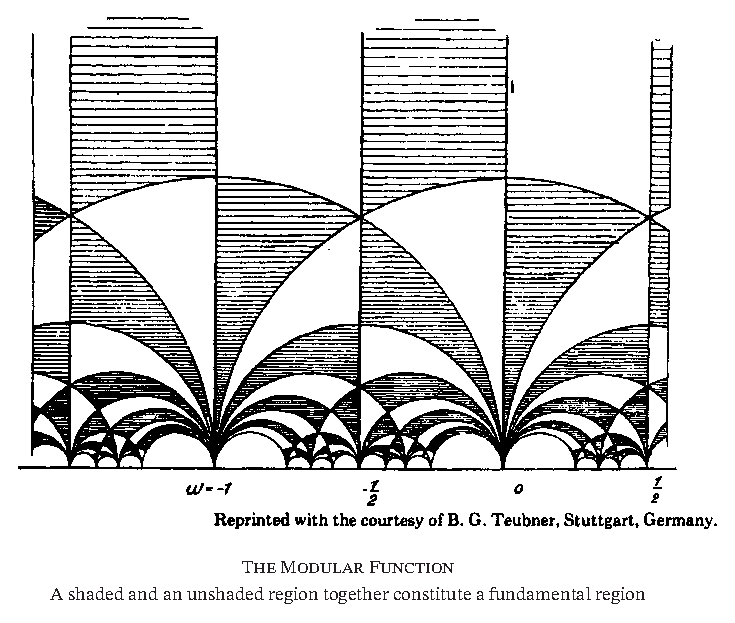
\includegraphics{chap01-vend-scan-01.eps}
\caption{}\index{notation}{$\Omega_{j}$}\index{notation}{$\Sigma_{j}$}
\label{fig1}
\end{figure}

\index{notation}{$d_{z}$}
\index{notation}{$\Lambda_{x},\ \Lambda(z)$}
\begin{align}\label{eq2.9}
\Lambda_{z}&=\left[\begin{array}{cccc}
1 & 1 & \cdots & 1\\
\alpha_{1}z & \alpha_{2}z & \cdots & \alpha_{n}z\\
(\alpha_{1}z)^{2} & (\alpha_{2}z)^{2} & \cdots & (\alpha_{n}z)^{2}\\
\cdots& & &\\
(\alpha_{1}z)^{n-1} & (\alpha_{2}z)^{n-1} & \cdots & (\alpha_{n}z)^{n-1 }
\end{array}\right]\\\nonumber
&=\left[\begin{array}{cccc}
1 & & & \\
& z & & \\
& & \ddots&\\
& & &z^{n-1}
\end{array}\right]\,\left[\begin{array}{cccc}
1 & 1 & \cdots & 1\\
\alpha_{1} & \alpha_{2} & \cdots & \alpha_{n}\\
\ldots& & &\\
\alpha_{1}^{n-1} & \alpha_{2}^{n-1} & \cdots & \alpha_{n}^{n-1}
\end{array}\right]\equiv d_{z}\Lambda(z).
\end{align}
Here $(\alpha_{1},\ldots, \alpha_{n})$ are the roots of unity in the ordering associated to $z$. When $z$ is understood we denote the diagonal matrix $J(z)$ and the Vandermonde matrix $\Lambda(z)$ by $J$ and $\Lambda$; they depend only on the sector $\Omega \subset \mathbf{C}\backslash \Sigma$.

\emph{Note that} $\Lambda_{z}$ \emph{diagonalizes} $J_{2}$:

\begin{equation}\label{eq2.10}
\Lambda_{z}^{-1}J_{z}\Lambda_{z}=zJ.
\end{equation}
In fact (\ref{eq2.10}) is clearly equivalent to
\begin{equation}\label{eq2.11}
J_{z}\Lambda_{z}=z\Lambda_{z}J,
\end{equation}
which can be established either by direct computation or by differentiating (\ref{eq2.8}) with respect to $x$ at $x=0$ and using the fact that $\varphi$ solves (\ref{eq2.1}) with $q=0$.



The problem (\ref{eq1.2}), (\ref{eq1.5}), (\ref{eq1.6}) becomes, for our system: given $z\in \mathbf{C}\backslash \Sigma$, determine (if possible) a matrix solution $\psi(\cdot, z)$ of (\ref{eq2.1}) with asymptotic properties\index{subject}{matrix solution, $\psi$, \S2}
\begin{equation*}\label{eq2.12-}
\tag*{$(2.12)_{-}$}\lim_{x\rightarrow-\infty} \psi(x, z)e^{-ixzJ}=\Lambda_{z},\index{notation}{$\psi$}
\end{equation*}
\begin{equation*}\label{eq2.12+}
\tag*{$(2.12)_{+}$}\mathop{\lim\sup}_{x\rightarrow+\infty}\Vert\psi(x,z)e^{-ixzJ}\Vert<\infty.
\end{equation*}
It is convenient to rewrite this problem by expressing $\psi$ in the form\index{subject}{fundamental matrix m, (2.13)}\index{notation}{$m$}
\setcounter{equation}{12}
\begin{equation}\label{eq2.13}
\psi(x, z)\ =m(x, z)e^{ixzJ}.
\end{equation}
Then our problem becomes\index{subject}{fundamental matrix m, (2.14)}\index{notation}{$m$}
\begin{align*}\label{eq2.14-}
\tag*{$(2.14)_{-}$}
\left\{\begin{array}{lll}D_{x}m=J_{z}m-zmJ+qm,&\\
\mathrm{lim}_{x\longrightarrow-\infty}\ m(x,z)=\Lambda_{z},&\\
m(\cdot,z)\text{ is bounded}.\end{array}\right.
\end{align*}\index{notation}{$\overset{\sim}{m}$}
Note the corresponding problem normalized at $+\infty$:
\begin{align*}\label{eq2.14+}
\tag*{$(2.14)_{+}$}\left\{\begin{array}{lll}D_{x}\tilde{m}=J_{z}\tilde{m}-z\tilde{m}J+q\tilde{m},&\\
\mathrm{lim}_{x\longrightarrow+\infty}\ \tilde{m}(x,z)=\Lambda_{z},&\\
\tilde{m}(\cdot,z) \text{ is bounded}.\end{array}\right.
\end{align*}
\begin{defi}
A \emph{fundamental matrix} for the operator $L$ and the point $ z\in \mathbf{C}\backslash \Sigma$ is a solution $m(\cdot,z)$ of (2.14)$_{-}$ or $(2.14)_{+}$.

Note that \emph{the determinant of a fundamental matrix is independent of} $x$, since
\begin{equation*}
D_{x}(\det m)=D_{x}(\det\psi)= \mathrm{tr} (J_{z}+q)\cdot \det\psi=0
\end{equation*}
    and so $\det m(\cdot, z)\equiv\det\Lambda_{z}$.
\end{defi}
\setcounter{theorem}{14}
\begin{prop}\label{prop2.15}
For $z\in \mathbf{C}\backslash \Sigma$,  each of the problems $(2.14)_{-}$ and $(2.14)_{+}$
has at most one solution.
\end{prop}

\begin{proof}
 Suppose that $m(\cdot, z)$ and $m'(\cdot,z)$ are solutions of $(2.14)_{-}$. Since $\det m(\cdot, z)$ is constant, $m^{-1}$ is bounded with respect to $x$. Therefore $m^{-1}m'$ is bounded. A simple computation shows that
\begin{equation*}
D_{x}(m^{-1}m')=[zJ, m^{-1}m']
\end{equation*}
where [$A$, $B$] denotes the commutator $AB-BA$. Therefore there is a constant matrix $A$ such that
\setcounter{equation}{15}
\begin{equation}\label{eq2.16}
m(x, z)^{-1}m'(x,z)=e^{ixzJ}Ae^{-ixzJ}.
\end{equation}
The $(j, k)$ entry of the matrix on the right in (\ref{eq2.16}) is
\begin{equation}\label{eq2.17}
e^{ixz(\alpha_{j}-\alpha_{k})}A_{j k}.
\end{equation}
When $j\neq k$, (\ref{eq2.17}) cannot be a bounded function of $x$ unless $A_{j k}=0$. Thus $A$ is a diagonal matrix. The asymptotic condition at $-\infty$ implies $A=I$ and $m\equiv m'$. The proof of uniqueness in $(2.14)_{+}$ is the same.
\end{proof}
\setcounter{theorem}{17}
\begin{remark}\label{eq2.18}
If $z\in\Sigma\backslash 0$, the preceding argument breaks down at precisely one point: one can have $A_{j k}\neq 0$ for those $(j,\ k)$ with $\mathrm{Re}(iz\alpha_{j})=\mathrm{Re}(iz\alpha_{k})$.
\end{remark}
Let $e_{1}, e_{2}, \ldots , e_{n}$ denote the standard basis vectors for $\mathbf{C}^{n}$ considered as a space of column vectors:\index{notation}{$e_{j}$}
\setcounter{equation}{18}
\begin{equation}\label{eq2.19}
e_{1}=(1,0,\ldots,0)^{t},\ e_{2}=(0,1,0,\ldots, 0)^{t}, \ldots.
\end{equation}
Then $m_{k}=me_{k}$ and $\tilde{m}_{k}=\tilde{m}e_{k}$ are the $k$th columns of the matrices $m,\ \tilde{m}$. They satisfy the differential equation
\begin{equation}\label{eq2.20}
D_{x}m_{k}=(J_{z}-\alpha_{k}zI+q)m_{k}
\end{equation}
with boundary conditions\label{eq2.21-}
\begin{align*}\tag*{$(2.21)_{-}$}
& \mathop\mathrm{lim}_{x\rightarrow-\infty} m_{k}(x,z)=\Lambda_{z}e_{k},\quad m_{k}(\cdot,z)\ \text{is bounded}; \\
\label{eq2.21+}\tag*{$(2.21)_{+}$}&  \mathop\mathrm{lim}_{x\rightarrow+\infty}\tilde{m}_{k}(x,z)=\Lambda_{z}e_{k},\quad\tilde{m}_{k}(\cdot,z)\ \text{is bounded}.
\end{align*}

By (\ref{eq2.10}), $i(J_{z}-\alpha_{k}zI)$ is similar to a normal operator with spectrum
\begin{equation*}
i(\alpha_{1}-\alpha_{k})z,\quad i(\alpha_{2}-\alpha_{k})z, \ldots,\quad i(\alpha_{n}-\alpha_{k})z.
\end{equation*}
The ordering (\ref{eq2.7}) implies that this operator has nonpositive real part when $k=1$ and nonnegative real part when $k=n$. Therefore the columns $m_{1}$ and $\tilde{m}_{n}$ can be obtained as solutions of Volterra equations
\begin{align*}\label{eq2.22-}
\tag*{$(2.22)_{-}$} m_{1}(x,z)&=\Lambda_{z}e_{1}+i\int_{-\infty}^{x} e^{i(x-y)(J_{z}-\alpha_{1}zI)}[q(y)m_{1}(y,z)]dy;\\
\tag*{$(2.22)_{+}$} \tilde{m}_{n}(x,z)&=\Lambda_{z}e_{n}-i\int_{x}^{\infty} e^{i(x-y)(J_{z}-\alpha_{n}zI)}[q(y)\tilde{m}_{n}(y,z)]dy.
\end{align*}

We shall discuss these equations more fully in \S3. For motivation and orientation we specialize in the next subsection to the \emph{second order case}. We also indicate the connections to other treatments of this case.

\setcounter{section}{1}
\section{bis. The Second Order Case}
When $n=2,$ the set $\Sigma$ is $\mathbf{R}$. The equations (2.22) give us two solutions for $z\notin \mathbf{R}$: \index{notation}{$u_{1}, \overset{\sim}{{u}_{2}}$}
\setcounter{equation}{22}
\begin{align}\label{eq2.23}
\left\{\begin{array}{ll}u_{1}(x,z)=m_{11}(x,z)\mathrm{exp}(\mp ixz),&\\
\tilde{u}_{2}(x,z)=\tilde{m}_{12}(x,z)\mathrm{exp}(\mp ixz),\quad \pm\ \mathrm{Im}\,z> 0.
\end{array}\right.
\end{align}
These are solutions of
\begin{equation}\label{eq2.24}
D^{2}u=z^{2}u+q_{1}u\equiv z^{2}u-pu.
\end{equation}
For more details about the various assertions which follow, see \cite{DT, Fa1} and the following sections.

The equations (2.22) make sense for $z\in \mathbf{R}$ and give boundary values\index{notation}{$u_{1}^{\pm},\ u_{2}^{\pm}$}
\begin{align}\label{eq2.25}
\left\{\begin{array}{ll}
u_{1}^{\pm}(x,s)={{\mathrm{lim}}\atop{\varepsilon\searrow 0}}\ u_{1}(x,s\pm i\varepsilon),&\\ \\
\tilde{u}_{2}^{\pm}(x,s)={{\mathrm{lim}}\atop{\varepsilon\searrow 0}}\ \tilde{u}_{2}(x,s\pm i\varepsilon),& \qquad s\ \in\ \mathbf{R}.\end{array}\right.
\end{align}
These solutions, for given $z$, are dependent if and only if the Wronskian $W(z)$ vanishes, where\index{notation}{$W(z)$}
\begin{equation}\label{eq2.26}
W(z)\equiv i\left|
             \begin{array}{cc}
               u_{1}(\cdot, z)& \tilde{u}_{2}(\cdot, z) \\
               Du_{1}(\cdot, z) & D\tilde{u}_{2}(\cdot, z) \\
             \end{array}
             \right|=i\left|
                        \begin{array}{cc}
                          m_{11} & \tilde{m}_{12} \\
                          m_{21} & \tilde{m}_{22} \\
                        \end{array}
                      \right|.
    \end{equation}
It will be useful to think of the Wronskian in connection with exterior algebra. The \emph{wedge product} $m_{1}\wedge\tilde{m}_{2}$ takes values in the exterior power $\Lambda^{2}(\mathbf{C}^{2})$ which has basis vector $e_{1}\wedge e_{2}$, and
\begin{equation*}
m_{1}\wedge\tilde{m}_{2}=\left|
                            \begin{array}{cc}
                              m_{11} & \tilde{m}_{12} \\
                               m_{21} & \tilde{m}_{22} \\
                            \end{array}
                          \right|\ e_{1} \wedge e_{2}.
\end{equation*}
The differential equations (\ref{eq2.20}) imply
\begin{align}\label{eq2.27}
D(m_{1}\wedge\tilde{m}_{2})&=(Dm_{1})\wedge\tilde{m}_{2}+m_{1}\wedge D\tilde{m}_{2}\\ \notag
&=\cdots= [\mathrm{tr}\ J_{z}-\alpha_{1}z-\alpha_{2}z+ \mathrm{tr}\ q]m_{1}\wedge\tilde{m}_{2}=0,
\end{align}
confirming that $W$ depends only on $z$.

Let us examine the asymptotics of the solutions $u_{1},\ \tilde{u}_{2}$. Clearly
\begin{align*}\label{eq2.28-}
\tag*{$(2.28)_{-}$} \qquad \quad &u_{1}(x,z)\sim\exp(\mp ixz)&\mathrm{as}\ x\rightarrow-\infty,
&\quad\pm\mathrm{Im}\ z>0;\\\label{eq2.28+}
\tag*{$(2.28)_{+}$}  \qquad \quad &\tilde{u}_{2}(x,z)\sim\exp(\pm ixz)&\mathrm{as}\ x\rightarrow+\infty,&\quad\pm\mathrm{ Im}\ z>0.
\end{align*}
Moreover, these asymptotics are also valid for the limits on $\mathbf{R}$. On the other hand, the operator $\exp(ix[J_{z}-\alpha_{1}zI])$ converges as $ x\rightarrow+\infty$ to the projection onto its null space, which is spanned by $\Lambda_{z}e_{1}$. Thus there is a scalar $\Delta$ such that
\begin{equation*}\label{eq2.29-}
\tag*{$(2.29)_{-}$}  m_{1}(x,z)\rightarrow\Delta(z)\Lambda_{z}e_{1}\ \mathrm{as}\  x\rightarrow+\infty,\quad \ z\not\in \mathbf{R}.
\end{equation*}
Similarly,\index{notation}{$\Delta,\ \overset{\sim}{\Delta}$}
\begin{equation*}\label{eq2.29+}
\tag*{$(2.29)_{+}$}  \tilde{m}_{2}(x, z)\rightarrow\tilde{\Delta}(z)\Lambda_{z}e_{2}\quad  \mathrm{as}\  x\rightarrow-\infty,\quad z\not\in \mathbf{R}.
\end{equation*}
Taking limits in (\ref{eq2.26}) we obtain
\setcounter{equation}{29}
\begin{equation}\label{eq2.30}
 W(z)=i\Delta(z)\det\ \Lambda_{z}=i\tilde{\Delta}(z)\det\Lambda_{z}.
\end{equation}
Thus $\Delta=\tilde{\Delta}$ and
\begin{align}\label{eq2.31}
&u_{1}(x,z)\sim\Delta(z)\exp(\mp ixz)\quad\mathrm{as}\ x\rightarrow+\infty,\\ \notag
&\tilde{u}_{2}(x,z)\sim\Delta(z)\exp(\pm ixz)\quad\mathrm{as}\ x\rightarrow-\infty, \quad\pm\mathrm{Im}\ z>0.
\end{align}
It follows from this that the full matrix $m(\cdot, z)$ exists when $\Delta(z)\neq 0$, and
\begin{equation}\label{eq2.32}
m_{2}(x, z)=\Delta(z)^{-1}\tilde{m}_{2}(x, z).
\end{equation}
The renormalized second solution is
\begin{equation}\label{eq2.33}
u_{2}(x, z)=\Delta(z)^{-1}\ \tilde{u}_{2}(x,z).
\end{equation}
Set\index{notation}{$\Delta^{\pm}(s)$}
\begin{equation}\label{eq2.34}
\Delta^{\pm}(s)=\mathop\mathrm{lim}_{\varepsilon\searrow 0}\Delta(s\pm i\varepsilon),\qquad s\in \mathbf{R}.
\end{equation}
The argument giving (\ref{eq2.31}) breaks down with $z\in \mathbf{R}$; one can obtain instead
\begin{align*}\label{eq2.35-}
\tag*{$(2.35)_{-}$} \qquad  &u_{1}^{\pm}(x,s)\sim\Delta^{\pm}(s)\exp(\mp ixs)+a^{\pm}(s)\exp(\pm ixs) &\mathrm{as}\ x\rightarrow+\infty, \\\label{eq2.35+}
\tag*{$(2.35)_{+}$} \qquad  &\tilde{u}_{1}^{\pm}(x,s)\sim\Delta^{\pm}(s)\exp(\pm ixs)+b^{\pm}(s)\exp(\mp ixs) &\mathrm{as}\ x\rightarrow-\infty.
\end{align*}

We are now in a position to give a tentative description of \emph{scattering data} for the second order operator $L=D^{2}+p$ and to relate our version to previous treatments of the second order case.
\setcounter{theorem}{35}
\begin{prop}\label{chap01:prop2.36}For $z_{0}\not\in \mathbf{R},\ D^{2}+p$  has an $L^{2}$-eigenfunction with
eigenvalue $z_{0}^{2}$ if and only if $\Delta(z_{0})=0$. If so, there is a constant $d(z_{0})$ such that $\tilde{u}_{2}(x, z_{0})\equiv d(z_{0})u_{1}(x, z_{0})$.
\end{prop}

\begin{proof}
 If $\Delta (z_{0})=0$, then the Wronskian vanishes and $\tilde{u}_{2}$ is a multiple of $u_{1}$. Since $u_{1}$ (resp. $\tilde{u}_{2}$) vanishes exponentially as $x\rightarrow-\infty ($resp. $x\rightarrow+\infty)$, there is an $L^{2}$ eigenfunction. If $\Delta(z_{0})\neq 0$, then any eigenfunction is a nontrivial linear combination of $u_{1}$ and $\tilde{u}_{2}$, and the asymptotics (2.28), (\ref{eq2.31}) exclude $L^{2}$.
 \end{proof}

For the rest of this section we \emph{assume} that $\triangle^{\pm}$ is nowhere zero on $\mathbf{R}\backslash 0$. Then for each $s\in \mathbf{R}\backslash 0,\ (u_{1}^{-}, u_{2}^{-})$ is a basis of solutions for $D^{2}+p-s^{2}$ and there is a unique $2\times 2$ matrix $V(s)$ such that
\setcounter{equation}{36}
\begin{equation}\label{eq2.37}
(u_{2}^{+}(x, s), u_{1}^{+}(x, s))\equiv(u_{1}^{-}(x, s), u_{2}^{-}(x,\ s))V(s).
\end{equation}
Later, we shall take the matrix function $V$, together with a slightly renormalized version of the set of constants $\{d(z_{0})\}$ of Proposition $2.36$, as the \index{subject}{scattering data, second order, (2.36) (2.37)}\emph{scattering data} for $D^{2}+p$.
\setcounter{theorem}{37}
\begin{prop}\label{chap01:prop2.38}
The matrix $V$  has the form
\setcounter{equation}{38}
\begin{equation}\label{eq2.39}
V(s)=\left(
  \begin{array}{cc}
    1+a(s)b(s) & a(s) \\
    b(s) & 1 \\
  \end{array}
\right).
\end{equation}
Moreover,
\begin{align}\label{eq2.40}
1+a(s)&b(s)=[\Delta_{+}(s)\Delta_{-}(s)]^{-1},\\
&b(s)=-a(-s).\label{eq2.41}
\end{align}
If $p$ is real, so $D^{2}+p$ is selfadjoint, then
\begin{equation}\label{eq2.42}
b(s)=-\overline{a(s)}.
\end{equation}
\end{prop}

\begin{proof}
The definitions, together with the asymptotics (2.28), (2.35), give
\begin{align*}
(e^{ixs}, e^{-ixs}) \left(\begin{array}{cc}
1 & 0\\
b^{+}/\Delta^{+} & 1
\end{array}\right)\sim(e^{ixs}, e^{-ixs}) \left(\begin{array}{cc}
1 & b^{-}/\Delta^{-}\\
0 & 1
\end{array}\right) V(s)
\end{align*}
as $ x\rightarrow-\infty$, which gives (\ref{eq2.39}) with $b=b^{+}/\Delta^{+}$ and $a=-b^{-}/\Delta^{-}$. Similarly, the asymptotics as $ x\rightarrow+\infty$ give (\ref{eq2.40}). The symmetry (\ref{eq2.41}) comes from the symmetry
\begin{equation*}
J_{-z}=J_{z},\qquad -z\alpha_{j}(-z)=z\alpha_{j}(z),
\end{equation*}
so that $m(x, -z)=m(x, z)$. Therefore
\begin{equation*}
u_{j}^{+}(s)=u_{j}^{-}(-s),\qquad s\in \mathbf{R},
\end{equation*}
which implies (\ref{eq2.41}). Finally, if $p$ is real then it is easy to check that $m(x, \overline{z})= \overline{m(x,z)}$ so
\begin{equation}\label{eq2.43}
u_{j}^{+}(s)=\overline{u_{j}^{-}(s)},
\end{equation}
which implies (\ref{eq2.42}). Note that (\ref{eq2.43}) and (2.35) imply
\begin{equation}\label{eq2.44}
\Delta^{+}=\overline{{\Delta^{-}}}\quad\text{if }p\text{ is  real}.
\end{equation}
\end{proof}
For the convenience of the reader, we make the connection here with treatments of the second order selfadjoint problem as in Faddeev \cite{Fa1} or Deift and Trubowitz \cite{DT}. (The notation in this part should be erased from memory upon passing to \S 3 and beyond!)

We follow Deift and Trubowitz and denote by $f_{j}(x,z)$ the Jost solutions (eigenfunctions) which are characterized for $z\in \mathbf{R}\backslash 0$ by the asymptotics
\begin{align*}
&f_{1}(x, z)\sim e^{ixz}\ \mathrm{as}\  x\rightarrow+\infty,\\
&f_{2}(x, z) \sim e^{-ixz}\ \mathrm{as}\  x\rightarrow-\infty.
\end{align*}
These solutions have holomorphic extensions to $\mathbf{C}_{+} = \{\mathrm{Im}\, z>0\}$, \, with $f_{1}(x, z) \exp(-ixz)$ and $f_{2}(x, z) \exp(ixz)$ bounded with respect to $x$. Thus in our notation
\begin{equation*}
f_{2}=u_{1}^{+},\quad f_{1}=\tilde{u}_{2}^{+}=\Delta^{+}u_{2}^{+}\qquad \mathrm{on}\,\ \mathbf{R}\backslash 0.
\end{equation*}
The \index{subject}{reflection coefficient, \S2-bis}\emph{reflection coefficients $R_{j}$ \emph{and} transmission coefficients}\index{subject}{transmission coefficient, \S2-bis} $T_{j}$ are uniquely determined by
\begin{align*}
&T_{1}(s)f_{2}(\cdot, s)=R_{1}(s)f_{1}(\cdot, s)+f_{1}(\cdot, -s),\\
&T_{2}(s)f_{1}(\cdot, s)\ =R_{2}(s)f_{2}(\cdot, s)+f_{2}(\cdot, -s),\qquad s\in \mathbf{R}\backslash 0.
\end{align*}
The asymptotics imply $f_{1}(\cdot, -s)=\tilde{u}_{2}^{-}(\cdot, s),\ f_{2}(\cdot, -s)=u_{1}^{-}(\cdot, s)$. Therefore the relationships can be written
\begin{equation*}
T_{1}u_{1}^{+}=R_{1}\Delta^{+}u_{2}^{+}+\Delta^{-}u_{2}^{-},\qquad T_{2}\Delta^{+}u_{2}^{+}=R_{2}u_{1}^{+}+u_{1}^{-},
\end{equation*}
or
\begin{equation*}
(u_{2}^{+}, u_{1}^{+}) \left(\begin{array}{@{}cc@{}}
-R_{1}\Delta^{+} & T_{2}\Delta^{+}\\
T_{1} & -R_{2}
\end{array}\right)=(u_{1}^{-},u_{2}^{-}) \left(\begin{array}{@{}cc@{}}
0 & 1\\
\Delta^{-} & 0
\end{array}\right).
\end{equation*}
But (\ref{eq2.37}), (\ref{eq2.39}), (\ref{eq2.40}) give
 \begin{equation*}
(u_{2}^{+}, u_{1}^{+}) \left(\begin{array}{@{}cc@{}}
1 & -a\\
-b & (\Delta^{-}\Delta^{+})^{-1}
\end{array}\right)=(u_{1}^{-},u_{2}^{-})
\end{equation*}
and so
\begin{equation*}
T_{1}=T_{2}=(\Delta^{+})^{-1},\qquad R_{2}=b,\qquad R_{1}=a\Delta^{-}(\Delta^{+})^{-1}.
\end{equation*}

Faddeev \cite{Fa1} introduces a matrix $S=(s_{ij})$ associated with normalized eigenfunctions $\psi_{j}(\cdot, k),\ k\in \mathbf{R}$:
\begin{align*}
&\psi_{1}(x,k)\sim\left\{\begin{array}{ll}
e^{ikx}+s_{12}(k)e^{-ikx}, & x\rightarrow-\infty,\\
s_{11}(k)e^{ikx}, & x\rightarrow+\infty;
\end{array}\right.\\
&\psi_{2}(x, k)\sim\left\{\begin{array}{ll}
e^{-ikx}+s_{21}(k)e^{ikx}, & x\rightarrow+\infty,\\
s_{22}(k)e^{-ikx}, & x\rightarrow-\infty.
\end{array}\right.
\end{align*}
Thus
\begin{align*}
&\psi_{1}=s_{11}\tilde{u}_{2}^{+}=u_{1}^{-}+s_{12}u_{1}^{+},\\
&\psi_{2}=s_{22}u_{1}^{+}=\tilde{u}_{2}^{-}+s_{21}\tilde{u}_{2}^{+},
\end{align*}
and so
\begin{equation*}
(u_{2}^{+}, u_{1}^{+}) \left(\begin{array}{@{}cc@{}}
s_{11}\Delta^{+} & -s_{21}\Delta^{+}\\
-s_{12} & -s_{22}
\end{array}\right)=(u_{1}^{-}, u_{2}^{-}) \left(\begin{array}{@{}cc@{}}
1 & 0\\
0 & \Delta^{-}
\end{array}\right).
\end{equation*}
Therefore the $S$-matrix is\index{subject}{\emph{S}-matrix, \S2-bis}
\begin{equation*}
(s_{jk})=\left(\begin{array}{@{}cc@{}}
1/\Delta^{+} & b\\
\Delta^{-}a/\Delta^{+} & 1/\Delta^{+}
\end{array}\right).
\end{equation*}
When $p$ is real we know that $\Delta^{+}=\overline{\Delta^{-}}$, and it follows from Proposition 2.38 that $S$ is \emph{unitary}.

\emph{Notational aside}. With $n=2$ and $\Sigma=\mathbf{R}$, it is natural to take the ``plus'' and ``minus'' sides of $\Sigma$ to correspond to $\mathbf{C}_{+}$ and $\mathbf{C}_{-}$ as in (\ref{eq2.25}) above. With $n >2$ and $\Sigma$ a union of rays from the origin it will be convenient to consider that one passes from the ``minus'' to the ``plus'' side of a given ray by crossing $\Sigma$ in the positive (counterclockwise) direction; see \S 11. Thus for $n=2$ the two notions coincide on $\mathbf{R}_{+}$ and are at odds on $\mathbf{R}_{-}$. From now until we return specifically to the second order case in \S 20 we shall use the convention corresponding to $n>2$. Thus the results as stated will be valid also for $n=2$, but with the $n >2$ convention; the reader is invited to convert various results to the natural convention for $n=2$.

\section{Fundamental tensors}\label{sec3}
As in \S 2 we let $e_{1},\ldots,e_{n}$ be the standard column basis vectors for $\mathbf{C}^{n}$ so that $m_{k}=me_{k}$ and $\tilde{m}_{k}=\tilde{m}e_{k}$ are the $k$th columns of $m$ and $\tilde{m}.$ Consider the wedge products with values in the exterior algebra \index{subject}{fundamental tensors, (3.1)}\index{subject}{tensors, fundamental, (3.1)} $\Lambda(\mathbf{C}^{n})=\bigoplus\Lambda^{k}(\mathbf{C}^{n})$:\index{notation}{$f_{k}$}\index{notation}{$g_{k}$}
\setcounter{equation}{0}
\begin{align}\label{eq3.1}
&f_{k}(\cdot, z)=m_{1}(\cdot,z)\wedge m_{2}(\cdot, z)\wedge\cdots \wedge m_{k}(\cdot,z),\\ \notag
&g_{k}(\cdot,z)=\tilde{m}_{k}(\cdot, z)\wedge\tilde{m}_{k+1}(\cdot,z)\wedge\cdots \wedge\tilde{m}_{n}(\cdot,z).
\end{align}\index{notation}{$m_{k}=me_{k}$}
The following elementary algebraic fact will allow us to interpret the differential equations arising from (\ref{eq2.20}) as equations for $\Lambda(\mathbf{C}^{n})$-valued functions.

So interpreted, these equations tell us how certain subspaces of solutions of the original equation vary with $x$.
\setcounter{theorem}{1}
\begin{prop}\label{chap01:prop3.2} Associated to a linear transformation $A$ : $ \mathbf{C}^{n}\rightarrow\ \mathbf{C}^{n}$ there is a unique linear map $A^{(k)}$ : $\Lambda^{k}(\mathbf{C}^{n})\rightarrow\Lambda^{k}(\mathbf{C}^{n})$ such that for all $ u_{1},\ldots, u_{k} \in \mathbf{C}^{n}$,\index{notation}{$A^{(k)}$}
\setcounter{equation}{2}
\begin{equation}\label{eq3.3}
A^{(k)}(u_{1}\wedge\cdots \wedge u_{k})=\sum_{j=1}^{k}u_{1}\wedge\cdots \wedge u_{j-1}\wedge Au_{j}\wedge u_{j+1}\wedge\cdots \wedge u_{k}.
\end{equation}
\end{prop}

\begin{pf} The right side of (\ref{eq3.3}) defines an alternating $k$-linear map from $\mathbf{C}^{n}$ to $\Lambda^{k}(\mathbf{C}^{n})$. By the universal property of the exterior product, this map extends uniquely to $\Lambda^{k}(\mathbf{C}^{n})$.
\end{pf}

In the notation of Proposition ~\ref{chap01:prop3.2}, the equations for $m_{j}$ and $\tilde{m}_{j}$ imply

\begin{align*}
&\tag*{$(3.4)_{-}$}  Df_{k}=[J_{z}^{(k)}-(\alpha_{1}+\cdots +\alpha_{k})zI+q^{(k)}]f_{k},\\ \notag
&\tag*{$(3.4)_{+}$}  Dg_{k}=[J_{z}^{(n-k+1)}-(\alpha_{k}+\cdots +\alpha_{n})zI+q^{(n-k+1)}]g_{k}.
\end{align*}
The asymptotic conditions are
\begin{equation*}
\tag*{$(3.5)_{-}$} \displaystyle \lim_{x\rightarrow-\infty} f_{k}(x, z)=\Lambda_{z}e_{1}\wedge\cdots\wedge\Lambda_{z}e_{n},
\end{equation*}
\begin{equation*}\label{eq3.35+}
\tag*{$(3.5)_{+}$}\displaystyle \lim_{x\rightarrow+\infty}  g_{k}(x,z)=\Lambda_{z}e_{k}\wedge \cdots\wedge\Lambda_{z}e_{n}.
\end{equation*}
\setcounter{theorem}{5}
\setcounter{equation}{7}
\begin{definition}\label{chap01:defi3.6}\index{subject}{fundamental tensor families, (3.6)}\index{subject}{tensor families, fundamental, (3.6)}
\emph{A fundamental tensor family} for the operator $L$ and for $
z\in \mathbf{C}\backslash \Sigma$ is a set of solutions $\{f_{k},
g_{k}\}$ to the problem (3.4)--(3.5), $1\leq k\leq n$.
\end{definition}

\begin{theorem}\label{chap01:thm3.7}
For each $ z\in \mathbf{C}\backslash \Sigma$ there is a unique fundamental tensor family for $L$ and $z$. On each component $\Omega$ of $ \mathbf{C}\backslash \Sigma$ these families are holomorphic with respect to $z;$ they extend to $\overline{\Omega}\backslash 0$ so as to be in $C^{\infty}(\mathbf{R}\times(\overline{\Omega}\backslash 0))$ and these extensions satisfy \emph{(3.5)}.
\end{theorem}

The proof of Theorem ~\ref{chap01:thm3.7} occupies the rest of this section. The idea is simply that, like $f_{1}=m_{1}$ and $g_{n}=\tilde{m}_{n}$, all the $f_{k}$ and $g_{k}$ are solutions of Volterra equations.

Consider the operators occurring in (3.4):\index{notation}{$A_{z,k}$}\index{notation}{$B_{z,k}$}
\begin{align}\label{eq3.8}
&A_{z,k}\equiv J_{z}^{(k)}-\ (\alpha_{1}+\cdots +\alpha_{k})zI,\\ \notag
&B_{z,k}\equiv J_{z}^{(n-k+1)}-\ (\alpha_{k}+\cdots +\alpha_{n})zI.
\end{align}
The standard basis $e_{1},\ldots,e_{n}$ gives rise to the standard basis for $\Lambda^{k}(\mathbf{C}^{n})$:
\begin{equation}\label{eq3.9}
\{e_{j_{1}}\wedge\cdots\wedge e_{jk}:1\leq j_{1}< j_{2}<\cdots <j_{k}\leq n\}.
\end{equation}
We equip $\Lambda^{k}(\mathbf{C}^{n})$ with the inner product for which this basis is orthonormal.
\setcounter{theorem}{9}
\begin{prop}\label{chap01:prop3.10}
A linear transformation A in $\mathbf{C}^{n}$ has a unique extension to a linear map of $\Lambda(\mathbf{C}^{n})$ to itself such that for all $ u_{1},\ldots, u_{k}\in \mathbf{C}^{n}$
\setcounter{equation}{10}
\begin{equation}\label{eq3.11}
A(u_{1}\wedge\cdots\wedge u_{k})=Au_{1}\wedge\cdots\wedge Au_{k}.
\end{equation}
This extension preserves products and adjoints.
\end{prop}

\begin{pf}
As in the proof of Proposition ~\ref{chap01:prop3.2}, the right side of (\ref{eq3.11}) defines an alternating $k$-linear map. The extension obviously preserves products and is easily verified to preserve adjoints.
\end{pf}
\setcounter{theorem}{11}
\begin{lemma}\label{chap01:lem3.12}
The operators $A_{z,k}$ and $B_{z,k}$ of \emph{(3.8)} satisfy
\setcounter{equation}{12}
\begin{align}\label{eq3.13}
&A_{z,k}=\Lambda_{z}[zA_{k}]\Lambda_{z}^{-1},\\ \notag
&B_{z,k}=\Lambda_{z}[zB_{k}]\Lambda_{z}^{-1},
\end{align}
where $A_{k}$ and $B_{k}$ are the normal operators
\index{notation}{$A_{k}$}\index{notation}{$B_{k}$}
\begin{align}\label{eq3.14}
&A_{k}=J^{(k)}-\ (\alpha_{1}+\cdots +\alpha_{k})I, \\ \notag
&B_{k}=J^{(n-k+1)}-(\alpha_{k}+\cdots +\alpha_{n})I.
\end{align}
The spectrum of $izA_{k}$ $($resp. $izB_{k})$ lies in the left $($resp. right$)$ half plane of $\mathbf{C}$\emph{:}
\end{lemma}
\begin{align}\label{eq3.15}
&\mathrm{spec}(izA_{k})=\{iz(\alpha_{j_{1}}+\cdots +\alpha_{j_{k}}-\alpha_{1}-\cdots -\alpha_{k}):j_{1}<j_{2}<\cdots <j_{k}\}; \\ \notag
&\mathrm{spec}(izB_{k})=\{iz(\alpha_{j_{k}}+\cdots+\alpha_{j_{n}}-\alpha_{k}-\cdots-\alpha_{n}):j_{k}<j_{k+1}<\cdots<j_{n}\}.
\end{align}

\begin{pf}
The identities (\ref{eq3.13}) follow from (\ref{eq2.10}) and Proposition 3.10. The remaining statements are immediate, since the standard basis vectors (\ref{eq3.9}) are eigenvectors of the $A_{k}$ and $B_{k}$ with eigenvalues (\ref{eq3.15}).
\end{pf}
It will be convenient to transform our fundamental tensor families to take advantage of the diagonalization (\ref{eq3.13}). Set\index{subject}{tensor families, transformed, (3.16)}\index{notation}{$f_{k}^{\#}$}
\begin{equation}\label{eq3.16}
f_{k}^{\#}=\Lambda_{z}^{-1}f_{k},\qquad g_{k}^{\#}=\Lambda_{z}^{-1}g_{k}.
\end{equation}\index{notation}{$g_{k}^{\#}$}
These are to be solutions of
\begin{align*}\label{eq3.17-}
&\tag*{$(3.17)_{-}$} \left\{\begin{array}{ll}
\frac{d}{dx}f_{k}^{\#}=izA_{k}f_{k}^{\#}+iq_{k}^{\#}f_{k}^{\#},\\\notag
\lim_{x\rightarrow-\infty}f_{k}^{\#}(x, z)=e_{1}\wedge e_{2}\wedge\cdots \wedge e_{k};
\end{array}\right.\\ \notag
&\tag*{$(3.17)_{+}$}  \quad \left\{\begin{array}{ll}
\frac{d}{dx}g_{k}^{\#}=izB_{k}g_{k}^{\#}+iq_{n-k+1}^{\#}g_{k}^{\#},\\ \notag
\lim_{x\rightarrow+\infty}g_{k}^{\#} (x, z)=e_{k}\wedge e_{k+1}\wedge\cdots\wedge e_{n}.
\end{array}\right.\\
\end{align*}
Here\index{notation}{$q_{k}^{\#}$}
\setcounter{equation}{17}
\begin{equation}\label{eq3.18}
q_{k}^{\#}(x, z)=\Lambda_{z}^{-1}q^{(k)}(x)\Lambda_{z}=\sum_{j^{=1}}^{m(k)}z^{-j}q_{kj}(x).
\end{equation}
Note that only negative powers occur in (\ref{eq3.18}), because of the form of the matrix $q$.

The $2n$ problems (3.17) can be discussed by considering a single\index{subject}{abstract (Volterra) model, (3.21)} \emph{abstract model}. Let $V$ be a finite-dimensional hermitian vector space with norm $\Vert\,\Vert$ and let $A\in \mathscr{L}(V)$ be a normal operator. Let\index{notation}{$\Omega_{A}$}
\begin{equation}\label{eq3.19}
\Omega_{A}=\{z\in \mathbf{C}:zA+\overline{z}A^{*}\leq 0\}.
\end{equation}
We assume that $\Omega_{A}$ has nonempty interior; thus $\Omega_{A}$ is a proper closed sector in $\mathbf{C}$. Suppose
\begin{equation}\label{eq3.20}
q(x, z)=\sum_{j=1}^{m}z^{-j}q_{j}(x), \qquad q_{j}\in \mathscr{S}(\mathbf{R};\mathscr{L}(V)).
\end{equation}
For $z\in\Omega_{A}\backslash 0$ and a fixed $u_{0}\in \mathrm{ker}\,A$ we consider the problem
\begin{equation}\label{eq3.21}
\left\{\begin{array}{l}
\frac{d}{dx}u=zAu+q(\cdot, z)u,\\
\lim_{x\rightarrow-\infty}u(x)=u_{0}.
\end{array}\right.
\end{equation}
(The problem $(3.17)_{-}$ has exactly this form; changing $x$ to $-x$ brings $(3.17)_{+}$ to this form.)

\begin{pothm}\label{pot3.7}
We need only consider the more general abstract model (\ref{eq3.21}). If $u$ satisfies (\ref{eq3.21}), then for any real $s$ and $x$ it satisfies the integral equation
\begin{equation}\label{eq3.22}
u(x)=e^{(x-s)zA}u(s)+\int_{s}^{x}e^{(x-y)zA}q(y, z)u(y)\ dy.
\end{equation}
Now $zA$ is normal with nonpositive real part, so $\exp(tzA)$ has norm $\leq 1$ for $t\geq 0$. Therefore we may take the limit as $ s\rightarrow-\infty$ in (\ref{eq3.22}) to obtain
\begin{equation}\label{eq3.23}
u(x)=u_{0}+\int_{-\infty}^{x}e^{(x-y)zA}q(y, z)u(y)\ dy.
\end{equation}
Conversely, any solution of the Volterra integral equation (\ref{eq3.23}) which is bounded as $ x\rightarrow-\infty$ solves (\ref{eq3.21}). The usual procedure gives the unique solution of (\ref{eq3.23}) as the limit of the Picard iterates
\begin{equation}\label{3.24}
\left\{\begin{array}{l}
u_{0}(x)\equiv u_{0},\\
u_{\nu+1}(x)=u_{0}+\int_{-\infty}^{x}e^{(x-y)zA}q(y,z)u_{\nu}(y) dy.
\end{array}\right.
\end{equation}
One obtains inductively the estimates
\begin{align}\label{eq3.25}
&\Vert u_{\nu}(x)-u_{\nu-1}(x)\Vert\leq\frac{1}{\nu!}Q(x, z)^{\nu}\Vert u_{0}\Vert,\\ \notag
&\qquad Q(x, z)=\int_{-\infty}^{x}\Vert q(y, z)\Vert dy.
\end{align}
Thus the solution $u$ is a bounded function of $x$:
\begin{equation}\label{eq3.26}
\Vert u(x)\Vert\leq\Vert u_{0}\Vert e^{Q(x,z)}.
\end{equation}

To complete the proof we nerd to consider the solution $u$ to (\ref{eq3.23}) as a function $u(\cdot, z)$ of $z,\ z\in\Omega_{A}\backslash 0$. The Picard iterates (3.24) are continuous on $\mathbf{R}\times(\Omega_{A}\backslash 0)$ and are holomorphic with respect to $z$ in the interior of $\Omega_{A}$. Convergence is locally uniform on $\mathbf{R} \times\ (\Omega_{A}\backslash 0)$, so $u$ is holomorphic in $z$ on the interior of $\Omega_{A}$ and continuous on $\mathbf{R}\ \times\ (\Omega_{A}\ \backslash 0)$. The differential equation implies that each $x$-derivative is continuous on $\mathbf{R}\times(\Omega_{A}\backslash 0)$.

To investigate smoothness with respect to $z$ we differentiate the Picard iterates to obtain
\begin{align}\label{eq3.27}
v_{\nu+1}(x, z)&\equiv\frac{\partial}{\partial z}u_{\nu+1}(x,z)-xAu_{\nu+1}(x,z)\\ \notag
&=f_{\nu}(x, z)+\int_{-\infty}^{x}e^{(x-y)zA}[qv_{\nu}]dy.
\end{align}
Here
\begin{equation}\label{eq3.28}
f_{\nu}(x, z)=\int_{-\infty}^{x}e^{(x-y)zA}\left\{[q,yA]u_{\nu}+\frac{\partial q}{\partial z}u_{\nu}\right\}dy.
\end{equation}
The estimates (\ref{eq3.25}) imply
\begin{align}\label{eq3.29}
\Vert f_{\nu}(x,z)-f_{\nu-1}(x,z)\displaystyle \Vert & \leq\frac{1}{v!}Q(x, z)^{\nu}\Vert u_{0}\Vert\int_{-\infty}^{x}\left\Vert[q, yA]+\frac{\partial q}{\partial z}\right\Vert dy\\ \notag
&\equiv\frac{1}{\nu!}Q(x, z)^{\nu}R(x, z)\Vert u_{0}\Vert\equiv\varepsilon_{\nu}(x, z).
\end{align}
Inductively, (\ref{eq3.27}) and (\ref{eq3.29}) give
\begin{equation}\label{3.30}
\Vert v_{\nu}-v_{\nu-1}\Vert\leq\sum_{j=0}^{\nu-1}\frac{1}{j!}\varepsilon_{\nu-j}Q^{j}.
\end{equation}
Therefore the $v_{\nu}$ converge to $\partial u/\partial z-zAu$ and we have the estimate
\begin{align}\label{eq3.31}
\left\Vert\frac{\partial}{\partial z}u(x,z)-xAu(x,z)\right\Vert &\leq e^{Q(x, z)}\sum_{\nu=1}^{\infty}\varepsilon_{n}(x,z)\\ \notag
&=e^{2Q(z,z)-1}R(x,z)\Vert u_{0}\Vert.
\end{align}
Further $z$-derivatives are handled in the same way.
\end{pothm}

\section{Behavior of fundamental tensors as $|x|\rightarrow\infty$; the functions $\Delta_{k}$}\label{sec4} In this section we obtain the general analogue of the asymptotic results (2.29) in the case $n=2$.
\setcounter{theorem}{0}
\begin{theorem}\label{thm4.1}
There are scalar functions $\Delta_{k}(z),\ 0\leq k\leq n$, holomorphic on $ \mathbf{C}\backslash \Sigma$, and having smooth extensions to $\overline{\Omega}\backslash 0$, such that on $ \mathbf{C}\backslash \Sigma$\index{notation}{$\Delta_{k}$}
\begin{equation*}
\tag*{$(4.2)_{-}$} \displaystyle \lim_{x\rightarrow+\infty}  f_{k}(x,z)=\Delta_{k}(z)\Lambda_{z}e_{1}\wedge\cdots \wedge\Lambda_{z}e_{k};
\end{equation*}
\begin{equation*}
\tag*{$(4.2)_{+}$} \displaystyle \lim_{x\rightarrow-\infty}  g_{k+1}(x, z)=\Delta_{k}(z)\Lambda_{z}e_{k+1}\wedge\cdots \wedge\Lambda_{z}e_{n}.
\end{equation*}
\renewcommand\theequation{\thesection.\arabic{equation}}
\setcounter{equation}{2}
\begin{equation}\label{eq4.3}
f_{k}(x,z)\wedge g_{k+1}(x,z)\equiv\Delta_{k}(z)\Lambda_{z}e_{1}\wedge\cdots \wedge\Lambda_{z}e_{n}.
\end{equation}
Moreover,
\begin{equation*}
\tag*{$(4.4)_{-}$} \Delta_{n}\equiv 1,\qquad  f_{n}(x, z)\equiv\Lambda_{z}e_{1}\wedge\cdots \wedge\Lambda_{z}e_{n};
\end{equation*}
\begin{equation*}
\tag*{$(4.4)_{+}$} \Delta_{0}\equiv 1,\qquad  g_{1}(x,z)\equiv\Lambda_{z}e_{1}\wedge\cdots \wedge\Lambda_{z}e_{n}.
\end{equation*}
The functions $\Delta_{k}$ are given by the integral formulas
\begin{equation*}
\tag*{$(4.5)_{-}$} \Delta_{k}(z) =1+\displaystyle \frac{i}{n}\int_{\mathbf{R}}(q^{(k)}(y)f_{k}(y, z), (\Lambda_{z}^{-1})^{*}(e_{1}\wedge\cdots \wedge e_{k})) dy,
\end{equation*}
\begin{equation*}
\tag*{$(4.5)_{+}$} \Delta_{k}(z)=1-\frac{i}{n}\int_{\mathbf{R}}(q^{(n-k)}(y)g_{k+1}(y, z), (\Lambda_{z}^{-1})^{*}(e_{k+1}\wedge\cdots \wedge e_{n}))\ dy,
\end{equation*}
where \emph{(\,,\,)} denotes the inner products in $\Lambda^{k}(\mathbf{C}^{n})$ and in $\Lambda^{n-k}(\mathbf{C}^{n})$.
\end{theorem}

\begin{pf}
The product $f_{k}\wedge g_{k+1}$ satisfies the differential equation
\begin{equation*}
\frac{d}{dx}h=i\ [J_{z}^{(n)}-z(\alpha_{1}+\cdots +\alpha_{n})+q^{(n)}]h=i[J_{z}^{(n)}-q^{(n)}]h.
\end{equation*}
Now, $A^{(n)}$ is the operation of multiplication by the trace of $A$, so $f_{k}\wedge g_{k+1}$ is constant with respect to $x$. Moreover, the matrix $\Lambda_{z}$ is invertible for $z\neq 0$, so $\Lambda_{z}(e_{1}\wedge\cdots \wedge e_{n})\neq 0$. Therefore (\ref{eq4.3}) defines functions $\Delta_{k}$. This argument also proves (4.4). Theorem ~\ref{chap01:thm3.7} implies that the $\Delta_{k}$ defined by (\ref{eq4.3}) are holomorphic and extend smoothly to $\overline{\Omega}\backslash 0$.

To establish (4.2) and (4.5) we return to the model problem (\ref{eq3.21}) of the last section. Suppose the nonzero eigenvalues of the normal operator $A$ have negative real part. Then $\exp(tA)$ converges $ t\rightarrow+\infty$ to the orthogonal projection onto the kernel of $A$, and the solution of $u$ of the integral equation (\ref{eq3.23}) is asymptotically
\begin{equation*}
u_{0}+\mathrm{Proj}_{\mathrm{ker}\,A}\left\{\int_{\mathbf{R}}q(y, z)u(y)dy\right\}.
\end{equation*}
In our case the operators $A_{k}$ and $B_{k+1}$ have one-dimensional kernels spanned by $\Lambda_{z}(e_{1}\wedge\cdots\wedge e_{k})$ and by $\Lambda_{z}(e_{k+1}\wedge\cdots\wedge e_{n})$; see Lemma ~\ref{chap01:lem3.12}. For $ z\in\Omega$ the nonzero eigenvalues have negative (resp. positive) real part. Therefore
\begin{equation*}
\tag*{$(4.6)_{-}$} \displaystyle \lim_{x\rightarrow+\infty}  f_{k}(x, z)=\Delta_{k}'(z)\Lambda_{z}e_{k}\wedge\cdots\wedge\Lambda_{k}e_{n},
\end{equation*}
\begin{equation*}
\tag*{$(4.6)_{+}$} \displaystyle \lim_{x\rightarrow-\infty} g_{k+1}(x, z)=\Delta_{k}''(z)\Lambda_{z}e_{k+1}\wedge\cdots\wedge\Lambda_{k}e_{n}.
\end{equation*}
It follows immediately from (4.6) and (\ref{eq4.3}) that $\Delta_{k}'=\Delta_{k}=\Delta_{k}''$.

Our argument gives the integral formulae
\begin{equation*}
\tag*{$(4.7)_{-}$}\qquad \qquad \quad \displaystyle \Delta_{k}=1+i\int_{\mathbf{R}}(q_{k}^{\#}f_{k}^{\#}, e_{1}\wedge\cdots\wedge e_{k}) dy,
\end{equation*}
\begin{equation*}
\tag*{$(4.7)_{+}$} \qquad \qquad \quad \displaystyle \Delta_{k}=1-i\int_{\mathbf{R}}(q_{n-k}^{\#}g_{k+1}^{\#},e_{k+1}\wedge\cdots\wedge e_{n}) dy.
\end{equation*}
Now $q_{k}^{\#}f_{k}^{\#}=\Lambda_{z}^{-1}(q^{(k)}f_{k})$ and $q_{n-k}^{\#}g_{k+1}^{\#}=\Lambda_{z}^{-1}[q^{(n-k)}g_{k+1}]$. Therefore (4.7) implies (4.5).
\end{pf}
\setcounter{theorem}{7}
\begin{remark}\label{chap01:thm4.8}
The asymptotics (4.2) are not generally true on $\Sigma$. However, if $z\in\Sigma\backslash 0$ is on the boundary of a sector with ordering $(\alpha_{1}, \ldots, \alpha_{n})$ and if
\setcounter{equation}{8}
\begin{equation}\label{eq4.9}
\mathrm{Re}(i\alpha_{k}z)\neq\mathrm{Re}(i\alpha_{k+1}z)
\end{equation}
then $(4.2)_{\pm}$ hold. The proof is the same as for $ z\not\in\Sigma$.
\end{remark}

\section{Behavior of fundamental tensors as $ z\rightarrow\infty$} The fundamental tensor families have full asymptotic expansions as $z \rightarrow\infty$ in a closed sector $\overline{\Omega}$.
\setcounter{theorem}{0}
\begin{theorem}\label{chap01:thm5.1}
There are unique bounded smooth functions
\begin{equation*}
f_{k\nu}^{\#}:\mathbf{R}\rightarrow\Lambda^{k}(\mathbf{C}^{n}),\qquad g_{k\nu}^{\#}:\mathbf{R}\rightarrow\Lambda^{n-k+1}(\mathbf{C}^{n}),
\end{equation*}
$\nu=0,1,2,\ldots,$ such that\index{notation}{$f_{k\nu}^{\#}$}\index{notation}{$g_{k\nu}^{\#}$}
\begin{equation*}
\tag*{$(5.2)_{-}$} \qquad \qquad \quad f_{k}(x, z)\displaystyle \sim\sum_{\nu=0}^{\infty}z^{-\nu}\Lambda_{z}f_{k\nu}^{\#}(x)\quad \mathrm{as}\ z\rightarrow\infty,
\end{equation*}
\begin{equation*}
\tag*{$(5.2)_{+}$} \qquad \qquad \quad g_{k}(x, z)\displaystyle \sim\sum_{\nu=0}^{\infty}z^{-\nu}\Lambda_{z}g_{k\nu}^{\#}(x)\quad \mathrm{as}\ z\rightarrow\infty.
\end{equation*}
Here $(5.2)_{-}$ means that for $N\in \mathbf{Z}_{+}$ there is a constant $C_{kN}$ such that
\renewcommand{\theequation}{\thesection.\arabic{equation}}
\setcounter{equation}{2}
\begin{equation}\label{eq5.3}
\left\Vert\Lambda_{z}^{-1}f_{k}(x,z)-\sum_{\nu\leq N}z^{-\nu}f_{k\nu}^{\#}(x)\right\Vert\leq C_{kN}|z|^{-N-1}
\end{equation}
for $x\in \mathbf{R}$ and $z\in\overline{\Omega},\ |z|\geq 1$. The meaning of $(5.2)_{+}$ is similar. Moreover,
\begin{equation}\label{eq5.4}
f_{k0}^{\#}\equiv e_{1}\wedge\cdots \wedge e_{k},\qquad  g_{k0}^{\#}\equiv e_{k}\wedge\cdots \wedge e_{n},
\end{equation}
\begin{align}\label{eq5.5}
&\lim_{x\rightarrow-\infty}\ f_{k\nu}^{\#}(x)=0,\qquad \nu >0,\\ \notag
&\lim_{x\rightarrow+\infty}\ g_{k\nu}^{\#}(x)=0,\qquad \nu >0.
\end{align}
\end{theorem}

\begin{pf}
It is enough to obtain the analogous result for the abstract model (\ref{eq3.19})--(3.21). We want to establish

\begin{equation}\label{eq5.6}
u(x,z)\sim\sum_{\nu=0}^{\infty}z^{-\nu}u_{\nu}(x)\ \mathrm{as}\  z\rightarrow\infty,\ z\in\Omega_{A}.
\end{equation}
For any $v\in V$ write
\begin{equation}\label{eq5.7}
v=v'+v'',\qquad v'\in \mathrm{ker}\,A,\ v''\perp \mathrm{ker}\,A.
\end{equation}
Since $A$ is normal, $\mathrm{ker}\,A= (\mathrm{ran}\,A)^{\perp}$ and $A$ has a unique partial inverse
\begin{equation*}
A^{-1} : \mathrm{ran}\, A\rightarrow(\mathrm{ker}A)^{\perp},\qquad A^{-1}=0\ \mathrm{on}\ \mathrm{ker}\,A.
\end{equation*}
The $u_{\nu}$ in (\ref{eq5.6}) are clearly unique. We determine candidates for these functions recursively by a formal differentiation of (\ref{eq5.6}). This differentiation leads to
\begin{equation}\label{eq5.8}
\frac{d}{dx}u_{\nu}=Au_{\nu+1}+\sum_{k=1}^{m}q_{k}u_{\nu-k},
\end{equation}
where $u_{\nu}\equiv 0$ for $\nu <0$. The decomposition (\ref{eq5.7}) converts (\ref{eq5.8}) to
\begin{equation}\label{eq5.9}
\left\{\begin{array}{l}
u_{\nu+1}''=A^{-1}\{\frac{d}{dx}u_{\nu}-\sum_{k=1}^{m}q_{k}u_{\nu-k}\}\\
\frac{d}{dx}u_{\nu}'=\sum_{k=1}^{m}(q_{k}u_{\nu-k})'.
\end{array}\right.
\end{equation}
If we impose the natural conditions

\begin{equation}\label{eq5.10}
\lim_{x\rightarrow-\infty} u_{0}(x)=u_{0},\qquad \lim_{x\rightarrow-\infty}\ u_{\nu}(x)=0,\qquad \nu >0,
\end{equation}
then (\ref{eq5.9}), (\ref{eq5.10}) is equivalent to
\begin{equation}\label{eq5.11}
\left\{\begin{array}{l}
u_{0}(x)\equiv u_{0},\\
u_{\nu+1}(x)=\int_{-\infty}^{x}\sum(q_{k}u_{\nu+1-k})'dy+A^{-1}\{\frac{d}{dx}u_{\nu}-\sum q_{k}u_{\nu-k}\}
\end{array}\right..
\end{equation}
Since the $q_{k}$ are assumed to be Schwartz functions, we obtain inductively

\begin{equation}\label{eq5.12}
\frac{d}{dx}u_{\nu}'\in \mathscr{S}(\mathbf{R};V),\qquad u_{\nu}''\in \mathscr{S}(\mathbf{R}; V).
\end{equation}

To complete the proof we must show that the $u_{\nu}$ defined by (\ref{eq5.11}) satisfy (\ref{eq5.6}) in the sense of (\ref{eq5.3}). Let
\begin{equation*}
v_{N}(x, z)=\sum_{j=0}^{N}z^{-j}u_{j}(x),\qquad z\in\Omega_{A}\backslash 0.
\end{equation*}
Then (\ref{eq5.8}) implies
\begin{equation*}
\frac{d}{dx}v_{N}=(zA+q)v_{N}+r_{N},
\end{equation*}
where $r_{N}$ is a polynomial in $z^{-1}$ with coefficients belonging to $\mathscr{S}(\mathbf{R};V)$. Moreover,

\begin{equation}\label{eq5.13}
\int_{\mathbf{R}}\Vert r_{N}(x,z)\Vert\, dx\leq C_{N}|z|^{-N},\qquad |z|\geq 1.
\end{equation}
Therefore $w_{N}=u-v_{N}$ satisfies
\begin{equation}\label{eq5.14}
\left\{\begin{array}{l}
\frac{d}{dx}w_{N}=(zA+q)w_{N}-r_{N},\\
\lim_{x\rightarrow-\infty}w_{N}(x, z)=0.
\end{array}\right.
\end{equation}
As in the proof of Theorem $3.7,(5.14)$ is equivalent to an integral equation
\begin{equation}\label{eq5.15}
w_{N}(x, z)=\int_{-\infty}^{x}e^{(x-y)zA}[qw_{N}-r_{N}]dy.
\end{equation}
The first Picard approximation to the solution of (\ref{eq5.15}) satisfies
\begin{equation*}
\Vert w_{N0}(x, z)\Vert\leq\int_{-\infty}^{x}\Vert r_{N}(y, z)\Vert dy\leq C_{N}|z|^{-N}
\end{equation*}
for $|z|\geq 1$. The remaining iterates then satisfy

\begin{align*}
&\Vert w_{N\nu}(x, z)-w_{N,\nu-1}(x, z)\Vert\leq\frac{\mathbf{1}}{\nu!}C_{N}|z|^{-N}Q(x)^{\nu},\\
&\qquad\quad Q(x)=\sup_{|z|\geq 1}\int_{-\infty}^{x}\Vert q(y, z)\Vert dy.
\end{align*}
Therefore for $z\in\Omega_{A}$ and $|z|\geq 1$ we have
\begin{equation*}
\tag*{$(5.16)_{N}$} \qquad \qquad \quad \Vert u(x,z)-v_{N}(x, z)\Vert\leq C_{N}|z|^{-N}e^{Q(x)}.
\end{equation*}
The sharper estimate with $|z|^{-N-1}$ on the right follows from $(5.16)_{N+1}$, since $v_{N+1}-v_{N}=O(|z|^{-N-1})$.
\end{pf}
\setcounter{theorem}{16}
\begin{remark}\label{chap01:rem5.17}
This result could also be proved by repeated integration by parts in the integral equation for $f_{k}$ or $g_{k}$.
\end{remark}

\begin{cor}\label{chap01:coro5.18}
The function $\Delta_{k}$ of Theorem \emph{4.1} have asymptotic expansions
\setcounter{equation}{18}
\begin{equation}\label{eq5.19}
\Delta_{k}(z)\sim 1+\sum_{\nu=1}^{\infty}d_{k\nu}z^{-\nu}
\end{equation}
as $z\rightarrow\infty$, uniformly in $\overline{\Omega}$.
\end{cor}

\section{Behavior of fundamental tensors as $z\rightarrow
0$}\label{sec6}There are two competing features of the problem
(3.4)--(3.5) to consider as $z\rightarrow 0$. First, the boundary data in (3.5) tends to $0$ as $z\rightarrow 0$, except for $f_{1}$ and $g_{n}$. Second, since the norm of $\Lambda_{z}^{-1}$ as a linear transformation on $\Lambda^{k}(\mathbf{C}^{n})$ blows up as $z\rightarrow 0$ and since $A_{z,k}$ becomes nilpotent, it is not obvious how to control the $x$-behavior of
\begin{equation*}
\exp(ixA_{z,k})\ =\Lambda_{z}\,\exp(ixzA_{k})\Lambda_{z}^{-1}
\end{equation*}
as $z\rightarrow 0$. We deal with the first problem by renormalizing the tensor families. The second problem can be overcome at the expense of introducing powers of $x$ into the estimates.

The datum $\Lambda_{z}e_{1}\wedge\cdots\wedge\Lambda_{z}e_{k}$ is a polynomial in $z$ whose first nonvanishing term is
\setcounter{equation}{0}
\begin{equation}\label{eq6.1}
V(\alpha_{1}, \alpha_{2},\ldots,\alpha_{k})z^{k(k-1)/2}e_{1}\wedge\cdots \wedge e_{k}
\end{equation}

where $V$ is the Vandermonde determinant\index{notation}{$V(\alpha_{1}, \ldots, \alpha_{k})$}
\begin{equation}\label{eq6.2}
\left\{\begin{array}{ll}
V(\alpha_{1})=1 & \\
V(\alpha_{1},\ldots,\alpha_{k})=\left|\begin{array}{cccc}
                                      1 & 1 & \cdots & 1 \\
                                      \alpha_{1} & \alpha_{2} & \cdots & \alpha_{k} \\
                                      \cdots &  &  &  \\
                                      {\alpha_{1}^{k-1}} & {\alpha_{2}^{k-1}} & \cdots & {\alpha_{k}^{k-1}}
                                    \end{array}\right|
=\prod_{1\leq i<j\leq k}(\alpha_{j}-\alpha_{i}),\quad k>1.
\end{array}\right.
\end{equation}
Therefore we shall consider the behavior as $z\rightarrow 0$ of
\begin{equation}\label{eq6.3}
z^{-k(k-1)/2}f_{k}(x, z),\qquad z^{-(n-k+1)(n-k)/2}g_{k}(x, z).
\end{equation}
\setcounter{theorem}{3}
\begin{lemma}\label{chap01:lem6.4}
For $x\geq 0$ and $z\in\overline{\Omega},\ |z|\leq 1$,
\end{lemma}
\setcounter{equation}{4}
\begin{equation}\label{eq6.5}
\Vert\exp(ixA_{z,k})\Vert\leq C_{nk}(1+x^{k(n-k)}).
\end{equation}
\begin{pf}
It follows easily from (\ref{eq2.9}) that on $\Lambda^{k}(\mathbf{C}^{n}),\, \Vert\Lambda_{z}\Vert\sim\Vert d(z)\Vert= O(|z|^{0+1+\cdots +(k-1)})$. Similarly, $\Lambda_{z}^{-1}$ has norm which is $O(|z|^{1-n+\cdots +(k-n)})$. Combining,
\begin{equation}\label{eq6.6}
\Vert\Lambda_{z}\Vert\,\Vert\Lambda_{z}^{-1}\Vert\leq C_{nk}'|z|^{-k(n-k)},\quad 0<|z|\leq 1.
\end{equation}
Let $p=k(n -k)$. Note that
\begin{equation*}
\left|e^{w}-\sum_{j=0}^{p-1}\frac{1}{j!}w^{j}\right|\leq C_{p}|w|^{p}\quad \text{if Re } w\leq 0.
\end{equation*}
Since $ixzA_{k}$ is a normal operator with nonpositive real part we deduce
\begin{align*}
\Bigg\Vert \exp &(ixA_{z,k})\left. -\sum_{j^{=0}}^{p-1}\frac{1}{j!}(ixzA_{k})^{j}\right\Vert\\
&\leq\Vert\Lambda_{z}\Vert\left\Vert\exp(ixzA_{k})-\sum_{j=0}^{p-1}\frac{1}{j!}(ixzA_{k})^{j}\right\Vert\Vert\Lambda_{z}^{-1}\Vert\\
&\leq C_{nk}'C_{p}\Vert xA_{k}\Vert^{p},
\end{align*}
as the factors $|z|^{-p},\ |z|^{p}$ cancel. But
\begin{equation*}
\left\Vert\sum_{j=0}^{p-1}\frac{1}{j!}(ixA_{z,k})^{j}\ \right\Vert\leq C_{p}'(1+\Vert xA_{z,k}\Vert^{p-1})
\end{equation*}
and we obtain (\ref{eq6.5}) for $z\neq 0$. Taking the limit gives the result at $z=0$.
\end{pf}
\setcounter{theorem}{6}
\begin{theorem}\label{chap01:thm6.7}
There are unique smooth functions
\setcounter{equation}{7}
\begin{equation}\label{eq6.8}
f_{k\nu}:\ \mathbf{R}\rightarrow\Lambda^{k}(\mathbf{C}^{n}),\qquad g_{k\nu}:\mathbf{R}\rightarrow\Lambda^{n-k+1}(\mathbf{C}^{n}),
\end{equation}
$\nu=0,1,2,\ldots$ such that as $z\rightarrow 0,\ z\in\overline{\Omega}\backslash 0$, \index{notation}{$f_{k\nu}$}
\begin{equation*}
\tag*{$(6.9)_{-}$}  z^{-k(k-1)/2}f_{k}(x, z)\displaystyle \sim\sum_{\nu=0}^{\infty}z^{\nu}f_{k\nu}(x),
\end{equation*}\index{notation}{$g_{k\nu}$}
\begin{equation*}
\tag*{$(6.9)_{+}$}  z^{-(n-k+1)(n-k)/2}g_{k}(x,z)\displaystyle \sim\sum_{\nu=0}^{\infty}z^{\nu}g_{k\nu}(x).
\end{equation*}
Here \emph{(6.9)}-means that for $N\in \mathbf{Z}_{+}$,
\setcounter{equation}{9}
\begin{equation}\label{eq6.10}
\left\Vert z^{-k(k-1)/2}f_{k}(x,z)-\sum_{\nu\leq N}z^{\nu}f_{k_{\nu}}(x)\right\Vert\leq
C_{Nk}(x_{1})|z|^{N+1},
\end{equation}
for $x\leq x_{1},\ z\in\overline{\Omega}\backslash 0$, and $|z|\leq 1$. The meaning of $(6.9)_{+}$ is similar\emph{:} with $x\geq x_{1}$. The leading terms $f_{k0}$ and $g_{k0}$ are the unique solutions of
\begin{align*}
\tag*{$(6.11)_{-}$}   \left\{\begin{array}{l}
\frac{d}{dx}f_{k0}=iJ_{0}^{(k)}f_{k0}+iq^{(k)}f_{k0},\\
\\
\lim_{x\rightarrow-\infty}f_{k0}= V(\alpha_{1},\ldots,\alpha_{k})e_{1}\wedge\cdots\wedge e_{k},
\end{array}\right.
\end{align*}
\begin{align*}
\tag*{$(6.11)_{+}$}   \left\{\begin{array}{l}
\frac{d}{dx}g_{k0}=iJ_{0}^{(n-k+1)}g_{k0}+iq_{k0}^{(n-k+1)}g_{k0},\\
\\
\lim_{x\rightarrow+\infty}g_{k0}= V(\alpha_{k},\ldots,\alpha_{n})e_{1}\wedge\cdots\wedge e_{n-k+1}.
       \end{array}\right.
\end{align*}
Thus $f_{10}$ and $g_{n0}$ are independent of the sector $\Omega$.

Note that the asymptotics \emph{(6.11)} are very different from the
asymptotics \emph{(3.5)}, $z\neq 0!$
\end{theorem}
\begin{proof}
As before, it is convenient to consider a more general abstract model. Let $V$ be a finite-dimensional Hermitian vector space with norm $\Vert\cdot\Vert$. Let $q$ belong to $\mathscr{S}(\mathbf{R}; \mathscr{L}(V))$. Consider polynomial functions in $z$:
\begin{equation*}
A_{z}=\sum z^{j}A_{j}\in \mathscr{L}(V),\qquad u^{0}(z)=\sum z^{j}u_{j}^{0}\in V,
\end{equation*}
with
\setcounter{equation}{11}
\begin{equation}\label{eq6.12}
A_{z}u_{0}(z)\equiv 0,
\end{equation}
\begin{equation}\label{eq6.13}
\Vert\exp(xA_{z})\Vert\leq C(1+x^{p}),\qquad x\geq 0,\ z\ \in\overline{\Omega}.
\end{equation}
Then, for each $z\in\overline{\Omega}$, there is a unique solution $u=u(\cdot, z)$ to
\begin{equation}\label{eq6.14}
\left\{\begin{array}{ll}
\frac{d}{dx}u=A_{z}u+qu,\\
\\
\lim_{x\rightarrow-\infty}u(x, z) =u^{0}(z).
\end{array}\right.
\end{equation}
Indeed, we can look for $u=u^{0}+v$ where
\begin{equation}\label{eq6.15}
\left\{\begin{array}{ll}
\frac{d}{dx}v =A_{z}v+qv +qu^{0},\\
\\
\lim\nolimits_{x\rightarrow-\infty}v(x, z)=0,
\end{array}\right.
\end{equation}
which is equivalent to
\begin{align}\label{eq6.16}
v(x, z)&=r(x, z)+\int_{-\infty}^{x}e^{(x-y)A_{z}}q(y)v(y, z)\ dy,\\\nonumber
r(x, z)&=\int_{-\infty}^{x}e^{(x-y)A_{z}}q(y)u^{0}(z)dy.
\end{align}
Now, $r$ is rapidly decreasing as $x \rightarrow-\infty$; in fact,
\begin{equation*}
\Vert r(x, z)\Vert\leq C\int_{-\infty}^{x}(1-y)^{p}\Vert q(y)u^{0}(z)\Vert dy=Q(x)
\end{equation*}
for $x\leq 0$. The Picard argument then shows that (\ref{eq6.16}) has a unique solution $v$, with
\begin{equation}\label{eq6.17}
\Vert v(x,z)\ \Vert\leq Q(x)e^{Q(x)},\quad x\leq 0.
\end{equation}

We want to establish an asymptotic expansion as $z\rightarrow 0,\ z\in\overline{\Omega}$:
\begin{equation}\label{eq6.18}
v(x, z)\sim\sum_{\nu=0}^{\infty}z^{\nu}v_{\nu}(x).
\end{equation}
Formally, (\ref{eq6.15}) gives the sequence of problems

\begin{equation}\label{eq6.19}
\displaystyle \frac{d}{dx}v_{\nu}=\sum A_{j}v_{\nu-j}+qv_{\nu} +qu_{\nu}^{0}=(A_{0}+q)v_{\nu}+\left(\sum_{j>0}A_{j}v_{\nu-j}+qu_{\nu}^{0}\right),
\end{equation}
where $u_{\nu}^{0}=0$ for large $\nu$. The solution for $\nu=0$ is
$v_{0}(x)\equiv v(x, 0)$, and one can solve recursively for the
remaining $v_{\nu}$. Indeed, each of these problems has the same
structure as $($\ref{eq6.16}$)$. We set $\nu^{N}$ $=\sum_{\nu\leq N}z^{\nu}v_{\nu}$ and observe that $w_{N}=v-v^{N}$ satisfies
\begin{equation*}
\frac{d}{dx}w_{N}=A_{z}w_{N}+qw_{N}+z^{N+1}r_{N}(x,z)
\end{equation*}
when $N\geq\deg u^{0}$, where $r_{N}$ is a polynomial in $z$ whose coefficients vanish rapidly as $ x\rightarrow-\infty$. Moreover, $w_{N}\rightarrow 0$ as $ x\rightarrow-\infty$. The analogue of (\ref{eq6.17}) gives
\begin{equation}\label{eq6.20}
\Vert w_{N}(x,z)\Vert\leq C_{N}|z|^{N+1}S_{N}(x),
\end{equation}
where $S_{N}$ is rapidly decreasing as $ x\rightarrow-\infty$.

The zero-order term in the expansion of $u$ in (\ref{eq6.14}) is $u_{0}^{0}+v_{0}$, which satisfies
\begin{equation*}
\left\{\begin{array}{l}
\frac{d}{dx}(u_{0}^{0}+v_{0})=(A_{0}+q)(u^{0}+v_{0}),\\
\lim_{x\rightarrow-\infty}(u_{0}^{0}+v_{0})=u_{0}^{0}.
\end{array}\right.
\end{equation*}
This completes the proof of Theorem ~\ref{chap01:thm6.7}.
\end{proof}
\setcounter{theorem}{20}
\begin{cor}\label{chap01:coro6.21}
The functions $\Delta_{k}$ of Theorem \emph{\ref{thm4.1}} have asymptotic expansions as $z\rightarrow 0$ in $\overline{\Omega}$\emph{:}\index{notation}{$\Delta_{k\nu}$}
\setcounter{equation}{21}
\begin{equation}\label{eq6.22}
\Delta_{k}(z)\sim z^{k(k-n)}\sum_{\nu=0}^{\infty}\Delta_{k\nu}z^{\nu},
\end{equation}
where
\begin{equation}\label{eq6.23}
n\Delta_{k\nu}e_{1}\wedge\cdots\wedge e_{n}=\pm\sum_{j=0}^{\nu}f_{kj}\wedge g_{k+1,\nu-j},
\end{equation}
where the sign depends on $\Omega$.
\end{cor}
\begin{proof}
Note that
\begin{equation*}
\Lambda_{z}(e_{1}\wedge\cdots\wedge e_{n})=(\det\Lambda_{z})e_{1}\wedge\cdots\wedge e_{n}=\pm nz^{n(n-1)/2}e_{1}\wedge\cdots\wedge e_{n},
\end{equation*}
where the sign depends on $\Omega$, and
\begin{equation*}
k(n-k)=\tfrac{1}{2}n(n-1)-\tfrac{1}{2}k(k-1)-\tfrac{1}{2}(n-k)(n-k-1).
\end{equation*}
Therefore, using (\ref{eq4.3}),
\begin{align*}
\pm\, n&z^{k(n-k)}\Delta_{k}(z)e_{1}\wedge\cdots\wedge e_{n}\\
&=z^{-k(k-1)/2}z^{-(n-k)(n-k-1)/2}\Delta_{k}(z)\Lambda_{z}(e_{1}\wedge\cdots \wedge e_{n})\\
&\equiv(z^{-k(k-1)/2}f_{k})\wedge(z^{-(n-k)(n-k-1)/2}g_{k+1})\\
&\sim\left(\sum_{\nu=0}^{\infty}z^{\nu}f_{k\nu}\right)\wedge\left(\sum_{\nu=0}^{\infty}z^{\nu}g_{k+1,\nu}\right).
\end{align*}
\end{proof}

We shall be particularly interested in the leading terms of the expansions (\ref{eq6.22}).
\setcounter{theorem}{23}
\begin{cor}\label{chap01:coro6.24}
The function $\Delta_{k}$ of Theorem $\ref{thm4.1}$ satisfy
\setcounter{equation}{24}
\begin{equation}\label{eq6.25}
\Delta_{k}(z)=z^{k(k-n)}\Delta_{k0}+O(z^{k(k-n)+1}),
\end{equation}
as $z\rightarrow 0$ in $\overline{\Omega}$, where
\begin{align}\label{eq6.26}
\triangle_{k0}&=\pm\frac{i}{n}\int_{\mathbf{R}}(q^{(k)}(y)f_{k0}(y), e_{1}\wedge\cdots\wedge e_{k})dy\\
&=\mp\frac{i}{n}\int_{\mathbf{R}}(q^{(n-k)}(y)g_{k+1,0}(y), e_{1}\wedge\cdots\wedge e_{n-k})dy.\notag
\end{align}
\end{cor}
\begin{proof}
Since (\ref{eq6.25}) is contained in (\ref{eq6.22}), we need only show that (\ref{eq6.26}) follows from (\ref{eq6.23}) and the integral equations for $f_{k0},\ g_{k+1,0}$. Note that
\begin{equation*}
e^{tJ_{0}}\ (e_{1}\wedge e_{2}\wedge\cdots\wedge e_{p})=e_{1}\wedge e_{2}\wedge\cdots\wedge e_{p}.
\end{equation*}
Therefore
\begin{align*}
n\triangle_{k0}e_{1}\wedge\cdots\wedge e_{n}&\equiv f_{k0}\wedge g_{k+1,0}\\
&=\lim_{x\rightarrow\infty}f_{k0}(x)\wedge e_{1}\wedge\cdots\wedge e_{n-k}\\
&=\lim_{x\rightarrow\infty}i\int_{-\infty}^{x}[e^{i(x-y)J_{0}}q^{(k)}(y)f_{k0}(y)]\wedge e_{1}\wedge\cdots\wedge e_{n-k}\,dx\\
&=i\int_{\mathbf{R}}[q^{(k)}(y)f_{k0}(y)]\wedge e_{1}\wedge\cdots\wedge e_{n-k}\,dy.
\end{align*}
This last expression gives the first identity in (\ref{eq6.26}). The second identity is obtained by looking at the limit $ x\rightarrow-\infty$.
\end{proof}
\section{Construction of fundamental matrices}\label{sec7}
Starting from the fundamental tensor families $\{f_{k}, g_{k}\}$ for $L$ on a sector $\overline{\Omega}\backslash 0$, we want to construct the columns of the matrices $m$ and $\tilde{m}$, i.e., the solutions to (\ref{eq2.20})--(2.21). The first step is to show that the fundamental \index{subject}{decomposable tensors, (7.1)}\index{subject}{tensors, decomposable, (7.1)}tensors are \emph{decomposable}, i.e.,
\begin{equation*}
 f_{k}=v_{1}\wedge\cdots\wedge v_{k},\qquad  g_{k}=w_{k}\wedge\cdots\wedge w_{n},
\end{equation*}
for some vector-valued functions $v_{j},\ w_{j}$.

\begin{lemma}\label{chap01:lem7.1}
Suppose $u_{1}, u_{2},\ldots,u_{k}$ are vectors in $\mathbf{C}^{n}$ with $ u_{1}\wedge u_{2}\wedge\cdots\wedge u_{k}\neq$ $0$. Given $g\in\Lambda^{k+1}(\mathbf{C}^{n})$, the equation
\begin{equation*}
u_{1}\wedge u_{2}\wedge\cdots\wedge u_{k}\wedge v=g
\end{equation*}
has a solution of $v$ if and only if $u_{j}\wedge g=0,\, 1\leq j\leq k$.
\end{lemma}
\begin{proof}
Necessity of $u_{j}\wedge g=0$ is obvious. Extend $\{u_{j}\}$ to a basis and expand $g$ as a combination of the corresponding basis vectors
\begin{equation*}
u_{j_{\,1}}\wedge u_{j_{\,2}}\wedge\cdots\wedge u_{j_{k+1}},\qquad 1\leq j_{1}< j_{2}<\cdots<j_{k+1}\leq n.
\end{equation*}
Then $u_{j}\wedge g=0$ for $j\leq k$ implies that each nonzero term in this expansion of $g$ is a multiple of $ u_{1}\wedge\cdots\wedge u_{k}$.
\end{proof}
\begin{lemma}\label{chap01:lem7.2}
For each $z\in\overline{\Omega}\backslash 0$, there are unique smooth functions $v_{j}(\cdot, z) : \mathbf{R}\rightarrow \mathbf{C}^{n}$ and $w_{j}(\cdot,z) : \mathbf{R}\rightarrow \mathbf{C}^{n}$ such that
\setcounter{equation}{2}
\begin{equation}\label{eq7.3}
v_{1}\wedge\cdots\wedge v_{k}\equiv f_{k},\qquad  w_{k}\wedge\cdots\wedge w_{n}\equiv g_{k},
\end{equation}
\begin{equation}\label{eq7.4}
\left\{\begin{array}{ll}
v_{1},\ldots, v_{k} & \text{are orthogonal},\\
w_{k},\ldots, w_{n} & \text{are orthogonal}.
\end{array}\right.
\end{equation}
These functions satisfy
\begin{equation}\label{eq7.5}
v_{j}\wedge f_{l}\equiv 0,\ g_{j}\wedge w_{l}\equiv 0\qquad \text{if } j\leq l;
\end{equation}
\begin{equation*}
\tag*{$(7.6)_{-}$}   f_{k-1}\wedge(D-J_{z}-q+\alpha_{k}z)v_{k}\equiv 0,\qquad k>1;
\end{equation*}
\begin{equation*}
\tag*{$(7.6)_{+}$} [(D-J_{z}-q+\alpha_{k}z)w_{k}]\wedge g_{k+1}\equiv 0,\quad k<n.
\end{equation*}
\end{lemma}
\begin{proof}
We consider only the $v_{k}$. Necessarily $v_{1}=f_{1}$. Now, $v_{1}\wedge f_{k}$ is the solution of a first order homogeneous differential equation with zero initial condition:
\setcounter{equation}{6}
\begin{equation}\label{eq7.7}
\left\{\begin{array}{l}
[D-J_{z}^{(k+1)}+\alpha_{1}+ (\alpha_{1}+\cdots+\alpha_{k})z-q^{(k+1)}](v_{1}\wedge f_{k})\\
\qquad\,=[(D-J_{z}+\alpha_{1}z-q)v_{1}]\wedge f_{k}\\
\qquad\qquad\quad+v_{1}\wedge (D-J_{z}^{(k)}+ (\alpha_{1}+\cdots+\alpha_{k})z-q^{(k)})f_{k}\\
\qquad\,\equiv 0;
\end{array}\right.
\end{equation}
\begin{equation}\label{eq7.8}
\lim_{x\rightarrow-\infty}\  v_{1}(x, z)\wedge f_{k}(x, z)=\Lambda_{z}e_{1}\wedge\Lambda_{z}e_{1}\wedge\cdots =0.
\end{equation}
As in the proof of Theorem ~\ref{chap01:thm3.7}, the problem (\ref{eq7.7}), (\ref{eq7.8}) has the unique solution $v_{1}\wedge f_{k}\equiv 0$.

Suppose that $ v_{1},\ldots,v_{k-1}$ have been determined so as to satisfy (\ref{eq7.3}), (\ref{eq7.4}), (\ref{eq7.5}), $(7.6)_{-}$. Note that $ v_{1}\wedge\cdots\wedge v_{k-1}=f_{k-1}$ is everywhere nonzero, since it solves a first-order homogeneous differential equation with nonzero limit. By Lemma ~\ref{chap01:lem7.1}, the equation $f_{k-1}\wedge v=f_{k}$ will have a solution $v$ provided $v_{j}\wedge f_{k} \equiv 0$ for $j<k$. This is part of our induction assumption, so there is a solution $v_{k}$; the requirement that $v_{k}$ be orthogonal to $ v_{1},\ldots$, $v_{k-1}$ makes it unique. It is easily seen that $v_{k}$ is smooth with respect to $x$. To check $(7.6)_{-}$ we observe that
\begin{align*}
f_{k-1}&\wedge(D-J_{z}+\alpha_{k}z-q)v_{k}\\
&=(D-J_{z}^{(k)}+ (\alpha_{1}+\cdots+\alpha_{k})z-q^{(k)})f_{k}\\
&-[(D-J_{z}^{(k-1)}+ (\alpha_{1}+\cdots+\alpha_{k-1})z-q^{(k-1)})f_{k-1}]\wedge v_{k}\\
&=0.
\end{align*}
Therefore for each $x$,
\begin{equation}\label{eq7.9}
(D-J_{z}+\alpha_{k}z-q)v_{k}(x, z)\in \mathrm{span}\{v_{1}(x, z),\ldots,v_{k-1}(x, z)\}.
\end{equation}
Finally, if $l\geq k$ then we have
\begin{align}\label{eq7.10}
[D-J_{z}^{(l+1)}+(\alpha_{k}+\alpha_{1}+\cdots+\alpha_{l})&z-q^{(l+1)}](v_{k}\wedge f_{l})\\
&=[(D-J_{z}+\alpha_{k}z-q)v_{k}]\wedge f_{l}+0.\notag
\end{align}
The right-hand side of (\ref{eq7.10}) vanishes, by (\ref{eq7.9}) and the induction assumption. Moreover,
\begin{align*}
\displaystyle \lim_{x\rightarrow-\infty} v_{k}(x, z)\wedge f_{l}(x, z)&= \displaystyle \lim_{x\rightarrow-\infty}  v_{k}(x,z)\wedge\Lambda_{z}e_{1}\wedge\cdots\wedge\Lambda_{z}e_{l}\\
&=\ \lim_{x\rightarrow-\infty}\  v_{k}\wedge v_{1}\wedge\cdots\wedge v_{k}\wedge\Lambda_{z}e_{k+1}\wedge\cdots\wedge\Lambda_{z}e_{l}\\
&=0.
\end{align*}
Therefore $v_{k}\wedge f_{l}=0$ for $l\geq k$ and the induction step is verified.
\end{proof}

The next lemma is the key step in passing from the $v_{k}$ to the $m_{k}$.
\setcounter{theorem}{10}
\begin{lemma}\label{chap01:lem7.11}
Suppose $f_{k-1} \in\Lambda^{k-1}(\mathbf{C}^{n})$, $f_{k} \in\Lambda^{k}(\mathbf{C}^{n})$,\quad and\quad $g_{k} \in$ $\Lambda^{n-k+1}(\mathbf{C}^{n})$ are decomposable elements with
\setcounter{equation}{11}
\begin{equation}\label{eq7.12}
f_{k}=f_{k-1}\wedge v_{k},\qquad f_{k-1}\wedge g_{k}\neq 0.
\end{equation}
Then there is a unique $m_{k}\in \mathbf{C}^{n}$ such that
\begin{equation}\label{eq7.13}
f_{k-1}\wedge m_{k}=f_{k},\qquad m_{k}\wedge g_{k}=0.
\end{equation}
Moreover, the entries of $m_{k}$ can be expressed locally as rational functions of the coefficients of $f_{k-1},\ f_{k}$, and $g_{k}$ with respect to the standard bases.
\end{lemma}
\begin{proof}
Let $f_{k-1}$ and $g_{k}$ have the decompositions
\begin{equation*}
 f_{k-1}=u_{1}\wedge\cdots\wedge u_{k-1},\qquad  g_{k}=u_{k}\wedge\cdots\wedge u_{n}.
\end{equation*}
Then $\{u_{j}\}$ is a basis. Expressing $v_{k}$ as $\sum c_{j}u_{j}$, we see that the unique solution of (\ref{eq7.13}) is
\begin{equation*}
m_{k}=\displaystyle\sum_{j\geq k}c_{j}u_{j}.
\end{equation*}
To prove the statement about the coefficients with respect to the standard basis in $\Lambda(\mathbf{C}^{n})$, we use the standard inner product in $\Lambda(\mathbf{C}^{n})$ and express (\ref{eq7.13}) as
\begin{align}\label{eq7.14}
(f_{k-1}\wedge\, &m_{k}, e_{i_{1}}\wedge\cdots\wedge e_{i_{k}})=(f_{k}, e_{i_{1}}\wedge\cdots\wedge e_{i_{k}}),\\
&(m_{k}\wedge g_{k}, e_{i_{1}}\wedge\cdots\wedge e_{i_{n-k+2}})=0.\notag
\end{align}
This amounts to an overdetermined linear system for the coefficients of $m_{k}$. Since it has a unique solution, some subset of $n$ equations has nonzero determinant. Solving this subsystem gives the coefficients of $m_{k}$ (locally) as rational functions of those of $f_{k-1}, f_{k}, g_{k}$.
\end{proof}
\setcounter{theorem}{14}
\begin{theorem}\label{chap01:thm7.15}
Suppose $z\in\overline{\Omega}\backslash 0$ and $\triangle_{k-1}(z)\neq 0$. Then there is a unique bounded function $m_{k}(\cdot, z):\mathbf{R}\rightarrow \mathbf{C}^{n}$ with the properties
\setcounter{equation}{15}
\begin{equation}\label{eq7.16}
[D-J_{z}+\alpha_{k}z-q]m_{k}=0,
\end{equation}
\begin{equation*}
\tag*{$(7.17)_{-}$}\displaystyle \lim_{x\rightarrow-\infty} \Lambda_{z}e_{1}\wedge\cdots\wedge\Lambda_{z}e_{k-1}\wedge m_{k}=\Lambda_{z}e_{1}\wedge\cdots\wedge\Lambda_{z}e_{k},
\end{equation*}
\begin{equation*}
\tag*{$(7.18)_{-}$}\displaystyle \lim_{x\rightarrow+\infty}  m_{k}\wedge\Lambda_{z}e_{k+1}\wedge\cdots\wedge\Lambda_{z}e_{n}=\Delta_{k-1}(z)^{-1}\Delta_{k}(z)\Lambda_{z}e_{k}\wedge\cdots\wedge\Lambda_{z}e_{n}.
\end{equation*}
If $ z\in\Omega$ or $k=1$, or, more generally, if $\mathrm{Re}(i\alpha_{k-1}z)\neq\mathrm{Re}(i\alpha_{k}z)$, then \emph{(7.17)}$_{-}$ may be replaced by the stronger assertion
\begin{equation*}
\tag*{$(7.19)_{-}$} \displaystyle \lim_{x\rightarrow-\infty} m_{k}(x, z)=\Lambda_{z}e_{k}.
\end{equation*}
If $ z\in\Omega$ or $k=n$, or, more generally, if $\mathrm{Re}(i\alpha_{k}z)$ $\neq\mathrm{Re}(i\alpha_{k+1}z)$, then $(7.18)_{+}$ may be replaced by the stronger assertion
\begin{equation*}
\tag*{$(7.20)_{-}$} \displaystyle \lim_{x\rightarrow+\infty} m_{k}(x, z)=\Delta_{k-1}(z)^{-1}\Delta_{k}(z)\Lambda_{z}e_{k}.
\end{equation*}
\end{theorem}
\begin{proof}
By (\ref{eq4.3}), our assumption implies $f_{k-1}(x, z)\wedge g_{k}(x, z)\neq 0$, for all $x$. Lemma ~\ref{chap01:lem7.11} tells us there is a unique $m_{k}(x, z)$ with
\setcounter{equation}{20}
\begin{equation}
f_{k-1}\wedge m_{k}\equiv f_{k},\qquad m_{k}\wedge g_{k}\equiv 0.
\end{equation}
Since $m_{k}$ depends smoothly on $f_{k-1}$ and $g_{k}$, it is a smooth bounded function of $x$. Together with (3.4), the equations (7.21) imply
\begin{equation*}
f_{k-1}\wedge[D-J_{z}+\alpha_{k}z-q]m_{k}=0,
\end{equation*}
\begin{equation*}
[D-J_{z}+\alpha_{k}z-q]m_{k}\wedge g_{k}=0.
\end{equation*}
But $f_{k-1}\wedge g_{k}\neq 0$, so these equations imply (\ref{eq7.16}). The expression on the left in $(7.17)_{-}$ is the same as the limit of $f_{k-1}\wedge m_{k}=f_{k}$, which gives the right side of $(7.17)_{-}$. The second equation in (7.21) implies that $m_{k}\wedge g_{k+1}=c(x)g_{k}$. Then
\begin{equation*}
c\,(x)f_{k-1}\wedge g_{k}=f_{k-1}\wedge m_{k}\wedge g_{k+1}=f_{k}\wedge g_{k+1},
\end{equation*}
and (\ref{eq4.3}) implies $c(x)\equiv\Delta_{k-1}^{-1}\Delta_{k}$. Thus
\begin{equation}\label{eq7.22}
m_{k}\wedge g_{k+1}\equiv\Delta_{k-1}^{-1}\Delta_{k}g_{k},
\end{equation}
which implies $(7.18)_{-}$.

Suppose now that $\mathrm{Re}(i\alpha_{k-1}z)\neq\mathrm{Re}(i\alpha_{k}z)$. Theorem ~\ref{thm4.1} and Remark 4.8 entail
\begin{equation*}
\lim_{x\rightarrow-\infty}\  g_{k}(x, z)=\Delta_{k-1}(z)\Lambda_{z}e_{k}\wedge\cdots\wedge\Lambda_{z}e_{n}.
\end{equation*}
This identity and $m_{k}\wedge g_{k}=0$ imply that as $ x\rightarrow-\infty,\, m_{k}$ is asymptotically in the span of $\{\Lambda_{z}e_{j}:j\geq k\}$. This fact and $f_{k-1}\wedge m_{k}=f_{k}$ imply $(7.19)_{-}$. Similarly, if $\mathrm{Re}(i\alpha_{k}z)\neq\mathrm{Re}(i\alpha_{k+1}z)$ then
\begin{equation*}
\lim_{x\rightarrow+\infty}\  f_{k}(x, z)=\Delta_{k}(z)\Lambda_{z}e_{1}\wedge\cdots\wedge\Lambda_{z}e_{k}
\end{equation*}
so $m_{k}$ is asymptotically in the span of $\{\Lambda_{z}e_{j}:j\leq k\}$ and (\ref{eq7.22}) implies $(7.20)_{-}$.

Finally, we must show that $m_{k}$ is unique. But (\ref{eq7.16}) and $(7.17)_{-}$ imply that $f_{k-1}\wedge m_{k}$ and $f_{k}$ satisfy the same differential equation and have the same initial condition. Similarly, (\ref{eq7.16}) and $(7.18)_{-}$ identify $\Delta_{k-1}m_{k}\wedge g_{k+1}$ and $\Delta_{k}g_{k}$. Thus $m_{k}$ is the unique solution of (7.21).
\end{proof}
\setcounter{theorem}{22}
\begin{remark} Theorem ~\ref{chap01:thm7.15} shows that approximately half the limiting values $m_{k}$ on a ray bounding $\Omega$ have the good asymptotics $(7.19)_{-}$ as $ x\rightarrow-\infty$. Taking limits from the other side gives a complementary set of functions with good asymptotics as $ x\rightarrow-\infty$. We shall return to this point in \S12.
\end{remark}
The following is the dual result for $\tilde{m}_{k}$.
\begin{theorem}\label{thm7.24}
Suppose $z\in\overline{\Omega}\backslash 0$ and $\Delta_{k}(z)\neq
0$. Then there is a unique bounded function $\tilde{m}_{k}(\cdot, z) : \mathbf{R}\rightarrow \mathbf{C}^{n}$ which satisfies \emph{(\ref{eq7.16})} and has the properties
\begin{equation*}
\tag*{$(7.17)_{+}$} \displaystyle \lim_{x\rightarrow+\infty} \tilde{m}_{k}\wedge\Lambda_{z}e_{k+1}\wedge\cdots\wedge\Lambda_{z}e_{n}=\Lambda_{z}e_{k}\wedge\cdots\wedge\Lambda_{z}e_{n},
\end{equation*}
\begin{equation*}
\tag*{$(7.18)_{+}$} \displaystyle \lim_{x\rightarrow-\infty} \tilde{m}_{k}\wedge\Lambda_{z}e_{k+1}\wedge\cdots\wedge\Lambda_{z}e_{n}=\Delta_{k-1}(z)\Delta_{k}(z)^{-1}\Lambda_{z}e_{k}\wedge\cdots\wedge\Lambda_{z}e_{n}.
\end{equation*}
Moreover, if $k=n$ or if $\mathrm{Re}(i\alpha_{k}z)\neq\mathrm{Re}(i\alpha_{k+1}z)$ then
\begin{equation*}
\tag*{$(7.19)_{+}$} \displaystyle \lim_{x\rightarrow+\infty} \tilde{m}_{k}(x, z)=\Lambda_{z}e_{k}.
\end{equation*}
If $k=1$ or if $\mathrm{Re}(i\alpha_{k-1}z)\neq\mathrm{Re}(i\alpha_{k}z)$ then

\begin{equation*}
\tag*{$(7.20)_{+}$} \displaystyle \lim_{x\rightarrow-\infty} \tilde{m}_{k}(x, z)=\Delta_{k-1}(z)\Delta_{k}(z)^{-1}\Lambda_{z}e_{k}.\quad \blacksquare
\end{equation*}
\end{theorem}
\setcounter{theorem}{24}
\begin{cor}\label{coro7.25}
If $\Delta_{k-1}(z)\Delta_{k}(z)\neq 0$, then
\setcounter{equation}{25}
\begin{equation}\label{eq7.26}
\Delta_{k}\tilde{m}_{k}\equiv\Delta_{k-1} m_{k},
\end{equation}
and so $\Vert\tilde{m}_{k}\Vert$ and $\Vert m_{k}\Vert$ are bounded away from $0$ and $\infty$ as $|x|\rightarrow\infty.\quad \blacksquare$
\end{cor}

The following is an immediate consequence of the constructions of $m_{k},\tilde{m}_{k}$, together with our earlier results about the $f_{k}, g_{k}$.

\begin{theorem}\label{thm7.26}
Away from the zeros of $\Delta_{k-1}$ $($resp. $\Delta_{k})$ in $\overline{\Omega}\backslash 0$, the function $m_{k}$ $($resp. $\tilde{m}_{k})$ depends smoothly on $x$ and $z$ and is holomorphic in $z$ for $ z\in\Omega.\quad \blacksquare$
\end{theorem}

Next we consider what may happen when $\Delta_{k-1}$ vanishes. (Recall that $\Delta_{0}\equiv \Delta_{n}\equiv 1.)$

\begin{theorem}\label{thm7.27}
Suppose $z\in\overline{\Omega}\backslash 0$ and $\Delta_{k-1}(z)=0$ but $\Delta_{k-2}(z)\Delta_{k}(z)\neq 0$. Then there is a constant $b\neq 0$ such that
\setcounter{equation}{27}
\begin{equation}
\tilde{m}_{k}(x, z)=be^{i(\alpha_{k-1}-\alpha_{k})xz}m_{k-1}(x, z).
\end{equation}
In particular, if $\mathrm{Re}(i\alpha_{k-1}z)>\mathrm{Re}(i\alpha_{k}z)$, which is necessarily true if $ z\in\Omega$, then $m_{k-1}$ $($resp. $\tilde{m}_{k})$ decays exponentially as $ x\rightarrow+\infty\,($resp. $x\rightarrow-\infty)$.
\end{theorem}
\begin{proof}
Let $\{v_{j}, w_{j}\}$ be as in Lemma ~\ref{chap01:lem7.2}. We know
\begin{equation*}
m_{k-1}\in \mathrm{span}\{w_{k-1}, w_{k},w_{k+1},\ldots\},
\end{equation*}
and
\begin{equation*}
0\equiv f_{k-1}\wedge g_{k}=f_{k-2}\wedge m_{k-1}\wedge g_{k}=cf_{k-2}\wedge g_{k+1},
\end{equation*}
where $ m_{k-1}-cw_{k-1}\in$ span $\{w_k, w_{k+1},\ldots\}$. Therefore
\begin{equation*}
m_{k-1}\in \mathrm{span}\{w_{k}, w_{k+1},\ldots\}= \mathrm{span}\{\tilde{m}_{k}, w_{k+1},\ldots\}.
\end{equation*}
Similarly,
\begin{equation*}
\tilde{m}_{k}\in \mathrm{span}\{v_{1},\ldots, v_{k-2},m_{k-1}\}.
\end{equation*}
It follows that there are functions $b(x)$ and $b_{1}(x)$ such that
\setcounter{equation}{28}
\begin{equation}\label{eq7.29}
\tilde{m}_{k}-bm_{k-1}\in\ \mathrm{span} \{v_{1},\ldots,v_{k-2}\},
\end{equation}
\begin{equation}\label{eq7.30}
\tilde{m}_{k}-b_{1}m_{k-1}\in\ \mathrm{span} \{w_{k+1},\ldots,w_{n}\}.
\end{equation}
Taking the wedge product of both these terms with $f_{k-2}\wedge g_{k+1}$, we find
\begin{equation*}
bf_{k-1}\wedge g_{k+1}=b_{1}f_{k-1}\wedge g_{k+1}.
\end{equation*}
Now, $f_{k-1}\wedge v_{k}\wedge g_{k+1}=f_{k}\wedge g_{k+1}\neq 0$, so $f_{k-1}\wedge g_{k+1}\neq 0$ and $b=b_{1}$. Together with (\ref{eq7.29}) and (\ref{eq7.30}), this implies
\begin{equation*}
\tilde{m}_{k}(x, z)=b(x)m_{k-1}(x,z).
\end{equation*}
The differential equations (\ref{eq7.16}) satisfied by $m_{k-1}$ and $\tilde{m}_{k}$ imply that $b(x)$ has the form given in (7.28).
\end{proof}

Returning to the functions $\psi_{k}=m_{k}e^{i\alpha_{k}xz}$ whose first entries are generalized eigenfunctions of $L$, we have the following consequence of Theorem ~\ref{thm7.27}.
\setcounter{theorem}{30}
\begin{cor}\label{coro7.31}
Suppose $z\in\overline{\Omega}\backslash 0$ and $\Delta_{k-1}(z)=0,\, \Delta_{k-2}(z)\Delta_{k}(z)\neq 0$. Suppose also that
\setcounter{equation}{31}
\begin{equation}\label{eq7.32}
\mathrm{Re}(i\alpha_{k-1}z)>0>\mathrm{Re}(i\alpha_{k}z).
\end{equation}
Then $L$ has an eigenfunction $0\neq u\in L^{2}(\mathbf{R})$ with eigenvalue $z^{n}.\quad \blacksquare$
\end{cor}
Our last result in this section is an immediate consequence of Theorem ~\ref{chap01:thm7.15}, Theorem ~\ref{thm7.24}, Corollary ~\ref{coro7.25}, and Theorem ~\ref{thm7.27}.
\setcounter{theorem}{32}
\begin{theorem}\label{thm7.33}
Suppose $\Delta_{k-1}$ has a simple zero at $ z\in\Omega$, and suppose $\Delta_{k-2}(z)\Delta_{k}(z)\neq 0$. Then $m_{k}(x, \cdot)$ has a simple pole at $z$ with residue which satisfies
\setcounter{equation}{33}
\begin{equation}\label{eq7.34}
\mathrm{Res}[m_{k}(x, \cdot);z]=ce^{i(\alpha_{k-1}-\alpha_{k})xz}m_{k-1}(x, z)
\end{equation}
for some constant $c\neq 0.\quad \blacksquare$
\end{theorem}
\setcounter{theorem}{34}
\begin{remark}\label{rem7.35}
Theorem ~\ref{thm7.33} is also valid for $z\in\overline{\Omega}\backslash 0$, with the usual complex-variable interpretation of the residue replaced by the characterization
\begin{equation*}
\mathrm{Res}[m_{k}(x, \cdot); z]=\lim_{\zeta\rightarrow z,\zeta\in\overline{\Omega}}(\zeta-z)m_{k}(x, z).
\end{equation*}
\end{remark}
\section{Global properties of fundamental matrices; the transition matrix $\delta$}\label{sec8}
In this section we summarize some of the results of \S7, and we investigate $m$ and $\tilde{m}$ as $ z\rightarrow\infty$ and as $z \rightarrow 0$.\index{notation}{$Z$}
\setcounter{theorem}{0}
\begin{theorem}\label{thm8.1}
The fundamental matrices $m(\cdot, z)$ and $\tilde{m}(\cdot,z)$ exist for each $ z\in \mathbf{C}\backslash \Sigma$, apart from a bounded discrete set $Z$,
\begin{equation*}
Z=\left\{z\in \mathbf{C}\backslash \Sigma:\prod_{k=1}^{n-1}\Delta_{k}(z)=0\right\}.
\end{equation*}
Moreever,\index{notation}{$\delta(z)$}
\setcounter{equation}{1}
\begin{equation}\label{eq8.2}
m(x, z)=\tilde{m}(x, z)\delta(z),\quad \text{where } \delta(z)=\left[\begin{tabular}{cccc}
$\Delta_{1}/\Delta_{0}$ &                            &           &\\
                               & $\Delta_{2}/\Delta_{1}$ &           &\\
                               &                            & $\ddots$  &\\
                               &                            &           & $\Delta_{n}/\Delta_{n-1}$
\end{tabular}\right].
\end{equation}
$($Recall $\Delta_{0}(z)=\Delta_{n}(z)\equiv 1.)$ For each $x\in \mathbf{R},\ m(x, \cdot)$ is holomorphic on $\mathbf{C}\backslash (\Sigma\cup Z)$ and has a pole of positive order at each point of Z.  On each sector $\Omega,\ m$ and $\tilde{m}$ extend as smooth matrix-valued functions on
\begin{equation}\label{eq8.3}
\mathbf{R}\times\left\{z\in\overline{\Omega}\backslash 0\, :\, \prod_{k=1}^{n-1}\Delta_{k}(z)\neq 0\right\}.
\end{equation}
\end{theorem}
\begin{proof}
Theorems 7.15 and 7.24 give the existence of $m$ and $\tilde{m}$ on the set (\ref{eq8.3}), and Corollary ~\ref{coro7.25} gives the relation (\ref{eq8.2}). Smoothness and holomorphy follow from the construction, together with Lemma ~\ref{chap01:lem7.11}. Boundedness of the set $Z$ is a consequence of Corollary 5.18: the $\Delta_{k}$ converge to 1 at $\infty$. Finally, given $z\in Z$ choose $k$ such that $\Delta_{k-1}(z)=0,\ \Delta_{k}(z)\neq 0$. Then Corollary 5.18 implies that $m_{k}(x, \cdot)$ has a pole of positive order at $z.\quad$
\end{proof}
\setcounter{theorem}{3}
\begin{theorem}\label{thm8.4}
As $ z\rightarrow\infty$ in $\overline{\Omega}$, the fundamental matrix $m$ has an asymptotic expansion\index{notation}{$m_{\nu}(x)$}
\setcounter{equation}{4}
\begin{equation}\label{eq8.5}
m(x, z)\sim\prod_{\nu=0}^{\infty}z^{n-1-\nu}m_{\nu}(x),
\end{equation}
in the sense that
\begin{equation}\label{eq8.6}
\left\Vert m(x, z)-\sum_{\nu=0}^{N-1}z^{n-1-\nu}m_{\nu}(x)\right\Vert\leq C_{N}|z|^{n-1-N}
\end{equation}
for $x\in \mathbf{R}, z\in\overline{\Omega}\, and\,|z|\geq C$.
Moreover, the columns $m_{\nu k}(x)=m_{\nu}(x)e_{k}$ depend only on
the root $\alpha_{k};$ in other words, if $\pi_{j}$ is the
permutation matrix such that $(\alpha_{1}, \ldots,
\alpha_{n})\pi_{j}$ is the ordering of $\Omega_{j}$ when
$(\alpha_{1}, \ldots, \alpha_{n})$ is the ordering for
$\Omega_{j+1}$, then the asymptotic expansions for $m\pi_{j}$ in
$\Omega_{j+1}$ and for $m$ in $\Omega_{j}$ have the same
coefficients. Finally, \emph{(\ref{eq8.6})} can be differentiated with respect to $z$\emph{:}
\begin{equation*}
\tag*{$(8.6)_{j}$} \left\Vert\left(\frac{\partial}{\partial z}\right)^{j}\left[m(x, z)-\sum_{\nu=0}^{N-1}z^{n-1-\nu}m_{\nu}(x)\right]\right\Vert\leq C_{Nj}|z|^{n-1-N-j}.
\end{equation*}
\end{theorem}
\begin{proof}
We adapt the proof of Theorem ~\ref{chap01:thm5.1}. There is a unique formal asymptotic solution $\sum z^{-\nu}m_{\nu}^{\#}$ to the equation for $\Lambda_{z}^{-1}m$ having specified behavior at $-\infty$: a sequence of functions $m_{\nu}^{\#}(x)$ with
\setcounter{equation}{6}
\begin{equation}\label{eq8.7}
\left\{\begin{array}{ll}
\left\Vert (D-z\, \mathrm{ad}\, J-\Lambda_{z}^{-1}q\Lambda_{z})\left(\sum_{\nu=0}^{N}z^{-\nu}m_{\nu}^{\#}(x)\right)\right\Vert\leq C_{N}|z|^{-N}, &\quad |z|\geq 1,\\
m_{0}^{\#}\equiv I, & \\
\lim_{x\rightarrow-\infty}m_{\nu}^{\#}(x)=0\ \mathrm{for}\ \nu >0. &
\end{array}\right.
\end{equation}
Rearranging the formal series $\sum z^{-\nu}\Lambda_{z}m_{\nu}^{\#}$ gives the (unique) formal asymptotic solution $\sum z^{n-1-\nu}m_{\nu}(x)$ to the equation for $m$ with specified behavior at $-\infty$:
\begin{equation}\label{eq8.8}
\left\{\begin{array}{l}
\left\Vert(D-J_{z}-q)\left(\sum_{\nu=0}^{N}z^{n-1-\nu}m_{\nu}(x)\right)-\left(\sum_{\nu=0}^{N}z^{n-\nu}m_{\nu}(x)J\right)\right\Vert\\
\qquad\qquad\qquad\qquad\qquad\qquad\qquad\qquad\leq C|z|^{n-1-N},\qquad |z|\geq 1,\\
\lim_{x\rightarrow-\infty}\left(\sum_{\nu=0}^{N}z^{n-1-\nu}m_{\nu}(x)\right)=\Lambda_{z}\, \text{ for } N\geq n-1.
\end{array}\right.
\end{equation}
An examination of (\ref{eq8.8}) column by column shows that the initial conditions and the equations for the $k$th column depend only on the root $\alpha_{k}$.

To complete the proof, we need to establish (\ref{eq8.6}), and it is enough to prove the analogous result for $m^{\#}=\Lambda_{z}^{-1}m$ and $\displaystyle \sum z^{-\nu}m_{\nu}^{\#}$. The proof of Theorem ~\ref{chap01:thm5.1} shows that each entry of $Dm_{\nu}^{\#}$ and each off-diagonal entry of $ m_{\nu}^{\#}$ belongs to $\mathscr{S}(\mathbf{R})$. It follows from this and (\ref{eq8.7}) that
\begin{equation}\label{eq8.9}
(D-z\, \mathrm{ad}\, J)\left[(m^{\#})^{-1}\sum_{\nu=0}^{N}z^{-\nu}m_{\nu}^{\#}\right]=r_{N}(x, z),
\end{equation}
\begin{equation}\label{eq8.10}
\int_{\mathbf{R}}\Vert r_{N}(x, z)\Vert\, dx\ \leq C'|z|^{-N}\quad \mathrm{for}\ |z|\geq C''.
\end{equation}
The operator $D-z$ ad $J$ has a unique bounded Green's function $G_{z}(x, y)$ corresponding to a condition at $x=-\infty;$ it is the map
\begin{equation*}
G_{z}(x, y)\, :\, M_{n}(\mathbf{C})\rightarrow M_{n}(\mathbf{C})
\end{equation*}
with
\begin{align*}
[G_{z}(x, y)a]_{jj}&=0\quad \mathrm{if}\ x-y<0,\\
&=a_{jj}\quad \mathrm{if}\  x-y\geq 0,
\end{align*}
and, for $j\neq k$,

\begin{align*}
[G_{z}(x, y)a]_{jk}&=e^{i(x-y)z(\alpha_{j}-\alpha_{k})}a_{jk}\quad \mathrm{if}\, \mathrm{Re}\ i(x-y)z(\alpha_{j}-\alpha_{k})\leq 0,\\
&=0\quad \mathrm{otherwise}.
\end{align*}
Then
\begin{equation*}
(m^{\#})^{-1}\sum_{\nu=0}^{N}z^{-\nu}m_{\nu}^{\#}=I+\int_{\mathbf{R}}G_{z}(x, y)r_{N}(y, z)\, dy,
\end{equation*}
and (\ref{eq8.10}) gives
\begin{equation}\label{eq8.11}
\left\Vert m^{\#}-\sum_{\nu=0}^{N}z^{-\nu}m_{\nu}^{\#}\right\Vert\leq C|z|^{-N}\quad \mathrm{for}\ |z|\geq C.
\end{equation}
We leave the proof of $(8.6)_{j}, j>0$, to the reader.
\end{proof}
\setcounter{theorem}{11}
\begin{remark}\label{rem8.12}
The Fredholm integral equation
\setcounter{equation}{12}
\begin{equation}\label{eq8.13}
m^{\#}(x,z)=I+\displaystyle \int_{\mathbf{R}}G_{z}(x, y)[q(y, z)m^{\#}(y, z)]\,dy
\end{equation}
and the equivalent formulation for $m$ are the basis for the study of $m$ in~\cite{Be}. A somewhat more detailed proof of (\ref{eq8.11}) is given there.
\end{remark}

In view of \S\S 6 and 7, we expect the behavior of $m$ as $z\rightarrow 0$ to be governed by the quantities

\begin{equation}\label{eq8.14}
\Delta_{k0}=\lim_{z\rightarrow 0}z^{k(n-k)}\Delta_{k}(z).
\end{equation}
\setcounter{theorem}{14}
\begin{theorem}\label{thm8.15}
Suppose $\Delta_{k0}\neq 0,\,1\leq k<n$. Then the matrix-valued functions

\begin{equation*}
m(x, z)d_{z}^{-1},\qquad \tilde{m}(x,z)d_{z}^{-1},
\end{equation*}
where $d_{z}=$ $\mathrm{diag}(1, z, \ldots, z^{n-1})$, are defined in a neighborhood of $\mathbf{R}\times 0$ in $\mathbf{R}\times (\overline{\Omega}\backslash 0)$ and extend smoothly to $\mathbf{R}\times 0$. Moreover, these functions have asymptotic expansions in powers of $z$ as $z\rightarrow 0$.
\end{theorem}
\begin{proof}
As in \S7, there are unique vector solutions $\{m_{k}^{(0)}\}$ to the equations
\setcounter{equation}{15}
\begin{equation}\label{eq8.16}
f_{k-1,0}\wedge m_{k}^{(0)}=f_{k0},\qquad m_{k}^{(0)}\wedge g_{k0}=0.
\end{equation}
These functions necessarily satisfy the differential equation
\begin{equation}\label{eq8.17}
Dm_{k}^{(0)}=J_{0}m_{k}^{(0)}+qm_{k}^{(0)}.
\end{equation}
For each fixed $x$ the functions $z^{1-k}m_{k}$ are the solutions to the nearby problem.
\begin{align}\label{eq8.18}
&z^{(k-1)(2-k)/2}f_{k-1}\wedge z^{1-k}m_{k}=z^{k(1-k)/2}f_{k},\\\nonumber
&\qquad z^{1-k}m_{k}\wedge z^{(n-k)(k-n-1)/2}g_{k}=0.
\end{align}
The data in (\ref{eq8.18}) have asymptotic expansions in powers of $z$, with constant terms equal to the data in (\ref{eq8.17}), so Lemma ~\ref{chap01:lem7.11} implies that the solution $z^{1-k}m_{k}$ has such an expansion and the leading term is $m_{k}^{(0)}$. Smooth dependence of the data on the parameter $x$ implies that the terms in the asymptotic expansion are smooth functions of $x$.
\end{proof}

To conclude this examination of the limit $z\rightarrow 0$, we find the asymptotics in $x$ of the terms in the expansion.

\setcounter{theorem}{18}
\begin{theorem}\label{thm8.19} Suppose $\Delta_{k0}\neq 0,\, 1\leq k<n$. Then in each sector $\Omega$ there are vector-valued polynomials $m^{\pm}(x)$ such that

\begin{equation*}
\tag*{$(8.20)_{\pm}$}  m_{k}^{(0)}-m_{k}^{\pm} \text{ is of rapid decrease as }\pm x\rightarrow\infty.
\end{equation*}
The matrices\index{notation}{$m^{\pm}(x)$}
\renewcommand\theequation{\thesection.\arabic{equation}}
\setcounter{equation}{20}
\begin{equation}\label{eq8.21}
m^{-}=(m_{1}^{-}, \cdots , m_{n}^{-}),\qquad m^{+}=(m_{n}^{+}, \ldots, m_{1}^{+})
\end{equation}
have the form
\begin{equation}\label{eq8.22}
m^{\pm}=e^{ixJ_{0}}a^{\pm}
\end{equation}
where $a^{+}$ and $a^{-}$ are upper triangular constant matrices with nonzero diagonal entries. $($Note the reversal of order of the columns for $m^{+}!)$
\end{theorem}
\begin{proof} Let $m_{*}^{(0)}$ denote the solution of the integral equation
\begin{equation}\label{eq8.23}
m_{*}^{(0)}(x)\ =e^{i xJ_{0}}+i  \int_{-\infty}^{x}e^{i(x-y)J_{0}}q(y)m_{*}^{(0)}(y)\ dy.
\end{equation}
Note that exp$(ixJ_{0})$ is a polynomial with $k$th column
\begin{equation*}
e^{ixJ_{0}}e_{k}=\sum_{j=0}^{k-1}\frac{1}{j!}(ix)^{j}e_{k-j}.
\end{equation*}
Moreover,
\begin{equation*}
m_{*}^{(0)}(x)-e^{ixJ_{0}} \text{ is of rapid decrease as } x \rightarrow-\infty.
\end{equation*}
It follows, either from the integral equations or from the differential equations with initial conditions, that
\begin{equation*}
f_{k0}=V(\alpha_{1},\ldots, \alpha_{k})m_{*1}^{(0)}\wedge\cdots \wedge m_{*_{k}}^{(0)}.
\end{equation*}
Therefore $m_{k}^{(0)}$ is a linear combination of the first $k$ columns of $m_{*}^{(0)}$ and the coefficient of the $k$th column is not zero. To obtain behavior at $+\infty$ we use the solution
\begin{equation}\label{eq8.24}
\tilde{m}_{*}^{(0)}(x)=e^{ixJ_{0}}-i\int_{x}^{\infty}e^{i(x-y)J_{0}}q(y)\tilde{m}_{*}^{(0)}(y)\,dy.
\end{equation}
Then
\begin{equation*}
g_{k0}=V(\alpha_{k},\ldots, \alpha_{n})\tilde{m}_{*_{1}}^{(0)}\wedge\cdots \wedge\tilde{m}_{*_{n-k+1}}^{(0)}.
\end{equation*}
Thus the normalized solution
\begin{equation*}
\tilde{m}_{k}^{(0)}(x)=\lim_{z\rightarrow 0}\ z^{k-n}\tilde{m}_{k}(x,z)
\end{equation*}
is a linear combination of the first $n-k+1$ columns of $\tilde{m}_{*}^{(0)}$ and the coefficient of $\tilde{m}_{n-k+1}^{(0)}$ is not zero. The relation $ m=\tilde{m}\delta$ leads in the limit $z\rightarrow 0$ to
\begin{equation*}
m_{k}^{(0)}(x) =\tilde{m}_{k}^{(0)}(x)\Delta_{k0}\Delta_{k-1,0}^{-1}.
\end{equation*}
This completes the proof of (8.20)--(8.22).
\end{proof}
\setcounter{theorem}{24}
\begin{remark}\label{rem8.25} The preceding proof can be read backward to demonstrate the converse: if $Lu=0$ has a solution $u^{(0)}$ such that $u^{(0)}\approx m^{\pm}$ as $ x\rightarrow\pm\infty$ and the $m^{\pm}$ have the form (\ref{eq8.22}) with nonzero diagonal entries, then $\Delta_{k0}\neq 0, 1\leq k<n$. Note that this shows that it is enough to have the $\Delta_{k0}\neq 0$ in a single sector.
\end{remark}
For later use we now examine some of the higher terms in the expansion\index{notation}{$m^{(\nu)}(x)$}
\setcounter{equation}{25}
\begin{equation}\label{eq8.26}
m(x,z)d_{z}^{-1}\sim\sum_{\nu=0}^{\infty}z^{\nu}m^{(\nu)}(x),\qquad\quad z\rightarrow 0,\ z\in\overline{\Omega}.
\end{equation}
Note that
\begin{equation*}
m^{(\nu)}(x)=\lim_{z\rightarrow 0}\frac{1}{\nu!}\left(\frac{\partial}{\partial z}\right)^{\nu}\ [m(x,z)d_{z}^{-1}].
\end{equation*}
We shall actually be interested in the modification\index{notation}{$M^{(\nu)}(x, z)$}
\begin{equation}\label{eq8.27}
M^{(\nu)}(x,z) = \left(\frac{\partial}{\partial z}\right)^{\nu}\ [m(x,z)e^{ixzJ}d_{z}^{-1}].
\end{equation}
\setcounter{theorem}{27}
\begin{theorem}\label{thm8.28} Suppose $\Delta_{k0}\neq 0,\ 1\leq k<n$. Then in each sector $\Omega$,
\setcounter{equation}{28}
\begin{equation}\label{eq8.29}
\lim_{z\rightarrow 0}M^{(\nu)}(x, z) = m^{(0)}C^{(\nu)},\qquad0\leq \nu <n,
\end{equation}
where $C^{(\nu)}$ is a constant matrix with entries
\begin{equation}\label{eq8.30}
C_{j,k}^{(\nu)} = 0\quad \text{ if } j > k +\nu;\ C_{k+\nu,k}^{(\nu)}\neq 0.
\end{equation}
\end{theorem}
\begin{proof}
The matrix $M^{(0)}$ satisfies the differential equation
\begin{equation*}
D_{x}M^{(0)}=(J_{z}+q)M^{(0)}.
\end{equation*}
For $\nu <n$ we can differentiate with respect to $z$ and take the limit as $z\rightarrow 0$ to conclude that
\begin{equation*}
D_{x}M^{(\nu)}(x, 0)=(J_{0}+q)M^{(\nu)}(x, 0),
\end{equation*}
which proves that $M^{(\nu)}$ has the form (\ref{eq8.29}) at $z=0$. It follows that the entries of $M^{(\nu)}$ are asymptotic to polynomials in $x$. Because of the form of $m^{(0)}$, it follows also that (\ref{eq8.30}) is equivalent asymptotically to
\begin{align}\label{eq8.31}
M_{jk}^{(\nu)}\text{ has constant term }&\neq 0\quad \text{for } j = k+\nu,\\
&=0\ \mathrm{for}\ j > k + \nu.\notag
\end{align}
We shall establish (\ref{eq8.31}) by examining
\begin{equation*}
f_{k}^{(\nu)}=\left(\frac{\partial}{\partial z}\right)^{\nu}[M_{1}^{(0)}\wedge\cdots \wedge M_{k}^{(0)}],\qquad M_{j}^{(0)}=M^{(0)}e_{j},
\end{equation*}
as $z\rightarrow 0$ and showing that
\begin{align}\label{eq8.32}
\nonumber&\text{the asymptotically constant term of } f_{k}^{(\nu)}(\cdot, 0)\\
\nonumber&\text{involves only terms }  e_{i_{1}}\wedge\cdots\wedge e_{i_{k}} \mathrm{with}\\
\nonumber&1\leq i_{1}< \cdots <i_{k}\leq k+\nu, \text{ and the term}\\
& e_{1}\wedge\cdots \wedge e_{k-1}\wedge e_{k+\nu} \text{ enters nontrivially}.
\end{align}
In fact, (\ref{eq8.32}) coincides with (\ref{eq8.31}) for $k=1$. If (\ref{eq8.32}) holds and if (\ref{eq8.31}) has been established for all $k<l$, then the constant part of $f_{l}^{(\nu)}$ at $z=0$ will have terms $e_{1}\wedge\cdots \wedge e_{l-1}\wedge e_{j}$ precisely for those $j\geq l$ such that $e_{j}$ occurs nontrivially in $M_{k}^{(\nu)}(x,0)$.

To prove (\ref{eq8.32}) we note that $f_{k}^{(\nu)}$ is a linear combination of terms
\begin{equation*}
e^{ixz(\alpha_{1}+\cdots +\alpha_{k})}{x^{j}}\left(\frac{\partial}{\partial z}\right)^{\nu-j}[z^{-k(k-1)/2}f_{k}(x, z)].
\end{equation*}
We are interested in the term $j=0$. Differentiating the integral equation for $f_{k}$ and letting $z\rightarrow 0$, we obtain an integral representation for this term in which the value at $-\infty$ is
\begin{equation*}
\lim_{z\rightarrow 0}\left(\frac{\partial}{\partial z}\right)^{\nu}[z^{-k(k-1)/2}\Lambda_{z}(e_{1}\wedge\cdots\wedge e_{k})].
\end{equation*}
The term in square brackets is a polynomial of degree $k(n-k)$ whose term of degree $\nu$ is a linear combination of the terms mentioned in (\ref{eq8.32}). The coefficient
of $e_{1}\wedge\cdots\wedge e_{k-1}\wedge e_{k+\nu}$ is the determinant
\begin{align}\label{eq8.33}
\left|\begin{array}{cccc}
        1 & 1 & \quad & 1 \\
        \alpha_{1} & \alpha_{2} & \cdots & \alpha_{k} \\
        \alpha_{1}^{2}& \alpha_{2}^{2} & \quad & \quad \\
        \vdots & \vdots & \quad & \quad \\
        \alpha_{1}^{k-2} & \alpha_{2}^{k-2} & \quad & \quad\\
        \alpha_{1}^{k+\nu-1} & \alpha_{2}^{k+\nu-1} & \cdots & \quad\end{array}\right|.
      \end{align}
The roots $\alpha_{1},\ldots, \alpha_{k}$ are consecutive roots of 1, so (\ref{eq8.33}) is a nonzero multiple of
\begin{align*}
\left|\begin{array}{cccc}
      1 & 1 & \quad & 1 \\
      \alpha & \alpha^{2} & \cdots & \alpha^{k}\\
      \vdots & \vdots & \quad & \quad\\
      \alpha^{k-2} & \alpha^{2k-4} & \quad & \vdots\\
      \alpha^{k+\nu-1} & \alpha_{2}^{2k+2\nu-2} & \cdots & \quad
    \end{array}\right|= cV(1,\alpha,\ldots,\alpha^{k-2},\alpha^{k+\nu-1}),\qquad c\neq 0,
    \end{align*}
    which is nonzero for $k+\nu\leq n$. This proves (\ref{eq8.32}) and completes the proof of Theoremn 8.28.

Let us now rephrase Theorems 8.28 and 8.19 in terms of the matrix
\begin{equation*}
\psi(x, z)=m(x, z)e^{ixzJ}=M^{(0)}(x,z)d_{z}
\end{equation*}
and its derivatives. Note that
\begin{align*}
\lim_{z\rightarrow 0}\left(\frac{\partial}{\partial z}\right)^{\nu}\psi_{k}(x, z)&=\lim_{z\rightarrow 0}\left(\frac{\partial}{\partial z}\right)^{\nu} [z^{k-1}M_{k}^{(0)}(x, z)]\\
&=\left\{\begin{array}{ll}
0, \qquad \nu < k - 1,\\
(k -1)!M_{k}^{(\nu-k+1)}(x),\qquad k -1 \leq \nu < n.
\end{array}\right.
\end{align*}
Thus Theorem ~\ref{thm8.1}9 and Theorem ~\ref{thm8.28} may be combined to obtain the following.
\end{proof}
\setcounter{theorem}{33}
\begin{theorem}\label{thm8.34} Suppose $\Delta_{k0}\neq 0,\,1\leq k < n$. Then, in each sector $\Omega$, the
columns of the limits
\begin{equation*}
\psi^{(\nu)}(x,0) = \lim_{z\rightarrow 0}\left(\frac{\partial}{\partial z}\right)^{\nu} \psi(x,z),\qquad 0 \leq \nu < n,
\end{equation*}
have asymptotics

\begin{align*}
\tag*{$(8.35)_{-}$} \psi_{k}^{(\nu)}(x, 0)= C_{k\nu} \left[\begin{array}{@{}l@{}}
\frac{(ix)^{\nu}}{\nu!}[1+o(1)]\\
\frac{(ix)^{\nu- 1}}{(\nu-1)!}[1 + o(1)]\\
\qquad\vdots\\
\quad 1 + o(1)\\
\qquad 0\\
\qquad\vdots\\
\qquad 0
\end{array}\right] +C_{k\nu}\, (\text{rapidly decreasing function}),
\end{align*}
as $x \rightarrow-\infty$, while
\begin{equation*}
\tag*{$(8.35)_{+}$}
\includegraphics{chap08-vend-scan-01.eps}
\end{equation*}

$\qquad\qquad\qquad\qquad\qquad+\tilde{C}_{k\nu} (\text{rapidly decreasing function}),\quad as\, x\rightarrow +\infty,$

where $C_{k\nu}=0=\tilde{C}_{k\nu}$ for $ 0\leq\nu \leq k-1$ and $C_{k\nu}\tilde{C}_{k\nu}\neq 0$ for $k-1 \leq\nu <n$.
\end{theorem}

\section{Symmetries of fundamental matrices}
Multiplication by the primitive root $\alpha=\exp\, 2\pi i/n$ permutes the components $\{\Omega_{j}\}$ of $ \mathbf{C}\backslash \Sigma$. In fact, $\alpha\Omega_{0}=\Omega_{1}$ when $n=2$ and $\alpha\Omega_{j}=\Omega_{j+2}$ when $n>2$.
\setcounter{theorem}{0}
\begin{theorem}\label{thm9.1} For $z\in \mathbf{C}\backslash \Sigma$, if $m(\cdot,z)$ exists then $m(\cdot,\alpha z)$ exists and satisfies the $\alpha$-symmetry\index{subject}{$\alpha$-symmetry, (9.1)}\index{subject}{symmetry $\alpha$-, (9.1)}
\begin{equation*}
m(x,z) = m(x, \alpha z),\qquad\tilde{m}(x, z) = \tilde{m}(x,\alpha z).
\end{equation*}
Thus also
\begin{equation*}
\Delta_{k}(z)=\Delta_{k}(\alpha z).
\end{equation*}
\end{theorem}

\begin{proof} Since the ordering $(\alpha_{1},\ldots,\alpha_{n})$ of the roots in $\Omega$ is determined by
\setcounter{equation}{1}
\begin{equation}\label{eq9.2}
\mathrm{Re}(i\alpha_{1}z) > \mathrm{Re}(i\alpha_{2}) > \cdots > \mathrm{Re}(i\alpha_{n}),\qquad z\in\Omega,
\end{equation}
the ordering of the roots in $\alpha\Omega$ is $(\alpha^{-1}\alpha_{1}, \ldots, \alpha^{-1}\alpha_{n})$. Thus
\begin{equation}\label{eq9.3}
J(\alpha z)=\alpha^{-1}J(z),\quad \text{so } \alpha zJ(\alpha z) = zJ(z);
\end{equation}
\begin{equation}\label{eq9.4}
\Lambda_{\alpha z}=\Lambda_{z}.
\end{equation}
It follows from these identities that $m(\cdot, z)$ and $m(\cdot, \alpha z)$ satisfy the same differential equation with the same boundary conditions. By uniqueness, they coincide. The same is true for $\tilde{m}$. Finally,
\begin{equation*}
\Delta_{k}(z)\Lambda_{z}(e_{1}\wedge\cdots\wedge e_{n})\equiv m_{1}\wedge\cdots \wedge m_{k}\wedge\tilde{m}_{k+1}\wedge\cdots \wedge\tilde{m}_{n},
\end{equation*}
which gives the invariance of $\Delta_{k}$.
\end{proof}

We turn to a similar but subtler symmetry involving the fundamental matrices $m_{L}$ and $m_{L^{*}}$ for $L$ and its formal adjoint $L^{*}$:
\begin{align*}
Lu=D^{n}u + P_{n-2}D^{n-2}u +\cdots +p_{0}u,\\
L^{*}u=D^{n}u+D^{n-2}(\overline{p}_{n-2}u)+\cdots +\overline{p}_{0}u.
\end{align*}
Let $R$ be the order-reversing matrix
\begin{align*}
R = \sum_{k=1}^{N}e_{k,n-1+k}=
\left[\begin{array}{@{}cccccc@{}}
 0 & \quad & 0 & \cdots & 0 & 1\\
 0 & \quad & 0 & \cdots & 1 & 0\\
 \quad & \cdots & \quad & \quad & \quad & \quad\\
 1 & \quad & 0 & \cdots & \quad & 0\end{array}\right],
\end{align*}
where the $e_{km}$ are the usual matrix units. Then $R=R^{*}=R^{-1}$.

\setcounter{theorem}{4}
\begin{theorem}\label{thm9.5} There is a strictly lower triangular matrix function $\Theta(x)$,
$\Theta(x)\rightarrow 0$ as $|x|\rightarrow\infty$, such that\index{notation}{$\Theta(x)$}
\setcounter{equation}{5}
\begin{equation}\label{eq9.6}
n\overline{z}^{n-1}R[m_{L}(x,z)^{-1}]^{*}RJ(\overline{z})^{*} = (I + \Theta(x))m_{L^{*}}(x,\overline{z})
\end{equation}
for any $ z\in \mathbf{C}\backslash \Sigma$ such that $m(\cdot, z)$ exists. In particular, the first row of $m_{L^{*}} (x,\overline{z})$ coincides with the first row of the matrix on the left-hand side of $\mathrm{(9.6)}:$
\begin{equation}\label{eq9.7}
[m_{L^{*}}(x,\overline{z})]_{1k} = n\overline{z}^{n-1}\overline{[m_{L}(x,z)^{-1}]}_{n,n-k+1}\alpha_{n-k+1}.
\end{equation}
\end{theorem}

\begin{proof} Conjugation by $R$ reflects a matrix about its center, so

\begin{equation}\label{eq9.8}
R(J_{z})^{*}R = J_{\overline{z}},
\end{equation}
\begin{align}\label{eq9.9}
Rq^{*}R = \sum_{j=2}^{n}\overline{q}_{n-j+1}e_{j 1} = \left[\begin{array}{cccc}
0 & 0 & \cdots & 0\\
\overline{q}_{n-1} & 0 & \cdots & 0\\
\vdots & \quad & \quad & \quad\\
\overline{q}_{1} & 0 & \cdots & 0
\end{array}\right].
\end{align}
The inequalities (\ref{eq9.2}) characterizing the ordering $(\alpha_{1},\ldots,\alpha_{n})$ in $\Omega$ are equivalent to
\begin{equation*}
\mathrm{Re}(i\overline{\alpha}_{n}\overline{z}) > \mathrm{Re}(i\overline{\alpha}_{n-1}\overline{z}) >\cdots > \mathrm{Re}(i\overline{\alpha}_{1}\overline{z}),\qquad \overline{z}\in\overline{\Omega}.
\end{equation*}
Therefore
\begin{equation}\label{eq9.10}
RJ(z)^{*}R = J(\overline{z}).
\end{equation}
Let
\begin{equation*}
f(x)=R[m_{L}(x, z)^{-1}]^{*}R.
\end{equation*}
A simple computation using (\ref{eq9.8}), (\ref{eq9.10}), and the identity
\begin{equation*}
(Df)^{*} = \left(-i\,\frac{d}{dx}\,f\right)^{*} = -D(f^{*})
\end{equation*}
gives
\begin{equation}\label{eq9.11}
Df=J_{\overline{z}}f-\overline{z}fJ(\overline{z})+Rq^{*}Rf.
\end{equation}
This is similar to the equation satisfied by $m_{L^{*}}(\cdot, \overline{z})$. We shall examine it in more detail after rescaling $f$ so that it has the same asymptotic behavior as $ x\rightarrow-\infty$.
Recall that
\begin{align*}
\Lambda_{z}= d_{z}\Lambda(z)= \left[\begin{array}{cccc}
1 & \quad & \quad & \quad\\
\quad & z & \quad & \quad\\
\quad & \quad & \ddots & \quad\\
\quad & \quad & \quad & z^{n-1}\end{array}\right]\Lambda(z)
\end{align*}
and
\begin{equation*}
[\Lambda(z)]_{j k} = (\alpha_{k})^{j-1}.
\end{equation*}
It follows that $\Lambda(z)$ is nearly unitary:
\begin{equation}\label{eq9.12}
\Lambda(z)^{*}\Lambda(z)= nI.
\end{equation}

Now
\begin{align*}
\lim_{x\rightarrow-\infty} f(x)& = R(d_{z}^{-1})^{*}(\Lambda(z)^{-1})^{*}R\\
&= (Rd_{\overline{z}}^{-1}R)(R\tfrac{1}{n}\Lambda(z)R)\\
&= \frac{1}{n}\overline{z}^{1-n}d_{\overline{z}}R\Lambda(z)R.
\end{align*}
An element-by-element calculation shows
\begin{equation}\label{eq9.13}
R\Lambda(z)R=\Lambda(\overline{z})J(\overline{z}),
\end{equation}
so
\begin{equation*}
\lim_{x\rightarrow-\infty}f(x) = \frac{1}{n}\overline{z}^{1-n}\Lambda_{\overline{z}}J(\overline{z}).
\end{equation*}
Therefore, if we set $g(x)=n\overline{z}^{n-1}f(x)J(\overline{z})^{*}$, we have
\begin{align}\label{eq9.14}
\left\{\begin{array}{ll}
Dg = J_{\overline{z}}g-\overline{z}gJ(\overline{z}) + Rq^{*} Rg\\
\lim_{n\rightarrow-\infty}g(x) = \Lambda_{\overline{z}}.
\end{array}\right.
\end{align}
It follows that $h(x)=g(x)\exp(ix\overline{z}J(\overline{z}))$ satisfies
\begin{equation}\label{eq9.15}
Dh=(J_{\overline{z}}+Rq^{*}R)h.
\end{equation}
Writing these equations out, we see that every element $u$ of the first row of $h$ satisfies the equation
\begin{equation*}
L^{*}u=\overline{z}^{n}u.
\end{equation*}
Indeed, by an elementary induction argument, there is a strictly lower triangular matrix $\Theta(x)$, independent of $z$, such that $(I+\Theta(x))^{-1}h(x)$ is the Wronskian matrix for these solutions, i.e.,
\begin{equation*}
D((I+\Theta)^{-1}h)=(J_{\overline{z}}+q_{{L}{*}})(I+\Theta)^{-1}h.
\end{equation*}
Moreover, $\Theta(x)\rightarrow 0$ as $|x|\rightarrow\infty$. Reasoning backward we obtain the identity (\ref{eq9.6}).
\end{proof}
\setcounter{theorem}{15}
\begin{remark}\label{rem9.16} The identity (\ref{eq9.7}) contains the classical result that the Wronskian of $n-1$ solutions of $Lu=z^{n}u$ is itself a solution to $L^{*}v=\overline{z}^{n}v$. As we noted before, this gives an alternative approach to the inverse problem for $L$ of order 3; see \cite{Ka}, \cite{McK}, \cite{DTT}.
\end{remark}

\section{The Green's function for $L$}\label{sec10}We may use the fundamental matrix $m_{L}$ and $m_{L*}$ to construct the (bounded) Green's function for $L$: for $ z\in \mathbf{C}\backslash \Sigma$, we want to find $G(x, y, z)$ such that $G(\cdot,y, z)$ is a bounded solution of\index{notation}{$G(x, y, z)$}
\setcounter{equation}{0}
\begin{equation}\label{eq10.1}
(L-z^{n})G(\cdot,y,z)=\delta_{y}(\cdot).
\end{equation}
Let $(\alpha_{1},\ldots,\alpha_{n})$ be the $z$-ordering of the roots of 1. Suppose $m(\cdot, z)$ exists. Then the functions
\begin{equation}\label{eq10.2}
u_{j}(x,z) = e^{i\alpha_{j}xz}m_{1j}(x, z),\qquad 1 \leq j \leq n,
\end{equation}
are a basis of solutions to $Lu=z^{n}u$. We know that
\begin{equation*}
\lim_{x\rightarrow-\infty} m_{1j}(x,z) = 1,\qquad \lim_{x\rightarrow+\infty}\ m_{1j}(x,z) = \delta_{j}(z)\neq 0,
\end{equation*}
where diag$(\delta_{1},\ldots, \delta_{n})$ is the matrix $\delta$ of (\ref{eq8.2}). Therefore the $u_{j}$ have distinct asymptotic behavior both at $-\infty$ and at $+\infty$. We suppose here that no $\alpha_{j}z$ is real, so
\begin{equation}\label{eq10.3}
\mathrm{Re}(i\alpha_{j}z) > 0 > \mathrm{Re}(i\alpha_{k}z)\quad \mathrm{for}\, j \leq k_{0} < k,\quad \mathrm{where}\ k_{0} = k_{0}(z).
\end{equation}
A solution of $Lu=z^{n}u$ which is bounded at $-\infty(+\infty)$ is a linear combination of $u_{1},\ldots, u_{k_{0}} (u_{k_{0}+1},\ldots, u_{n})$. Now (\ref{eq10.1}) means
\begin{align}\label{eq10.4}
\left\{\begin{array}{lll}
(L-z^{n})G(x, y, z)= 0,\qquad x\neq y;\\
D^{k}G(y+, y,z)- D^{k}G(y-, y,z) = 0,\qquad 0\leq k<n-1;\\
D^{n-1}G(y+, y, z)-D^{n-1}G(y-, y, z)=i.
\end{array}\right.
\end{align}
Thus
\begin{align}\label{eq10.5}
G(x,y,z)=\left\{\begin{array}{l}
-\sum_{j=1}^{k_{0}}u_{j}(x, z)a_{j}(y),\qquad x<y;\\
\sum_{j=k_{0}+1}^{n}u_{j}(x, z)a_{j}(y),\qquad x>y.
\end{array}\right.
\end{align}
In terms of the vector $a = (a_{1},\ldots, a_{n})^{t}$, the boundary conditions in (\ref{eq10.4}) take the form
\begin{equation}\label{eq10.6}
m_{L}(y, z)e^{iyzJ}a(y)=ie_{n}.
\end{equation}
Solving (\ref{eq10.6}) involves only the  \emph{last column} of $m_{L}^{-1}$ and the identity (\ref{eq9.6}) shows that this is the same as the last column of
\begin{equation*}
\frac{1}{n}z^{1-n}RJ(\overline{z})^{*}m_{L^{*}}^{*}R=\frac{1}{n}z^{1-n}J(z)Rm_{L^{*}}^{*}R.
\end{equation*}
Thus
\begin{equation*}
a_{j}(y)=\frac{i}{n}z^{1-n}\alpha_{j}e^{-iy\alpha_{j}z}[\overline{m_{L^{*}}(y,\overline{z})}]_{1,n-j+1}=\frac{i}{n}
z^{1-n}\alpha_{j}\overline{u_{n-1+j}^{*}(y,z)},
\end{equation*}
where the $u_{j}^{*}$ are the basis for the solutions of $L^{*}v=\overline{z}^{n}v$ given by the first row of $ m_{L^{*}}$. We have proved the following.
\setcounter{theorem}{6}
\begin{theorem}\label{thm10.7} Suppose $ z\in \mathbf{C}\backslash \Sigma$ and $\alpha_{j}z\not\in \mathbf{R}$, for all $j$. If $m_{L}(\cdot,z)$ exists, then the bounded Green's function\index{subject}{Green's function, (10.7)} for $L-z^{n}$ is
\setcounter{equation}{7}
\begin{align}\label{eq10.8}
G(x, y, z)&=-\frac{i}{n}z^{1-n}\sum_{\mathrm{Re}(i\alpha_{j}z)>0}\alpha_{j}u_{j}(x, z)\overline{u_{n-j+1}^{*}(y,\overline{z})} \text{ for } x<y;\\ \nonumber
&=\frac{i}{n}z^{1-n}\sum_{\mathrm{Re}(i\alpha_{j}z)<0}\alpha_{j}u_{j}(x, z)\overline{u_{n+1-j}^{*}(y,\overline{z})} \text{ for } x>y.
\end{align}
Here
\begin{align}\label{eq10.9}
\left\{\begin{array}{l}
u_{j}(x, z)=[m_{L}(x, z)]_{1j}e^{i\alpha_{j}xz},\\
u_{j}^{*}(x, \overline{z})=[m_{L^{*}}(x, \overline{z})]_{1j}e^{i\overline{\alpha}_{n-j+1}x\overline{z}}.
\end{array}\right.
\end{align}
$($Note that $\overline{\alpha}_{n-j+1}(z) =\alpha_{j}(\overline{z}).)$
\end{theorem}

\section{Generic operators and scattering data}\label{sec11}

For a giver operator $L$ we shall take the scattering data to be the data which describes the poles and the jump relations across $\Sigma$ of the piecewise meromorphic fundamental matrix $m$. This notion of scattering theory contains and extends the classical notion of scattering theory (see \S 36). We restrict the singularities of $m$ by restricting the zeros of the functions $\Delta_{k}$ of Theorem ~\ref{thm4.1}.

\begin{definition}\label{defi11.1} The operator $L$ is  \emph{generic}\index{subject}{generic operator, (11.1)} if for each component $\Omega$ of $ \mathbf{C}\backslash \Sigma$ the functions $\Delta_{1},\ldots,\Delta_{n-1}$ satisfy
\setcounter{equation}{1}
\begin{equation}\label{eq11.2}
\Delta_{1},\ldots, \Delta_{n-1} \text{ have no common zeros and\ no multiple zeros};
\end{equation}
\begin{equation}\label{eq11.3}
\Delta_{1},\ldots, \Delta_{n-1}\text{ have no zeros on } \overline{\Omega}\backslash 0\text{ except in } \Omega\ \mathrm{itself};
\end{equation}
(11.4) The limits
\begin{equation*}
\Delta_{k0}=\lim_{z\rightarrow 0}z^{k(n-k)}\Delta_{k}(z)
\end{equation*}
are nonzero, $1\leq k<n$. (Note that in view of (6.11) and (\ref{eq6.26}), the $\Delta_{k0}$ in various sectors, for fixed $k$, are nonzero multiples of each other; thus (11.4) is independent of sector.)

The terminology is justified by the following result.
\end{definition}
\setcounter{theorem}{4}
\begin{theorem}\label{thm11.5}  For $(p_{0},p_{1}, \ldots, p_{n-2})$  in a  dense open subset of $\mathscr{S}(\mathbf{R})\times\cdots \times \mathscr{S}(\mathbf{R})$, the corresponding operator $L=D^{n}+\sum p_{j}D^{j}$ is generic.
\end{theorem}
The proof of this result will be given in \S\S 18 and 19.

In the rest of this section we assume that $L$ is generic. By (11.4) the $\Delta_{k}$ are nonzero near $z=0$ and by (\ref{eq11.3}) they are nonzero on the boundary of $\Omega$, away from $0$. Since they are holomorphic and close to 1 for large $z$ (Corollary 5.18), \emph{each} $\Delta_{k}$ \emph{has only finitely many zeros}. Set\index{notation}{$Z$}\index{notation}{$Z_{k}$}
\setcounter{equation}{5}
\begin{align}\label{eq11.6}
Z_{k}&=\{z\in \mathbf{C}\backslash \Sigma:\Delta_{k}(z)=0\},\\ \nonumber
Z&=\bigcup_{1\leq k<n}Z_{k}.
\end{align}
Note that the symmetry in Theorem ~\ref{thm9.1} gives
\begin{equation}\label{eq11.7}
\alpha Z_{k}=Z_{k}.
\end{equation}\index{notation}{$v(z_{0})$}
\setcounter{theorem}{7}
\begin{theorem}\label{thm11.8}  Given $z_{0}\in Z_{k}$,  there is a  unique matrix $v(z_{0})$  such that
\setcounter{equation}{8}
\begin{equation}\label{eq11.9}
m(x, z)\left[I-\frac{1}{z-z_{0}}e^{ixz_{0}J}v(z_{0})e^{-ixz_{0}J}\right]
\end{equation}
is regular at $z=z_{0}$. Moreover, $v(z_{0})$ has the form
\begin{equation}\label{eq11.10}
v(z_{0})=ce_{k-1,k},\qquad c\in \mathbf{C}\backslash 0.
\end{equation}
\end{theorem}

\begin{proof} By the genericity assumption, $\Delta_{k}$ is the only one of the $\Delta_{j}$ which vanishes at $z_{0}$, and it has a simple zero. The results of \S 7 show that the columns $m_{j}$ are holomorphic near $z_{0}$ for $j \neq k$, while $m_{k}$ has a simple pole. Theorem ~\ref{thm7.33} shows that (\ref{eq11.9}) is regular at $z_{0}$ if we take $v(z_{0})$ as in (\ref{eq11.10}). Suppose
$w=w(z_{0})$ is another matrix such that $m(0, z)[I-(z-z_{0})^{-1}w]$ is regular at $z_{0}$. Now $I-(z-z_{0})^{-1}v$ has determinant one, so
\begin{align*}
[m(0, z)(I-&(z-z_{0})^{-1}v)]^{-1}[m(0, z)(I-(z-z_{0})^{-1}w)]\\
&=(I+(z-z_{0})^{-1}v)(I-(z -z_{0})^{-1}w)
\end{align*}
is regular at $z=z_{0}$. This implies that $vw=0$ and $w=v$.
\end{proof}\index{notation}{$\pi_{j}$}
\setcounter{theorem}{10}
\begin{definition}\label{defi11.11} $\pi_{j}$ is the permutation matrix which converts the ordering of the roots in $\Omega_{j}$ to the ordering in $\Omega_{j+1}$; i.e., if $(\alpha_{1},\ldots, \alpha_{n})$ is the ordering for $\Omega_{j}$ then $(\alpha_{1},\ldots, \alpha_{n})\pi_{j}$ is the ordering for $\Omega_{j+1}$. We shall also set $\pi_{z}=\pi_{j}$ for $z\in\Sigma_{j}$.
\end{definition}
Recall that $\Sigma_{j}$ is the ray in $\Sigma$ which separates $\Omega_{j}$ from $\Omega_{j+1}$.\index{notation}{$v(z)$}

\begin{theorem}\label{thm11.12}
For each $z\in\Sigma_{j}$  there is a matrix $v(z)$  such that
\setcounter{equation}{12}
\begin{equation}\label{eq11.13}
m_{+}(x,z)\pi_{j}=m_{-}(x, z)e^{ixzJ_{j}}v(z)e^{-ixzJ_{j}},
\end{equation}
where\index{notation}{$m_{\pm}(x, z)$}
\begin{equation*}
\tag*{$(11.14)_{+}$} m_{+}(x,z) = \lim_{z'\rightarrow z,z'\in\Omega_{j}}m(x, z'),
\end{equation*}
\begin{equation*}
\tag*{$(11.14)_{-}$} m_{-}(x, z)=\lim_{z'\rightarrow z,z'\in\Omega_{j}}m(x,z'),
\end{equation*}
and\index{notation}{$J_{j}$}
\setcounter{equation}{14}
\begin{equation}\label{eq11.15}
J_{j}=J(z),\qquad z\in\Omega_{j}.
\end{equation}
\end{theorem}

\begin{proof} The argument is the same as for the basic uniqueness result, Proposition 2.15. Indeed, the choice of $\pi_{j}$ gives
\begin{equation}\label{eq11.16}
J_{j}\pi_{j}=\pi_{j}J_{j+1}.
\end{equation}
Therefore both $m_{+}\pi_{j}$ and $m_{-}$ satisfy
\begin{equation*}
Dm=J_{z}m-zmJ_{j}+qm,
\end{equation*}
and so
\begin{equation*}
D(m_{-}^{-1}m_{+}\pi_{j})=[zJ, m_{-}^{-1}m_{+}\pi_{j}]
\end{equation*}
and $m_{-}^{-1}m_{+}\pi_{j}$ has the form
\begin{equation*}
e^{ixzJ}v(z)e^{-ixzJ}.
\end{equation*}
\end{proof}
\setcounter{theorem}{16}
\begin{definition}\label{defi11.17} The \emph{scattering data} $S$ associated to a generic operator $L$ is the pair consisting of the set $Z$ and the function\index{subject}{forward problem, (11.17)}\index{subject}{scattering data, (11.17)}
\begin{equation*}
v:(\Sigma\backslash 0)\cup Z\rightarrow M_{n}(\mathbf{C}^{n})
\end{equation*}
defined in Theorems 11.8 and 11.12.

\emph{The mapping}
\begin{equation*}
L\mapsto v
\end{equation*}
(for generic $L$) \emph{is the solution to the forward problem}. The \emph{inverse problem}\index{subject}{inverse problem, (11.17)} is the problem of recovering $L$ from $v;$ it is the subject of Part II. Here we show that the inverse problem is meaningful in principle.
\end{definition}
\setcounter{theorem}{17}
\begin{theorem}\label{thm11.18}
If two generic operators $L$ and $L'$ have the same scattering data $v$, then they are identical.
\end{theorem}

\begin{proof}
Let $m$ and $m'$ denote the fundamental matrices, and set
\begin{equation*}
a(x, z)=m'(x, z)m(x, z)^{-1},\qquad z \in \mathbf{C}\backslash (\Sigma\cup Z).
\end{equation*}
Theorem ~\ref{thm11.8} implies that each $z\in Z$ is a removable singularity for $a(x, \cdot)$, so $a(x, \cdot)$ is holomorphic on $ \textbf{C}\backslash \Sigma$. Theorem ~\ref{thm11.12} implies that on $\Sigma_{j}$,
\begin{equation*}
a_{+}=m_{+}'(m_{+})^{-1}=\cdots =m_{-}'(m_{-})^{-1}=a_{-}.
\end{equation*}
Therefore $a$ is holomorphic across $\Sigma_{j}$, so $a(x, \cdot)$ is holomorphic on $\textbf{C}\backslash 0$. Near the origin,
\begin{equation*}
a=(m'd_{z}^{-1})(md_{z}^{-1})^{-1},
\end{equation*}
which is bounded as $z\rightarrow 0$. Therefore $a(x, \cdot)$ is entire. Now $m$ and $m'$ converge to $\Lambda_{z}$ as $ z\rightarrow\infty$, so $a(x, \cdot)$ is a matrix-valued polynomial of degree at most $n -1$. But the symmetry $m(\cdot, z)=m(\cdot, \alpha z)$ implies $a(\cdot,z) =a(\cdot, \alpha z),$ so $a(x, \cdot)$ is constant in $z$.

In a sector $\Omega$,
\begin{equation*}
I=\Lambda(z)\left[\lim_{z\rightarrow\infty}\Lambda_{z}^{-1}a(x)\Lambda_{z}\right]\Lambda(z)^{-1}=\lim_{z\rightarrow\infty}d_{z}^{-1}a(x)d_{z},
\end{equation*}
which implies that $a(x) =I+$ (strictly lower triangular). Therefore $m$ and $m'=am$ have the same first row. Now the equation
\begin{equation*}
Dm=J_{z}m+qm
\end{equation*}
determines the $(j+1)$st row from the $j$th row of $m$, independent of $q$. Thus $m=m'$ and so $q=q'$ and $L=L'.$
\end{proof}

\section{Algebraic properties of scattering data}\label{sec12}
The symmetry $m(x, \alpha z)= m(x, z)$ implies a corresponding symmetry of the scattering data. Again we assume that $L$ is generic, and $n>2$.
\setcounter{theorem}{0}
\begin{theorem}\label{thm12.1}
The scattering data $v$ for $L$ satisfies the symmetry
\setcounter{equation}{1}
\begin{align}\label{eq12.2}
v(\alpha z)&=v(z)\quad \text{ for } z\in\Sigma\backslash 0,\\\label{eq12.3}
v(\alpha z)&=\alpha v(z)\quad \text{ for } z\in Z.
\end{align}
\end{theorem}
\begin{proof}
Recall that if $(\alpha_{1},\ldots,\alpha_{n})$ is the ordering of the roots of 1 corresponding to $ z\in \textbf{C}\backslash \Sigma$, then $(\alpha^{-1}\alpha_{1},\ldots, \alpha^{-1}\alpha_{n})$ is the ordering for $\alpha z$. It follows that the permutation matrix $\pi_{j+2}$ corresponding to $\Sigma_{j+2}=\alpha\Sigma_{j}$ is the same as $\pi_{j}$:
\begin{equation}\label{eq12.4}
\pi_{j+2}=\pi_{j}.
\end{equation}
Combining this with $m(x, \alpha z)=m(x, z)$, we obtain (\ref{eq12.2}) immediately. The identity (\ref{eq12.3}) is an immediate consequence of this same symmetry of $m$ and the characterization of $v(z)$, $ z\in\Sigma$, given in Theorem 11.9.

\begin{figure}
\includegraphics{chap12-vend-scan-01.eps}
\caption{}\label{chap12:fig2}
\end{figure}
For more information on the form of $v$ on a ray $\Sigma_{j}$, we need to establish the form of the associated permutation matrix $\pi_{j}$. In view of (\ref{eq12.4}), it is enough to
find $\pi_{0}$ and $\pi_{1}.\ \Sigma_{0}$ is the negative imaginary axis, so the $iz\alpha^{j}, 0\leq j<n$, have the configuration in Figure 2, with $iz\alpha^{j}=|z|$. Points $z$ in the neighboring sector $\Omega_{0}$ (resp. $\Omega_{1}$) correspond to a slight clockwise (resp. counterclockwise) rotation of this picture. Thus the associated orderings of the roots are
\begin{align}\label{eq12.5}
\left\{\begin{array}{l}
(1, \alpha, \alpha^{-1}, \alpha^{2}, \alpha^{-2},\ldots)\ \ \mathrm{in}\ \Omega_{0}\\
(1, \alpha^{-1}, \alpha, \alpha^{-2}, \alpha^{2}, \ldots)\ \ \mathrm{in}\ \Omega_{1}.
\end{array}\right.
\end{align}
\begin{figure}
\includegraphics{chap12-vend-scan-02.eps}
\caption{}
\end{figure}

The associated permutation matrix is
\begin{equation}
\includegraphics{chap12-vend-scan-03.eps}
\end{equation}
The ray $\Sigma_{1}$ is obtained by a positive rotation bringing $iz$ and $iz\alpha^{-1}$ into vertical alignment; see Figure 3. Thus the ordering of roots is
\setcounter{equation}{6}
\begin{equation}\label{eq12.7}
(\alpha^{-1}, 1,\alpha^{-2}, \alpha, \alpha^{-3}, \alpha^{2},\ldots)\quad \mathrm{in}\ \Omega_{2}
\end{equation}
and
\begin{equation}
\includegraphics{chap12-vend-scan-04.eps}
\end{equation}
The next rotation, to $\Sigma_{2}$, brings the set $\{iz\alpha^{i}\}$ into the same positions (collectively) as in Figure 1, confirming that $\pi_{2}=\pi_{0}$.

The full forms of the $\pi_{j}$ are different for $n$ even and $n$ odd, as illustrated in the cases $n=3,\ n =4$:
\begin{equation*}
\tag{12.9}
\includegraphics{chap12-vend-scan-05.eps}
\end{equation*}
\begin{equation*}
\tag{12.10}
\includegraphics{chap12-vend-scan-06.eps}
\end{equation*}
\end{proof}
\setcounter{theorem}{10}
\begin{definition}\label{defi12.11}
An $n\times n$ matrix has the same \emph{block structure}\index{subject}{block structure, (12.11)} as the permutation matrix $\pi_{j}$ if all its nonzero entries occur in the 1 $\times$ 1 and 2 $\times$ 2 diagonal blocks associated to $\pi_{j}$. If $\pi_{j}e_{k}=e_{k'}$ we write $k\sim k'$; otherwise, $k\nsim k'$.

For example, a $3\times 3$ matrix has the same block structure as $\pi_{0}$ if and only if it has the form
\begin{align*}
\left(\begin{array}{ccc}
 \ast & 0 & 0\\
 0 & \ast & \ast\\
 0 & \ast & \ast
\end{array}\right).
\end{align*}

Here 1 $\nsim 2, 2\sim 3, 1\nsim 3$.
\end{definition}

\begin{theorem}\label{thm12.12}
The matrix $v(z)$ for $z\in\Sigma_{j}$ has the same block structure as $\pi_{j}$.
\end{theorem}
\begin{proof}
The matrices $m_{\pm}(\cdot, z)$ are bounded with respect to $x$ and have constant determinant, so
\begin{equation*}
e^{ixzJ}v(z)e^{-ixzJ}=m_{-}(x, z)^{-1}m_{+}(x, z)\pi_{j}
\end{equation*}
is bounded with respect to $x$. The $(k, l)$ entry is
\begin{equation*}
e^{ixz(\alpha_{k}-\alpha_{l})}v(z)_{kl},
\end{equation*}
where $(\alpha_{1},\ldots, \alpha_{n})$ is the $\Omega_{j}$-ordering. Boundedness is equivalent to
\begin{equation*}
v(z)_{kl}=0\quad \mathrm{if}\ \mathrm{Re}(iz\alpha_{k})\neq\ \mathrm{Re}(iz\alpha_{l}),\ \mathrm{i.e.}\ k\nsim l,
\end{equation*}
and this is equivalent to the $\pi_{j}$ block structure.
\end{proof}

Our next task is to examine the blocks of $v$. Note that we do not know the asymptotic behavior in $x$ of all the individual columns of $m_{\pm}$ on $\Sigma_{j}$, but Theorems 7.15 and 7.24 give us the behavior of certain wedge products.
\setcounter{theorem}{12}
\begin{lemma}\label{lam12.13}
Suppose $\pi_{j}$ does not interchange $\alpha_{l}$ and $\alpha_{l+1}$, i.e., $l\nsim l+1$. Denoting columns by subscripts, on $\Sigma_{j}$ we have
\setcounter{equation}{13}
\begin{align}\label{eq12.14}
(m_{+}\pi_{j})_{1}\wedge\cdots \wedge(m_{+}\pi_{j})_{l}&\equiv(m_{-})_{1}\wedge\cdots\wedge(m_{-})_{l},\\\label{eq12.15}
(\tilde{m}_{+}\pi_{j})_{l+1}\wedge\cdots \wedge(\tilde{m}_{+}\pi_{j})_{n}&\equiv(\tilde{m}_{-})_{l+1}\wedge\cdots \wedge(\tilde{m}_{-})_{n}.
\end{align}
Consequently,
\begin{equation}\label{eq12.16}
\Delta_{l}^{+}=\Delta_{l}^{-}.
\end{equation}
\end{lemma}

\begin{proof}
The two sides of (\ref{eq12.14}) satisfy the same differential equation and have the same limit at $-\infty$:
\begin{equation*}
(\Lambda_{z}^{+}\pi_{j})_{1}\wedge\cdots \wedge(\Lambda_{z}^{+}\pi_{j})_{l}=(\Lambda_{z}^{-})_{1}\wedge\cdots \wedge(\Lambda_{z}^{-})_{l}
\end{equation*}
since $\Lambda_{z}^{+}\pi_{j}=\Lambda_{z}^{-}$. The same is true of the two sides of (\ref{eq12.15}), with limit at $+\infty$. Therefore these are the unique solutions of the associated Volterra integral equations. Wedging (\ref{eq12.14}) and (\ref{eq12.15}) gives (\ref{eq12.16}).
\end{proof}
\setcounter{theorem}{16}
\begin{theorem}\label{thm12.17}
For $z\in\Sigma_{j}$, if $v_{11}=v(z)_{11}$ is $a$  $1 \times 1$ diagonal block in the $\pi_{j}$ block structure, then
\setcounter{equation}{17}
\begin{equation}\label{eq12.18}
v_{11}=1=\delta_{1}^{+}/\delta_{1}^{-}.
\end{equation}
Similarly, if $v_{nn}$ is a block in the $\pi_{j}$ block structure
\begin{equation}\label{eq12.19}
v_{nn}=1=\delta_{n}^{+}/\delta_{n}^{-}.
\end{equation}
If
\begin{equation}\label{eq12.20}
V=\left(\begin{array}{cc}
v_{kk} & v_{k,k+1}\\
v_{k+1},k & v_{k+1,k+1}
\end{array}\right)
\end{equation}
is a $2\times 2$ block in the $\pi_{j}$ block structure then
\begin{align}\label{eq12.21}
v_{kk}=\delta_{k+1}^{+}/\delta_{k}^{-}&=\delta_{k+1}^{-}/\delta_{k}^{+},\\
v_{{k+1}, k+1}&=1.
\end{align}
Moreover, $\det V=1$, so $V$ has the form
\begin{align}\label{eq12.23}
V=\left(\begin{array}{cc}
1+ab & a\\
b & 1
\end{array}\right).
\end{align}
\end{theorem}

\begin{proof}
Let us denote columns by subscripts, and set $(m_{\pm})_{k}=m_{k}^{\pm}$. If $v_{11}$ is a diagonal block, then Lemma 12.13 applies with $l=1$ and
\begin{equation*}
\begin{array}{c}
v_{11}m_{1}^{-}=(m_{+}\pi_{j})_{1}=m_{1}^{+}=m_{1}^{-},\\
\delta_{1}^{+}=\Delta_{1}^{+}=\Delta_{1}^{-}=\delta_{1}^{-}.
\end{array}
\end{equation*}
Similarly, if $v_{nn}$ is a diagonal block then Lemma 12.13 with $l=n$ gives (\ref{eq12.19}).

If (\ref{eq12.20}) is a diagonal block then $k\sim k+1$. Thus
\begin{equation}\label{eq12.24}
(m_{k+1}^{+}, m_{k}^{+})=((m^{+}\pi_{j})_{k}, (m^{+}\pi_{j})_{k+1})=(m_{k}^{-}, m_{k+1}^{-})V(x)
\end{equation}
where $V(x)$ is the $(k, k+1)$ diagonal block of
\begin{equation*}
e^{ixzJ}v(z)e^{-ixzJ}.
\end{equation*}
Therefore,
\begin{equation}\label{eq12.25}
m_{k+1}^{+}\wedge m_{k}^{+}=\det V(x)m_{k}^{-}\wedge m_{k+1}^{-}=\det Vm_{k}^{-}\wedge m_{k+1}^{-}.
\end{equation}
We wedge each side of (\ref{eq12.25}) with
\begin{equation*}
\Lambda_{z}^{+}\pi_{j}(e_{1}\wedge\cdots \wedge e_{k-1})=\Lambda_{z}^{-}(e_{1}\wedge\cdots\wedge e_{k-1})
\end{equation*}
and take the limit as $ x\rightarrow -\infty$ to get det $V=1$. It remains to find $v_{kk}$ and $v_{k+1,k+1}$. Now (\ref{eq12.24}) implies
\begin{equation*}
\tag*{$(12.26)_{k}$}  m_{k+1}^{+}\wedge m_{k+1}^{-}=v_{kk}m_{k}^{-}\wedge m_{k+1}^{-};
\end{equation*}
\begin{equation*}
\tag*{$(12.26)_{k+1}$}  m_{k}^{-}\wedge m_{k}^{+}=v_{k+1,k+1}m_{k}^{-}\wedge m_{k+1}^{-}.
\end{equation*}
We take a wedge product and a limit at $+\infty$ in $(12.26)_{k}$ to obtain
\setcounter{equation}{26}\begin{align}\label{eq12.27}
v_{kk}(\delta_{k}^{-}\delta_{k+1}^{-})\Lambda_{z}^{-}(e_{k}\wedge\cdots \wedge e_{n})
&= \lim_{x\rightarrow+\infty}(\delta_{k+1}^{+}\delta_{k+1}^{-})\tilde{m}_{k+1}^{+}\wedge\Lambda_{z}^{-}(e_{k+1}\wedge\cdots\wedge e_{n})\\\nonumber
&=\ \lim_{x\rightarrow+\infty}(\delta_{k+1}^{+}\delta_{k+1}^{-})\tilde{m}_{k}\wedge\Lambda_{z}^{-}(e_{k+1}\wedge\cdots\wedge e_{n})\\\nonumber
&=(\delta_{k+1}^{+}\delta_{k+1}^{-})\Lambda_{z}^{-}(e_{k}\wedge\cdots\wedge e_{n}).\nonumber
\end{align}
The first part of (\ref{eq12.21}) follows from (\ref{eq12.27}); the second part follows from the first part and (\ref{eq12.16}) with $l=k-1,\, k+1$. Finally, we take the wedge product of $(12.26)_{k+1}$ with
\begin{equation*}
\Lambda_{z}^{-}(e_{1}\wedge\cdots \wedge e_{k-1}).
\end{equation*}
Taking the limit of the product at $-\infty$, we obtain $v_{k+1,k+1}=1. \blacksquare$
\setcounter{theorem}{27}
\end{proof}
\begin{remark}\label{rem12.28}
It follows from (\ref{eq12.21}) and Corollary \ref{chap01:coro6.24} that $v_{kk}$ vanishes exactly to order $2$ as $z\rightarrow 0$.

The identities (\ref{eq12.21}) and (4.5) allow us to express $v_{kk}$ in terms of integrals. We can find somewhat simpler integral expressions for the off-diagonal terms.
\end{remark}
\begin{theorem}\label{thm12.29}
The off-diagonal elements in \emph{(\ref{eq12.20})} satisfy the relations
\setcounter{equation}{29}
\begin{align}\label{eq12.30}
& v_{k,k+1}(z)\Delta_{k-1}^{+}(z)\Lambda_{z}^{+}(e_{1}\wedge\cdots\wedge e_{k-1})\wedge\Lambda_{z}^{-}(e_{k}\wedge\cdots\wedge e_{n})\\
&\quad\quad =i\int_{\mathbf{R}}e^{iyz(\alpha_{k+1}-\alpha_{k})}[q^{(k)}(y)f_{k}^{+}(y, z)]\wedge\Lambda_{z}^{-}(e_{k+1}\wedge\cdots\wedge e_{n})\,dy,\nonumber\\
& v_{k+1, k}(z)\Delta_{k+1}^{-}(z)\Lambda_{z}^{-}(e_{1}\wedge\cdots\wedge e_{k+1})\wedge\Lambda_{z}^{+}(e_{k+2}\wedge\cdots \wedge e_{n})\label{eq12.31}\\
&\quad\quad=i\int_{\mathbf{R}}e^{iyz(\alpha_{k}-\alpha_{k+1})}[q^{(k)}(y)f_{k}^{-}(y, z)]\wedge\Lambda_{z}^{+}(e_{k+1}\wedge\cdots\wedge e_{n})\,dy,\nonumber
\end{align}
where $\alpha_{j}=\alpha_{j}^{-}$.
\end{theorem}
\begin{proof}
Identity (\ref{eq12.24}) implies
\begin{equation*}
e^{ixz(\alpha_{k}-\alpha_{k+1} )}v_{k, k+1}m_{k}^{-}\wedge m_{k+1}^{-}=m_{k}^{+}\wedge m_{k+1}^{-}
\end{equation*}
and we know by (\ref{eq7.13}) that $f_{k-1}^{+}\wedge m_{k}^{+}=f_{k}^{+}$ and $g_{k}^{-}=m_{k}^{-}\wedge g_{k+1}^{-}$, so
\begin{equation}\label{eq12.32}
v_{k,k+1}f_{k-1}^{+}\wedge g_{k}^{-}=e^{ixz(\alpha_{k+1}-\alpha_{k})}f_{k}^{+}\wedge g_{k+1}^{-}.
\end{equation}
The left side of (\ref{eq12.30}) is the limit as $ x\rightarrow +\infty$ of the left side of (\ref{eq12.32}). For the right side we use the integral equation
\begin{align*}
f_{k}^{+}(x, z)&=\Lambda_{z}^{+}(e_{1}\wedge\cdots\wedge e_{k})\\
&\qquad+i\int_{-\infty}^{x}e^{i(x-y)J_{z}^{(k)}-i(x-y)\beta z}[q^{(k)}(y)f_{k}^{+}(y, z)]\,dy
\end{align*}
where
\begin{equation*}
\beta^{+}\equiv\alpha_{1}^{+}+\cdots+\alpha_{k}^{+}= (\alpha_{1}^{-}+\cdots+\alpha_{k}^{-})-(\alpha_{k}^{-}-\alpha_{k+1}^{-})\equiv\beta-(\alpha_{k}^{-}-\alpha_{k+1}^{-}).
\end{equation*}
Now $\Lambda_{z}^{+}e_{k}=\Lambda_{z}^{-}e_{k+1}$, so
\begin{equation*}
\Lambda_{z}^{+}(e_{1}\wedge\cdots\wedge e_{k})\wedge\Lambda_{z}^{-}(e_{k+1}\wedge\cdots \wedge e_{n})=0.
\end{equation*}
For any $w\in\Lambda^{k}(\mathbf{C}^{n})$ and $t\in \mathbf{R}$,

\begin{equation*}
[e^{tJ_{k}^{(z)}-t\beta z}w]\wedge\Lambda_{z}^{-}(e_{k+1}\wedge\cdots\wedge e_{n})\equiv w\wedge\Lambda_{z}^{-}(e_{k+1}\wedge\cdots\wedge e_{n}).
\end{equation*}
These identities show that the limit of the right side of (\ref{eq12.32}) as $ x\rightarrow +\infty$ is the right side of (\ref{eq12.30}). The proof of (\ref{eq12.31}) is similar.
\end{proof}
We have two natural matrices on the ray $\Sigma_{j}$, corresponding to the $\Omega_{j}$-ordering: $m_{-}$ and $ m_{+}\pi$. However, both these matrices have columns which do not have the asymptotics corresponding to (\ref{eq1.5}) as $ x\rightarrow-\infty$.
\setcounter{theorem}{32}
\begin{theorem}\label{thm12.33}
Suppose $z\in\Sigma_{j}$. There are unique matrices $A_{j}(z)$ and $A_{j+1}(z)$ having the $\pi_{j}$ block structure, with the properties
\setcounter{equation}{33}
\begin{align}\label{eq12.34}
 & \text{the diagonal elements of}\ A_{j},\ A_{j+1}\ \text{are}\ 1; \\\label{eq12.35}
 & \quad A_{j}\ \text{and}\ A_{j+1}\ \text{are upper triangular};\\\label{eq12.36}
 & \quad\quad v(z)=A_{j}(z)^{-1}\pi_{j}A_{j+1}(z)\pi_{j}.
\end{align}
Moreover,
\begin{equation}\label{eq12.37}
m_{+}(x, z)e^{ixzJ_{j+1}}A_{j+1}(z)^{-1}e^{-ixzJ_{j+1}}\pi_{j}=m_{-}(x, z)e^{ixzJ_{j}}A_{j}(z)^{-1}e^{-ixzJ_{j}},
\end{equation}
and the common value $m(x, z)$ in \emph{(\ref{eq12.37})} is the fundamental matrix for $L$ at $z$, in the $\Omega_{j}$-order, normalized at $-\infty$.
\end{theorem}

\begin{proof}
 If $V$ is the diagonal block (\ref{eq12.32}), the corresponding diagonal blocks of $A_{j}$ and $\pi_{j}A_{j+1}\pi_{j}$ respectively must be
\begin{align*}
\left(\begin{array}{ll}
1 & -a\\
0 & {\ 1}
\end{array}\right),\qquad \left(\begin{array}{ll}
1 & 0\\
b & 1
\end{array}\right).
\end{align*}
The identities (\ref{eq12.36}) and (\ref{eq11.13}) imply (\ref{eq12.37}). Finally, we must check the asymptotics of $m$. According to Theorem ~\ref{chap01:thm7.15} and the identity (\ref{eq12.37}), if $ k\nsim k+1$ then
\begin{equation*}
m_{k}=m_{k}^{-}\sim\Lambda_{k}^{-}e_{k}\ \ \mathrm{as}\  x\rightarrow-\infty,
\end{equation*}
while if $k\sim k+1$ then
\begin{equation*}
m_{k}=m_{k+1}^{+}\sim\Lambda_{z}^{+}e_{k+1}=\Lambda_{z}^{-}e_{k}\ \ \mathrm{as}\  x\rightarrow-\infty.\ \blacksquare
\end{equation*}
 \end{proof}
\setcounter{theorem}{37}
\begin{remark}\label{rem12.38}
The common value $m(x, z)$ in (\ref{rem12.38}), rather than $m_{+}$ or $m_{-}$, plays a central role in the inverse problem; see \S24.
\end{remark}

\section{Analytic properties of scattering data}\label{sec13}
We take the Schwartz space $\mathscr{S}(\overline{\Sigma}_{j})$ to consist of those functions $u\in C^{\infty}(\Sigma_{j})$ such that each derivative has a limit at $z=0$ and decays rapidly as $z\rightarrow\infty$. The condition at $z=0$ is equivalent to the existence of an asymptotic expansion in nonnegative powers of $z$. We let $\mathscr{S}(\Sigma)$ denote the space of functions $u\in C^{\infty}(\Sigma\backslash 0)$ such that $u|_{\Sigma_{j}}\in \mathscr{S}(\overline{\Sigma}_{j})$.

Again, let $L$ be a generic operator of order $n>2$.
\setcounter{theorem}{0}
\begin{theorem}\label{thm13.1}
Each entry of $v-I$ belongs to $\mathscr{S}(\Sigma)$.
\end{theorem}
\begin{proof}
Since $m_{\pm}$ are smooth with respect to $z$ on $\Sigma_{j}$,
\setcounter{equation}{1}
\begin{equation}\label{eq13.2}
v(z)=m_{-}(0, z)^{-1}m_{+}(0, z)\pi_{j}
\end{equation}
is smooth. By Theorem ~\ref{thm8.1}5, $m_{\pm} d_{z}^{-1}$ are smooth up to $z=0$. The determinants are independent of $z$ (on a fixed ray). Therefore
\begin{equation}\label{eq13.3}
d_{z}v(z)\pi_{j}d_{z}^{-1}=(m_{-}(0, z)d_{z}^{-1})^{-1}m_{+}(0,\ z)d_{z}^{-1}
\end{equation}
is smooth up to $z=0$. For the $2\times 2$ block $V$ in Theorem ~\ref{thm12.1}7 this means that
\begin{align*}
\left(\begin{array}{ll}
a & z^{-1}(1+ab)\\
z & \qquad b
\end{array}\right)
\end{align*}
is smooth at $z =0$, so the functions $a$ and $b$ are smooth. (Incidentally, (\ref{eq12.21}) and Corollary ~\ref{chap01:coro6.21} show that $z^{-1}(1+ab)$ is smooth at $z=0$ and vanishes exactly to order 1.)

Theorem ~\ref{thm8.4} show that $m_{+}\pi_{j}$ and $m_{-}$ have the same asymptotic expansion as $ z\rightarrow\infty$. It follows that $v$ has an asymptotic expansion as $ z\rightarrow\infty$ consisting
of the single nonzero term $I$. Therefore, the entries of $v-I$ and their derivatives are rapidly decreasing.
\end{proof}

More information is available at the origin, in terms of the limits $v_{j}(0)$ and in terms of \index{subject}{compatjbiljty conditions, for $v$ at $z = 0$, (13.5)} \emph{compatibility conditions}. We begin with the latter.\index{notation}{$\widehat{v}_{j}$}
\setcounter{theorem}{3}
\begin{definition}\label{defi13.4}
$\hat{v}_{j}$ is the formal power series associated with $v$ on $\Sigma_{j}$ at $z=0$, i.e.,
\begin{equation*}
\hat{v}_{j}(z)=\sum_{k=0}^{\infty}\frac{1}{k!}\left(\frac{d}{dt}\right)^{k}v(tz)|_{t=0+}.
\end{equation*}
\end{definition}
This is just the asymptotic expansion at $0$, considered as a formal power series. Note that $\hat{v}_{j}$ is defined (formally) for $z\in$ \textbf{C}, not just $v\in\Sigma_{j}$.

\begin{theorem}\label{thm13.5}
The formal power series $\hat{v}_{j}$ satisfy the power series identities
\setcounter{equation}{5}
\begin{equation}\label{eq13.6}
\hat{v}_{j}\pi_{j}\hat{v}_{j+1}\pi_{j+1}\cdots\hat{v}_{j+2n-1}\pi_{j+2n-1}\equiv I,
\end{equation}
where we take $\hat{v}_{j}=\hat{v}_{j+2n}$, for all $j$.
\end{theorem}
\begin{proof}
 In the sector $\Omega_{j}$, the function $m(0, z)d_{z}^{-1}$ has an asymptotic expansion at $z=0$, and so does its inverse. With a self-explanatory notation, the identity (\ref{eq11.13}) gives a formal power series identity
\begin{equation}\label{eq13.7}
d_{z}\hat{v}_{j}\pi_{j}d_{z}^{-1}=[(m_{j}d_{z}^{-1}){-1}]\ \widehat{}\ [m_{j+1}d_{z}^{-1}]\ \widehat{}\ .
\end{equation}
The identity (\ref{eq13.6}) is obtained by multiplying the identities (\ref{eq13.7}) in the same order.
\end{proof}
\setcounter{theorem}{7}
\begin{theorem}\label{thm13.8}
The limit of $v(z)$ as $z\rightarrow 0$ on $\Sigma_{j}$ is
\setcounter{equation}{8}
\begin{align}\label{eq13.9}
v_{j}(0)=\left(\begin{array}{cccc}
  1 &  &  &  \\
   & c_{1} &  &  \\
   &  & c_{2} &  \\
   &  &  & \ddots
\end{array}\right),\qquad j\ even;
\end{align}

\begin{align}\label{eq13.10}
v_{j}(0)=\left(\begin{array}{ccc}
  c_{1} &  &  \\
   & c_{2} &  \\
   &  & \ddots
\end{array}\right),\qquad\ j\ odd,
\end{align}
where
\begin{align}\label{eq13.11}
c_{k}=\left(\begin{array}{cc}
{\quad 0} & -\alpha^{k(2k-1)}\\
\alpha^{k(2k-1)} & {\quad 1}
\end{array}\right),\qquad j\ even;
\end{align}
\begin{align}\label{eq13.12}
c_{k}=\left(\begin{array}{cc}
{\quad 0} & \alpha^{-(k-1)(2k-1)}\\
-\alpha^{(k-1)(2k-1)} & {\quad 1}
\end{array}\right),\qquad j\ odd.
\end{align}
\end{theorem}
\begin{proof}
Because of the symmetry (\ref{eq12.3}), we need consider only the two cases $j=0, j =1$. We are trying to compute the diagonal elements at $z=0$ of the matrix in the identity (\ref{eq13.3}), so we want to investigate the columns
\begin{equation*}
(m_{\pm}^{(0)})_{k}=\lim_{z\rightarrow 0}m_{\pm}(0, z)d_{z}^{-1}.
\end{equation*}
These columns are the solutions of algebraic equations (\ref{eq8.16}) involving wedge products $(f_{k0})_{\pm}, (g_{k0})_{\pm}$. It follows from (6.11) that $(f_{k0})_{+}$ is a scalar multiple of $(f_{k0})_{-}$, and the same for $(g_{k0})_{\pm}$. Therefore, $(m_{+}^{(0)})_{k}$ is a scalar multiple of $(m_{-}^{(0)})_{k}$. From Theorem ~\ref{thm8.1}9, particularly $(8.21)_{-}$, we can identify this scalar. Note that
\begin{equation*}
V(\alpha_{1}, \ldots, \alpha_{k})V(\alpha_{1},\ldots, \alpha_{k-1})^{-1}=\prod_{1\leq j<k}(\alpha_{k}-\alpha_{j}).
\end{equation*}
Thus we obtain
\begin{align}\label{eq13.13}
(v_{j}(0)\pi_{j})_{11}&=1;\\ \notag
 (v_{j}(0)\displaystyle \pi_{j})_{kk}&=\prod_{1\leq j<k}\left(\frac{\alpha_{k}^{+}-\alpha_{j}^{+}}{\alpha_{k}^{-}-\alpha_{j}^{-}}\right),\qquad k>1,
\end{align}
where $(\alpha_{1}^{+},\ldots,\alpha_{n}^{+})$ is the $\Omega_{j+1}$-ordering and $(\alpha_{1}^{-},\ldots, \alpha_{n}^{-})$ is the $\Omega_{j}$-ordering.

For $j=0$, (\ref{eq12.5}) gives
\begin{align}\label{eq13.14}
\left\{\begin{array}{l}
(\alpha_{1}^{+}, \ldots)=(1, \alpha^{-1},\alpha, \alpha^{-2}, \alpha^{2},\ldots),\\
(\alpha_{1}^{-}, \ldots)=(1, \alpha,\alpha^{-1}, \alpha^{2}, \alpha^{-2},\ldots),
\end{array}\right.
\end{align}
and for $j=1$, (\ref{eq12.5}) and (\ref{eq12.7}) give
\begin{align}\label{eq13.15}
\left\{\begin{array}{l}
(\alpha_{1}^{+},\ldots)=(\alpha^{-1}, 1, \alpha^{-2},\alpha, \alpha^{-3}, \alpha^{2},\ldots),\\
(\alpha_{1}^{-},\ldots)=(1, \alpha^{-1}, \alpha, \alpha^{2}, \alpha^{-2}, \ldots).
\end{array}\right.
\end{align}
The conclusion follows from (\ref{eq13.13})--(13.15) by a calculation which we leave to the reader.
\end{proof}

\section{Scattering data for $\tilde{m}$; determination of $\tilde{v}$ from $v$}\label{sec14}
We defined the scattering data $v$ for a generic operator $L$ \emph{via} the matrix $m$ which is normalized at $ x=-\infty$. It is interesting conceptually---and important for our study of the inverse problem---to consider the scattering data $\tilde{v}$ defined $via$ $\tilde{m}$. Thus
\setcounter{equation}{0}
\begin{equation*}
\tilde{v}:\Sigma\cup Z\rightarrow M_{n}(\mathbf{C})
\end{equation*}
is characterized by\index{notation}{$\overset{\sim}{v}$}
\begin{equation}\label{eq14.1}
\tilde{m}(x, z)[I-(z-z_{0})^{-1}e^{ixz_{0}J}\tilde{v}(z_{0})e^{-ixz_{0}J}]\ \text{is regular at}\ z_{0}\in Z;
\end{equation}\index{notation}{$\overset{\sim}{v}$}
\begin{equation}\label{eq14.2}
\quad \tilde{m}_{+}(x, z)\pi_{j}=\tilde{m}_{-}(x, z)e^{ixzJ_{j}}\tilde{v}(z)e^{-ixzJ_{j}},\qquad z\in\Sigma_{j}.
\end{equation}
Our question in this section is: \emph{how} (in principle) \emph{to determine} $\tilde{v}$ \emph{from} $v$. The first step in the answer is to determine $\tilde{v}$ from $v$ \emph{and} $\delta$ using the identity (\ref{eq7.26}), i.e.,
\begin{equation}\label{eq14.3}
m(x, z)=\tilde{m}(x, z)\delta(z).
\end{equation}
\setcounter{theorem}{3}
\begin{theorem}\label{thm14.4}
Suppose $z_{0}\in Z_{k-1}$ and $v(z_{0})=ce_{k-1,k}$. Then $\tilde{v}(z_{0})= \tilde{c}e_{k,k-1}$, where
\setcounter{equation}{4}
\begin{equation}\label{eq14.5}
\tilde{c}c=\mathrm{Res}(\delta_{k};z_{0})\mathrm{Res}(\delta_{k-1}^{-1}; z_{0}).
\end{equation}
\end{theorem}

\begin{proof}
From (\ref{eq7.34}), the constant $c$ is characterized by the column relation
\begin{equation*}
\mathrm{Res}(m_{k}(0, \cdot); z_{0})=cm_{k-1}(0, z_{0}),
\end{equation*}
and similarly
\begin{equation*}
\mathrm{Res}(\tilde{m}_{k-1}(0, \cdot);z_{0})=\tilde{c}\tilde{m}_{k}(0, z_{0}).
\end{equation*}
Note that $\delta_{k}=\Delta_{k}\Delta_{k-1}^{-1}$ and $\delta_{k-1}^{-1}=\Delta_{k-2}\Delta_{k-1}^{-1}$ have simple poles at $z_{0}$. The identity (\ref{eq14.3}) implies (evaluating at $x=0$ and $z=z_{0}$):
\begin{align*}
\mathrm{Res}(\delta_{k-1}^{-1})m_{k-1}&=\mathrm{Res}(\tilde{m}_{k-1})=\tilde{c}\tilde{m}_{k}\\
&=\tilde{c}[\mathrm{Res}(\delta_{k})]^{-1}\mathrm{Res}(m_{k})\\
&=\tilde{c}c[\mathrm{Res}(\delta_{k})]^{-1}m_{k-1}.
\end{align*}
This implies (\ref{eq14.5}).
\end{proof}
\setcounter{theorem}{5}
\begin{theorem}\label{thm14.6}
On $\Sigma_{j}$, $\tilde{v}$ has the same block structure as $v$. If $v$ has a $2\times 2$ block
\setcounter{equation}{6}
\begin{align}\label{eq14.7}
V=\left(\begin{array}{cc}
  v_{kk} & v_{k,k+1} \\
  v_{k+1,k} & v_{k+1,k+1}
\end{array}\right)=\left(\begin{array}{cc}
              1+ab  & a \\
              b & 1
            \end{array}\right)
\end{align}
then $\tilde{v}$ has the corresponding block
\begin{align}\label{eq14.8}
\tilde{V}=\left(\begin{array}{cc}
  \tilde{v}_{kk} & \tilde{v}_{k,k+1} \\
  \tilde{v}_{k+1,k} & \tilde{v}_{k+1,k+1}
\end{array}\right)=\left(\begin{array}{cc}
              1  & \tilde{a} \\
              \tilde{b} & 1+\tilde{a}\tilde{b}
            \end{array}\right)
\end{align}
with
\begin{align}\label{eq14.9}
\left\{\begin{array}{l}
\tilde{a}=\delta_{k}^{-}a/\delta_{k}^{+},\qquad \tilde{b}=\delta_{k+1}^{-}b/\delta_{k+1}^{+},\\
1+\tilde{a}\tilde{b}=\delta_{k+1}^{+}/\delta_{k}^{-}=\delta_{k+1}^{-}/\delta_{k}^{+}.
\end{array}\right.
\end{align}
\end{theorem}
\begin{proof}
The identity (\ref{eq14.3}) implies
\begin{equation}\label{eq14.10}
\tilde{v}(z)=\delta_{-}(z)v(z)\pi_{j}\delta_{+}(z)^{-1}\pi_{j}.
\end{equation}
\begin{figure}
\includegraphics{chap14-vend-scan-01.eps}
\caption{}\label{fig4}
\end{figure}
For the block $V$ this becomes
\begin{align}\label{eq14.11}
\tilde{V}=\left(\begin{array}{@{}cc@{}}
\delta_{k}^{-} & 0\\
0 & \delta_{k+1}^{-}
\end{array}\right) V \left(\begin{array}{@{}cc@{}}
\delta_{k+1}^{+} & 0\\
0 & \delta_{k}^{+}
\end{array}\right)^{-1}.
\end{align}
Since $1+ab=\delta_{k+1}^{+}/\delta_{k}^{-}=\delta_{k+1}^{-}/\delta_{k}^{+}$, (\ref{eq14.11}) implies (\ref{eq14.8}) and (\ref{eq14.9}).\quad
\end{proof}
Our problem of determining $\tilde{v}$ from $v$ has been explicitly reduced to the problem of determining $\delta$ from $v$ (at least on $\Sigma\cup Z$). The symmetry $\delta(z)=\delta(\alpha z)$ tells us that it is enough to know $\delta_{j}$ on two sectors in different $\alpha$-orbits (when $n>2)$, say
\begin{equation}\label{eq14.12}
\delta_{j}\quad \mathrm{on}\ \Omega_{j}\cup\Omega_{2n-j+1},\qquad 1\leq j\leq n.
\end{equation}
The identity (\ref{eq12.21}) tells us the jump relations of the data in (\ref{eq14.12}) on $\Sigma$; see Figure 4 for the picture in the (typical) case $n=3$.
\setcounter{theorem}{12}
\begin{theorem}\label{thm14.13}
Let $\eta$  be the piecewise meromorphic function defined by \emph{(14.12)}. It is the unique function with the following properties:
\setcounter{equation}{13}
\begin{equation}\label{eq14.14}
\eta\text{ is meromorphic on } \mathbf{C}\backslash \Sigma;
\end{equation}
\begin{align}\label{eq14.15}
&\eta_{+}=\eta_{-}\quad\ on\, \Sigma_{0}\ and \ on\, \Sigma_{n};\\\nonumber
&\eta_{+}=\eta_{-}v_{jj}\quad  on\ \Sigma_{j},\qquad 1\leq j<n; \\\nonumber
&\eta_{-}=\eta_{+}v_{jj}\quad on\ \Sigma_{2n-j},\qquad  1\leq j <n;
\end{align}
\begin{equation}\label{eq14.16}
\eta\text{ has simple zeros on } \bigcup_{j=1}^{n-1}Z_{j}\cap(\Omega_{j}\cup\Omega_{2n-j+1})\text{  and no other zeros;}
\end{equation}
\begin{equation}\label{eq14.17}
\eta \text{ has simple poles on }\bigcup_{j=2}^{n}Z_{j-1}\cap(\Omega_{j}\cup\Omega_{2n-j+1})\text{ and no  other poles;}
\end{equation}
\begin{equation}\label{eq14.18}
\lim_{z\rightarrow\infty}\eta(z)=1;
\end{equation}
\begin{equation}\label{eq14.19}
z^{n-2j+1}\eta(z)\text{ has a  nonzero finite limit as }z\rightarrow 0,\ z\in\Omega_{j}\cup\Omega_{2n-j+1}
\end{equation}
\end{theorem}

\begin{proof}The fact that $\eta$ has these properties has been established already: (\ref{eq14.15}) follows from (\ref{eq12.18}), (\ref{eq12.19}), and (\ref{eq12.21}); (\ref{eq14.16}) and (\ref{eq14.17}) follow from the definition $\delta_{j}=\Delta_{j}\Delta_{j-1}^{-1}$ and the definition of $Z_{j}$; (\ref{eq14.18}) follows from (\ref{eq5.19}); (\ref{eq14.19}) follows from (\ref{eq6.25}).

Uniqueness follows a familiar pattern, as in Proposition 2.15 and Theorem ~\ref{thm11.18}. The ratio of two solutions to (\ref{eq14.14})--(14.19) is bounded and holomorphic on $ \mathbf{C}\backslash \Sigma$. The jump relations (\ref{eq14.15}) imply that the ratio is continuous across each $\Sigma_{j}$, hence holomorphic across $\Sigma_{j}$. Finally, (\ref{eq14.18}) implies that the ratio is 1 at $\infty$, hence identically 1.
\end{proof}
\setcounter{theorem}{19}
\begin{remark}\label{rem14.20}In the selfadjoint case for $n=2l$ even and $n\geq 4$ we shall have to allow singularities on $\Sigma$. In fact, in this case, $Z_{l}\subset\Sigma\backslash 0$. For later convenience we introduce here the corresponding modifications in the statement of Theorem ~\ref{thm14.13}:

(14.16)$'$  $\eta$ has simple zeros on $\bigcup_{j=1}^{n-1}Z_{j}\,\cap\,(\Omega_{j}\,\cup\,\Omega_{2n-j+1})$, simple zeros on $Z_{l}\,\cap\,\Sigma_{l-1}$ from the $\Omega_{l}$ side, simple zeros on $Z_{l}\cap\Sigma_{n+l+1}$ from the $\Omega_{n+l+1}$ side, and no other zeros;

(14.17)$'\,\eta$ has simple poles on $\bigcup_{j^=2}^{n}Z_{j-1}\cap(\Omega_{j}\cup\Omega_{2n-j+1})$, simple poles on $Z_{l}\cap\Sigma_{l+1}$ from the $\Omega_{l+1}$ side, simple poles on $Z_{l}\cap\Sigma_{n+l+1}$ from the $\Omega_{n+l}$ side, and no other poles.
\end{remark}
\section{Scattering data for $L^{*}$}\label{sec15}
The identity (\ref{eq9.6}) which relates the fundamental matrix $m_{L*}$ for the adjoint operator $L^{*}$ to the fundamental matrix $m_{L}$ will allow us to determine the scattering data $v_{L^{*}}$ from the scattering data $v_{L}$. (It is implicit in (\ref{eq9.6}) that if $L$ is generic, as we assume, then so is $L^{*}.$) The characterizations of $v$ given in Theorem ~\ref{thm11.8} and 11.12 involve $m$ in a way which is independent of left multiplication by an invertible matrix-valued function of $x$. Therefore as we proceed we may replace $m_{L^{*}}$ in (\ref{eq9.6}) by a simpler expression
\setcounter{equation}{0}
\begin{equation}\label{eq15.1}
m_{L^{*}}(x, z)\rightarrow[m_{L}(x,\overline{z})^{-1}]^{*}RJ(z)^{-1}.
\end{equation}
Note that the sets $Z_{j}(L)$ of (\ref{eq11.6}) are characterized by
\begin{equation}\label{eq15.2}
Z_{k-1}(L)=\{z\in \mathbf{C}\backslash \Sigma : m_{L}(x,\cdot) \text{ has a pole at } z\text{ in column } k\}.
\end{equation}
\setcounter{theorem}{2}
\begin{theorem}\label{thm15.3}
The sets $Z(L^{*})\ and \ Z(L)$  are related by
\setcounter{equation}{3}
\begin{equation}\label{eq15.4}
Z_{n-k+1}(L)=\overline{Z_{k-1}(L^{*})},\qquad 1<k\leq n.
\end{equation}
Moreover, if $\overline{z}_{0}\in Z_{n-k+1}(L)$ and
\begin{equation}\label{eq15.5}
v_{L}(\overline{z}_{0})=ce_{n-k+1,n-k+2}
\end{equation}
then
\begin{equation}\label{eq15.6}
v_{L^{*}}(z_{0})=-\frac{\alpha_{k-1}}{\alpha_{k}}\overline{c}e_{k-1,k},
\end{equation}
where $(\alpha_{1},\ldots,\alpha_{k})$ is the $z_{0}$-ordering.
\end{theorem}

\begin{proof}
Let

\begin{equation*}
w(x, z)=(z-\overline{z}_{0})^{-1}e^{ix\overline{z}_{0}J}v_{L}(\overline{z}_{0})e^{-ix\overline{z}_{0}J}
\end{equation*}
so that $a=m(1-w)$ is regular at $\overline{z}_{0}$. Then
\begin{equation*}
(m_{L}^{-1})^{*}=(a^{-1})^{*}(1-w^{*})
\end{equation*}
where $[a(x,\overline{z})^{-1}]^{*}$ is regular at $z_{0}$. Therefore,
\begin{equation*}
[m_{L}(x,\overline{z})^{-1}]^{*}RJ(z_{0})^{-1}[J(z_{0})R(1+w(x, \overline{z})^{*})RJ(z_{0})^{-1}]
\end{equation*}
is regular at $z_{0}$, and so
\setcounter{equation}{6}
\begin{equation}\label{eq15.7}
v_{L^{*}} (z_{0})=-J(z_{0})Rv_{L}(\overline{z}_{0})^{*}RJ(\overline{z}_{0})^{-1}.
\end{equation}
This proves (\ref{eq15.6}). Because of the characterization (\ref{eq15.2}) we also get (\ref{eq15.4}).
\end{proof}
\setcounter{theorem}{7}
\begin{theorem}\label{thm15.8}
Suppose $z$  is in $\Sigma_{j}$  and suppose $v_{L}(\overline{z})$  has the block structure
\setcounter{equation}{8}
\begin{align}\label{eq15.9}
v_{L}(\overline{z})=\left(\begin{array}{llll}
c_{1}&&&\\
&c_{2}&& \\
& & \ddots&\\
& & & c_{l}\end{array}\right).
\end{align}
Then
\begin{align}\label{eq15.10}
v_{L^{*}}(z)=J_{j}\left(\begin{array}{llll}
c^{*}_{l}&&&\\
&c^{*}_{l-1}&& \\
& & \ddots&\\
& & & c^{*}_{1}\end{array}\right)J_{j}^{-1}.
\end{align}
\end{theorem}

\begin{proof}
$\overline{\Sigma}_{j}=\Sigma_{k}$ for some $k$. The map $z\rightarrow\overline{z}$ reverses orientation. Therefore,
\begin{align}\label{eq15.11}
v_{L^{*}}(z)\pi_{j}&=[m_{L^{*}}^{-}(0, z)]^{-1}m_{L^{*}}^{+}(0,z)\\ \notag
&=J_{j}R[m_{L}^{+}(0,\overline{z})]^{*}[m_{L}^{-}(0, \overline{z})^{-1}]^{*}RJ_{j+1}^{-1}\\
&=J_{j}R[v_{L}(\overline{z})\pi_{k}]^{*}RJ_{j+1}^{-1}. \notag
\end{align}
Now by (\ref{eq11.6}), (\ref{eq9.10}), and the form of the $\pi_{j}$ we have $\pi_{j}=\pi_{j}^{-1}=\pi_{j}^{*}$ and
\begin{equation*}
RJ_{j+1}^{-1}\pi_{j}=R\pi_{j}J_{j}^{-1}=\pi_{k}RJ_{j}^{-1}.
\end{equation*}
Therefore,
\setcounter{equation}{11}
\begin{equation}\label{eq15.12}
v_{L*}\, (z)=J_{j}R\pi_{k}[v_{L}(\overline{z})]^{*}\pi_{k}RJ_{j}^{-1}.
\end{equation}
Conjugation by $\pi_{k}$ preserves the block structure of $(v_{L})^{*}$ but reflects each block. about its center. Conjugation by $R$ undoes this reflection in each block and reverses the order of the blocks on the diagonal. This proves (\ref{eq15.10}).
\end{proof}
We may also calculate the functions $\Delta_{k}$ and $\delta_{k}$ associated to the adjoint problem.
\setcounter{theorem}{12}
\begin{theorem}\label{thm15.13}
The diagonal matrix $\delta_{L^{*}}=\tilde{m}_{L^{*}}^{-1}m_{L^{*}}$\, is related to $\delta_{L}$  by
\setcounter{equation}{13}
\begin{equation}\label{eq15.14}
\delta_{L^{*}} (z)=R[\delta_{L}(\overline{z})^{-1}]_{R}^{*}.
\end{equation}
\end{theorem}

\begin{proof}
This follows from a calculation similar to (\ref{eq15.11}). (Since $R(\delta_{L}^{-1})^{*}R$ is diagonal, the conjugation by $J(z)$ leaves it unchanged.
\end{proof}
\setcounter{theorem}{14}
\begin{theorem}\label{thm15.15}
The functions\,$(\Delta_{{{L}}^{{\ast}}})_{k},\ 0\leq k\leq n$,  are related to  the $(\Delta_{L})_{k}$ by
\setcounter{equation}{15}
\begin{equation}\label{eq15.16}
[\Delta_{L^{*}}]_{k}(z)=\overline{[\Delta_{L}]_{n-k}(\overline{z})}.
\end{equation}

\end{theorem}

\begin{proof}
We have
\begin{equation*}
\Delta_{0}\equiv 1,\qquad \Delta_{k}=\prod_{j\,=1}^{k}\delta_{j},\qquad \prod_{j\,=1}^{n}\delta_{j}=1.
\end{equation*}
The desired identity is an easy consequence of these identities together with (15.14).
\end{proof}

\section{Generic selfadjoint operators and scattering data}\label{sec16}

In defining a ``generic operator'' $L$ we did not allow zeros of the $\Delta_{k}$ on $\Sigma$. For $L$ of even order greater than 2 this would rule out negative $L^{2}$-spectrum; however, the operators with such spectrum are an open subset of the space of selfadjoint operators. Therefore we must modify the notion of genericity in the space of selfadjoint operators.

\setcounter{theorem}{0}
\begin{definition}\label{def16.1}
An operator $L$ is a  \emph{generic selfadjoint operator} if \index{subject}{generic selfadjoint operator, (16.1)} $L=L^{*}$ and either
\end{definition}
(16.2)$_{\mathrm{a}}\qquad$ $L$ has order 2 or odd order and the functions $\Delta_{1},\ldots,\Delta_{n-1}$
satisfy (\ref{eq11.2})--(11.4); or\\

(16.2)$_{\mathrm{b}}\qquad$ $L$ has even order $n=2l>2$ and the $\Delta_{j}$ satisfy (\ref{eq11.2})--(11.4)
except that $\Delta_{l}$ may have simple zeros on the rays $\Sigma_{2j}$ for $l$ odd
or $\Sigma_{2j+1}$ for $l$ even.

As before, the terminology is justified.
\setcounter{theorem}{2}
\begin{theorem}\label{them16.3}
Among those $(p_{0},p_{1},\ldots, p_{n-2})$  in $\mathscr{S}(\mathbf{R})\times \cdots \times \mathscr{S}(\mathbf{R})$ such that the corresponding operator $L=D^{n}+\sum p_{j}D^{j}$ is selfadjoint, there is a dense open subset such that $L$ is a generic, selfadjoint operator.
\end{theorem}
The proof of Theorem 16.3 is given in \S\S 18 and 19.

\begin{remark}\label{rem16.4}
Allowing zeros of $\Delta_{l}$ on $\Sigma$ means that the proofs of Theorem ~\ref{thm11.18} (injectivity of the map $L\mapsto V$) and of Theorem ~\ref{thm14.13} (the scalar factorization problem for $\delta$) must be modified slightly. For example, in Theorem ~\ref{thm11.18} we use Remark ~\ref{rem7.35} to extend Theorem 11.8 to points of $ Z\cap\Sigma$ and thus conclude that $(m'm^{-1})_{\pm}$ is smooth at these points. We leave the details to the reader.

Suppose $n=2l$.  If $l$ is odd, $\pi_{0}$ does not interchange $\alpha_{l}$ and $\alpha_{l+1}$. If  $l$ is even, $\pi_{1}$ does not interchange $\alpha_{l}$ and $\alpha_{l+1}$. Therefore, by Lemma 12.13, $\Delta_{l}$ is holomorphic across the rays $\Sigma_{j}$ when $j$ and $l$ have opposite parity. In particular, the zeros of $\Delta_{l}$ on such rays are always isolated.

In this section we assume that $L$ is a generic, selfadjoint operator, and we shall identify the additional restrictions and symmetries satisfied by its scattering data.

As before, $Z_{j}$ consists of the zeros of $\Delta_{j}$. In the selfadjoint case there are certain \emph{forbidden regions} for some of the $Z_{j}$.
\end{remark}
\begin{theorem}\label{thm16.5}
If $L$ has even order $n=2l>2$  then $Z_{l}\subset\Sigma\backslash 0$.  In $fact$,
\begin{align*}
&Z_{l}\subset\bigcup\Sigma_{2j}\quad \text{if l is odd};\\
&Z_{l}\subset\bigcup\Sigma_{2j+1}\quad \text{if l is even}.
\end{align*}

Moreover, the $L^{2}$ point spectrum of $L$ is
\setcounter{equation}{5}
\begin{equation}\label{eq16.6}
\{z^{n}:z\in Z_{l}\},
\end{equation}

and each corresponding eigenspace has dimension one.
\end{theorem}
\begin{proof}
Corollary ~\ref{coro7.31} shows that $z^{n}$ is an $L^{2}$-eigenvalue for certain $z\in Z_{l}$; in fact, this would be the case for any $z\in Z_{l}\backslash \Sigma$, and for these $z,\  z^{n}\not\in \mathbf{R}$. Therefore $ Z_{l}\subset\Sigma$ and by assuming $L$ to be a generic, selfadjoint operator we have allowed only the indicated possibilities. Moreover, any such $z$ does give $z^{n}$ as point spectrum. Conversely, suppose $z_{0}\not\in Z_{l}$. If $z_{0}\neq 0$ and $z_{0}^{n}\in \mathbf{R}$, then $m_{\pm}(\cdot, z_{0})$ exists. Any eigenfunction of $L$ with eigenvalue $z_{0}^{n}$ is a linear combination of the functions
\begin{equation}\label{eq16.7}
u_{j}^{\pm}(x)=(m_{+})_{1j}(x, z_{0})e^{ixz\alpha_{j}^{\pm}}.
\end{equation}
In asymptotic behavior each $u_{j}^{-}$, say, resembles a pure exponential, so no non-trivial linear combination can belong to $L^{2}(\mathbf{R})$. A slight modification of this argument works at $z_{0}=0$; see Theorem ~\ref{thm8.1}9. Similarly, if $z_{0}\in Z_{l}$ then any $L^{2}$ eigenfunction with eigenvalue $z_{0}^{n}$ is a multiple of $u_{l}^{-}$.
\end{proof}
\setcounter{theorem}{7}
\begin{theorem}\label{thm16.8}
Suppose $L$  has odd order $n=2l+1$.  Then $Z_{l}$ $($resp. $Z_{l+1})$ does not intersect any of the closed sectors with angle $\exp(i\pi/n)$ which are bisected by the rays $\Sigma_{j}$, where $j$ and $l$ have the same parity $($resp. opposite parity$)$. $($See Figure $5.)$  Moreover, no $Z_{k}$  intersects the boundaries of these sectors.\index{subject}{forbidden regions, Fig. 5}
\end{theorem}

\begin{figure}
\includegraphics{chap16-vend-scan-01.eps}
\caption{}
\end{figure}

\begin{proof}
Again, the conclusions about the open sectors follow from Corollary ~\ref{coro7.31} and the fact that $L^{2}$-eigenvalues of $L$ must be real. To rule out the boundary of the indicated sectors, note that the general symmetry $\Delta_{k}(\alpha z)=\Delta_{k}(z)$ and the symmetry $\Delta_{k}(\overline{z})=\overline{\Delta_{n-k}(z)}$ from (\ref{eq15.16}) combine to give
\begin{equation*}
\Delta_{k}(z)=\overline{\Delta_{n-k}(z)}
\end{equation*}
on this boundary. By assumption, $Z_{k}\cap Z_{n-k}=\phi$, so $\triangle_{k}\neq 0$ on the boundary. \end{proof}
Next, we consider the scattering data on $\Sigma$. In the even order case we have allowed $\Delta_{l}$ to vanish on $\Sigma$, which would seem to allow singularities of $v$ at such points. However, this is not the case.

\begin{prop}\label{prop16.9}
Suppose $n=2l>2$.  For each $j$,  the function $v$  on $\Sigma_{j}\backslash Z_{l}$ has a smooth extension to $\Sigma_{j}$.
\end{prop}

\begin{proof}

Suppose $z_{0}\in\Sigma_{j}\cap Z_{l}$, so $j$ and $l$ have opposite parity. As in the proof of Theorem 15.3 there are matrices $v_{\pm}(z_{0})$ characterized by the conditions that for each $x$\index{notation}{$v_{\pm}(z_{0})$}
\setcounter{equation}{9}
\begin{align}\label{eq16.10}
m_{-}(x, z)[I-(z-z_{0})^{-1}e^{ixz_{0}J_{j}}v_{-}(z_{0})&e^{-ixz_{0}J_{j}}]\\
&\text{is smooth  at}\ z_{0} \ \mathrm{in}\ \Omega_{j}  \cup\Sigma_{j}; \notag
\end{align}\index{notation}{$v_{\pm}(z_{0})$}
\begin{align}\label{eq16.11}
m_+(x, z)[I-(z -z_{0})^{-1}e^{ixz_{0}J_{j+1}}v_{+}(z_{0})&e^{-ixz_{0}J_{j+1}}]\\
&\text{is smooth at } z_{0}\, \mathrm{in}\, \Omega_{j+1} \cup\Sigma_{j}. \notag
\end{align}
Near $z_{0}$ on $\Sigma_{j}$, evaluating at $x=0$, we have

\begin{equation*}
v\pi_{j}=m_{-}^{-1}m_{+}=(I-w_{-})u_{-}^{-1}u_{+}(I+w_{+}),
\end{equation*}
or
\begin{equation*}
u_{-}^{-1}u_{+}=(I+w_{-})v\pi_{j}(I-w_{+}),
\end{equation*}
where
\begin{equation*}
w_{\pm}(z)=(z-z_{0})^{-1}v_{\pm}(z_{0})
\end{equation*}
and $ u_{\pm}$ are smooth at $z_{0}$. Now $w_{\pm}$ has a nonzero entry only in the $(l, l+1)$ place, which is outside the $\pi_{j}$ block structure. Therefore the diagonal blocks of $u_{-}^{-1}u_{+}$ and of $v\pi_{j}$ coincide, and $v$ extends to be smooth at $z_{0}$.
\end{proof}
\setcounter{theorem}{11}
\begin{definition}\label{def16.12}
At a point $z_{0}\in Z_{l}\,\cap\,\Sigma_{j}$ we shall write $v_{\pm}(z_{0})$ for the matrices characterized by (\ref{eq16.10}) and (\ref{eq16.11}), associated to $z_{0}$ as an element of $Z_{l}$; we shall write
\begin{equation*}
v(z_{0})=\lim_{z\rightarrow z_{0},z\in\Sigma_{j}\backslash Z_{l}}v(z)
\end{equation*}
for the matrix associated to $z_{0}$ as a point of $\Sigma_{j}$. (Cf.~Theorem ~\ref{thm7.33} and Remark ~\ref{rem7.35}.)
\end{definition}

\begin{theorem}\label{them16.13}
Suppose $L$  has odd order $n=2l+1$.  Suppose $z_{0}$ lies in an even-numbered ray of $\Sigma$ and $z_{1}$ lies in an odd-numbered ray, with $|z_{1}|=|z_{0}|$. Then the block forms of $v(z_{0})$ and $v(z_{1})$ are related by
\setcounter{equation}{13}
\begin{align}\label{eq16.14}
v(z_{0})=\left(\begin{array}{llll}
{1}&&&\\
&c_{1}&& \\
& & \ddots&\\
& & & c_{l}\end{array}\right),
\end{align}
\begin{align}\label{eq16.15}
v(z_{1})=\left(\begin{array}{llll}
{c_{l}^{\#}}&&&\\
&\ddots&& \\
& &{c_{1}^{\#}}&\\
& & & 1\end{array}\right),
\end{align}

\begin{align}\label{eq16.16}
c_{k}^{\#}=\left(\begin{array}{@{}cl@{}}
\alpha^{-k} & 0\\
0 & \alpha^{k}
\end{array}\right) c_{k}^{*} \left(\begin{array}{@{}lc@{}}
\alpha^{k} & 0\\
0 & \alpha^{-k}
\end{array}\right).
\end{align}


\end{theorem}

\begin{proof}
Using the symmetry $v(\alpha z)=v(z)$, $ z\in\Sigma$, we may assume $z_{0}\in\Sigma_{0}$ and $z_{1}=\overline{z}_{0}\in\Sigma_{n}$. Then
\begin{equation*}
J_{n}=RJ_{1}^{*}R= \mathrm{diag}(\alpha^{-l}, \alpha^{l}, \ldots, \alpha^{-1}, \alpha, 1),
\end{equation*}
so Theorem 15.8 gives the relation (\ref{eq16.16}).
\end{proof}
If $L$ has even order, then $\Sigma_{0}$ and $\overline{\Sigma}_{0}$ lie on the same orbit under the symmetry $z\rightarrow\alpha z$, as do $\Sigma_{1}$ and $\overline{\Sigma}_{1}$. Recall that
\begin{align*}
&J_{0}= \mathrm{diag} (1, \alpha, \alpha^{-1}, \alpha^{2},\alpha^{-2}, \ldots) ,\\
&J_{1}= \mathrm{diag} (1,\alpha^{-1},\alpha, \alpha^{-2}, \alpha^{2},\ldots).
\end{align*}
Arguing as above, we obtain the following symmetries.
\setcounter{theorem}{16}
\begin{theorem}\label{thm16.17}
Suppose $L$ has even order $n=2l>2$. If $z_{0}$  lies in $\Sigma_{2j}$ and $v(z_{0})$ has block form
\setcounter{equation}{17}
\begin{align}\label{eq16.18}
v(z_{0})=\left(\begin{array}{ccccc}
  1 &  &  &  &  \\
   & c_{1} &  &  &  \\
   &  & \ddots &  &  \\
   &  &  & c_{l-1} &  \\
   &  &  &  & 1
\end{array}\right)
\end{align}
then
\begin{align}\label{eq16.19}
c_{k}=\left(\begin{array}{@{}lc@{}}
\alpha^{k} & 0\\
0 & \alpha^{-k}
\end{array}\right) c_{l-k}^{*} \left(\begin{array}{@{}cl@{}}
\alpha^{-k} & 0\\
0 & \alpha^{k}
\end{array}\right).
\end{align}
If $z_{1}$ is in $\Sigma_{2j+1}$ and $v(z_{1})$ has block form
\begin{align}\label{eq16.20}
v(z_{1})=\left(\begin{array}{ccc}
 c_{1} &  & \\
 & \ddots &  \\
 & & c_{l} \\
\end{array}\right)
\end{align}
then
\begin{align}\label{eq16.21}
c_{k}=\left(\begin{array}{@{}cc@{}}
\alpha^{k-1} & 0\\
0 & \alpha^{-k}
\end{array}\right) c_{l-k+1}^{*} \left(\begin{array}{@{}cl@{}}
\alpha^{1-k} & 0\\
0 & \alpha^{k}
\end{array}\right).
\end{align}
Moreover, if $z\in\Sigma_{j}$ where $j$ has the same parity as $l$ then $v(z)$ has a $2\times 2$ central block of the form
\begin{align}\label{eq16.22}
\left(\begin{array}{@{}cl@{}}
1-|a|^{2} & a\\
-\overline{a} & 1
\end{array}\right),\qquad |a|<1.
\end{align}
\end{theorem}
\begin{proof}
The argument for (\ref{eq16.19}) and (\ref{eq16.20}) is the same as for (\ref{eq16.16}), using Theorem 15.8; we may assume $z_{0}\in\Sigma_{0}$ and $z_{1}\in\Sigma_{1}$. When $l=2k$ then $\alpha^{2k}=\alpha^{l}=-1$ so (\ref{eq16.19}) shows that the central block $c_{k}$ has the form (\ref{eq16.22}). Moreover, we know
\begin{equation*}
1-|a|^{2}=v(z_{0})_{ll}=\delta_{l+1}^{+}/\delta_{l}^{-}=\delta_{l+1}^{+}\overline{\delta_{l+1}^{+}}>0,
\end{equation*}
by (\ref{eq15.14}). When $l=2k-1$ then (\ref{eq16.20}) gives the desired symmetry of $c_{k}$ and again $1-|a|^{2}$ is positive.
\end{proof}
Finally, we turn to the singular points $Z=\bigcup Z_{j}$. The next result is an immediate consequence of Theorem 15.3.
\setcounter{theorem}{22}
\begin{theorem}\label{thm16.23}
Suppose\,$z_{0}\in Z_{k},\ k\neq\frac{1}{2}n$.  Then $\overline{z}_{0}$ is in $Z_{n-k}$  and $v(z_{0})$,

$v(\overline{z}_{0})$ are related by
\setcounter{equation}{23}
\begin{equation}\label{eq16.24}
v(z_{0})=ce_{k,k+1},\quad  \text{ for some } c\in \mathbf{C}\backslash 0;
\end{equation}
\begin{equation}\label{eq16.25}
v(\overline{z}_{0})=-\left(\frac{\alpha_{k}}{\alpha_{k+1}}\overline{c}\right)e_{n-k,n-k+1},
\end{equation}
where $(\alpha_{1},\ldots,\alpha_{n})$ is the $z_{0}$-ordering.

If $z_{0}\in Z_{l}$ and $n=2l>2$, then
\begin{equation}\label{eq16.26}
v_{\pm}(\overline{z}_{0})=\overline{v_{\mp}(z_{0})}.
\end{equation}
\end{theorem}

\begin{proof}
Theorem 15.3 implies immediately the relation (\ref{eq16.24})--(16.25). The relation (\ref{eq16.26}) follows similarly if we observe that, whatever the ordering, $\alpha_{l+1}=-\alpha_{l}$.
\end{proof}

There is still more information to be gained at points of $Z_{l}$ when $n=2l>2$.
\setcounter{theorem}{26}
\begin{theorem}\label{them16.27}
Suppose $L$  has even order $n=2l>2$ and suppose $ z_{0}\in Z_{l}\,\cap\,\Sigma_{j}$. Then $v(z_{0})$, $v_{+}(z_{0}),$ $v_{-}(z_{0})$ are related by
\setcounter{equation}{27}
\begin{equation}\label{eq16.28}
v(z_{0})\pi_{j}v_{+}(z_{0})=v_{-}(z_{0})v(z_{0})\pi_{j}.
\end{equation}
The $4\times 4$ central block of $v(z_{0})$ has the form
\begin{align}\label{eq16.29}
\left(\begin{array}{cccc}
0 & a &   &\\
b & 1 &   &\\
& & 0 & -\alpha\overline{b} \\
& & -\bar{\alpha}\bar{a} & 1
\end{array}\right),\qquad ab=-1.
\end{align}
The $L^{2}$ eigenfunctions
\begin{equation}\label{eq16.30}
u_{\pm}(x)=u_{l}^{\pm}(x)=(m_{\pm})_{1l}(x, z_{0})e^{ix\alpha_{l}^{\pm}z_{0}}
\end{equation}
are related by
\begin{equation}\label{eq16.31}
u_{+}=bu_{-},\qquad u_{-}=-au_{+},\qquad a,b\ as\ in\ (\ref{eq16.29}).
\end{equation}
Finally, $v_{+}(z_{0})$ and $v_{-}(z_{0})$ are related by
\begin{equation}\label{eq16.32}
v_{\pm}(z_{0})=c_{\pm} e_{l,l+1},
\end{equation}
\begin{equation}\label{eq16.33}
i\alpha_{l+1}^{+}\overline{a}c_{+}=i\alpha_{l+1}^{-}ac_{-}=\Vert u_{+}\Vert^{-2}.
\end{equation}
\end{theorem}
\begin{proof}
At $x=0$ we have regularity at $z_{0}$ of
\begin{align*}
m_{+}[I- (z -z_{0})^{-1}v_{+}(z_{0})]&v(z_{0})\pi_{j})^{-1}\\
&=m_{-}[I-(z-z_{0})^{-1}\{v(z_{0})\pi_{j}v_{+}(z_{0})(v(z_{0})\pi_{j})^{-1}\}],
\end{align*}
which implies (\ref{eq16.28}). The functions $\delta_{l}^{\pm}=(\Delta_{l}^{\pm})(\Delta_{l-1}^{\pm})^{-1}$ vanish at $z_{0}$ so Theorem 12.20 gives
\begin{align*}
\left(\begin{array}{ll}
0 & a\\
b & 1
\end{array}\right),\qquad ab=-1,
\end{align*}
as the form of the diagonal block containing $v(z_{0})_{l-1,l-1}$ and $v(z_{0})_{l,l}$. The remainder of (\ref{eq16.29}) is obtained from (\ref{eq16.19}) when $l=2k+1$ and from (\ref{eq16.21}) when $l=2k$, since in either case $\alpha^{l}=-1$.
\end{proof}

Next, (\ref{eq16.31}) follows from
\begin{align*}
(m_{l}^{+},m_{l-1}^{+})=(m_{l-1}^{-}, m_{l}^{-})\ \left(\begin{array}{ll}
0 & a\\
b & 1
\end{array}\right).
\end{align*}
We know $u_{\pm}$ are $L^{2}$ eigenfunctions and that either spans the eigenspace for $z_{0}^{n}$. We shall establish (\ref{eq16.33}) by using the Green's  function. Since $L=L^{*}$ has the discrete eigenvalue $\lambda_{0}=z_{0}^{n}<0$,
\begin{equation*}
(L-\lambda)^{-1}=(\lambda_{0}-\lambda)^{-1}P+O(1),
\end{equation*}
where $P$ is the orthogonal projection onto this one-dimensional eigenspace. The kernel of $P$ is
\begin{equation*}
\Vert u_{\pm}\Vert^{-2}u_{\pm}(x)\overline{u_{\pm}(y)}.
\end{equation*}
The kernel of $(L-z^{n})^{-1}$ is the Green's function, so
\begin{equation}\label{eq16.34}
G(x, y, z)=(z_{0}^{n}-z^{n})^{-1}\Vert u_{\pm}\Vert^{-2}u_{\pm}(x)\overline{u_{\pm}(y)}+O(1).
\end{equation}
On $\Sigma_{j}$, Theorem ~\ref{thm10.7} gives us
\begin{equation*}
G(x,y, z)=\frac{i}{n}z^{1-n}\sum_{k>l}\alpha_{k}^{\pm}u_{k}^{\pm}(x, z)\overline{u_{n-k+1}^{\pm}(y,\overline{z})}.
\end{equation*}
Now $z$ and $\overline{z}$ are on the same orbit under $z\rightarrow\alpha z$, so
\begin{equation*}
u_{n-k+1}^{\pm}\ (y,\overline{z})=u_{n-k+1}^{\mp}(y,z),\qquad z\in\Sigma_{j}.
\end{equation*}
Moreover, the $u_{k}^{\pm}$ are regular at $z_{0}$ except for $k=l+1$, and
\begin{equation*}
u_{l+1}^{\pm}(x,z)=(z-z_{0})^{-1}c_{\pm} u_{\pm}(x)+O(1).
\end{equation*}
Therefore,
\begin{align*}
G(x,y, z)&=\frac{i}{n}z^{1-n}(z-z_{0})^{-1}\alpha_{l+1}^{\pm}c_{\pm} u_{\pm}(x)\overline{u_{\mp}(y)}+O(1)\\
&=-i(z_{0}^{n}-z^{n})^{-1}\alpha_{l+1}^{\pm}c_{\pm} u_{\pm}\overline{u}_{\mp}+O(1).
\end{align*}
Combining this last with (\ref{eq16.31}), we obtain
\begin{align}\label{eq16.35}
G(x,y, z)&=i(z_{0}^{n}-z^{n})^{-1}\alpha_{l+1}^{+}c_{+}\overline{a}u_{+}\overline{u}_{+}+O(1)\notag\\
&=i(z_{0}^{n}-z^{n})^{-1}\alpha_{l+1}^{-}c_{-}au_{+}\overline{u}_{+}+O(1).
\end{align}
The identity (\ref{eq16.33}) follows from (\ref{eq16.34}) and (\ref{eq16.35}).
\setcounter{theorem}{35}
\begin{remark}\label{rem16.36}
We can be somewhat more explicit in (\ref{eq16.33}). When $n= 4k+2$, take $z_{0}\in\Sigma_{0}$. Then $\alpha_{l+1}^{+}=\alpha^{k+1}$ and $\alpha_{l+1}^{-}=\alpha^{-k-1}$, so
\setcounter{equation}{36}
\begin{equation}\label{eq16.37}
v_{+}(z_{0})=\overline{-v_{-}(z_{0})},\qquad z_{0}\in\Sigma_{0},\ n=4k+2.
\end{equation}
When $n=4k$, take $z_{0}\in\Sigma_{1}$. Then $\alpha_{l+1}^{-}=\alpha^{-k-1}=i\alpha^{-1},\alpha_{l+1}^{-}=\alpha^{k}=i$, so
\begin{equation}\label{eq16.38}
v_{+}(z_{0})=-\alpha\overline{v_{-}(z_{0})},\qquad  z_{0}\in\Sigma,\ n=4k.
\end{equation}
\end{remark}

\section{The Green's function revisited}\label{sec17}
General theory tells us that the kernel $G(x, y, z)$ of the operator $L-z^{n}$ is a meromorphic function of $\lambda=z^{n}$ off the real axis, with poles only at the $L^{2}$ eigenvalues of $L$. Moreover, it is meromorphic across the negative real axis when $n$ is even, and the normalized jump across the axis is positive when $L=L^{*}$. These facts are not immediately apparent from the formula in Theorem ~\ref{thm10.7}:
\setcounter{equation}{0}
\begin{equation}\label{eq17.1}
G(x,y, z)=\frac{i}{n}z^{1-n}\sum_{\mathrm{Re}(i\alpha_{j}z)<0}\alpha_{j}u_{j}(x,z)\overline{u_{n-j+1}^{*}(y,\overline{z})}\ \mathrm{for}\ x>y;
\end{equation}
with
\begin{align}\label{eq17.2}
\left\{\begin{array}{l}
u_{j}(x, z)=[m_{L}(x,z)]_{1_{j}}e^{i\alpha_{j}xz},\\
u_{j}^{*} (x,\overline{z})=[m_{{{L}}^{{\ast}}}(x,\overline{z})_{1_{j}}e^{i\overline{\alpha}_{-j+1}x\overline{z}}.
\end{array}\right.
\end{align}
In this section we show how the properties just mentioned can be deduced from the properties of the scattering data. Aside from the intrinsic interest and the light shed on the symmetries of scattering data, we want this line of reasoning for the Vanishing Lemma which is at the heart of the selfadjoint inverse problem. We shall restrict discussion to the selfadjoint case.

The symmetries $u_{j}(x,z)=u_{j}(x,\alpha z)$ and $\alpha_{j}(\alpha z)=\alpha^{-1}\alpha_{j}(z)$ imply that we may define (unambiguously)
\begin{equation}\label{eq17.3}
G_{\lambda}(x, y)=G(x, y,\lambda^{1/n});\qquad \lambda\not\in \mathbf{R},\quad \lambda^{1/n}\not\in\Sigma\cup Z.
\end{equation}
We want to deduce the properties of $G_{\lambda}$ directly from the jump relations for $u= (u_{1},\ldots,u_{n})$:
\begin{equation}\label{eq17.4}
u_{+}(x, z)\pi_{j}=u_{-}(x,z)v(z),\qquad z\in\Sigma_{j};
\end{equation}
\begin{equation*}
\mathrm{Res}(u(x,\cdot);z_{j})=\lim_{z\rightarrow z_{j}}u(x,z)v(z),\qquad z_{j}\in Z,
\end{equation*}
together with the properties of $v$ obtained in \S16.
\setcounter{theorem}{4}
\begin{theorem}\label{thm17.5}
Suppose L is a generic selfadjoint operator. The function $G_{\lambda}$ is holomorphic for $\lambda\not\in \mathbf{R}$. When $n=2l+1$, the normalized jump of $G_{\lambda}(x, y)$ across the real axis,
\setcounter{equation}{5}
\begin{equation}\label{eq17.6}
\frac{1}{2\pi i}\lim_{\varepsilon\searrow 0}[G_{\lambda+i\varepsilon}(x, y)-G_{\lambda-i\varepsilon}(x, y)],
\end{equation}
is
\begin{equation}\label{eq17.7}
\frac{1}{2\pi n}|\lambda|^{1/n-1}u_{l+1}(x,\lambda^{1/n})\overline{u_{l+1}(y,\lambda^{1/n})}.
\end{equation}
When $n =2l>2,\ G_{\lambda}$ is holomorphic across the negative real
axis except for simple poles at the points $\lambda=z^{n},\ z\in Z_{l}$. The residues of $G_{\lambda}(x, x)$ at such points are negative. The normalized jump (\ref{eq17.6})  across the positive real axis is
\begin{equation}\label{eq17.8}
\frac{1}{2\pi n}|\lambda|^{1/n-1}\{u_{l+1}^{\pm}(x, \lambda^{1/n})\overline{u_{l+1}^{\pm}(y, \lambda^{1/n})}+(1-|a|^{2})u_{l}^{\pm}(x, \lambda^{1/n})\overline{u_{l}^{\pm}(y,\lambda^{1/n})}\}
\end{equation}
where $a=a(\lambda^{1/n})=v_{l,l+1}(\lambda^{1/n})$\ and \ $|a|<1$.
\end{theorem}
\begin{proof}  First,  suppose  that $z_{0}$ is in $ Z_{k}\backslash \Sigma$ and $\mathrm{Re}(i\alpha_{k}z_{0})<0$. Then $u_{k+1}(x,z)$ and $\overline{u_{n-k+1}(y,\overline{z})}$ have simple poles at $z=z_{0}$. From (\ref{eq17.4}) and Theorem 16.23 the residue at $z_{0}$ of
\begin{equation}\label{eq17.9}
\alpha_{k}u_{k}(x,z)\overline{u_{n-k+1}(y,\overline{z})}+\alpha_{k+1}u_{k+1}(x,z)\overline{u_{n-k}(y,\overline{z})}
\end{equation}
is of the form
\begin{equation}\label{eq17.10}
\alpha_{k+1}cu_{k}(x, z_{0})\overline{u_{n-k}(y,\overline{z}_{0})}-\alpha_{k}u_{k}(x,z_{0})\frac{\alpha_{k+1}}{\alpha_{k}}c\overline{u_{n-k}(y,\overline{z}_{0})}=0.
\end{equation}
Thus $G_{\lambda}$ has a removable singularity at $z_{0}^{1/n}$. This argument about removable singularities would fail if $ z_{0}\in Z_{k'}\backslash \Sigma$ and
\begin{equation*}
\mathrm{Re}(i\alpha_{k'+1}z_{0})<0<\mathrm{Re}(i\alpha_{k'}z_{0}).
\end{equation*}
However, this is precisely the situation ruled out in Theorems 16.5 and 16.8.

Suppose now that $n=2l+1$. To show that $G_{\lambda}$ is holomorphic off $\mathbf{R}$ we still must show that (\ref{eq17.1}) has no jump as $z$ crosses a ray $\Sigma_{j}$. Suppose $\alpha_{k}$ and $\alpha_{k+1}$ are interchanged in crossing $\Sigma_{j}$, and consider the pair of summands (\ref{eq17.9}) for $x=y$. The limits on $\Sigma_{j}$ are
\begin{equation*}
\tag*{$(17.11)_{\pm}$}\alpha_{k}u_{k}^{\pm}(x,z)\overline{u_{n-k+1}^{\mp}(x, \overline{z})}+\alpha_{k+1}u_{k+1}^{\pm}(x,z)\overline{u_{n-k}^{\mp}(x, \overline{z})}.
\end{equation*}
An elementary calculation using (\ref{eq17.4}) and Theorem 16.13 shows that these two limits are the same, so (\ref{eq17.9}) is holomorphic across $\Sigma_{j}$. Either all the summands in (\ref{eq17.1}) are paired in this way, or else there is one odd term
\setcounter{equation}{11}
\begin{equation}\label{eq17.12}
\alpha_{n}u_{n}(x,z)\overline{u_{1}(x,\overline{z})}.
\end{equation}
If this term does remain, i.e., $\alpha_{n-1}$ and $\alpha_{n}$ are not paired, then $v_{nn}(z)=1$ is a $1\times 1$ diagonal block and (\ref{eq17.4}) gives
\begin{equation*}
u_{n}^{+}(x,z)\ =u_{n}^{-}(x, z),\qquad u_{1}^{+}(x,\overline{z})=u_{1}^{-}(x,\overline{z}),\qquad z\in\Sigma_{j}.
\end{equation*}
The jump (\ref{eq17.6}) when $n\,=\,2l\,+\,1$ can be computed immediately by looking at (\ref{eq17.1}) when $z\rightarrow \mathbf{R}\backslash 0$, since $(\mathbf{R}\backslash 0)\,\cap\,\Sigma=\phi$. For $z\in \mathbf{R}_{+},\ \alpha_{l+1}=1,\ \mathrm{Re}(i\alpha_{l+1}z)=0,$ and the jump in (\ref{eq17.1}) is
\begin{equation}\label{eq17.13}
\displaystyle \frac{i}{n}z^{1-n}u_{l+1}(x,z)\overline{u_{l+1}(y,z)}.
\end{equation}
For $z\in \mathbf{R}_{-}$, again $\alpha_{l+1}=1$ and the jump is again given by (\ref{eq17.13}), because for $z<0$, the $+$ side for $z$ corresponds to the -- side for $\lambda$. This gives (\ref{eq17.7}).

Suppose now that $n=2l>2$. To show that $G_{\lambda}$ is holomorphic across $\mathbf{R}_{-}$, apart from $\lambda^{1/n}\in Z_{l}$, we must examine (\ref{eq17.1}) as $z$ approaches $\Sigma_{j}$ with $(\Sigma_{j})^{n}=\mathbf{R}_{-}$. The argument is exactly the same as for $n=2l+1$, except that we use Theorem 16.17. The fact that the residues of $G_{\lambda}(x, x)$ on $\mathbf{R}_{-}$ are negative is just a reversal of the argument leading to Theorem 16.27. Finally, we must consider the jump (\ref{eq17.6}). Consider (\ref{eq17.1}) as $z$ approaches $ \mathbf{R}_{+}$. The summands pair as in (17.11), except for the summand involving $u_{l+1}$ and possibly an odd term (\ref{eq17.12}). The expressions (\ref{eq17.9}), (\ref{eq17.12}) are holomorphic across $\mathbf{R}_{+}$ and $\alpha_{l+1}^{\pm}=\pm 1$, so the jump in (\ref{eq17.1}) across $\mathbf{R}_{+}$ is
\begin{equation}\label{eq17.14}
\frac{i}{n}z^{1-n}[u_{l+1}^{+}(x, z)\overline{u_{l}^{-}(y,z)}+u_{l+1}^{-}(x, z)\overline{u_{l}^{+}(y,z)}].
\end{equation}
A quick calculation using Theorem 16.17 shows that the term in brackets is
\begin{equation}\label{eq17.15}
u_{l+1}^{\pm}(x, z)\overline{u_{l+1}^{\pm}(x,z)}+(1-|a|^{2})u_{l}^{\pm}(x, z)\overline{u_{l}^{\pm}(x,z)}.
\end{equation}
This gives (\ref{eq17.8}).
\end{proof}
\setcounter{theorem}{15}
\begin{rrk}\label{rem17.16}
It will be very important in our treatment of the inverse problem to have a generalization of the preceding argument. Suppose $f$ : $\mathbf{C}\backslash (\Sigma\cup Z)\rightarrow \mathbf{C}^{n}$ is holomorphic, with limits $ f_{\pm}$ on $\Sigma\backslash 0$, and with $f_{k}$ having simple poles at $Z_{k}$ and removable singularities elsewhere on $Z$. Suppose $f(\alpha z)=f(z)$ and suppose
\setcounter{equation}{16}
\begin{align}
&f_{+}(z)\pi_{j}=f_{-}(z)v(z)\quad \mathrm{on}\ \pi_{j},\\ \notag
\mathrm{Res}(f&;z_{j})=\lim_{z\rightarrow z_{j}}f(z)v(z_{j}),\qquad z_{j}\in\Sigma,
\end{align}
with appropriate interpretation at points of $Z_{l}$ if $n=2l$, where $v$ has the various symmetry properties of selfadjoint scattering data. Set
\begin{equation*}
F(z^{n})=z^{1-n}\sum_{\mathrm{Re}(i\alpha_{k}z)<0}\alpha_{k}f_{k}(z)\overline{f_{n-k+1}(\overline{z})}.
\end{equation*}
The argument used to prove Theorem 17.5 shows that $F(\lambda)$ is holomorphic off $\mathbf{R}$. Moreover, if $n=2l+1$ then the jump on $\mathbf{R}$ is
\begin{equation*}
F_{+}(\lambda)-F_{-}(\lambda)=|\lambda|^{1/n-1}|f_{l+1}(\lambda^{1/n})|^{2}.
\end{equation*}
If $n=2l$ then $F$ is holomorphic on $\mathbf{R}_{-}$ except possibly for simple poles at $Z_{l}^{n}$, where the residues of $iF$ are nonpositive. The jump across $\mathbf{R}_{+}$ is
\begin{equation*}
F_{+}(\lambda)-F_{-}(\lambda)=|\lambda|^{1/n-1}\{|f_{l+1}^{\pm}(\lambda^{1/n})|^{2}+(1-|a|^{2})|f_{l}^{\pm}(\lambda^{1/n})|^{2}\}.
\end{equation*}
\end{rrk}

\section{Genericity at \emph{z} = 0}\label{sec18}
Our goal in this section and the next is to sketch proofs of Theorems 11.5 and 16.3: the generic (selfadjoint) operators $L$ are dense among all (selfadjoint) operators. The topology is that induced by the map
\begin{equation*}
L=D^{n}+\sum_{j=0}^{n-2}p_{j}D^{j}\mapsto\ (p_{0},\ldots,p_{n-2})\in \mathscr{S}^{n-1}.
\end{equation*}

We outline the strategy and set the stage for the proofs in a series of remarks.

\subsection{}\label{subsec18.1}  The fundamental tensor families $\{f_{k}, g_{k}\}$ depend smoothly on $L$, in a fairly obvious sense. In particular, the functions $\Delta_{k}$ on a sector $\Omega$ are such that $L\mapsto z^{k(n-k)}\Delta_{k}$ is continuous from $\mathscr{S}^{n-1}$ to $C^{\infty}(\overline{\Omega})$.
\subsection{}\label{subsec18.2}  A consequence of (18.1) is that the generic (selfadjoint) operators are an open subset of the space of all (selfadjoint) operators. (The only delicate issue here is that zeros of $\Delta_{l}$ in the selfadjoint case, $n=2l$, should stay in $\Sigma\backslash 0$, but these correspond to isolated point spectrum of $L$.)
\subsection{}\label{subsec18.3} Operators whose coefficients  $\{p_{j}\}$  have compact support are dense among all operators. Without selfadjointness this is immediate from the density of $\mathscr{D}\mathbf{(R)}$ in $\mathscr{S}\mathbf{(R)}$. It is easy to see by induction on $n$ that $L$ is selfadjoint if and only if it can be written as
\begin{equation*}
L=D^{n}+\sum_{j=0}^{n-2}(r_{j}D^{j}+D^{j}r_{j})
\end{equation*}
with $r_{j}$ real, $r_{j}\in \mathscr{S}$, so again the density of $\mathscr{D}$ in $\mathscr{S}$ gives the density for selfadjoint operators.
\subsection{}\label{subsec18.4}  If the coefficients $\{p_{j}\}$ have compact support, then the integral equations satisfied by the $\{f_{k},g_{k}\}$ on any given sector are well behaved for all $ z\in \mathbf{C}$. Thus $f_{k}$ and $g_{k+1}$ are the restrictions to the given sector of functions entire in $z$, so $z^{k(n-k)}\Delta_{k}$ is entire in $z$. In particular, each $\Delta_{k}$ on each $\overline{\Omega}_{j}$ has finitely many zeros, each of finite order.
\subsection{}\label{subsec18.5}  In view of all the preceding remarks, \emph{it is enough to prove the following}. Suppose $L-D^{n}$ has compactly supported coefficients and is not generic. Suppose $z_{0}$ is a point where the conditions of Definition ~\ref{defi11.1}, or 16.1 in the selfadjoint case, fail, e.g., if $\prod_{k=1}^{n-1}\Delta_{k}$ has a multiple zero at $z_{0}$. Then there are arbitrarily small perturbations $L'$ (preserving selfadjointness if necessary) such that the genericity conditions are satisfied in some (fixed) neighborhood of $z_{0}$. Indeed this will allow us to remove one obstruction at a time without introducing others.
\subsection{}\label{subsec18.6}  The algebraic structure of the problem at $z_{0}=0$ is sufficiently different from that at $z_{0}\neq 0$  so  that it has seemed best to treat these cases in two completely different ways. The rest of this section is devoted to the case $z_{0}=0$. By Remark 8.25, we may consider a single sector $\Omega$.
\setcounter{theorem}{6}
\begin{theorem}\label{thm18.7}  Suppose $L=D^{n}+\sum_{j^=0}^{n-2}p_{j}D^{j}$  with $p_{j}\in \mathscr{D}(\mathbf{R})$. Let $q_{j}=-p_{j-1},\ q_{n}\equiv 0$, and set
\setcounter{equation}{7}
\begin{equation}\label{eq18.8}
B_{jk}=\sum_{m=0}^{k-1}\frac{1}{m!}\int_{\mathbf{R}}(iy)^{n+m-j}q_{k-m}(y)dy.
\end{equation}
Suppose $1\leq p\leq n-p$ and
\begin{equation}\label{eq18.9}
\det(B_{n-p+j,k})_{1\leq j,k\leq p}\neq 0.
\end{equation}
Let
\begin{equation}\label{eq18.10}
L_{t}=D+t\sum_{j^{=0}}^{n-2}p_{j}D^{j},\qquad t\in \mathbf{C},
\end{equation}
and let $\Delta_{k}(\cdot, t)$ denote the associated functions in a given sector $\Omega$. Then for all but a discrete set of $t\in \mathbf{C}$,
\begin{equation}\label{eq18.11}
\lim_{z\rightarrow 0}z^{k(n-k)}\Delta_{k}(z, t)\neq 0,\qquad  k=p\ and\ k=n-p.
\end{equation}
\end{theorem}
\setcounter{theorem}{11}
\begin{cor}\label{coro18.12}
Suppose $L_{0}-D^{n}$ has compactly supported coefficients. Then there are arbitrarily small perturbations $($selfadjoint, if $L_{0}$ is selfadjoint$)$ such that in each sector,
\setcounter{equation}{12}
\begin{equation}\label{eq18.13}
\lim_{z\rightarrow 0}z^{k(n-k)}\Delta_{k}(z)\neq 0,\qquad 1\leq k<n.
\end{equation}
\end{cor}

\begin{proof}
Consider a zero-order perturbation,
\begin{equation*}
L_{\varepsilon}=L+\varepsilon r,\qquad \varepsilon\in \mathbf{R},\ r(x)\ \in \mathbf{R}.
\end{equation*}
Note that in terms of the Fourier transform $\hat{r}(\xi),\,\int y^{k}r(y)dy$  \,is\, a\, multiple of $(\partial/\partial\xi)^{r}\hat{r}(0)$. Therefore we can choose a compactly supported real $r$ such that
\begin{equation*}
\int y^{r}r(y)dy=\delta_{k,p-1},\qquad 0\leq k\leq 2p-2.
\end{equation*}
A straightforward computation shows that the matrix occurring in (\ref{eq18.9}) for $L_{\varepsilon}$ has the form
\begin{equation*}
B_{p}^{(\varepsilon)}=B_{p}+\varepsilon C_{p}
\end{equation*}
where $C_{p}$ is an invertible diagonal matrix. Then $\det(B_{p}^{(\varepsilon)})$ is analytic in $\varepsilon$
and not identically zero, so it is nonzero for all small real $\varepsilon \neq 0$. Thus we may work with one value of $p$ at a time and arrive via small perturbations at condition (\ref{eq18.9}) for all $p$.
\end{proof}
\begin{pot}
We consider (\ref{eq18.11}) with $k=p$. The proof for the case $k=n-p$ is similar, but uses $g_{n-p+1}$ in place of $f_{p}$. The limit
\setcounter{equation}{13}
\begin{equation}\label{eq18.14}
\Delta_{p0}(t)=\lim_{z\rightarrow 0}z^{p(n-p)}\Delta_{p}(z,t)
\end{equation}
is an entire function of $t$; this follows from the characterization (\ref{eq6.26}). We need to show that $\Delta_{p0}\not\equiv 0$; we shall show it to have a zero of order exactly $p$ at $t=0$.

In the notation of Theorem ~\ref{chap01:thm6.7},
\begin{equation*}
\Delta_{p0}e_{1}\wedge\cdots\wedge e_{n}\equiv f_{p0}\wedge g_{p+1,0}.
\end{equation*}
As in the proof of Theorem ~\ref{thm8.19}, we have that
\begin{equation*}
f_{p0}=c(p,\Omega)m_{*_{1}}^{(0)}\wedge\cdots\wedge m_{*_{p}}^{(0)}
\end{equation*}
where the $m_{*_{k}}^{(0)}$ are the columns of (\ref{eq8.23}) and $c(p,\Omega)$ is a nonzero constant. Set
\begin{equation}\label{eq18.15}
Ae_{k}=\int_{\mathbf{R}}e^{-iyJ_{0}}q(y)e^{iyJ_{0}}e_{k}dy.
\end{equation}
Then for $x\gg 0$,
\begin{equation*}
m_{*_{k}}^{(0)}=e^{ixJ_{0}}\{e_{k}+iAe_{k}+O(|q|^{2})\}
\end{equation*}
where $|q|$ denotes a suitable norm of $q\in \mathscr{S}$. Also, $Ae_{k}=O(|q|)$ and so we get $\Delta_{p0}$ for $L$ by computing, for $x\gg 0$, the wedge product
\begin{align*}
f_{p0}(x)\wedge g_{p+1,0}(x)&\sim m_{*_{1}}^{(0)}\wedge\cdots\wedge m_{*_{p}}^{(0)}\wedge e^{ixJ_{0}}(e_{1}\wedge \cdots\wedge e_{n-p})\\
&=(e_{1}+iAe_{1})\wedge\cdots\wedge(e_{p}+iAe_{p})\wedge(e_{1}\wedge\cdots\wedge e_{n-p})\\
&+O(|q|^{p+1})
\end{align*}
where we used $(6.11)_{+}$ to evaluate $g_{p+1,0}$ for $x \gg 0$. We are assuming $p\leq n -p$, so the last wedge product is just a multiple of
\begin{equation*}
Ae_{1}\wedge\cdots\wedge Ae_{p}\wedge e_{1}\wedge\cdots\wedge e_{n-p}=\pm\det(A_{n-p+j,k})_{1\leq j,r\leq p}e_{1}\wedge \cdots\wedge e_{n},
\end{equation*}
where $Ae_{r}= \sum A_{j r}e_{j}$. We can compute $A_{j r}$ by noting that $q=\sum_{j=1}^{n-1}q_{j}e_{nj}$, so
\begin{equation*}
J_{0}^{k}qJ_{0}^{m}e_{r}=J_{0}^{k}qe_{r-m}=J_{0}^{k}q_{r-m}e_{n}=q_{r-m}e_{n-k}.
\end{equation*}
Therefore (\ref{eq18.15}) gives
\begin{equation*}
A_{n-k,r}=\frac{(-1)^{k}}{k!}\sum_{m=0}^{r-1}\frac{1}{m!}\int_{\mathbf{R}}(iy)^{k+m}q_{r-m}(y)dy=\frac{(-1)^{k}}{k!}B_{n-k,r}.
\end{equation*}
The same computation with $q$ replaced by $tq$ gives, therefore,
\begin{equation*}
\Delta_{p 0}(t)=[C(p,\Omega)\det(A_{n-p+j,k})]t^{k}+O(t^{k+1})
\end{equation*}
where $C(p, \Omega)\neq 0.\quad \blacksquare$
\end{pot}

\section{Genericity at \emph{z} $\mathbf{\neq}$ 0}\label{sec19}
Again we suppose that the matrix $q= \sum q_{j}e_{nj}= -\sum p_{j-1}e_{nj}$ associated to $L$ has compact support. We shall consider one-parameter families of perturbations of the form
\setcounter{equation}{0}
\begin{equation}\label{eq19.1}
q(\cdot, t)=q(\cdot)+tr(\cdot)=q(\cdot)+t\sum_{j=1}^{n-1}r_{j}(\cdot)e_{nj}
\end{equation}
and the associated functions $\Delta_{k}(\cdot, t)$. We wish to split multiple zeros of $\prod_{k=1}^{n-1}\Delta_{k}$ on $\overline{\Omega}_{j}\backslash 0$ and to move disallowed zeros off $\Sigma$. Recall that since $q$ has compact support, $\prod_{k=1}^{n-1}\Delta_{k}$ has only finitely many zeros. The fundamental tool will be control of the derivative of $\Delta_{k}$ in $t$, at $t=0$.

We use the renormalized functions $f_{k}^{\#},\ g_{k}^{\#}$ of (\ref{eq3.16}). For $x\gg 0$ (to the right of supp($q$)),
\begin{align}\label{eq19.2}
\left\{\begin{array}{l}
f_{k}^{\#}(x,z)=e^{ixzA_{k}}f_{k}^{+}(z),\\
f_{k}^{+}(z)=e_{1}\wedge\cdots\wedge e_{k}+\int_{\mathbf{R}}e^{-iyzA_{k}}q_{k}^{\#}(y, z)f_{k}^{\#}(y, z) dy,\\
g_{k+1}^{\#}(z)=e_{k+1}\wedge\ldots \wedge e_{n},
\end{array}\right.
\end{align}
where, as before,
\begin{align*}
A_{k}&=J^{(k)}-(\alpha_{1}+\cdots+\alpha_{k})I,\\
&q_{k}^{\#}\ (y,z)=\Lambda_{z}^{-1}q(y)^{(k)}\Lambda_{z}.
\end{align*}
For a multi-index $P= (p_{1}, \ldots, p_{k})$ with $p_{1}<p_{2}<\cdots<p_{k}$, let us write
\begin{equation*}
|P|=k,\qquad \alpha(P)=\alpha_{p_{1}}+\cdots+\alpha_{p_{k}},\qquad e^{P}=e_{p_{1}}\wedge\cdots\wedge e_{p_{k}}.
\end{equation*}
If $w$ belongs to $\Lambda^{k}\mathrm(\textbf{{C}}^{n})$, set
\begin{equation*}
w_{p}=(w, e^{P}),
\end{equation*}
so
\begin{equation*}
w=\sum w_{p}e^{P}.
\end{equation*}
Note that
\begin{align*}
&A_{k}e^{P}=[\alpha(P)-(\alpha_{1}+\cdots+\alpha_{k})]e^{P},\\
&e^{ixzA_{k}}e^{P}=e^{ixz[\alpha(P)-(\alpha_{1}+\cdots+\alpha_{k})]}e^{P}.
\end{align*}
The equation $(4.7)_{-}$ gives
\begin{equation}\label{eq19.3}
\Delta_{k}(z)\ =[f_{k}^{+}(z)]_{(1,2,\ldots,k)}\equiv(f_{k}^{+}(z), e_{1}\wedge\cdots\wedge e_{k}).
\end{equation}
\setcounter{theorem}{3}
\begin{lemma}\label{lem19.4}
Let $f_{k}^{+}(z,t)$  correspond to $q(\cdot, t)$ of \emph{(\ref{eq19.1})},  where $q,\,r$  have
compact support, and suppose the support of $r$ lies to the right of the support of the $q$. Given a multi-index $P= (p_{1},\ldots,p_{k})$, suppose
\begin{equation*}
[f_{k}^{+}(z, 0)]_{p}=0.
\end{equation*}
Then
\setcounter{equation}{4}
\begin{equation}\label{eq19.5}
\frac{\partial}{\partial t}[f_{k}^{+}]_{p}|_{t=0}=\sum_{j=1}^{n-1}\int_{\mathrm{R}}r_{j}(y)\eta_{j}^{p}(y)dy,
\end{equation}
where
\begin{align}\label{eq19.6}
\left\{\begin{array}{l}
\eta_{j}^{P}(y)=\sum_{l\in P},{}_{m\not\in P}C_{lm}^{P}\beta_{m}^{j-1}e^{iy(\beta_{m}-\beta_{l})},\\
\beta_{m}=z\alpha_{m},\\
C_{lm}^{P}\text{ is  a  fixed  nonzero  multiple  of }[f_{k}^{+}]_{P(l,m)},
\end{array}\right.
\end{align}
and
\begin{align}\label{eq19.7}
&P(l, m)\text{ is the (reordered) multi-index with }m \\ \nonumber
&substituted \ for\  l\ in\ P.
\end{align}
\end{lemma}

\begin{proof}
The assumption on supports implies that $f_{k}(x, z,t)$ is independent of $t$ on the support of $q(\cdot)$. Therefore we may differentiate in (\ref{eq19.2}) to obtain
\begin{align}\label{eq19.8}
\frac{\partial}{\partial t}f_{k}^{+}(z, 0)&=i\int_{\mathbf{R}}e^{-iyzA_{k}}r_{k}^{\#}(x, z)f_{k}^{\#}(y,z)dy\\\nonumber
&=i\int_{\mathbf{R}}e^{-iyzA_{k}}r_{k}^{\#}(y, z)e^{iyzA_{k}}f_{k}^{+}(z, 0)dy.
\end{align}
The key to computing (\ref{eq19.5}) is to compute
\begin{equation*}
[r_{k}^{\#}(y,z)e^{P'}]_{P}
\end{equation*}
as $P'$ runs through the multi-indices of length $k$. Now
\begin{equation*}
r_{k}^{\#}\ (y,z)=(\Lambda_{z}^{-1}r(y)\Lambda_{z})^{(k)}\equiv B^{(k)}
\end{equation*}
and so its action on $e^{P'}$ is a sum, in each summand of which $B$ acts on just one factor. It follows that $[B^{(k)}e^{P'}]_{P}=0$ unless $P$ and $P'$ differ by at most one element. We have assumed that $[f_{k}^{+}(z, 0)]_{p}=0$, so terms with $P'=P$ do not affect (\ref{eq19.5}), and we are left with $P'$ of the form $P(l,m)$ for $l\neq m$. It is easy to see that

\begin{equation*}
[B^{(k)}e^{P(l,m)}]_{P}=\pm B_{lm}.
\end{equation*}

Therefore the $P$-component of the integrand in (\ref{eq19.8}) is the sum of terms
\begin{align*}
\pm e^{-iyz\alpha(P)+iyz\alpha(P(l,m))}[r^{\#}(y, z)]_{lm}[f_{k}^{+}]&_{P(l,m)}\\
&=\pm e^{iy(\beta_{m}-\beta_{l})}[r^{\#}(y, z)]_{lm}[f_{k}^{+}]_{P(l,m)}.
\end{align*}
To complete the proof we need only calculate $[r_{k}^{\#}(y, z)]_{lm}=[\Lambda_{z}^{-1}r(y)\Lambda_{z}]_{lm}$. But using (\ref{eq2.9}),
\begin{align*}
[\Lambda_{z}^{-1}e_{nj}\Lambda_{z}]_{lm}&=[\Lambda^{-1}d_{z}^{-1}e_{nj}d_{z}\Lambda]_{lm}\\
&=z^{j-n}[\Lambda^{-1}]_{ln}[\Lambda]_{j m}=z^{j-n}\frac{1}{n}[\Lambda^{*}]_{ln}[\Lambda]_{jm}\\
&=\frac{1}{n}z^{j-n}\alpha_{l}^{1-n}\alpha_{m}^{j^{-1}}=\left[\frac{1}{n}\beta_{l}^{1-n}\right]\beta_{m}^{j-1}.
\end{align*}
Thus (\ref{eq19.5}), (\ref{eq19.6}) hold with
\begin{equation*}
C_{lm}^{P}=\pm\left[\frac{1}{n}\beta_{l}^{1-n}\right][f_{k}^{+}(z)]_{P(l,m)}.
\end{equation*}
\end{proof}
\setcounter{theorem}{8}
\begin{lemma}\label{lem19.9}
Suppose $\Delta_{k+1}(z)\neq 0$.  Then $[f_{k}^{+}(z)]_{P}\neq 0$  for some $ P\subset (1, 2,\ldots, k+1)$.
\end{lemma}
\begin{proof}
By the assumption on $\Delta_{k+1},\ [f_{k+1}^{+}(z)]_{(1,\ldots,k+1)}\neq 0$. We know by Lemma ~\ref{chap01:lem7.2} that
\begin{equation*}
f_{k+1}^{\#}(x,z)=f_{k}^{\#}(x,z) \wedge v_{k+1}^{\#}(x, z)
\end{equation*}
for some vector $v_{k+1}^{\#}$; taking $x\gg 0$ we see that $f_{k}^{+}$ must have a nonzero component of the desired form.
\end{proof}
\begin{cor}\label{coro19.10}
Suppose that $\Delta_{k}(z)=0$ but $\Delta_{k+1}(z)\neq 0$.   Then $[f_{k}^{+}(z)]_{P(l,k+1)}\neq 0$ for some $l\leq k$, where $P=(1,\ldots,k)$. $\ \blacksquare$
\end{cor}
The results so far can be used to split multiple zeros of $\Delta_{k}$.  We use the following.
\begin{prop}\label{prop19.11}
Suppose $U$  is a neighborhood of the origin in $\mathbf{C}\times{\mathbf{R}}$ and suppose $h:U\rightarrow \mathbf{C}$ is smooth and is holomorphic with respect to the first variable. Suppose

\begin{equation*}
h(0,0)=0,\qquad \frac{\partial h}{\partial t}(0,0)\neq 0,\qquad h=h(z,t).
\end{equation*}

Then, for small $t\neq 0$, the zeros of $h(\cdot,t)$ near $z=0$ are simple.
\end{prop}

\begin{proof}
We need to show that $h$ and $\partial h/\partial z$ do not vanish simultaneously for $(z, t) \approx(0,0)$ and $t\neq 0$. Suppose first that $h(\cdot, t)\equiv 0$ near $z=0$. Then since $\partial h/\partial t\neq 0$ at (0,0) it is clear that
\begin{equation*}
|h(z, t)|=\left|\int_{0}^{t}\frac{\partial h}{\partial t}(z, s)ds\right|\geq C|t|
\end{equation*}
for $(z,t)\approx(0,0)$, where $C>0$. Otherwisee, for some $k\geq 1$ we have
\begin{equation*}
h(z, t)\ =\sum_{j^=0}^{k-1}a_{j}(t)z^{j}+\sum_{j=k}^{\infty}a_{j}(t)z^{j}=a(t, z)+z^{k}b(t, z)
\end{equation*}
with $a(\cdot, 0)\equiv 0,\ \partial a(0, 0)/\partial t\neq 0$, and $b(0,0)\neq 0$. We may replace $h$ by $h/b$ and assume $b\equiv 1$. Consider the function
\begin{equation*}
H(z,t)=h(z,t)-\frac{z}{k}\frac{\partial h}{\partial z}(z,t)=a(z, t)-\frac{z}{k}\frac{\partial a}{\partial z}(z, t).
\end{equation*}
\begin{figure}
\includegraphics{chap19-vend-scan-01.eps}
\caption{}\label{fig01}
\end{figure}
Arguing as above, we have for $(z,t)\approx 0$ that
\begin{equation*}
|H(z, t)|\geq C|t|-C_{1}|zt|
\end{equation*}
with $C>0$, so $h$ and $\partial h/\partial z$ cannot vanish simultaneously if $t\neq 0.$
\end{proof}
\setcounter{theorem}{11}
\begin{lemma}\label{lem19.12} Suppose $\Delta_{k+1}(z_{0})\neq 0$ and
suppose $P$ is a multi-index of length $k$ with $P\subset(1,k,\ldots,k+1)$. Then $r$ can be chosen in \emph{(\ref{eq19.1})} such that any zeros of $[f_{k}^{+} (z, t)]_{P}$ near $z = z_{0}$ are simple, provided $t\approx 0,\ t\neq 0$. Moreover, if $L$ is selfadjoint, the perturbations $L_{t}$ can be chosen selfadjoint for $t\in \mathbf{R}$.
\end{lemma}
\begin{proof} If $[f_{k}^{+}(z_{0})]_{P}\neq 0$, there is nothing to prove. Otherwise we can use Proposition ~\ref{prop19.11} provided we can choose $r$ such that
\setcounter{equation}{12}
\begin{equation}\label{eq19.13}
\left[\frac{\partial}{\partial t}f_{k}^{+}(z_{0},0)\right]_{P}\neq 0.
\end{equation}
Lemma ~\ref{lem19.9} shows that there are $l_{0},\ m_{0}$ such that
\begin{equation}\label{eq19.14}
[f_{k}^{+}(z_{0},0)]_{P(l_{0},m_{0})}\neq 0.
\end{equation}
Thus the corresponding $C_{lm}^{P}$ in (\ref{eq19.6}) is nonzero. We want to invoke Lemma ~\ref{lem19.4}, which tells us that (\ref{eq19.13}) can be attained unless each function $\eta_{j}^{P}$ vanishes identically for $y\gg 0$, and thus for all $y$. In turn, this can happen only if for each constant $\gamma,$
\begin{equation}\label{eq19.15}
\sum_{\beta_{l}-\beta_{m}=\gamma}C_{lm}^{P}\beta_{m}^{j-1}=0.
\end{equation}
This cannot be true for $\gamma = \beta_{l_{0}}-\beta_{m_{0}}$ unless the summation (\ref{eq19.15}) includes other terms. The $\beta_{j}$ are fixed multiples of the roots of unity, so (\ref{eq19.15}) has at most two terms, arranged as in Figure 6. But then, taking $j = 1$ and $j = 2$ we obtain
\begin{align*}
\left(\begin{array}{@{}cc@{}}
1 & 1\\
\beta_{m_{0}} & \beta_{m}
\end{array}\right)\left(\begin{array}{@{}c@{}}
C_{l_{0}m_{0}}^{P}\\
C_{lm}^{P}\end{array}\right)=\left(\begin{array}{@{}c@{}}
0\\
0
\end{array}\right),
\end{align*}
contradicting (\ref{eq19.14}). Thus we may accomplish the desired result with
\begin{equation}\label{eq19.16}
r=r_{1}(y)e_{n1}+r_{2}(y)e_{n2}.
\end{equation}
To preserve selfadjointness we must be a little more careful. The operator perturbation corresponding to (\ref{eq19.16}) is
\begin{equation*}
-r_{2}D-r_{1}
\end{equation*}
which is selfadjoint if and only if
\begin{equation}\label{eq19.17}
r_{2}=\overline{r}_{2},\qquad \mathrm{Im}\, r_{1} = -\frac{1}{2}\frac{d}{dx}r_{2}.
\end{equation}
If $\beta_{l}-\beta_{m} = \beta_{l_{1}}-\beta_{m_{0}}$ has only one solution, or if it has a solution $(l,m) \neq (l_{0},m_{0})$ such that
\begin{equation*}
C_{l_{0}m_{0}}^{P}+C_{lm}^{P}\neq 0,
\end{equation*}
then we may take $r_{2}=0$ and $r_{1}$ real.

If the above conditions fail for all $l_{0},\ m_{0}$ such that $C_{l_{0},m_{0}}^{P}\neq 0$, then we may take $r_{2}$ real; $r_{1}$ will have no effect so we can select it according to (\ref{eq19.17}).
\end{proof}
\setcounter{theorem}{17}
\begin{lemma}\label{lem19.18} Suppose $\Delta_{k+1}(z_{0})\neq 0$, while $\Delta_{k}(z)$ and $[f_{k}^{+}(z)]_{(1,...,k-1,k+1)}$ both have simple zeros at $z_{0}$.   Then $r$ can be chosen so that $\Delta_{k}(\cdot,t)$ and $[f_{k}^{+}(\cdot,t)]_{(1,\ldots, k-1,k+1)}$ have no common zeros near $z_{0}$ for  $t\approx 0$, $t \neq 0$.  If $L$ is selfadjoint the perturbations $L_{t}$ can be taken selfadjoint for $t\in \mathbf{R}$.
\end{lemma}
\begin{proof} For a given $r$ let us set
\begin{align*}
&h_{1}(z, t)=\Delta_{k}(z,t) = [f_{k}^{+}(z, t)]_{(1,\ldots,k)},\\
&h_{2}(z,t) = [f_{k}^{+}(z,t)]_{(1,\ldots,k-1,k+1)}.
\end{align*}
For $t\approx 0,$ there are unique points $z_{j}(t)$ near $z_{0}$ such that $h_{j}(z_{j}(t),t)=0$. We need only choose $r$ such that the derivatives $z_{j}'(t)$ differ at $t=0$. Thus we want
\setcounter{equation}{18}
\begin{align}\label{eq19.19}
\frac{\partial}{\partial t}h_{1}(z_{0},0)\neq C_{0}\frac{\partial}{\partial t}h_{2}(z_{0},0),\\ \nonumber
\mathrm{where}\ C_{0}=\frac{\partial h_{1}}{\partial z}(z_{0},0)\left[\frac{\partial h_{2}}{\partial z}(z_{0},0)\right]^{-1}.
\end{align}
In view of Lemma ~\ref{lem19.4}, the obstruction to (\ref{eq19.19}) is the vanishing of
\begin{align}\label{eq19.20}
\quad\sum_{l,m}(C_{lm}- C_{0}C_{lm}')\beta_{m}^{j-1}e^{iy(\beta_{m}-\beta_{l})},\\ \nonumber
\quad C_{lm}= C_{lm}^{P},\qquad P=(1,\ldots,k),\\
C_{lm}'= C_{lm}^{P'},\qquad P'= (1,\ldots,k-1,k+1),\nonumber
\end{align}
with the convention that
\begin{equation*}
C_{lm}^{P}=0\quad \text{unless $l\in P$, $m\not\in P$, etc}.
\end{equation*}
Now Lemma ~\ref{lem19.9} and the convention imply that for some $l_{0}\leq k$,
\begin{equation*}
C_{l_{0},k+1}\neq 0,\qquad C_{l_{0},k+1}'= 0.
\end{equation*}

We may consider the nonvanishing of
\begin{equation*}
\sum_{\beta_{l}-\beta_{m}=\beta_{l_{0}-\beta_{k+1}}}(C_{lm}-C_{0}C_{lm}')\beta_{m}^{j^{-1}}
\end{equation*}
and proceed exactly as in the preceding proof.
\end{proof}
\setcounter{theorem}{20}
\begin{lemma}\label{lem19.21}  Suppose $\Delta_{k+1}(z_{0})\neq 0$,  while $\Delta_{k'}$ and $\Delta_{k}$ have simple zeros at $z_{0}$, where $k'<k$. Suppose also
\begin{equation*}
[f_{k}^{+}(z_{0})]_{(1,\ldots,k-1,k+1)}\neq 0.
\end{equation*}
Then $r$ can be chosen so that $\Delta_{k'}(\cdot, t)$ and $\Delta_{k}(\cdot,t)$ have no common zeros near $z_{0}$ for $t\approx 0,t\neq 0$. If $L$ is selfadjoint, the perturbations $L_{t}$ can be taken selfadjoint for $t\in \mathbf{R}$.
\end{lemma}
\begin{proof} The argument is essentially the same as for Lemma ~\ref{lem19.18}. We take $P= (1,\ldots, k)$, $P'=(1, \ldots, k')$, define $C_{lm}$ and $C_{lm}'$ accordingly, and note that $C_{k,k+1}\neq 0$ by assumption, while $C_{k,k+1}'=0$ by convention.
\end{proof}
\begin{lemma}\label{lem19.22} Suppose $\Delta_{k-1}(z_{0})\neq 0$ or $\Delta_{k+1}(z_{0})\neq 0$,  while $\Delta_{k}(z_{0})=0$.Then $r$ can be chosen so that $\Delta_{k}(\cdot,t)$ has only simple zeros near $z_{0}$ for $t\approx 0,\ t\neq 0$. If $L$ is selfadjoint the perturbation $L_{t}$ can be taken selfadjoint for $t\in \mathbf{R}$.
\end{lemma}
\begin{proof} When $\Delta_{k+1}(z_{0})\neq 0$, this follows from Lemma ~\ref{lem19.12}. When $\Delta_{k-1}(z_{0})\neq 0$, we can argue as in Lemma ~\ref{lem19.12} but using $g_{k+1}^{-}(z)$ (defined in analogy to $f_{k}^{+}$) and taking $r$ to have support to the left of the support of $q.\ \blacksquare$
\end{proof}
We can put these pieces together to show genericity at points $ z_{0}\in \mathbf{C}\backslash \Sigma$.

\begin{theorem}\label{thm19.23}  Suppose $L-D^{n}$ has coefficients with compact support,
and suppose $\prod_{k=1}^{n-1}\Delta_{k}$ has a multiple zero at a point $z_{0}\neq 0$. Then there are arbitrarily small perturbations of $L$, which may be taken selfadjoint if $L$ is self-adjoint, such that the corresponding product $\prod_{k=1}^{n-1}\Delta_{k}$ has only simple zeros near $z_{0}$.
\end{theorem}
\begin{proof} Let $k'$ be the first index such that $\Delta_{k'}(z_{0})=0$ and let $k$ be the last. In view of Lemma ~\ref{lem19.12} and its analogue when $\Delta_{k'-1}(z_{0})\neq 0$, we may assume both $\Delta_{k'}$ and $\Delta_{k}$ have simple zeros at $z_{0}$. If $k'=k$ we are done. By Lemmas 19.12 and 19.18 we may assume then that $[f_{k}^{+}(z_{0})]_{(1,\ldots, k-1,k+1)}\neq 0$. Lemma ~\ref{lem19.21} then allows us to move the zeros of $\Delta_{k'}$ and $\Delta_{k}$ apart if $k'\neq k$. Repeating this process finitely many times allows us to reach separate, simple zeros for all the $\Delta_{j}$ near $z_{0}.$
\end{proof}
To complete the proof of genericity, we need to move zeros off the boundaries of sectors $\Omega$. In the nonselfadjoint case, this is immediate: having reduced to simple zeros we can argue as in Lemma ~\ref{lem19.12} to find $r$ such that
\begin{equation*}
\frac{\partial}{\partial t}\Delta_{k}(z_{0},0)\neq 0.
\end{equation*}
Then since we may take $t\in \mathbf{C}$ we can control the direction of travel of the zero of $\Delta_{k}(\cdot, t)$ near $z_{0}$ and send it off $\Sigma$. The argument in the selfadjoint case is slightly subtler.

\begin{theorem}\label{thm19.24}
Suppose $L-D^{n}$  has compactly supported coefficients and L is selfadjoint. Suppose some $\Delta_{k}$ vanishes at a point $z_{0}\in\Sigma\backslash 0$. Unless n is even and greater than $2,\ k=\frac{1}{2}n$, and $z_{0}\in\Sigma_{j}$ where j and k have opposite parity, there are arbitrarily small selfadjoint perturbations of L for which $\Delta_{k}$ does not vanish near $z_{0}$.
\end{theorem}

\begin{pf}
Theorem ~\ref{thm19.23} allows us to assume that $z_{0}$ is a simple zero for $\prod_{j=1}^{n-1}\Delta_{j}$. Lemmas 19.12 and 19.18 allow us to assume
\begin{equation*}
[f_{k}^{+}(z_{0})]_{(1,\ldots,k-1,k+1)}\neq 0.
\end{equation*}
We look for perturbations (\ref{eq19.1}), and we need only show that the derivatives
\begin{equation*}
\frac{\partial}{\partial t}\Delta_{k}(z_{0},0)=\frac{\partial}{\partial t}\Delta_{k}(z_{0},0;r)
\end{equation*}
do not all lie in a single direction in $\mathbf{C}$. Otherwise, there is a nonzero constant $C_{0}$ such that
\setcounter{equation}{24}
\begin{equation}\label{eq19.25}
C_{0}\frac{\partial}{\partial t}\Delta_{k}(z_{0},0;r)\in \mathbf{R}
\end{equation}
for every selfadjoint perturbation $r$. We consider two kinds of perturbations,
\begin{equation}\label{eq19.26}
r=r_{1}e_{n1}, \qquad  r_{1}\ \mathrm{real};
\end{equation}
\begin{equation}\label{eq19.27}
r=2r_{2}e_{n2}-i\frac{d}{dx}r_{2}e_{n1}, \qquad r_{2}\ \mathrm{real}.
\end{equation}
From Lemma ~\ref{lem19.4}, (\ref{eq19.25}) for perturbations (\ref{eq19.26}) implies
\begin{equation}\label{eq19.28}
\sum_{l\leq k<m}C_{0}C_{lm}e^{iy(\beta_{m}-\beta_{l})} \in \mathbf{R},
\end{equation}
\begin{equation*}
C_{lm}=C_{lm}^{P},\qquad P=(1, \ldots, k).
\end{equation*}
Similarly, (\ref{eq19.25}) for perturbations (\ref{eq19.27}) implies (after an integration by parts in (\ref{eq19.5})) that
\begin{equation}\label{eq19.29}
\sum_{l\leq k<m}C_{0}C_{lm}(\beta_{l}+\beta_{m})e^{iy(\beta_{m}-\beta_{l})}\in \mathbf{R}.
\end{equation}
Both (\ref{eq19.28}) and (\ref{eq19.29}) must continue to hold if we restrict the summations to
\begin{equation}\label{eq19.30}
l\leq k<m,\qquad \mathrm{Re}(i(\beta_{m}-\beta_{l}))=\mathrm{Re}(i(\beta_{k+1}-\beta_{k})).
\end{equation}

If there were no other pair $(l,m)$ satisfying (\ref{eq19.30}), then (\ref{eq19.28}) would reduce to
\begin{equation*}
C_{0}C_{k,k+1}e^{iy(\beta_{k+1}-\beta_{k})}\in \mathbf{R}.
\end{equation*}
Since $C_{0},\ C_{k,k+1}\neq 0$, this implies $i(\beta_{k+1}-\beta_{k})\in \mathbf{R}$, which is impossible in the case of consecutive roots.

If there is another pair $(l,m)$ satisfying (\ref{eq19.30}) it must be $(k-1, k+2)$, arranged as in Figure 7 or its reflection about $\mathbf{R}$. Thus $\beta_{l}=-\overline{\beta}_{k},\ \beta_{m}=-\overline{\beta}_{k+1}$. The relations (\ref{eq19.28}), (\ref{eq19.29}) over the range (\ref{eq19.30}) imply
\begin{equation*}
C_{0}C_{lm}=\overline{C}_{0}\overline{C}_{k,k+1},
\end{equation*}
\begin{equation*}
C_{0}C_{lm}(\beta_{l}+\beta_{m})=\overline{C}_{0}\overline{C}_{k,k+1}(\overline{\beta}_{k}+\overline{\beta}_{k+1}).
\end{equation*}
\begin{figure}
\includegraphics{chap19-vend-scan-02.eps}
\caption{}\label{fig7}
\end{figure}
\begin{figure}
\includegraphics{chap19-vend-scan-03.eps}
\caption{}\label{fig8}
\end{figure}
Thus $\beta_{l}+\beta_{m}=\overline{\beta}_{k}+\overline{\beta}_{k+1}=-(\beta_{l}+\beta_{m})$ and we obtain $\beta_{k+1}=-\beta_{k},\beta_{k+2}= -\beta_{k-1}$. This configuration arises solely in the allowable case: $n=2k$ and $z_{0}\in\Sigma_{j},j$ of opposite parity from $k$ (Figure 8). As we know, this corresponds to an isolated negative eigenvalue $z_{0}^{n}$ which cannot be perturbed away from $\mathbf{R}_{-}$ by a selfadjoint perturbation; thus the procedure for moving singularities breaks down exactly where it should.
\end{pf}


In view of Remark 18.2, Theorem ~\ref{thm19.24} completes our discussion of genericity.

\section{Summary of properties of scattering data}\label{sec20} \index{notation}{$G_{0}(n)$, $G_{e}(n)$, $G(n)$}In this section we summarize the properties of scattering data for a \emph{generic selfadjoint operator L}, of order $n$. As we show in Part II, these properties actually characterize such data. The nonselfadjoint case is somewhat different, in that only a dense open subset of the matrix-valued functions we have described arises as scattering data; nevertheless, it is sufficiently similar that we do not lose much by concentrating on the selfadjoint problem.

We discuss separately the three cases: $n$ odd, $n$ even and at least 4, and $n=2$.

\emph{A. The case} $n=2l+1$. Here the \emph{scattering data} for $L$ consists of the pair $(Z; v)$ where $Z$ is the union of disjoint finite subsets $Z_{1},\ldots,Z_{n-1}$ of $ \textbf{C}\backslash\Sigma$.
\begin{equation*}
v\,:(\Sigma\backslash 0)\cup Z\rightarrow M_{n}(\mathbf{C})
\end{equation*}
and $(Z;v)$ has the following properties. We set $\pi_{z}=\pi_{j}$ for $z\in\Sigma_{j}$.

(20.1) Each entry of $v - I$ restricted to $\Sigma$ belongs to $\mathscr{S}(\Sigma)$; [Theorem ~\ref{thm13.1}].

$\mathrm{(20.2)}_{\mathrm{a}}$ $v(\alpha z)=v(z)$ if $z\in\Sigma\backslash 0$; [Theorem ~\ref{thm12.1}].

$\mathrm{(20.2)}_{\mathrm{b}}$ $\alpha Z_{k}=Z_{k}$ for all $k$ and $v(\alpha z)=\alpha v(z)$ if $z\in Z$; [Theorem ~\ref{thm12.1}].

$\mathrm{(20.3)}_{\mathrm{a}}$ $v(\overline{z})=R\pi_{z}J\_ (z)^{*}v(z)^{*}J\_ (z)\pi_{z}R$ if $z\in\Sigma \backslash 0$; [(15.11)].

$\mathrm{(20.3)}_{\mathrm{b}}$ $\overline{Z}=Z$ and $v(z)=-RJ(z)^{*}v(z)^{*}J(z)R$ if $z\in Z$; [(15.7)].

$\mathrm{(20.4)}_{\mathrm{a}}$ On $\Sigma\backslash 0,\ v(z)$ has the $\pi_{z}$ block structure, and each block has determinant 1; [Theorem ~\ref{thm12.1}7].

$\mathrm{(20.4)_{b}}$ If one of the 2 $\times$ 2 diagonal blocks is
\begin{equation*}
V=\left(\begin{array}{@{}cc@{}}
v_{j-1,j-1}(z) & v_{j-1,j}(z)\\
v_{j,j-1}(z) & v_{jj}(z)
\end{array}\right)
\end{equation*}
then $v_{j-1,j-1}(z)\neq 0$ and $v_{j j}(z)=1;$ [Theorem ~\ref{thm12.1}7].

(20.5) If $V$ is as above, then as $z\rightarrow 0$ in $\Sigma_{k}$
\begin{equation*}
V=\left(\begin{array}{@{}ccc@{}}
\gamma_{k_{j}}z^{2} & \rho_{j}\\
-\rho_{j}^{-1} &  1
\end{array}\right)  + \left(\begin{array}{@{}cc@{}}
O(|z|^{3}) & O(|z|)\\
O(|z|) & 0
\end{array}\right)
\end{equation*}
where $\gamma_{kj}\neq 0$ and $\rho_{j}=(-1)^{j}\alpha^{-(j-1)(j-2)/2}$; [Theorem ~\ref{thm13.8}; Corollary ~\ref{chap01:coro6.24}].

(20.6) Let $v_{j}=v|_{\Sigma j}$ and let $\hat{v}_{j}$ denote the formal power series formed from the Taylor expansion of $v_{j}$ at 0. Then, numbering cyclically, for any $j$,
\begin{equation*}
\hat{v}_{j}\pi_{j}\hat{v}_{j+1}\pi_{j+1}\cdots\hat{v}_{j+2n-1} \pi_{j+2n-1}\equiv I;
\end{equation*}
[Theorem ~\ref{thm13.5}].

(20.7) If $z \in Z_{k}$, there is a constant $c\neq 0$ such that $v(z)=ce_{k,k+1}$; [Theorem ~\ref{thm11.8}].

(20.8) If $z\neq 0$ and  Re $(\alpha_{k}z)\geq 0\geq$ Re$(\alpha_{k+1}z)$, then $z\not\in Z_{k}$; [Theorem 16.8].

\emph{B. The case} $n=2l\geq 4$. Here the scattering data for $L$ consists of triples $(Z;v, v_{\pm})$ where $Z$ is the union of disjoint finite subsets $Z_{1},\ldots, Z_{n-1}$ of $\mathbf{C}\backslash 0$ and
\setcounter{equation}{8}
\begin{equation}\label{eq20.9}
\left\{\begin{array}{l}
Z_{k}\cap\Sigma=\phi \quad \text{if } k\neq l;\\
Z_{l}\subset\Sigma_{\mathrm{neg}}\equiv\{z:z^{n}<0\}=\bigcup_{k\neq l(\mathrm{mod}\, 2)}\Sigma_{k};\\
v : (\Sigma\backslash 0)\cup(Z\backslash Z_{l})\rightarrow M_{n}(\mathbf{C});\\
\text{each entry of }v-1\text{ restricted to } \Sigma\backslash 0\text{ belongs to }\ \mathscr{S}(\Sigma);\\
v_{\pm}:Z_{l}\rightarrow M_{n}(\mathbf{C}),
\end{array}\right.
\end{equation}
and $(Z, v, v_{\pm})$ has the following properties.


$\mathrm{(20.10)_{\mathrm{a}}}$=$\mathrm{(20.2)_{\mathrm{a}}}$.
\renewcommand\theequation{20.10$_{\mathrm{b}}$}
\begin{align}\label{eq20.10}
\alpha Z_{k}=&Z_{k}; \qquad v(\alpha z)=\alpha v(z) \quad \mathrm{if}\ z\in Z \backslash Z_{l};\\
&v\pm(\alpha z)=\alpha v_{\pm}(z)\quad \mathrm{if}\ z\in Z_{l}. \notag
\end{align}

$\mathrm{(20.11)_{a}=(20.3)_{a}}$.

$\mathrm{(20.11)_{b}=(20.3)_{b}}$ for $z\in Z\backslash Z_{l}$; $v_{\pm}(\overline{z})=\overline{v_{\mp}(z)}$ for $z\in Z_{l}$.

$\mathrm{(20.12)_{a}=(20.4)_{a}}$.

$\mathrm{(20.12)_{b}=(20.4)_{b}}$ except that $v_{j-1,j-1}(z)=$ 0 if and only if $z\in Z_{l}$ and $j=l$ or $l+2$; [Theorem 16.27].

(20.13)=(20.5).

(20.14)=(20.6).

(20.15)=(20.7) for $k\neq l$; if $z\in Z_{l}$, then $v_{\pm}(z)=c_{\pm} e_{l,l+1}$ with $c_{\pm}\neq 0$.

(20.16) If $z\in Z_{l}$ and $c_{-}$ is as in (20.15), then
\begin{equation*}
i\alpha_{l+1}^{-}v_{l-1,l}(z)c_{-}(z)>0.
\end{equation*}
[Theorem 16.27.]

$C$. \emph{The case} $n=2$. We have given the beginnings of a discussion of this case in \S 2 bis. Here $\Sigma=\mathbf{R}$ and it is more natural to regard it as the boundary between $\mathbf{C}_{+}$ and $\mathbf{C}_{-}$ rather than to take the view that $\mathbf{C}_{-}$ is the $+$ side of $\mathbf{R}_{-}$. This means that for $s<0$ we take $v(s)$ to be what, in the notation for $n>2$, would be $[\pi v(s)\pi]^{-1}$. Thus in this case the identity in (20.6) is converted to the statement that $v$ is smooth as a function on $\mathbf{R}$. Another distinction is that every discrete singularity corresponds to an eigenvalue and thus the set $Z$ lies in the imaginary axis.

The \emph{scattering data} in case $n=2$ consists of a finite set $Z\subset i \mathbf{R}\backslash 0$ and a function
\begin{equation*}
v:\mathbf{R}\cup Z\rightarrow M_{2}(\mathbf{R})
\end{equation*}
with the properties

$\mathrm{(20.17)_{a}}$ On $\mathbf{R}$, $v$ has the form
\begin{equation*}
v(s)\ =\left[\begin{array}{@{}cc@{}}
1-|a(s)|^{2} & a(s)\\
-\overline{a(s)} & 1
\end{array}\right].
\end{equation*}

$\mathrm{(20.17)_{b}}$ The function $a$ belongs to $\mathscr{S}(\mathbf{R})$.

$\mathrm{(20.17)_{c}}$ $\overline{a(s)}=a(-s)$, and $|a(s)|<1$ for $s\neq 0$.

$\mathrm{(20.17)_{d}}$  $a(0)=1,\ a'(0)\neq 0$.

$\mathrm{(20.18)_{a}}$ $Z=-Z$ and for $z\in Z,\ v(-z)=-v(z)$.

$\mathrm{(20.18)_{b}}$ For $z\in Z,\ v(z)=ce_{12}$ where $i$ sgn $({\mathrm{ Im}}\ z)c<0$.

The proofs of these results are entirely analogous to the proofs of the corresponding facts for $n>2$.
\setcounter{theorem}{18}
\begin{remark}\label{rem20.19}
The properties (\ref{eq20.9})--(20.16) have a number of immediate
consequences which are useful for the inverse problem and which were
already derived in the body of the text (see Theorems (16.17)
and (16.27)) using the forward problem. Although the proofs
using the forward problem are simpler and provide additional insight,
the important point here is that properties (20.20)--(20.23) below are
consequences of just (\ref{eq20.9})--(20.16) alone.
\end{remark}

(20.20) If $j=l+1$ in the block $V$ of $(20.4)_{\mathrm{b}}$, then $V$ has the form
\begin{equation*}
V=\left(\begin{array}{@{}cc@{}}
1-|a|^{2} & a\\
-\bar{a} & 1
\end{array}\right),
\end{equation*}
where $|a|<1$.

(20.21) If $z\in Z_{l}$, then the central $4\times 4$ block of $v(z)$ has the form
\begin{align*}
\left(\begin{tabular}{@{}c@{}|@{}c@{}}
$\begin{array}{cc}
   0 & a \\
   b & 1
\end{array}$ &  \\
\hline
 & $\begin{array}{cc}
0 & -\alpha\overline{b} \\
-\overline{\alpha}\overline{a} & 1
\end{array}$ \\
\end{tabular}\right),
\end{align*}
where $ab=-1$.
\renewcommand\theequation{\arabic{equation}}

(20.22) If $z\in Z_{l}$, then
\begin{equation*}
i\alpha_{l+1}^{+}\overline{v_{l-1,l}(z)}c_{+}(z)=i\alpha_{l+1}^{-}v_{l-1,l}(z)c_{-}(z)>0.
\end{equation*}

(20.23) If $z\in Z_{l}\cap\Sigma_{j}$, then
\begin{equation*}
v(z)\pi_{j}v_{+}(z)=v_{-}(z)v(z)\pi_{j}.
\end{equation*}

To verify (20.20), it is enough by the $\alpha$-symmetry $\mathrm{(20.10)_{a}}$ to apply $\mathrm{(20.11)_{a}}$ to the central block
\begin{equation*}
V=\left(\begin{array}{@{}cc@{}}
1+a(z)b(z) & a(z)\\
  b(z) & 1
\end{array}\right),
\end{equation*}
for $z=\overline{z}\in\Sigma_{l}$, from which we conclude that $b(z)=\overline{-a(z)}$. As $v_{j-1,j-1}(z)= 1-|a(z)|^{2}\neq 0$ by $\mathrm{(20.12)_{b}}$, and converges to 1 as $ z\rightarrow\infty$ by (\ref{eq20.9}), it follows that $|a(z)|<1$. In a similar way, (20.21) is a consequence of $\mathrm{(20.11)_{a},(20.12)_{a}}$, and $\mathrm{(20.12)_{b}}$. To verify (20.22), note that by (20.16) we have, in particular,
\begin{equation*}
-i\overline{\alpha_{l+1}^{-}}\overline{v_{l-1,l}(z)}\overline{c_{-}(z)}=i\alpha_{l+1}^{-}v_{l-1,l}(z)c_{-}(z)>0.
\end{equation*}
For $z\in\Sigma_{l-1},\overline{c_{-}(z)}=c+(\overline{z})=c_{+}(\alpha z)=\alpha c_{+}(z)$, by $\mathrm{(20.11)_{b}}$ and $\mathrm{(20.10)_{b}}$. On the other hand, for $z\in\Sigma_{l-1},\ \overline{i\alpha_{l+1}^{-}}z=i\alpha_{l+}^{+}z$, so $\overline{\alpha_{l+1}^{-}}=-\alpha_{l+1}^{+}(z/\overline{z})=-\overline{\alpha}\alpha_{l+1}^{+}$. Inserting these facts in (20.24), and again using $\alpha$-symmetry, we obtain (20.22). Finally, multiplying out and using (20.21), we see that (20.23) reduces to the identity
\begin{equation*}
c_{+}b+\alpha c_{-}\overline{b}=0,
\end{equation*}
which follows easily from (20.22).

We shall denote the set of all pairs $(Z, v)$ satisfying the
conditions (20.1)--(20.8) of Case A by $G_{0}=G_{0}(n)$, for ``generic, odd order.'' Similarly, we denote the set of all triples $(Z, v, v_{\pm})$ satisfying the conditions (\ref{eq20.9})--(20.16) of Case $\mathrm{B}$ by $G_{e}=G_{e}(n)$, and the set of pairs satisfying the conditions (20.17)--(20.18) of Case C by $G(2)$. When there is no need to distinguish between odd and even we simply drop the subscript and write $G=G(n)$.

\part{The Inverse Problem}

The inverse problem has two aspects. In the narrow sense, it is the problem of reconstructing an operator $L$ from its scattering data $S(L)=(Z, v)$. In the broad sense, it is the problem of characterizing scattering data among all possible pairs $(Z, v)$ which consist of a finite subset $Z\subset \mathbf{C}$ and a function on $ Z\cup\Sigma$ with values in $M_{n}(\mathbf{C})$. Our formulation and solution of both aspects is closely related to the procedure in \cite{BC1} and in \cite{Be}. For reasons to be discussed below, we focus on the selfadjoint problem.

The selfadjoint inverse problem splits naturally into three cases: the odd order case, the even order case ( $n\geq 4$ always understood), and the second order case (which shares features with both the other cases). We begin by solving the odd order inverse problem (\S\S 21--32), then discuss the necessary modifications for the even order case (\S 33), and turn finally to the well-studied second order case (\S 34).

In outline we solve the odd order inverse problem in the following way. Given data $(Z, v)$, it is enough to find the first row $\mu$ of the fundamental matrix $m$ belonging to the operator $L$ which is to have $S(L)=(Z, v)$ (\S 21). Such a vector function $\mu$ must be holomorphic off the singular set $\Sigma\cup Z$; if we knew its singularities, we could recover it by using the Cauchy integral on $\Sigma$ (\S 23). Assuming first that $\mu$ is known, we assign values to $\mu$ on the singular set $\Sigma\cup Z$ in a convenient way. This determines the singularities of $\mu$ and thus we obtain an equation for $\mu$ in terms of its restriction $\mu|_{\Sigma{\cup} Z}$. In turn, this gives us equations for $\mu|_{\Sigma{\cup} Z}$ itself: (\ref{eq24.31}), (\ref{eq24.32}). More precisely, this is a family of equations parametrized by $x\in \mathbf{R}$ and for each $x$ the equations for $\mu(x,\cdot)$ have at most one solution (\S 24).

At this point our problem is solved, in some sense: given $(Z, v)$, we write down the equations $(\text{\ref{eq24.31}})_{x}$, $(\text{\ref{eq24.32}})_{x}$. Then $(Z, v)$ is scattering data for an operator $L$ if and only if for each $x\in \mathbf{R}$ equations $(\text{\ref{eq24.31}})_{x}$, $(\text{\ref{eq24.32}})_{x}$ have a solution $\mu(x, \cdot)$ and $\mu$ satisfies the appropriate differential equation in $x$ (with parameter $z)$ related to $L$.


Let us now pose the question more sharply: suppose $(Z, v)$ satisfies the various conditions which we know from Part I to be necessary for scattering data, summarized in the selfadjoint case in \S 20. Then do the equations $(\text{\ref{eq24.31}})_{x}$, $(\text{\ref{eq24.32}})_{x}$ necessarily have a solution for each real $x$, and does that solution $\mu$ necessarily satisfy a differential equation of the appropriate type? We convert the problem to an equivalent one, in which one wants to invert a linear operator of the form $T = Id + T_{1}+T_{2}$, where $T_{1}$ has small norm and $T_{2}$ is compact (\S 26). To accomplish this reduction, we need a factorization of the scattering data at $z=0$ (\S 25), which allows us to construct an approximate solution, or parametrix, for the problem. Once we have obtained $T$ in the form above, the Fredholm alternative applies and, as in \cite{DT} for $n=2$ and in \cite{DTT} for $n=3$, the vanishing lemma 22.2 can be used to prove both existence and uniqueness of the desired solutions $\mu(x,\cdot)$.

Smoothness and decay properties of the solution $\mu$ are obtained in \S\S 28, 29. These properties are used in \S 30 to show that $\mu$ is indeed associated to a differential operator $L$, whose coefficients decay rapidly at $-\infty$. To obtain behavior at $+\infty$ we convert to scattering data associated to the normalization of solutions at $+\infty$ (\S 32). This conversion requires the diagonal matrix $\delta$, which we obtain from the scattering data by solving a scalar factorization problem (\S 31).

The only part of this program which is special to the selfadjoint case is the vanishing lemma, with its consequence that the equations $(\text{\ref{eq24.31}})_{x}$, $(\text{\ref{eq24.32}})_{x}$ are solvable for all $x$, whatever the data satisfying the conditions of \S 20. In the general case the most one can show is that there is a dense open subset of the set of formal scattering data $\{(Z, v)\}$ such that $\mu(x, \cdot)$ exists for all $x$ and is associated to an operator $L$; see \cite{Be}. Within this dense open set, construction of $\mu$ and the derivation of its properties are the same as for the selfadjoint problem. (This point is important in connection with applications to nonlinear wave equations. The dense open set in question is not invariant under the Gelfand-Dikii flows; see the discussion in Part III, \S 35.)
\setcounter{section}{20}
\section{Normalized eigenfunctions for odd order inverse data}\label{sec21}\index{notation}{$H^{N}(\Sigma_{k})$, $H^{N}(\Sigma)$}\index{notation}{$S$ (scattering data)} Let $S$ belong\index{notation}{$L_{x}$} to $G_{0}(n)$, $n=2l + 1$. Straightforward calculations show that if $x\in \mathbf{R}$ then\index{notation}{$S_{x}$}
\renewcommand{\theequation}{\thesection.\arabic{equation}}
\setcounter{equation}{0}
\begin{equation}\label{eq21.1}
S_{x}\equiv (Z, v_{x})\in G_{0}(n)
\end{equation}
where\index{notation}{$v_{x}$}
\begin{equation}\label{eq21.2}
v_{x}(z)=e^{ixzJ-(z)}v(z)e^{-ixzJ_{-(z)}}, \qquad z\in\Sigma\backslash 0,
\end{equation}
and\index{notation}{$v_{x}$}
\begin{equation}\label{eq21.3}
v_{x}(z_{j})=e^{ixz_{j}J(z_{j})}v(z_{j})e^{-xz_{j}J(z_{j})}, \qquad z_{j}\in Z.
\end{equation}
Note that if $S=S(L)$ is the scattering data for an operator $L=D^{n}+\sum_{j^{=0}}^{n-2}p_{j}(\cdot)D^{j}$, then $S_{x}$ is the scattering data for the \index{subject}{translated operator $L_{x}$, \S21}translated operator $L_{x}= D^{n}+\sum_{j=0}^{n-2}p_{j}(\cdot+x)D^{j}$.


In what follows $H^{N}(\Sigma_{k})$ denotes the space of scalar, vector, or matrix-valued functions on $\Sigma_{k}$ such that the distributional derivatives of order $\leq N$ belong to $L^{2}(\Sigma_{k})$. By the Sobolev imbedding theorem, the derivatives of order $\leq N-1$ are bounded and continuous, extend continuously to the closure of $\Sigma_{k}$, and vanish at  $\infty$. We write $H^{N}(\Sigma)$ for functions--scalar, vector, or matrix-valued---defined on $\Sigma\backslash 0$ and belonging to $H^{N}(\Sigma_{k})$ on each $\Sigma_{k}$. Note that if $N\geq 1,H^{N}(\Sigma)$ for scalar or matrix functions is an algebra. If $f$ belongs to $H^{N}(\Sigma)$, we set $f(z)=f_{k}(z)$ for $z\in\Sigma_{k}$,
\begin{equation*}
\Vert f\Vert_{H^{N}(\Sigma)}\equiv\sum_{k=0}^{2n-1}\Vert f_{k}\Vert_{H^{N}(\Sigma_{k})}.
\end{equation*}
Also, for $f\in L^{\infty}(\Sigma)$,
\begin{equation*}
\Vert f\Vert_{\infty}\equiv\sup_{z\in\Sigma}|f(z)|.
\end{equation*}

From the forward problem we see that the scattering data $S\in G_{0}$ is determined completely by the properties of the first row of $m=\psi e^{-ixzJ(z)}$. Consequently, in the inverse problem it is enough to focus on the first row of $m$ alone; once this has been constructed for all $x$ and $z$, the remaining rows can be obtained by differentiation.

In view of these remarks we make the following definition.\index{notation}{$\mu(x, z)$}
\setcounter{theorem}{3}
\begin{definition}\label{defi21.4}
A \emph{normalized eigenfunction} for the pair $S_{x}= (Z, v_{x})$ where $S=(Z, v)\in \mathfrak{S}_{0}(n)$ and $x\in$ \textbf{R} is a function
\begin{equation*}
\mu(x,\cdot):\mathbf{C}\backslash (\Sigma\cup Z)\rightarrow \mathbf{C}^{n} \qquad  (\text{considered as row vectors})
\end{equation*}
\end{definition}
such that

(21.5) $\mu(x, \cdot)$ is holomorphic in $\mathbf{C}\backslash (\Sigma\cup Z)$, and meromorphic in $ \mathbf{C}\backslash \Sigma$ with simple poles at the points $z_{j}\in Z$,

(21.6) $\mu(x, \cdot)$ extends continuously to $\overline{\Omega}_{k}\backslash Z$ in each sector $\Omega_{k}$,

$\mathrm{(21.7)_{a}}$\index{notation}{$\mathbf{1}$} $\mu(x,z)=\mathbf{1}+O(|z|^{-1})$ as $ z\rightarrow\infty$ in each closed sector $\overline{\Omega}_{k}$,

$\mathrm{(21.7)_{b}}$ $\mu\pm(x, \cdot)-\mathbf{1}$ belong to $H'(\Sigma)$, where $\mathbf{1}$ is the $n$-vector $(1,1,\ldots, 1)$.

(21.8) $\mu+(x, z)\pi_{z}=\mu_{-}(x,z)v_{x}(z)$, \qquad $z\in\Sigma\backslash 0$,

(21.9)  Res $[\mu(x, \cdot); z_{j}]=\lim_{z\rightarrow z_{j}}\mu(x,z)v_{x}(z_{j})$,\qquad $z_{j}\in Z$.

(21.10) $\mu(x,\alpha z)=\mu(x,z)$.

Note that if $m(x, \cdot)$ is a fundamental matrix for generic $L$, then
\begin{equation*}
\mu(x, z)=e_{1}^{t}m(x,z),
\end{equation*}
the first row of $m(x, z)$, \index{subject}{eigenfunctions, normalized, (21.4)}\index{subject}{normalized eigenfunction, (21.4)}is a normalized eigenfunction for $(S(L))_{x}$.

The basic result for $S\in G_{0}(n)$ is the following theorem, whose proof will be given in several steps (see eventually \S 30).
\setcounter{theorem}{10}
\begin{theorem}\label{thm21.11}
Let $S\in G_{0}(n)$.  Then for all $-\infty<x<\infty$, there exists a unique normalized eigenfunction $\mu(x,\cdot)$ for the pair $S_{x}= (Z, v_{x})$. For $z\in \mathbf{C}\backslash (\Sigma\cup Z)$, the function $u\equiv\mu e^{ixzJ(z)}$ solves an equation
\setcounter{equation}{11}
\begin{equation}\label{eq21.12}
Lu\equiv\left(D^{n}+\sum_{j=0}^{n-2}p_{j}(x)D^{j}\right)\ u=z^{n}u,
\end{equation}
where $p_{j}(\cdot)\in C^{\infty}(\mathbf{R})$ and $ p_{j}(x)\rightarrow 0$ rapidly with all its derivatives as $ x\rightarrow-\infty$, for $ 0\leq j \leq n-2$.
\end{theorem}


\emph{Moreover},
\begin{equation}\label{eq21.13}
\psi(x, z)e^{-ixzJ(z)}\rightarrow\Lambda_{z}\quad as\,x\rightarrow-\infty,\ z\in \mathbf{C}\backslash (\Sigma\cup Z),
\end{equation}
\emph{where} $\psi(x, z)$ \emph{is the} $n \times n$ \emph{matrix whose kth row}, 1  $\leq\ k\ \leq\ n$, \emph{is given by} $D^{k-1}u(x, z)$.

For the analogous result on the asymptotics as $x\rightarrow + \infty$, see \S32.
\setcounter{section}{21}
\section{The vanishing lemma}\label{sec22}
Our first step in proving Theorem ~\ref{thm21.11} is to prove the vanishing lemma (22.2) \index{subject}{vanishing lemma, (22.2)} below, which plays a critical role in selfadjoint inverse theory and which is of independent interest. Versions of the vanishing lemma for second order and third order operators were introduced in \cite{DT} and \cite{DTT}, respectively.
\setcounter{theorem}{0}
\begin{definition}\label{defi22.1}
A \emph{null vector} \index{subject}{null vector, (22.1)} for $S_{x},\ x$ fixed, $S\in G_{0}(n)$, is a function
\begin{equation*}
h(\cdot):\mathbf{C}\backslash (\Sigma\cup Z)\rightarrow \mathbf{C}^{n}
\end{equation*}
satisfying properties (21.5)--(21.10) of Definition 21.4, with
\begin{equation*}
\tag*{$(21.7)_{\mathrm{a}}^{\prime}$} \qquad \qquad \quad h(z)=O(|z|^{-1})\quad \mathrm{as}\  z\rightarrow\infty\ \text{in each closed sector}\ \overline{\Omega_{k}},
\end{equation*}
in place of $(21.7)_{\mathrm{a}}$ and
\begin{equation*}
\tag*{$(21.7)_{\mathrm{b}}^{\prime}$} h_{\pm}(\cdot)\in H'(\Sigma)
\end{equation*}
in place of $(21.7)_{\mathrm{b}}$.
\end{definition}

\begin{vl}
Let $h(\cdot)$ be a null vector for $S_{x},\ x$ fixed, $S\in G_{0}(n)$. Then $h(\cdot)\equiv 0$.
\end{vl}

\begin{proof}
By Remark 17.16,
\begin{equation*}
F(\lambda)\equiv z^{1-n}\sum_{\mathrm{Re}(i\alpha_{k}(z)z)<0} \alpha_{k}(z)h_{k}(z)\overline{h_{n-k+1}(\overline{z})},\qquad \lambda=z^{n}\not\in \mathbf{R},
\end{equation*}
is unambiguously defined and holomorphic in $\mathbf{C}\backslash \mathrm{R}$. Furthermore, $F(\lambda)\sim \lambda^{-(1+1/n)}$ as $\lambda \rightarrow\infty$, and so $\int_{-\infty}^{\infty}F_{+}(\lambda)  d\lambda$ = $\int_{-\infty}^{\infty}F_{-}(\lambda)d\lambda=0$, by Cauchy's theorem. Subtracting the integrals, we obtain (see again Remark 17.16)
\begin{equation*}
0=\int_{-\infty}^{\infty}(F_{+}(\lambda)-F_{-}(\lambda))\  d\lambda\ = \int_{-\infty}^{\infty}|\lambda|^{1/n-1}|h_{l+1}(\lambda^{1/n})|^{2}d\lambda
\end{equation*}
and hence $h_{l+1}(z)\equiv 0$ on $\Sigma\backslash 0$. By Schwartz reflection, say, this in sum implies that $h_{l+1}(z)\equiv 0$ in $ \textbf{C}\backslash \Sigma$.

Suppose by induction that $h_{k}(z)=0$ for all $z,\ l+1\leq k<n$; we show that $h_{k+1}(z)=0$ for all $z$. On $\Sigma_{k}$,
\begin{equation*}
(h_{k}\ h_{k+1})_{+}=(h_{k}\ h_{k+1})_{-}\ \left(\begin{array}{cc}
a & 1+ab\\
1 & b
\end{array}\right)
\end{equation*}
for suitable $a(z)$, $b(z)$, as $k\sim k+1$. But $(h_{k})_{+}=(h_{k})_{-}=0$ by induction, and so $(h_{k+1})_{-}=(h_{k})_{+}-a(h_{k})_{-}=0$, and hence $(h_{k+1})_{+}=0$. Again by Schwartz reflection, $h_{k+1}(z) =0$ in $\Omega_{k}$ and also in $\Omega_{k+1}$, and hence for all $z$, by $\alpha$-symmetry. We conclude that $h_{l+1}(z)=h_{l+2}(z) = \cdots =h_{n}(z)=0$. Similarly, if $h_{k+1}(z)=0$ for all $z,\ 1<k+1\leq l+1$ then the identity
\begin{equation*}
(h_{k}\ h_{k+1})_{+}=(h_{k}\ h_{k+1})_{-}\ \left(\begin{array}{cc}
a & 1+ab\\
1 & b
\end{array}\right)
\end{equation*}
on $\Sigma_{k}$ shows that $(h_{k})_{-}=0$ (as ${1}+ ab\neq 0$ on $\Sigma_{k}$) and hence $(h_{k})_{+}=0$. Thus $h_{l}(z)=h_{l-1}(z)=\cdots= h_{1}(z)=0$ for all $z$.
\end{proof}
\setcounter{theorem}{2}
\begin{cor}\label{coro22.3}
Let $S\in G_{0}(n)$. Then for all $x\in \mathbf{R}$, there is at most one normalized eigenfunction for the pair $S_{x}=(Z, v_{x})$.
\end{cor}

\begin{proof}
If there were two normalized eigenfunctions $\mu(x,\cdot)$ and $\mu'(x,\cdot)$, set $h(\cdot)=\mu(x, \cdot)-\mu'(x, \cdot)$. Then $h(\cdot)$ is a null vector for $S_{x}$, and so $h=0$.
\end{proof}

\begin{remark}\label{rem22.4}
The reader will observe that property $(21.7)_{\mathrm{b}}'$ is not used in the proof of (22.2) and so the corresponding property $(21.7)_{\mathrm{b}}$ is not needed in the corollary. Property $(2.17)_{b}$ is needed, however, to set up a correspondence between normalized eigenfunctions $\mu(x, z),\ z\in \textbf{C}\backslash (\Sigma\cup Z)$, and their extensions to $\Sigma\cup Z$ (see Proposition ~\ref{prop24.36} below); the same is true for $(21.7)_{\mathrm{b}}'$, which sets up a correspondence between null vectors of $S_{x}$ and elements in the kernel of the inverse equations (see Proposition 24.38 and Remark 24.41 below).
\end{remark}
\begin{remark}\label{rem22.5}
Corollary ~\ref{coro22.3}, which is true only in the selfadjoint case, should be compared with the matrix uniqueness theorems, Theorem ~\ref{thm11.18} and (the uniqueness part of) Theorem 38.27, which apply also in the nonselfadjoint case.
\end{remark}

\section{The Cauchy operator}\label{sec23}\index{subject}{Cauchy operator, (23.1)}
\index{notation}{$C$}For $y\in L^{2}(\Sigma)$, define the \emph{Cauchy operator}
\setcounter{equation}{0}
\begin{equation}\label{eq23.1}
Cy(z)\equiv\int_{\Sigma}\frac{y(\zeta)}{\zeta-z}\frac{d_{\zeta}}{2\pi i}\equiv\sum_{k=0}^{2n-1}\int_{\Sigma_{k}}\frac{y(\zeta)}{\zeta-z}\frac{d_{\zeta}}{2\pi i}
\end{equation}
for $z\in \textbf{C}\backslash \Sigma$, where the integrals run from $0$ to $\infty$ on each $\Sigma_{k}$, and set\index{notation}{$C_{\pm}$}
\begin{equation*}
\tag*{$(23.2)_{\pm}$} \qquad \qquad \quad (C_{\pm}y)(z)\equiv(Cy)_{\pm}(z),\qquad z\in\Sigma_{k},
\end{equation*}
where, as usual, the limits (which exist for a.e. $z\in\Sigma_{k}$) are taken in the normal directions from $\Omega_{k+1}$ and $\Omega_{k}$ respectively. By standard estimates (see \cite{St}; also (\ref{eq23.12}) below), $C_{\pm}$ is bounded from $L^{2}(\Sigma)\rightarrow L^{2}(\Sigma)$.
\setcounter{theorem}{2}
\begin{lemma}\label{lem23.3}
Suppose $y\in H^{1}(\Sigma)$ and $\sum_{k=0}^{2n-1}(\lim_{z\rightarrow 0, z\in\Sigma_{k}}y(z))=0$. Then $Cy$ is holomorphic, bounded,

\setcounter{equation}{3}
\begin{equation}\label{eq23.4}
\sup_{z\in \mathbf{C}\backslash \Sigma}|Cy(z)|\leq\Vert y\Vert_{H^{1}(\Sigma)},
\end{equation}
and uniformly H\"{o}lder continuous of order $ \frac{1}{2}$ on $\mathbf{C}\backslash \Sigma\ ($and hence on $\overline{\Omega_{k}}$ for each k$)$,
\renewcommand\theequation{23.5}
\setcounter{equation}{4}
\begin{equation}\label{eq23.5}
|Cy(z_{1})-Cy(z_{2})|\leq\sqrt{2}\left\|\frac{dy}{dz}\right\|_{L^{2}(\Sigma)}|z_{1}-z_{2}|^{1/2}
\end{equation}
for all $z_{1},\ z_{2}$ in the same component of $\mathbf{C}\backslash \Sigma$, and
\renewcommand\theequation{23.6}
\setcounter{equation}{5}
\begin{equation}\label{eq23.6}
y=C_{+}y-C_{-}y
\end{equation}
on $\Sigma\backslash 0$. Moreover, $Cy(z)$ tends to zero uniformly as $z\rightarrow\infty$ in each closed sector.
\end{lemma}
\begin{proof}
This lemma is classical. For the reader's convenience, we give a direct proof using the Mellin transform $\mathscr{M}$,
\renewcommand\theequation{23.7}
\setcounter{equation}{6}
\begin{align}\label{eq23.7}
\mathscr{M} :\ & L^{2}(0, \infty)\rightarrow L^{2}(-\infty,\infty)\\
& y\mapsto \mathscr{M}y(s)\equiv\int_{0}^{\infty}x^{-1/2+is}y(x)\frac{dx}{\sqrt{2\pi}},\nonumber
\end{align}
which avoids some tedious calculations that arise in standard approaches.

By the change of variables $x\leftrightarrow e^{t}$ and $L^{2}$ Fourier theory, one easily concludes that $\mathscr{M}$ is unitary and
\renewcommand\theequation{23.8}
\setcounter{equation}{7}
\begin{align}\label{eq23.8}
& \mathscr{M}^{-1}:L^{2}(-\infty, \infty)\rightarrow L^{2}(0, \infty)\\
& \qquad h\mapsto(\mathscr{M}^{-1}h)(x)=\int_{-\infty}^{\infty}\ x^{-1/2-is}h(s)\frac{ds}{\sqrt{2\pi}}.\nonumber
\end{align}
For $z=e^{i\theta}\in \textbf{C}\backslash \textbf{R}_{+}, 0<\theta<2\pi$, define
\renewcommand\theequation{23.9}
\setcounter{equation}{8}
\begin{equation}\label{eq23.9}
(A_{z}y)(x)\equiv\int_{0}^{\infty}\frac{y(r)}{x-zr}dr.
\end{equation}
The basic observation is that $A_{z}$ commutes with translation in the (multiplicative) group $\mathbf{R}_{+}$, and so is diagonalized by $\mathscr{M}$. More precisely,
\begin{equation*}
(\mathscr{M}A_{z}y)(s)=\int_{0}^{\infty}y(r)\left(\int_{0}^{\infty}\frac{x^{-1/2+is}}{x-zy}dx\right)\frac{dr}{\sqrt{2\pi}},
\end{equation*}
and, by a residue calculation,
\begin{equation*}
\int_{0}^{\infty}\frac{x^{-1/2+is}}{x-zr}dx=\frac{2\pi i}{1+e^{-2\pi s}}z^{-1/2+is}r^{-1/2+is},
\end{equation*}
which implies that $\mathscr{M}A_{z}\mathscr{M}^{-1}$ is equivalent to multiplication by the function $(2\pi$ $ie^{-i\theta/2}$ $e^{-\theta s})$ $/(1+e^{-2\pi s})$ in $L^{2} (\textbf{R}, ds)$. In particular,
\renewcommand\theequation{23.10}
\setcounter{equation}{9}
\begin{equation}\label{eq23.10}
\Vert A_{z}\Vert_{L^{2}(0,\infty)\rightarrow L^{2}(0,\infty)}=2\pi\sup_{s\in \mathbf{R}}\left(\frac{e^{-\theta
s}}{1+e^{-2\pi s}}\right)=2\pi\gamma^{\gamma}(1-\gamma)^{1-\gamma},\qquad \gamma=\frac{\theta}{2\pi},
\end{equation}
which shows that
\renewcommand\theequation{23.11}
\setcounter{equation}{10}
\begin{equation}\label{eq23.11}
\pi\ \leq\Vert A_{z}\Vert<2\pi.
\end{equation}
The lower bound is attained at $\theta=\pi$ and the upper bound is approached as $\theta$ decreases to $0$ or increases to $ 2\pi$.

It follows that, for $z=e^{i\theta}\not\in\Sigma$,
\begin{align*}
\left(\int_{0}^{\infty}|Cy(tz)|^{2}dt\right)^{1/2} & \leq \sum_{k=0}^{2n-1}
\left(\int_{0}^{\infty}\left|\int_{\Sigma_{k}}\frac{y(\zeta)}{\zeta-tz}\frac{d_{\zeta}}{2\pi i}\right|^{2}dt\right)^{1/2}\\
& = \sum_{k=0}^{2n-1}
\left(\int_{0}^{\infty} \left|\int_{0}^{\infty}\frac{y(rz_{k})}{t-(z_{k}/z)r}\frac{dr}{2\pi}\right|^{2}dt\right)^{1/2},\\
&\qquad \qquad \qquad \qquad \qquad \qquad \qquad \mathrm{where}\, z_{k}=e^{i\theta_{k}}\in\Sigma_{k},\\
& = \sum_{k=0}^{2n-1} \frac{1}{2\pi} \Vert A_{z_{k}/z}y(\cdot z_{k})\Vert_{L^{2}(0,\infty)}\\
& \leq \sum_{k=0}^{2n-1}\Vert y(\cdot z_{k})\Vert_{L^{2}(0,\infty)}.
\end{align*}
Thus if $\Sigma_{\theta}\equiv\{te^{i\theta} : t>0,\ e^{i\theta}\not\in\Sigma\}$ is any ray not in $\Sigma$,
\renewcommand\theequation{23.12}
\setcounter{equation}{11}
\begin{equation}\label{eq23.12}
\left\| Cy\right\|_{L^{2}(\Sigma_{\theta})}\leq\Vert y\Vert_{L^{2}(\Sigma)}.
\end{equation}
As $\sum_{k=0}^{2n-1}(\lim_{z\rightarrow 0;z\in\Sigma_{k}}y(z))=0$, integration by parts gives $(d/dz)(Cy)(z)= (Cy')(z)$ and we obtain as above
\renewcommand\theequation{23.13}
\setcounter{equation}{12}
\begin{equation}\label{eq23.13}
\left\|\frac{d}{dz}Cy\right\|_{L^{2}(\Sigma_{\theta})}\leq\Vert y'\Vert_{L^{2}(\Sigma)}.
\end{equation}

For $ z=e^{i\theta}\not\in\Sigma$ and $t>0$, we then have
\begin{equation*}
|Cy(tz)|^{2}=\left|-2\int_{t}^{\infty}\left(\frac{d}{dz}Cy\right)(rz)(Cy)(rz)z\ dr\right|\leq\Vert y\Vert_{H^{1}(\Sigma)}^{2},
\end{equation*}
which proves (\ref{eq23.4}). Choose $\chi\in C_{0}^{\infty}(\textbf{R}^{2})$ with $\chi(x)=1$ for $|x|\leq 1$ and $\chi(x)=0$ for $|x|\geq 2$. Given $R>0$, set $\chi_{R}(x)=\chi(R^{-1}x)$ and set $y_{1}=\chi_{R}y,\ y_{2}=(1-\chi_{R})_{y}$. Then $Cy_{1}(z)=O(|z|^{-1})$ as $z\rightarrow\infty$ and $\sup_{z\in \textbf{C}\backslash \Sigma}|Cy_{2}(z)|\leq \Vert y_{2}\Vert_{H^{1}(\Sigma)}\rightarrow 0$ as $R\rightarrow\infty$. This proves that $Cy(z)$ tends to zero uniformly as $z\rightarrow\infty$ in each sector.

For $z_{1}$ and $z_{2}$ in the same component of $\textbf{C}\backslash \Sigma$,
\begin{align*}
|Cy(z_{2})-Cy(z_{1})| & = \left|\int_{z_{1}}^{z_{2}}\left(\frac{d}{dz}Cy\right) (z)dz\right|=\left|\int_{z_{1}}^{z_{2}}(Cy')(z)dz\right| \\
& \leq |z_{2}-z_{1}|^{1/2}\left(\int_{1}^{z_{2}}|Cy'(z)|^{2}|dz|\right)^{1/2},
\end{align*}
where the latter integral is taken over the straight line segment from $z_{1}$ to $z_{2}$. We show
\begin{equation*}
\left(\int_{z_{1}}^{z_{2}}|Cy'(z)|^{2}|dz|\right)^{1/2}\leq \sqrt{2}\Vert y' \Vert_{L^{2}(\Sigma_{j})},
\end{equation*}
which proves (\ref{eq23.5}). As above, it is enough to show
\renewcommand\theequation{23.14}
\setcounter{equation}{13}
\begin{align}\label{eq23.14}
\left(\int_{z_{1}}^{z_{2}}\left|\int_{\Sigma_{j}}\left(\frac{y'(\zeta)}{\zeta-z}\frac{d_{\zeta}}{2\pi i}\right)\right|^{2}|dz|\right)^{1/2}\leq \sqrt{2}\Vert y' \Vert_{L^{2}(\Sigma_{j})}
\end{align}
\begin{figure}
\includegraphics{chap23-vend-scan-01.eps}
\caption{}\label{fig9}
\end{figure}\\
for each $j$. By continuity, it is sufficient to consider $z_{1}\neq z_{2}$ such that the line $l_{z_{1},z_{2}}$ through $z_{1}$ and $z_{2}$ extending from $-\infty$ to $+\infty$ is not parallel to $\Sigma_{j}$ and hence intersects $\Sigma_{j}\cup\{0\}\cup\Sigma_{j+n}$ at a finite point $0'$. There are two basic configurations (Figure 9) and their reflections about the $\Sigma_{j}\,\cup\{0\}\cup\,\Sigma_{j+n}$ axis. Extend $y'$ to $\Sigma_{j+n}\cup\, 0$ by setting $y'(z)\equiv 0,\ z\in\Sigma_{j+n}\cup 0$. Let $z_{j}\in\Sigma_{j},\ |z_{j}|=1$, and let $d=|0'|$. Then the change of variables $\zeta=z_{j}(r+d)$, $ z=z_{j}d+te^{i\theta}z_{j}$ leads to
\begin{align*}
\int_{0}^{\infty}\frac{y'(\zeta)}{\zeta-z}\frac{d_{\zeta}}{2\pi i}= & \frac{-1}{2\pi ie^{i\theta}}((A_{e^{-i\theta}}y'(z_{j}(d+\cdot)))(t)\\
& +(A_{e^{-i(\theta+\pi)}}y'(z_{j}(d-\cdot)))(t)]
\end{align*}
for the first configuration, and the change of variables $\zeta=z_{j}(r-d)$, $z=-z_{j}d+ te^{i\theta}z_{j}$ leads to
\begin{align*}
\int_{0}^{\infty}\frac{y'(\zeta)}{\zeta-z}\frac{d_{\zeta}}{2\pi i}= & \frac{-1}{2\pi ie^{i\theta}}((A_{e^{-i\theta}}y'(z_{j}(-d+\cdot)))(t)\\
&\qquad +(A_{e^{-i(\theta+\pi)}}y'(z_{j}(-d-\cdot)))(t)]
\end{align*}
for the second configuration. Formula (\ref{eq23.14}) now follows from the bound $\Vert A_{z}\Vert_{{L^{2}}(0,\infty)\rightarrow L^{2}(0,\infty)}\leq 2\pi$; the reflected configurations are similar.

Finally, we note that formula (\ref{eq23.6}) is a direct consequence of standard computations for the Poisson kernel.
\end{proof}

In preparation for the inverse problem, we discuss the following problem. Suppose we are given
\renewcommand\theequation{23.15}
\setcounter{equation}{14}
\begin{equation}
\left\{\begin{array}{lc}
f\in H^{1}(\Sigma), & c_{1},\ldots,c_{m}\in \mathbf{C},\\
z_{1},\ldots,z_{m} & \text{distinct points of}\ \mathbf{C}\backslash \Sigma.
\end{array}\right.
\end{equation}
We want to find a function $u$ defined on $\textbf{C}\backslash (\Sigma\cup Z)$, where $Z=\{z_{1},\ldots, z_{m}\}$, such that
\renewcommand\theequation{23.16}
\setcounter{equation}{15}
\begin{equation}\label{eq23.16}
\left\{\begin{array}{l}
u\ \text{is holomorphic, with simple poles at the } z_{j};\\
u\ \text{is uniformly continuous in a neighborhood of } \Sigma;\\
\text{the limits $u_\pm$ on $\Sigma$ satisfy}\ u_{+}-u_{-}=f;\\
\text{the residue of at}\ z_{j}\ \text{is}\ c_{j};\\
\lim_{z\rightarrow\infty}u(z)=1.
\end{array}\right.
\end{equation}
Liouville's theorem implies that this problem has at most one solution. Lemma ~\ref{lem23.3} implies that there is a solution
\renewcommand\theequation{23.17}
\setcounter{equation}{16}
\begin{equation}\label{eq23.17}
u(z)=1+\frac{1}{2\pi i}\int_{\Sigma}\frac{1}{\zeta-z}f(\zeta)d_{\zeta}+\sum_{j=1}^{m}\frac{c_{j}}{z-z_{j}}.
\end{equation}

For the reader who has some familiarity with distributions and partial differential equations, we note that the problem (\ref{eq23.16}) can be viewed as a $\overline{\partial}$-problem; \index{subject}{$\overline{\partial}$-problem, (23.22)} see [\textbf{H\"{o}}, Chapter 1]. The $\overline{\partial}$ operator acts on functions or distributions in two variables $x,\ y$ by
\renewcommand\theequation{23.18}
\setcounter{equation}{17}
\begin{equation}\label{eq23.18}
\overline{\partial}u=\frac{1}{2}\left(\frac{\partial u}{\partial x}+i\frac{\partial u}{\partial y}\right).
\end{equation}
The Cauchy-Riemann equations imply
\renewcommand\theequation{23.19}
\setcounter{equation}{18}
\begin{equation}\label{eq23.19}
\overline{\partial}u=0\quad \text{in a domain}\ \Omega\Leftrightarrow u \text{ is holomorphic in}\ \Omega.
\end{equation}
A calculation involving Green's theorem gives
\renewcommand\theequation{23.20}
\setcounter{equation}{19}
\begin{equation}\label{eq23.20}
\overline{\partial}\left(\frac{1}{z-\zeta}\right)=\pi\delta_{\zeta}(z)\quad \text{(Dirac distribution)}
\end{equation}
where $z=x+iy$. If $u$ is a function holomorphic and uniformly continuous near $\Sigma$ with limits $u_{\pm}$ on $\Sigma$, then near $\Sigma$ we have
\renewcommand\theequation{23.21}
\setcounter{equation}{20}
\begin{equation}\label{eq23.21}
\overline{\partial}u=\frac{i}{2}(u_{+}-u_{-})d_{\Sigma}
\end{equation}
where $d_{\Sigma}$ is Lebesgue measure on each ray of $\Sigma$, oriented from $0$ to $\infty$.

As a consequence of (\ref{eq23.20}), the fundamental solution of $\overline{\partial}$ which vanishes at $\infty$ is $1/\pi z$. Thus we conclude that, in the sense of distributions, the solution to the problem (\ref{eq23.16}) is
\renewcommand\theequation{23.22}
\setcounter{equation}{21}
\begin{equation}\label{eq23.22}
u=1+\frac{1}{\pi z}\ast\overline{\partial}u=1+\frac{1}{\pi z} \ast\left\{\frac{i}{2}fd_{\Sigma}+\sum_{j=1}^{m}c_{j}\pi\delta_{z_{j}}\right\}.
\end{equation}
Written out, formula (\ref{eq23.22}) is the same as (\ref{eq23.17}).

\section{Equations for the inverse problem}\label{sec24}
\setcounter{theorem}{0}
\begin{definition}\label{defi24.1}
By $(20.4)_{\mathrm{a}}$ and $(20.4)_{\mathrm{b}}$, and the formula
\begin{equation*}
\left(\begin{array}{@{}cc@{}}
1+ab & a \\
b & 1
\end{array}\right)\left(\begin{array}{@{}cc@{}}
1 & -a\\
0 & 1
\end{array}\right)^{-1} \left(\begin{array}{@{}ll@{}}
1 & 0\\
b & 1
\end{array}\right),
\end{equation*}
$v(z)$ has a (unique) factorization\index{notation}{$a^{\pm}(z)$}
\renewcommand\theequation{24.2}
\setcounter{equation}{1}
\begin{equation}\label{eq24.2}
v(z)=(a^{-}(z))^{-1}a^{+}(z),\qquad z\in\Sigma\backslash 0,
\end{equation}
where $a^{\pm}$ are lower/upper triangular matrices respectively and $a_{ii}^{\pm}(z)=1$. Furthermore, $a^{\pm}$ have the same block structure as $v$. (Compare with Theorem ~\ref{thm12.33}: $a^{-}(z) =A_{j}(z), a^{+}(z)=\pi_{j}A_{j+1}(z)\pi_{j}.$)

Set\index{notation}{$w^{\pm}(z)$}
\begin{equation*}
\tag*{$(24.3)_{+}$}  w^{+}(z)=a^{+}(z)-1,
\end{equation*}
\begin{equation*}
\tag*{$(24.3)_{-}$}  w^{-}(z)=1-a^{-}(z)
\end{equation*}
for $z\in\Sigma\backslash0$. Note that $w^{\pm}(z)$ are strictly lower/upper respectively and all entires lie in $\mathscr{S}(\Sigma)$.\\
Set\index{notation}{$a_{x}^{\pm}(z)$}
\renewcommand{\theequation}{\thesection.\arabic{equation}}
\setcounter{equation}{3}
\begin{equation}\label{eq24.4}
a_{x}^{\pm}(z) = e^{ixzJ_{-}(z)}a^{\pm}(z)e^{-ixzJ_{-}(z)},
\end{equation}\index{notation}{$w_{x}^{\pm}(z)$}
\begin{equation}\label{eq24.5}
w_{x}^{\pm}(z) = e^{ixzJ_{-}(z)}w^{\pm}(z)e^{-ixzJ_{-}(z)}
\end{equation}
for $z\in\Sigma\backslash 0$. Note that for fixed $x$, all entries of $w_{x}^{\pm}(z)$ also lie in $\mathscr{S}(\Sigma)$; this follows from the block structure of $a^{\pm}$ (which ensures that only bounded exponentials occur). Also by uniqueness and $(20.2)_{\mathrm{a}}$
\begin{equation}\label{eq24.6}
a^{\pm}(\alpha z)=a^{\pm}(z)\quad \mathrm{and}\quad w^{\pm}(\alpha z)=w^{\pm}(z)\quad \mathrm{for}\ z\in\Sigma\backslash 0.
\end{equation}

Suppose $\mu$ is a normalized eigenfunction for $S_{x}$, where $S$ belongs to $G_{0}(n)$, $n=2l+1$. We extend $\mu(x, \cdot)$ to $(\Sigma\backslash 0)\cup Z$ in the following way (see Remark 24.40). On $\Sigma$, this extension corresponds to the extension of a fundamental matrix $m(x, \cdot)$ introduced in Theorem ~\ref{thm12.33}, which has good asymptotics as $ x\rightarrow-\infty$.
\end{definition}



\setcounter{theorem}{6}

\begin{definition}\label{defi24.7}

\renewcommand{\theequation}{\thesection.\arabic{equation}}
\setcounter{section}{24}
\setcounter{equation}{7}
\begin{equation}\label{eq24.8}
\mu(x, z)\equiv\mu_{-}(x,z)(a_{x}^{-}(z))^{-1},\qquad z\in\Sigma\backslash 0,
\end{equation}
\begin{equation}\label{eq24.9}
\mu(x, z_{j})\equiv\lim_{z\rightarrow z_{j}}[\mu(x,z)-\mathrm{Res}[\mu(x, \cdot);z_{j}]/(z-z_{j})],\qquad z_{j}\in  Z.
\end{equation}

Since $\mu(x, \cdot)$ has simple poles, the limit (\ref{eq24.9}) exists. From (\ref{eq24.2}) we also have
\begin{equation}\label{eq24.10}
\mu(x, z)=\mu_{+}(x, z)\pi_{z}(a_{x}^{+}(z))^{-1}\quad \mathrm{for}\ z\in\Sigma\backslash 0,
\end{equation}
and so, by (\ref{eq24.2}) and (24.3),
\setcounter{equation}{10}
\begin{equation}\label{eq24.11}
\mu_{+}(x, z)\pi_{z} = \mu(x, z)(1+w_{x}^{+}(z)),
\end{equation}
\begin{equation}\label{eq24.12}
\mu_{-}(x, z) = \mu(x, z)(1-w_{x}^{-}(z)),
\end{equation}
and
\begin{equation}\label{eq24.13}
\mu_{+}(x,z)\pi_{z}-\mu_{-}(x, z)=\mu(x, z)w_{x}(z),
\end{equation}
where
\begin{equation}\label{eq24.14}
w(z)=w^{+}(z)+w^{-}(z),\qquad w_{x}(z)=w_{x}^{+}(z)+w_{x}^{-}(z),\qquad z\in\Sigma\backslash 0.
\end{equation}

In the forward problem, considerable economy is achieved by working in the order appropriate to each sector $\Omega_{j}$; at most a factor $\pi_{z}$ is needed to mediate calculations in two adjacent sectors. By contrast, in the inverse problem all the sectors are simultaneously coupled together and it is necessary to fix an order for the roots $\{\alpha^{j}\}$; among the $n!$ equivalent possibilities, we choose (arbitrarily) the order in $\Omega_{0}$.\index{notation}{$P(z)$}
\end{definition}
\setcounter{theorem}{14}
\begin{definition}\label{defi24.15}
For $z\in\Omega_{j}$ and (any) $z_{0}\in\Omega_{0}$, let $P(z)$ be the permutation matrix such that
\begin{equation*}
(\alpha_{1}(z),\ldots,\alpha_{n}(z))P(z)=(\alpha_{1}(z_{0}),\ldots,\alpha_{n}(z_{0}))
\end{equation*}
and set \index{notation}{$P_{\pm}(z)$}
\renewcommand{\theequation}{\thesection.\arabic{equation}}
\setcounter{equation}{15}
\begin{equation}\label{eq24.16}
P_{\pm}(z) \equiv\lim_{\varepsilon\downarrow 0}P(z\pm i\varepsilon z)\quad \mathrm{for}\ z\in\Sigma\backslash 0.
\end{equation}\index{notation}{$P(z', z)$}
\setcounter{equation}{16}
\begin{equation}\label{eq24.17}
P(z', z) \equiv P(z')(P(z))^{-1}\quad \mathrm{for}\ z',\  z\in \mathbf{C}\backslash \Sigma,
\end{equation}
\begin{equation}\label{eq24.18}
P(z', z) \equiv P_{-}(z')(P(z))^{-1}\quad \mathrm{for}\ z'\in\Sigma\backslash 0,\  z\in \mathbf{C}\backslash \Sigma,
\end{equation}
and
\begin{equation}\label{eq24.19}
P(z', z)\equiv P_{-}(z')(P_{-}(z))^{-1}\quad \mathrm{for}\ z', z\in\Sigma\backslash 0.
\end{equation}

Clearly,
\begin{equation}\label{eq24.20}
J(z)P(z)=P(z)J^{0},\qquad  z\in \mathbf{C}\backslash \Sigma,
\end{equation}
where $J^{0}\equiv J(z_{0})$ for (any) $z_{0}\in\Omega_{0}$,
\begin{equation}\label{eq24.21}
P_{+}(z)=\pi_{z}P_{-}(z),\qquad z\in\Sigma\backslash 0,\\
\end{equation}
\begin{equation}\label{eq24.22}
P(z)=\pi_{0}(\pi_{1}\pi_{0})^{k},\qquad z\in\Omega_{2k+1},
\end{equation}
and
\begin{equation}\label{eq24.23}
P(z)=(\pi_{1}\pi_{0})^{k},\qquad z\in\Omega_{2k}.
\end{equation}

In terms of these definitions, (\ref{eq24.13}) gives the additive jump relation for $\mu(x, z)$ $P(z)$ across $\Sigma$,
\begin{equation}\label{eq24.24}
\mu+(x, z)P+(z)-\mu_{-}(x, z)P_{-}(z)=\mu(x, z)w_{x}(z)P_{-}(z),
\end{equation}
and using $v(z_{j})^{2}=0$, the singularity (21.9) at $z_{j}\in Z$ becomes
\begin{equation}\label{eq24.25}
\mathrm{Res}[\mu(x, \cdot); z_{j}]=\mu(x, z_{j})v_{x}(z_{j}).
\end{equation}
In view of (\ref{eq24.24}) and (\ref{eq24.25}), equation (\ref{eq23.17}) leads us to the following.
\end{definition}
\setcounter{theorem}{25}
\begin{prop}\label{prop24.26}
If $S\in G_{0}(n)$ and $\mu(x, \cdot)$ is a normalized eigenfunction for $S_{x}$ then $\mu(x, \cdot)$ is uniquely determined by its values on $(\Sigma\backslash 0)\cup Z$. In fact, on $\mathbf{C}\backslash (\Sigma\cup Z)$,
\renewcommand{\theequation}{\thesection.\arabic{equation}}
\setcounter{section}{24}
\setcounter{equation}{26}
\begin{align}\label{eq24.27}
\mu(x, z)= & \mathbf{1}+\int_{\Sigma}(\zeta-z)^{-1}\mu(x, \zeta)w_{x}(\zeta)P(\zeta, z)\frac{d_{\zeta}}{2\pi i}\\
& +\sum_{j}(z-z_{j})^{-1}\mu(x, z_{j})v_{x}(z_{j})P(z_{j}, z) \nonumber
\end{align}
where again the integrals run from $0$ to $\infty$ on each $\Sigma_{k}$.
\end{prop}
\begin{proof}
Denote the function on the right in (\ref{eq24.27}) by $\lambda(x, z)$. By (\ref{eq24.25}) and the fact $P(z_{j},z_{j})=1,\ \lambda$ has the same residues as $\mu$, so the difference is holomorphic in $\textbf{C}\backslash \Sigma$. The properties of $\mu$ and $w$ ensure that $\mu(x, \cdot)w_{x}(\cdot)P_{-}(\cdot)\in H^{1}(\Sigma)$; furthermore,
\begin{align*}
\sum_{k}\left(\lim_{{\zeta\rightarrow 0}\atop{\zeta\in \Sigma_{k}}} \mu(x,\zeta)w_{x}(\zeta)P_{-}  (\zeta)\right) &= \sum_{k}\left[\lim_{{\sigma\rightarrow 0}\atop{\zeta\in \Sigma_{k}}}(\mu+(x, \zeta)P_{+}(\zeta)-\mu_{-}(x, \zeta)P_{-}(\zeta))\right]\\
& =\sum_{k} \left[  \left(\lim_{{z\rightarrow0}\atop{z\in\Omega_{k+1}}}\mu(x,z)P(z)\right) - \left(\lim_{{z\rightarrow 0}\atop{z\in\Omega_{k}}}\mu(x, z)P(z)\right) \right]\\
& =0.
\end{align*}
By Lemma ~\ref{lem23.3} and equations (24.26) and $(21.7)_{\mathrm{a}},\ \mu-\lambda$ is bounded, continuous across each $\Sigma_{k}$, and therefore holomorphic across each $\Sigma_{k}$, and tends to zero as $z\rightarrow\infty$. Thus $\lambda=\mu$.
\end{proof}

The next step is to derive equations for $\mu(x, \cdot)$ on $(\Sigma\backslash 0)\cup Z$ which correspond to (21.8) and (21.9). In view of (\ref{eq24.27}), Lemma ~\ref{lem23.3}, and the fact
\renewcommand{\theequation}{\thesection.\arabic{equation}}
\setcounter{section}{24}
\setcounter{equation}{27}
\begin{equation}\label{eq24.28}
\mathbf{1}P(\cdot)=\mathbf{1},
\end{equation}
we obtain
\begin{align}\label{eq24.29}
\mu(x, z & )(I-w_{x}^{-}(z))P_{-}(z)=\mu_{-}(x, z)P_{-}(z)\\\nonumber
& =\mathbf{1}\ +(C_{-}(\mu(x, \cdot)w_{x}(\cdot)P_{-}(\cdot)))(z)+\sum_{j}(z-z_{j})^{-1}\mu(x,z_{j})v_{x}(z_{j})P(z_{j})\\\nonumber
& =\{\mathbf{1}+C_{+}(\mu(x, \cdot)w_{x}^{-}(\cdot)P_{-}(\cdot))+C_{-}(\mu(x,\cdot)w_{x}^{+}(\cdot)P_{-}(\cdot))\}(z)\\\nonumber
&\quad +\{C_{-}(\mu(x, \cdot)w_{x}^{-}(\cdot)P_{-}(\cdot))-C_{+}(\mu(x, \cdot)w_{x}^{-}(\cdot)P_{-}(\cdot))\}(z)\\\nonumber
&\quad +\sum_{j}(z-z_{j})^{-1}\mu(x, z_{j})v_{x}(z_{j})P(z_{j})\\\nonumber
&=\{1+(C_{w,x}(\mu(x, \cdot)))(z)+\sum_{j}(z-z_{j})^{-1}\mu(x,z_{j})v_{x}(z_{j})P(z_{j}, z)\}P_{-}(z)\\\nonumber
&\quad -\mu(x, z)w_{x}^{-}(z)P_{-}(z),
\end{align}
where $C_{w, x}$ is defined for $\mathbf{C}^{n}$-valued functions on $\Sigma\backslash 0$ by\index{notation}{$C_{w,x}$}
\begin{align}\label{eq24.30}
(C_{w,x}f)(z)& =(C_{+}(f(\cdot)w_{x}^{-}(\cdot)P(\cdot, z)))(z)\\
&\quad +(C_{-}(f(\cdot)w_{x}^{+}(\cdot)P(\cdot, z)))(z).\nonumber
\end{align}
Thus (24. 29) gives
\begin{align}\label{eq24.31}
\mu(x, z)& =\mathbf{1}\ +(C_{w,x}(\mu(x, \cdot)))(z)\\ \nonumber
&\qquad +\sum_{j}(z-z_{j})^{-1}\mu(x, z_{j})v_{x}(z_{j})P(z_{j},z).
\end{align}
As $z\rightarrow z_{k}\in Z$,
\begin{align*}
\mu(x, z)-(z-z_{k})^{-1}& \mu(x,z_{k})v_{x}(z_{k})\\
&\rightarrow \mathbf{1}+\int_{\Sigma}(\zeta-z_{k})^{-1}\mu(x,\zeta)w_{x}(\zeta)P(\zeta,z)\frac{d_{\zeta}}{2\pi i}\\
&\quad \quad +\sum_{j\pm k}(z_{k}-z_{j})^{-1}\mu(x,z_{j})v_{x}(z_{j})P(z_{j},z_{k}),
\end{align*}
where we have again used $P(z_{k}, z_{k})=1$. By (\ref{eq24.9}), we now obtain
\begin{align}\label{eq24.32}
\mu(x, z_{k})= & 1+\int_{\Sigma}(\zeta-z_{k})^{-1}\mu(x,\zeta)w_{x}(\zeta)P(\zeta,z_{k})\frac{d_{\zeta}}{2\pi i}\\
& +\sum_{j\pm k}(z_{k}-z_{j})^{-1}\mu(x, z_{j})v_{x}(z_{j})P(z_{j}, z_{k}).\nonumber
\end{align}
Equations (\ref{eq24.31}) and (\ref{eq24.32}) determine $\mu(x, z),\ z\in(\Sigma\backslash 0)\cup Z$. As noted in the proof of Proposition (24.26), we also have
\begin{equation}\label{eq24.33}
\sum_{k}\left(\lim_{{\zeta\rightarrow 0}\atop{\zeta \in \Sigma_{k}}}(\mu(x, \zeta)w_{x}(\zeta)P_{-}(\zeta))\right)=0.
\end{equation}

Finally, since $\mu(x, \alpha z)=\mu(x,z)$ for $ z\in \textbf{C}\backslash \Sigma$, we must have
\setcounter{equation}{33}
\begin{equation}\label{eq24.34}
\mu(x, \alpha z)=\mu(x,z),\qquad z\in\Sigma\backslash 0.
\end{equation}
and
\begin{equation}\label{eq24.35}
\mu(x,\alpha z_{j})=\mu(x,z_{j}),\qquad z_{j}\in Z.
\end{equation}
\setcounter{theorem}{35}
\begin{prop}\label{prop24.36}
Suppose $S= (Z, v)$ belongs to $G_{0}(n)$ and suppose $\mu(x, \cdot)$
is a normalized eigenfunction for $S_{x}$. Then the extension of
$\mu(x, \cdot)$ to $(\Sigma\backslash 0)\cup Z$ via \emph{(\ref{eq24.8})},
\emph{(\ref{eq24.9})} satisfies \emph{(\ref{eq24.31})--(\ref{eq24.35})}.

Conversely, suppose $\mu(x, \cdot)$ is defined on $(\Sigma\backslash
0)\cup Z$. If the restriction to $\Sigma\backslash 0$ of $\mu(x,
\cdot)-\mathbf{1}$ belongs to $H^{1}(\Sigma)$, and if $\mu(x, \cdot)$
satisfies \emph{(\ref{eq24.31})--(24.35)}, then the extension to
$\mathbf{C}\backslash (\Sigma\cup Z)$ given by \emph{(\ref{eq24.27})} is a normalized eigenfunction for $S_{x}$.
\end{prop}

\begin{proof}
We have already established the first part. For the converse, note that Lemma ~\ref{lem23.3} (and the fact that $H^{1}(\Sigma)$ is an algebra) implies that the function defined by (\ref{eq24.27}) satisfies (21.5) and (21.6). From (\ref{eq24.27}), Res$[\mu(x,\cdot);z_{j}]= \mu(x, z_{k})v_{x}(z_{k})$. Also, as $v_{x}^{2}(z_{k})=0$,
\begin{align*}
\lim_{z\rightarrow z_{k}}\mu(x, z)v_{x}(z_{k}) & = \left(\mathbf{1}+\int_{\Sigma}(\zeta-z_{k})^{-1}\mu(x, \zeta)w_{x}(\zeta)P(\zeta, z_{k})\frac{d_{\zeta}}{2\pi i}\right.\\
&\qquad \qquad \left. +\sum_{j\neq k}(z_{k}-z_{j})^{-1}\mu(x,z_{j})v_{x}(z_{j})P(z_{j},z{k})\right)v_{x}(z_{j})\\
& =\mu(x,z_{k})v_{x}(z_{k})
\end{align*}
by (\ref{eq24.32}). Thus Res$[\mu(x, \cdot);z_{j}]=\lim_{z\rightarrow z_{k}}\mu(x,z)v_{x}(z_{k})$, which establishes (21.9).
\end{proof}
To verify $(21.7)_{\mathrm{b}}$ and (21.8), it is enough to check (\ref{eq24.11}) and (\ref{eq24.12}). As in (\ref{eq24.29}), we have
\begin{align*}
& \mu_{-}(x,z)P_{-}(z)\\
&\qquad =\Big\{\mathbf{1}+(C_{w,x}(\mu(x,\cdot)))(z)\\
&\qquad \qquad   +\sum_{j}(z-z_{j})^{-1}\mu(x,z_{j})v_{x}(z_{j})P(z_{j},z) \Big\} P_{-}(z)\\
&\qquad \quad  -\mu(x, z)w_{x}^{-}(z)P_{-}(z)
\end{align*}
and (\ref{eq24.12}) now follows by substituting (\ref{eq24.31}). Similarly,
\begin{align*}
&\mu+(x, z)\pi_{z}P_{-}(z) =\mu+(x,z)P_{+}(z)\\
&\qquad\qquad\qquad =\mathbf{1}+(C_{+}(\mu(x, \cdot)w_{x}(\cdot)P_{-}(\cdot)))(z)\\
&\qquad\qquad\qquad\qquad +\sum_{j}(z-z_{j})^{-1}\mu(x, z_{j})v_{x}(z_{j})P(z_{j})\\
&\qquad\qquad\qquad =\left\{\mathbf{1}+(C_{w,x}(\mu(x, \cdot)))(z)+\sum_{j}(z-z_{j})v_{x}(z_{j})P(z_{j}, z)\right\}P_{-}(z)\\
&\qquad\qquad\qquad\qquad +\mu(x,z)w_{x}^{+}(z)P_{-}(z),
\end{align*}
and (\ref{eq24.11}) also follows by substituting (\ref{eq24.31}).
Property $(21.7)_{\mathrm{a}}$ follows from the identity $(\zeta-z)^{-1}=\zeta
z^{-1}(\zeta-z)^{-1}-z^{-1}$ and (\ref{eq24.27}),
\begin{align*}
\mu(x, z) =&\mathbf{1}+\frac{1}{z}\int_{\Sigma}(\zeta-z)^{-1}\mu(x, \zeta)(\zeta w_{x}(\zeta))P(\zeta, z)\frac{d_{\zeta}}{2\pi i}\\
&\qquad  -\frac{1}{z}\int_{\Sigma}\mu(x,\zeta)w_{x}(\zeta)P(\zeta,z)\frac{d_{\zeta}}{2\pi i}\\
&\qquad  +\sum_{j}(z-z_{j})^{-1}\mu(x, z_{j})v_{x}(z_{j})P(z_{j}, z),
\end{align*}
by (\ref{eq23.6}).

Finally,
\begin{align*}
\mu(x, \alpha z)& =\mathbf{1}+\int_{\Sigma}(\zeta-\alpha z)^{-1}\mu(x, \zeta)w_{x}(\zeta)P(\zeta, \alpha z)\frac{d_{\zeta}}{2\pi i}\\
&\qquad\quad +\sum_{j}(\alpha z-z_{j})^{-1}\mu(x, z_{j})v_{x}(z_{j})P(z_{j}, \alpha z)\\
& =\mathbf{1}+\int_{\Sigma}\alpha(\alpha\zeta-\alpha z)^{-1}\mu(x, \alpha\zeta)w_{x}(\alpha\zeta)P(\alpha\zeta,\alpha z)\ \frac{d_{\zeta}}{2\pi i}\\
&\qquad\quad +\sum_{j}(\alpha z -\alpha z_{j})^{-1}\mu(x, \alpha z_{j})u_{x}(\alpha z_{j})P(\alpha z_{j},\alpha z)\\
& \qquad \qquad\qquad  (\mathrm{as} \, \alpha\Sigma=\Sigma\ \mathrm{and}\ \alpha Z=Z)\\
& =\mathbf{1}+\int_{\Sigma}(\zeta-z)^{-1}\mu(x, \zeta)w_{x}(\zeta)P(\alpha\zeta, \alpha z)\frac{d_{\zeta}}{2\pi i}\\
&\quad\quad\quad +\sum_{j}(z-z_{j})^{-1}\mu(x, z_{j})v_{x}(z_{j})P(\alpha z_{j}, \alpha z)\\
& \qquad \qquad\quad(\text{by }(20.2)_{\text{a.b}}, (\ref{eq24.34}), \mathrm{and} (\ref{eq24.35}))\\
& =\mu(x, z),
\end{align*}
provided we can show
\setcounter{equation}{36}
\begin{equation}\label{eq24.37}
P(\alpha z', \alpha z)=P(z', z)
\end{equation}
for $z',\,z\in \mathbf{C}\backslash \Sigma$. But (\ref{eq24.22}) and (\ref{eq24.23}) imply that $P(\alpha z)=P(z)\pi_{1}\pi_{0}$, and (\ref{eq24.37}) follows from this and (\ref{eq24.17}).

The proof of Proposition ~\ref{prop24.36} also proves the following.
\setcounter{theorem}{37}
\begin{prop}\label{prop24.38}
Let $S=(Z, v)\in G_{0}(n)$, fix $x\in \mathbf{R}$, and suppose $h(\cdot)$ maps $(\Sigma\backslash 0)\cup Z\rightarrow \mathbf{C}^{n}$. If the restriction of $h(\cdot)$ to $\Sigma\backslash 0$ is in $H^{1}(\Sigma)$ and if $h(\cdot)$ satisfies
\begin{equation*}
\tag*{$(24.31)^{\prime}$} h(z)=(C_{w,x}h)(z)+\sum_{j}(z-z_{j})^{-1}h(z_{j})v_{x}(z_{j})P(z_{j},z),
\end{equation*}
\begin{align*}
\tag*{$(24.32)^{\prime}$} h(z_{k})&=\int_{\Sigma}(\zeta-z_{k})^{-1}h(\zeta)w_{x}(\zeta)P(\zeta, z_{k})\frac{d_{\zeta}}{2\pi i}\\
&\quad+\sum_{j\neq k}(z_{k}-z_{j})^{-1}h(z_{j})v_{x}(z_{j})P(z_{j}, z_{k})\nonumber
\end{align*}

\begin{equation*}
\tag*{$(24.33)^{\prime}$} \sum_{k}\left(\lim_{{\zeta\rightarrow 0}\atop{\zeta \in \sum_{k}}} h(f)w_{x}(\zeta)P_{-}(\zeta)\right)=0,
\end{equation*}

\begin{equation*}
\tag*{$(24.34)^{\prime}$}  h(\alpha z)=h(z),\qquad z\in\Sigma\backslash 0,
\end{equation*}

\begin{equation*}
\tag*{$(24.35)^{\prime}$}  h(\alpha z_{j})=h(z_{j}),\qquad z_{j}\in Z,
\end{equation*}
then the extension of $h(\cdot)$ to $\mathbf{C}\backslash (\Sigma\cup Z)$,
\begin{align*}
\tag*{$(24.27)^{\prime}$}   h(z)& \equiv\int_{\Sigma}(\zeta -z)^{-1}h(\zeta)w_{x}(\zeta)P(\zeta,z)\frac{d_{\zeta}}{2\pi i}\\
& \quad +\sum_{j}(z-z_{j})^{-1}h(z_{j})v_{x}(z_{j})P(z_{j}, z) \nonumber
\end{align*}
is a null vector for $S_{x}$.

Thus $h\equiv 0$ on $\mathbf{C}\backslash (\Sigma\cup Z)$ by the
vanishing Lemma $22.2$, and hence $h\equiv 0$ on $(\Sigma\backslash
0)\cup Z$ by (the analogues of) \emph{(\ref{eq24.11})} \emph{(or
(\ref{eq24.12}))} and \emph{(\ref{eq24.25})}.
\end{prop}
\setcounter{theorem}{38}
\begin{cor}\label{coro24.39}
Let $S=(Z, v)\in G_{0}(n)$ and fix $x\in \mathbf{R}$. Then $\mu(x,
\cdot)$, defined on $(\Sigma\backslash 0)\cup Z$, is uniquely
determined by \emph{(24.31)}--\emph{(\ref{eq24.35})}.
\end{cor}

We have shown in this section that the problem of constructing a normalized eigenvector for $S_{x}$ is reduced to producing a solution of (24.31)--(24.35). This is done in the following sections, by transforming the system (24.31)--(24.35) into a Fredholm equation of index zero. Surjectivity then follows from injectivity, which follows in turn from Proposition 24.38 above. (Note that because of the behavior of $v(z)$ near $z=0$, the operator $I-C_{w,x}$ is \emph{not} necessarily Fredholm, although $C_{w,x}$ is bounded.)

\begin{remark}\label{rem24.40}
The choice of variables for the inverse problem is somewhat arbitrary. Our choice of $\mu(x,\cdot)|_{(\Sigma\backslash 0)\cup Z}$ in (24.31)--(24.35) is motivated in part by Theorem ~\ref{thm12.33}, which shows that the behavior of $\mu(x, z)$, $z\in(\Sigma\backslash 0)\cup Z, z$ fixed, is correlated in a direct way with the decay of the potentials $p_{j}(x)$ as $ x\rightarrow-\infty$. We could choose $\mu\pm(x,\cdot)$ in place of $\mu(x, \cdot)|_{\Sigma\backslash 0}$, but then we would not be able to read off the decay of $p_{j}$'s, constructed via the inverse problem, from the behavior of $\mu\pm(x, \cdot)$ as $x\rightarrow-\infty$, in such a simple and direct way (see \S 29 below).
\end{remark}

\begin{remark}\label{rem24.41}
In the nonselfadjoint case, when nonzero null vectors of $S_{x}$ may exist, the proof of Proposition ~\ref{prop24.36} also proves the following
\end{remark}

{\sc Converse of Proposition 24.38.}
\emph{Suppose} $h(\cdot)$ \emph{is a null vector for} $S_{x}$. \emph{Then the extension of} $h(\cdot)$ to $(\Sigma\backslash 0)\cup Z$ \emph{via}
\begin{equation*}
\tag*{$(24.8)^{\prime}$}  h(z)\equiv h_{-}(z)(a_{x}^{-}(z))^{-1},\qquad z\in\Sigma\backslash 0,
\end{equation*}

\begin{equation*}
\tag*{$(24.9)^{\prime}$}  h(z_{j})\displaystyle \equiv\lim_{z\rightarrow z_{j}}[h(z)-{\mathrm{Res}}[h;z_{j}]/(z-z_{j})],\qquad z_{j}\in Z,
\end{equation*}
\emph{satisfies} (24.31)$'$--(24.35)$'$.


\section{Factorization of $v$ near $z=0$ and property (20.6)}\label{sec25} \index{notation}{$T,\ T_{j}$}The main goal of this section is to prove the following result.\index{notation}{$\widehat{a}_{j}(z)$}

\renewcommand\thetheorem{25.1}
\setcounter{theorem}{0}
\begin{prop}\label{pro25.1}
Let $(z, v) \in G_{0}(n)$. Then there exist unique formal power series with matrix coefficients
\begin{equation*}
\hat{a}_{j}(z)=a_{j 0}+a_{j 1}z+a_{j2}z^{2}+\cdots,  \qquad 1\leq j\leq 2n,
\end{equation*}
where $a_{j0}$ is upper triangular with ones on the diagonal and $a_{jk}$ is strictly upper triangular for $k\geq 1$, with the property
\renewcommand\theequation{25.\arabic{equation}}
\setcounter{equation}{1}
\begin{equation}\label{eq25.2}
\pi_{j}\hat{a}_{j+1}\pi_{j}=\hat{a}_{j}\hat{v}_{j}, \qquad 1\leq j\leq 2n,
\end{equation}
where $\hat{a}_{2n+j}(z)=\hat{a}_{j}(z)$. Moreover,
\begin{equation}\label{eq25.3}
\hat{a}_{j+2}(\alpha z)=\hat{a}_{j}(z),\qquad 1\leq i\leq 2n-1.
\end{equation}
\end{prop}


The proposition above shows, in particular, that for any $N$ there exists a (matrix) factorization\index{notation}{$a_{j}(z)$}
\renewcommand\theequation{25.\arabic{equation}}
\setcounter{equation}{3}
\begin{equation}\label{eq25.4}
\pi_{j}a_{j+1}(z)\pi_{j}=a_{j}(z)v(z)+O(|z|^{N}), \qquad z\in\Sigma_{j},\ z\rightarrow 0,
\end{equation}
of $v$ in terms of upper triangular matrices $a_{j}(z)=a_{j}(z; N)$, where $(a_{j}(z))_{kk}=1$ and $(a_{j}(z))_{kl}$ is a polynomial of order $N-1$ for $k<l$. As we will see in the following section, the $a_{j}^{,}$s play the role of a parametrix for the inverse problem in the sense that suitable rational matrices $X_{j}(z)$, constructed from the $a_{k}$'s. produce a normalized eigenfunction for $(Z, v)$, up to a factor
\begin{equation*}
\mu^{\#}(z)\equiv\mu(z)X_{j}^{-1}(z), \qquad z\in\Omega_{j},
\end{equation*}
which solves a Fredholm equation of index zero.

Let us start with some notation:

$T\,=\{a\in M_{n}(\textbf{C}):a-I \ \text{is strictly upper triangular}\}$,

$T_{j}=\{v\in M_{n}(\textbf{C}):v=v^{d_{j}}+v^{0_{j}},\quad$ where $v^{d_{j}}$ is block diagonal

\qquad \qquad with the $\Sigma_{j}$ block structure, $v^{0_{j}}$ is strictly

\qquad \qquad block-upper-diagonal, and all the lower principal minors

\qquad \qquad \qquad \qquad \qquad \qquad \qquad \qquad \qquad\qquad\qquad of $v$ are equal to \textbf{1}\}.

For example, for $n=5$ the elements of $T_{0}$ have the form
\begin{align*}
v= \left(\begin{array}{ccccc}
1+a_{1}b_{1} & a_{1} & \ast & \ast & \ast\\
b_{1} & 1 & \ast & \ast & \ast\\
0 & 0 & 1+a_{2}b_{2} & a_{2} & \ast\\
0 & 0 & b_{2} & 1 & \ast\\
0 & 0 & 0 & 0 & 1
\end{array}\right).
\end{align*}
Clearly if $S=(Z, v)$ belongs to $G_{0}(n),$ then $v(z)$ belongs to $T_{j}$ if $z\in\Sigma_{j}$.

Note that $T$ and $T_{j}$ are connected algebraic submanifolds of $M_{n}(\textbf{C})$: the map which takes a matrix to its off-diagonal part defines a global chart which identifies $T$ or $T_{j}$ with a complex vector space.

A simple computation shows that if $a$ and $a'$ belong to $T$, then $a^{-1}\pi_{j}a'\pi_{j}$ belongs to $T_{j}$.
\renewcommand\thetheorem{25.5}
\setcounter{theorem}{0}
\begin{prop}\label{pro25.5}
the maps
\renewcommand\theequation{25.\arabic{equation}}
\setcounter{equation}{5}
\begin{align}\label{eq25.6}
& V_{0}:T^{n+1}\rightarrow T_{0}\times T_{1}\times\cdots \times T_{n-1}, \\
&\quad V_{0}(a_{0},\ldots,a_{n})=(a_{0}^{-1}\pi_{0}a_{1}\pi_{0}, \ldots,a_{n-1}^{-1}\pi_{n-1}a_{n}\pi_{n-1}),\nonumber\\
& V_{n}:T^{n+1}\rightarrow T_{n}\times T_{n+1}\times \cdots \times T_{2n-1},\\
&\quad V_{n}(a_{n},\ldots,a_{2n})=(a_{n}^{-1}\pi_{n}a_{n+1}\pi_{n},\ldots, a_{2n-1}^{-1}\pi_{2n-1}a_{n}\pi_{2n-1})\nonumber
\end{align}
are diffeomorphisms whose inverses are polynomial maps.
\end{prop}

\begin{pf}
We consider only $V_{0}$; only the indices change in the proof for $V_{n}$. Note that
\begin{equation*}
V_{0} (a_{0}, \ldots,a_{n})=(v_{0}, \ldots, v_{n-1})\ \text{if and only if}\ a_{j+1}=\pi_{j}a_{j}v_{j}\pi_{j},\, 0\leq j<n.
\end{equation*}
Then iteration gives

\begin{equation}\label{eq25.8}
a_{j+1}=\pi_{j}\pi_{j-1}\cdots\pi_{0}a_{0}v_{0}\pi_{0}v_{1}\pi_{1}\cdots v_{j}\pi_{j}.
\end{equation}
By (B.11) the product $\pi_{n-1}\pi_{n-2}\cdots \pi_{0}$ is the reflection matrix $R$, so (\ref{eq25.8}) implies
\begin{equation}\label{eq25.9}
a_{n}=(Ra_{0}R)(Rv_{0}\pi_{0}v_{1}\pi_{1}\cdots v_{n-1}\pi_{n-1})\equiv(Ra_{0}R)w.
\end{equation}
The matrix $Ra_{0}R$ is lower triangular with 1's on the diagonal, so (\ref{eq25.9}) gives a lower/upper triangular factorization of the matrix $w$. Such a factorization is unique (see \cite{Str}), so $a_{0}$ is determined by the $v_{j}$. The other $a_{j}$ are given in terms of $a_{0}$ and the $v_{k}$ by (\ref{eq25.8}), so the map $V_{0}$ is injective.
\end{pf}

At the point $(1, 1, \ldots, 1)\in T^{n+1}$ the differential of $V_{0}$ is easily calculated:
\begin{equation}\label{eq25.10}
dV_{0}(b_{0},\ldots, b_{n})=(\pi_{0}b_{1}\pi_{0}-b_{0},\ldots, \pi_{n-1}b_{n}\pi_{n-1}-b_{n-1}).
\end{equation}
Here we take $b_{j}$ to belong to the tangent space of $T$, i.e., the strictly upper triangular matrices. If the right side of (\ref{eq25.10}) vanishes, then a calculation like (\ref{eq25.8}) shows that $b_{n}=Rb_{0}R$. However, $Rb_{0}R$ is strictly lower triangular, so we must have $b_{0}=0$ and all the $b_{j}$ vanish. Therefore $dV_{0}$ is injective. Consequently $dV_{0}$ is invertible, since
\begin{equation*}
\dim T^{n+1}=(n+1)\,\cdot{\scriptstyle\frac{1}{2}}(n^{2}-n)=n\,\cdot  {\scriptstyle\frac{1}{2}}(n^{2}-1)=\dim T_{0}\times\cdots \times T_{n-1},
\end{equation*}
and so $V_{0}$ has a local inverse mapping a neighborhood of $(1,\ldots, 1)\in T_{0}\times\cdots\times T_{n-1}$ to a neighborhood of $(1,\ldots, 1) \in T^{n}$. We claim that this inverse is a polynomial map.

If $(a_{0},\ldots,a_{n})=V_{0}^{-1}(v_{0},\ldots,v_{n-1})$, then we know that $a_{0}$ and $a_{n}$ are determined by the factorization (\ref{eq25.9}). Since $Ra_{0}R$ and $a_{n}$ have 1's on the diagonal, it follows that each upper principal minor of $w$ is equal to 1. By the construction of the factors (Gaussian elimination; see \cite{Str}, \S 4.4), it follows that the entries of $a_{0}$, and therefore of the remaining $a_{j}$, can be expressed as universal polynomials in the entries of the $v_{j}$. Thus near $(1,\ldots,1)$ we have
\begin{equation}\label{eq25.11}
a_{j}=P_{j}(v_{0},\ldots, v_{n-1}), \qquad 0\leq j\ \leq n,
\end{equation}
where the $P_{j}$ are polynomial maps. By analyticity and connectedness, (\ref{eq25.11}) gives the inverse of $V_{0}$ globally.             \quad

\begin{pop}\label{pop25.1}
Given a positive integer $N$, let $v_{j}^{N}(z)$ denote the truncation of $\hat{v}_{j}$ to order $N$. For each $z\in \mathbf{C}$,
\end{pop}
\begin{equation*}
V_{0}(a(z), \ldots, a_{n}(z))=(v_{0}^{N}(z), \ldots, v_{n-1}^{N}(z))
\end{equation*}
where
\begin{equation*}
a_{j}(z)=P_{j}(v_{0}^{(N)}(z), \ldots,v_{n-1}^{(N)}(z))
\end{equation*}
has entries which are polynomials in $z$. Let $a_{j}^{M}(z)$ denote the truncation to order $M\leq N$. Then for $0\leq j<n$,
\begin{equation*}
a_{j+1}^{M}(z)=\pi_{j}a_{j}^{M}(z)v_{j}^{N}(z)\pi_{j}+O(|z|^{M+1})
\end{equation*}
and as in (\ref{eq25.9}),
\begin{equation}\label{eq25.12}
a_{n}^{M}(z)=(Ra_{0}^{M}(z)R)(Rv_{0}^{N}(z)\pi_{0}\cdots v_{n-1}^{N}(z)\pi_{n-1})+O(|z|^{M+1}).
\end{equation}
It follows from (\ref{eq25.12}) and the uniqueness of the factorization that $a_{0}^{M}$ is independent of $N\geq M$. Then the same is true of the $a_{j}^{M}, 1\leq j\leq n$, and so the polynomials $a_{j}^{M}$ determine formal power series $\hat{a}_{j},\, 0\leq j\leq n$. As in (\ref{eq25.9}) we have
\begin{equation*}
\hat{a}_{n}=R\hat{a}_{0}\pi_{0}\hat{v}_{0}\pi_{1}\hat{v}_{1}\cdots\pi_{n}\hat{v}_{n}\equiv(R\hat{a}_{0}R)\hat{w}_{0}.
\end{equation*}
In the same way, we may use the map $V_{n}^{-1}$ in Proposition 25.5 to find formal power series $\hat{b}_{n},\ldots,\hat{b}_{2n}$ which satisfy the analogue of (\ref{eq25.2}) in this range of indices. Then
\begin{equation*}
\hat{b}_{2n}=R\hat{b}_{n}\pi_{n}\hat{v}_{n}\pi_{n+1}\hat{v}_{n+1}\cdots\pi_{2n-1}\hat{v}_{2n-1}\equiv(R\hat{b}_{n}R)\hat{w}_{n}.
\end{equation*}
To complete the proof we need to show that $\hat{a}_{n}=\hat{b}_{n}$ and $\hat{b}_{2n}=\hat{a}_{0}$. The property (20.6) implies $R\hat{w}_{0}=(R\hat{w}_{n})^{-1}$. Therefore
\begin{equation*}
\hat{b}_{n}=R\hat{b}_{2n}\hat{w}_{n}^{-1}R=(R\hat{b}_{2n}R)\hat{w}_{0}.
\end{equation*}
These two factorizations of $\hat{w}_{0}$ force $\hat{a}_{n}=\hat{b}_{n}$ and $\hat{a}_{0}=\hat{b}_{2n}$.
\renewcommand\thetheorem{25.13}
\begin{remark}\label{rem25.13}
The fact that $a_{0}$ (and $a_{n}$) in Proposition 25.5 can be obtained by solving the factorization problem (\ref{eq25.9}) suggests that there should be a simpler proof. However, we do not know \emph{a priori} that the upper principal minors of $w$ are necessarily nonzero, nor that the successive $a_{j}$ defined by (\ref{eq25.8}) will be upper triangular.
\end{remark}

The reader who knows some algebraic geometry may note that the conclusion of Proposition 25.5 follows once we have shown that the (polynomial) map $V_{0}$ is injective: the differential is then injective at each point (\cite{Ra}, Theorem 1.2.14) and Theorem 2.1 of \cite{BCW} applies.
\renewcommand\thetheorem{25.\arabic{theorem}}
\setcounter{theorem}{13}
\begin{remark}\label{rem25.14}
Proposition (25.1) can also be proved by solving a system of linear equations. We outline the method in the case $n=3$. Write
\end{remark}
\begin{equation*}
v_{0}=\ \left(\begin{array}{ccc}
1 & 0 & 0\\
0 & 1+a_{3}^{0}b_{3}^{0} & a_{3}^{0}\\
0 & b_{3}^{0} & 1
\end{array}\right),\qquad v_{1}=\left(\begin{array}{ccc}
1+a_{2}^{1}b_{2}^{1} & a_{2}^{1} & 0\\
b_{2}^{1} & 1 & 0\\
0 & 0 & 1
\end{array}\right),
\end{equation*}
\begin{equation*}
v_{2}=\left(\begin{array}{ccc}
1 & 0 & 0\\
0 & 1+a_{3}^{2}b_{3}^{2} & a_{3}^{2}\\
0 & b_{3}^{2} & 1
\end{array}\right).
\end{equation*}
A simple calculation shows that there exists a factorization
\begin{equation*}
a_{i}v_{i}\pi_{i}=\pi_{i}a_{i+1},\qquad 0\leq i\leq 2,
\end{equation*}
with $a_{i}\in T$, if and only if
\begin{equation*}
a_{0}=\left(\begin{array}{ccc}
1 & * & *\\
0 & 1 & -a_{3}^{2}\\
0 & 0 & 1
\end{array}\right),\qquad  {a}_{1}=\left(\begin{array}{ccc}
1 & -a_{2}^{1} & *\\
0 & 1 & *\\
0 & 0 & 1
\end{array}\right),\qquad  a_{2}=\left(\begin{array}{ccc}
1 & * & *\\
0 & 1 & -a_{3}^{2}\\
0 & 0 & 1
\end{array}\right),
\end{equation*}
i.e., if and only if
\begin{align*}
&(e_{2},a_{0}e_{3}) =-a_{3}^{0},\\
& (e_{1}, \pi_{0}a_{0}v_{0}\pi_{0}e_{2})=(e_{1}, a_{1}e_{2})=-a_{2}^{1},\\
&(e_{1}, \pi_{1}\pi_{0}a_{0}v_{0}\pi_{0}v_{1}\pi_{1}e_{3})=(e_{2},a_{2}e_{3})=-a_{3}^{2},
\end{align*}
or
\begin{align*}
&(e_{2}, a_{0}e_{3})=-a_{3}^{0},\\
&(e_{1}, a_{0}v_{0}\pi_{0}e_{2})=-a_{2}^{1},\\
&(e_{1}, a_{0}v_{0}\pi_{0}v_{1}\pi_{1}e_{3})=-a_{3}^{2}.
\end{align*}
The first equation, of course, determines $(a_{0})_{23}$, whereas the last two equations determine $(a_{0})_{12}$ and $(a_{0})_{13}$. The equations are independent by the following argument. If $u=(0,u_{2},u_{3})$ and
\begin{align*}
&uv_{0}\pi_{0}e_{2}=0,\\
&uv_{0}\pi_{0}v_{1}\pi_{1}e_{3}=0,
\end{align*}
then $uv_{0}\pi_{0}e_{2}=uv_{0}\pi_{0}e_{3}=0$, as $v_{1}\pi_{1}e_{3}=e_{3}$. But $v_{0}\pi_{0}$ clearly takes span $(e_{2},e_{3})$ onto $(e_{2}, e_{3})$, and so $u=0$.

The rest of the argument now follows as in the proof of Proposition 25.1. The method extends to the general case, but with some combinatorial complexity.

\begin{remark}\label{rem25.15}
There are two additional implications of (20.6), $\hat{v}_{j}\pi_{j}\cdots\hat{v}_{j+2n-1}\pi_{j+2n-1}=I$:
\end{remark}

$(25.15)_{\mathrm{a}}$ In \S31, we show that (20.6) establishes the existence of a solution $\delta(z)$ of the scalar factorization problem for $(Z, v)$, with a full asymptotic expansion as $z\rightarrow 0$.

$(25.15)_{\mathrm{b}}$ In \S 32, we show that (20.6) leads to the existence of a factorization analogous to (\ref{eq25.2}) for $\tilde{v}$, the scattering data normalized at $+\infty$.

In \textbf{[BC]} and in \cite{Be}, the above factorizations for $v$ and $\tilde{v}$ are simply included as part of the necessary and sufficient conditions on generic scattering data; similarly, conditions to guarantee the existence of $\delta$ with appropriate asymptotics are appended ad hoc. The derivation of the three properties, (\ref{eq25.2}), $\mathrm{(25.15)_{a}}$, and $\mathrm{(25.15)_{b}}$, from the single property (20.6) (which itself is clearly a \emph{trivial} consequence of (\ref{eq25.2})) thus provides a substantial reduction in the number of \emph{a priori} requirements for generic scattering data.

\begin{remark}\label{rem25.16}
The requirement that $n$ be odd is clearly immaterial. All that changes in the even case $(n\geq 4)$ is the count of the dimension of $ T_{0}\times  T_{1}\times \cdots \times T_{n}$ in Proposition 25.5. But here $T_{2i}\times T_{2i+1},0\leq i\leq(n/2)-1$, has dimension $2(n(n-1)/2)+(n/2-1)+n/2=n^{2}-1$, and so $ T_{0}\times T_{1}\times \cdots \times T_{n}$ has dimension $(n/2)(n^{2}-1)=(n-1)n(n+1)/2$, as before.
\end{remark}

For $n=2$, as indicated in \S 20, Case C, condition (20.6) is equivalent to the smoothness of $v$ as a function on $\mathbf{R}$ and a factorization of the form (\ref{eq25.2}), which is easy to prove directly in this case, plays no role in the inverse theory (see \S 34).

\begin{remark}\label{rem25.17}
Selfadjointness properties of $v$ are not used in the above calculations and so the results of this section are true in the nonselfadjoint case. Moreover, the results also carry over to scattering data arising from generic first order systems.
\end{remark}

\begin{remark}\label{rem25.18}
In \cite{DTT} the authors consider inverse scattering for highly nongeneric third order, selfadjoint operators $L$, and prove a characterization result (Theorem 11, pp. 619--620) for scattering date of the form
\end{remark}
\setcounter{equation}{18}
\begin{equation}\label{eq25.19}
v(z)=\left(\begin{array}{ccc}
1 & 0 & 0\\
0 & 1 & 0\\
0 & b(z) & 1
\end{array}\right)\quad \mathrm{for}\ z\in\Sigma_{2k},
\end{equation}


\begin{equation}\label{eq25.20}
v(z)=\left(\begin{array}{ccc}
1 & c(z) & 0\\
0 & 1 & 0\\
0 & 0 & 1
\end{array}\right)\quad  \mathrm{for}\ z\in\Sigma_{2k+1},
\end{equation}
with
\begin{equation}\label{eq25.21}
\Delta_{1}(z)=\Delta_{2}(z)=1.
\end{equation}
A surprising feature of the theory is that \emph{if} the data for $L$ satisfies (\ref{eq25.19}), (25.20), and (\ref{eq25.21}), then \emph{necessarily}
\begin{equation}\label{eq25.22}
v(z)=I+O(|z|^{N})\quad \mathrm{as}\ z\rightarrow 0,\ z\in\Sigma,\ \text{for any}\ N.
\end{equation}
The proof of (\ref{eq25.22}) appearing in \cite{DTT} is lengthy and involved. However, as we now show, (\ref{eq25.22}) follows in a straightforward way from (20.6).

Note first that since $v$ is not generic, the calculations of Part I do not apply directly and we must give an independent proof of (20.6). \emph{A priori}, we do not even know that $m(x, z)$ has an asymptotic power series expansion as $z\rightarrow 0$. But $m_{k}(x, z)$ is the unique solution of the linear system
\renewcommand\theequation{7.\arabic{equation}}
\setcounter{equation}{20}
\begin{equation}
f_{k-1}\wedge m_{k}\equiv f_{k},\qquad  m_{k}\wedge g_{k}\equiv 0,
\end{equation}
with determinant proportional to $f_{k-1}\wedge g_{k}=\Delta_{k-1}(z)\Lambda_{z}(e_{1}\wedge e_{2}\wedge e_{3})\sim z^{3}$, as $\Delta_{k-1}=1$. Thus $m_{k}(x, \cdot)\sim\hat{m}_{k}(x, \cdot)\in \mathscr{L}$, the space of formal Laurent series in powers of $z$ with finite tails, and hence $v(z)=(m_{-} (0, z))^{-1}m_{+}(0, z)\pi_{z}\in(\mathscr{L})^{q}$ since $\det m(0,z)=\det\Lambda_{z}\sim z^{3}$.

In $\mathscr{L}$, we now have
\begin{align*}
\hat{m}^{(1)}(0, z)&=\hat{m}^{(0)}(0,z)\hat{v}_{0}\pi_{0}\\
&=\hat{m}^{(5)}(0, z)\hat{v}_{5}\pi_{5}\hat{v}_{0}\pi_{0}=\cdots =\hat{m}^{(1)}(0, z)\prod_{i=1}^{6}\hat{v}_{i}\pi_{i},
\end{align*}
where $m(0, z)\sim\hat{m}^{(j)}(0, z)\in(\mathscr{L})^{3}$ for $z\in\Omega_{j}$. But since $\det m(0, z)\sim z^{3}$, we can divide out by $\hat{m}^{(1)}(0,z)$ in $\mathscr{L}$ to obtain, finally, $\prod_{i=1}^{6}\hat{v}_{i}\pi_{i}=I$ as an identity in $\mathscr{L}$. Substituting

\begin{equation*}
\hat{v}_{2k}(z)=\left(\begin{array}{ccc}
1 & 0 & 0\\
0 & 1 & 0\\
0 & \hat{b}_{2k}(z) & 1
\end{array}\right) \quad \text{for } z\in\Sigma_{2k}
\end{equation*}
and
\begin{equation*}
\hat{v}_{2k+1}(z)= \left(\begin{array}{ccc}
1 & \hat{c}_{2k+1}(z) & 0\\
0 & 1  & 0\\
0 & 0  & 1
\end{array}\right)\quad \text{for } z\in\Sigma_{2k_{2k+1}},
\end{equation*}
we obtain after multiplying out,
\begin{equation*}
I=\prod_{i=1}^{6}\hat{v}_{i}\pi_{i}=\left(\begin{array}{ccc}
1 + \hat{c}_{1}\hat{c}_{3}\hat{c}_{5} & \hat{c}_{1}\hat{c}_{3} & \hat{c}_{1} + \hat{c}_{4}\\
\hat{b}_{2}+\hat{c}_{5} & 1 & \hat{b}_{2}\hat{b}_{4}\\
\hat{c}_{3}\hat{c}_{5} + \hat{b}_{0}\hat{c}_{5} + \hat{b}_{0}\hat{b}_{2} & \hat{c}_{3}+\hat{b}_{0} & 1 + \hat{b}_{0}\hat{b}_{2}\hat{b}_{4}
\end{array}\right).
\end{equation*}
Equating (1, 2) elements, we have $\hat{c}_{1}(z)\hat{c}_{3}(z) =\hat{c}_{1}(z)\hat{c}_{1}(z/\alpha)\equiv 0$ in $\mathscr{L}$, which implies $c_{1}(z)\equiv 0$. But then from the (3, 2) elements, $\hat{b}_{0}(z)=-\hat{c}_{3}(z) = -\hat{c}_{1}(z/\alpha)\equiv 0$, etc., and (\ref{eq25.22}) now follows by $\alpha$-symmetry.


\renewcommand\thetheorem{25.\arabic{theorem}}
\setcounter{theorem}{22}
\begin{remark}\label{rem25.23}
In the case where the potentials $p_{j}(x)$ have compact support,
\end{remark}
\begin{equation*}
\psi(x,z)=m(x, z)e^{ixzJ(z)}=\Lambda_{z}e^{ixzJ(z)}a(z)\quad \mathrm{for}\ x < < 0,
\end{equation*}
where $a(z)-\mathbf{1}$ is strictly upper triangular. Denoting $a(z)$ by $a_{i}(z)$ for $z\in\Omega_{i}$, we obtain $\pi_{i}a_{i+1}(z)\pi_{i}=a_{i}(z)v_{i}(z)$ for $z\in\Sigma_{i}$. Thus in the case of compact support (\ref{eq25.2}) holds as an identity on rays and not just asymptotically as $z\rightarrow 0$.

In the forward problem, (\ref{eq25.2}) for general $p_{j}$'s can be obtained (cf. \cite{Be} and \cite{BC1}) by taking the limit of compactly supported potentials; however, in the limit the interpretation of $a(z)$ as $(\Lambda_{z}e^{ixzJ(z)})^{-1}\psi(x, z)$ is lost.

\section{Reduction to a Fredholm equation}\label{sec26}\index{notation}{$(a^{\#})_{x}^{\pm}$}
\setcounter{section}{26}
\renewcommand{\thetheorem}{\thesection.\arabic{theorem}}
By the results of \S 24, the inverse problem reduces to the solution of the system (24.31)--(24.35). First, rewrite equation (24.31) as
\begin{align*}
\mu-\mathbf{1}& =C_{w,x}[\mu-\mathbf{1}]+\cdots +C_{w,x}[\mathbf{1}]+\cdots\\
& = \mathrm{Operator} [\mu-\mathbf{1}]+r,
\end{align*}
where $r$ is the following vector function.\index{notation}{$r_{x}(z)$}
\setcounter{theorem}{0}
\begin{definition}\label{defi26.1}
The function $r_{x}(\cdot)$ on $(\Sigma\backslash 0)\cup Z$ is
\end{definition}
\numberwithin{equation}{section}
\setcounter{equation}{1}
\begin{align}\label{eq26.2}
r_{x}(z)& \equiv(C_{w,x}[\mathbf{1}])(z)+\sum_{j}(z-z_{j})^{-1}\mathbf{1}v_{x}(z_{j})P(z_{j},z)\\ \nonumber
& =\ (C_{-}[\mathbf{1}w_{x}^{+}P(\cdot, z)])(z)\\ \nonumber
& +\ (C_{+}[\mathbf{1}w_{x}^{-}P(\cdot, z)])(z)+\sum_{j}(z-z_{j})^{-1}\mathbf{1}v_{x}(z_{j})P(z_{j,\,z})\nonumber
\end{align}
for $z\in\Sigma\backslash 0$, and
\begin{align}\label{eq26.3}
r_{x}(z_{k})& =\int_{\Sigma}(\zeta-z_{k})^{-1}\mathbf{1}w_{x}(\zeta)P(\zeta,z_{k})\frac{d_{\zeta}}{2\pi i}\\
&\quad +\sum_{j\neq k}(z_{k}-z_{j})^{-1}\mathbf{1}v_{x}(z_{j})P(z_{j}, z_{k})\nonumber
\end{align}
for $z_{k}\in Z$.

In terms of $r_{x}$, equations (24.31) and (\ref{eq24.32}) for $\mu(x, \cdot)$ take the form
\begin{equation}\label{eq26.4}
h=C_{x}h+r_{x}=C_{x}h+C_{x}\mathbf{1}
\end{equation}
for a function $h=\mu(x, \cdot)-\mathbf{1}:(\Sigma\backslash 0)\cup Z\rightarrow \mathbf{C}^{n}$, where\index{notation}{$C_{x}$}
\begin{align}
C_{x}h &=(C_{x}h|_{\Sigma\backslash 0},C_{x}h|_{Z})\\\nonumber
&\equiv \left((C_{w, x}h)(\cdot)+\sum_{j}(\cdot-z_{j})^{-1}h(z_{j})v_{x}(z_{j})P(z_{j},\cdot),\right.\\\nonumber
&\quad\left.\int_{\sum}(\zeta, -\cdot)^{-1}h(\zeta)w_{x}(\zeta)P(\zeta, \cdot)\frac{d_{\zeta}}{2\pi i}+\sum_{z_{j}\neq}(\cdot-z_{j})^{-1}h(z_{j})v_{x}(z_{j})P(z_{j},\cdot)\right),
\end{align}
or symbolically,
\begin{align}\label{eq26.6}
&C_{x}h  =(C_{x}h|_{\Sigma\backslash 0},C_{x}h|_{Z})\\ \nonumber
&=(h|_{\Sigma\backslash 0}, h|_{Z})  \left(\begin{array}{cc}
C_{w,x}[\cdot] & \int_{\Sigma}(\zeta-\cdot)^{-1}[\cdot]w_{x}(\zeta)P(\zeta, \cdot)\frac{d_{\zeta}}{2{\pi i}}\\\nonumber
\sum_{j}(\cdot-z_{j})^{-1}[\cdot]v_{x}(z_{j})P(z_{j},\cdot) & \sum_{z_{j}\neq.}(\cdot-z_{j})^{-1}[\cdot]v_{x}(z_{j})P(z_{j},\cdot)
\end{array}\right).
\end{align}


We would like to solve equation (\ref{eq26.4}) for $h$ in the space $Y_{N}$ for any $N$, where\index{notation}{$Y_{N}$}
\begin{equation}\label{eq26.7}
Y_{N}=\{h:(\Sigma\backslash 0)\cup Z\rightarrow \mathbf{C}^{n}:h(\alpha z)=h(z)\quad \mathrm{for}\ z\in(\Sigma\backslash 0)\cup Z
\end{equation}

\hfill and the restriction of $h$ to $\Sigma\backslash 0$ lies in $H^{N}(\Sigma)\}$
\begin{equation}\label{eq26.8}
|h|=\Vert h|_{\Sigma\backslash 0}\Vert_{{H^{N}}(\Sigma)}+ \sum_{j}\Vert h(z_{j})\Vert\quad \mathrm{for}\ h\in Y_{N}.
\end{equation}
It is not clear, however, that $C_{x}$ maps $Y_{N}$ to $Y_{N}$ unless $w$ belongs to the ideal\index{notation}{$H_{0}^{N}(\Sigma, M_{n}(\textbf{C}))$}
\begin{equation}\label{eq26.9}
H_{0}^{N}(\Sigma; M_{n}(\mathbf{C}))\subset H^{N}(\Sigma;M_{n}(\mathbf{C})),
\end{equation}
which consists of those functions vanishing to order at least $N-1$ at the origin on each ray. If $w$ also has small norm, then (as we show later) the operator
\begin{equation*}
\left(\begin{array}{cc}
C_{w,x}[\cdot] & 0\\
0 & 0
\end{array}\right)
\end{equation*}
maps $Y_{N}$ to $Y_{N}\cdot$ with small norm. In addition (see below), $C_{X}$ is a compact perturbation of this operator, so we can conclude that (\ref{eq26.4}) is a Fredholm equation of index zero. We devote the remainder of this section to showing how the inversion problem can be reduced to a similar one where $w$ has small norm and belongs to $H_{0}^{N}(\Sigma)$. Note that if $w$ belongs to $H_{0}^{N}(\Sigma)$ and $h$ solves (\ref{eq26.4}), then (\ref{eq24.33}) is automatic for $\mu\neq 1+h$; in fact, the sum vanishes to order $N-1$.

For convenience we introduce the notation
\begin{equation}\label{eq26.10}
\Vert h\Vert_{N}\equiv\Vert h|_{\Sigma\backslash 0}\Vert_{{H^{N}}(\Sigma)}.
\end{equation}
Thus (\ref{eq26.8}) becomes
\begin{equation*}
|h|=\Vert h\Vert_{N}+\sum_{j}\Vert h(z_{j})\Vert.
\end{equation*}
We also use
\begin{equation}\label{eq26.11}
\rho(z)=\sqrt{1+|z|^{2}}.
\end{equation}
\setcounter{theorem}{11}
\begin{definition}\label{defi26.12}
A function $X:\mathbf{C}\backslash \Sigma\rightarrow M_{n}(\mathbf{C})$ is \emph{piecewise rational} if, on each $\Omega_{k},\ X$ is the restriction of a rational function having no singularities on the boundary of $\Omega_{k}$. We write $X_{k}$ for $X|_{\Omega_{k}}$.
\end{definition}

\begin{lem}\label{lem26.13}
\index{notation}{$X=X_{N,K,\varepsilon}$}Suppose $S=(Z, v)$ belongs to $G_{0}(n)$ and suppose that positive integers $N$ and $K$ are given. Then for  any $\varepsilon >0$ there is a piecewise rational function $X=X_{N,K,\varepsilon}$ such that
\setcounter{equation}{13}
\begin{equation}\label{eq26.14}
X(\alpha z)=X(z),
\end{equation}
\begin{equation}\label{eq26.15}
X(z)\ \text{is upper triangular with}\ X_{jj}(z)\equiv 1,
\end{equation}
\begin{equation}\label{eq26.16}
X(z)=I+O(|z|^{-K})\quad \mathrm{as}\ z\rightarrow\infty,
\end{equation}
and the function $ v^{\#}$ defined by\index{notation}{$v^{\#}$}
\begin{equation}\label{eq26.17}
v^{\#}(z)\equiv X_{-}(z)v(z)\pi_{z}X_{+}^{-1}(z)\pi_{z},\qquad z\in\Sigma\backslash 0,
\end{equation}
satisfies the conditions
\begin{equation}\label{eq26.18}
v^{\#}(\alpha z)=v(z),
\end{equation}
\begin{equation}\label{eq26.19}
\sup_{z\in\Sigma\backslash 0}\left\Vert\rho(z)^{K}\left(\frac{d^{j}}{dz^{j}}[v^{\#}(z)-I]\right)\right\Vert<\varepsilon, \qquad  0\leq j\leq N,
\end{equation}
\begin{equation}\label{eq26.20}
v^{\#}(z)=I+O(|z|^{N})\qquad as\ z\rightarrow 0, \ z\in\Sigma\backslash 0,
\end{equation}\index{notation}{$(a^{\#})^{\pm}(z)$}
\begin{equation}\label{eq26.21}
v^{\#}(z)=[(a^{\#})^{-}(z)]^{-1}(a^{\#})^{+}(z), \qquad z\in\Sigma\backslash 0,
\end{equation}
where\index{notation}{$(a^{\#})^{\pm}(z)$}
\begin{equation}\label{eq26.22}
(a^{\#})^{-}(z)\ \text{is upper triangular with ones on the diagonal},
\end{equation}\index{notation}{$(a^{\#})^{\pm}(z)$}
\begin{equation}\label{eq26.23}
(a^{\#})^{+}(z)\ \text{is lower triangular with ones on the diagonal},
\end{equation}
\begin{equation}\label{eq26.24}
\pi_{z}(a^{\#})^{+}(z)\pi_{z}\ \text{is upper triangular},
\end{equation}
\begin{equation}\label{eq26.25}
(a^{\#})^{\pm}(\alpha z)=(a^{\#})^{\pm}(z),
\end{equation}
\begin{equation}\label{eq26.26}
\sup_{z\in\Sigma\backslash 0}\left\Vert\rho(z)^{K}\left(\frac{d^{j}}{{dz}^{j}}[(a^{\#})^{\pm}(z)-I]\right)\right\Vert<\varepsilon,\qquad 0\leq j\leq N,
\end{equation}
\begin{equation}\label{eq26.27}
(a^{\#})^{\pm}(z)=I+O(|z|^{N})\quad as\ z\rightarrow 0,\ z\in\Sigma\backslash 0.
\end{equation}
\end{lem}
\begin{pf}
The proof is in several parts.

\emph{Part} A. \emph{Modifying the behavior of} $v(z)$ \emph{as} $z\rightarrow 0$. Let $\{a_{k}(z)\}$ be the matrix polynomials of \S25
which factor $v(z)$ to order $N$ as $z\rightarrow 0$, as in (\ref{eq25.4})
\begin{equation*}
\pi_{k}a_{k+1}(z)\pi_{k}=a_{k}(z)v(z)+O(|z|^{N})
\end{equation*}
for $z \in\Sigma_{k}$. Set
\begin{equation}\label{eq26.28}
(E_{k}(z))_{ii}\equiv 1,
\end{equation}
\begin{equation}\label{eq26.29}
(E_{k}(z))_{ij}\equiv 0,\qquad i>j,
\end{equation}
\begin{equation}\label{eq26.30}
(E_{k}(z))_{ij}\equiv(a_{k}(z))_{ij}/(1-(\gamma_{k}z)^{N+K}), \qquad i<j,
\end{equation}
where $\gamma_{k}$ is chosen such that the denominator has no zeros on $\partial\Omega_{k}$ and such that $E_{k+2}(\alpha z)=E_{k}(z)$. Set $E(z)=E_{k}(z)$ for $z\in\Omega_{k}$; then $E(\alpha z)=E(z)$. As $K\geq 0$,
\begin{equation}\label{eq26.31}
a_{k}(z)-E_{k}(z)=O(|z|^{N})\text{, } \qquad z\rightarrow 0,\ z\ \in\overline{\Omega}_{k}.
\end{equation}

Also,
\begin{equation}\label{eq26.32}
\frac{d^{j}}{dz^{j}}(E(z) -I)=O(|z|^{-(K+1)})\quad \mathrm{as}\  z\rightarrow\infty
\end{equation}
for all $j\geq 0$.

Finally, for $z\in\Sigma_{k}$,
\begin{align}\label{eq26.33}
E_{k}(z)v(z)\pi_{k}E_{k+1}^{-1}(z)\pi_{k}&=a_{k}(z)v(z)\pi_{k}a_{k+1}^{-1}(z)\pi_{k}+O(|z|^{N})\\ \nonumber
& \qquad \qquad\qquad \qquad\qquad \qquad (\mathrm{by} (\ref{eq26.31}))\\ \nonumber
&=I+O(|z|^{N})\quad  (\mathrm{by}\, (\ref{eq25.4})) \nonumber
\end{align}
as $z\rightarrow 0$.
\end{pf}
\emph{Part} B. \emph{Lower-upper factorization for} $E_{k}(z)v(z)\pi_{k}E_{k+1}^{-1}(z)\pi_{k}$. Suppose for definiteness that $k$ is odd; the case when $k$ is even is similar and is left to the reader. Thus $E_{k}(z)v(z)\pi_{k}(E_{k+1}(z))^{-1}\pi_{k}$ is of the form
\begin{equation*}
\includegraphics{chap26-vend-scan-01.eps}
\end{equation*}
for suitable $a_{i}, b_{i}$, and $t_{i}$. Since

\begin{align*}
\left(\begin{array}{cc}
  1 & * \\
  0 & 1
\end{array}\right)\left(\begin{array}{ll}
1+a_{i}b_{i} & a_{i}\\
\quad b_{i}& 1
\end{array}\right)\left(\begin{array}{ll}
1 & 0\\
t_{i} & 1
\end{array}\right)
\end{align*}
has determinant 1 and has the form
\begin{equation*}
\left(\begin{array}{cc}
  * & * \\
  * & 1
\end{array}\right),
\end{equation*}
it follows that all the principal lower minors of the product have determinant 1.
Thus
\begin{equation}\label{eq26.34}
E_{k}(z)v(z)\pi_{k}E_{k+1}^{-1}(z)\pi_{k}=(B_{k}^{-}(z))^{-1}B_{k}^{+}(z)
\end{equation}
for $z\in\Sigma_{k}$, where $B_{k}^{\pm}(z)$ are smooth matrix functions of $z$ satisfying
\begin{equation}\label{eq26.35}
B_{k}^{+}(z)\text{ is lower triangular with ones on the diagonal},
\end{equation}
\begin{equation}\label{eq26.36}
B_{k}^{-} \text{ is upper triangular with ones on the diagonal}.
\end{equation}
Let $B^{\pm}(z)=B_{k}^{\pm}(z)$ for $z\in\Sigma_{k}$.

From the shape of the matrices in (\ref{eq26.34})\\
\begin{equation*}
\includegraphics{chap26-vend-scan-02.eps}
\end{equation*}
for suitable $\lambda_{ij}$, we see that $\lambda_{n1}=0$, hence $\lambda_{n-1,1}=0$, etc., up to $\lambda_{31}=0$. Continuing, we find all the $\lambda_{ij}=0$ except $\lambda_{21}, \lambda_{43}, \lambda_{65},\ldots.$ Thus $B_{k}^{+}$ has the form
\begin{equation*}
\includegraphics{chap26-vend-scan-03.eps}
\end{equation*}
In particular, for $z\in\Sigma_{k}$,
\begin{equation}\label{eq26.37}
\pi_{k}B_{k}^{+}(z)\pi_{k}\text{ is upper triangular with ones on the diagonal}.
\end{equation}

Finally, for $z\in\Sigma_{k}$,
\begin{equation}\label{eq26.38}
B_{k}^{\pm}(z)=I+O(|z|^{N})\quad \mathrm{as}\ z\rightarrow 0
\end{equation}
by (\ref{eq26.33}) and (\ref{eq26.34}),
\begin{equation}\label{eq26.39}
\frac{d^{j}}{dz^{j}}(B_{k}^{\pm}(z)-I)=O(|z|^{-(k+1)})\quad \mathrm{as}\  z\rightarrow\infty\ \mathrm{for}\ \mathrm{all}\ j\geq 0
\end{equation}
by (\ref{eq26.32}) and (20.1), and
\begin{equation}\label{eq26.40}
B_{k+2}^{\pm}(\alpha z)=B_{k}^{\pm}(z)
\end{equation}
by $(20.2)_{\mathrm{a}}$ and the identities $E(\alpha z)=E(z)$, $\pi_{k+2}=\pi_{k}$.

\emph{Part} C. \emph{Approximation of} $\{B_{k}^{\pm}\}$ \emph{by a piecewise rational function}. The matrices $(\pi_{k}B_{k}^{+}\pi_{k})-I$ and $B_{k}^{-}-I$ are strictly upper triangular and are $O(|z|^{N})$ as $z\rightarrow 0$ on $\Sigma_{k}$ and $\Sigma_{k+1}$, respectively. Moreover, (\ref{eq26.39}) holds for their derivatives. By Proposition (A.1) of Appendix A and (\ref{eq26.40}) applied to each entry, it follows that given $\eta>0$ there exists a piecewise rational function $D(z)$ satisfying
\begin{equation}\label{eq26.41}
D(z)\text{ is upper triangular with ones on the diagonal},
\end{equation}
\begin{equation}\label{eq26.42}
D(z)=I+O(|z|^{N})\quad \mathrm{as}\, z\rightarrow 0\text{ in each closed sector},
\end{equation}
\begin{equation}\label{eq26.43}
\displaystyle \max_{k}\sup_{z\in\Sigma_{k}}\left[\rho(z)^{K}\left\Vert\frac{d^{j}}{dz^{{j}}}[D^{-}(z)-B_{k}^{-}(z)]\right\Vert\right]\leq\eta\quad \text{ for } 0\leq j\leq N,
\end{equation}
\begin{equation}\label{eq26.44}
\displaystyle \max_{k}\sup_{z\in\Sigma_{k}}\left[\rho(z)^{K}\left\Vert\frac{d^{j}}{dz^{{j}}}[D^{+}(z) -\pi_{k}B_{k}^{+}(z)\pi_{k}]\right\Vert\right]\leq\eta \quad\text{ for } 0\leq j\leq N,
\end{equation}
and

\begin{equation}\label{eq26.45}
D(\alpha z)=D(z).
\end{equation}

Note that (\ref{eq26.39}), (\ref{eq26.43}), and (\ref{eq26.44}) imply

\begin{equation}\label{eq26.46}
\frac{d^{j}}{dz^{{j}}}(D^{\pm}(z) -I)=O(|z|^{-K})\quad \mathrm{as}\  z\rightarrow\infty,\ z\in\Sigma\backslash 0,\quad \mathrm{for}\ 0\leq j\leq N.
\end{equation}

\emph{Part} D. $X(z)$. Define $X(z)\equiv D(z)E(z)$. Properties
(\ref{eq26.14}) and (\ref{eq26.15}) follow from the corresponding
properties of $D(z)$ and $E(z)$; (\ref{eq26.16}) follows from (\ref{eq26.46}) and (\ref{eq26.32}); (\ref{eq26.14}) and the properties of $v(z)$ and $\pi_{z}$ give (\ref{eq26.18}); (\ref{eq26.19}) follows from the formula $v^{\#}(z)=D^{-}(z)[E^{-}(z)v(z)\pi_{z}(E^{+}(z))^{-1}\pi_{z}]\pi_{z}(D^{+}(z))^{-1}\pi_{z}= [D^{-}(z)(B^{-}(z))^{-1}][B^{+}(z)\pi_{z}(D^{+}(z))^{-1}\pi_{z}]$, (\ref{eq26.43}), and (\ref{eq26.44}); (\ref{eq26.33}) and (\ref{eq26.42}) give (\ref{eq26.20}); finally, since $X(z)$ has properties similar to those of $E(z)$, the calculations of Part B, applied to $v^{\#}(z)$ in place of $E^{-}(z)v(z)\pi_{z}(E^{+}(z))^{-1}\pi_{z}$, establish the properties (\ref{eq26.22})--(26.27) of $(a^{\#})^{\pm}(z)$.

This completes the proof of the lemma.

In the sequel we will be interested in the situation where $N$ and $K$ are large numbers, $N\gg n$ and $K\gg n$. Note also that, by the proof of Lemma 26.13, we
can always assume that



(26.47) the poles of $X(z)$ in any $\Omega_{k}$ are simple and distinct from $Z$, and no two entries have a common pole.

We look for a normalized eigenfunction for $S_{x}$ in the form\index{notation}{$\mu^{\#}(x,\, z)$}
\setcounter{equation}{47}
\begin{equation}\label{eq26.48}
\mu(x, z)=\mu^{\#}(x,z)X_{x}(z)
\end{equation}
where\index{notation}{$X_{x}(z)$}
\begin{equation}\label{eq26.49}
X_{x}(z)=e^{ixzJ_{-}(z)}X(z)e^{-ixzJ_{-}(z)}.
\end{equation}
The function $\mu^{\#}(x, z)$ has poles on a finite set $Z^{\#}\subset \mathbf{C}\backslash \Sigma $,\index{notation}{$Z^{\#}$}
\begin{equation}\label{eq26.50}
\alpha Z^{\#}=Z^{\#},
\end{equation}
consisting of the disjoint union of $Z$ and the poles of $X$.

Suppose $z_{j}\in Z$. Near $z_{j}$,
\begin{equation}\label{eq26.51}
\mu(x,z)=\frac{\mu(x,z_{j})v_{x}(z_{j})}{z-z_{j}}+\mu(x, z_{j})+O(|z-z_{j}|)
\end{equation}
and
\begin{equation}\label{eq26.52}
X(z)=(I+\lambda(z_{j})(z-z_{j})+O(|z-z_{j}|)^{2})X(z_{j})
\end{equation}
where $\lambda(z_{j})$ is strictly upper triangular, or
\begin{equation*}
(26.52)'\qquad\qquad\qquad\qquad\qquad X_{x}(z)=(I+\lambda_{x}(z_{j})(z-z_{j})+O(|z-z_{j}|)^{2})X_{x}(z_{j}),
\end{equation*}
where
\renewcommand\theequation{26.\arabic{equation}}
\setcounter{equation}{52}
\begin{equation}\label{eq26.53}
\lambda_{x}(z_{j})=e^{ixz_{j}J(z_{j})}\lambda(z_{j})e^{-ixz_{j}J(z_{j})}.
\end{equation}

Thus
\begin{align}\label{eq26.54}
\displaystyle \mu^{\#}(x,z)&=\frac{\mu(x,z_{j})v_{x}(z_{j})X_{x}^{-1}(z_{j})}{z-z_{j}}\\ \nonumber
&+\mu(x, z_{j})(X_{x}^{-1}(z_{j})-v_{x}(z_{j})X_{x}^{-1}(z_{j})\lambda_{x}(z_{j}))+O(|z-z_{j}|).
\end{align}

Set\index{notation}{$v^{\#}$}\index{notation}{$v_{x}^{\#}$}
\begin{equation}\label{eq26.55}
v^{\#}(z_{j})\equiv(I-X(z_{j})v(z_{j})X^{-1}(z_{j})\lambda(z_{j}))^{-1}X(z_{j})v(z_{j})X(z_{j})^{-1},
\end{equation}

\begin{align}\label{al26.56}
v_{x}^{\#}(z_{j})&=e^{ixz_{i}J(z_{i})}v^{\#}(z_{j})e^{-ixz_{j}J(z_{j})}\\ \nonumber
&=(I-X_{x}(z_{j})v_{x}(z_{j})X_{x}^{-1}(z_{j})\lambda_{x}(z_{j}))^{-1}X_{x}(z_{j})v_{x}(z_{j})X_{x}^{-1}(z_{j}).
\end{align}

The properties of $v(z_{j})$, $X(z_{j})$, and $\lambda(z_{j})$ ensure that $v^{\#}(z_{j})$ (and hence $v_{x}^{\#}(z_{j}))$ exists and is strictly upper triangular. Furthermore,
\begin{equation}\label{eq26.57}
v^{\#}(z_{j})^{2}=v_{x}^{\#}(z_{j})^{2}=0.
\end{equation}
Indeed, $v^{\#}(z_{j})$ is of the form $(I-EF)^{-1}E$ with $E^{2}=0$. But $(I-EF)^{-1}E= E(I-FE)^{-1}$ by simple algebra; hence $v^{\#}(z_{j})^{2}=[(I-EF)^{-1}E][E(I-FE)^{-1}] =0$.

Finally, as $X(\alpha z)=X(z)$, it follows from (\ref{eq26.52}) that $\lambda(\alpha z_{j})=\alpha^{-1}\lambda(z_{j})$ and hence from (\ref{eq26.55}) and $(20.2)_\textrm{b}$,

\begin{equation}\label{eq26.58}
v^{\#}(\alpha z_{j})=\alpha v^{\#}(z_{j}),\qquad z_{j}\in Z.
\end{equation}

Now,
\begin{equation*}
\mu(x, z_{j})[X_{x}^{-1}(z_{j})-v_{x}(z_{j})X_{x}^{-1}(z_{j})\lambda_{x}(z_{j})]v_{x}^{\#}(z_{j})=\mu(x, z_{j})v_{x}(z_{j})X_{x}^{-1}(z_{j}),
\end{equation*}
and it follows from (\ref{eq26.54}) and (\ref{eq26.57}) that
\begin{equation}\label{eq26.59}
\mathrm{Res}[\mu^{\#}(x,\cdot);z_{j}]=\lim_{z\rightarrow z_{j}}\mu^{\#}(x, z)v_{x}^{\#} (z_{j}).
\end{equation}

Suppose $z_{j}\in Z^{\#}\backslash Z$. Near $z_{j}$,
\begin{equation}
\mu(x, z)\ =\mu(x,z_{j})+O(|z-z_{j}|),
\end{equation}
\begin{equation}\label{eq26.61}
X(z)=\frac{\lambda(z_{j})}{z-z_{j}}+\hat{X}(z_{j})+O(|z-z_{j}|),
\end{equation}
for suitable matrices $\lambda(z_{j})$ and $\hat{X}(z_{j})$, where $\lambda(z_{j})$ is proportional to $e_{pq}$ for some $p<q$, by (26.47), or
\begin{equation*}
(26.61)'\qquad\qquad\qquad\qquad X_{x}(z)=\displaystyle \frac{\lambda_{x}(z_{j})}{z-z_{j}}+\hat{X}_{x}(z_{j})+O(|z-z_{j}|),
\end{equation*}
where again
\begin{equation}\label{eq26.62}
\left\{\begin{array}{l}
\lambda_{x}(z_{j})=e^{ixz_{j}J(z_{j})}\lambda(z_{j})e^{-ixz_{j}J(z_{j})},\\
\hat{X}_{x}(z_{j})=e^{ixz_{j}J(z_{j})}\hat{X}(z_{j})e^{-ixz_{j}J(z_{j})}.
\end{array}\right.
\end{equation}

Set
\begin{equation}\label{eq26.63}
v^{\#}(z_{j})=-\lambda(z_{j})(\hat{X}(z_{j}))^{-1},
\end{equation}\index{notation}{$v_{x}^{\#}$}
\begin{equation}\label{eq26.64}
v_{x}^{\#}(z_{j})=e^{ixz_{j}J(z_{j})}v^{\#}(z_{j})e^{-ixz_{j}J(z_{j})}=-\lambda_{x}(z_{j})(\hat{X}_{x}(z_{j}))^{-1}.
\end{equation}

Again $v^{\#}(z_{j})$ (and hence $v_{x}^{\#}(z_{j})$) is strictly upper triangular and
\begin{equation}\label{eq26.65}
v^{\#}(z_{j})^{2}=v_{x}^{\#}(z_{j})^{2}=0.
\end{equation}
Indeed, $e_{pq}X^{-1}(z_{j})e_{pq}X^{-1}(z_{j})=(e_{q}, X^{-1}(z_{j})e_{p})e_{pq}X^{-1}(z_{j})=0$, as $X^{-1}(z_{j})e_{p}$ is in the span of $(e_{1}, e_{2,\ldots,}e_{p})$ and hence is orthogonal to $e_{q}$.

Finally, from $X(\alpha z)=X(z)$ and (\ref{eq26.61}), we conclude $\lambda(\alpha z_{j})=\alpha\lambda(z_{j})$, and hence
\begin{equation}\label{eq26.66}
v^{\#}(\alpha z_{j})=\alpha v^{\#}(z_{j}),\qquad z_{j}\in Z^{\#}\backslash Z,
\end{equation}
as in (\ref{eq26.58}).

From $(26.61)'$,
\begin{equation*}
X_{x}^{-1}(z)=(\hat{X}_{x}(z_{j}))^{-1}\left(I-\frac{v_{x}^{\#}(z_{j})}{z-z_{j}}+O(|z-z_{j}|)\right)^{-1},
\end{equation*}
which, by strict upper triangularity, can be expanded out in a \emph{finite} sum of terms of the form
\begin{equation}\label{eq26.67}
\left(\frac{v_{x}^\#(z_{j})}{z-z_{j}}-O(|z-z_{j}|)\right)^{k}.
\end{equation}
As $v_{x}^{\#}(z_{j})^{2}=0$, the only terms surviving in (\ref{eq26.67}) have the form
\begin{equation*}
\frac{1}{(z-z_{j})^{m-1}}F_{1}(z)v_{x}^{\#}(z_{j})F_{2}(z)v_{x}^{\#}(z_{j}) \cdots F_{m-1}(z)v_{x}^{\#}(z_{j})F_{m}(z)
\end{equation*}
where $F_{2}(z),\ldots, F_{m-1}(z)$ are $O(|z-z_{j}|)$ as $z\rightarrow z_{j}$. It follows that $\mu^{\#}(x, z)= \mu(x, z)X_{x}^{-1}(z)$ is of the form
\begin{equation*}
\mu^{\#}(x, z)=\frac{A_{x}}{z-z_{j}}+B_{x}+O(|z-z_{j}|)
\end{equation*}
for suitable $A_{x}$ and $B_{x}$, as $z\rightarrow z_{j}$. Solving for $A_{x}$ and $B_{x}$ from
\begin{align*}
\mu(x,z_{j})&+O(|z-z_{j}|)\\
&=\left[\frac{A_{x}}{z-z_{j}}+B_{x}+O(|z-z_{j}|)\right]\left[I-\frac{v_{x}^{\#}(z_{j})}{z-z_{j}}+O(|z-z_{j}|)\right]\hat{X}_{x}(z_{j})\\
&=\frac{-A_{x}v_{x}^{\#}(z_{j})\hat{X}_{x}(z_{j})}{(z-z_{j})^{2}}+\frac{[A_{x}-B_{x}v_{x}^{\#}(z_{j})]}{(z-z_{j})}\hat{X}_{x}(z_{j})+O(1),
\end{align*}
we learn, in particular, that $A_{x}=B_{x}v_{x}^{\#} (z_{j})$; the second order pole vanishes automatically as $A_{x}v_{x}^{\#}(z_{j})=B_{x}(v_{x}^{\#}(z_{j}))^{2}=0$.

We have proved
\begin{equation}\label{eq26.68}
\mathrm{Res}[\mu^{\#}(x, \cdot);z_{j}]=\lim_{z\rightarrow z_{j}}\mu^{\#}(x, z)v_{x}^{\#}(z_{j}).
\end{equation}

Let $S^\#=(Z^{\#}, v^{\#})$, where $v^{\#}$ is defined on $(\Sigma\backslash 0)\,\cup\, Z^\#$ through (\ref{eq26.17}), (\ref{eq26.55}), and (\ref{eq26.63}).
\renewcommand\thetheorem{26.\arabic{theorem}}
\setcounter{theorem}{68}
\begin{prop}\label{prop26.69}
Given $S=(Z, v)\in G_{0}(n)$, $K$, $N$,  and  $\varepsilon >0$, let
$X$ in Lemma \emph{(26.13)} be chosen to satisfy \emph{(26.47)}. For any $x<0$, the function $\mu(x, \cdot)$ defined by \emph{(\ref{eq26.48})} is a normalized eigenfunction for $S_{x}$ if and only if $\mu^{\#}(x, \cdot)$ is a normalized eigenfunction for $ S_{x}^{\#}$, i.e.,

\emph{(26.70)} $\mu^{\#}(x, \cdot)$ is holomorphic in $\mathbf{C}\backslash (\Sigma\cup Z^{\#})$, meromorphic in $\mathbf{C}\backslash \Sigma$ with simple poles at the points $z_{j}$ of $Z^{\#}$,

\emph{(26.71)} $\mu^{\#}(x, \cdot)$ extends continuously to $\overline{\Omega}_{k}\backslash Z^\#$ in each sector $\Omega_{k}$,

\emph{$(26.72)_{\mathrm{a}}$} $\mu^{\#}(x,z) =\mathbf{1}+O(|z|^{-1})$ as $z\rightarrow\infty$ in each closed sector $\overline{\Omega}_{k}$,
\begin{equation*}
\tag*{$(26.72)_{\mathrm{b}}$}\mu_{\pm}^{\#}(x, z)-\mathbf{1} \in H^{1}(\Sigma),
\end{equation*}
\setcounter{equation}{72}
\begin{equation}\label{eq26.73}
\mu_{+}^{\#}(x, z)\pi_{z}=\mu_{-}^{\#}(x, z)v_{x}^{\#}(z),\qquad z\in\Sigma\backslash 0,
\end{equation}
\begin{equation}\label{eq26.74}
\mathrm{Res}_{z_{j}}\,\mu^{\#}(x, \cdot)=\lim_{z\rightarrow z_{j}}\mu^{\#}(x, z)v_{x}^{\#}(z_{j}),\qquad z_{j}\in Z^{\#},
\end{equation}
\begin{equation}\label{eq26.75}
\mu^{\#}(x, \alpha z)\ =\mu^{\#}(x,z).
\end{equation}
\end{prop}
\begin{pf}
For $x<0,X_{x}(z)=e^{ixz J(z)}X(z)e^{-ixzJ(z)}\rightarrow I$ as $ z\rightarrow\infty$ in each closed sector $\overline{\Omega}_{k}$. Together with the calculations above, this shows that properties (26.70)--(26.75) for $\mu^{\#}(x, \cdot)$ follow from properties (21.5)--(21.10) for $\mu(x, \cdot)$ and the properties of $X_{x}(\cdot)$.

Conversely, if $\mu^{\#}(x, \cdot)$ satisfies properties (26.70)--(26.75), it is clear that $\mu(x, \cdot)=\mu^{\#}(x, \cdot)X_{x}(\cdot)$ will be a normalized eigenfunction for $S_{x}$, provided we can show that (\ref{eq26.74}) implies that $\mu(x, \cdot)$ is regular on $Z^{\#}\backslash Z$ and that (21.9) holds on $Z$.

Suppose $z_{j}\in Z^{\#}\backslash Z$. By $(26.61 )'$, (\ref{eq26.63}), and (\ref{eq26.68}), for $z$ near $z_{j}$ and for suitable $B_{x}$,
\begin{align*}
\mu(x,\,&z)\\
&=\mu^{\#}(x,z)X_{x}(z)\\
&=\left(\displaystyle \frac{B_{x}v_{x}^{\#}(z_{j})}{z-z_{j}}+B_{x}+O(|z-z_{j}|)\right)\left(I-\frac{v_{x}^{\#}(z_{j})}{z-z_{j}}+O(|z-z_{j}|)\right)\hat{X}_{x}(z_{j})\\
&=\displaystyle \frac{-B_{x}v_{x}^{\#}(z_{j})^{2}\hat{X}_{x}(z_{j})}{(z-z_{j})^{2}}+\frac{(B_{x}v_{x}^{\#}(z_{j})-B_{x}v_{x}^{\#}(z_{j}))\hat{X}_{x}(z_{j})}{(z-z_{j})}+O(1).
\end{align*}
But $v_{x}^{\#}(z_{j})^{2}=0$, and so $\mu(x, \cdot)$ is regular at $z_{j}\in Z^{\#}\backslash Z$.

Suppose $z_{j}\in Z$. By $(26.52)'$, (26.56), and (\ref{eq26.59}), for $z$ near $z_{j}$ and for suitable $B_{x}$,


\begin{align*}
\displaystyle \mu(x,z)&=\left(\frac{B_{x}v_{x}^{\#}(z_{j})}{z-z_{j}}+B_{x}+O(|z-z_{j}|)\right)(I+\lambda_{x}(z-z_{j})+O(|z-z_{j}|^{2}))X_{x}(z_{j})\\
&=\frac{B_{x}v_{x}^{\#}(z_{j})X_{x}(z_{j})}{z-z_{j}}+B_{x}(I+v_{x}^{\#}(z_{j})\lambda_{x})X_{x}(z_{j})+O(|z-z_{j}|)\\
&=\frac{B_{x}(I-X_{x}(z_{j})v_{x}(z_{j})X_{x}^{-1}(z_{j})\lambda_{x}(z_{j}))^{-1}X_{x}(z_{j})v_{x}(z_{j})}{z-z_{j}}\\
&\qquad+\,B_{x}(I-X_{x}(z_{j})v_{x}(z_{j})X_{x}^{-1}(z_{j})\lambda_{x}(z_{j}))^{-1}X_{x}(z_{j})+O(|z-z_{j}|),
\end{align*}
from which (21.9) is now clear.
\end{pf}\index{notation}{$h^{\#} (z)$}
\renewcommand\thetheorem{26.\arabic{theorem}}
\setcounter{theorem}{75}
\begin{definition}\label{eq26.76}\index{subject}{null vector, (26.76)}
A \emph{null vector} for the pair $S_{x}^{\#}=(Z^{\#}, v_{x}^{\#})$, $x$ fixed, is a function
\begin{equation*}
h^{\#}(\cdot):\mathbf{C}\backslash (\Sigma\cup Z^{\#})\rightarrow \mathbf{C}^{n}
\end{equation*}
satisfying properties (26.70)--(26.75) of Proposition (\ref{prop26.69}) with

\begin{equation*}
\tag*{$(26.72)'_{\mathrm{a}}$} h^{\#}(z)=O(|z|^{-1})\quad\mathrm{as}\quad  z\rightarrow\infty\text{ in each closed sector}\quad \overline{\Omega}_{k}
\end{equation*}
in place of $(26.72)_{\mathrm{a}}$, and
\begin{equation*}
\tag*{$(26.72)'_{\mathrm{b}}$} h^{\#}(z)\in H^\mathbf{1}(\Sigma)
\end{equation*}
in place of $(26.72)_{\mathrm{b}}$.

Lemma 22.2 and the proof of Proposition ~\ref{prop26.69} yield the following.
\end{definition}

\begin{vlem}\label{vlem26.77}\index{subject}{vanishing lemma, (26.77)}
Fix $x<0$ and let $h(\cdot)=h^{\#}(\cdot)X_{x}(\cdot)$. Then $h(\cdot)$ is a null vector for $S_{x}$ if and only if $ h^{\#} (\cdot)$ is a null vector for $S_{x}^{\#}$. In particular, if $h^{\#}(\cdot)$ is a null vector for $ S_{x}^{\#}$, then $h^{\#}\equiv 0.\ \blacksquare$
\end{vlem}

In order to construct a normalized eigenfunction $\mu(x, \cdot)$ for $S_{x}$, it is enough by Proposition ~\ref{prop26.69} to construct $\mu^{\#}(x,\cdot)$. It remains to derive the equation for $\mu^{\#}$.

\renewcommand\thetheorem{26.\arabic{theorem}}
\setcounter{theorem}{77}
\begin{definition}\label{defi26.78}
Let $v^{\#}=((a^{\#})^{-})^{-1}(a^{\#})^{+}$ be as in (\ref{eq26.21}) and set\index{notation}{$(w^{\#})^{\pm}$}
\setcounter{equation}{78}
\begin{equation}\label{eq26.79}
(w^{\#})^{+}(z)=(a^{\#})^{+}(z)-I,
\end{equation}\index{notation}{$(w^{\#})^{\pm}$}
\begin{equation}\label{eq26.80}
(w^{\#})^{-}(z)=I-(a^{\#})^{-}(z)
\end{equation}
for $z\in\Sigma\backslash 0 $.

Note that both $(w^{\#})^{+}$ and $(w^{\#})^{-}$ are smooth on $\Sigma$ and have decay properties given by (\ref{eq26.26}). Also,
\begin{align}\label{eq26.81}
(w^{\#})^{-}&(z) \text{ is strictly upper triangular},\\\label{eq26.82}
(w^{\#})^{+}&(z)\text{ is strictly lower triangular},\\\label{eq26.83}
\pi_{z}(w^{\#})^{+}&(z)\pi_{z}\text{ is strictly upper triangular},\\\label{eq26.84}
(w^{\#})^{\pm}(z)&=O(|z|^{N}) \text{ as } z\rightarrow 0,\ z\in\Sigma\backslash 0,
\end{align}
and
\begin{equation}\label{eq26.85}
(w^{\#})^{\pm}(\alpha z)=(w^{\#})^{\pm}(z).
\end{equation}

Set
\begin{equation*}
(a^{\#})_{x}^{\pm}(z)=e^{ixzJ_{-}(z)}(a^{\#})^{\pm}e^{-ixzJ_{-}(z)},
\end{equation*}
\begin{equation*}
(w^{\#})_{x}^{\pm}(z)=e^{ixzJ_{-}(z)}(w^{\#})^{\pm}(z)e^{-ixzJ_{-}(z)}.
\end{equation*}
Clearly, $(w^{\#})_{x}^{\pm}(z)$ also shares properties
(\ref{eq26.81})--(\ref{eq26.85}) for each $x$.

Extend $\mu^{\#}(x, \cdot)$ to $(\Sigma\backslash 0)\cup Z^{\#}$ as before:
\end{definition}

\renewcommand\thetheorem{26.\arabic{theorem}}
\setcounter{theorem}{85}
\begin{definition}\label{defi26.86}
\setcounter{equation}{86}
\begin{equation}\label{eq26.87}
\mu^{\#}(x, z)\equiv\mu_{-}^{\#}(x,z)((a_{x}^{\#})^{-}(z))^{-1},\qquad z\in\Sigma\backslash 0,
\end{equation}
\begin{equation}\label{eq26.88}
\mu^{\#} (x, z_{j})\displaystyle \equiv\lim_{z\rightarrow z_{j}}[\mu^{\#}(x, z)-(\mathrm{Res}[\mu^{\#}(x, \cdot); z_{j}]/(z-z_{j}))],\qquad z_{j}\in Z^{\#}.
\end{equation}

Finally, set\index{notation}{$(w^{\#})^{\pm}$}
\begin{equation}\label{eq26.89}
w^{\#}(z)=(w^{\#})^{+}(z)+(w^{\#})^{-}(z),\qquad (w^{\#})_{x}(z)=(w^{\#})_{x}^{+}(z)+(w^{\#})_{x}^{-}(z),
\end{equation}
for $z\in\Sigma\backslash 0$.
\end{definition}

In terms of these definitions, the equation for $h^{\#}(\cdot)=\mu^{\#}(x, \cdot)-\mathbf{1}$ is obtained simply by setting $v_{x}\mapsto v_{x}^{\#},\ w_{x}\mapsto w_{x}^{\#}$, and $r_{x}\mapsto r_{x}^{\#}$ in (\ref{eq26.2})--(26.5). (Note that the exact shape of $v(z_{j})$ in (20.7) is irrelevant; all that is needed in the derivation of (\ref{eq26.4}) is $v(z_{j})^{2}=0$, which holds for $v^{\#}(z_{j})$ by (\ref{eq26.57}) and (\ref{eq26.65}).)

In symbols, the equation equivalent to (\ref{eq26.4}) is\index{notation}{$C_{x}^{\#}$}
\begin{equation}\label{eq26.90}
h^{\#}=C_{x}^{\#} h^{\#}+r_{x}^{\#}.
\end{equation}
This is the reduction advertised at the beginning of the section.

\section{Existence of $h^{\#}$}\label{sec27}
\renewcommand\theequation{\arabic{section}.\arabic{equation}}
In solving (\ref{eq26.90}), it is useful to introduce an auxiliary norm for the space $Y_{N}$ defined in (\ref{eq26.7}), as follows.

For $x$ fixed, define $A_{x}:H^{1}(\Sigma)\rightarrow L^{2}(\Sigma)$
\setcounter{equation}{0}
\begin{equation}\label{eq27.1}
(A_{x}g)(z)\equiv\frac{dg}{dz}(z)+ixg(z)J_{-}(z),\qquad g\in H^{1}(\Sigma),
\end{equation}
for $z\in\Sigma\backslash 0$, and for $g\in H^{N}(\Sigma)$, set \index{notation}{$\Vert\ \Vert_{N,x}$}
\begin{equation}\label{eq27.2}
\Vert g\Vert_{N,x}=\sum_{j=0}^{N}\Vert A_{x}^{j}g\Vert_{L^{2}(\Sigma)}.
\end{equation}

Finally, for $N,\, x$ fixed, define
\begin{equation}\label{eq27.3}
|h|_{x}=\Vert h|_{\Sigma\backslash 0}\Vert_{N,x}+\sum_{j}\Vert h(z_{j})\Vert
\end{equation}
for $h\in Y_{N}$. For $x$ fixed, $|\cdot |_{x}$ is clearly equivalent to $|\cdot |$ in (\ref{eq26.8}).
\renewcommand\thetheorem{27.\arabic{theorem}}
\setcounter{theorem}{3}
\begin{prop}\label{prop27.4}
For $x<0$, $C_{x}^{\#}$ maps $Y_{N}$ to $Y_{N}$ and there exists a constant $c$ such that, for each $x<0$,
\setcounter{equation}{4}
\begin{equation}\label{eq27.5}
|C_{x}^{\#}h|_{x}\leq c\left\{\max_{0\leq j\leq N}\left[\sup_{z\in\Sigma\backslash 0}\left\Vert\frac{d^{j}w^{\#}}{dz^{j}}(z)\right\Vert\right]+(1+|x|)^{N}\sum_{j}\Vert v_{x}^{\#}(z_{j})\Vert\right\}|h|_{x}.
\end{equation}
Also,
\begin{equation}\label{eq27.6}
\left\vert\left(\begin{array}{cc}
C_{w^{\#},x}& 0\\
0   & 0
\end{array}\right)h\right\vert_{x}\leq c\left\{\max_{0\leq j\leq N}\left[\sup_{z\in\Sigma\backslash 0}\left\Vert\frac{d^{j}w^{\#}}{dz^{j}}(z)\right\Vert\right]\right\}|h|_{x}
\end{equation}
and
\begin{equation}\label{eq27.7}
C_{x}^{\#}- \left(\begin{array}{ccc}
C_{w^{\#},x}   & 0\\
0   & 0
\end{array}\right)\ \text{is compact}.
\end{equation}
\end{prop}
\begin{proof}
$(C_{x}^{\#}h)(\alpha z)=(C_{x}^{\#}h)(z)$ follows from $h(\alpha z)=h(z)$, by a calculation similar to that at the end of the proof of Proposition (24.36).

By (\ref{eq26.84}), $\lim_{z\rightarrow 0,z\in\Sigma\backslash 0}(d^{j}w^{\#}/dz^{j})(z)=0$ for $0\leq j\leq N-1$. Hence
\begin{align*}
\left(\frac{d}{dz}(C_{w^{\#},x}h)\right)(z)&=\left(\frac{d}{dz}(C_{+}[h(w^{\#})_{x}^{-}P(\cdot,
z)]+C_{-}[h(w^{\#})_{x}^{+}P(\cdot, z)])\right)(z)\\
&=\left(C_{+}\left[\frac{d}{dz}(h(w^{\#})_{x}^{-})P(\cdot,z)\right]+C_{-}\left[\frac{d}{d_{\zeta}}(h(w^{\#})_{x}^{+}P(\cdot, z)\right]\right)(z).
\end{align*}
By (\ref{eq24.20}), $P(\cdot, z)J_{-}(z)=J_{-}(\cdot)P(\cdot, z)$, and so
\begin{equation*}
(A_{x}(C_{w^{\#},x}h))(z)=(C_{+}[A_{x}(h(w^{\#})_{x}^{-}P(\cdot, z))]+C_{-}[A_{x}(h(w^{\#})_{x}^{+}P(\cdot, z))])(z)
\end{equation*}
which leads to
\begin{equation}\label{eq27.8}
(A_{x}^{j}(C_{w^{\#},x}h))(z)=C_{+}[A_{x}^{j}(h(w^{\#})_{x}^{-}P(\cdot, z))]+C_{-}[A_{x}^{j}(h(w^{\#})_{x}^{-}P(\cdot, z))])(z)
\end{equation}
for $0\leq j\leq N$.

Since
\begin{equation*}
A_{x}[h(w^{\#})_{x}^{-}]=(A_{x}h)(w^{\#})_{x}^{-}+h\left[\frac{\partial}{\partial z}(w^{\#})^{-}\right]_{x},
\end{equation*}
it follows by the standard induction to prove Leibniz's rule that
\begin{equation}\label{eq27.9}
A_{x}^{j}(h(w^{\#})_{x}^{-})=\sum_{k=0}^{j}\ \left(\begin{array}{l}
j\\
k
\end{array}\right)\ (A_{x}^{k}h)\left(\frac{d^{j-k}(w^{\#})^{-}}{dz^{j-k}}\right)_{x}.
\end{equation}

Substituting (\ref{eq27.9}) into (\ref{eq27.8}), we obtain
\begin{align}\label{eq27.10}
A_{x}^{j}(C_{w^{\#},x}h)(z)=\sum_{k=0}^{j} \left(\begin{array}{l}
j\\
k
\end{array}\right)& \left(C_{+}\left[(A_{x}^{k}h) \left(\frac{d^{j-k}}{d{\zeta}^{j-k}}(w^{\#})^{-}\right)_{x}P(\cdot,z)\right]\right.\\ \nonumber
&\left. +\,C_{-}\left[(A_{x}^{k})h\left(\frac{d^{j-k}}{d\zeta^{i-k}}(w^{\#})^{+}\right)_{x}P(\cdot, z)\right]\right)(z)
\end{align}
for $0\leq j\leq N$. But by (\ref{eq26.81}) and (\ref{eq26.83}), $(w^{\#})^{-}(\zeta)$ and $\pi_{\zeta}(w^{\#})^{+}(\zeta)\pi_{\zeta}$ are upper triangular; hence, for $x<0$,
\begin{equation*}
\left\Vert\left(\frac{d^{j-k}(w^{\#})^{-}}{d{\zeta^{j^{-k}}}}\right)_{x}(\zeta)\right\Vert\leq\left\Vert\frac{d^{j^{-k}}(w^{\#})^{-}}{d{\zeta^{j^{-k}}}}(\zeta)\right\Vert
\end{equation*}
and
\begin{align*}
\left\Vert\left(\frac{d^{j^{-k}}(w^{\#})^{+}}{d_{\zeta^{j^{-k}}}}\right)_{x}(\zeta)\right\Vert &=\left\Vert\pi_{\zeta}\left(\frac{d^{j^{-k}}(w^{\#})^{+}}{d_{\zeta^{j^{-k}}}}\right)_{x}\pi_{\zeta}\right\Vert\\
&=\left\Vert e^{ix\zeta{J}+(\zeta)}\left(\frac{d^{j-k}}{d_{\zeta^{j-k}}}\pi_{\zeta}(w^{\#})^{+}\pi_{\zeta}\right)(\zeta)e^{-ix\zeta{J_{+}(\zeta)}}\right\Vert\\
&\leq\left\Vert\left(\frac{d^{j-k}}{d\alpha^{j-k}}\pi_{\zeta}(w^{\#})^{+}\pi_{\zeta}\right)(\zeta)\right\Vert=\left\Vert\frac{d^{j{-k}}}{d_{\zeta^{j-k}}}
(w^{\#})^{+}(\zeta)\right\Vert,
\end{align*}
i.e.,
\begin{equation}\label{eq27.11}
\left\Vert\left(\frac{d^{j-k}(w^{\#})^{\pm}}{d_{\zeta^{j-k}}}\right)_{x}(\zeta)\right\Vert\leq\left\Vert\frac{d^{j-k}(w^{\#})^{\pm}}{d_{\zeta^{j-k}}}(\zeta)\right\Vert.
\end{equation}
Thus, since $C_{+}$ and $C_{-}$ are bounded from $L^{2}(\Sigma)$ to $L^{2}(\Sigma)$,
\begin{align*}
&\left\Vert \left((C_{w^{\#},x}h)(\cdot)+\sum_{j}(\cdot-z_{j})^{-1}h(z_{j})v_{x}^{\#}(z_{j})P(z_{j}, \cdot)\right)\bigg|_{\Sigma\backslash 0}\right\Vert_{N,x}\\
& \qquad\quad\leq c\left\{\max_{0\leq j\leq N}\left[\sup_{z\in\Sigma\backslash 0}\left\Vert\frac{d^{j}w^{\#}}{dz^{j}}(z)\right\Vert\right]+(1+|x|)^{N}\sum_{j}\Vert v_{x}^{\#}(z_{j})\Vert\right\}|h|_{x}.
\end{align*}
\end{proof}
Also,
\begin{align*}
\sum_{j}&\left\Vert\int_{\Sigma}(\varsigma-z_{j})^{-1}h(\varsigma)w_{x}^{\#} (\varsigma)P(\varsigma,z_{j})\frac{d\varsigma}{2\pi i}\right.\\
&\left.\ +\sum_{z_{k}\neq z_{j}}(z_{j}-z_{k})^{-1}h(z_{k})v_{x}(z_{k})P(z_{k}, z_{j})\right\Vert\\
&\leq\mathrm{const}\,.\left\{\sup_{z\in\Sigma\backslash 0}\Vert w_{x}^{\#}(z)\Vert+\sum_{k}\Vert v_{x}(z_{k})\Vert\right\}\left(\Vert h|_{\Sigma\backslash 0}\Vert_{L^{2}(\Sigma)}+\sum_{j}\Vert h(z_{j})\Vert\right)\\
&\leq \mathrm{const}\,.\left\{\sup_{z\in\Sigma\backslash 0}\Vert w_{x}^{\#}(z)\Vert+\sum_{k}\Vert v_{x}(z_{k})\Vert\right\}|h|_{x},
\end{align*}
by (\ref{eq26.89}) and (\ref{eq27.11}).

The above calculations are enough to prove (\ref{eq27.5}) and (\ref{eq27.6}). Finally, since $C_{x}^{\#}- \left(
{C_{w}\#,x\atop 0}\ {0\atop 0}\right)$ is composed of bounded maps to or from finite-dimensional spaces, it is compact.
\setcounter{theorem}{11}
\begin{remark}\label{rem27.12} As a map from $(Y_{N}, |\cdot|)$ to $(Y_{N}, |\cdot|)$, rather than $(Y_{N}, |\cdot|_{x})$. to $(Y_{N}, |\cdot|_{x})$, the norm of $C_{x}^{\#}$ increases polynomially as $ x\rightarrow-\infty$.

Since $v^{\#}(z_{j})$ is strictly upper triangular, $v_{x}^{\#}(z_{j})$ converges exponentially to zero as $x \rightarrow-\infty$. Together with (\ref{eq26.26}), (\ref{eq26.79}), and (\ref{eq26.80}), this implies that if $\varepsilon$ in Lemma 26.13 is sufficiently small, then $C_{x}^{\#}$, as a map from $(Y_{N}, |\cdot|_{x})$ to $(Y_{N}, |\cdot|_{x})$, has small norm as $x \rightarrow-\infty$. For all $x<0$, however, (\ref{eq27.6}) and (\ref{eq27.7}) ensure that for $\varepsilon$ sufficiently small, $ C_{x}^{\#}$ is of the form small norm $+$ compact, and so $I-C_{x}^{\#}$ is Fredholm of index zero.
\end{remark}

\begin{prop}\label{pro27.13}
For $\varepsilon >0$ sufficiently small and for each $x<0$, equation
\emph{(\ref{eq26.90})} has a unique solution $h^{\#} =h^{\#}(x, \cdot)\in Y_{N}$.

Furthermore,
\setcounter{equation}{13}
\begin{align}\label{eq27.14}
\mu^{\#}(x, &z)\equiv \mathbf{1} + \int_{\Sigma}(\varsigma-z)^{-1}(\mathbf{1} +h^{\#}(x,\varsigma))w_{x}^{\#} (\varsigma)P(\varsigma, z)\frac{d_{\zeta}}{2\pi i}\\
&+\sum_{j}(z-z_{j})^{-1}(\mathbf{1}+h^{\#} (x, z_{j}))v_{x}^{\#}(z_{j})P(z_{j},z),\qquad z\in \mathbf{C}\backslash (\Sigma\cup Z^{\#})\nonumber
\end{align}
is a normalized eigenfunction for $S_{x}^{\#}$ and hence
\begin{equation}\label{eq27.15}
\mu(x,\, z)\equiv\mu^{\#}(x,z)X_{x}(z)
\end{equation}
is a normalized eigenfunction for $S_{x}$.
\end{prop}

\begin{proof} Note first that $r_{x}^{\#}=C_{x}\mathbf{1} \in Y_{N}$: simply set $h=\mathbf{1}$ in the calculations of Proposition 27.4 and observe that the decay of $w^{\#}(z)$ as $ z\rightarrow\infty$ is rapid enough to compensate for the fact that $h=\mathbf{1}\not\in Y_{N}.\ (K$, as always, is assumed to be large.)

To prove the existence and uniqueness of $h^{\#}$ it is sufficient, by Remark ~\ref{rem27.12}, to show that the kernel of $I-C_{x}^{\#}$ is empty. But by Proposition 26.38 (with $ S^{\#}$ in place of $S$), a null vector of $ I-C_{x}^{\#}$ gives rise to a null vector of $S_{x}^{\#}$, which must be zero by the Vanishing Lemma 26.77. Hence the kernel is empty and $h^{\#}$ exists and is unique.

By Proposition ~\ref{prop24.36}, again with $S^{\#}$ in place of $S,\ \mu^{\#}(x, \cdot)$ in (\ref{eq27.14}) is a normalized eigenfunction for $S_{x}^{\#}$, and Proposition ~\ref{prop26.69} now completes the proof.
\end{proof}

\section{Properties of $h^{\#}$}\label{sec28}
\renewcommand\theequation{\arabic{section}.\arabic{equation}}

The first two results below establish that the normalized eigenfunction $\mu(x, \cdot)$ in (\ref{eq27.15}) has generic behavior as $z\rightarrow 0$ (cf. Theorem ~\ref{thm8.1}5). The remainder of the section is concerned with the decay properties of $h^{\#}(x, \cdot)=\mu^{\#}(x, \cdot)-\mathbf{1}$ as $ x\rightarrow-\infty$ (see Proposition ~\ref{prop28.13} below).
\renewcommand\thetheorem{28.\arabic{theorem}}
\begin{lem}\label{lem28.1}  Fix $x$ and let $\mu^{\#}(x, \cdot)$ \emph{and} $\mu(x, \cdot)$ be as in  Proposition $27.13.$ Then $d^{j}\mu^{\#}(x, z)/dz^{j}$, and hence $d^{j}\mu(x,z)/dz^{j}$, $0\leq j\leq N-\mathbf{1}$, extend continuously to the boundary in each sector $\Omega_{k}$. Moreover, as $z\rightarrow 0$ in each $\Omega_{k}$,
\setcounter{equation}{1}
\begin{equation}\label{eq28.2}
\mu^{\#}(x, z)=c_{0}^{\#}+c_{1}^{\#}z+\cdots +c_{N-2}^{\#}\frac{z^{N-2}}{(N-2)!}+O(|z|^{N-1}),
\end{equation}
\begin{equation}\label{eq28.3}
\mu(x,z)=c_{0}+c_{1}z+\cdots +c_{N-2}\frac{z^{N-2}}{(N-2)!}+O(|z|^{N-1}).
\end{equation}
\end{lem}

\begin{proof} Since $w_{x}^{\#}$ vanishes to order $N-1$ at $z=0$, it follows from Lemma ~\ref{lem23.3} that the derivatives $d^{j}\mu(x, z)/dz^{j}$, $0\leq j\leq N-1$, are uniformly H\"{o}lder continuous in each sector $\Omega_{k}$ and hence extend continuously to $\overline{\Omega}_{k}$. The expansion (\ref{eq28.2}) now follows from Taylor's theorem with integral remainder,
\begin{align*}
\mu^{\#}(x, z)= &\sum_{m=0}^{N-2}\frac{(z-z')^{m}}{m!}\left.\left(\frac{d^{m}}{dz^{m}}\mu^{\#}(x, \cdot)\right)\right|_{z'}\\
&+\left(\int_{0}^{1}\frac{(1-s)^{N-2}}{(N-2)!}\left.\left(\frac{d^{N-1}}{dz^{N-1}}\mu^{\#}(x, \cdot)\right)\right|_{z'+s(z-z')}ds\right)(z-z')^{N-1}\\
\end{align*}
for $z',z\in\Omega_{k}$, by letting $z'\rightarrow 0$. Since $X_{x}(z)$ is regular in $\partial\Omega_{k}$, the desired properties of $\mu(x, \cdot)$ follow from those of $\mu^{\#}(x, \cdot)$.
\end{proof}
\setcounter{theorem}{3}
\begin{prop}\label{prop28.4} Suppose $N>n$. Then, as $z \rightarrow 0$ in each sector,
\setcounter{equation}{4}
\begin{equation}
\mu(x,z)=(O(1),O(|z|),O(|z|^{2}),\ldots,O(|z|^{n-1})).
\end{equation}

In  particular,
\begin{equation}\label{eq28.6}
\mu(x, z)d_{z}^{-1}\quad \text{is bounded as}\ z\rightarrow 0\ \text{in each sector}.
\end{equation}
\end{prop}

\begin{proof} By Lemma 28.1, each entry $\mu_{k}(x,\cdot)$ of $\mu(x,\cdot)$ has an asymptotic expansion
\begin{equation}\label{eq28.7}
\mu_{k}(x, z)\ =c_{k0}+c_{k1}z+\cdots +c_{k,n-1}\frac{z^{n-1}}{(n-1)!}+O(|z|^{n})
\end{equation}
as $z\rightarrow 0$ in each sector. We must show that
\begin{equation}\label{eq28.8}
c_{k0}=c_{k1}=\cdots =c_{k,k-2}=0\text{ for each } k,\ 2\leq k\leq n.
\end{equation}
We use the fact that $\mu(x, \cdot)$ is a normalized eigenfunction for $S_{x}$. Assume by induction that for $1\leq
k\leq n-1$
\end{proof}
\begin{align*}\tag*{$(28.9)_{k}$}
&\mu_{k}(x, z)=O(|z|^{k-1})
\end{align*}
and for $z\in\Sigma_{k-1}$,
\begin{equation*}
(\mu_{k})_{\pm}(x,z)=c_{k,k-1}^{\pm}z^{k-1}+O(|z|^{k}),
\end{equation*}
where

\begin{align*}\tag*{$(28.10)_{k}$}
& c_{k,k-1}^{-}=c_{k,k-1}^{+}(-1)^{k+1}/\alpha^{(k-1)(k-2)/2}.
\end{align*}
These relations are true for $k=1$ as $\mu_{1}(x, \cdot)$ is continuous across $\Sigma_{0}$ and $(-1)^{1+1}/\alpha^{(1-1)(1-2)/2}=1$. On $\Sigma_{k},\ k\sim k+1$ by $(20.4)_{\mathrm{a}}$ and
\begin{equation*}
(\mu_{k+1}(x, z)\,\mu_{k}(x,z))_{+}=(\mu_{k}
(x, z)\mu_{k+1}(x, z))_{-}\left(\begin{array}{@{}cc@{}}
1+ab & a\\
b  &1
\end{array}\right),
\end{equation*}
where $a\rightarrow\rho_{k+1}=(-1)^{k+1}/\alpha^{k(k-1)/2}$ and $b\rightarrow-\rho_{k+1}^{-1}$, as $z\rightarrow 0$, by (20.5).
 Equating second components, we obtain
\begin{equation*}
\mu_{k+} (x, z) =\mu_{k-}(x,z)a+\mu_{k+1,-}(x,z).
\end{equation*}
But
\begin{equation*}
\mu_{k+}(x, z)=\mu_{k+}(x, z/\alpha)
\end{equation*}
and so
\setcounter{equation}{10}
\begin{align}\label{eq28.11}
&c_{k,k-1}^{-}\left(\frac{z}{\alpha}\right)^{k-1}+O(|z|^{k})\\
&\quad=(\rho_{k+1}+O(|z|))(c_{k
,k-1}^{+}z^{k-1}+O(|z|^{k}))+\mu_{k+1,-}(x,z).\nonumber
\end{align}
However, $\alpha^{k-1}\rho_{k+1}=\alpha^{k-1}[(-1)^{k+1}/\alpha^{k(k-1)/2}]=(-1)^{k+1}/\alpha^{(k-1)(k-2)/2}$, and it follows from $(28.10)_{k}$ and (\ref{eq28.11}) that
\begin{equation}\label{eq28.12}
\mu_{k+1,-}(x,z)=O(|z|^{k})\ \mathrm{as}\ z\rightarrow 0,\ z\in\Sigma_{k}.
\end{equation}
Equating first components we obtain, by (20.5) and $(28.9)_{k}$,
\begin{equation*}
\mu_{k+1,+}(x,z) = O(|z|^{k+1})O(|z|^{2})+\left(\frac{-1}{\rho_{k+1}}+O(|z|)\right)\ \mu_{k+1,-}(x, z).
\end{equation*}
Thus we also have
\begin{equation*}
\mu_{k+1,+}(x,z)=O(|z|^{k})
\end{equation*}
and
\begin{equation*}
c_{k+1,k}^{-}=c_{k+1,k}^{+}(-\rho_{k+1})=c_{k+1,k}^{+}[(-1)^{k+2}/\alpha^{k(k-1)/2}],
\end{equation*}
verifying $(28.10)_{k+1}$. As $\mu_{k+1}(x,z)=O(|z|^{k})$ in two adjacent sectors, $(28.9)_{k+1}$ follows by $\alpha$-symmetry.

We conclude that $(28.9)_{k}$ and $(28.10)_{k}$ hold for all $1\leq k\leq n.\quad \blacksquare$

The remainder of the section is devoted to proving the following result.
\setcounter{theorem}{12}
\begin{prop}\label{prop28.13} Let $h^{\#}(x, \cdot)$ be as in Proposition $27.13.$ Then
\setcounter{equation}{13}
\begin{equation}\label{eq28.14}
\frac{d^{j}}{dx^{j}}h^{\#}(x, \cdot)\in Y_{1}
\end{equation}
for $0\leq j\leq K-2$ and $x<0$, and
\begin{equation}\label{eq28.15}
\left\Vert\frac{d^{j}}{dx^{j}}h^{\#}(x, \cdot)\right\Vert_{L^{2}(\Sigma)}+\sum_{j}\left\Vert\frac{d^{j}}{d{x^{j}}}h^{\#}(x, z_{j})\right\Vert\leq\frac{c}{({1}+|x|)^{N}},
\end{equation}
for some constant $c$ and for $0\leq j\leq K-2,\ x <0$.
\end{prop}
\setcounter{theorem}{15}
\begin{remark}\label{rem28.16} The methods below extend to prove decay properties as $ x\rightarrow-\infty$ of $h^{\#}(x, \cdot)$ in higher $H^{m}(\Sigma)$ spaces, but (\ref{eq28.15}) is all that is needed for the inverse problem.
\end{remark}

\begin{lem}\label{lem28.17}
Let $C_{x}^{\#}$ and $r_{x}^{\#}$ be as in \emph{(\ref{eq26.90})}. Then

$(28.18)$ The map $ x\mapsto C_{x}^{\#}$ is $C^{K-1}$ from $(-\infty, 0)$ to $L(Y_{1}, Y_{1})$, the bounded
operators from $Y_{1}$ to $Y_{1}$.

$(28.19)$ The map $ x\mapsto C_{x}^{\#}$ is $C^{K-1}$ from $(-\infty,0)$ to $L(Y_{0}, Y_{0})$, the bounded operators from $Y_{0}$ to $Y_{0}$, and
\begin{equation*}
\left|\left(\frac{d^{j}}{dx^{j}}\right)C_{x}^{\#}h\right|\leq c|h|,\qquad 0\leq j\leq K-1,\ x<0,
\end{equation*}
where c is independent of $x$ and $|h|= \Vert h|_{\Sigma\backslash 0}\Vert_{L^{2}(\Sigma)}+\sum_{j}\Vert h(z_{j})\Vert$ is the standard norm on $Y_{0}$.

Moreover, there exists $x_{0}<0$ such that
\setcounter{equation}{19}
\begin{equation}\label{eq28.20}
|C_{x}^{\#}h|\leq\tfrac{1}{2}|h|\text{ for } x\leq x_{0}.
\end{equation}
\begin{equation}\label{eq28.21}
The\ map\ \ x\mapsto r_{x}^{\#}\, is\, C^{K-2}\ \ from\, (-\infty, 0)\, to\,Y_{1}.
\end{equation}
\end{lem}

\begin{proof} Formally at least, $dC_{x}^{\#}/dx$ is the operator
\begin{align}\label{eq28.22}
&\left(\frac{d}{dx}C_{x}^{\#}\right)(h)=\left(\left(\frac{d}{dx}C_{x}^{\#}(h)\right)\left|_{_\Sigma(z)}, \left( \frac{d}{dx}C_{x}^{\#}(h)\right)\right|_{\Sigma\#}(z_{k})\right)\\ \nonumber
&\quad=\left(C_{+}\left[h\left(\frac{\partial}{\partial x}(w^{\#})_{x}^{-}\right)P(\cdot, z)\right]+C_{-}\left[h\left(\frac{\partial}{\partial x}(w^{\#})_{x}^{+}\right)P(\cdot, z)\right]\right)(z)\\ \notag
&\quad\quad+\sum_{j} (z -z_{j})^{-1}h(z_{j})\left(\frac{\partial}{\partial x}v_{x}^{\#}(z_{j})\right)P(z_{j}, z),\\ \notag
&\quad\quad\int_{\Sigma}(\varsigma-z_{k})^{-1}h(\varsigma)\left(\frac{\partial}{\partial x}w_{x}^{\#}\right)(\varsigma)P(\varsigma, z_{k})\frac{d_{\zeta}}{2\pi i}\\ \notag
&\quad\quad+\sum_{z_{j}\neq z_{k}}(z_{k}-z_{j})^{-1}h(z_{j})\left(\frac{\partial}{\partial x}v_{x}^{\#}(z_{j})\right)P(z_{j}, z_{k}),
\end{align}
which is bounded from $Y_{1}$ to $Y_{1}$ by (the proof of) Proposition ~\ref{prop27.4}, with the bound
\begin{align}\label{eq28.23}
&\left|\left( \frac{d}{dx}C_{x}^{\#}\right)(h)\right|_{x}\leq c\left\{\max_{j=0,1}\left[\sup_{z\in\Sigma\backslash 0}\left\|\rho(z)\frac{d^{j}}{d{z^{j}}}w^{\#}(z)\right\|\right]\right.\\
&\qquad\qquad\qquad\qquad\qquad\qquad+\left.(1+|x|)\sum_{j}\left\| r_{x}^{\#}(z_{j})\right\|\right\} |h|_{x},\nonumber
\end{align}
as differentiation of $(w^{\#})_{x}^{\pm}(\varsigma)$ brings down a power of $\varsigma$. To verify that indeed
\begin{align}\label{eq28.24}
&[(C_{x'}^{\#}-C_{x}^{\#})/(x'-x)]- \frac{d}{dx}C_{x}^{\#}(h)\\ \nonumber
&\qquad=\left((C_{+}\left[h\left(\frac{(w^{\#})_{x'}^{-}-(w^{\#})_{x}^{-}}{x'-x}-\frac{\partial}{\partial x}(w^{\#})_{x}^{-}\right)P(\cdot,z)\right]\right)(z)\\ \notag
&\qquad\quad+\left(C_{-}\left[h\left(\frac{(w^{\#})_{x'}^{+}-(w^{\#})_{x}^{-}}{x'-x}-\frac{\partial}{\partial x}(w^{\#})_{x}^{-}\right)P(\cdot, z)\right]\right)(z)\\ \notag
&\qquad\quad+\sum_{j}(z-z_{j})^{-1}h(z_{j})\left(\frac{v_{x'}^{\#}(z_{j})-v_{x}^{\#}(z_{j})}{x'-x}-\frac{\partial}{\partial x}v_{x}^{\#}(z_{j})\right)P(z_{j}, z),\\ \notag
&\qquad\qquad\quad\int_{\Sigma}(\varsigma-z_{k})^{-1}h(\varsigma)\left(\frac{w_{x'}^{\#}(\varsigma)-w_{x}^{\#}(\varsigma)}{x'-x}-\frac{\partial}{\partial x}w_{x}^{\#}\ (\varsigma)\right)P(\varsigma, z_{k})\frac{d_{\zeta}}{2\pi i}\\ \notag
&\quad\quad\left.+\sum_{z_{j}\neq z_{k}}(z_{k}-z_{j})^{-1}h(z_{j})\left(\frac{v_{x'}^{\#}(z_
{j})-v_{x}^{\#}(z_{j})}{x'-x}-\frac{\partial}{\partial x}v_{x}^{\#}(z_{j})\right)P(z_{j},z_{k}) \right)\nonumber
\end{align}
converges to $0$ in the operator norm as $x'\rightarrow x$, it is enough (cf. proof of Proposition ~\ref{prop27.4}) to show that
\begin{align}\label{eq28.25}
&\lim_{x'\rightarrow x}\left\{\sup_{z\in\Sigma\backslash 0}\left(\left\Vert\frac{w_{x'}^{\#}(z)-w_{x}^{\#}(z)}{x'-x}-\frac{\partial}{\partial x}w_{x}^{\#}\right\Vert\right.\right.\\
&\qquad\qquad\quad+\left.\left.\left\Vert\frac{\partial}{\partial z}\left(\frac{w_{x'}^{\#}(z)-w_{x}^{\#}(z)}{x'-x}-\frac{\partial}{\partial x}w_{x}^{\#}(z)\right)\right\Vert\right)\right\}. \notag
\end{align}
But, by elementary calculus,
\begin{align*}
&\left\Vert\frac{w_{x'}^{\#}(z)-w_{x}^{\#}(z)}{x'-x}-\frac{\partial}{\partial x}w_{x}^{\#}(z)\right\Vert+\left\Vert\frac{\partial}{\partial z}\left(\frac{w_{x'}^{\#}(z)-w_{x}^{\#}(z)}{x'-x}-\frac{\partial}{\partial x}w_{x}^{\#}(z)\right)\right\Vert\\
&\qquad\leq|x'-x|(1+|x|+|x'|)\max_{j=0,1}\left\{\sup_{z\in\Sigma\backslash 0}\left\Vert \rho(z)^{2}\frac{\partial^{j}}{\partial z^{j}}w^{\#}(z)\right\Vert\right.
\end{align*}
for $x',x<0$, and (\ref{eq28.24}) follows. Note that (\ref{eq28.25}) also proves that $x\mapsto dC_{x}^{\#}/dx$ is continuous in the operator topology.

The existence of higher derivatives now follows by an elementary induction, and $d^{j}C_{x}^{\#}/dx^{j}$ is given by (\ref{eq28.22}) with $\partial^{j}/\partial x^{j}$ in place of $\partial/\partial x,\ 0\leq j\leq K-1$.


The proof of (28.19) is similar and is left to the reader. Here the norms of $d^{j}C_{x}^{\#}/dx^{j}$ are bounded for all $x\in(-\infty,0)$ since we do not differentiate with respect to $z$, and so avoid bringing down powers of $x$. The proof of (28.20) is contained in the discussion preceding Proposition (27.13).

Finally, the proof of (\ref{eq28.21}) is also similar to the proof of (28.18), but we lose an order of differentiability since $r_{x}=C_{x}\mathbf{1}$ and $\mathbf{1}\not\in Y_{N}$.
\end{proof}
\setcounter{theorem}{25}
\begin{lem}\label{lem28.26} For $0\leq j\leq K-2$ and $x<0$,
\setcounter{equation}{26}
\begin{equation}\label{eq28.27}
\left|\frac{d^{j}}{d{x^{j}}}r_{x}^{\#}\right|=\left\Vert\frac{d^{j}}{d{x^{j}}}r_{x}^{\#}\Big|_{\sum\backslash 0}\right\Vert_{L^{2}(\sum)}+\sum_{j}\left\Vert\frac{d^{j}}{dx^{j}}r_{x}^{\#}\Big|Z^{\#}\right\Vert\leq\frac{c}{(1+|x|)^{N}}.
\end{equation}
\end{lem}

\begin{proof} We first consider the vectors $d^{j}(C_{\pm}[\mathbf{1}(w^{\#})_{x}^{\pm}P(\cdot,z)]) (z)/dx^{j},\  0\leq j\leq K-2$, which are given by sums of terms of the form
\begin{equation*}
h_{z}(x,\sigma)=\int_{0}^{\infty}\frac{h(t)}{t-z\sigma}e^{ixt\gamma}dt,\qquad \sigma>0,\gamma\in \mathbf{C},
\end{equation*}
where $z=e^{i\theta},\ 0_{+}\leq\theta\leq(2\pi)_{-}$, and
\begin{equation}
\sup_{t>0}\left\{\rho(t)^{2}\left|\frac{d^{m}}{dt^{m}}h(t)\right|\right\}<\infty,\qquad 1\leq m\leq N,\quad h(t)=O(|t|^{N})\quad \mathrm{as}\ t\rightarrow 0,
\end{equation}
by (\ref{eq26.26}) and (\ref{eq26.84}). There are three cases to consider:

$(28.29)_{\mathrm{a}}$ $\mathrm{Re}\, i\gamma>0,\  0_{+}\leq\theta<2\pi$. These terms arise from $(j, k)$ entries in $(w^{\#})^{-}(\varsigma)$ with $\mathrm{Re}\,i_{\zeta}(\alpha_{j}(\zeta)-\alpha_{k}(\varsigma))>0$.

$(28.29)_{\mathrm{b}}$ $\gamma$ real and positive, $0_{+}\leq\theta<2\pi$. These terms arise from $(j, k)$ entries in $(w^{\#})^{-}(\varsigma)$ with $\mathrm{Re}\, i{\varsigma}(\alpha_{j}(\varsigma)-\alpha_{k}(\varsigma))=0;$ since $\mathrm{Re}\, i{\varsigma}(1-i\varepsilon) (\alpha_{j}(\varsigma)-\alpha_{k}(\varsigma))$ is positive for $\varepsilon >0,\ t\gamma=\varsigma(\alpha_{j}(\zeta)-\alpha_{k}(\varsigma))$ is real and positive.

$(28.29)_{\mathrm{c}}$  $\gamma$ real and negative, $ 0<\theta\leq(2\pi)_{-}$. These terms arise from $(j, k)$ entries of $(w^{\#})^{+}(\varsigma)$ with
\begin{equation*}
\mathrm{Re}\, i{\varsigma}(\alpha_{j}(\zeta)-\alpha_{k}(\zeta))=0;
\end{equation*}
since $\mathrm{Re}\, i{\varsigma}(1-i\varepsilon)(\alpha_{j}(\zeta)-\alpha_{k}(\zeta))$ is negative for $\varepsilon >0,\ t\gamma=\zeta(\alpha_{j}(\zeta)-\alpha_{k}(\zeta))$ is real and negative.

(Note that there are no contributions from $(w^{\#})^{+}$ other than $(28.29)_{\mathrm{c}}$; this follows from the shape of $(w^{\#})^{+},$ (\ref{eq26.82}), and (\ref{eq26.83}).$)$

In all three cases we must show
\setcounter{equation}{29}
\begin{equation}\label{eq28.30}
\left(\int_{0}^{\infty}|h_{z}(x, \sigma)|^{2}d\sigma\right)^{1/2}\quad\leq\ \mathrm{const}. (1+|x|)^{-N}.
\end{equation}

Consider case $(28.29)_{\mathrm{a}}$. By the calculations in $\S 23,$
\begin{align*}
&\int_{0}^{\infty}|h_{z}(x, \sigma)|^{2}d\sigma\leq(2\pi)^{2}\int_{0}^{\infty}|h(t)e^{ixt\gamma}|^{2}dt\\
&\qquad\leq\ \mathrm{const.}\ \int_{0}^{\infty}e^{2xt(\mathrm{Re}\ i\gamma)}\frac{t^{2N}}{(1+t)^{2(N+2)}}dt\quad (\mathrm{by}\ (28.27), (28.28))\\
&\qquad\leq\ \mathrm{const.}(\mathbf{1}+|x|)^{-2N},                                                                               \end{align*}
by repeated integration by parts, and we are done.

Consider $(28.29)_{\mathrm{b}}$. Suppose first that $ 0<\theta<2\pi$. Then
\begin{align*}
|(ix \gamma)^{N}h_{z}(x,\sigma)|&=\left|\int_{0}^{\infty}\frac{h(t)}{t-z\sigma}\left(\frac{d^{N}}{dt^{N}}e^{ixt\gamma}\right)dt\right|\\
&=\left|\int_{0}^{\infty}e^{ixt\gamma}\frac{d^{N}}{dt^{N}}\left(\frac{h(t)}{t-z\sigma}\right)dt\right|\quad (\mathrm{by}\ (28.28))\\
&\leq\,\mathrm{const}.\ \sum_{m=0}^{N}\int_{0}^{\infty}\left|\frac{d^{m}}{dt^{m}}h\right|\frac{1}{|t-z\sigma|^{N-m+1}}dt\\
&\leq\,\mathrm{const}.\ \sum_{m=0}^{N}\int_{0}^{\infty}\frac{t^{N-m}}{(1+t)^{N-m+2}}\frac{dt}{(z+\sigma)^{N-m+1}}\quad (\mathrm{by}\ (28.28)),
\end{align*}
as $|t-z\sigma|>\delta(t+\sigma)$ for some $\delta >0$ in the case $ 0<\theta<2\pi$. Integrating by parts $N-m$ times and summing over $m$ yields
\begin{equation*}
|x^{N}h_{z}(x,\sigma)|\leq\ \mathrm{const}.\ \int_{0}^{\infty}\frac{1}{t+\sigma}p(t) dt,
\end{equation*}
where $0\leq p(t)\leq 1/(1+t^{2})$, and so
\begin{equation*}
\left(\int_{0}^{\infty}|h_{z}(x, \sigma)|^{2}d\sigma\right)^{1/2}\leq\frac{\mathrm{const.}}{(1+|t|)^{N}}\left(\int_{0}^{\infty}p(t)^{2}dt\right)^{1/2},
\end{equation*}
again by the computations of \S 23.

Now suppose $\theta=0_{+}$. Setting $h(t)\equiv 0$ for $t<0$, we get
\begin{align*}
h_{z}(x, \sigma)=\int_{-\infty}^{\infty}\frac{h(t)}{(t-z\sigma)_{+}}e^{ixt\gamma}dt&=\lim_{\theta\downarrow 0}\int_{-\infty}^{\infty}\hat{h}(\eta)\left(\int_{-\infty}^{\infty}\frac{e^{it(x\gamma+\eta)}}{(t-e^{i\theta}\sigma)}\right)d\eta\\
&=2\pi i\int_{x\gamma+\eta>0}\hat{h}(\eta)e^{i\sigma(x\gamma+\eta)}d\eta.
\end{align*}
Thus, for $x<0$,
\begin{align}\label{eq28.31}
\left(\int_{0}^{\infty}|h_{z}(x,\sigma)|^{2}\,d\sigma\right)^{1/2}&\leq\,\mathrm{const.}\left( \int_{-x\gamma}^{\infty}|\hat{h}(\eta)|^{2}d\eta\right)^{1/2}\\\nonumber
&\leq\frac{\mathrm{const.}}{(1+|x|)^{N}}\left(\int_{-\infty}^{\infty}|\hat{h}(\eta)|^{2}(1+|\eta|)^{2N}d\eta\right)^{1/2}\\ \notag
&=\frac{\mathrm{const.}}{(1+|x|)^{N}}\Vert h\Vert_{H^{N}(\mathbf{R}_{+})},\quad \mathrm{by}\ (28.27),\ (28.28),\notag
\end{align}
and we are done.

Finally, case $(28.29)_{\mathrm{c}}$ is similar to $(28.29)_{\mathrm{b}}$ except in place of (\ref{eq28.31}) we have

\begin{align*}
\tag*{(28.31)$'$}\left( \int_{0}^{\infty}|h_{z}(x,\sigma)|^{2}\ d\sigma\right)^{1/2}&\leq\ \mathrm{const}.\ \left( \int_{x\gamma+\eta<0}|\hat{h}(\eta)|^{2}d\eta\right)^{1/2}\\
&\leq\frac{\mathrm{const.}}{(1+|x|)^{N}}\Vert h\Vert_{H^{N}(\mathbf{R}_{+})}\nonumber
\end{align*}
for $x<0$ and $\gamma<0$.

The above calculations show that the $L^{2}(\Sigma)$ norms of
\begin{equation*}
\frac{d^{j}}{dx^{j}}(C_{\pm}[\mathbf{1}(w^{\#})_{x}^{\mp}P(\cdot, z)])(z)
\end{equation*}
are bounded by $|x|^{-N}$ as $ x\rightarrow-\infty$. As $v_{x}^{\#}(z_{j})$ decays exponentially as $ x\rightarrow-\infty$, we conclude from (\ref{eq26.2}) that
\begin{equation*}
\left\Vert\frac{d^{j}}{dx^{j}}r_{x}^{\#}\Big|_{\Sigma\backslash 0}\right\Vert_{L^{2}(\Sigma)}\leq\ \mathrm{const.} (\mathbf{1}+|x|)^{-N},\qquad 0\leq j\leq K-2.
\end{equation*}

Finally, repeated integration by parts in (\ref{eq26.3}) yields
\begin{equation*}
\left\Vert\frac{d^{j}}{dx^{j}}r_{x}^{\#}(z_{j})\right\Vert\leq\, \mathrm{const.}\, (1+|x|)^{-N}+\mathrm{const.}\, e^{t\delta x},\quad \delta>0,\ z_{k}\in Z^{\#},\ 0\leq j\leq K-2,
\end{equation*}
and this completes the proof  of the lemma.
\end{proof}

\begin{pop2813}\label{pop28.13} The existence of the derivatives $d^{j}h^{\#}(x, \cdot)/dx^{j}$ in $Y_{1}$ (and in $Y_{0}$) follows from the formula $h^{\#} =(I-C_{x}^{\#})^{-1}r_{x}^{\#}$ and Lemma 28.17. Furthermore, $d^{j}h^{\#}/dx^{j}$ is a sum of terms each of which is a product of powers of $(I -C_{x}^{\#})^{-1}$ and the derivatives $d^{m}C_{x}^{\#}/dx^{m}, 0\leq m\leq j$, and $d^{m'}r_{x}^{\#}/dx^{m'},\ 0\leq m'\leq j$. For $x\leq x_{0}$, however, $\Vert(I-C_{x}^{\#})^{-1}\Vert_{L(Y_{0},Y_{0})}\leq 2$ and $\Vert d^{m}C_{x}^{\#}/dx^{m}\Vert_{L(Y_{0},Y_{0})}$ is bounded, $0\leq m\leq j\leq K-1$, by Lemma 28.17. Thus, for $0\leq j\leq K-1$,

\begin{align*}
\left|\frac{d^{j}}{dx^{j}}h^{\#}(x, \cdot)\right|&\leq \mathrm{const}. \left[\max_{0\leq m' \leq j}\left|\frac{d^{m'}}{dx^{m'}}r_{x}^{\#}\right|\right]\\
&\leq\,\mathrm{const.}(1+|x|)^{-N},\quad \mathrm{by}\ (28.15).
\end{align*}
This completes the proof of the proposition.
\end{pop2813}

\section{Properties of $\mu^{\#}(x, z)$ and $\mu(x, z)$ as $z\rightarrow\infty$, and as $ x\rightarrow-\infty$}\label{sec29}
\renewcommand\thetheorem{29.\arabic{theorem}}
\begin{prop}\label{eq29.1}
Let $h^{\#}(x, \cdot)\in Y_{N}$ be the solution of \emph{(\ref{eq26.90})} for $x<0$
and let $\mu^{\#}(x,z)$ be the normalized eigenfunction for
$S_{x}^{\#}$ given by \emph{(\ref{eq27.14})}. Then as $ z\rightarrow\infty$ in a given sector, $x<0$ fixed.
\setcounter{equation}{1}
\begin{equation}\label{eq29.2}
\mu^{\#}(x, z)P(z)=\mathbf{1}+z^{-1}a_{1}(x)+\cdots+z^{-r}a_{r}(x)+O[|z|^{-r-1}]
\end{equation}
for $r\leq K-2$, where
\begin{align}\label{eq29.3}
a_{j}(x)=&-\int_{\Sigma}\zeta^{j-1}(\mathbf{1}+h^{\#}(x, \zeta))w_{x}^{\#}(\zeta)P(\zeta)\frac{d{\zeta}}{2\pi i}\\
&+\sum_{k}z_{k}^{j-1}(\mathbf{1}+h^{\#}(x, z_{k})v_{x}^{\#}(z_{k})P(z_{k})),\nonumber
\end{align}
for $1\leq j\leq r$.

Moreover, these asymptotics may be differentiated term by term,
\begin{align}\label{eq29.4}
\frac{d^{m}}{dx^{m}}\mu^{\#}(x,z)P(z)\ =&z^{-1}\frac{d^{m}}{dx^{m}}a_{1}(x)+\cdots +z^{r}\frac{d^{m}}{dx^{m}}a^{r}(x)\\\nonumber
&+O(|z|^{-r-1}),\qquad z\rightarrow\infty
\end{align}
for $1\leq m\leq K-2-r$, and the derivatives $d^{m}a_{j}(x)/dx^{m}$ obey the estimates
\begin{equation}\label{eq29.5}
\left\Vert\frac{d^{m}}{dx^{m}}a_{j}(x)\right\Vert\leq c(\mathbf{1}+|x|)^{-N}
\end{equation}
for $1\leq j\leq r,\ 0\leq m\leq K-2-r$.
\end{prop}
\begin{proof} Substituting the algebraic identity
\begin{equation}\label{eq29.6}
(\zeta-z)^{-1}=-z^{-1}-z^{-2}\zeta-\cdots-z^{-(r+1)}\zeta^{r}+z^{-r-1}\zeta^{r+1}(\zeta-z)^{-1}
\end{equation}
into (\ref{eq27.14}), we obtain for $z\rightarrow\infty,\ z$ in a fixed sector $\Omega_{q}$, and $x<0$,
\begin{align*}
\mu^{\#}(x, z)P(z)=&\mathbf{1}+z^{-1}a_{1}(x)+\cdots+z^{-r}a_{r}(x)\\
&-\frac{1}{z^{r+1}}\int_{\Sigma}\zeta^{r}(\mathbf{1}+h^{\#}(x,\zeta))w_{x}^{\#}(\zeta)P(\zeta)\frac{d_{\zeta}}{2\pi i}\\
&-\frac{1}{z^{r+1}}\int_{\Sigma}\zeta^{r+1}\frac{(\mathbf{1}+h^{\#}(x,\zeta))}{\zeta-z}w_{x}^{\#}(\zeta)P(\zeta)\frac{d_{\zeta}}{2\pi i}\\
&-\frac{1}{z^{r+1}}\sum_{k}z_{k}^{r}\left(1-\frac{z_{k}}{z_{k}-z}\right)(\mathbf{1}+h^{\#}(x, z_{k}))v_{x}^{\#}(z_{k})P(z_{k}).
\end{align*}
As $ h^{\#} (x, \cdot)\in H^{1}$,
\begin{equation*}
\left\Vert\int_{\Sigma}\frac{d_{\zeta}}{2\pi i}\zeta^{r}(\mathbf{1}+h^{\#}(x, \zeta))w_{x}^{\#}(\zeta)P(\zeta)\right\Vert\leq \mathrm{const.} \int_{\Sigma}|d\zeta|(\rho(\zeta))^{-2}<\infty
\end{equation*}
for $r\leq K-2$. Also,
\begin{align*} &\sup_{z\in\Omega_{q}}\left\Vert\int_{\Sigma}\zeta^{r+1}\frac{(\mathbf{1}+h^{\#}(x,\zeta))}{\zeta-z}w_{x}^{\#}(\zeta)P(\zeta)\frac{d{\zeta}}{2\pi i}\right\Vert \\
&\qquad\qquad\leq\Vert(\cdot)^{r+1}(\mathbf{1}+h^{\#}(x, \cdot))w_{x}^{\#} (\cdot)\Vert_{H^{1}(\Sigma)},\quad \mathrm{by}\ (23.4),\\
&\qquad\qquad\leq\Vert(\cdot)^{r+1}w_{x}^{\#}(\cdot)\Vert_{H^{1}(\Sigma)}+\Vert h^{\#}(x, \cdot)\Vert_{H^{1}(\Sigma)}\Vert(\cdot)^{r+1}w_{x}^{\#}(\cdot)\Vert_{H^{1}(\Sigma)}\\
&\qquad\qquad<\infty,\quad \mathrm{for}\ r+1\leq K-1,\ \mathrm{i.e.},\ r\leq K-2.
\end{align*}

The above calculations verify (\ref{eq29.2}) and (\ref{eq29.3}). By Lemma 28.17, for $z$ fixed, $z\in \mathbf{C}\backslash (\Sigma\cup Z^{\#})$, $d^{m}\mu^{\#}(x, z)/dx^{m}$ exists, and by Proposition ~\ref{prop28.13} and the properties of $w_{x}^{\#}$,
\begin{align}\label{eq29.7}
\frac{d^{m}}{dx^{m}}(\mu^{\#} (x, z)-\mathbf{1})=&\int_{\Sigma}(\zeta-z)^{-1}\left(\frac{\partial^{m}}{\partial x^{m}}[(\mathbf{1}+h^{\#}(x, \zeta))w_{x}^{\#}(\zeta)]\right)P(\zeta,z)\frac{d{\zeta}}{2\pi i}\\\nonumber
&+\sum_{j}(z-z_{j})^{-1}\left(\frac{\partial^{m}}{\partial x^{m}}[(\mathbf{1}+h^{\#}(x, z_{j}))v_{x}^{\#}(z_{j})]\right)P(z_{j},z),\,\\ \nonumber
\end{align}
provided $0\leq m\leq K-2$. But
\begin{equation*}
\sup_{\zeta\in\Sigma\backslash 0}\left\{\rho(\zeta)^{2}\left\Vert\zeta^{r}\frac{\partial^{m}}{\partial x^{m}}[(\mathbf{1}+h^{\#}(x, \zeta))w_{x}^{\#}(\zeta)]\right\Vert\right\}<\infty
\end{equation*}
and
\begin{equation*}
\left\Vert(\cdot)^{r+1}\frac{\partial^{m}}{\partial x^{m}}[(\mathbf{1}+h^{\#}(x, \cdot))w_{x}^{\#}(\cdot)]\right\Vert_{H^{1}(\Sigma)}<\infty
\end{equation*}
if $r+m\leq K-2$. It now follows as above that by substituting (\ref{eq29.6}) into (\ref{eq29.7}) we obtain
\begin{equation*}
\frac{d^{m}}{dx^{m}}\mu^{\#} (x, z)P(z)=z^{-1}a_{1}^{(m)}(x)+\cdots +z^{-r}a_{r}^{(m)}(x)+O[|z|^{-r-1}],\qquad  z\rightarrow\infty,
\end{equation*}
for $r+m\leq K-2$, where
\begin{align*}
a_{j}^{(m)}=&-\int_{\Sigma}\zeta^{j-1}\left(\frac{\partial^{m}}{\partial x^{m}}[(\mathbf{1}+h^{\#} (x, \zeta))w_{x}^{\#}(\zeta)]\right)P(\zeta)\frac{d \zeta}{2\pi i}\\
&+\sum_{k}z_{k}^{j-1}\left(\frac{\partial^{m}}{\partial x^{m}}[(\mathbf{1}+h^{\#}(x, z_{k}))v_{x}^{\#}(z_{k})]\right)\ P(z_{k})
\end{align*}
for $1\leq j\leq r$. But clearly $a_{j}^{(m)}(x)=d^{m}a_{j}(x)/dx^{m},1\leq j\leq r,\ 0\leq m\leq K-2-r$, and this verifies (\ref{eq29.4}).

Finally, for $1\leq j\leq r,\ m\leq K-2-r$, and $0\leq q<m$,
\begin{align*}
I_{d}(x)&=\left\Vert\int_{\Sigma}\zeta^{j-1}\left[\frac{\partial^{m-q}}{\partial x^{m-q}}(\mathbf{1}+h^{\#} (x, \zeta))\right]\left[\frac{\partial^{q}}{\partial x^{q}}w_{x}^{\#}(\zeta)\right]P(\zeta)\frac{d{\zeta}}{2\pi i}\right\Vert\\
&=\left\Vert\int_{\Sigma}\zeta^{j-1}\left[\frac{\partial^{m-q}}{\partial x^{m-q}}h^{\#}\ (x, \zeta)\right]\left[\frac{\partial^{q}}{\partial x^{q}}w_{x}^{\#}(\zeta)\right]P(\zeta)\frac{d{\zeta}}{2\pi i}\right\Vert\\
&\leq\ \mathrm{const}. \int_{\Sigma}\left\Vert\frac{\partial^{m-q}}{\partial x^{m-q}}h^{\#} (x, \zeta)\right\Vert\rho(\zeta)^{j^{-1+q-K}}|d_{\zeta}|\\
&\leq\ \mathrm{const}.\ \left\Vert\frac{\partial^{m-q}}{\partial x^{m-q}}h^{\#}(x, \cdot)\right\Vert_{L^{2}(\Sigma)},
\end{align*}
as $j-1+q-K<r-1+m-K\leq-3$, and so $\rho(\cdot)^{j-1+q-K}$ certainly belongs to $L^{2}(\Sigma)$. But then $|I_{q}(x)|\leq$ const.$(1+|x|)^{-N}$ as $ x\rightarrow-\infty$, by (\ref{eq28.15}). For $q=m$,
\begin{align*}
I_{q}(x)=I_{m}(x)\leq&\left\Vert\int_{\Sigma}\zeta^{j-1}\left[\frac{\partial^{m}}{\partial x^{m}}w_{x}^{\#}(\zeta)\right]\  P(\zeta)\frac{d_{\zeta}}{2\pi i}\right\Vert\\
&+\left\Vert\int_{\Sigma}\zeta^{j-1}h^{\#}(x,\zeta)\left(\frac{\partial^{m}}{\partial x^{m}}w_{x}^{\#}(\zeta)\right)\  P(\zeta)\frac{d_{\zeta}}{2\pi i}\right\Vert.
\end{align*}
The second term on the RHS decays as $x^{-N}$, by the same argument as for $J_{q}, \ q<m$, above. Repeated integration by parts shows that the same decay is true for the first term. This proves (\ref{eq29.5}) and the proposition.
\end{proof}
\setcounter{theorem}{7}
\begin{corollary}\label{eq29.8} The normalized eigenfunction
\begin{equation*}
\mu(x, z)=\mu^{\#}(x, z)X_{x}(z)
\end{equation*}
for $S_{x},\ x<0$, has the same asymptotics as $\mu^{\#}(x, z)$ for
$x<0$ fixed and $z \rightarrow\infty$. More precisely, we can replace
$\mu^{\#}$ in \emph{(\ref{eq29.2})} and \emph{(\ref{eq29.4})} for the given range of parameters.
\end{corollary}

\begin{proof}
\begin{align*}
\frac{d^{m}}{dx^{m}}\mu(x, z)P(z)=&\sum_{q=0}^{m} \left(\begin{array}{@{}c@{}}
m\\
q
\end{array}\right) \left(\frac{d^{m-q}}{dx^{m-q}}\mu^{\#}(x, z)\right)\left(\frac{d^{q}}{dx^{q}}X_{x}(z)\right)P(z)\\
=&\left(\left(\frac{d^{m}}{dx^{m}}1\right)+z^{-1}\left(\frac{d^{m}}{dx^{m}}a_{1}(x)\right)+\cdots +z^{-r}\left(\frac{d^{m}}{dx^{m}}a_{r}(x)\right)\right.\\
&+O[|z|^{-r-1}])\ P(z)^{-1}X_{x}(z)P(z)\\
&+\sum_{q=1}^{m}\ \left(\begin{array}{@{}c@{}}
m\\
q
\end{array}\right)\ \left(\frac{d^{m-q}}{dx^{m-q}}\mu^{\#} (x, z)\right)\ \left(\frac{d^{q}}{dx^{q}}X_{x}(z)\right)P(z).
\end{align*}
Now, by (\ref{eq26.15}) and (\ref{eq26.16}),
\begin{equation*}
X_{x}(z)=I+O(|z|^{-K})
\end{equation*}
and for $1\leq q\leq m$
\begin{equation*}
\frac{d^{q}}{dx^{q}}X_{x}(z)=O(|z|^{q-K}).
\end{equation*}
As $K\geq m+r+2>r$ and $K-q\geq K-m\geq r+2>r$, we find
\begin{equation*}
\frac{d^{m}}{dx^{m}}\mu(x, z)P(z)\ =\frac{d^{m}}{dx^{m}}\mu^{\#}(x, z)P(z)+O[|z|^{-r-1}],
\end{equation*}
which proves the result.
\end{proof}
\begin{prop}\label{prop29.9}
For fixed $z\in \mathbf{C}\backslash (\Sigma\cup Z^{\#})$,
\setcounter{equation}{9}
\begin{equation}\label{eq29.10}
\left\Vert\frac{d^{m}}{dx^{m}}(\mu^{\#} (x, z)-\mathbf{1})\right\Vert\leq c(\mathbf{1}+|x|)^{-N},\qquad 0\leq m\leq K-2,\ x<0,
\end{equation}
and, for fixed $z\in \mathbf{C}\backslash (\Sigma\cup Z)$,
\begin{equation}\label{eq29.11}
\left\Vert\frac{d^{m}}{dx^{m}}(\mu(x, z)-1)\right\Vert\leq c(1+|x|)^{-N},\qquad 0\leq m\leq K-2,\ x<0.
\end{equation}

\emph{(29.12)} For fixed $x<0,\ d^{m}\mu^{\#}(x, z)/dx^{m}$ and $d^{m}\mu(x, z)/dx^{m}$ extend continuously to the boundary in each sector and
\setcounter{equation}{12}
\begin{equation}\label{eq29.13}
\frac{d^{m}}{dx^{m}}(\mu^{\#}(x, \cdot)-\mathbf{1})_{\pm}\quad and\quad \frac{d^{m}}{dx^{m}}(\mu(x, \cdot)-\mathbf{1})_{\pm}\in H^{1}(\Sigma).
\end{equation}
\end{prop}
\begin{proof}
The estimate (\ref{eq29.10}) follows easily by applying the methods of Proposition (\ref{eq29.1}) for the decay of $d^{m}a_{j}(x)/dx^{m}$ directly to (\ref{eq29.7}). For $z \in \mathbf{C}(\Sigma\cup Z^{\#})\subset(\mathbf{C}\backslash (\Sigma\cup Z))$, (\ref{eq29.11}) follows from $\mu(x, z) =\mu^{\#}(x, z)X_{x}(z)$ and (\ref{eq29.10}), as $X_{x}(z)-I$ and its $x$ derivatives decay exponentially as $x\rightarrow-\infty$. For $z_{k}\in Z^{\#}\backslash Z$ and $\delta>0$ sufficiently small,
\begin{equation*}
\mu(x, z_{k})=\int_{|z-z_{k}|=\delta}\frac{\mu(x, z)}{z-z_{k}}\frac{d_{\zeta}}{2\pi i}
\end{equation*}
by Cauchy's formula. As the bound in (\ref{eq29.10}), and hence in (\ref{eq29.11}), is easily seen to be uniform for $z$ in the (compact) set $\{z':|z'-z_{k}|=\delta\}$, we obtain (\ref{eq29.11}) for all $z\in \mathbf{C}\backslash (\Sigma\cup Z)$.

Finally, (29.12) follows by applying Lemma ~\ref{lem23.3} directly to (\ref{eq29.7}), and (\ref{eq29.13}) in turn follows from (\ref{eq29.7}) by a standard integration by parts (cf. the proof of (\ref{eq27.5}) for $N\ =\ 1$).
\end{proof}

\section{Proof of the Basic Inverse Theorem}\label{sec30} Suppose first that $x<0$. Then each choice of $N, K$, and (small) $\varepsilon >0$, gives rise to a normalized eigenfunction $\mu(x, \cdot)$ for $S_{x}$, and hence they must all be the same by the Vanishing Lemma. In particular, the $a_{j}(x)$'s which appear in Proposition 29.1, and hence in Corollary 29.8, must be independent of $N$, $K$, and $\varepsilon$. Thus $m$ and $N$ in (\ref{eq29.5}) can be chosen as large as we please, which means that $a_{j}(\cdot)\in C^{\infty}$ and $a_{j}(x)\rightarrow 0$ rapidly as $ x\rightarrow-\infty$.

Note next that
\begin{equation}\label{eq30.1}
a_{j}(x)(J^{0})^{j}=\gamma_{j}(x)\mathbf{1},\qquad j\geq 0,
\end{equation}
where $\gamma_{j}(x)$ is scalar and $J^{0}$ appears in (\ref{eq24.20}). Here $\gamma_{0}(x)=1$ as $a_{0}(x)=\textbf{1}$, and $\gamma_{j}(x)$ inherits smoothness and decay properties from $a_{j}(x)$. Indeed, by (\ref{eq29.2}) and the $\alpha$-invariance $\mu^{\#}(x, z)=\mu^{\#}(x, \alpha z)$, we must have
\begin{equation*}
a_{j}(x)P(z)^{-1}=\frac{a_{j}(x)}{\alpha^{j}}P(\alpha z)^{-1}
\end{equation*}
or, equivalently,
\begin{equation}\label{eq30.2}
\alpha^{j}a_{j}(x)=a_{j}(x)B(z),
\end{equation}
where $B(z)=P(\alpha z)^{-1}P(z)$. But by (\ref{eq24.20}),
\begin{equation*}
B(z)J^{0}=P(\alpha z)^{-1}J(z)P(z)=\alpha P(\alpha z)^{-1}J(\alpha z)P(z)=\alpha J^{0}B(z),
\end{equation*}
again by (\ref{eq24.20}). Iterating, we obtain
\begin{equation}\label{eq30.3}
B(z)(J^{0})^{j}=\alpha^{j}(J^{0})^{j}B(z),\quad \text{for all } -\infty<j<\infty.
\end{equation}
As $\mathbf{1}B(z)=\mathbf{1}$, this in turn implies
\begin{equation}\label{eq30.4}
\alpha^{j}(\mathbf{1}(J^{0})^{j})B(z)=\mathbf{1}(J^{0})^{j},
\end{equation}
which shows explicitly that $B(z)$ has $n$ distinct eigenvalues $(1, \alpha, \alpha^{2},\ldots, \alpha^{n-1})$. The corresponding eigenvectors must be (geometrically) simple and so, by (\ref{eq30.2}),
\begin{equation*}
a_{j}(x)=\gamma_{j}(x)\textbf{1}(J_{0})^{-j},
\end{equation*}
verifying (\ref{eq30.1}).

Now, by Corollary $29.8$,
\begin{align}\label{eq30.5}
\frac{d^{j}}{dx^{j}}u(x, z)&=\left(\sum_{k=0}^{j} \left(\begin{array}{@{}l@{}}
j\\
k
\end{array}\right) \left(\frac{d^{k}}{dx^{k}}\mu(x, z)\right)(izJ(z))^{j-k}\right)e^{ixzJ(z)}\\ \notag
&=\left[\sum_{k=0}^{j}\ \left(\begin{array}{@{}l@{}}
j\\
k
\end{array}\right)\ \left[\frac{d^{k}}{dx^{k}}a_{0}+z^{-1}\frac{d^{k}}{dx^{k}}a_{1}+\cdots +z^{k-j}\frac{d^{k}}{dx^{k}}a_{j-k}\right]\right.\\ \notag
&\qquad\qquad\qquad\times P(z)^{-1}(izJ(z))^{j-k}+O(z^{-1})\bigg]e^{ixzJ(z)}\\ \notag
&=\left[\sum_{k=0}^{j}\ \left(\begin{array}{@{}l@{}}
j\\
k
\end{array}\right)\ \left[\frac{d^{k}}{dx^{k}}a_{0}+z^{-1}\frac{d^{k}}{dx^{k}}a_{1}+\cdots +z^{k-j}\frac{d^{k}}{dx^{k}}a_{j-k}\right]\right.\\ \notag
& \qquad\quad\quad \times(iz)^{j-k}(J^{0})^{j-k}P(z)^{-1}+O(z^{-1})\bigg]e^{ixzJ} \text{ (by (\ref{eq24.20}))}\\ \notag
&=\left[\sum_{k=0}^{j}(i)^{j-k}\ \left(\begin{array}{@{}l@{}}
j\\
k
\end{array}\right) \left[\left[\frac{d^{k}}{dx^{k}}\gamma_{0}\right]\ \mathbf{1} (zJ(z))\right]^{j-k}\right.\\ \notag
&\qquad\qquad+\cdots \left.\left.+\left(\frac{d^{k}}{dx^{k}}\gamma_{j-k}\right)\mathbf{1}\right)+O(\mathbf{1}/z)\right]e^{ixzJ(z)},
\end{align}
by (\ref{eq30.1}) and the identity \textbf{1}$P(z)=\textbf{1}$.

For arbitrary functions $ p_{0}(x),\ldots,p_{n-2}(x)$, we then have
\begin{align*}
H(x, z)\displaystyle &\equiv \left(D^{n}u-z^{n}u+\sum_{j=0}^{n-2}p_{j}(x)D^{j}u\right)e^{-ixzJ(z)}\\
&=\left[\sum_{j=0}^{n-2}\left[\sum_{k=1}^{n-j}\ \left(\begin{array}{@{}l@{}}
n\\
j
\end{array}\right)\ D^{k}\gamma_{n-k-j}+\sum_{l=j}^{n-2}\sum_{k=0}^{l-j}p_{l}(x) \left(\begin{array}{@{}l@{}}
l\\
k
\end{array}\right)\ D^{k}\gamma_{l-k-j}\right]\mathbf{1}(zJ(z))^{j}\right]\\
&+O(z^{-1}),
\end{align*}
by (\ref{eq30.5}) and some algebra. We will show that $p_{l}(x)$ can be chosen to make the first term on the RHS vanish and such that $p_{l}(\cdot)\in C^{\infty}$ and $p_{l}(x)\rightarrow 0$ rapidly as $ x\rightarrow-\infty$.

Assume by induction that $p_{n-2}(x),\ldots,p_{j+1}(x)$ have been chosen with the desired smoothness and decay properties and that the coefficients of $(zJ(z))^{n-2},\ldots,(zJ(z))^{j+1}$ above vanish. But $ {\sum}_{l=j}^{n-2}{\sum}_{k=0}^{l-j}\ p_{l}(x)({l \atop k}) D^{k}\gamma_{l-k-j}=p_{j}(x)+$ terms involving $\gamma_{i}$'s and $p_{r}$'s with $j+1\leq r\leq n-2$, and so by induction we can choose $p_{j}(x)$ with all the desired properties. It follows that $H(x, z)=O(z^{-1})$. Furthermore, it is clear that $H(x, z)=H(x, \alpha z)$ and, by (29.12), $H(x, z)$ extends continuously to the boundary of each sector. Properties (21.8) and (21.9) for $H(x, \cdot)$ follow immediately from the corresponding properties for $\mu(x, \cdot)$. Thus $H(x, \cdot)$ is a null vector for $S_{x}$ (Property $(21.7)_{\mathrm{b}}$ is not needed; see Remark (22.4)), and hence $H=0$, i.e., $Lu=z^{n}u$, where
\begin{equation*}
L\equiv D^{n}+\sum_{j=0}^{n-2}p_{j}(x)D^{j}.
\end{equation*}

Finally, the asymptotics
\begin{equation}\label{eq30.6}
\psi e^{-ixzJ(z)}=\left(\begin{array}{@{}l@{}}
\ \ \ \ u\\
\ \ \ Du\\
{\ \ \ \ \   \vdots}\\
D^{n-1}u
\end{array}\right)\ e^{-ixzJ(z)}\rightarrow\Lambda_{z}\quad \mathrm{as}\  x\rightarrow-\infty
\end{equation}
follows directly from (\ref{eq29.11}). This completes the proof of the theorem in the case $x<0$.

Now let $x\in \mathbf{R}$ be arbitrary and choose $\tau>x$. As noted in (\ref{eq21.1}), $S_{\tau}\in G_{0}(n)$, and so by the above results, for $s<0$, there exists a normalized eigenfunction $\mu(s, \cdot$;\ $\tau)$ for $(S_{\tau})_{s}$. In particular,
\begin{equation}\label{eq30.7}
\mu(x, \cdot)\equiv\mu(x-\tau, \cdot\mathrm{;}\ \tau)
\end{equation}
is a normalized eigenfunction for $(S_{\tau})_{x-\tau}=S_{x}$. Since $S_{x}$ has a unique normalized eigenfunction, $\mu(x, \cdot)$ is independent of the choice of $\tau >x$ and so is well defined. If $L_{\tau}=D^{n}+\displaystyle {\Sigma}_{j=0}^{n-2}p_{j}(\cdot, \tau)D^{j}$ is the differential operator associated with $S_{\tau}$, then
\begin{equation}\label{eq30.8}
u(x, z)\equiv\mu(x, z)e^{ixzJ(z)}
\end{equation}
solves $L_{\tau}'u(x, z)=z^{n}u(x, z)$ for $ x<\tau$, where
\begin{equation}\label{eq30.9}
L_{\tau}'=D^{n}+\sum_{j=0}^{n-2}p_{j} (\cdot -\tau,\tau)D^{j}.
\end{equation}

Set
\begin{equation*}
\psi (x, z)=\left(\begin{array}{@{}l@{}}
\ \ \ \ u\\
\ \ \ Du\\
{\ \ \ \ \   \vdots}\\
D^{n-1}u
\end{array}\right)\mathrm{;}
\end{equation*}
$\psi$ is clearly independent of the choice of $\tau>x$ used in the definition of $u(x, z)$, and $\psi(x, z)e^{-ixzJ(z)}\rightarrow\Lambda_{z}$ as $ x\rightarrow-\infty$ by (\ref{eq30.6}) above.

For $ x<\tau, \psi$ solves the system $ D\psi =J_{z}\psi+q\psi$ as in
(\ref{eq2.1})--(\ref{eq2.3}), where
\begin{equation*}
q=\left(\begin{array}{@{}ccccc@{}}
0      & 0      &\cdots  & 0         &  0        \\
\vdots & \vdots &        &\vdots     &\vdots     \\
0     & 0      &\cdots  & 0         &           \\
-p_{0}(\cdot-\tau,\tau) & -p_{1}(\cdot-\tau,\tau) &\cdots & -p_{n-2}(\cdot-\tau,\tau)& 0
\end{array}\right).
\end{equation*}
It follows in particular that $\det\psi=$ const. $=\det\Lambda_{z}\neq 0$, and so $\psi^{-1}$ exists. Thus $q=(D\psi-J_{z}\psi)\psi^{-1}$ and we conclude that
\begin{equation*}
p_{j}(x)=p_{j}(x-\tau, \tau)
\end{equation*}
is independent of $\tau>x$. Finally, set
\begin{equation*}
L\equiv D^{n}+\sum_{j=0}^{n-2}p_{j}(x)D^{j}.
\end{equation*}

By the above calculations, $u, L$, and $\psi$ have all the desired properties and the proof of the theorem is now complete. \quad

\section{The scalar factorization problem for $\delta$}\label{sec31} Let
\begin{equation}\label{eq31.1}
Z_{\eta}\equiv\bigcup_{j=1}^{n-1}(Z_{j}\cap(\Omega_{j}\cup\Omega_{2n-j+1}))
\end{equation}
and
\begin{equation}\label{eq31.2}
Z_{\eta}'\equiv\bigcup_{j=1}^{n-1}(Z_{j}\cap(\Omega_{j+1}\cup\Omega_{2n-j}))
\end{equation}
denote the sets appearing in (\ref{eq14.16}) and (\ref{eq14.17}), respectively.

In this section we prove the following.
\renewcommand\thetheorem{31.\arabic{theorem}}
\setcounter{theorem}{2}
\begin{prop}\label{prop31.3}
Set
\setcounter{equation}{3}
\begin{align}\label{eq31.4}
  & \eta(z)\equiv\left[\frac{\prod_{z_{j}\in Z_{\eta}}(z-z_{j})}{\prod_{z_{j}\in Z_{\eta}^{'}}(z-z_{j})}\right]\exp\left[\sum_{k=1}^{n-1}\int_{\Sigma_{k}}\frac{\log v_{kk}(\zeta)}{\zeta-z}\frac{d{\zeta}}{2\pi i}\right.\\ \notag
&\qquad\qquad\qquad\qquad\qquad-\left.\sum_{k=n+1}^{2n-1}\int_{\Sigma_{k}}\frac{\log v_{2n-k,2n-k}(\zeta)}{\zeta-z}\frac{d{\zeta}}{2\pi i}\right]
\end{align}
where the integrals on each ray are oriented from $0$ to $\infty$,
and where the branches of the logarithms are chosen such that $\log v_{kk}(\zeta)\rightarrow 0$ as $\zeta \rightarrow\infty$. Then $\eta(z)$ satisfies
\emph{(\ref{eq14.14})}--\emph{(\ref{eq14.19})}. Moreover, for each $j$, $(z^{n-2j+1}\eta(z))$ extends smoothly to the closed sectors $\overline{\Omega}_{j}$ and $\overline{\Omega}_{2n-j+1}$.
\end{prop}
In the following section we will use $\eta$ to construct $\delta$, and hence $\tilde{v}$, the scattering data at $+\infty$.
\setcounter{theorem}{4}
\begin{remark}\label{rem31.5}
Note that $\log v_{jj}(\zeta)$ is smooth by (20.1) and $(20.4)_{\mathrm{b}}$, is integrable near zero by (20.5),
\begin{equation*}
v_{jj}(\zeta)\sim\gamma_{j,j+1}\zeta^{2}+O(|\zeta|^{3}),\qquad \gamma_{j, j+1}\neq 0,
\end{equation*}
and decays rapidly to zero as $\zeta \rightarrow\infty$, again by (20.1).

We need a technical lemma (cf. Remark $(25.15)_{\mathrm{a}}$).
\end{remark}
\begin{lemma}[Consistency for the scalar factorization problem at $z=0$]\label{lem31.6}
For $1\leq j\leq n-1$ and $n+1\leq j\leq 2n-1$, let $\hat{\lambda}_{j}$ denote the formal power series for $v_{j j}|_{{\Sigma}_{j}}$ and $v_{2n_{j},2n-j}|_{{\Sigma}_{j}}$, respectively. Thus
\setcounter{equation}{6}
\begin{equation}\label{eq31.7}
\hat{\lambda}_{j}(z)\sim v_{jj}(z)\ \ as\ z\rightarrow 0,\ z\in{\Sigma}_{j},\ 1\leq j\leq n -1,
\end{equation}
and
\begin{equation}\label{eq31.8}
\hat{\lambda}_{j}(z)\sim v_{2n-j,2n-j}(z)\ \ as\ z\rightarrow 0,\ z\in{\Sigma}_{j},\ n+1\leq j\leq 2n-1.
\end{equation}
Then
\begin{equation}\label{eq31.9}
\hat{\lambda}_{1}\hat{\lambda}_{2}\cdots\hat{\lambda}_{n-1}=\hat{\lambda}_{n+1}\hat{\lambda}_{n+2}\cdots\hat{\lambda}_{2n-1}.
\end{equation}
\end{lemma}
\begin{proof}
By (20.6),
\begin{align*}
\hat{v}_{1}\pi_{1}\cdots\hat{v}_{n-1}\pi_{n-1}\hat{v}_{n}\pi_{n}&=(\hat{v}_{2n}\pi_{2n})^{-1}(\hat{v}_{2n-1}\pi_{2n-1})^{-1}\\
&\ \cdots(\hat{v}_{n+2}\pi_{n+2})^{-1}(\hat{v}_{n+1}\pi_{n+1})^{-1}
\end{align*}
as formal power series. Using the shape of $\hat{v}_{j}$ and the fact that $k\sim k+\mathbf{1}$ on $\Sigma_{k}, 1\leq k\leq n-1$, we have
\begin{align}\label{eq31.10}
\hat{v}_{1}\pi_{1}&\cdots \hat{v}_{n-1}\pi_{n-1}\hat{v}_{n}\pi_{n}e_{n}=\hat{v}_{1}\pi_{1}\cdots\hat{v}_{n-1}\pi_{n-1}e_{n}\\ \notag
&=\hat{v}_{1}\pi_{1}\cdots\hat{v}_{n-2}\pi_{n-2}(\hat{\lambda}_{n-1}e_{n-1}+\text{element in span }(e_{n}))\\ \notag
&=\hat{v}_{1}\pi_{1}\cdots \hat{v}_{n-3}\pi_{ n-3}(\hat{\lambda}_{n-2}\hat{\lambda}_{n-1}e_{n-2}+\text{element in span }(e_{n-1}, e_{n}))\\ \notag
&=\cdots =\hat{\lambda}_{1}\hat{\lambda}_{2}\cdots \hat{\lambda}_{n-1}e_{1}+ \text{element in span } (e_{2}, \ldots, e_{n}).
\end{align}
Similarly, since $k\sim k+1$ also on ${\Sigma}_{2n-k}, 1\leq k\leq n-1$, and since
\begin{equation*}
\left(\begin{array}{@{}cc@{}}
a & 1+ab\\
1 & b
\end{array}\right)^{-1}=\left(\begin{array}{@{}cc@{}}
-b & 1+ab\\
1 & -a
\end{array}\right),
\end{equation*}
it follows that
\begin{align}\label{eq31.11}
&(\hat{v}_{2n}\pi_{2n})^{-1}(\hat{v}_{2n-1}\pi_{2n-1})^{-1}\cdots (\hat{v}_{n+2}\pi_{n+2})^{-1}(\hat{v}_{n+1}\pi_{n+1})^{-1}e_{n}\\ \notag
&\qquad=(\hat{v}_{2n}\pi_{2n})^{-1}(\hat{\lambda}_{2n-1}\cdots \hat{\lambda}_{n+1}e_{1}+ \text{element in span } (e_{2}, \ldots, e_{n}))\\ \notag
&\qquad=\hat{\lambda}_{2n-1}\cdots \hat{\lambda}_{n+1}e_{1}+ \text{element in span }(e_{2},\ldots,e_{n}).
\end{align}
Taking the scalar product of (\ref{eq31.10}) and (\ref{eq31.11}) with $e_{1}$, and equating, we obtain (\ref{eq31.9}).\quad
\end{proof}
\setcounter{theorem}{11}
\begin{remark}\label{rem31.12}
The analogue of (\ref{eq31.9}) for first order systems also follows from (20.5).
\end{remark}
\begin{pop313}
Note that by $\alpha$-symmetry $\alpha^{j}(Z_{j}\cap\hat{\Omega}_{2n-j})= Z_{j}\cap\Omega_{j}$ and $\alpha^{j}(Z_{j}\cap\Omega_{2n-j+1})=Z_{j}\cap\Omega_{j+1}$. It follows in particular that card$(Z_{\eta})=$ card$(Z_{\eta}')$ and hence the Blaschke product
\end{pop313}
\begin{equation*}
\prod_{z_{j}\in Z_{\eta}}(z-z_{j})\left/\prod_{z_{j}\in Z_{\eta}'}(z-z_{j})\right.
\end{equation*}
converges to 1 as $z \rightarrow\infty$. Properties (\ref{eq14.14})--(\ref{eq14.18}) are standard. It is enough to show that $(z^{n-2j+1}\eta(z))$ has an asymptotic expansion to all orders as $z\rightarrow 0, z\in\Omega_{j}$, or as $z\rightarrow 0, z\in\Omega_{2n-j+1}$,
\setcounter{equation}{12}
\begin{equation}\label{eq31.13}
z^{n-2j+1}\eta(z)\sim a_{0}+a_{1}z+a_{2}z^{2}+\cdots,
\end{equation}
where $a_{0}\neq 0$.

Note first that for $z\in{\Sigma}_{2n-k}, \ 1\leq k\leq n-1$,
\begin{equation}\label{eq31.14}
v_{kk}(\alpha^{k}z)=v_{kk}(z)
\end{equation}
and hence
\begin{equation}\label{eq31.15}
\log v_{kk}(\alpha^{k}z)=\log v_{kk}(z),
\end{equation}
by the choice of the branch $\log v_{jj}(z)\rightarrow 0$ as $ z\rightarrow\infty$.

For any $N$, let $\lambda_{j}^{N}(z)$ denote the power series of $\hat{\lambda}_{j}$ to order $N-1$,
\begin{equation}\label{eq31.16}
\hat{\lambda}_{j}(z)=\lambda_{j}^{N}(z)+O(|z|^{N}).
\end{equation}

Now suppose that $z\in\Omega_{k}, 1\leq k\leq n$. By Remark ~\ref{rem31.5},
\begin{equation}\label{eq31.17}
\lambda_{j}^{N}(\zeta)=\gamma_{j}\zeta^{2}+O(|\zeta|^{3})\quad \text{for some } \gamma_{j}\neq 0.
\end{equation}
Choose $\varepsilon >0$ sufficiently small so that $\lambda_{j}^{N}(\zeta)\neq 0$ for $ 0<|\zeta|<\varepsilon$.

For $\zeta \in{\Sigma}_{j}\cap\{0<|\zeta|<\varepsilon \} \equiv{\Sigma}_{j}^{\varepsilon}$,\ $1\leq j\leq n-1$, write
\begin{equation}\label{eq31.18}
\log v_{jj}(\zeta)=\log\left(\frac{v_{jj}(\zeta)}{\lambda_{j}^{N}(\zeta)}\right)+\log\left(\frac{\lambda_{j}^{N}(\zeta)}{\gamma_{j}\zeta^{2}}\right)+2\log\zeta+\sigma_{j},
\end{equation}
and for $\zeta\in\Sigma_{j}^{\varepsilon},\ n +1\leq j\leq 2n-1$,
\begin{equation}\label{eq31.19}
\displaystyle \log v_{2n-j, 2n-j}(\zeta)=\log\left(\frac{v_{2n-j, 2n-j}(\zeta)}{\lambda_{j}^{N}(\zeta)}\right)+\log\left(\frac{\lambda_{j}^{N}(\zeta)}{\gamma_{j}\zeta^{2}}\right)+2\log\zeta+\sigma_{j}.
\end{equation}
Here the first two logarithms on the RHS of (\ref{eq31.18}) and on the RHS of (\ref{eq31.19}) are chosen to be principal, so that all four terms converge to zero as $z\rightarrow 0$ by (\ref{eq31.7}), (\ref{eq31.8}), (\ref{eq31.16}), and (\ref{eq31.17}). The term $ 2\log\zeta$ is defined by cutting the complex plane along the bisector of $\Omega_{k}$ (see Figure 10) and choosing a branch (any will do) independent of $j$. Finally, the constant $\sigma_{j}$ is chosen to make (\ref{eq31.18}) and (\ref{eq31.19}) into identities.

\begin{figure}
\includegraphics{chap31-vend-scan-01.eps}
\caption{ }
\end{figure}

Substituting (\ref{eq31.18}) and (\ref{eq31.19}) into (\ref{eq31.15}),   and letting $\zeta\rightarrow 0$, we find
\begin{equation}\label{eq31.20}
\sigma_{j}-\sigma_{2n-j}=2i(n-j)\left(\frac{2\pi}{n}\right)\quad \mathrm{for}\ k\leq j\leq n\ -1,
\end{equation}
and
\begin{equation}\label{eq31.21}
\sigma_{j}-\sigma_{2n-j}=-2ij\left(\frac{2\pi}{n}\right)\quad \mathrm{for}\ 1\leq j\leq k-1.
\end{equation}

Write
\begin{align}\label{eq31.22}
&\sum_{j=1}^{n-1}\int_{\Sigma_{j}}\frac{\log v_{jj}(\zeta)}{\zeta-z}\frac{d{\zeta}}{2\pi i}-\sum_{j=n+1}^{2n-1}\int_{\Sigma_{j}}\frac{\log v_{2n-j,2n-j}(\zeta)}{\zeta-z}\frac{d_{\zeta}}{2\pi i}\\ \notag
&\quad=\sum_{j=1}^{n-1}\int_{\Sigma_{j}\cap\{|\zeta|\geq\varepsilon\}}\frac{\log v_{jj}(\zeta)}{\zeta-z}\frac{d_{\zeta}}{2\pi i}\\ \notag
&\qquad\qquad\qquad\quad-\sum_{j=n+1}^{2n-1}\int_{\Sigma_{j}\cap\{|\zeta|\geq\varepsilon \}}\frac{\log v_{2n-j,2n-j(\zeta)}}{\zeta-z}\frac{d_{\zeta}}{2\pi i}\\ \notag
&+\sum_{j=1}^{n-1}\frac{1}{2\pi i}\int_{\Sigma_{j}^{\varepsilon}}\log\left(\frac{v_{jj}(\zeta)}{\lambda^{N}(\zeta)}\right)\frac{d_{\zeta}}{\zeta-z}\\ \notag
&-\sum_{j=n+1}^{2n-1}\int_{\Sigma_{j}^{\varepsilon}}\log\left(\frac{v_{2n-j,2n-j}(\zeta)}{\lambda_{j}^{N}(\zeta)}\right)\frac{d_{\zeta}}{\zeta-z}\\ \notag
&+\sum_{j=1}^{n-1}\frac{1}{2\pi i}\int_{\Sigma_{j}^{\varepsilon}}\left(\log\left(\frac{\lambda_{j}^{N}(\zeta)}{\gamma_{j}\zeta^{2}}\right)+2\log\zeta+\sigma_{j}\right)\frac{d{\zeta}}{\zeta-z}\\ \notag
&-\sum_{j=n+1}^{2n-1}\frac{1}{2\pi i}\int_{\Sigma_{j}^{\varepsilon}}\left(\log\left(\frac{\lambda_{j}^{N}(\zeta)}{\gamma_{j}\zeta^{2}}\right)+2\log\zeta+\sigma_{j}\right)\frac{d{\zeta}}{\zeta-z}.
\end{align}
The first two terms on the RHS above are clearly analytic near $z=0$. The next two terms can be made as smooth as desired near $z=0$ by choosing $N$ sufficiently large, as $\log(v_{jj}(\zeta)/\lambda_{j}^{N}(\zeta))\sim\zeta^{N-2}$ as $\zeta \rightarrow 0$.
\begin{figure}
\includegraphics{chap31-vend-scan-02.eps}
\caption{}
\end{figure}


Finally, by Cauchy's theorem, the last two terms become
\begin{align*}
&\sum_{j=1}^{n-1}\frac{1}{2\pi i}\int_{C_{j}^{\varepsilon}}\left(\log\left(\frac{\lambda_{j}^{N}(\zeta)}{\gamma_{j}\zeta^{2}}\right)+2\log\zeta+\sigma_{j}\right)\frac{d_{\zeta}}{\zeta-z}\\ \notag
&\quad -\sum_{j=n+1}^{2n-1}\frac{1}{2\pi i}\int_{C_{j}^{\varepsilon}}\left(\log\left(\frac{\lambda_{j}^{N}(\zeta)}{\gamma_{j}\zeta^{2}}\right) +2\log\zeta+\sigma_{j}\right)\frac{d_{\zeta}}{\zeta-z}\\ \notag
&\quad +\frac{1}{2\pi i}\int_{\Sigma_{k}^{\varepsilon}}\left[\sum_{j=1}^{n-1}\left(\log\left(\frac{\lambda_{j}^{N}(\zeta)}{\gamma_{j}\zeta^{2}}\right)-\log\left(\frac{\lambda_{2n-j}^{N}(\zeta)}{\gamma_{2n-j}\zeta^{2}}\right) +(\sigma_{j}-\sigma_{2n-j})\right)\right]\frac{d_{\zeta}}{\zeta-z}.
\end{align*}
The contributions from the integrals over the $C_{j}^{\varepsilon}$'s are, once again, analytic near $z=0$. Also,
\begin{equation*}
 \sum_{j=1}^{n-1}\left(\log\left(\frac{\lambda_{j}^{N}(\zeta)}{\gamma_{j}\zeta^{2}}\right)-\log\left(\frac{\lambda_{2n-j}^{N}(\zeta)}{\gamma_{2n-j}\zeta^{2}}\right)\right)=\log\left(\frac{\lambda_{1}^{N}(\zeta)\cdots\lambda_{n-1}^{N}(\zeta)}{\lambda_{n+1}^{N}(\zeta)\cdots\lambda_{2n-1}^{N}(\zeta)}\right)+C,
 \end{equation*}
for some constant $C$, where again the branch on the right is principal: letting $\zeta\rightarrow 0$, we find $C=0$ by (\ref{eq31.9}), (\ref{eq31.16}), and the choice of branches on the left. But then again by (\ref{eq31.9}),
\begin{equation*}
\log\left(\frac{\lambda_{1}^{N}(\zeta)\cdots\lambda_{n-1}^{N}(\zeta)}{\lambda_{n+1}^{N}
(\zeta)\cdots\lambda_{2n-1}^{N}(\zeta)}\right)
\end{equation*}
vanishes to arbitrarily high order as $z\rightarrow 0$ for $N$ sufficiently large, and so
\begin{equation*}
\frac{1}{2\pi i}\int_{\Sigma_{k}^{\varepsilon}}\sum_{j=1}^{n-1}\left(\log\frac{\lambda_{j}^{N}(\zeta)}{\gamma_{j}\zeta^{2}}\right)-\log\left(\frac{\lambda_{2n-j}^{N}(\zeta)}{\gamma_{j}\zeta^{2}}\right)\frac{d{\zeta}}{\zeta-z}
\end{equation*}
is smooth to any given order as $z\rightarrow 0$. Computing the final term, we find
\begin{align*}
 \frac{1}{2\pi i}\left(\sum_{j=1}^{n-1}(\sigma_{j}-\sigma_{2n-j})\right)\int_{\Sigma_{k}^{\varepsilon}}\frac{d_{\zeta}}{\zeta-z}&=\frac{2}{n}\left(\sum_{j=1}^{k-1}(-j)+\sum_{j=1}^{n-1}(n-j)\right)\int_{\Sigma_{k}^{\varepsilon}}\frac{d_{\zeta}}{\zeta-z}\\ \notag
&=(n-2k+1)[\log(\varepsilon-z)-\log(-z)].
\end{align*}

Assembling all these calculations, we obtain (\ref{eq31.13}) as $z\rightarrow 0,\ z\in\Omega_{k},\  \mathbf{1}\leq k\leq n$. The cases with $n+1\leq k\leq 2n$ are similar and are left to the reader. \quad \index{notation}{$\overset{\sim}{S}$}

\section{The inverse problem at $ x=+\infty$ and the bijectivity of the map $L\mapsto S(L)=(Z(L), v(L))$}\label{sec32} Let $\eta(z)$ be as in Proposition ~\ref{prop31.3} and set
\begin{equation}\label{eq32.1}
\delta_{j}(z)\equiv\eta(z)\quad \mathrm{for}\ z\in\Omega_{j}\cup\Omega_{2n-j+1},\ 1\leq j\leq n.
\end{equation}
Extend $\delta_{j}(z)$ to $\mathbf{C}\backslash (Z\cup\Sigma)$ by $\alpha$-symmetry and define
\begin{equation}\label{eq32.2}
\delta(z)\equiv\ \mathrm{diag} (\delta_{1}(z),\delta_{2}(z),\ldots, \delta_{n}(z)).
\end{equation}

Define $\tilde{v}$ on $(\Sigma\backslash 0)\cup Z$ as follows (cf. Theorems 14.4 and 14.6). If $z\in\Sigma\backslash 0$,\index{notation}{$\overset{\sim}{v}$}
\begin{equation}\label{eq32.3}
\tilde{v}(z)\equiv\delta_{-}(z)v(z)\pi_{z}(\delta_{+}(z))^{-1}\pi_{z}
\end{equation}\index{notation}{$\overset{\sim}{v}$}
and if $z_{0}\in Z_{k-1}, v(z_{0})=c(z_{0})e_{k-1,k}, 2\leq k\leq n$,
\begin{equation}\label{eq32.4}
\tilde{v}(z_{0})\equiv\tilde{c}(z_{0})e_{k,k-1},
\end{equation}
where
\begin{equation}\label{eq32.5}
\tilde{c}(z_{0})c(z_{0})=\mathrm{Res}[\delta_{k};z_{0}]\mathrm{Res}[\delta_{k-1}^{-1}\mathrm{;}\ z_{0}].
\end{equation}
By Proposition (\ref{prop31.3}) and (\ref{eq14.8}), (\ref{eq14.9}), each entry of $\tilde{v}-I$ restricted to $\Sigma$ belongs to $\mathscr{S}(\Sigma)$.

Set $\tilde{S}=(Z, \tilde{v})$. A normalized eigenfunction $\tilde{\mu}(x, \cdot)$ for $\tilde{S}_{x}=(Z, \tilde{v}_{x})$ is defined as in (21.4) with $\tilde{S}$ replacing $S$. We have the analogue of Theorem ~\ref{thm21.11}.\index{notation}{$\overset{\sim}{\mu}$}
\renewcommand\thetheorem{32.\arabic{theorem}}
\setcounter{theorem}{5}
\begin{theorem}\label{thm32.6}
Let $\tilde{S}$ be as above. Then for all $x \in \mathbf{R}$, there exists a unique normalized eigenfunction $\tilde{\mu}(x, \cdot)$ for the pair $\tilde{S}_{x}= (Z, \tilde{v}_{x})$. For $z\in \mathbf{C}\backslash (\Sigma\cup Z)$, the function $\tilde{u}\equiv\tilde{\mu}e^{ixzJ(z)}$ solves an equation
\setcounter{equation}{6}
\begin{equation}\label{eq32.7}
\tilde{L}\tilde{u}=\left(D^{n}+\sum_{j=0}^{n-2}\tilde{p}_{j}(x)D^{j}\right)\tilde{u}=z^{n}\tilde{u},
\end{equation}
where $\tilde{p}_{j}(\cdot)\in C^{\infty}(\mathbf{R})$ and $\tilde{p}_{j}(x) \rightarrow 0$ rapidly with all its derivatives as $ x\rightarrow+\infty$ for $0\leq j\leq n-2$.

Moreover,
\begin{equation}\label{eq32.8}
\tilde{\psi}(x, z)e^{ixzJ(z)}\rightarrow\Lambda_{z}\quad as\  x\rightarrow +\infty,\ z\in \mathbf{C}\backslash (\Sigma\cup Z),
\end{equation}
where $\tilde{\psi}(x, z)$ is the $n\times n$ matrix whose $k$th row, $1 \leq k\leq n$, is given by $D^{k-1}u(x, z)$.
\end{theorem}

\begin{proof}
The proof proceeds in complete analogy with the proof of Theorem ~\ref{thm21.11}, except that the factorization in (24.1), $v(z)=(a^{-}(z))^{-1}a^{+}(z)$, is replaced by $\tilde{v}(z)=(b^{-}(z))^{-1}b^{+}(z)$, where again $(b^{+})_{ii}=(b^{-})_{ii}=1$ but $b^{-}$ is now lower and $b^{+}$ is now upper. This in turn correlates with good control of $\tilde{\mu}(x, z)$ as $ x\rightarrow+\infty$, as opposed to $x \rightarrow-\infty$ in \S 29.

There are two technical points to be checked:

(32.9) the Vanishing Lemma,

(32.10) the factorization of $\tilde{v}(z)$ near $z=0$.

There are two approaches to (32.9): either one proves the analogue of (22.2) for $\tilde{v}$, which is possible to do and is left to the reader, or one observes (see the proof of Theorem ~\ref{thm32.16} below) that it suffices to analyze $(\tilde{S}, x)$ for $x\gg 0$, where the equation
\setcounter{equation}{10}
\begin{equation}\label{eq32.11}
(I-\tilde{C}_{x}^{\#})\tilde{h}^{\#}=\tilde{r}_{x}^{\#},
\end{equation}
the analogue of (\ref{eq26.90}), is of the form $I$+(small norm) (cf. Lemma 28.17) and hence is uniquely solvable by a Neumann series. Again we leave the details to the reader.
\end{proof}
As regards (32.10), note that the formal power series ${\hat{\tilde{v}}}_{j}$ for $\tilde{v}_{j}$ satisfy
\begin{align}\label{eq32.12}
{\hat{\tilde{v}}}_{1}\pi_{1}&{\hat{\tilde{v}}}_{2}\pi_{2}\cdots {\hat{\tilde{v}}}_{2n}\pi_{2n}\\ \notag
&=(\tilde{\delta}^{1}\hat{v}_{1}\pi_{1}(\tilde{\delta}^{2})^{-1})(\tilde{\delta}^{2}\hat{v}_{2}\pi_{2}(\tilde{\delta}^{3})^{-1})\cdots\ (\tilde{\delta}^{2n}\hat{v}_{2n}\pi_{2n}(\tilde{\delta}^{2n+1})^{-1})\\ \notag
&=\tilde{\delta}^{1} (\hat{v}_{1}\pi_{1}\hat{v}_{2}\pi_{2}\cdots\hat{v}_{2n}\pi_{2n})(\tilde{\delta}^{1})^{-1}\\ \notag
&=I \notag
\end{align}
by (20.6) (cf. Remark $(25.15)_{\mathrm{b}}$), where $\tilde{\delta}^{j}(z)$ is the formal Laurent series for $\delta|_{\Omega_{j}}$ with finite tail. Taking inverse transposes, we obtain
\begin{equation}\label{eq32.13}
(({\hat{\tilde{v}}}_{1})^{-1})^{t}\pi_{1}(({\hat{\tilde{v}}}_{2})^{-1})^{t}\pi_{2}\cdots (({\hat{\tilde{v}}}_{2n})^{-1})^{t}\pi_{2n}=I,
\end{equation}
where the $2\times 2$ blocks in $(({\hat{\tilde{v}}}_{j})^{-1})^{t}$ have the form
\begin{equation*}
\left(\left(\begin{array}{cc}
1 & \tilde{a}  \\
\tilde{b} & 1+\tilde{a}\tilde{b}
\end{array}\right)^{-1}\right)^{t}=\left(\begin{array}{@{}cc@{}}
1+\tilde{a}\tilde{b} & -\tilde{b}\\
-\tilde{a} & 1
\end{array}\right),
\end{equation*}
which are of the same type as the $2\times 2$ blocks in $\hat{v}_{j}$. Hence, by Proposition 25.1, there exist formal power series $((\hat{b}_{i})^{-1})^{t}$ which are upper triangular with ones on diagonal solving
\begin{equation}\label{eq32.14}
\pi_{i}((\hat{b}_{i+1})^{-1})^{t}\pi_{i}=((\hat{b}_{i})^{-1})^{t}((\hat{v}_{i})^{-1})^{t},\qquad 1\leq i\leq 2n,
\end{equation}
where $((\hat{b}_{2n+1})^{-1})^{t}=((\hat{b}_{1})^{-1})^{t}$. Taking inverse transposes, we obtain
\begin{equation}\label{eq32.15}
\pi_{i}\hat{b}_{i+1}\pi_{i}=\hat{b}_{i}\tilde{v}_{i},\qquad 1\leq i\leq 2n,
\end{equation}
which is the basic ingredient in the construction of a (now lower triangular) parametrix $\tilde{X}_{i}$ for the inverse equations at $ x=+\infty$, in analogy with \S 26. \qquad

We are now in a position to prove the main result of the monograph for the odd order case.
\setcounter{theorem}{15}
\begin{theorem}\label{thm32.16}
\emph{(Bijectivity of the scattering map; $n=2l+1$)}. The map $L\mapsto S(L)=(Z(L),v(L))$ is a bijection from the space of generic selfadjoint differential operators of odd order $n\geq 3$ with coefficients in $\mathscr{S}(\mathbf{R})$ onto $G_{0}(n)$, the set of generic, odd order, selfadjoint scattering data.
\end{theorem}

\begin{pf}
Injectivity is proved in Theorem ~\ref{thm11.18}. We must prove that $ L\mapsto S(L)$ is surjective. Given $S=(Z, v)\in G_{0}(n)$, let $L,\ u,\ \psi$ and $\tilde{L},\tilde{u},\tilde{\psi}$ be as in Theorems 21.11 and 32.6, respectively. Two facts remain to be proved.
\setcounter{equation}{16}
\begin{equation}\label{eq32.17}
\psi(x,z) =\tilde{\psi}(x, z)\delta(z)\ \mathrm{for}\ x\gg\, 0\,(\text{cf. discussion of (32.9) above}),
\end{equation}
for then $L=\tilde{L}$ for $x\gg 0$ and hence the coefficients of $L$ and their derivatives decay rapidly to zero as $x \rightarrow+\infty$. Furthermore,
\begin{equation*}
\psi(x, z)e^{-ixzJ(z)}\rightarrow\Lambda_{z}\quad \mathrm{as}\  x\rightarrow-\infty
\end{equation*}
by Theorem ~\ref{thm21.11}, and
\begin{equation*}
\psi(x,z)e^{-ixzJ(z)}=\tilde{\psi}(x,z)e^{-ixzJ(z)}\delta(z)\rightarrow\Lambda_{z}\delta_{z}\quad \mathrm{as}\  x\rightarrow+\infty
\end{equation*}
by Theorem ~\ref{thm32.6}. Thus $m=\psi e^{-ixzJ(z)}$ is a fundamental matrix for (the generic operator) $L$ and hence $S(L)=S$, by the construction of $m$ and Theorem ~\ref{thm21.11}.

To prove (\ref{eq32.17}), observe that since $u(x,z)e^{ixzJ(z)}$ is a normalized eigenfunction for $(Z, v_{x})$, it follows that $u(x, z)e^{-ixzJ(z)}\delta(z)^{-1}$ is a normalized eigenfunction for $\hat{v}$, by the very construction of $\tilde{v}$. Thus $u(x, z)\delta(z)^{-1}=\tilde{u}(x, z)$ by uniqueness (the Vanishing Lemma (32.9)), and hence $\psi(x, z)=\tilde{\psi}(x, z)\delta(z)$. The technical point to check is that $u(x, z)(\delta(z))^{-1}$ is smooth as $z\rightarrow 0$; but
\begin{align*}
u(x, z)(\delta(z))^{-1}&=(O(1), O(|z|),\ldots,O(|z|^{n-1}))\\
&\times \mathrm{diag} (O(|z|^{n+1-2}),O(|z|^{n+1-4}),\ldots,O(|z|^{n+1-2n}))\\
&=(O(|z|^{n-1}), O(|z|^{n-2}),\ldots,O(|z|),O(1))
\end{align*}
as $z\rightarrow 0$, by Proposition (\ref{prop28.4}) and Proposition (\ref{prop31.3}), which completes the proof of (\ref{eq32.17}).
\setcounter{equation}{17}
\begin{equation}\label{eq32.18}
L=L^{*}.
\end{equation}

The scattering data $S^{*}$ for (the generic operator) $L^{*}$ can be computed in terms of $S$ as in \S 15. But $S\in G_{0}(n)$ means precisely that $S=S^{*}$: (\ref{eq32.18}) now follows from the injectivity of the map $L\mapsto S(L)$.

The proof of the theorem is now complete. \qquad
\end{pf}
\setcounter{theorem}{18}
\begin{remark}\label{rem32.19}
The assumption of odd order was used only to ensure that there are no poles on $\Sigma$.
\end{remark}

\section{The even order case}\label{sec33}

Here we show how to modify the techniques for the odd order case, to prove the following analogue of Theorem 31.16 for the even order case.

\renewcommand\thetheorem{33.\arabic{theorem}}
\begin{theorem}\label{thm33.1}
\emph{(Bijectivity of the scattering map; $n=2l\geq 4$)}. The map $L\mapsto S(L)=(Z(L), v(L),v_{\pm}(L))$ is a bijection from the space of generic selfadjoint differential operators of even order $n\geq 4$ with coefficients in $\mathscr{S}$ onto $G_{e}(n)$, the set of generic, even order, selfadjoint scattering data.
\end{theorem}

The additional complication in the even order case arises from the poles on $\Sigma_{\mathrm{neg}}=\{z:z^{n}<0\}$. As we will show, it is possible to factor these poles away, and then the proof of Theorem ~\ref{thm33.1} reduces to the proof of Theorem 31.16.

Let $S= (Z, v, v_{\pm})$ belong to $G_{e}(n)$, $n=2l\geq 4$. For $x\in \mathbf{R}$ set
\setcounter{equation}{1}
\begin{equation}\label{eq33.2}
S_{x}\equiv(Z, v_{x}, (v_{\pm})_{x}),
\end{equation}
where
\begin{equation}\label{eq33.3}
v_{x}(z)=e^{ixzJ_{-}(z)}v(z)e^{-ixzJ_{-}(z)},\qquad z\in\Sigma\backslash 0,
\end{equation}
\begin{equation}\label{eq33.4}
v_{x}(z_{j})=e^{ixz_{j}J(z_{j})}v(z_{j})e^{-ixz_{j}J(z_{j})},\qquad  z_{j}\in Z\backslash \Sigma,
\end{equation}
and
\begin{equation*}
{(33.5)_{\pm}} \qquad \qquad \quad (v_{\pm})_{x}(z_{j})=e^{ixz_{j}J_{\pm}(z_{j})}v_{\pm}(z_{j})e^{-ixz_{j}J_{\pm}(z_{j})},  \qquad z_{j}\in Z\cap\Sigma.
\end{equation*}

In analogy with (21.4) and (22.1) we make the following definitions.
\setcounter{theorem}{5}
\begin{definition}\label{defi33.6}
A \emph{normalied eigenfuction}\index{subject}{eigenfunctions, normalized, (33.6)} for the triple $S_{x}=(Z, v_{x}, (v_{\pm} )_{x})$, where $S= (Z, v, v_{\pm})$ belongs to $G_{e}(n)$, is a function
\begin{equation*}
\mu(x, \cdot):\mathbf{C}\backslash (\Sigma\cup Z)\rightarrow \mathbf{C}^{n}
\end{equation*}
such that

\index{subject}{normalized eigenfunction, (33.6)}
(33.7) $\mu(x, \cdot)$ is holomorphic in $\mathbf{C}\backslash (\Sigma\cup Z)$ and meromorphic in $ \mathbf{C}\backslash \Sigma$ with simple poles at the points $z_{j}\in Z\cap(\mathbf{C}\backslash \Sigma)$,

(33.8) $\mu(x, \cdot)$ extends continuously to $\overline{\Omega}_{k}\backslash Z$ in each sector $\Omega_{k}$,

$(33.9)_{\mathrm{a}}$ $\mu(x,z)=\mathrm{1}+O(|z|^{-1})$ as $ z\rightarrow\infty$ in each closed sector $\overline{\Omega}_{k}$,

$(33.9)_{\mathrm{b}}$ $\mu\pm(x, \cdot)-\mathbf{1}$ belong to $H^{1}(\Sigma_{k})$ for $\Sigma_{k}\subset\Sigma_{\mathrm{pos}}=\{z:z^{n}>0\}$,

$(33.9)_{\mathrm{c}}$ $\mu\pm(x, \cdot)[\prod_{z_{j}\in Z\cap\Sigma_{k}}(I-(v_{\pm})_{x}(z_{j})/(\cdot-z_{j})]-\mathbf{1}$ belong to $H^{1}(\Sigma_{k})$ for $\Sigma_{k}\subset\Sigma_{\mathrm{neg}}$,
\setcounter{equation}{9}
\begin{equation}\label{eq33.10}
\mu_{+}(x, z)\pi_{z}=\mu_{-}(x, z)v_{x}(z),\qquad z\in\Sigma\backslash (Z\cup 0),
\end{equation}
\begin{equation}\label{eq33.11}
\mathrm{Res}[\mu(x, \cdot);z_{j}]=\lim_{z\rightarrow z_{j}}\mu(x,z)v_{x}(z_{j}),\qquad z_{j}\in Z\backslash \Sigma,
\end{equation}
\begin{equation*}
\mathrm{Res}[\mu(x, \cdot); z_{j}^{\pm}]=\lim_{z\rightarrow z_{j}^{\pm}}\mu(x, z)(v_{\pm})_{x}(z_{j}),\qquad z_{j}\in Z\cap\Sigma,
\end{equation*}
(cf. Remark ~\ref{rem7.35}),
\begin{equation}\label{eq33.12}
\mu(x, \alpha z)=\mu(x,z).
\end{equation}
\end{definition}

\setcounter{theorem}{12}
\begin{definition}\label{defi33.13}\index{subject}{null vector, (33.13)}
A \emph{null vector} for $S_{x}, x$ fixed, $S\in G_{e}(n)$, is a function
\begin{equation*}
h(\cdot):\mathbf{C}\backslash (\Sigma\cup Z)\rightarrow \mathbf{C}^{n}
\end{equation*}
satisfying properties (33.7)--(33.12) of Definition ~\ref{defi33.6} with

$(33.9)_{\mathrm{a}}'$ $h(z)=O(|z|^{-1})$ as $ z\rightarrow\infty$ in each closed sector $\overline{\Omega}_{k}$ in place of $(33.9)_{\mathrm{a}}$,

$(33.9)_{\mathrm{b}}'$ $h_{\pm}(\cdot)$ belong to $H^{1}(\Sigma_{k})$ for $\Sigma_{k}\subset\Sigma_{\mathrm{pos}}$ in place of $(33.9)_{\mathrm{b}}$, and

$(33.9)_{\mathrm{c}}'$ $h_{\pm}(\cdot)[\prod_{z_{j}\in Z\cap\Sigma_{k}}(1-(v_{\pm})_{x}(z_{j})/(\cdot-z_{j}))]$ belong to $H^{1}(\Sigma_{k})H^{1}(\Sigma_{k})$ for $\Sigma_{k}\subset\Sigma_{\mathrm{neg}}$, in place of $(33.9)_{\mathrm{c}}$.
\end{definition}

\begin{remark}\label{rem33.14}
As $v_{\pm}(z_{j})v_{\pm}(z_{k})=0$, the order of the factors in $(33.9)_{\mathrm{c}}$ and $(33.9)_{\mathrm{c}}'$ is immaterial.
\end{remark}

\begin{vlem3315}\label{vlem33.15}
Let $h(\cdot)$ be a null vector for $S_{x},\ x$ fixed, $ S\in G_{e}(n)$. Then $h\equiv 0$.
\end{vlem3315} \index{subject}{vanishing lemma, (33.15)}

\begin{pf}
As in Lemma 22.2,
\begin{equation*}
F(\lambda)\equiv z^{1-n}\sum_{\mathrm{Re}(i\alpha_{k}(z)z)<0}\alpha_{k}(z)h_{k}(z)\overline{h_{n-k+1}(\overline{z})},\qquad \lambda=z^{n}\not\in \mathbf{R}
\end{equation*}
is unambiguously defined, holomorphic in $\mathbf{C}\backslash \mathbf{R}$, and decays as $|\lambda|^{-(1+1/n)}$ as $\lambda \rightarrow\infty$.
\begin{figure}
\includegraphics{chap33-vend-scan-01.eps}
\caption{}
\end{figure}


Integrating around a large contour in the $\lambda$ plane letting $ R\rightarrow\infty$ we obtain, by Remark 17.16,
\begin{align*}
\int_{0}^{\infty}&|\lambda|^{1/n-1}\{|h_{l+1}^{\pm}(\lambda^{1/n})|^{2}+(1-|a|^{2})|h_{l}^{\pm}(\lambda^{1/n})|^{2}\}d\lambda\\
&=\int_{0}^{\infty}(F_{+}(\lambda)-F_{-}(\lambda))d\lambda\\
&=2\pi i\times \text{sum of the residues of } F\text{ at the negative poles}\\
&\leq 0,
\end{align*}
and so $h_{l}^{\pm}=h_{l+1}^{\pm}\equiv 0$ since $|a|<1 ($see $20.17)_{\mathrm{c}})$. Arguing as in Lemma 22.2, we conclude by induction that $h(\cdot)=0.\quad \blacksquare$
\end{pf}
\setcounter{theorem}{15}
\begin{corollary}\label{coro33.16}
Let $S\in G_{e}(n)$. Then for all $x\in \mathbf{R}$, there is at most one normalized eigenfunction for the triple $S_{x}=(Z, v_{x}, (v_{\pm})_{x})$.\quad
\end{corollary}


The reduction of the inverse problem at $ x=+\infty$ to a Fredholm equation of index zero is most conveniently accomplished by a two-step process.

\emph{Step} 1. Reduce $S(Z,v, v_{\pm})$, $\mu(x, \cdot)\rightarrow S^{r}=(Z\backslash \Sigma, v^{r})$, $\mu^{r}(x,\cdot)$, where $\mu^{r}(x, \cdot)$ has no poles on $\Sigma_{\mathrm{neg}}$.

\emph{Step} 2. Reduce $S^{r},\mu^{r}\rightarrow S^{\#},\mu^{\#}$ by rational approximation.

\emph{Step} 1. Define $\chi^{r}(z):\mathbf{C}\backslash \Sigma\rightarrow \mathbf{C}$ in the following way (other choices would clearly do).

For $z\in\Omega_{l}$, set
\begin{equation*}
\chi_{l}^{r}(z)=\sum_{z_{j}\in Z\cap\Sigma_{l-1}}e^{-z/z_{j}}\frac{c_{+}(z_{j})}{z-z_{j}}
\end{equation*}
and for $z\in\Omega_{l-1}$, set
\begin{equation*}
\chi_{l-1}^{r}(z)=\sum_{z_{j}\in Z\cap\Sigma_{l-1}}e^{-z/z_{j}}\frac{c_{-}(z_{j})}{z-z_{j}}.
\end{equation*}
Now extend $\chi^{r}$ to $ \mathbf{C}\backslash \Sigma$ by $\alpha$-symmetry.\\
For $ z\in \mathbf{C}\backslash \Sigma$, define the upper triangular matrix $X^{r}(z)$ by
\setcounter{equation}{16}
\begin{equation}\label{eq33.17}
X^{r}(z)\equiv I+\chi^{r}(z)e_{l,l+1}
\end{equation}
and
\begin{equation}\label{eq33.18}
X_{x}^{r}(z)\equiv e^{ixzJ(z)}X^{r}(z)e^{-ixzJ(z)},\qquad x\in \mathbf{R}.
\end{equation}

Define
\begin{equation}\label{eq33.19}
\mu^{r}(x, \cdot)\equiv\mu(x, \cdot)(X_{x}^{r}(\cdot))^{-1},
\end{equation}
\begin{equation}\label{eq33.20}
v^{r}(z)\equiv X_{-}^{r}(z)v(z)\pi_{z}(X_{+}^{r}(z))^{-1}\pi_{z},\qquad  z\in\Sigma,
\end{equation}
and
\begin{align}\label{eq33.21}
& v^{r}(z_{j})\equiv(I+X^{r}(z_{j})v(z_{j})((X^{r})^{-1})'(z_{j}))^{-1}X^{r}(z_{j})v(z_{j})X^{r}(z_{j})^{-1},\\ \nonumber
&\qquad\qquad\qquad\qquad\qquad\qquad\qquad\qquad\qquad z_{j}\in Z\backslash \Sigma,\quad (\mathrm{cf}.\ (\ref{eq26.55})).
 \end{align}
Define $v_{x}^{r}$ in the usual way. Standard computations now show that if $\mu(x, \cdot)$ is a normalized eigenfunction for $S=(Z, v, v_{\pm})$, then $\mu^{r}(x, \cdot)$ defined through (\ref{eq33.19}) is a normalized eigenfunction for $S^{r}=(Z\backslash \Sigma, v^{r})$; in particular, $\mu^{r}(x, z)$ is regular as $ z\rightarrow\Sigma$, satisfies jump relations across $\Sigma$ given by $v_{x}^{r}(z)$, and has simple poles prescribed by $v_{x}^{r}(z_{j})$ on $ Z\backslash \Sigma$. Conversely, if $\mu^{r}(x, z)$ is a normalized eigenfunction for $S^{r}$, regular as $ z\rightarrow\Sigma$, then
\begin{equation}\label{eq33.22}
\mu(x,z)\equiv\mu^{r}(x, z)X_{x}^{r}(z),\qquad z\in \mathbf{C}\backslash (\Sigma\cup Z),
\end{equation}
is a normalized eigenfunction for $S$ with canonical poles at $ Z\backslash \Sigma$ \emph{and} at $ Z\cap\Sigma$. Furthermore, null vectors $h(\cdot)$ for $S$ give rise to null vectors $h^{r}(\cdot)\equiv h(\cdot)(X_{x}^{r}(\cdot))^{-1}$ for $S^{r}$, and vice versa; in particular, if $h^{r}(\cdot)$ is a null vector for $S^{r}$, then $h^{r}(\cdot)\equiv 0$.

\emph{Step} 2. The rational approximation $S^{r},\mu^{r}\rightarrow S^{\neq}, \mu^{\neq}$ now proceeds as in the odd-dimensional case. There are two main points to check:
\begin{equation}\label{eq33.23}
(v^{r}-I)_{jj}\in\mathscr{S}(\Sigma).
\end{equation}


Since $\chi^{r}(z)$ is smooth and rapidly decreasing as $ z\rightarrow\infty$, we only need to verify that $v^{r}(z)$ is smooth as $z\rightarrow z_{j}\in\Sigma_{l-1}$, say. But since $z\rightarrow z_{j}\in\Sigma_{l-1}$, it follows that
\begin{equation*}
v^{r}(z)=\left(I+\frac{v_{-}(z_{j})}{z-z_{j}}+R_{1}(z)\right)v(z)\pi_{z}\left(I-\frac{v_{+}(z_{j})}{z-z_{j}}+R_{2}(z)\right)\pi_{z},
\end{equation*}
where $R_{1}(z)$ and $R_{2}(z)$ are multiples of $e_{l,l+1}$ which are regular at $z=z_{j}$. A simple block computation shows that $e_{l,l+1}v(z)\pi_{z}e_{l,l+1}\pi_{z}=0$ for $z\in\Sigma_{l-1}$.\\
Thus
\begin{equation*}
v^{r}(z)=\displaystyle \frac{v_{-}(z_{j})}{z-z_{j}}v(z_{j})-v(z_{j})\pi_{z}\frac{v_{+}(z_{j})}{z-z_{j}}\pi_{z}+ \text{term regular at } z_{j},
\end{equation*}
which in turn is regular, by (20.23).

(33.24) The factorization near $z=0$.

Note that although
\begin{align*}
\hat{v}_{1}^{r}\pi_{1}\hat{v}_{2}^{r}\pi_{2}\cdots \hat{v}_{2n}^{r}\pi_{2n}&=[\hat{X}_{1}^{r}\hat{v}_{1}\pi_{1}(\hat{X}_{2}^{r})^{-1}][\hat{X}_{2}^{r}\hat{v}_{2}\pi_{2}(\hat{X}_{3}^{r})^{-1}]\\
&\quad\cdots[\hat{X}_{2n}^{r}\hat{v}_{2n}\pi_{2n}(\hat{X}_{2n-1}^{r})^{-1}]\\ \notag
&=\hat{X}_{1}^{r}\hat{v}_{1}\pi_{1}\cdots\hat{v}_{2n}^{r}\pi_{2n}(\hat{X}_{1}^{r})^{-1}\\ \notag
&=I, \notag
\end{align*}
the shape of $\hat{v}_{i}^{r}$ is not the same as the shape of $\hat{v}_{i}$ and so Proposition 25.1 does not apply directly. However, if $\text{\emph{\^{a}}}_{i}$ is the formal power series satisfying (\ref{eq25.2}) and (\ref{eq25.3}) for $\hat{v}_{i}$ (by Remark 25.17 the proof of Proposition 25.1 extends to the even order case), then one checks directly that $\text{\emph{\^{a}}}_{i}^{r}\equiv\text{\emph{\^{a}}}_{i}\hat{X}_{1}^{-1}$ gives the desired formal power series factorization for $\hat{v}_{i}^{r}$.

The derivation and analysis of the even-dimensional analogue of the Fredholm equation (\ref{eq26.90}) for $h^{\neq}=\mu^{\#}-\mathbf{1}$ now proceeds as before. Once again, if $ h^{\#}$ is a null vector for $ S_{x}^\#$, then $h^{r}\equiv h^{\#}X_{x}^{\#}$ is a null vector for $S^{r}$, and in turn $h=h^{r}X_{x}^{r}$ is a null vector $S_{x}$, which implies $h\equiv 0$ by Lemma 22.2. This leads to a proof of the analogue of Theorem ~\ref{thm21.11}, which solves the inverse problem at $ x=-\infty$. As in the odd-dimensional case, the proof of Theorem ~\ref{thm33.1} is completed by solving the inverse problem with data $\tilde{S}=(Z,\tilde{v},\tilde{v}_{\pm})$ at $ x=+\infty$, and then establishing the connection $\mu(x, \cdot)=\tilde{\mu}(x, \cdot)\delta(\cdot)$ between $\mu(x, \cdot)$, the normalized eigenfunction at $x=-\infty$, and $\tilde{\mu}(x, \cdot)$, the normalized eigenfunction at $ x=+\infty$. As in the odd order case at $-\infty$, the problem at $+\infty$ is solved by first factoring through by a matrix $\tilde{X}_{x}^{r}$, the analogue of $X_{x}^{r}$.

The only remaining aspect of the even-dimensional case that is different from the odd-dimensional case is the construction of $\delta$ (and hence $\tilde{v}$) from $v$. Once again the problem arises from the zeros and poles on $\Sigma_{\mathrm{neg}}$, as displayed in Figure 13 (see Remark ~\ref{rem14.20}).

Define $\theta(\cdot):\mathbf{C}\backslash \Sigma\rightarrow \mathbf{C}$ by
\setcounter{equation}{24}
\begin{align}\label{eq33.25}
\theta(z)&=\prod_{z_{j}\in Z\cap\Sigma_{l-1}}\left(\frac{z-z_{j}}{z+z_{j}}\right)\quad \mathrm{for}\ z\in\Omega_{l}\cup\Omega_{l+n},\\
&=\displaystyle \prod_{z_{j}\in Z\cap\Sigma_{l-1}}\left(\frac{z+\overline{z}_{j}}{z-\overline{z}_{j}}\right) \quad \mathrm{for}\ z\in\Omega_{l+1}\cup\Omega_{l+n+1},\nonumber \\
&=1\ \mathrm{otherwise}.\nonumber
\end{align}
\begin{figure}
\includegraphics{chap33-vend-scan-02.eps}
\caption{}
\end{figure}
Also define $v_{kk}^{0}:\Sigma_{k}\cup\Sigma_{2n-k}\rightarrow \mathbf{C},\ 1\leq k\leq n-1$, by
\begin{align}\label{eq33.26}
&v_{l-1,l-1}^{0}(z)=v_{v-1,l-1}(z)\displaystyle \prod_{z_{j}\in Z\cap\Sigma_{l-1}}\left(\frac{z+z_{j}}{z-z_{j}}\right),\qquad z\in\Sigma_{l-1},\\\nonumber
&\qquad v_{l,l}^{0}(z)=v_{l,l}(z)\prod_{z_{j}\in Z\cap\Sigma_{l-1}}\frac{(z-z_{j})}{(z+z_{j})}\frac{(z-\overline{z}_{j})}{(z+\overline{z}_{j})},\qquad z\in\Sigma_{l},\\\nonumber
& v_{l+1,l+1}^{0}(z)=v_{l+1,l+1}(z)\prod_{z_{j}\in Z\cap\Sigma_{l-1}}\left(\frac{z+\overline{z}_{j}}{z-\overline{z}_{j}}\right),\qquad z\in\Sigma_{l+1},\\\nonumber
& v_{l-1,l-1}^{0}(z)=v_{l-1,l-1}(z)\prod_{z_{j}\in Z\cap\Sigma_{l-1}}\left(\frac{z-\overline{z}_{j}}{z+\overline{z}_{j}}\right),\qquad z\in\Sigma_{n+l+1},\\\nonumber
&\qquad v_{l,l}^{0}(z)=v_{l,l}(z)\prod_{z_{j}\in Z\cap\Sigma_{l-1}}\frac{(z+\overline{z}_{j})}{(z-\overline{z}_{j})}\frac{(z+z_{j})}{(z-z_{j})},\qquad z\in\Sigma_{n+l},\\\nonumber
&v_{l+1,l+1}^{0}(z)=v_{l+1,l+1}(z)\prod_{z_{j}\in Z\cap\Sigma_{l-1}}\left(\frac{z-z_{j}}{z+z_{j}}\right),\qquad z\in\Sigma_{n+l-1},\\\nonumber
&\qquad v_{kk}^{0}(z)=v_{kk}(z)\ \mathrm{otherwise}.
\end{align}
Note that by Property $(20.12)_{\mathrm{b}},\ v_{kk}^{0}(z)$ is smooth and nonzero on $\Sigma_{k}\cup\Sigma_{2n-k}$. Also, direct computation shows $v_{kk}^{0}(\alpha^{k}z)=v_{kk}(z)$ for $z\in\Sigma_{2n-k},\ 1\leq k\leq n -1$.

Let $Z_{\eta}$ and $Z_{\eta}'$ be as in (\ref{eq31.1}) and (\ref{eq31.2}). The proof of Proposition ~\ref{prop31.3} now proves the following analogue.
\setcounter{theorem}{26}
\begin{prop}\label{prop33.27}
Set
\setcounter{equation}{27}
\begin{align}\label{eq33.28}
&\eta(z)\equiv\theta(z)\left[\frac{\prod_{z_{j}\in Z_{\eta}}(z-z_{j})}{\prod_{z_{j}\in Z_{\eta}'}(z-z_{j})}\right]\exp\left[\sum_{k=1}^{n-1}\int_{\Sigma_{k}}\frac{\log v_{kk}^{0}(\zeta)}{\zeta-z}\frac{d_{\zeta}}{2\pi i}\right.\\
&\qquad\qquad\qquad\qquad\qquad\left.-\sum_{k=n+1}^{2n-1}\int_{\Sigma_{k}}\frac{\log v_{2n-k,2n-k}^{0}(\zeta)}{\zeta-z}\frac{d_{\zeta}}{2\pi i}\right], \notag
\end{align}
where again the integrals on each ray are oriented from $0$ to
$\infty$, and where the branches of the logarithms are chosen such
that $\log v_{kk}^{0}(\zeta)\rightarrow 0$ as
$\zeta\rightarrow\infty$. Then $\eta(z)$ satisfies \emph{(\ref{eq14.14})}--\emph{(\ref{eq14.19})} with \emph{(\ref{eq14.16})}, \emph{(\ref{eq14.17})} replaced by \emph{(14.16)'}, \emph{(\ref{eq14.17})'}  as in Remark $14.20.$ Moreover, for each $j,\ z^{n-2j+1}\eta(z)$ extends smoothly to the closed sectors $\overline{\Omega}_{j}$ and $\overline{\Omega}_{2n-j+1}$, apart from the poles on $\Sigma_{\mathrm{neg}}$.
\end{prop}

The construction of $\delta$ from $\eta$ now proceeds as in the odd dimensional case. Apart from repetitive details, this completes the proof of Theorem ~\ref{thm33.1}.
\setcounter{theorem}{28}
\begin{remark}\label{rem33.29}
If we do not factor out the poles on $\Sigma_{\mathrm{neg}}$ by multiplying through by $X^{r}$ as above, we are led to inverse equations with singular kernels on $\Sigma$. It is possible, with some additional effort, to analyze these equations directly, but for obvious reasons we have chosen first to regularize the problem as in Step 1 above, and then to derive the inverse equations.
\end{remark}

\section{The second order problem}\label{sec34}

The second order problem has features of the odd order problem in that there are no poles on $\Sigma=\Sigma_{1}\cup\Sigma_{2}\cup 0=\mathbf{R}$ and features of the even order problem $n=2l\geq 4$ in that the proof of the Vanishing Lemma follows 33.15 rather than 22.2. Either way it is clear that, with some slight notational reinterpretation, the proof of Theorem ~\ref{thm33.1}, in particular, also proves the following.
\renewcommand\thetheorem{34.\arabic{theorem}}
\begin{theorem}\label{eq34.1}
\emph{(Bijectivity of the scattering map; $n=2$)}. The map $ L\mapsto S(L)=(Z(L), v(L))$ is a bijection from the space of generic selfadjoint second order differential operators with coefficients in $\mathscr{S}$ onto $G(2)$, the set of generic, second order selfadjoint scattering data. $\qquad\blacksquare$
\end{theorem}

We use the $\pm$ convention corresponding to $n> 2$---see the Notational aside, \S 2 bis---throughout this section:


\begin{figure}
\includegraphics{chap34-vend-scan-01.eps}
\caption{}
\end{figure}

The equations for the inverse problem simplify considerably in the second order case and can be reduced to classical Faddeev-Marchenko theory, as we now show. For simplicity, we assume that there are no poles and we set $x=0$.

Write
\begin{equation*}
v_{i}(z)=\left(\begin{array}{@{}cc@{}}
1+  a_{i}(z)b_{i}(z) & a_{i}(z)\\
  b_{i}(z) & 1
\end{array}\right)\quad \mathrm{for}\ z\in\Sigma_{i},\ i=1,2.
\end{equation*}
Thus
\begin{equation*}
w_{i}^{+}(z)=\left(\begin{array}{@{}cc@{}}
0 & 0\\
b_{i}(z) & 0
\end{array}\right)
\end{equation*}
and
\begin{equation*}
w_{i}^{-}(z)=\left(\begin{array}{@{}cc@{}}
0 & a_{i}(z)\\
0 & 0
\end{array}\right)
\end{equation*}
for $z\in\Sigma_{i},\, i=1,2$.

The inverse equation (24.31) for $\mu=(\mu_{1},\mu_{2})$ becomes
\setcounter{equation}{1}
\begin{align*}
\tag*{$(34.2)_{+}$}
&(\mu_{1}(z), \mu_{2}(z))=(1, 1)\\\nonumber
&\qquad +\int_{0}^{\infty}\frac{(\mu_{1},\mu_{2})}{(\zeta-z)_{+}}\ \left(\begin{array}{@{}cc@{}}
0 & a_{1}(\zeta)\\
0 & 0
\end{array}\right)\ \frac{d{\zeta}}{2\pi i}+\int_{0}^{-\infty}\frac{(\mu_{1},\mu_{2})}{(\zeta-z)}\ \left(\begin{array}{@{}cc@{}}
a_{2}(\zeta) & 0\\
0 & 0
\end{array}\right)\ \frac{d_{\zeta}}{2\pi i}\\ \notag
&\qquad +\int_{0}^{\infty}\frac{(\mu_{1},\mu_{2})}{(\zeta-z)_{+}}\ \left(\begin{array}{@{}cc@{}}
0 & 0\\
b_{1}(\zeta) & 0
\end{array}\right)\ \frac{d_{\zeta}}{2\pi i}+\int_{0}^{-\infty}\frac{(\mu_{1},\mu_{2})}{(\zeta-z)}\ \left(\begin{array}{@{}cc@{}}
0 & 0\\
0 & b_{2}(\zeta)
\end{array}\right)\ \frac{d\eta}{2\pi i} \notag
\end{align*}
for $z>0$, and
\begin{align*}
\tag*{$(34.2)_{-}$}
&(\mu_{1}(z), \mu_{2}(z))=(1, 1)\\
&\qquad+\int_{0}^{\infty}\frac{(\mu_{1},\mu_{2})}{(\zeta-z)}\ \left(\begin{array}{@{}cc@{}}
a_{1}(\zeta) & 0\\
0 & 0
\end{array}\right)\ \frac{d_{\zeta}}{2\pi i}+\int_{0}^{-\infty}\frac{(\mu_{1},\mu_{2})}{(\zeta-z)_{+}}\ \left(\begin{array}{lc}
0 & a_{2}(\zeta)\\
0 & 0
\end{array}\right)\ \frac{d_{\zeta}}{2\pi i}\\ \notag
&\qquad+\int_{0}^{\infty}\frac{(\mu_{1},\mu_{2})}{(\zeta-z)}\ \left(\begin{array}{@{}cc@{}}
0 & 0\\
0 & b_{1}(\zeta)
\end{array}\right)\ \frac{d_{\zeta}}{2\pi i}+\int_{0}^{-\infty}\frac{(\mu_{1},\mu_{2})}{(\zeta-z)_{-}}\ \left(\begin{array}{@{}cc@{}}
0 & 0\\
b_{2}(\zeta) & 0
\end{array}\right)\ \frac{d_{\zeta}}{2\pi i} \notag
\end{align*}
for $z<0$.

Taking the first component of $(34.2)_{+}$ and the second component
of (34.2)--we obtain
\begin{equation*}
\tag*{$(34.3)_{+}$}\mu_{1}(z)=1+\int_{0}^{-\infty}\frac{\mu_{1}(\zeta)a_{2}(\zeta)}{(\zeta-z)}\frac{d_{\zeta}}{2\pi i}+\int_{0}^{\infty}\frac{\mu_{2}(\zeta)b_{1}(\zeta)}{(\zeta-z)_{-}}\frac{d_{\zeta}}{2\pi i}
\end{equation*}
for $z>0$, and
\begin{equation*}
\tag*{$(34.3)_{-}$}\mu_{2}(z)=1+\int_{0}^{-\infty}\frac{\mu_{1}(\zeta)a_{2}(\zeta)}{(\zeta-z)_{+}}\frac{d_{\zeta}}{2\pi i}+\int_{0}^{\infty}\frac{\mu_{2}(\zeta)b_{1}(\zeta)}{(\zeta-z)}\frac{d_{\zeta}}{2\pi i}
\end{equation*}
for $z<0$.

In terms of the reflection coefficient $R_{2}(\zeta)$ (see \S 2 bis),
\begin{equation*}
b_{1}(z)=R_{2}(z)\quad \mathrm{for}\ z>0
\end{equation*}
and
\begin{equation*}
a_{2}(z)=a_{1}(-z)=-R_{2}(z)\quad \mathrm{for}\ z<0,
\end{equation*}
where we have used $v_{1}(z)=v_{2}(-z)$ for $z>0$.

Setting
\begin{align*}
f_{2}(z)&\equiv\mu_{2}(z)\quad \mathrm{for}\ z>0\\
&\equiv\mu_{1}(z)\quad \mathrm{for}\ z<0
\end{align*}
(see \S 2 bis for choice of notation) and using $\mu_{i}(z)=\mu_{i}(-z)$, we see that $(34.3)_{\pm}$ can be rewritten as
\setcounter{equation}{3}
\begin{equation}\label{eq34.4}
f_{2}(-z)=1+\lim_{\varepsilon\downarrow 0}\int_{-\infty}^{\infty}\frac{f_{2}(\zeta)R_{2}(\zeta)}{\zeta-z+i\varepsilon}\frac{d\zeta}{2\pi i}
\end{equation}
for all $z\in \mathbf{R}$, so that $f_{2}(-z)$ has an analytic continuation for $\mathrm{Im}\,z<0$. Moreover, (\ref{eq34.4}) implies that
\begin{equation}\label{eq34.5}
H(z)\equiv R_{2}(z)f_{2}(z)+f_{2}(-z)-1
\end{equation}
has an analytic continuation to Im $z>0$. But the Faddeev-Marchenko equation is obtained (see, e.g., \cite{DT}) simply by taking the Fourier transform of (\ref{eq34.5}). Thus, as advertised above, inverse theory for the case $n=2$ reduces essentially to classical Faddeev-Marchenko theory.
\setcounter{theorem}{5}
\begin{remark}\label{eq34.6}
As indicated in Remark 24.25, the condition $\hat{v}_{1}\pi_{1}\hat{v}_{2}\pi_{2}=I$ is equivalent to the smoothness of $R_{2}(z)$ across $z=0$. Thus (\ref{eq34.4}) is an equation with a regular kernel, and there is no need first to make a rational approximation $S^{\#}$, as in the case $n>2$, in order to solve the inverse problem.
\end{remark}

Finally, we outline an approach to the nongeneric inverse problem. By self-adjointness, for $z>0$,
\begin{equation*}
\frac{1}{|\Delta_{1}(z)|^{2}}=\frac{\delta_{2}^{+}(z)}{\delta_{1}^{-}(z)}=1+a_{1}(z)b_{1}(z)=1-|a_{1}(z)|^{2}\leq 1
\end{equation*}
and so
\setcounter{equation}{5}
\begin{equation}\label{eq34.6a}
|\Delta_{1}(z)|\geq 1\quad \mathrm{for}\ z>0.
\end{equation}

On the other hand, in $\overline{\Omega}_{1}$ say, $\Delta_{1}(z)$ has an asymptotic expansion
\begin{equation*}
\Delta_{1}(z)=\frac{d_{1}}{z}+d_{2}+d_{3}z+ \cdots
\end{equation*}
for suitable $d_{i}$, where $d_{1}\neq 0$ in the generic case. If $d_{1}=d_{2}=0$, then $\Delta_{1}(z)\rightarrow 0$ as $z\rightarrow 0,\ z>0$, contradicting (\ref{eq34.6}). Thus in the nongeneric case $d_{1}=0$, we must have
\begin{equation}\label{eq34.7}
d_{2}\neq 0
\end{equation}
(cf. \cite{DT}). This means, in particular, that $\delta(z)$ and $\delta^{-1}(z)$ are bounded as $z\rightarrow 0$ in each sector.

The solution of the inverse problem now proceeds as in the generic case by producing normalized eigenfunctions $\mu(x, \cdot)$ and $\tilde{\mu}(x, \cdot)$ at $-\infty$ and $+\infty$, respectively, and then proving $\mu(x, \cdot)=\tilde{\mu}(x, \cdot)\delta(\cdot)$. The only technical differences involve the construction of $\delta$ from $v$ (which is simpler in the nongeneric case, since $\delta$ has no poles or zeros at $z=0$) and the verification that indeed $\mu=\tilde{\mu}\delta$. In the generic case, we use the behavior of $\mu$ near $z=0,\ \mu=(O(1), O(z))$, to cancel the poles of $\delta^{-1}$ in $\mu\delta^{-1}$; in the nongeneric case, however, we no longer have $\mu=(O(1),O(z))$, but, on the other hand, $\delta^{-1}$ is now regular and so $\mu\delta^{-1}$ is again smooth at $z=0$.

\part{Applications}

\section{Flows}\label{sec35}\index{notation}{$G_{\mathrm{comp}}$}
In this section, we use the results and methods of Parts I and II to analyze the Cauchy problem for the class of nonlinear wave equations\index{subject}{Gelfand-Dikii flows, (35.1)}\index{notation}{$H_{N,k}$}
\begin{equation*}
\tag*{$(35.1)_{n,k}$} D_{t}L_{n}=[H_{n,k}, L_{n}],\qquad k\neq 0\ (\mathrm{mod}\, n),\quad D_{t}=\displaystyle \frac{1}{i}\frac{d}{dt},
\end{equation*}\index{notation}{$L_{n}$}
introduced by Gelfand and Dikii~\cite{GD}; see the Introduction. Thus
\begin{align*}
L_{n}&=D^{n}+\sum_{j=0}^{n-2}p_{j}D^{j},\\
H_{n,k}&=D^{k}+\sum_{j=0}^{k-2}h_{j}^{n,k}D^{j},
\end{align*}
and the coefficients $h_{j}^{n,k}$ are certain universal polynomials in the $p_{j}$'$s$ and their derivatives. As already noted (see also Remark 35.30 below), the cases $(n, k)=$ (2,\,3) and $(n,k)=(3, 2)$ are equivalent to the celebrated Korteweg-de Vries and Boussinesq wave equations, respectively.

The coefficients $h_{j}^{n,k}$ are defined as follows (see~\cite{GD}). Let $b(\xi, x; \lambda)$ be the symbol inverse to
\begin{equation*}
L_{n}(\xi)-\lambda=\xi^{n}+\sum_{j=0}^{n-2}p_{j}\xi^{j}-\lambda,
\end{equation*}
\begin{equation*}
b\circ(L_{n}(\xi)-\lambda)=(L_{n}(\xi)-\lambda)\circ b=1,
\end{equation*}
where $\circ$ denotes standard symbol multiplication. As in Dikii~\cite{Di} (see also Seeley~\cite{Se}), $b(\xi, x;\lambda)$ has an expansion of the form
\begin{equation*}
b(\xi, x; \lambda)=\sum_{j,m\geq 0\atop j+m=0\,(\mathrm{mod}\,n)}(-1)^{j+m/n}B_{jm}(x)\xi^{j}(\xi^{n}-\lambda)^{-1-(j+m)/n},
\end{equation*}
where the $B_{jm}$ 's can be computed recursively and are easily shown to be polynomials in the $p_{j}$'s and their derivatives. Define
\begin{equation*}
h_{j}^{n,k}\equiv\sum_{m\geq 0\atop{m+k-j=0\ (\mathrm{mod}\,n)}}\left(\begin{array}{@{}c@{}}
k/n\\
(k+m-j)/n
\end{array}\right)\ B_{k-j,m}.
\end{equation*}

In the calculations that follow, the explicit form of $h_{j}^{n,k}$ as given above will not be used; all that is really needed is that $h_{j}^{n,k}$ is a polynomial in the $p_{j}$'s and their derivatives.
\renewcommand\thetheorem{35.\arabic{theorem}}
\setcounter{theorem}{1}
\begin{definition}\label{defi35.2}
Let $S$ belong to $G=G(n)$,
\begin{align*}
S &=(Z, v),\quad \text{for } n\text{ odd or } n=2,\\
&=(Z, v, v_{\pm}),\quad \text{for } n \text{ even}, n\geq 4.
\end{align*}
For real $t$ and for positive integers $k, k\neq 0\ (\mathrm{mod}\, n)$, define
\setcounter{equation}{2}
\begin{align}\label{eq35.3}
S_{k}(t)&=\ (Z, v(t)),\quad \text{for } n \text{ odd or } n=2,\\
&= (Z, v(t), v_{\pm}(t)),\quad \text{for } n \text{ even},\, n\geq 4,\notag
\end{align}
where
\begin{align}\label{eq35.4}
v(t, z)&\equiv e^{it(zJ_{-}(z))^{k}}v(z)e^{-it(zJ_{-}(z))^{k}},\quad z\in\Sigma\backslash (Z\cup 0),\\
&\equiv e^{it(zJ(z))^{k}}v(z)e^{-it(zJ(z))^{k}},\quad z\in Z\backslash \Sigma,\notag
\end{align}
and
\begin{equation}\label{eq35.5}
v_{\pm}(t, z)\equiv e^{it(zJ_{\pm}(z))^{k}}v_{\pm}(z)e^{-it(zJ_{\pm}(z))^{k}},\quad  z\in Z\cap\Sigma.
\end{equation}

Since $(J(z))^{n}=I$, the case $k=0\quad(\mathrm{mod}\, n)$ leads to trivial flows, $S_{k}(t)=S$, and is omitted.
\end{definition}
\setcounter{theorem}{5}
\begin{definition}\label{defi35.6} For each $n$, let $G'=G'(n)$ denote the set of data which have all the properties of elements $S\in G=G(n)$, except for rapid decay,
\setcounter{equation}{6}
\begin{equation}\label{eq35.7}
v(z)-I \text{ and derivatives} \rightarrow 0\text{ rapidly on $\Sigma$ as}\ z\rightarrow\infty,
\end{equation}
which is no longer required.
\end{definition}
\setcounter{theorem}{7}
\begin{prop}\label{prop35.8}
For each $t$, the map $S\mapsto {S}_{k}(t)$ takes $G$ into $G$ if $k$ is odd, and takes $G$ into $G'$ but not into $G$ if $k$ is even.
\end{prop}
\begin{proof}
First we verify properties $(20.2)_{\mathrm{a}}$--(20.8) for $S_{k}(t)$ in the case $n= 2l+1$, odd. Properties $(20.2)_{\mathrm{a}},\ (20.2)_{\mathrm{b}}$ follow from the $\alpha$-invariance of $zJ(z)$; $(20.3)_{\mathrm{a}}$ for $z\in\Sigma\backslash 0$,
\begin{align*}
R\pi_{z}&J_{-}(z)^{*}v^{*}(t, z)J_{-}(z)\pi_{z}R\\
&=R\pi_{z}J_{-}(z)^{*}(e^{it(zJ_{-}(z))^{k}}v(z)e^{-it(zJ_{-}(z))^{k}})^{*}J_{-}(z)\pi_{z}R\\
&=R\pi_{z}e^{it(\overline{z}J^{*}_{-}(z))^{k}}J_{-}(z)^{*}v(z)^{*}J_{-}(z)e^{-it\overline{z}(J_{-}^{*}(z))^{k}}\pi_{z}R\\
&\qquad\qquad\qquad\qquad\qquad\qquad(\mathrm{since}\, J(z)\text{ is diagonal})\\
&=Re^{it(\overline{z}J_{+}^{*}(z))^{k}}\pi_{z}J_{-}^{*}(z)v(z)^{*}J_{-}(z)\pi_{z}e^{-it(\overline{z}J_{+}^{*}(z))^{k}}R\\
&\qquad\qquad\qquad\qquad\qquad\qquad(\mathrm{since}\, \pi_{z}J_{-}(z)=J_{+}(z)\pi_{z})\\
&=e^{it(\overline{z}J_{-}(\overline{z}))^{k}}R\pi_{z}J_{-}^{*}(z)v(z)^{*}J_{-}(z)\pi_{z}Re^{-it(\overline{z}J_{-}(\overline{z}))^{k}}\\
&\qquad\qquad\qquad\qquad\qquad\qquad(\mathrm{since}\, RJ^{*}(z)R=J(\overline{z}), \mathrm{B}.5)\\
&=e^{it(\overline{z}J_{-}(\overline{z}))^{k}}v(\overline{z})e^{-it(\overline{z}J_{-}(\overline{z}))^{k}}\\
&=v(t,\overline{z});
\end{align*}

$(20.3)_{\mathrm{b}}$: similar to $(20.3)_{\mathrm{a}}$;

$(20.4)_{\mathrm{a}}$, $(20.4)_{\mathrm{b}}$, (20.5): follow from the fact that $e^{it(zJ(z))^{k}}$ is diagonal and converges to $I$ as $z\rightarrow 0,\ z\in\Sigma$;

(20.6): clearly $\hat{v}_{j}(t, z)\equiv e^{it(zJ_{j})^{k}}\hat{v}_{j}(z)e^{-it(zJ_{j})^{k}}$, where $J_{j}=J_{-}(z)$, $z\in\Sigma_{j}$. Since $e^{-it(zJ_{j})^{k}}\pi_{j}=\pi_{j}e^{-it(zJ_{j+1})^{k}}$, we obtain
\begin{align*}
\hat{v}_{j}(t)&\pi_{j}\hat{v}_{j+1}(t)\pi_{j+1}\cdots\hat{v}_{j+2n-1}(t)\pi_{j+2n-1}\\
&\equiv e^{it(zJ_{j})^{k}}\hat{v}_{j}\pi_{j}\hat{v}_{j+1}\pi_{j+1}\cdots\hat{v}_{j+2n-1}\pi_{j+2n-1}e^{-it(zJ_{j+2n})^{k}}\\
&\equiv e^{it(zJ_{j})^{k}}Ie^{-it(zJ_{j+2n})^{k}}\\
&=I,\quad \mathrm{as}\, J_{j+2n}=J_{j};
\end{align*}

(20.7): follows from the fact that $e^{it(zJ(z))^{k}}$ is diagonal;

(20.8): since $Z_{k}(t)=Z_{k}$, this condition is unchanged.

The case $n=2l\geq 4$ is similar, except for $(20.11)_{\mathrm{b}},\ (20.12)_{\mathrm{b}},\ (20.15)$, and (20.16):

$(20.11)_{\mathrm{b}}$: for $z\in Z_{l}$,
\begin{equation*}
v_{\pm}(t, z)=e^{it{((z\alpha_{l}^{\pm}(z))^{k}-(z\alpha_{l+1}^{\pm}(z))^{k})}}{v_\pm}(z)\ (\mathrm{by}\ (20.15)).
\end{equation*}
But from $J_{\mp}(\overline{z})=RJ_{\pm}(z)^{*}R$, we obtain
\begin{equation*}
\alpha_{l+1}(\overline{z})=\overline{\alpha_{l}^{\pm}(z)},
\end{equation*}
and so
\begin{align*}
\overline{v_{\pm}(t,z)}&=e^{-it(({\overline{z}\alpha}_{l+1}^{\pm}(\overline{z}))^{k}-({\overline{z}\alpha}_{l}^{\pm}
(\overline{z}))^{k})_{v_{\pm}(\overline{z})}}\\
&=v_{\mp}(t,\overline{z});
\end{align*}

$(20.12)_{\mathrm{b}}$ and (20.15) follow from the fact that $e^{it(zJ(z))^{k}}$ is diagonal.

Finally, (20.16): for $z\in Z_{l}$,
\begin{align*}
i\alpha_{l+1}^{-}v_{l-1,l}&(t, z)c_{-}(t, z)\\
&=i\alpha_{l+1}^{-}(e^{it((z\alpha_{l+1}^{-})^{k}-(z\alpha_{l}^{-})^{k})}v_{l-1,l}(z))(e^{it((z\alpha_{l}^{-})^{k}-(z\alpha_{l+1}^{-})^{k})}{c_{-}(z)})\\
&=(i\alpha_{l+1}^{-}v_{l-1,l}(z)c_{-}(z))e^{it( (z\alpha_{l-1}^{-})^{k}-(z\alpha_{l+1}^{-})^{k})}\\
&=(i\alpha_{l+1}^{-}v_{l-1,l}(z)c_{-}(z))e^{it((z\alpha_{l-1}^{-})^{k}-\overline{(z\alpha_{l-1}^{-})^{k}})}\\
&\qquad\qquad\qquad\qquad\qquad\qquad\qquad\quad(\mathrm{as}\ \overline{iz\alpha_{l-1}^{-}}=-iz\alpha_{l+1}^{-}\, \mathrm{for}\, z\in Z_{l}).
\end{align*}

Thus $i\alpha_{l+1}^{-}v_{l-1,l}(t, z)c_{-}(t, z)>0$.

The verification of conditions $(20.17)_{\mathrm{a}}$--$(20.18)_{\mathrm{b}}$ for $n=2$ is straightforward and left to the reader.

We now consider the behavior of $v(t, z)$ as $ z\rightarrow\infty,\  z\in\Sigma$. For $ z\in\Sigma$ and $ j-1\sim j$,
\begin{equation*}
v_{j-1_{,j}}(t, z)=v_{j-1_{,j}}(z)e^{it((z\alpha_{j^{-1}}^{-})^{k}-(z\alpha_{j}^{-})^{k})}.
\end{equation*}
Substituting $i\alpha_{j^{-1}}^{-}z=\overline{i\alpha_{j}^{-}z}$, we obtain
\begin{equation*}
v_{j-1,j}(t, z)=v_{j-1,j}(z)e^{2ti^{-k}\mathrm{Im}(i\alpha_{j}^{-}z)^{k}}.
\end{equation*}
Thus if $k$ is odd, $\mathrm{Re}(2ti^{-k}\mathrm{Im}(i\alpha_{j}^{-}z)^{k})=0$, and we conclude that $S_{k}(t)\in G$. On the other hand, if $k$ is even, then $2ti^{-k}\ \mathrm{Im}(i\alpha_{j}^{-}z)^{k}=2t(-1)^{k/2}\ \mathrm{Im}(i\alpha_{j}^{-}z)^{k}$ is purely real. If the condition
\setcounter{equation}{8}
\begin{equation}\label{eq35.9}
\mathrm{Im}(i\alpha_{j-1}^{-}z)^{k}=0=\mathrm{Im}(i\alpha_{j}^{-}z)^{k},\qquad j-1\sim j,
\end{equation}
fails, then for $t\neq 0$, either $v_{j-1,j}(t, z)$ or
\begin{equation*}
v_{j,j-1}(t, z)=v_{j,j-1    }(z)e^{{-it( (z\alpha_{j-1}^{-})^{k}-(z\alpha_{j}^{-})^{k})}}
\end{equation*}
does not decay rapidly as $z \rightarrow\infty$ for (a dense subset of) data in $G$.

We analyze condition (\ref{eq35.9}), first in the case $n=2l+1$. By selfadjointness and $\alpha$-symmetry, it is enough to consider $ z=-i\in\Sigma$. Then
\begin{align*}
(35.9)&\Leftrightarrow\mathrm{Im}(\alpha_{j-1}^{-})^{k}=0=\mathrm{Im}(\alpha_{j}^{-})^{k},\quad \alpha_{j-1}^{-},\ \alpha_{j}^{-}\neq 1,\\
&\Leftrightarrow\mathrm{Im}\,\alpha^{mk}=0,\ \text{for suitable}\ m,1\leq m\leq n-1,\\
&\Leftrightarrow m=j'n',\quad j'=1,2,\ldots,d-1,
\end{align*}
where
\begin{equation}\label{eq35.10}
d=\mathrm{g.c.d.}(k, n)
\end{equation}
and
\begin{equation}\label{eq35.11}
n'=nd^{-1}.
\end{equation}
(Note that $d$ is odd as $k$ is even and $n$ is odd.) Thus, precisely $d-1$ of the $n-1$ functions
\begin{equation*}
v_{23}(t, z),v_{32}(t,z),v_{45}(t, z),v_{54}(t, z),\ldots,v_{n-1,n}(t,z),v_{n,n-1}(t, z)
\end{equation*}
decay rapidly as $ z\rightarrow\infty,\ z\in\Sigma_{0}$, for all $t\neq 0$. The remaining $n-d$ functions come in pairs $(v_{j-1,j},v_{j,j-1})$ and have the property that

(35.12) for $t>0$, either $v_{{j-1},j}(t, z)$ or $v_{j,j-1}(t, z)$ (but not both) decays rapidly as $ z\rightarrow\infty,\ z\in\Sigma_{0}$; for $t<0$, their roles are reversed.

Since $k\neq 0\ (\mathrm{mod}\, n)$, we must have $d<n$ and we conclude that for $k$ even, $k\neq 0\ (\mathrm{mod}\, n)$, the map $S\rightarrow S_{k}(t)$ takes $G$ into $G'$, but not into $G$.

We now consider condition (\ref{eq35.9}) in the case $n=2l\geq 4$. By selfadjointness and $\alpha$-symmetry, it is enough to consider $z=-i\in\Sigma_{0}$ and $z=-i\alpha^{1/2}\in\Sigma_{1}$.

If $z=-i$, then
\begin{align*}
\tag*{(35.9)}&\Leftrightarrow\mathrm{Im}(\alpha_{j^{-1}}^{-})^{k}=0=\mathrm{Im}(\alpha_{j})^{k},\qquad \alpha_{j-1}^{-}, \alpha_{j}^{-}\neq 1,\\
&\Leftrightarrow\mathrm{Im}\,\alpha^{mk}=0,\quad \text{for suitable } m\neq 0\quad(\mathrm{mod}\, l),\\
&\Leftrightarrow m=j'l',\qquad j'=\pm1,\pm2,\ldots,\pm(d-1),
\end{align*}
where
\setcounter{equation}{12}
\begin{equation}\label{eq35.13}
d=\mathrm{g.c.d.} (k, l)
\end{equation}
and
\begin{equation}\label{eq35.14}
l=l'd.
\end{equation}
If $z=-i\alpha^{1/2}$, then
\begin{align*}
(35.9)&\Leftrightarrow\mathrm{Im}(\alpha^{1/2}\alpha_{j-1}^{-})^{k}=0=\mathrm{ Im}(\alpha^{1/2}\alpha_{j}^{-})^{k}\\
&\Leftrightarrow\mathrm{Im}(\alpha^{m+1/2})^{k}=0,\quad \text{for suitable } m,\ 1\leq m\leq n,\\
&\displaystyle \Leftrightarrow m=\tfrac{1}{2}[(2j'-1)l'-1],\qquad 1\leq j'\leq 2d\,\ \mathrm{and}\,\ l' \text{ is odd},
\end{align*}
where
\begin{equation}\label{eq35.15}
d=\mathrm{g.c.d.}(k/2, l)
\end{equation}
and
\begin{equation}\label{eq35.16}
l=l'd.
\end{equation}
Note that, since $k\neq 0\ (\mathrm{mod}\, n)$, we must have $d<l$, and hence there must be roots $\alpha_{j-1}^{-},\ \alpha_{j}^{-}$ for which (35.9) fails.

We conclude that for $n=2l\geq 4$, precisely $2(d-1)=2(\mathrm{g.c.d.}(k, l)-1)$ of the $n-2$ functions
\begin{equation*}
v_{23}(t, z), v_{32}(t, z), v_{45}(t, z),v_{54}(t, z),\ldots,v_{n-2,n-1}(t,z),v_{n-1,n-2}(t, z)
\end{equation*}
decay rapidly as $ z\rightarrow\infty,\ z\in\Sigma_{0}$, for all $t\neq 0$, and the remaining $n-2d$ functions come in pairs $(v_{j-1,j},v_{j,j-1})$ and satisfy property (35.12). Also, precisely $2d= 2(\mathrm{g.c.d.}(k/2,l))$ of the $n$ functions
\begin{equation*}
v_{12}(t, z),v_{21}(t, z),v_{34}(t, z),v_{43}(t, z),\ldots,v_{n-1,n}(t, z),v_{n,n-1}(t, z)
\end{equation*}
decay rapidly as $ z\rightarrow\infty,\ z\in\Sigma_{1}$, for all $t\neq 0$, and the remaining $n-2d$ functions come in pairs $(v_{j-1,j}, v_{j,j-1})$ and satisfy property (35.12) (with $\Sigma_{1}$ in place of $\Sigma_{0})$. As noted above, g.c.d.$(k/2, l)<l$, and so the map $S\rightarrow S_{k}(t)$ then $G$ into $G'$, but not into $G$.

Finally, for $n=2,\ k\neq 0\ (\mathrm{mod}\, 2)\Leftrightarrow k$ is odd, and so we are done.\quad
\end{proof}
\setcounter{theorem}{16}
\begin{remark}\label{rem35.17}
If $k$ is given, $z$ belongs to $\Sigma\backslash 0$, and (35.9) holds for $j-1\sim j$, we say that the roots $\alpha_{j-1}^{-}$ and $\alpha_{j}^{-}$, and the corresponding entries $v_{j-1,j},\ v_{j,j-1}$, are \emph{central} for the flow $S\rightarrow S_{k}(t)$. Thus, by the calculations above, all the roots (and the corresponding entries) are central for $k$ odd. If $k$ is even and $n=2l+1$, then on any ray $\Sigma_{r}$, precisely $(\mathrm{g.c.d.}(k, n)-1)<n-1$ roots are central; in particular, if $k$ and $n$ are mutually prime, there are no central components. If $k$ is even and $n=2l\geq 4$, then on any ray $\Sigma_{2r}$, precisely 2$(\mathrm{g.c.d.}(k, l) -1)\leq n-2$ roots are central; in particular, if $k$ and $l$ are mutually prime, there are no central components, but if $k$ is even and also an odd multiple of $l$ (so that $k\neq 0\ (\mathrm{mod}\, n)$; of course, we need $l$ to be even), then all the $n-2$ (nontrivial) components of $v(z)$ are central. On the other hand, on any ray $\Sigma_{2r+1}$, precisely $2\leq 2(\mathrm{g.c.d.}(k/2,l))<n$ components are central, provided $l/(\mathrm{g.c.d.}(k/2,l))$ is odd, and if $l/(\mathrm{g.c.d.}(k/2,l))$ is even, there are no central components. Note that if $k$ and $l$ are mutually prime, then $l/(\mathrm{g.c.d.}(k/2, l))=l$ is odd; thus, in contrast to the case when $n$ is odd, for $n=2l\geq 4$, there is always at least one pair of central roots\index{subject}{central roots, (35.17)}\index{subject}{central entries, (35.17)}. This corresponds to the fact that $|a(z)|<1$ in (20.20).
\end{remark}
If $k$ is given, $z$ belongs to $\Sigma_{r}$, and (35.9) does not hold for $j-1\sim j$, then for $t\neq 0,\ v_{j-1,j}(t, z)$ either grows or decays exponentially in $|z|^{k}$ (for a dense set of data) as $z\rightarrow\infty,\, z\in\Sigma_{r+2q}$, depending on the sign of $t$. If $v_{j-1,j}(t, z)$ decays as $ z\rightarrow\infty$ for $t>0$ (resp. $t<0$), we say that $j$, and also $v_{j-1,j}$, is \emph{stable}\index{subject}{stable entry, (35.17)}\index{subject}{stable index, (35.17)} (more precisely, $k$-\emph{stable})\index{subject}{\emph{k}-stable entry, (35.17)}\index{subject}{$k$-stable index, (35.17)} for $t>0$ (resp. $t<0$). Otherwise we say that $j$ is \emph{unstable}\index{subject}{unstable entry, (35.17)}\index{subject}{unstable index, (35.17)} (or $k$-\emph{unstable})\index{subject}{\emph{k}-unstable entry, (35.17)}\index{subject}{\emph{k}-unstable index, (35.17)} for $t>0$ (resp. $t<0$). By (35.12), if $j-1\sim j$, then $j$ is stable (resp. unstable) for a fixed choice of the sign of $t$ if and only if $j-1$ is unstable (resp. stable) for the same choice.

Note that if $j$ is stable for $t>0 ($resp. $t<0)$, then in fact,
\setcounter{equation}{17}
\begin{equation}\label{eq35.18}
\sup_{z\in\bigcup_{q}\Sigma_{r+2q}}|v_{j^{-1,j}}(t,z)|\rightarrow 0
\end{equation}
as $ t\rightarrow+\infty ($resp. $t\rightarrow-\infty)$.

Let $G_{\mathrm{comp}}$ denote the set of scattering data in $G$ for which $v(z)-I$ has compact support. Clearly $G_{\mathrm{comp}}$ is dense (but not open) in $G$ equipped with the natural topology of rapid decay.

If $S\in G_{\mathrm{comp}}$, then by the proof of Proposition (35.8), $S_{k}(t)\in G_{\mathrm{comp}}\subset G$ for all $t\in \mathbf{R}$ and any $k$. In particular, by the inverse theory of Part II, for each $t$, there exists a unique, generic, $n$th order, selfadjoint operator $L(t)=L_{n}(t)= D^{n}+\sum_{j=0}^{n-2}p_{j}(\cdot,\, t)D^{j}$ such that $S(L(t))=S_{k}(t)$. Moreover, by the methods of Part II, $t\rightarrow L(t)$ is a smooth map from $\mathbf{R}$ to $(\mathscr{S}(\mathbf{R}))^{n-1}$.

The following result generalizes the method of Gardner, Green, Kruskal, and Miura~\cite{GGKM} to $n>2$.
\setcounter{theorem}{18}
\begin{theorem}\label{thm35.19}
Let $L_{0}$ be a generic, selfadjoint operator with $S=S(L_{0})\in G_{\mathrm{comp}}$, and let $L(t)=S^{-1}(S_{k}(t))\subset S^{-1}(\mathbf{G}_{\mathrm{comp}})$ be as above. Then $L(t)$ solves $(35.1)_{n,k}$ with initial condition $L(0)=L_{0}$.
\end{theorem}
\begin{proof}
Let $u(x, z, t)=e_{1}^{T}\psi(x, z, t)=(1, 0,\ldots,0)\psi(x, z, t)$ denote the normalized eigensolutions of $L(t)$, $L(t)u(x, z, t)=z^{n}u(x, z, t)$. By differentiating the jump relations across $Z\bigcup(\Sigma\backslash 0)$ with respect to $t$, we see that, apart from possible polynomial growth as $ z\rightarrow\infty,\ (D_{t}u+u(zJ(z))^{k})e^{-ixzJ(z)}$ satisfies all the properties of a null vector of $(S_{k}(t))_{x}$ (cf. (22.1)). But using (\ref{eq30.5})
\begin{equation*}
u(x, z, t)=\mathbf{1}+\gamma_{1}(x, t)\mathbf{1}(zJ(z))^{-1}+\gamma_{2}(x, t)\mathbf{1}(zJ(z))^{-2}+\cdots
\end{equation*}
and making subtractions as in the proof of Theorem (21.11), we find that $(D_{t}u+u(zJ(z))^{k}-(D^{k}+\sum_{j=0}^{k-2}h_{j}^{n,k}(x, t)D^{j})u)e^{-ixzJ(z)}$ is a null vector for $(S_{k}(t))_{x}$, for suitable $h_{j}^{n,k}$. Thus by Lemma 22.1,
\setcounter{equation}{19}
\begin{equation}\label{eq35.20}
D_{t}u+u(zJ(z))^{k}=H_{n,k}u,
\end{equation}
where
\begin{equation}\label{eq35.21}
H_{n,k}=H_{n,k}(t)=D^{k}+\sum_{j=0}^{k-2}h_{j}^{n,k}(x, t)D^{j}.
\end{equation}
As in the proof of Theorem (21.11), the functions $h_{j}^{n,k}(\cdot,t)$ are obtained uniquely and inductively, $h_{k-2}^{n,k}(\cdot,t)$, $ h_{k-3}^{n,k}(\cdot, t),\ldots,h_{0}^{n,k}(\cdot, t)$, and are (universal) polynomials in the $\gamma_{j}$'s and their derivatives. In particular, the $h_{j}^{n,k,}$s are smooth functions of $x$ and $t$, decaying rapidly as $x\rightarrow-\infty$, for fixed $t$.

Repeating the above argument for eigenfunctions $\tilde{u}=u\delta^{-1}$ normalized at $ x=+\infty$, we find
\begin{equation}\label{eq35.22}
D_{t}\tilde{u}+\tilde{u}(zJ(z))^{k}=\tilde{H}_{n,k}\tilde{u},
\end{equation}
where
\begin{equation}\label{eq35.23}
\widetilde{H}_{n,k}=\widetilde{H}_{n,k}(t)=D^{k}+\sum_{j=0}^{k-2}\tilde{h}_{j}^{n,k}(x,t)D^{j}.
\end{equation}
Here $\tilde{h}_{j}^{n, k}(x, t)$ decays rapidly as $ x\rightarrow+\infty$. Since $\delta(z)$ is diagonal and is independent of $t$ (indeed $\delta(z, t)$ depends only on the diagonal entries of $v(z,t)$ (see \S 31), and $v_{kk}(z,t)=v_{kk}(z))$, it follows from (\ref{eq35.20}) that $\tilde{u}$ also solves $D_{t}\tilde{u}+\tilde{u}(zJ(z))^{k}-H_{n,k}\tilde{u}=0$, and as the functions $\tilde{h}_{t}^{n,k}$ are determined uniquely by the above procedure from the asymptotics of $\tilde{u}(x, t, z)$ as $ z\rightarrow\infty$, we must have $\widetilde{H}_{n,k}=H_{n,k}$. In particular, we conclude that, for fixed $t,\ h_{j}^{n,k}(x, t)$ decays rapidly as $ x\rightarrow-\infty$ and as $ x\rightarrow+\infty$.

Differentiating $(L(t)-z^{n})u(x, t,z)=0$ with respect to $t$, we find
\begin{equation*}
(D_{t}L)u+(L(t)-z^{n})(H_{n,k}u-u(zJ(z))^{k})=0,
\end{equation*}
or equivalently,
\begin{equation*}
(D_{t}L+[L,H_{n,k}])u=0.
\end{equation*}
Since $D_{t}L+[L, H_{n,k}]$ is a differential operator of finite order $(\leq n+k)$, and since $z$ is arbitrary in $\mathbf{C}\backslash (\Sigma\cup Z)$, the only possibility is
\begin{equation*}
D_{t}L+[L, H_{n,k}]=0,
\end{equation*}
i.e., $L(t)$ solves an equation of the type $(35.1)_{n,k}$.

We now show that the functions $h_{j}^{n,k}$ are (universal) polynomials in the $p_{j}$'s and their derivatives. This is not immediately obvious from the proof so far, since the $\gamma_{j}$'s above are not polynomials in the $p_{j}$'s and their derivatives, and indeed involve integrals of the $p_{j}$'s (see Theorem ~\ref{thm8.4}). However, using Leibnitz's rule and equating terms in $(35.1)_{n,k}$,
\begin{align*}
(D_{t}&p_{n-2})D^{n-2}+(D_{t}p_{n-3})D^{n-3}+\cdots\\
&=(k(Dp_{n-2})-n(Dh_{k-2}^{n,k}))D^{k+n-3}\\
&+\left(\left(\begin{array}{@{}l@{}}
k\\
2
\end{array}\right)\ (D^{2}p_{n-2})+k(Dp_{n-3})-\ \left(\begin{array}{@{}l@{}}
n\\
2
\end{array}\right)\ (D^{2}h_{k-2}^{n,k})-n(Dh_{k-3}^{n,k})\right)D^{k+n-4}\\
&+\left(\begin{array}{@{}l@{}}
\left(\begin{array}{@{}l@{}}
k\\
3
\end{array}\right)(D^{3}p_{n-2})+\left(\begin{array}{@{}l@{}}
k\\
2
\end{array}\right)(D^{2}p_{n-3})+k(Dp_{n-4})+(k-2)h_{k-2}^{n,k}(Dp_{n-2})\\
-\left(\begin{array}{@{}l@{}}
n\\
3
\end{array}\right)(D^{3}h_{k-2}^{n,k})-\left(\begin{array}{@{}l@{}}
n\\
2
\end{array}\right)(D^{2}h_{k-3}^{n,k})-n(Dh_{k-4}^{n,k})-(n-2)_{p_{n-2}}(Dh_{k-2}^{n,k})
\end{array}\right)D^{k+n-5}\\
&+\cdots,
\end{align*}
we obtain by induction $(k+n-3)-(n-1)+1=k-1$ equations of the form
\begin{align*}
\tag*{$(35.24)_{2}$}     Dh_{k-2}^{n,k}&=(k/n)Dp_{n-2},\\
\tag*{$(35.24)_{3}$}     Dh_{k-3}^{n,k}&=\displaystyle \frac{1}{n} \left(\begin{array}{@{}l@{}}
k\\
2
\end{array}\right) (D^{2}p_{n-2})\displaystyle \frac{k}{n}(Dp_{n-3})-\frac{1}{n} \left(\begin{array}{@{}l@{}}
n\\
2
\end{array}\right) (D^{2}h_{k-2}^{n,k}),
\end{align*}
\begin{align*}
\tag*{$(35.24)_{4}$}Dh_{k-4}^{n,k}&=\displaystyle \frac{1}{n} \left(\begin{array}{@{}l@{}}
k\\
3
\end{array}\right) (D^{3}p_{n-2})+\displaystyle \frac{1}{n} \left(\begin{array}{@{}l@{}}
k\\
2
\end{array}\right) (D^{2}p_{n-3})\\ \notag
&\quad +\frac{k}{n}(Dp_{n-4})+\frac{k-2}{n}h_{k-2}^{n,k}(Dp_{n-2})-\frac{1}{n}\left(\begin{array}{@{}l@{}}
n\\
3
\end{array}\right)\ (D^{3}h_{k-2}^{n,k})\\ \notag
&\quad -\frac{1}{n}\left(\begin{array}{@{}l@{}}
n\\
2
\end{array}\right)(D^{2}h_{k-3}^{n,k})-\frac{n-2}{n}p_{n-2}(Dh_{k-2}^{n,k}),\\ \notag
&\quad\vdots \notag
\end{align*}
\begin{equation*}
\tag*{$(35.24)_{j}$}  Dh_{k-j}^{n,k}=K_{j}(h, p),
\end{equation*}
\begin{equation*}
\vdots
\end{equation*}
\begin{equation*}
\tag*{$(35.24)_{k}$} Dh_{0}^{n,k}=K_{0}(h, p),
\end{equation*}
where $K_{j}(h, p)$ is a universal polynomial with no constant term in $h_{k-2}^{n,k},\ h_{k-3}^{n,k},\ldots,$$h_{k-j+1}^{n,k},
$$p_{n-2},p_{n-3},\ldots,p_{n-j}$ and their derivatives $(p_{n-j}\equiv 0$ if $j>n)$. Assume by induction that for $j\in\{2,\ldots,k\},\ h_{k-j}^{n,k}$ is a polynomial in the functions $p_{n-2},\ldots,p_{0}$ and their derivatives. From $(35.24)_{2},\ h_{k-2}^{n,k}=(k/n)p_{n-2}+$ const. $= (k/n)p_{n-2}$, as $\lim_{x\rightarrow\infty}h_{k-2}^{n,k}(x)=\lim_{x\rightarrow\infty}p_{n-2}(x)=0$, so the assumption is true for $j=2$. We show that the assumption is true for $j+1$.

From the induction assumption, we have that $K(p)\equiv K_{j+1}(h,p)$ is a (universal) polynomial in the functions $p_{n-2},\ldots,p_{0}$ and their derivatives. On the other hand, from $(35.24)_{j+1}$, we must have
\setcounter{equation}{24}
\begin{equation}\label{eq35.25}
\int_{-\infty}^{\infty}K_{j+1}(p)\,dx=0,
\end{equation}
as
\begin{equation*}
\lim_{x\rightarrow+\infty}h_{k-j-1}^{n,k}(x)=\lim_{x\rightarrow-\infty}h_{k-j-1}^{n,k}(x)=0.
\end{equation*}
A priori, equation $(35.24)_{j+1}$, and hence (\ref{eq35.25}), has been verified only for potentials $p_{j}(x)$ that arise from generic, selfadjoint operators $L=D^{n}+\sum_{j=0}^{n-2}p_{j}D^{j}$ with $S(L)\in \mathscr{C}_{\mathrm{comp}}$. But by density and a simple analytic continuation argument, it is easy to see that (\ref{eq35.25}) is true for all functions $p_{n-2}(x),\ldots,p_{0}(x)$, and we conclude that the $h_{j}^{n,k}$'s are polynomial in the $p_{j}$'s and their derivatives by Lemma ~\ref{lem35.26} below.

Finally, we note that by using the inverse method we have produced one solution $h_{k-2}^{n,k},\ldots,  h_{0}^{n,k}$ of $(35.24)_{2},\ldots,(35.24)_{k}$, where the $h_{j}^{n,k}$'s are polynomials in the $p_{j}$'s and their derivatives. On the other hand, the coefficients in the Gelfand-Dikii scheme, displayed at the beginning of this section, clearly provide a second solution of the same type. By a simple uniqueness argument for the differential system $(35.24)_{2},\ldots,(35.24)_{k}$, the $h_{j}^{n,k}$'s must agree. Thus the Lax pair equation derived for $L(t)$ is precisely the $k$th equation $(35.1)_{n,k}$ in the Gelfand-Dikii hierarchy. This completes the proof of the theorem.\quad
\end{proof}
\begin{rem}
The fact that $\delta(z, t)=\delta(z)$, and hence $\log\delta(z, t)=\log\delta(z)$, implies that each term $N_{m}$ in the asymptotic expansion
\begin{equation*}
\log\delta(z,t)=N_{1}/z+N_{2}/z^{2}+\cdots,\qquad z\rightarrow\infty,
\end{equation*}
is a conserved quantity for the flows $(35.1)_{n,k}$. It can be shown that the $N_{m}$'s Poisson commute with each other in the natural Poisson structure associated with $n$th order operators and, in fact, generate the hierarchy of flows $(35.1)_{n,k},k=1,2,\ldots$ (cf.~\cite{GD}).
\end{rem}
\setcounter{theorem}{25}
\begin{lemma}\label{lem35.26}
Let $K(z_{10},\ldots,z_{1r};\ldots;z_{s0},\ldots,z_{sr})$ be a polynomial in the $s(r+1)$ variables $z_{ij}$ with no constant terms, and suppose that
\setcounter{equation}{26}
\begin{equation}\label{eq35.27}
\int_{-\infty}^{\infty}K(\phi_{1}(x),\ldots,D^{r}\phi_{1}(x);\ldots;\phi_{s}(x),\ldots, D^{r}\phi_{s}(x))\,dx=0
\end{equation}
for all $\phi_{j}\in \mathscr{S}(\mathbf{R})$, $1\leq j\leq s$. Then there exists a polynomial in $sr$ variables $G(z_{10},\ldots,z_{1,r-1};\ldots;z_{s0}, \ldots, z_{s,r-1})$ such that
\begin{align}\label{eq35.28}
K(\phi_{1}(x),&\ldots, D^{r}\phi_{1}(x);\ldots;\phi_{s}(x), \ldots, D^{r}\phi_{s}(x))\\
&=\frac{d}{dx}G(\phi_{1}(x), \ldots, D^{r-1}\phi_{1}(x);\ldots;\phi_{s}(x),\ldots, D^{r-1}\phi_{s}(x)),\notag
\end{align}
for all $\phi_{j}\in \mathscr{S}(\mathbf{R}), 1\leq j\leq s$.
\end{lemma}
\begin{proof}
Define
\begin{align*}
G(z_{10},\ldots,\,&z_{1,r-1};\ldots;z_{s0},\ldots,z_{s,r-1})\\
&\equiv-\int_{0}^{\infty}K\left(\left(\sum_{j=0}^{r-1}z_{1j}\phi_{j}^{0}\right)\right.,\ldots,D^{r}\left(\sum_{j=0}^{r-1}z_{1j}\phi_{j}^{0}\right);\\
&\qquad\qquad\qquad\qquad\ldots;\left.\left(\sum_{j=0}^{r-1}z_{sj}\phi_{j}^{0}\right),\ldots,D^{r}\left(\sum_{j=0}^{r-1}z_{sj}\phi_{j}^{0}\right)\right)dx,
\end{align*}
where the $\phi_{j}^{0}\in \mathscr{S}(\mathbf{R})$ are fixed and are chosen to satisfy
\begin{equation*}
D^{i}\phi_{j}^{0}|_{x=0}=\delta_{ij},\qquad 0\leq i,j\leq r-1.
\end{equation*}
Let $\phi_{1},\ldots,\phi_{s}\in \mathscr{S}(\mathbf{R})$ be given, and for any $x_{0}\in \mathbf{R}$ set
\begin{align*}
\phi_{i}^{\#}(x)&=\phi_{i}(x)\quad \mathrm{for}\ x\leq x_{0},\\
&=\displaystyle \sum_{j=0}^{r-1}(D^{j}\phi_{i})(x_{0})\phi_{j}^{0}(x-x_{0})\ \mathrm{for}\ x>x_{0},
\end{align*}
for 1 $\leq i\leq s$. By construction, $\phi_{i}^{\#}\in C^{r-1}$ and is piecewise $C^{r}$, and, by dominated convergence,
\begin{equation*}
\tag*{$(35.27)^{\#}$}  \int_{-\infty}^{\infty}K(\phi_{1}^{\#},\ldots,D^{r}\phi_{1}^{\#};\ldots;\phi_{s}^{\#}, \ldots,D^{r}\phi_{s}^{\#})\,dx=0,
\end{equation*}
i.e.,
\begin{align*}
\int_{-\infty}^{x_{0}}K(\phi_{1},&\ldots,D^{r}\phi_{1};\ldots;\phi_{s},\ldots,D^{r}\phi_{s})\,dx\\
&=-\int_{x_{0}}^{\infty}K(\phi_{1}^{\#},\ldots,D^{r}\phi_{1}^{\#};\ldots;\phi_{s}^{\#},\ldots, D^{r}\phi_{s}^{\#})\,dx\\
&=G(\phi_{1}^{\#}(x_{0}),\ldots,D^{r}\phi_{1}^{\#}(x_{0});\ldots;\phi_{s}^{\#}, \ldots,D^{r}\phi_{s}^{\#})\ dx,
\end{align*}
which proves the lemma.\quad
\end{proof}
\setcounter{theorem}{28}
\begin{remark}\label{rem35.29}
The proof in Theorem ~\ref{thm35.19} that $h_{j}^{n,k}$ is a polynomial in the $p_{j}$'s and their derivatives is indirect. In fact, attempts to verify the properties of $h_{j}^{n,k}$ by solving $(35.24)_{2},\ldots,(35.24)_{k}$ explicitly in some inductive manner give rise to formidable combinatorial problems. To the best of our knowledge, all authors on the subject have chosen to analyze the $h_{j}^{n,k}$'s in an indirect manner (for example, see \cite{GD, KW}).
\end{remark}
\begin{remark}\label{rem35.31}
If $n=2, k=3$, then $(35.24)_{2}$, ($35.24_{3}$), give
\begin{equation*}
H_{2,3}=D^{3}+\tfrac{3}{2}pD+\tfrac{3}{4}(Dp),
\end{equation*}
where
\begin{equation*}
L=D^{2}+p=L^{*}
\end{equation*}
and $(35.1)_{2,4}$ yields
\begin{equation*}
p_{t}=-\tfrac{1}{4}p_{xxx}+\tfrac{3}{2}pp_{x},
\end{equation*}
the KdV equation\index{subject}{KdV equation, (35.30)} (in an appropriate scale).
\end{remark}

If $n=3, k=2$, then $(35.24)_{2}$ gives
\begin{equation*}
H_{3,2}=D^{2}+\tfrac{2}{3}p
\end{equation*}
where
\begin{equation*}
L=D^{3}+pD+q=L^{*},
\end{equation*}
and $(35.1)_{3,2}$ yields
\begin{align*}
D_{t}p&=2Dq-D^{2}p\\
D_{t}q&=D^{2}q-\tfrac{2}{3}D^{3}p-\tfrac{1}{3}D^{2}p^{2},
\end{align*}
or, differentiating again,
\begin{equation*}
p_{tt}=\tfrac{1}{3}p_{xxxx}-\tfrac{2}{3}(p^{2})_{xx},
\end{equation*}
which is the \index{subject}{Boussinesq equation, (35.30}Boussinesq equation (in an appropriate scale).

The proof of Theorem ~\ref{thm35.19} also proves our main existence theorem.

\begin{theorem}\label{thm35.31}
Given $k$, let $L_{0}$ be a generic selfadjoint operator with the property
\setcounter{equation}{31}
\begin{align}\label{eq35.32}
&all\, the\, components\, of\, v(L_{0}, \cdot)-I\, that\, are\, k\mathrm{-}unstable\, for\, t>0\\
&(resp.\, t<0)\, have\, compact\, support\, in\, \Sigma,\notag
\end{align}
and let $S=S(L_{0})$, $S_{k}(t)$ and $L(t)=S^{-1}(S_{k}(t))$ be as before. Then $L(t)$ solves $(35.1)_{n,k}$ for $t>0 ($resp. $t<0)$ with initial condition $L(0)=L_{0}.\ \blacksquare$
\end{theorem}

The following result provides a converse to Theorems 35.19 and 35.31 and applies to nongeneric, as well as generic, selfadjoint operators.
\setcounter{theorem}{32}
\begin{lemma}\label{lem35.33}
Let $L_{0}$ be $a$ \emph{(}not necessarily generic\emph{)} selfadjoint, $nth$ order operator and suppose $L(t)$ solves $(35.1)_{n,k}$ with initial condition $L_{0}$ in the sense that for some $t_{0}\neq 0,\ t\mapsto L(t)$ is a smooth map from $[0, t_{0})$ to $(\mathscr{S}(\mathbf{R}))^{n-1}$, $(35.1)_{n,k}$ holds and $L(0)=L_{0}$. Then for $ z\in\Sigma$ sufficiently large, $|z|>R= R(L_{0})$, and for $t\in[0, t_{0})$,
\setcounter{equation}{33}
\begin{equation}\label{eq35.34}
v(L(t), z)=v(t, z),
\end{equation}
where
\begin{equation*}
v(t, z)\ =e^{it(zJ_{-}(z))^{k}}v(L_{0}, z)e^{-it(zJ_{-}(z))^{k}},
\end{equation*}
as in \emph{(\ref{eq35.4})}. If, in addition, $L_{0}$ is generic, then $L(t)$ remains generic and
\begin{equation}\label{eq35.35}
S(L(t))=S_{k}(t)
\end{equation}
where $S_{k}(t)$ is given by \emph{(\ref{eq35.3})} with $S=S(L_{0})$.
\end{lemma}
\begin{proof}
First we show that $\delta(L(t))=\delta(L_{0})$, from which it follows that $Z(L(t))=Z(L_{0})$. By analyticity, it is enough to show $\delta(L(t), z)=\delta(L_{0}, z)$ for $z$ in an (arbitrarily small) open set in each sector. But by the methods of Part I, it is clear that for an arbitrary compact interval $[0, t_{1}]\subset[0, t_{0})$, it is possible to find $R'$ sufficiently large, such that $\delta(L(t),z)$ has no poles or zeros in $\Omega_{R'}\equiv (\mathbf{C}\backslash \Sigma)\cap\{|z|>R'\}$ for all $t\in[0, t_{1})$. In particular, the normalized eigensolutions $u(x, t; z)$ of $L(t)$ are smooth in $\Omega_{R'}$; differentiating $(L(t)-z^{n})u(x, t;z)=0$ with respect to $t$, and using $(35.1)_{n,k}$, we obtain $(L(t)-z^{n})(D_{t}u-H_{n,k}u)=0$ for $z\in\Omega_{R'}$. Thus, the entries of $D_{t}u-H_{n,k}u$ are linear combinations of the $u_{k}(x,t; z)$'s; matching asymptotics as $ x\rightarrow-\infty$, we find
\begin{equation}\label{eq35.36}
D_{t}u+u(zJ(z))^{k}-H_{n,k}u=0,
\end{equation}
and similarly,
\begin{equation}\label{eq35.37}
D_{t}\tilde{u}+\tilde{u}(zJ(z))^{k}-H_{n,k}\tilde{u}=0
\end{equation}
for the eigensolutions normalized as $ x\,=\,+\infty$. Differentiating $u(x, t; z) =
\tilde{u}(x, t; z)\delta(L(t), z)$ with respect to $t$, and substituting in (\ref{eq35.36}) and (\ref{eq35.37}), we find $D_{t}\delta(L(t),z)=0$. Thus $\delta(L(t), z)=\delta(L_{0}, z)$ for $z\in\Omega_{R'}$ and we conclude that $Z(L(t), z)=Z(L_{0}, z)$ for all $t\in[0,t_{0})$.

A consequence of the above calculations is that there exists $R$ sufficiently large such that, for each sector $\Omega_{j},\ u(x, t;z)$ has no singularities in $\overline{\Omega}_{j}\cap\{|z|>R\}$, and such that (\ref{eq35.36}) continues to hold down to the boundary. Differentiating the jump condition $u_{+}(x, t;z)\pi_{z}=u_{-}(x, t; z)v(L(t), z)$, $z\in\Sigma\cap\{|z|>R\}$, with respect to $t$, and using (\ref{eq35.36}),we obtain
\begin{equation*}
D_{t}v=[(zJ_{-}(z))^{k}, v],
\end{equation*}
which integrates to (\ref{eq35.34}).

Finally, suppose $L_{0}$ is generic. Then $L(t)$ remains generic since $\delta(L(t))= \delta(L_{0})$, and the above calculations clearly show that (\ref{eq35.34}) is true for all $z\in\Sigma\backslash 0$. Furthermore, similar computations on $Z(L(t))=Z(L_{0})$ show that
\begin{equation*}
v(L(t),z)=e^{it(zJ(z))^{k}}v(L_{0}, z)e^{-it(zJ(z))^{k}}\ \mathrm{for}\ z\in Z(L_{0})\backslash \Sigma,
\end{equation*}
and
\begin{equation*}
v_{\pm}(L(t),z)=e^{it(zJ_{\pm}(z))^{k}}v_{\pm}(L_{0},z)e^{-it(zJ_{\pm}(z))^{k}}\ \mathrm{for}\  z\in Z(L_{0})\cap\Sigma.
\end{equation*}
This completes the proof of the lemma.\quad
\end{proof}
\setcounter{theorem}{37}
\begin{remark}\label{rem35.38}
It is clear from the above proof that even in the nongeneric case it is easily possible to compute the evolution of the singularities of the eigensolutions $u(x, t;z)$ at the points $z\in Z(L_{0})$; however, (\ref{eq35.34}) is enough for our purposes (see Theorem ~\ref{thm35.39}, which follows). Also, (\ref{eq35.36}) is clearly true for $|z|$ large in the nongeneric, nonselfadjoint case, a fact we will not use.
\end{remark}

The above lemma has a number of interesting consequences.

\begin{theorem}\label{thm35.39}

$(35.39)_{\mathrm{a}}$ The solutions $L(t)$ of $(35.1)_{n, k}$ in
Theorems $35.19$ and $(35.31)$ with $L(0)=L_{0}$ are unique.

$(35.39)_{\mathrm{b}}$ If $L(t)=L(t)^{*}$ is $a$ $($not necessarily generic$)$ solution of $(35.1)_{n,k}$ for $t\in[0, t_{0})$ with $L(0)=L_{0}$, then on each ray $\Sigma_{r}$, the unstable components $v_{ij}(L_{0}, z)$ of $v(L_{0}, z)$ satisfy the inequality
\begin{equation*}
|v_{ij}(L_{0}, z)|\leq c_{\varepsilon}e^{-c_{ij}(1-\varepsilon)|t_{0}||z|^{k}},\qquad z\in\Sigma_{r},
\end{equation*}
where $c_{ij}$ depends only on $i,\ j$, and $r$, and $\varepsilon >0$ is arbitrary. In particular, for $k$ even, and for any interval $[0, t_{0}]$, the Cauchy problem for $(35.1)_{n,k}$ cannot be solved for an open set of initial data $L_{0}$.

$(35.39)_{\mathrm{c}}$ For any $t_{0}\neq 0,\ n$ and even $k$, there exists a solution $L(t)$ of $(35.1)_{n,k}$ for $t$ in the interval $[0, t_{0})$, but not beyond.
\end{theorem}
\begin{proof}
To prove $(35.39)_{\mathrm{a}}$, note that by Lemma ~\ref{lem35.33}, $S(L(t))=S_{k}(t)$ for \emph{any} solution of $(35.1)_{n,k}$ with $L(0)=L_{0}$. But $L\rightarrow S(L)$ is injective and so $L(t)=S^{-1}(S_{k}(t))$.

The decay estimate on $v_{ij}(L_{0}, z)$ in $(35.39)_{\mathrm{b}}$ follows directly from (\ref{eq35.34}). By Remark 35.7, for any even $k,v(L_{0}, z)$ always has at least one unstable component and so, for a solution $L(t)$ to exist for $t\in[0,t_{0})$ with $L(0)=L_{0}$, the above decay estimate must hold for some $v_{ij}(L_{0}, z)$. But by the methods of Part I, such an estimate cannot hold for initial data in a (Schwartz-) open set about $L_{0}$. Thus the Cauchy problem cannot be solved for an open set of initial data.

Finally, to prove $(35.39)_{\mathrm{c}}$ simply choose $S\in G$ such that the decay estimates in $(35.39)_{\mathrm{b}}$ for the unstable components $v_{ij}$ of $v$ hold for all $\varepsilon >0$, but not for $\varepsilon =0$.\quad
\end{proof}

The above results give a rather complete picture of the Cauchy problem for the Gelfand-Dikii flows\index{subject}{Gelfand-Dikii flows, (35.39)} $(35.1)_{n,k}$. The results use the full power of the methods in Parts I and II and the Vanishing Lemma in particular plays a critical role. In more general inverse problems (e.g., systems, nonselfadjoint differential operators) where the Vanishing Lemma fails, there is in general no guarantee that if $S$, say, is in the range of the scattering map, then so is $S_{k}(t)$, $t\neq 0$, where $S_{k}(0)=S$, and we cannot expect global existence, even in the case when all the components are stable. For example, the complex soliton solution of KdV
\begin{equation*}
p(x, t)=2z_{0}^{2}/\cos^{2}(z_{0}x+z_{0}^{3}t),\ \mathrm{Im}\,z_{0}>0,\ \mathrm{Re}\, z_{0}>0,
\end{equation*}
for which $v(z)=I,\ z\in \mathbf{R}\backslash 0$, but for which $v(z_{0})$ does not satisfy $(20.18)_{\mathrm{b}}$, blows up at time
\begin{equation*}
t=\pi/4\,\mathrm{Re}\, z_{0}.
\end{equation*}
In certain special cases, however, when the Vanishing Lemma fails but one has a priori control on the $L^{2}$ norms of the $p_{j}$'s, a method of Beals and Coifman~\cite{BC2} can be used, in conjunction with the results of Parts I and II, to prove global existence for the Cauchy problem at hand. We refer the reader to~\cite{BC2} for details.

In~\cite{DTT} the authors prove results similar to the above theorems in the case of the Boussinesq equation, $(n, k)=(3, 2)$, but for a nongeneric class of selfadjoint scattering data with the properties
\setcounter{equation}{39}
\begin{equation}\label{eq35.40}
\triangle_{1}(z)=\triangle_{2}(z)\equiv 1\ (\mathrm{thus}\  Z=\phi)
\end{equation}
and
\begin{equation}\label{eq35.41}
\mathrm{either}\ v_{23}(z)\equiv 0\ \mathrm{or}\ v_{32}(z)\equiv 0\ \mathrm{for}\ z\in\Sigma_{0}.
\end{equation}
(In this case the compatibility condition (20.6) is replaced by the requirement
\begin{equation}\label{eq35.42}
v(z)-I \text{ vanishes with all its derivatives as } z\rightarrow 0,\  z\in\Sigma
\end{equation}
(cf. Remark 25.29).)

The sets

\begin{equation*}
M_{+}\equiv\{L_{3}=L_{3}^{*}:v_{32} (L_{3}, z)\equiv 0\,\mathrm{for}\, z\in\Sigma_{0})\}
\end{equation*}
and
\begin{equation*}
M_{-}\equiv\{L_{3}=L_{3}^{*}:v_{23} (L_{3}, z)\equiv 0\,\mathrm{for}\, z\in\Sigma_{0}\}
\end{equation*}
can be thought of as giving a ``stable-unstable manifold''\index{subject}{stable manifold, Fig. 15}\index{subject}{unstable manifold, Fig. 15} decomposition in phase space for the Boussinesq equation. Initial data on $M_{+}$ (resp. $M_{-}$) give rise to
\begin{figure}
\includegraphics{chap35-vend-scan-01.eps}
\caption{}\label{fig15}
\end{figure}
solutions of the Boussinesq equation that exist for all $t>0$ (resp. $t<0$) and in fact converge to $0$ (in a strong sense) as $ t\rightarrow\infty ($resp. $t\rightarrow-\infty)$---see (\ref{eq35.18}). The results of this section complement these results, filling in the picture of what happens to initial data lying (in a dense, open set) between $M_{+}$ and $M_{-}$.

In principle, there is no difficulty in extending the above results for nongeneric third order operators to general $(n, k)$. In addition to the stable and unstable manifolds $M_{+}$ and $M_{-}$, we would obtain in certain cases (depending on the arithmetic of $n$ and $k$; see Remark 35.7), a center manifold\index{subject}{center manifold, \S35} $M_{c}$; initial data on $M_{c}$ would give rise to solutions that exist for all $t\in \mathbf{R}$, which are stable (in the sense that they do not move far from the initial data), but which are not asymptotically stable (in the sense that they do not converge strongly to zero as in the case of Boussinesq).

Equations $(35.1)_{n,k}$ have been studied extensively from the algebraic point of view, and many interesting connections have been established with diverse areas of mathematics. Our goal in this section has been to focus on the analytical aspects of the theory. We will, however, make some connection with the algebraic aspects of the theory in \S 38 below.

\section{Eigenfunction expansions and classical scattering theory}\label{sec36}
In this section we use our normalized eigenfunctions and scattering data in the selfadjoint case to sketch some standard constructions of spectral theory; see [\cite{Na},\cite{RS},\cite{We}]. The basic tool is formula (\ref{eq10.8}) for the bounded Green's function, which we repeat here.

Let $L$ be a generic selfadjoint operator with normalized eigenfunctions
\begin{equation}\label{eq36.1}
u_{j}(x, z)=m_{1j}(x, z)e^{ix\alpha_{j}z},\quad \alpha_{j}=\alpha_{j}(z),
\end{equation}
\begin{equation}\label{eq36.2}
\tilde{u}_{j}(x, z)=\tilde{m}_{1j}(x, z)e^{ix\alpha_{j}z}=\delta_{j}(z)^{-1}u_{j}(x, z),
\end{equation}
$z\in \mathbf{C}\backslash (\Sigma\cup Z)$. The Green's function for $\lambda=z^{n}$ is then
\begin{align}\label{eq36.3}
G_{\lambda}(x,y)&=G(x,y, z)\\ \nonumber
&=-\displaystyle \frac{i}{n}z^{1-n}\sum_{\mathrm{Re}(i\alpha_{j}z)>0}\alpha_{j}u_{j}(x,z)\overline{u_{n-j+1}(y,\overline{z})},\ \mathrm{for}\ x<y;\\ \nonumber
&=\displaystyle \frac{i}{n}z^{1-n}\sum_{\mathrm{Re}(i\alpha_{j}z)<0}\alpha_{j}u_{j}(x,z)\overline{u_{n-j+1}(y,\overline{z})},\ \mathrm{for}\ x>y,
\end{align}
provided $\alpha_{j}z\not\in \mathbf{R}$, all $j$.

We consider first the case $n=2l+1$. The free operator $L_{0}=D^{n}$ has spectrum $\sigma(L_{0})=\mathbf{R}$, with multiplicity 1. The standard Fourier transform gives a diagonalizing map (eigenfunction expansion) for $L_{0}$:
\begin{equation}\label{eq36.4}
\mathscr{F}_{0}:L^{2}(\mathbf{R}, dx)\rightarrow L^{2}(\mathbf{R}, d\xi),
\end{equation}
\begin{equation*}
\mathscr{F}_{0}f(\xi)=\frac{1}{\sqrt{2\pi}}\int_{\mathbf{R}}e^{-ix\xi}f(x)dx\equiv\hat{f}(\xi).
\end{equation*}
This map is unitary:
\begin{equation}\label{eq36.5}
\mathscr{F}_{0}^{-1}g(x)=\mathscr{F}_{0}^{*}g(x)=\frac{1}{\sqrt{2\pi}}\int_{\mathbf{R}}e^{ix\xi}g(\xi)d\xi.
\end{equation}
Such a diagonalization is unique up to a map from $\sigma(L_{0})$ to $U(1)$, the $1\times 1$ unitary group, since the spectrum is simple. As we shall see, the quantum mechanical wave operators single out two normalizations for diagonalizations of $L$ (which coincide with $\mathscr{F}_{0}$ when $L=L_{0}$).
\renewcommand\thetheorem{36.\arabic{theorem}}
\setcounter{theorem}{5}
\begin{theorem}\label{thm36.6}
Let $L$ be a generic selfadjoint operator of order $n=2l +1$.
Set
\begin{equation*}
\tag*{$(36.7)_{+}$} u_{+}(x, \xi)=\left\{\begin{array}{ll}
u_{l+1}(x,\xi), & \xi <0,\\
\tilde{u}_{l+1}(x, \xi), & \xi>0;
\end{array}\right.
\end{equation*}
\begin{equation*}
\tag*{$(36.7)_{-}$} u_{-}(x, \xi)=\left\{\begin{array}{ll}
\tilde{u}_{l+1}(x, \xi), & \xi<0,\\
u_{l+1}(x, \xi), & \xi >0;
\end{array}\right.
\end{equation*}
\setcounter{equation}{7}
\begin{equation}\label{eq36.8}
\mathscr{F}_{\pm}f(\xi)=\frac{1}{\sqrt{2\pi}}\int_{\mathbf{R}}\overline{u_{\pm}(x, \xi)}f(x)\ dx,\quad f\in \mathscr{S}(\mathbf{R}).
\end{equation}
Then $\mathscr{F}_{\pm}$ extend to unitary maps of $L^{2}(\mathbf{R}, dx)$ onto $L^{2}(\mathbf{R}, d\xi);$ explicitly, the inverses are
\begin{equation}\label{eq36.9}
\mathscr{F}_{\pm}^{*}g(x)=\frac{1}{\sqrt{2\pi}}\int_{\mathbf{R}}u_{\pm}(x, \xi)g(\xi)d\xi.
\end{equation}
\end{theorem}
\begin{sop}
We consider only $\mathscr{F}_{+}$, and we drop subscripts on $\mathscr{F}_{\pm},\  u_{\pm}$. By (\ref{eq15.14}), $\delta_{l+1}(\xi)$ has modulus 1 for $\xi\in \mathbf{R}\backslash 0$. Therefore
\begin{equation}\label{eq36.10}
u(x, \xi)\overline{u(y, \xi)}\equiv u_{l+1}(x, \xi)\overline{u_{l+1}(y, \xi)}.
\end{equation}
Suppose $f\in \mathscr{S}(\mathbf{R})$. The function
\begin{equation*}
g(x, \lambda)=(L-\lambda)^{-1}f(x)=\int_{\mathbf{R}}G_{\lambda}(x, y)f(y)dy
\end{equation*}
is holomorphic in $\lambda,\ \lambda \in \mathbf{C}\backslash \mathbf{R}$ and vanishes at $\lambda =\infty$. Formula (\ref{eq23.17}) allows us to recover $g$ from its jump across the real axis. From (\ref{eq17.7}) and (\ref{eq36.10}) we obtain
\begin{equation*}
 g(x, \lambda)=\frac{1}{2\pi}\int_{\mathbf{R}}(\lambda-\xi^{n})^{-1}u(x, \xi)\overline{u(y,\xi)}f(y)dy\,d\xi.
\end{equation*}
Therefore
\begin{equation*}
f(x)=(L-\lambda)g(x, \lambda)=\mathscr{F}^{*}\mathscr{F}f(x).
\end{equation*}
Consequently $\mathscr{F}$ has an extension to $L^{2} (\mathbf{R}, dx)$ which is a partial isometry.

To show that $\mathscr{F}\!\!\mathscr{F}^{*}=I$ we introduce a convergence factor
\begin{equation*}
\varphi_{\varepsilon}(x)=\exp(-\varepsilon x^{2}/2),\qquad \varepsilon\ >0.
\end{equation*}
For $g \in \mathscr{S}(\mathbf{R})$,
\begin{align*}
2\pi \mathscr{F}\!\!\mathscr{F}^{*}g(\xi)&=\lim_{\varepsilon\rightarrow 0}\int_{\mathbf{R}}\overline{u(x,\xi)}\varphi_{\varepsilon}(x)\int_{\mathbf{R}}u(x,\eta)g(\eta)d\eta \, dx\\
&=\lim_{\varepsilon\rightarrow 0}\int_{\mathbf{R}}(\eta^{n}-\xi^{n})^{-1}K_{\varepsilon}(\xi, \eta)g(\eta)\  d\eta.
\end{align*}
Here we can express the kernel $K_{\varepsilon}$ in terms of the inner product in $L^{2} (\mathbf{R}, dx)$ and the functions $u_{\xi}(x)=u(x, \xi)$ by
\begin{align}\label{eq36.11}
K_{\varepsilon}(\xi,\eta)&=(\eta^{n}-\xi^{n})(\varphi_{\varepsilon}u_{\eta}, u_{\xi})\\ \notag
&=(\varphi_{\varepsilon}Lu_{\eta}, u_{\xi})-(\varphi_{\varepsilon}u_{\eta}, Lu_{\xi})\\ \notag
&=([\varphi_{\varepsilon}, L]u_{\eta}, u_{\xi})
\end{align}
where $[\varphi_{\varepsilon}, L]$ is the commutator of $\varphi_{\varepsilon}$, as a multiplication operator, with $L$. Note that derivatives of $\varphi_{\varepsilon}$, which occur as coefficients of $[\varphi_{\varepsilon}, L]$, satisfy
\begin{align*}
&\int_{\mathbf{R}}|D^{k}\varphi_{\varepsilon}|=C_{k}\varepsilon^{1/2(k-1)},\quad k\geq 1;\\
&\int_{-N}^{N}|D\varphi_{\varepsilon}|\leq C(N)\varepsilon.
\end{align*}
As we take $\varepsilon \rightarrow 0$ in examining $K_{\varepsilon}$, these estimates imply that we can effectively replace [$\varphi_{\varepsilon},L]$ by $[\varphi_{\varepsilon}, L_{0}]$ and look only at the asymptotic values of $u_{\xi}$ and $u_{\eta}$. When $\xi <0<\eta$ or $\eta<0<\xi$, we can integrate by parts in expressions like
\begin{equation}\label{eq36.12}
\int_{0}^{\pm\infty}[\varphi_{\varepsilon}, L_{0}]e^{ix\eta}\cdot e^{-ix\xi}dx
\end{equation}
to introduce another derivative of the coefficients of $\varphi_{\varepsilon}$ at the price of a factor which is $O((|\xi|+|\eta|)^{-1}$. Therefore only the cases $\xi\eta>0$ are of interest. For $\xi,\ \eta<0$ we find expressions like (\ref{eq36.12}) for the integral from $-\infty$ to $0$ and also
\begin{equation}\label{eq36.13}
\int_{0}^{-\infty}\delta(\eta)\overline{\delta(\xi)}[\varphi_{\varepsilon}, L_{0}]e^{ix\eta}\cdot e^{-ix\xi}dx
\end{equation}
where $\delta=\delta_{l+1}$. Since
\begin{equation*}
\delta(\eta)\overline{\delta(\xi)}=1+[\delta(\eta)/\delta(\xi)-1]
\end{equation*}
we can write (\ref{eq36.13}) as the sum of two terms and integrate by parts to show that the second term is $O(\varepsilon^{1/2})$. All in all we have
\begin{equation*}
K_{\varepsilon}(\xi,\eta)=([(\varphi_{\varepsilon}, L_{0}]e^{ix\eta}, e^{ix\xi})+O(\varepsilon^{1/2}).
\end{equation*}
Reversing the argument in (\ref{eq36.11}) we obtain
\begin{equation*}
\frac{1}{\eta^{n}-\xi^{n}}K_{\xi}(\xi, \eta)\sim(\varphi_{\varepsilon}e^{ix\eta}, e^{ix\xi})=\sqrt{\frac{2\pi}{\varepsilon}}\exp[-(\eta-\xi)^{2}/2\varepsilon].
\end{equation*}
Thus we have an approximate identity and so $\mathscr{F}\!\!\mathscr{F}^{*}=I$.
\end{sop}
\setcounter{theorem}{13}
\begin{theorem}\label{thm36.14}
Let $L$ and $\mathscr{F}_{\pm}$ be as in Theorem~\emph{\ref{thm36.6}}. Then the wave operators
\setcounter{equation}{14}
\begin{equation}\label{eq36.15}\index{subject}{wave operators, (36.15)}
W_{\pm}=\mathop{s\text{-}\lim}_{t\rightarrow\pm\infty}W(t)=\mathop{s\text{-}\lim}_{t\rightarrow\pm\infty}e^{itL}e^{-itL_{0}}
\end{equation}
exist and are the unitary maps in $L^{2}(\mathbf{R}, dx)$ given by\index{notation}{$W_{\pm}$}
\begin{equation}\label{eq36.16}
W_{\pm}=\mathscr{F}_{\pm}^{*}\mathscr{F}_{0}.
\end{equation}
The scattering operator\index{subject}{scattering operator, (36.17)} is given by\index{subject}{\emph{S}-matrix (scattering theory), (36.17)}\index{notation}{$S$ (scattering matrix)}
\begin{equation}\label{eq36.17}
S\equiv W_{+}^{-1}W_{-}=\mathscr{F}_{0}^{*}s\mathscr{F}_{0}
\end{equation}
where $s$ is the multiplication operator in $L^{2} (\mathbf{R}, d\xi)$ determined by the function of modulus $1$
\begin{equation}\label{eq36.18}
s(\xi)=\left\{\begin{array}{ll}
\delta_{l+1}(\xi), & \xi>0\\
\delta_{l+1}(\xi)^{-1}, & \xi<0.
\end{array}\right.
\end{equation}
\end{theorem}
\begin{proof}
Given $f\in \mathscr{S}(\mathbf{R})$ we use the standard formal computation
\begin{equation*}
W(t)-I=\int_{0}^{t}\frac{d}{ds}W(s)ds=i\int_{0}^{t}e^{isL}(L-L_{0})e^{-isL_{0}}ds
\end{equation*}
to obtain
\begin{equation*}
W(t)f(x)=f(x)+i\int_{0}^{t}e^{isL}\int_{\mathbf{R}}e^{-is\xi^{{n}}}g(x, \xi)d\xi\, ds
\end{equation*}
where
\begin{equation*}
g(x,\xi)=\frac{1}{\sqrt{2\pi}}\hat{f}(\xi)(L-L_{0})e^{ix\xi}=\frac{1}{\sqrt{2\pi}}\hat{f}(\xi)\sum_{j^{=0}}^{n-2}p_{j}(x)\xi^{j}e^{ix\xi}.
\end{equation*}
Let $\mathscr{D}_{s}$ denote the operator
\begin{equation*}
\mathscr{D}_{s}=(1-ins\xi^{n-1})^{-1}\left(I+\frac{\partial}{\partial\xi}\right).
\end{equation*}
Integrate by parts using the identity $e^{is\xi^{n}}=\mathscr{D}_{s}e^{-i_{5}\xi^{n}}$ to obtain
\begin{equation*}
W(t)f(x)=f(x)+i\int_{0}^{t}\int_{\mathbf{R}}e^{isL-is\xi^{n}}h(x, \xi, s)d\xi\, ds
\end{equation*}
with
\begin{equation*}
h(x, \xi, s)=(\mathscr{D}_{s}^{t})^{3}g(x, \xi),\qquad t= \mathrm{transpose}.
\end{equation*}
If $\hat{f}$ vanishes near $\xi=0$, then as a function of $(x, s)$ with values in $L^{2} (\mathbf{R}, dx)$, $h$ is absolutely integrable for $|s|\geq \mathbf{1}$; the norm is $O((|s|^{3}+|\xi|^{3})^{-1})$. Therefore the limits $W_{\pm}f$ exist and are given by
\begin{align*}
W_{\pm}f(x)&=f(x)+i\int_{\mathbf{R}}\int_{0}^{\pm\infty}e^{is(L-\xi^{n})}h(x, \xi, s)\, ds\,  d\xi\\
&=f(x)+i\lim_{\varepsilon\searrow 0}\int_{\mathbf{R}}\int_{0}^{\pm\infty}e^{is(L-\xi^{n}\pm i\varepsilon)}h(x, \xi, s)\,ds\, d\xi.
\end{align*}
Since $f$'s of the type considered are dense in $L^{2}(\mathbf{R}, dx)$, we have shown the existence of $ W_{\pm}$. With the convergence factor $\exp(-\varepsilon|s|)$ in the integral we may undo the integration by parts and then integrate with respect to $s$ to obtain
\begin{align*}
W_{\pm}f(x)&=f(x)-\lim_{\varepsilon\searrow 0}\int(L-\xi^{n}\pm i\varepsilon)^{-1}g(x, \xi)\,d\xi\\
&=\frac{1}{\sqrt{2\pi}}\int_{\mathbf{R}}w_{\pm}(x, \xi)\hat{f}(\xi)\,d\xi
\end{align*}
where
\begin{equation}\label{eq36.19}
w_{\pm}(x,\xi)=e^{ix\xi}-\lim_{\varepsilon\searrow 0}(L-\xi^{n}\pm i\varepsilon)^{-1}[(L-L_{0})e^{ix\xi}].
\end{equation}
To complete the proof of (\ref{eq36.16}) we need only show that $w_{\pm}$ coincides with $u_{\pm}$ of Theorem ~\ref{thm36.6}. We give the argument for $u_{+}$.
\end{proof}

Suppose $\xi>0$. Then (\ref{eq36.19}) gives
\begin{equation}\label{eq36.20}
w_{+}(x,\xi)=e^{ix\xi}-\int_{\mathbf{R}}G^{-}(x, y, \xi)(L-L_{0})e^{iy\xi}dy.
\end{equation}
Now either (\ref{eq36.19}) or (\ref{eq36.20}) shows that $w_{+}$ is an eigenfunction of $L$ and (\ref{eq36.20}) shows that $w_{+}$ is bounded. Therefore $w_{+}$ is a multiple of $u_{l+1}$. For $\xi>0$ and $x>y$,
\begin{equation*}
G^{-}(x, y,\xi)=\frac{i}{n}z^{1-n}\sum_{l+2}^{n}\alpha_{j}u_{j}(x, \xi)\overline{u_{n-j+1}(y,\xi)}
\end{equation*}
and these $u_{j}$ decrease exponentially as $x\rightarrow +\infty$. Therefore $w_{+}$ has the same asymptotics at $+\infty$ as $\tilde{u}_{l+1}$ for $\xi>0$. For $\xi<0$,
\begin{equation*}
w_{+}(x, \xi)=e^{ix\xi}-\int_{\mathbf{R}}G^{+}(x, y,\zeta)(L-L_{0})e^{iy\xi}dy
\end{equation*}
and a similar analysis shows that $w_{+}$ has the same asymptotics at $-\infty$ as $u_{l+1}$. Thus $w_{+}=u_{+}$.

Finally, it is clear from the various formulas that
\begin{equation*}
\mathscr{F}_{-}^{*}=\mathscr{F}_{+}^{*}s
\end{equation*}
which gives (\ref{eq36.17}).

We turn now to the even case, $n=2l$. Here the free operator $L_{0}$ has spectrum $\sigma(L_{0})=\overline{\mathbf{R}}_{0}$ with multiplicity 2. Once again the Fourier transform provides a diagonalizing map
\begin{align}\label{eq36.21}
\mathscr{F}_{e}:L^{2}(\mathbf{R}, dx)\rightarrow L^{2}(\mathbf{R}_{+}, d\xi)\oplus L^{2}(\mathbf{R}_{+}, d\xi),\\
\mathscr{F}_{e}f(x)=\frac{1}{\sqrt{2\pi}}\left(\int_{\mathbf{R}}e^{-ix\xi}f(x)dx,\int_{\mathbf{R}}e^{ix\xi}f(x)dx\right).\notag
\end{align}
For $g =(g_{1},g_{2})\in L^{2}(\mathbf{R}_{+})\oplus L^{2}(\mathbf{R}_{+})$, the inverse map is
\begin{equation}\label{eq36.22}
\mathscr{F}_{e}^{-1}g(x) = \mathscr{F}_{e}^{*}g(x)=\frac{1}{\sqrt{2\pi}}\left[\int_{\mathbf{R}_{+}}e^{ix\xi}g_{1}(\xi)d\xi+\int_{\mathbf{R}_{+}}e^{-ix\xi}g_{2}(\xi)d\xi\right].
\end{equation}
With multiplicity 2, such a diagonalizing map is unique up to a map from $\sigma(L_{0})$ to $U(2)$. Again the wave operators single out two normalized eigenfunction expansions for $L$, connected this time by a map $\mathbf{R}_{+}\rightarrow U(2)$.
\setcounter{theorem}{22}
\begin{theorem}\label{thm36.23} Let $L$ be a generic selfadjoint operator of order $n=2l$ and let $L_{ac}^{2}(\mathbf{R}, dx)$ be the absolutely continuous part for $L$:
\setcounter{equation}{23}
\begin{equation}\label{eq36.24}
L_{ac}^{2}(\mathbf{R}, dx)= \{orthogonal\,complement\,of\,L^{2}\text{-}eigenfunction\,of\,L\}.
\end{equation}
Let
\begin{align*}
\tag*{$(36.25)_{+}$} u_{+}(x,\xi)=\left\{\begin{array}{@{}ll@{}}
u_{l+1}^{-}(x, \xi),& \xi<0,\\
\tilde{u}_{l}^{-}(x, \xi),& \xi>0;
\end{array}\right.
\end{align*}

\begin{align*}
\tag*{$(36.25)_{-}$} u_{-}(x, \xi)=\left\{\begin{array}{@{}ll@{}}
\tilde{u}_{l}^{+}(x, \xi),& \xi<0,\\
u_{l+1}^{+}(x,\xi),& \xi>0;
\end{array}\right.
\end{align*}
\setcounter{equation}{25}
\begin{equation}\label{eq36.26}
\mathscr{F}_{\pm}f(\xi)=\frac{1}{\sqrt{2\pi}}\left(\int_{\mathbf{R}}\overline{u_{\pm}(x,\xi)}f(x)dx,\int_{\mathbf{R}}\overline{u_{\pm}(x,-\xi)}f(x) dx\right).
\end{equation}
Then $\mathscr{F}_{\pm}$ gives a unitary map
\begin{equation*}
\mathscr{F}_{\pm}:L_{ac}^{2}(\mathbf{R},dx)\rightarrow L^{2}(\mathbf{R}_{+}, d\xi)\oplus L^{2}(\mathbf{R}_+,d\xi)
\end{equation*}
with inverse
\begin{equation}\label{eq36.27}
\mathscr{F}_{\pm}^{*}g(x)=\frac{1}{\sqrt{2\pi}}\left[\int_{\mathbf{R}_{+}}u_{\pm}(x,\xi)g_{1}(\xi)d\xi+\int_{\mathbf{R}_{+}}u_{\pm}(x,-\xi)g_{2}(\xi)d\xi\right].
\end{equation}
\end{theorem}

\begin{sop} Again we consider only $\mathscr{F}_{+}$ and drop subscripts on $\mathscr{F}_{+},u_{+}$. The argument is essentially as in the proof of Theorem ~\ref{thm36.6}. In the formula (\ref{eq17.8}) for the jump of the Green's function across $\mathbf{R}_{+}$, note that
\begin{align*}
1-|a|^{2}&=v_{ll}(\lambda^{1/n})=\delta_{l+1}^{\pm}(\lambda^{1/n})\delta_{l}^{\mp}(\lambda^{1/n})^{-1}\\
&=|\delta_{l}^{\pm}(\lambda^{1/n})^{-1}|^{2}.
\end{align*}
Therefore the jump of $G$ is
\begin{equation*}
\frac{1}{2\pi n}|\lambda|^{1/n-1}\{u_{l+1}^{\pm}(x,\xi)\overline{u_{l+1}^{\pm}(y, \xi)}+\tilde{u}_{l}^{\pm}(x,\xi)\overline{\tilde{u}_{l}^{\pm}(y,\xi)}\}.
\end{equation*}
Suppose $f$ is orthogonal to the $L^{2}$-eigenfunctions of $L$. Then $(L-\lambda)^{-1}f$ is holomorphic in $\lambda, \lambda\in\mathbf{C}\backslash \overline{\mathbf{R}}_{+}$, and we conclude as before that $\mathscr{F}^{*}\mathscr{F}=I$ on such functions. (Note that an integration by parts against an $L^{2}$ eigenfunction---which has exponential decrease---shows that $\mathscr{F}^{*}$ has range in $L_{ac}^{2}(\mathbf{R}).)$

As in the proof of Theorem ~\ref{thm36.6}, the crucial point in examining $\mathscr{F}\!\!\mathscr{F}^{*}$ is to check asymptotics of the $u(x, \xi)$. We know from Theorem ~\ref{chap01:thm7.15} that $u_{l}^{\pm}$ has pure asymptotics $(\sim e^{\mp ix|\xi|})$ as $ x\rightarrow-\infty$, while $\tilde{u}_{l+1}^{\pm}$ has pure asymptotics as $x\rightarrow +\infty$. From the equations
\begin{equation}\label{eq36.28}
(u_{l+1}^{+}, u_{l}^{+})=(u_{l}^{-}, u_{l+1}^{-})\left(\begin{array}{@{}ll@{}}
c & a\\
b & 1
\end{array}\right),\qquad b=-\bar{a},\,c=1+ab,
\end{equation}
we obtain
\begin{align}\label{eq36.29}
\left\{\begin{array}{l}
u_{l}^{-}=\frac{1}{c}[u_{l+1}^{+}-bu_{l+1}^{-}],\\
u_{l+1}^{-}=u_{l}^{+}-au_{l}^{-}.
\end{array}\right.
\end{align}
Now $c=\delta_{l+1}^{+}/\delta_{l}^{-}$, so the equation for $u_{l}^{-}$ can be rewritten
\begin{equation*}
\tilde{u}_{l}^{-}=\tilde{u}_{l+1}^{+}-(\delta_{l+1}^{+})^{-1}bu_{l+1}^{-}.
\end{equation*}
These equations give the asymptotics
\begin{align}\label{eq36.30}
u_{+}&=u_{l+1}^{-}\sim e^{ix\xi}-ae^{-ix\xi}\quad \mathrm{as}\,x\rightarrow-\infty,\,\xi<0;\\
&\sim\delta_{l+1}^{-}e^{ix\xi}\quad \mathrm{as}\,x\rightarrow +\infty,\ \xi<0.\notag
\end{align}

\begin{align}\label{eq36.31}
u_{+}&=\tilde{u}_{l}^-\sim(\delta_{l}^{-})^{-1}e^{ix\xi}\quad \mathrm{as}\,x\rightarrow-\infty,\xi>0;\\
&\sim e^{ix\xi}-(\delta_{l+1}^{+})^{-1}\delta_{l+1}^{-}be^{-ix\xi}\quad \mathrm{as}\,x\rightarrow +\infty,\ \xi>0.\notag
\end{align}
In considering $\mathscr{F}\!\!\mathscr{F}^{*}$ we argue as in the proof of Theorem ~\ref{thm36.6}. The relevant asymptotics for $\xi>0$ are

\begin{align*}
(36.32)_{++}\qquad\qquad\qquad\qquad\\
\overline{u}_{\xi}u_{\eta}&\sim[\overline{\delta_{l}^{-}(\xi)}\delta_{l}^{-}(\eta)]^{-1}e^{ix(\eta-\xi)}\quad\mathrm{as}\, x\rightarrow -\infty,\ \xi,\eta>0;\\ \notag
&\sim e^{ix(\eta-\xi)}+\overline{\delta_{l+1}^{-}(\delta_{l+1}^{+})^{-1}b}\delta_{l+1}^{-}(\delta_{l+1}^{+})^{-1}be^{ix(\xi-\eta)}\\\nonumber
&\quad-\left\{\overline{\delta_{l+1}^{-}(\delta_{l+1}^{+})^{-1}b}e^{ix(\xi+\eta)}+\delta_{l+1}^{-}(\delta_{l+1}^{+})^{-1}be^{-ix(\xi+\eta)}\right\}\\\nonumber
&\qquad\qquad\qquad\qquad\qquad\qquad\qquad\qquad\quad\,\mathrm{as}\,x\rightarrow +\infty,\,\xi,\eta>0;
\end{align*}

\begin{align*}
(36.32)_{+-}\qquad\qquad\qquad\qquad\\
\bar{u}_{\xi}u_{\eta}&\sim\overline{-\delta_{l}^{-}(\xi)^{-1}}a(\eta)]e^{ix(\eta-\xi)}+\left\{\overline{\delta_{l}^{-}(\xi)^{-1}}e^{ix(\eta-\xi)}\right\} \quad \mathrm{as}\,x\rightarrow-\infty,\,\xi>0>\eta;\\ &\sim\overline{-\delta_{l+1}^{-}(\delta_{l+1}^{+})^{-1}b}\delta_{l+1}^{-}e^{i x(\xi+\eta)}+\left\{\delta_{l+1}^{-}e^{ix(\eta+\xi)}\right\}\quad \mathrm{as}\,x\rightarrow +\infty,\xi>0>\eta;\notag
\end{align*}
here the complex conjugate terms are evaluated at $\xi$ and the others are evaluated at $\eta$.

Now for $g =(g_{1},g_{2})$,
\begin{align*}
[2\pi \mathscr{F}\!\!\mathscr{F}^{*}g]_{1}(\xi)=&\lim_{\varepsilon\searrow 0}\int_{0}^{\infty}(\eta^{n}-\xi^{n})^{-1}K_{\varepsilon}^{+}(\xi,\eta)g_{1}(\eta)d\eta\\
&+\lim_{\varepsilon\searrow0}\int_{0}^{\infty}(\eta^{n}-\xi^{n})^{-1}K_{\varepsilon}^{-}(\xi, \eta)g_{2}(\eta)d\eta
\end{align*}
where
\begin{equation*}
K_{\varepsilon}^{\pm}(\xi, \eta)=([\varphi\xi,L]u_{\pm\eta}^{\pm},u_{\xi}^{\pm}).
\end{equation*}
Let us assume $\xi>0$ and examine $K_{\varepsilon}^{+}$, using the asymptotics (36.32). We argue as in Theorem ~\ref{thm36.6}: only the asymptotics matter, and only terms $\exp ix(\xi_{1}-\xi_{2})$ in which $\xi_{1}$ and $\xi_{2}$ have the same sign matter, so the terms in braces in $(36.32)_{++}$ are irrelevant. Moreover, a change of sign of $x$ allows us to consider the term involving $e^{ix(\eta-\xi)}$ as though it were a term involving $e^{ix(\eta-\xi)}$ as $ x\rightarrow-\infty$. Thus at $+\infty$ we are left with a contribution from $u_{\eta}^{+}\overline{u_{\xi}^{+}}$ which looks like $\exp ix(\eta-\xi)$. At $-\infty$ we have a contribution $\exp ix(\eta-\xi)$ with a coefficient
\setcounter{equation}{32}
\begin{equation}\label{eq36.33} [\overline{\delta_{l}^{-}}\delta_{l}^{-}]^{-1}+\overline{\delta_{l+1}^{-}(\delta_{l+1}^{+})^{-1}b}\delta_{l+1}^{-}(\delta_{l+1}^{+})^{-1}b.
\end{equation}
Now we know that
\begin{equation}\label{eq36.34}
\overline{b}=-a,\qquad |a|^{2}+c=1,\qquad \overline{\delta_{l+1}^{\pm}}\delta_{l}^{-}=1,
\end{equation}
from which we may deduce that the coefficient (\ref{eq36.33}) is $1+O(|\xi-\eta|)$. Thus as in Theorem ~\ref{thm36.6}, $K_{\varepsilon}^{+}$ acts as an approximate identity as $\varepsilon\searrow 0$.

For $K_{\varepsilon}^{-}$, again taking $\xi>0$, the effective asymptotics in $(36.32)_{+-}$ do not involve the terms in braces. Again we may convert integration over $x<0$ to integration over $x>0$, and the single relevant asymptotic term is $\exp ix(\xi+\eta)$ with coefficient
\begin{equation}\label{eq36.35}
-(\delta_{l}^{-})^{-1}a-\overline{\delta_{l+1}^{-}(\delta_{l+1}^{+})^{-1}b}\delta_{l+1}^{-}.
\end{equation}
The identities (\ref{eq36.34}) imply
\begin{equation}\label{eq36.36}
|\delta_{l}^{+}|=|\delta_{l}^{-}|,\qquad|\delta_{l+1}^{+}|=|\delta_{l+1}^{-}|,
\end{equation}
and (\ref{eq36.34}), (\ref{eq36.36}) can be used to show that the coefficient (\ref{eq36.35}) is $O(|\xi+\eta|)$. Thus $K_{\varepsilon}^{-}$ gives limit $0$ as $\varepsilon\searrow 0$.

Our argument shows that $(\mathscr{F}\!\!\mathscr{F}^{*}g)_{1}=g_{1}$, and the argument for $(\mathscr{F}\!\!\mathscr{F}^{*}g)_{2}$ is similar.
\end{sop}\index{notation}{$W_{\pm}$}
\setcounter{theorem}{36}
\begin{theorem}\label{thm36.37} Let $L$ and $\mathscr{F}_{\pm}$ be as
in Theorem $36.23$. Then the wave operators \emph{(\ref{eq36.15})} exist and are unitary maps in $L_{ac}^{2}(\mathbf{R},dx)$ given by $W_{\pm}=\mathscr{F}_{\pm}^{*}\mathscr{F}_{e}$. The scattering\index{subject}{\emph{S}-matrix (scattering theory), (36.38)} operator\index{subject}{scattering operator, (36.38)}\index{subject}{wave operators, (36.37)} has the form
\setcounter{equation}{37}
\begin{equation}\label{eq36.38}
S=W_{+}^{-1}W_{-}=\mathscr{F}_{e}^{*}s\mathscr{F}_{e}
\end{equation}
where $s$ is the right multiplication operator in $L^{2}(\mathbf{R}_{+},d\xi)\oplus L^{2}(\mathbf{R}_{+}, d\xi)$ which sends
\begin{align}\label{eq36.39}
(g_{1}, g_{2})\rightarrow(g_{1},g_{2})\left(
\begin{array}{cc}
\delta_{l+1}^{+} & b\\
\delta_{l}^{-}(\delta_{l}^{+})^{-1}a & (\delta_{l}^{+})^{-1}
\end{array}
\right).
\end{align}
\end{theorem}

\begin{sop} The proof proceeds exactly as for Theorem ~\ref{thm36.14}, except that the identity
\begin{equation}
w_{\pm}(x, \xi)=e^{ix\xi}-\int_{\mathbf{R}}G^{\mp}(x, y,\xi)(L-L_{0})e^{iy\xi}dy
\end{equation}
holds with this choice of signs for all $\xi\in \mathbf{R}\backslash 0$. Again we want to show that $w_{\pm}=u_{\pm}$, but here $ G^{\mp}$ involves an eigenfunction which does not decay: $u_{e}^{\mp}$ or $u_{l+1}^{\mp}$. Thus
\begin{align*}
w_{+}&\sim e^{ix\xi}+c_{1}u_{l}^{-},\qquad x\rightarrow-\infty,\,\xi>0;\\
&\sim e^{ix\xi}+c_{2}u_{l+1}^{-},\qquad x\rightarrow +\infty,\,\xi>\infty.
\end{align*}
These relations imply
\begin{align*}
w_{+}&\sim c_{3}e^{ix\xi},\qquad x\rightarrow-\infty,\ \xi>0;\\
&\sim e^{ix\xi}+c_{4}e^{-ix\xi},\qquad x\rightarrow +\infty,\ \xi>0.
\end{align*}
Therefore $w_{+}=\tilde{u}_{l}^{-}$ for $\xi>0$. The remaining identifications of $w_{\pm}$ are obtained by similar reasoning.

To prove the identities (\ref{eq36.38}), (\ref{eq36.39}), we note that
\begin{equation*}
S=\mathscr{F}_{e}^{*}\mathscr{F}_{+}\mathscr{F}_{-}^{*},\qquad s=\mathscr{F}_{+}\mathscr{F}_{-}^{*},
\end{equation*}
so $\mathscr{F}_{+}^{*}s=\mathscr{F}_{-}^{*}$, and we want the transpose $s^{t}$ to be right multiplication by the matrix which sends
\begin{equation*}
(u^{+}(\xi), u^{+}(-\xi))\mapsto(w^{-}(\xi),w^{-}(-\xi)).
\end{equation*}
The $\alpha$-symmetry tells us that the eigenfunctions are even functions of $\xi,$ so this map is
\begin{equation*}
(\tilde{u}_{l}^{-},u_{l+1}^{-})\mapsto(u_{l+1}^{+},\tilde{u}_{l}^{+}).
\end{equation*}
Thus the transpose of the desired matrix is obtained from (\ref{eq36.28}) and is
\begin{equation}
\left(\begin{array}{@{}cc@{}}
1 & 0\\
0 & (\delta_{l}^{+})^{-1}
\end{array}\right)\left(\begin{array}{@{}ll@{}}
c & b\\
a & 1
\end{array}\right)\left(\begin{array}{@{}ll@{}}
\delta_{l}^{-} & 0\\
0 & 1
\end{array}\right)
\end{equation}
as claimed.
\end{sop}

\begin{rems} The reader is invited to use the identities (\ref{eq36.34}), (\ref{eq36.36}) to show directly that the matrix (36.41) is unitary. Note that for $n=2$ we have exactly the $S$-matrix of Faddeev \cite{Fa2}, derived in \S 2 bis. (Note that $\delta_{1}^{+}\delta_{2}^{+}\equiv 1$ for $n=2.)$

The developments in this section show that operators of order greater than 2 are very far from being uniquely determined by their quantum mechanical scattering operators $W_{+}^{*}W_{-}$. Indeed for odd order operators the scattering operator gives us only $\delta_{l+1}$, while for even order operators it gives us only the central $2\times 2$ block of $v$ on $\mathbf{R}$.
\end{rems}



\section{Inserting and removing poles}\label{sec37}
Given two generic, selfadjoint, $n$th order operators $L_{1}$ and $L_{2}$ with scattering data\index{subject}{extension (scattering data), (37.1)}\index{subject}{restriction (scattering data), (37.1)} $S(L_{j})$,
\begin{align*}
\left.
\begin{array}{@{}ll@{}}
\begin{array}{@{}l@{}}
S(L_{j})=(Z(L_{j}),v(L_{i}))\\
\qquad\quad=(Z(L_{j}),v(L_{j}),v_{\pm}(L_{j}))
\end{array}
\begin{array}{@{}l@{}}
\qquad\text{if $n$ is odd or }n=2\\
\qquad\text{if $n$ is even }n \geq 4
\end{array}
\end{array}
\right\},\qquad 1\leq j\leq 2,
\end{align*}
we write
\begin{equation}\label{eq37.1}
S(L_{1})\leq S(L_{2})
\end{equation}
if
\begin{equation}\label{eq37.2}
Z(L_{1})\subset Z(L_{2}),
\end{equation}
\begin{equation}\label{eq37.3}
Z(L_{2})\backslash Z(L_{1})\subset \mathbf{C}/\Sigma\quad (\text{see Remark 37.61 below}),
\end{equation}
\begin{equation}\label{eq37.4}
v(L_{2})|_{\Sigma\cup Z(L_{1})}=v(L_{1}),
\end{equation}
and, in addition, if $n\geq 4$ is even,
\begin{equation}\label{eq37.5}
v_{\pm}(L_{2})=v_{\pm}(L_{1}).
\end{equation}
If (\ref{eq37.1}) holds, we say that $S(L_{2})$ (or $L_{2}$) is an \emph{extension} of $S(L_{1})$ (resp. $L_{1}$) and, conversely, $S(L_{1})$ (or $L_{1}$) is a \emph{restriction} of $S(L_{2})$ (resp. $L_{2}$).

Given a generic selfadjoint operator $L$, we can of course use the results of Parts I and II to construct all
the extensions and restrictions $L^{\#}$ of $L$ as follows:
\begin{equation*}
\includegraphics{chap37-vend-scan-01.eps}
\end{equation*}
The main result of this section is that the composite map $L\rightarrow L^{\#}$ is \emph{algebraic} in the eigenfunctions of $L$. More precisely, we show that it is possible to add and remove poles to and from $S$ by performing purely algebraic operations on the eigenfunctions of $L$ and on their derivatives.

The idea, which has been discovered and rediscovered many times in both the mathematics and physics literature, and which goes back in the second order case at least as far as Darboux \cite{Da}, and to Moutard before him \cite{Mo}, is based on the following observation.

Suppose $L=D^{2}+p(x)$ is a second order operator and suppose $(L-z_{0}^{2})u=0$ for some $z_{0}\in \mathbf{C}$ and some $u\not\equiv 0$. Then a simple computation shows that
\begin{equation}\label{eq37.6}
L=(D+a)(D-a)+z_{0}^{2},
\end{equation}
where
\begin{equation}\label{eq37.7}
a=(Du)/u.
\end{equation}

Set
\begin{equation}\label{eq37.8}
L^{\#}\equiv(D-a)(D+a)+z_{0}^{2}.
\end{equation}
Then a direct computation again shows that
\begin{equation}\label{eq37.9}
L^{\#}=D^{2}+p^{\#},
\end{equation}
where
\begin{equation}\label{eq37.10}
p^{\#}=p+2D^{2}\log u.
\end{equation}

We now \emph{claim} that if $y\not\equiv 0$ solves
\begin{equation}\label{eq37.11}
Ly=z^{2}y, \qquad z^{2}\neq z_{0}^{2},
\end{equation}
then $y^{\#}\equiv(D-a)y$ is a (nonzero) solution of
\begin{equation}\label{eq37.12}
L^{\#}y^{\#}=z^{2}y^{\#}.
\end{equation}
In other words, \emph{if the complete solution of} (\ref{eq37.11}) \emph{is known, then so is the complete solution of} (\ref{eq37.12}). \emph{Moreover, the solutions of} (\ref{eq37.12}) \emph{can be computed purely algebraically in terms of the eigenfunctions of L and their derivatives}.

The verification of (\ref{eq37.12}) is direct:
\begin{align*}
L^{\#}y^{\#}&=[(D-a) (D+a)](D-a)y+z_{0}^{2}(D-a)y\\
&=(D-a)[(D+a)(D-a)]y+z_{0}^{2}(D-a)y\\
&=(D-a)(L-z_{0}^{2})y+z_{0}^{2}(D-a)y\\
&=(D-a)(z^{2}-z_{0}^{2})y+(D-a)z_{0}^{2}y\\
&=z^{2}y^{\#}.
\end{align*}
Moreover,
\begin{equation*}
(z^{2}-z_{0}^{2})y=(L-z_{0}^{2})y=(D+a)y^{\#},
\end{equation*}
which shows that $y^{\#}\not\equiv 0$; for if $y^{\#}\equiv 0$, then $y\equiv 0$, which is a contradiction.

If an operator $L^{\#}$ is obtained from an operator $L$ by a permutation of first order factors as above, we say that $L^{\#}$ is obtained from $L$ by a \emph{Darboux transformation}.


Darboux transformations of higher order operators $L=D^{n}+\sum_{j^=0}^{n-2}p_{j}(x)D^{j}$ are obtained in a similar manner. If $(L-z_{0}^{n})u=0,u\not\equiv 0$, then a simple computation shows that there exists a unique operator $B(D)$ of order $n-1$ such that
\begin{equation}\label{eq37.13}
L=B(D)(D-a)+z_{0}^{n},
\end{equation}
where again
\setcounter{equation}{6}
\begin{equation}
a=(Du)/u.
\end{equation}
As before, the \emph{Darboux transformation}\index{subject}{Darboux transformation, (37.14)} $L^{\#}$ of $L$ is obtained by permuting $B(D)$ and $(D-a)$,
\setcounter{equation}{13}
\begin{equation}\label{eq37.14}
L^{\#}=(D-a)B(D)+z_{0}^{n}.
\end{equation}
Once again $L^{\#}$ is of the form
\begin{equation}\label{eq37.15}
L^{\#}=D^{n}+\sum_{j=0}^{n-2}p_{j}^{\#}(x)D^{j},
\end{equation}
and if the complete solution of $Ly=z^{n}y$, $z^{n}\neq z_{0}^{n}$, is known, then so is the complete solution of $L^{\#} y^{\#}=z^{n}y^{\#}$. Moreover, the relationship between the solutions is again algebraic.

For a fixed $z_{0}$, the Darboux transformations of an operator $L$ are parametrized by the solutions $u$ of $(L-z_{0}^{n})u=0$. As we will see (Theorem ~\ref{thm37.19} below), it is possible to choose $u$ judiciously to effect Darboux transformations $L\rightarrow L^{\#}$ of the following three types.

\emph{Type} (0). $Z(L^{\#})=Z(L)$ and $v(L^{\#})$ (resp. $(v(L^{\#}), v_{\pm}(L^{\#}))$ in the even order case) is obtained by multiplying $v(L)\,($resp. ($v(L)$, $v_{\pm}(L)$)$)$ by suitable Blaschke factors.

\emph{Type} (+1). $Z(L^{\#})=Z(L)\cup\{\alpha^{k}z_{0}\}_{k=0}^{n-1}$, $z_{0}\not\in(Z(L)\cup\Sigma))$, and again (the restriction of) $v(L^{\#})$ (resp. $v(L^{\#})$, $v_{\pm}(L^{\#}))$ changes by Blaschke factors.

\emph{Type} ($-$1). $Z(L^{\#})=Z(L)\backslash \{\alpha^{k}z_{0}\}_{k=0}^{n-1}$, $z_{0}\in Z(L)$, $z_{0}\not\in\Sigma$, and again $v(L^{\#})\,($resp. ($v(L^{\#})$, $v_{\pm}(L^{\#})))$ changes by Blaschke factors.

Moreover, suitable successive combinations of Darboux transformations of type (0) and type $(+1)$ (resp. type (0) and type $(-1) )$ produce all generic, selfadjoint extensions (resp. restrictions) of a generic selfadjoint operator $L$. At each step,
\begin{align*}
L &=B(D)(D-a)+z_{0}^{n},\quad a=(Du)/u,\ u\not\equiv 0,\\
&\qquad\quad\quad\downarrow\\
L^{\#}&=(D-a)B(D)+z_{0}^{n},
\end{align*}
we may lose selfadjointness and may develop singularities (at the zeros of $u$), but in the end all the singularities cancel out to produce the desired (smooth) selfadjoint extensions or restrictions of $L$.

In the second order case, there are certain simplifications (see also \cite{De}, \cite{DT},or \cite{Fa2}). If $L=D^{2}+p_{0}(x)=L^{*}$, and $z_{0}^{2}<\displaystyle \inf(\mathrm{spec} L)$,$ z_{0}=i\beta_{0}$ with $\beta_{0}>0$, then, by classical Sturm-Liouville theory, the standard solutions
\begin{align}\label{eq37.16}
\left\{
\begin{array}{@{}l@{}}
u_{1}(x, z_{0})\sim e^{-ixz_{0}}\quad \mathrm{as}\, x\rightarrow -\infty,\\
\qquad\qquad\sim T(z_{0})^{-1}e^{-ixz_{0}}\quad \mathrm{as}\, x\rightarrow +\infty,\\
\tilde{u}_{2}(x,z_{0})\sim e^{ixz_{0}}\quad \mathrm{as}\, x\rightarrow +\infty,\\
\qquad\qquad\sim T(z_{0})^{-1}e^{ixz_{0}}\quad \mathrm{as}\, x\rightarrow -\infty,
\end{array}\right.
\end{align}
of $Lu=z_{0}^{2}u$ given in \S 2 bis are (real and strictly) positive and so for any $\gamma>0$, the Darboux transformation
\begin{equation*}
L=(D+a)(D-a)+z_{0}^{2}
\end{equation*}
\begin{equation*}
\downarrow
\end{equation*}
\begin{equation*}
L^{\#}=(D-a)(D+a)+z_{0}^{2},
\end{equation*}
induced by $u=u_{1}(x,z_{0})+\gamma\tilde{u}_{2}(x,z_{0})$, produces a smooth, selfadjoint operator $L^{\#}$. Moreover, $Z(L^{\#})=Z(L)\cup\{z_{0},-z_{0}\}$; indeed,
\begin{equation*}
(L^{\#}-z_{0}^{2})u^{-1}=(D-a)(D+a)u^{-1}=0
\end{equation*}
and $u^{-1}\in L^{2}(\mathbf{R})$ by (\ref{eq37.16}). Thus $D$\emph{arboux transformations of second order selfadjoint operators $L$ induced by solutions} $u=u_{1}(x,z_{0})+\gamma\tilde{u}_{2}(x,z_{0})$ \emph{are of type} $(+1)$ (the appropriate Blaschke factors for $v(L^{\#})$ are given in the proof of Theorem ~\ref{thm37.19} below) \emph{and produce smooth, selfadjoint operators} $L^{\#}$. Such transformations, and their inverses (for $a^{\#}=(D(u^{-1}))/u^{-1},L^{\#}=(D+a^{\#}) \times(D-a^{\#})+z_{0}^{2}=(D-a)(D+a)+z_{0}^{2}\rightarrow(D+a)(D-a)+z_{0}^{2}=L)$, which are of type $(-1)$, suffice in the second order case for most direct and inverse spectral calculations (for example, B\"{a}cklund transformations, creation and annihilation of solitons, and so on---see, e.g., [\textbf{Ba, De, DT}, and \textbf{Fa2}]). However, even in the second order case, to solve the extension/restriction problem as stated above (that is, to insert or remove poles without changing the continuous scattering data), we need Darboux transformations of type (0), in addition to those of type $(+1)$ or $(-1)$.
\renewcommand\thetheorem{\thesection.\arabic{theorem}}
\setcounter{section}{37}
\setcounter{theorem}{16}
\begin{remark}\label{rem37.17} The situation described above is far more general. Given an arbitrary operator $C_{1}$ with factorization
\begin{equation*}
C_{1}=AB,
\end{equation*}
what can one say about the spectrum of the permuted operator
\begin{equation*}
C_{2}=BA
\end{equation*}
in terms of the spectrum of $C_{1}$? This question is taken up in \cite{De}, where applications to many areas of mathematics and mathematical physics are described.
\end{remark}

\begin{definition}\label{def37.18} We say that a generic, selfadjoint operator\index{subject}{extension (scattering data), (37.18)} $L'$ is a 1-\emph{extension} of a generic, selfadjoint operator $L$ if $S(L)\leq S(L')$ and
\renewcommand\theequation{37.18$_{+}$}
\begin{align*}
(37.18)_{+}\qquad\qquad\qquad\qquad Z(L')=Z(L)\cup\{\alpha^{k}z_{0},\alpha^{j}\bar{z}_{0}&\}_{0\leq j,k\leq n-1}\\
&\quad \text{for some }z_{0}\in \mathbf{C}\backslash (\Sigma\cup Z(L)).\nonumber
\end{align*}

We say that a generic, selfadjoint operator $L'$ is a 1-$restriction$ of a generic, selfadjoint operator $L$ if $S(L')\leq S(L)$ and\index{subject}{restriction (scattering data), (37.18)}

\begin{align*}
\tag*{$(37.18)_{-}$} Z(L')=Z(L)\backslash \{\alpha^{k}z_{0},\alpha^{j}\bar{z}_{0}&\}_{0\leq j,k\leq n-1}\\
&\text{for some }z_{0}\leq Z(L)\backslash \Sigma.
\end{align*}
 \end{definition}
\setcounter{theorem}{18}
\begin{theorem}\label{thm37.19}
Let $L=D^{n} + \sum_{j=0}^{n-2}p_{j}(x)D^{j}$ be a generic, selfadjoint ordinary differential operator of order $n$. Then each extension $L^{0}$ of $L$ can be constructed through a finite sequence of $1$-extensions
\setcounter{equation}{19}
\begin{equation}\label{eq37.20}
 S(L)\leq S(L')\leq\cdots\leq S(L^{(j)})\leq\cdots\leq S(L^{0}),
\end{equation}
where each $1$-extension in turn is constructed through $2$n Darboux transformations performed in the following order\emph{:}
\begin{align}\label{eq37.21}
\begin{tabular}{ccccc}
  $L^{(j)}$ & $\rightarrow$ & $L_{n-1}^{(j)}$ & $\rightarrow$ & $L_{n}^{(j)}$ \\
   & $(n-1)$ \emph{ transformations of type (0)} &  & \emph{1 transformation of type (+1)} &  \\
   & $\rightarrow$ & $L_{2n-1}^{(j)}$ & $\rightarrow$ & $L^{(j)}$ \\
   & $(n-1)$ \emph{ transformations of type (0)} &  & \emph{1 transformations of type (+1)} &
\end{tabular}
\end{align}
Conversely, each restriction $L_{0}$ of $L$ can be constructed through a finite sequence of $1$-{restrictions}
\begin{equation}\label{eq37.22}
 S(L)\geq S(L')\geq\cdots \geq S(L^{(j)})\geq\cdots \geq S(L_{0}),
\end{equation}
where each $1$-restriction in turn is constructed through $2n$ Darboux transformations performed in the following order\emph{:}
\begin{align}\label{eq37.23}
\begin{tabular}{ccccc}
  $L^{(j)}$ & $\rightarrow$ & $L_{1}^{(j)}$ & $\rightarrow$ & $L_{n}^{(j)}$ \\
   & \emph{1 transformation of type ($-$1)} &  & \emph{(n-1) transformations of type (0)} &  \\
   & $\rightarrow$ & $L_{n+1}^{(j)}$ & $\rightarrow$ & $L^{(j+1)}$ \\
   & \emph{1 transformation of type ($-$1)} &  & \emph{(n-1)  transformations of type (0)} &
\end{tabular}
\end{align}
\end{theorem}
\begin{proof}
Adding in the orbits
\begin{equation*}
O_{z_{0}}=\{\alpha^{j}z_{0}, \alpha^{k}\overline{z}_{0}\}_{0\leq j,k\leq n-1}
\end{equation*}
one at a time, with $v|_{O_{z_{0}}}\equiv v(L^{0})|_{O_{z_{0}}}$, we obtain a tower of the form (\ref{eq37.20})$, S=S(L_{0})\leq S'\leq S''\leq\cdots \leq S(L^{0})$. By the inverse theory of Part II, each $S',S'',\ldots$. corresponds to a unique, generic selfadjoint operator $L',L'',\ldots,$ respectively, where $S'=S(L'),S''=S(L''),\ldots$. It thus suffices to show that the 1-extension (resp. 1-restriction) problem $L\rightarrow L'$ can be solved via the sequence (\ref{eq37.21}) (resp. 37.23) $)$.

We consider first the 1-extension problem. Fix $z_{0}\in Z(L')\backslash Z(L)$; we have $v(L')(z_{0})=c(z_{0})e_{k,k+1}$ for suitable $1\leq k\leq n-1$. For each $z\in \mathbf{C}\backslash (Z(L)\cup\Sigma)$, set
\begin{align*}
u(x, z)&=(u_{1}(x, z),u_{2}(x, z),\ldots, u_{n}(x, z))\\
&\equiv(\psi_{11}(x,z), \psi_{12}(x, z),\ldots,\psi_{1n}(x, z)),
\end{align*}
where $\psi(x, z)$ is the fundamental solution matrix for $L$. Outside the finite set $\{x:u_{1}(x, z_{0})=0\}$, define
\begin{equation}\label{eq37.24}
a_{1}(x)\equiv(Du_{1}(x, z_{0}))/u_{1}(x, z_{0}),
\end{equation}
set
\begin{equation*}
u^{\#}(x,z)=[(D-a_{1})u(x, z)](zJ(z)-z_{0}\alpha_{1})^{-1},\qquad z\in \mathbf{C}\backslash (Z(L')\cup\Sigma),
\end{equation*}
and note that
\begin{equation*}
u^{\#}(x, z)e^{-ixzJ(z)}\rightarrow 1
\end{equation*}
as $x\rightarrow-\infty$ or as $z\rightarrow\infty$.

By the preceding calculations, we have
\begin{equation}\label{eq37.25}
L^{\#}u^{\#}(x,z)=z^{n}u^{\#}(x,z)\quad (\text{outside a finite set}),
\end{equation}
where $L=B_{1}(D)(D-A_{1})+z_{0}''$ and $L^{\#} =(D-a_{1})B_{1}(D)+z''_{0}$. Thus, modulo singularities, $u^{\#}(x,z)$ is the ($\alpha$-symmetric) fundamental solution of the ordinary differential operator $L^{\#}$.

On the other hand, for fixed $x$ (outside a finite set) and for $z\in\Sigma\backslash Z(L)$,
\begin{align}\label{eq37.26}
(u^{\#}(x, z))_{+}\pi_{z}&=((D-a_{1})u(x, z))_{+}(zJ_{+}(z)-z_{0}\alpha_{1})^{-1}\pi_{z}\\
&=((D-a_{1})u(x, z))_{+}\pi_{z}(zJ_{-}(z)-z_{0}\alpha_{1})^{-1}\notag\\
&=((D-a_{1})u(x, z))_{-}v(L)(z)(zJ_{-}(z)-z_{0}\alpha_{1})^{-1}\notag\\
&=(u^{\#}(x, z))_{-}v^{\#}(L)(z),\notag
\end{align}
where
\begin{equation}\label{eq37.27}
v^{\#}(L)(z)=(zJ_{-}(z)-z_{0}\alpha_{1})v(L)(z)(zJ_{-}(z)-z_{0}\alpha_{1})^{-1}.
\end{equation}
Also, if $z_{j}\in Z(L)$, then
\begin{align}\label{eq37.28}
\lim_{z\rightarrow z_{j}}&(z-z_{j})u^{\#}(x,z)\\
&=\lim_{z\rightarrow z_{j}}(z-z_{j})(D-a_{1})u(x, z)(zJ(z)-\alpha_{1}z_{0})^{-1}\notag\\
&=\lim_{z\rightarrow z_{j}}(D-a_{1})u(x, z)v(z_{j})(z_{j}J(z_{j})-\alpha_{1}z_{0})^{-1}\notag\\
&=\lim_{z\rightarrow z_{j}}u^{\#}(x, z)v^{\#}(z_{j}),\notag
\end{align}
where
\begin{equation}\label{eq37.29}
v^{\#}(z_{j})=(z_{j}J(z_{j})-\alpha_{1}z_{0})v(z_{j})(z_{j}J(z_{j})-\alpha_{1}z_{0})^{-1}.
\end{equation}
Similarly, if $z_{j}\in Z(L)\cap\Sigma$,
\begin{equation*}
(37.30)_{\pm}\qquad\qquad\qquad\qquad\lim_{z\rightarrow z_{j}\pm}(z-z_{j})u^{\#}(x, z)=\lim_{z\rightarrow z_{j}\pm}u^{\#}(x, z)v_{\pm}^{\#}(z_{j}),
\end{equation*}
where
\begin{equation*}
(37.31)_{\pm}\qquad\qquad\qquad\qquad v_{\pm}^{\#}(z_{j})=(z_{j}J_{\pm}(z_{j})-\alpha_{1}z_{0})v_{\pm}(z_{j})(z_{j}J_{\pm}(z_{j})-\alpha_{1}z_{0})^{-1}.
\end{equation*}
Finally, note that $(z\alpha_{j}(z) -z_{0}\alpha_{1})=0$ only if $j=1$ and $z=\alpha^{m}z_{0},0\leq m<n$. But as $z \rightarrow\alpha^{m}z_{0}$,
\end{proof}
\begin{equation*}
(D-a_{1})u(x,z)=\left(D-\frac{Du_{1}(x,z_{0})}{u_{1}(x,z_{0})}\right)u(x, z)\rightarrow 0
\end{equation*}
as $u_{1}(x, \alpha^{m}z_{0})=u_{1}(x, z_{0})$, so $ u^{\#} (x,z)$ has no poles at $\{\alpha^{m}z_{0}, \alpha^{j}\bar{z}_{0}\}_{0\leq m,j\leq n-1}$ and we conclude that $L\rightarrow L^{\#}$ is a Darboux transformation of type (0). Observe that $u_{j}^{\#}(x, z_{0})=(D-a_{1})(u_{j}(x, z_{0})/z_{0}(\alpha_{j}-\alpha_{1}))$ if $j\neq 1$, whereas $u_{1}^{\#}(x, z_{0})= \alpha_{1}^{-1}(D-a_{1})(\partial u_{1}/\partial z)(x,z_{0})$.

Now repeat the operation $n-2$ times, using successively the eigenfunctions
\begin{align*}
u_{2}^{\#}(x,z_{0}),u_{3}^{\#(2)}(x, z_{0}) \equiv&((u^{\#})^{\#})_{3}(x, z_{0}),\\
& \ldots,u_{k}^{\#(k-1)}(x,z_{0}),u_{k+2}^{\#(k)}(x, z_{0}),\ldots,u_{n}^{\#(n-2)}(x,z_{0}),
\end{align*}
\emph{where} $u_{k+1}^{\#(k)}(x,z_{0})$ \emph{is omitted}, to obtain a (singular) $n$th order operator $L_{n-1}$ with $Z(L_{n-1})=Z(L)$ and (formal) scattering data
\setcounter{equation}{31}
\begin{align}\label{eq37.32}
v(L_{n-1})(z)\\
& =\left[ \prod_{{j=1}\atop{j\neq k+1}}^{n} (zJ(z)- \alpha_{j}z_{0})\right]v(L)(z)\left[\prod_{{j=1}\atop{j\neq k+1}}^{n}(zJ(z)-\alpha_{j}z_{0})\right]^{-1}, \qquad z\in\Sigma\backslash 0,\notag
\end{align}

\begin{align}\label{eq37.33}
v(L_{n-1})(z_{m})\\
& = \left[\prod_{{j=1}\atop{j\neq k+1}}^{n}(z_{m}J(z_{m})-\alpha_{j}z_{0})\right]v(L)(z_{j})\left[\prod_{{j=1}\atop{j\neq k+1}}^{n}(z_{m}J(z_{m})-\alpha_{j}z_{0})\right]^{-1},\notag\\
& \qquad  \qquad  \qquad \qquad \qquad  \qquad  \qquad \qquad \qquad  \qquad  \qquad \qquad \qquad   z_{m}\in Z(L)\backslash \Sigma, \notag
\end{align}
\begin{align*}
(37.34)_{\pm}\quad v_{\pm}(L_{n-1})(z_{m})\\
& =\left[\prod_{{j=1}\atop{j\neq k+1}}^{n}(z_{m}J_{\pm}(z_{m})-\alpha_{j}z_{0})\right]v_{\pm}(L)(z_{m})\left[\prod_{{j=1}\atop{j\neq k+1}}^{n}(z_{m}J_{\pm}(z_{m})-\alpha_{j}z_{0})\right]^{-1},\notag \\
&  \qquad  \qquad  \qquad \qquad  \qquad  \qquad  \qquad \qquad \qquad  \qquad  \qquad \qquad \qquad   {z_{m}\in Z(L)\cap\Sigma}.\notag
\end{align*}
At the $n$th step insert a pole at $\{\alpha^{j}z_{0}\}_{1\leq j\leq n}$, using a Darboux transformation of type $(+1)$, as follows. Where $u^{\#(n-1)}(x, z)$ is the eigenfunction for $L_{n-1}$, set
\setcounter{equation}{34}
\begin{equation}\label{eq37.35}
u^{\#(n)}(x,z)=[(D-a_{n})u^{\#(n-1)}(x, z)](zJ(z) -\alpha_{k+1}z_{0})^{-1},
\end{equation}
where
\begin{equation}\label{eq37.36}
u_{c}^{\#(n-1)}(x)\equiv u_{k+1}^{\#(n-1)}(x, z_{0})+\left(\frac{c(z_{0})}{z_{0}}\frac{\alpha_{k+1}}{\alpha_{k+1}-\alpha_{k}}\right)u_{k}^{\#(n-1)}(x, z_{0}).
\end{equation}
As before, $u^{\#(n)}(x, z)$ is the fundamental solution of the $n$th order operator $L_{n}$, where $L_{n-1}=B_{n}(D)(D-a_{n})+z_{0}^{n}$ and $L_{n}=(D-a_{n})B_{n}(D)+z_{0}^{n}$.

Now
\begin{align}\label{eq37.37}
\lim_{z\rightarrow z_{0}}(z-z_{0})u_{k+1}^{\#(n)}(x, z)& =\alpha_{k+1}^{-1}(D-a_{n}(x))u_{k+1}^{\#(n-1)}(x, z_{0})\\
& =\alpha_{k+1}^{-1}\left(\frac{c(z_{0})\alpha_{k+1}}{z_{0}(\alpha_{k}-\alpha_{k+1})}\right)(D-a_{n}(x))u_{k}^{\#(n-1)}(x, z_{0})\notag \\
& =c(z_{0})u_{k}^{\#(n)}(x, z_{0}), \notag
\end{align}
i.e.,
\begin{equation}\label{eq37.38}
\lim_{z\rightarrow z_{0}}(z-z_{0})u^{\#(n)}(x, z)=\lim_{z\rightarrow z_{0}}u^{\#(n)}(x, z)v(L')(z_{0}),
\end{equation}
with a similar result at each of the $\alpha$-related points $\alpha^{j}z_{0},1\leq j\leq n-1$. On the other hand, the preceding calculations yield
\begin{align}\label{eq37.39}
v(L_{n})(z)&=(zJ_{-}(z)-z_{0}\alpha_{k+1})v(L_{n-1})(z)(zJ_{-}(z)-z_{0}\alpha_{1})^{-1},\\
& \qquad \qquad \qquad \qquad \qquad \qquad \qquad \qquad \qquad \qquad \qquad \qquad z\in\Sigma,\notag \\
& =\left[\prod_{j=1}^{n}(zJ_{-}(z)-\alpha_{j}z_{0})\right]v(L)(z)\left[\prod_{j=1}^{n}(zJ_{-}(z)-\alpha_{j}z_{0})\right]^{-1}. \notag
\end{align}
But a simple computation shows that $\prod_{j=1}^{m}(zJ_{-}(z)-\alpha_{j}z_{0})=z^{n}-z_{0}^{n}$, and thus
\begin{equation}\label{eq37.40}
v(L_{n})(z)=v(L)(z), \qquad  z\in\Sigma,
\end{equation}
and similarly
\begin{equation}\label{eq37.41}
v(L_{n})(z_{j})=v(L)(z_{j}), \qquad  z_{j}\in Z(L)\backslash \Sigma,
\end{equation}
\begin{equation}\label{eq37.42}
v_{\pm}(L_{n})(z_{j})=v_{\pm}(L)(z_{j}), \qquad  z_{j}\in Z(L)\cap\Sigma.
\end{equation}
To summarize, by $n$ successive Darboux transformations, $L\rightarrow L^{\#}\rightarrow(L^{\#})^{\#}$,\ldots, the first $n-1$ of type (0) and the last of type $(+1)$, we have produced a (singular) $n$th order differential operator $L_{n}$ whose ``scattering matrix'' is unchanged on $ Z(L)\cup\Sigma$ (by (\ref{eq37.40})--(37.42)), but for which a pole has been inserted at $\{\alpha^{j}z_{0}\}_{j=0}^{n-1}$.

The singular set for $L_{n}$ is finite by the following argument. As already noted, the singular set $\{x:u_{1}(x, z_{0})=0\}$ for $L^{\#}$ is finite. We show first that $\{x : u_{2}^{\#}(x, z_{0})=0\}$ is also finite. Indeed, differentiating (\ref{eq37.26}), (\ref{eq37.28}), and (37.30) with respect to $x$, we see that each row of the matrix
\begin{equation}\label{eq37.43}
\psi^{\#}(x,z)\equiv\left(\begin{array}{ccc}
u_{1}^{\#}(x, z) & \cdots &  u_{n}^{\#}(x, z)\\
Du_{1}^{\#}(x, z) & \cdots &  Du_{n}^{\#}(x,z)\\
\vdots &  & \vdots \\
D^{n-1}u_{1}^{\#}(x, z) & \cdots & D^{n-1}u_{n}^{\#}(x,z)
\end{array}\right)
\end{equation}
also satisfies (\ref{eq37.26}), (\ref{eq37.28}), and (37.30) for each $x\not\in\{x:u_{1}(x,z_{0})=0\}$. But then straightforward computations using the properties of $v(L)$ and $u(x, z)$ show that det $\psi^{\#}(x, z)/$ det $\Lambda_{z}$ does not jump across $\Sigma\backslash 0$, has no singularities at $Z(L)$, and is bounded both as $z\rightarrow 0$ and as $ z\rightarrow\infty$ in each sector. Thus by Liouville's theorem
\begin{equation*}
(\det\psi^{\#}(x, z))/(\det\Lambda_{z})= \mathrm{constant}.
\end{equation*}
Evaluating at $ z=\infty$ we find
\begin{equation}\label{eq37.44}
\det\psi^{\#}(x, z)=\det\Lambda_{z}.
\end{equation}
Furthermore, from the formula
\begin{align}\label{eq37.45}
& u_{1}^{\#}(x,z_{0})=\alpha_{1}^{-1}(D-a_{1})\frac{\partial u_{1}}{\partial z}(x, z_{0}),\\
& u_{2}^{\#}(x, z_{0})=(z_{0}(\alpha_{2}-\alpha_{1}))^{-1}(D-a_{1})u_{2}(x, z_{0}),\ldots,\notag \\
&   \qquad \vdots \notag \\
& u_{n}^{\#}(x, z_{0})=(z_{0}(\alpha_{n}-\alpha_{1}))^{-1}(D-a_{1})u_{n}(x, z_{0}), \notag
\end{align}
and the fact that $u_{1}(x,z_{0})$ can vanish only to finite order, we learn that $\psi^{\#}(x, z_{0})$ has at worst polynomial-type singularities on $\{x:u_{1} (x, z_{0})=0\}$.

Now suppose $u_{2}^{\#}(x_{j}, z_{0})=0$ for some infinite set $\{x_{j}\}\subset \textbf{R}\backslash \{x_{1}:u_{1}(x, z_{0})= 0\}$. From the asymptotics of $u(x, z_{0})$ as $|x|\rightarrow\infty$, we see explicitly that the $x_{j}$'s must be bounded, and hence they can accumulate only on $\{x:u_{1}(x, z_{0})=0\}$. But if $\{x_{j}\}$ accumulates at some finite point $x^{0}\in\{x:u_{1}(x, z_{0})=0\}$, it follows from Taylor's theorem and the fact that $u_{2}^{\#}(x, z_{0})$ has at worst polynomial-type singularities that in fact $u_{2}^{\#}(x, z_{0})$ is smooth and vanishes to infinite order at $x^{0}$. Expanding along the second column, we see that
\begin{equation*}
0\neq\det\Lambda_{z_{0}}=\lim_{x\rightarrow x^{0}}\det\psi^{\#}(x, z_{0})=0,
\end{equation*}
a contradiction. Hence $\{x:u_{2}^{\#}(x, z_{0})=0\}\subset\{x:u_{1}(x, z_{0})\neq 0\}$ is finite. The above argument also shows that if $\lim_{x\rightarrow x'}u_{2}^{\#}(x, z_{0})=0$ for some $x'\in\{x : u_{1}(x, z_{0})=0\}$, then the convergence is not of infinite order. Thus $u_{2}^{\#}(x, z_{0})$ has \emph{at most a finite number of zeros and a finite number of singularities, all of polynomial type}.

The finiteness of the singular set for $L_{n}$ now follows by induction. Consider the Wronskian matrix $(\psi^{\#})^{\#}$ for $(L^{\#})^{\#}$ constructed from
\begin{align*}
(u^{\#})^{\#}&(x, z)\\
& =((\alpha_{1}z-\alpha_{2}z_{0})^{-1}(D-a_{2})u_{1}^{\#}(x, z),\\
&\quad\,(\alpha_{2}(z-z_{0})^{-1}(D-a_{2})u_{2}^{\#}(x, z),\ldots,(\alpha_{n}z-\alpha_{2}z_{0})^{-1}(D-a_{2})u_{n}^{\#}(x, z))\\
& =([(\alpha_{1}z-\alpha_{2}z_{0})\alpha_{1}(z-z_{0})]^{-1}(D-a_{2})(D-a_{1})u_{1}(x, z),\\
& \quad \qquad [(\alpha_{2}z-\alpha_{1}z_{0})\alpha_{2}(z-z_{0})]^{-1}(D-a_{2})(D-a_{1})u_{2}(x, z),\\
& \qquad \qquad \ldots,[(\alpha_{n}z-\alpha_{2}z_{0})(\alpha_{n}z-\alpha_{1}z_{0})]^{-1}(D-a_{2})(D-a_{1})u_{n}(x, z)),
\end{align*}
where $a_{2}=(Du_{2}^{\#}(x, z_{0}))/u_{2}^{\#}(x, z_{0})$, and conclude as above that $((u^{\#})^{\#})_{3}(x, z_{0})$ has at most a finite number of zeros and a finite number of singularities, all of polynomial type, etc. (Note that, at the $n$th step, the determinant of the Wronskian matrix formed from
\begin{align*}
&u_{1}^{\#(n-1)}(x,z_{0}),\ldots, u_{k}^{\#(n-1)}(x, z_{0}),u_{c}^{\#(n-1)}(x, z_{0}), \\
&u_{k+2}^{\#(n-1)}(x, z_{0}),\ldots,u_{n}^{\#}(x, z_{0})
\end{align*}
equals the determinant of the Wronskian matrix $\psi^{\#(n-1)}(x, z_{0})$, which in turn equals $\det\Lambda_{z_{0}},$ which is nonzero.)

Now insert the remaining singularities $\{\alpha^{j}\bar{z}_{0}\}$ by repeating the $n$ steps above with $\overline{z}_{0}$ in place of $z_{0}$; by selfadjointness (cf. (\ref{eq16.25})),
\begin{equation}\label{eq37.46}
v(\bar{z}_{0})=c(\bar{z}_{0})e_{n-k,n-k+1},
\end{equation}
where
\begin{equation}\label{eq37.47}
c(\bar{z}_{0})=-(\alpha_{k}/\alpha_{k+1})\overline{c(z_{0})},
\end{equation}
and so the first $(n-1)$ Darboux transformations of type (0) use successive eigenfunctions of form $u_{j}$ with $j=1,\ldots,n,\ j\neq n-k+1$, while the $n$th and final transformation is of type $(+1)$ and inserts a pole, with constant $c(\bar{z}_{0})$ given by (\ref{eq37.47}) above, at $\{\alpha^{j}\bar{z}_{0}\}_{0\leq j\leq n-1}$.

The final result of these $2n$ Darboux transformations is to produce an $n$th order operator $L_{2n}$, which a priori has singularities on a finite set $K$, whose eigenfunctions $u(L_{2n})(x,\cdot)$ are normalized eigenfunctions for $S(L')$, for all $ x\in \textbf{R}\backslash K$. But if $L'$ is the smooth, generic, selfadjoint operator corresponding to $S'=S(L')$ by the inverse theory of Part II, then, by Lemma 22.2,

\begin{equation*}
u(L_{2n})(x,z)=u(L') (x,z) \qquad \mathrm{ for}\, x\in \textbf{R}\backslash K,
\end{equation*}
where $u(L') (x, z)$ is the normalized eigenfunction for $L'$. We conclude then that $L_{2n}$ and $u(L_{2n})(x, z)$ extend smoothly to \textbf{R} and $L_{2n}=L'$. This completes the proof that the 1-extension $L'$ of $L$ can be computed by $2n$ successive Darboux transformations.

The 1-restriction problem is similar, but with the following difference. If $v(z_{0})=c(z_{0})e_{k,k+1}$, we define
\begin{equation}\label{eq37.48}
a_{1}(x)=(Du_{k}(x, z_{0}))/u_{k}(x, z_{0})
\end{equation}
and set
\begin{equation*}
u^{\#}(x, z)=[(D-a_{1}(x))u(x, z)](zJ(z)-\alpha_{k}z_{0})^{-1}, \quad z\in \mathrm{\textbf{C}}(Z(L)\cup\Sigma).
\end{equation*}
As $z\rightarrow z_{0}$,
\begin{align*}
u_{k+1}^{\#}(x, z)&=(D-a_{1})\left(\frac{c(z_{0})u_{k}(x,z)}{z-z_{0}}+O(1)\right)(z\alpha_{k+1}-z_{0}\alpha_{k})^{-1} \\
&=O(1),\quad \mathrm{as}\,(D-a_{1})u_{k}(x, z)=0,
\end{align*}
which removes the pole at $\{\alpha^{j}z_{0}\}_{0\leq j\leq n-1}$. (Note that $u_{k}^{\#}(x, z)$ has no pole at $z_{0}$ by a similar calculation.) Thus the Darboux transformation $ L\rightarrow L^{\#}, L=B_{1}(D)(D-a_{1}) + z_{0}^{n}, L^{\#}=(D-a_{1})B_{1}(D)+z_{0}^{n}$, is of type $(-1)$. We now continue with $n-1$ transformations of type (0) using successive eigenfunctions of the form $u_{j}$ with $j=1,\ldots,n, j\neq k$. The 1-restriction problem is now completed by performing a single Darboux transformation of type $(-1)$ with $\bar{z}_{0}$ in place of $z_{0}$ and $n-k$ in place of $k$, followed by $n-1$ transformations of type (0).\quad
\setcounter{theorem}{48}
\begin{remark}\label{rem37.49}
The proof of the finiteness of the singular set given above also shows that the intermediate operators $ L^{\#}, (L^{\#})^{\#},\ldots $ have at worst polynomial-type singularities.
\end{remark}

In the nonselfadjoint case, or if we try to insert poles in forbidden regions in the selfadjoint case (see Figure 5, \S 16), the above procedure applies and produces 1-extensions which may or may not be smooth operators. Again the possible singularities are at worst of polynomial type.

\begin{remark}\label{rem37.50}
Suppose $L(t)$ is a one-parameter family of $n$th order generic, selfadjosint operators which solves $\mathrm{(35.1)}_{n,k}$ for some $k$. Then by Lemma ~\ref{lem35.33}, $S(L(t))=S_{k}(t)$. If for each $t$ we extend or restrict $S_{k}(t)$ as in the above theorem to obtain new data $S_{k}'(t)$ which again satisfies (\ref{eq35.3}), we obtain a new one-parameter family of $n$th order, generic, selfadjoint operators $L'(t)$ which also solves $\mathrm{(35.1)}_{n,k}$ by (the method of) Theorem ~\ref{thm35.19}. (Note that the unstable components of $v$ do not present difficulties since $S(L(t))\in G$ by assumption and since $S_{k}'(t)$ is an extension of $S_{k}(t)=S(L(t)).)$ Moreover, for each $t, L'(t)$ is obtained from $L(t)$ by performing \emph{purely algebraic operations on the eigenfunctions of $L(t)$ and on their derivatives}. Such transformations among solutions of nonlinear evolution equations are known in the literature as \emph{B\"{a}cklund transformations}. Thus Theorem ~\ref{thm37.19} shows how to make all B\"{a}cklund transformations for generic, selfadjoint $n$th order operators.
\end{remark}

For the construction of the $n$-soliton solution of KdV by successive B\"{a}cklund transformations \index{subject}{B\"{a}cklund transformation, (37.50)}from the trivial solution $p(x, t)\equiv 0$ see, for example, \cite{DT}. It is of interest to note, however, that the the standard solitons for the Boussinesq equation\index{subject}{Boussinesq equation, (35.30} (see, for example, \cite{SCM}) cannot be constructed by the above procedure. This is because the solitons correspond to third order operators (see \S35) whose scattering data have poles on bisectors of the regions in $ \mathrm{\textbf{C}}\backslash \Sigma$ (see \cite{DTT}), which are nongeneric. The above procedure can be extended to the nongeneric case, but we give no details.

\begin{remark}\label{rem37.51}
In the even order case, $n=2l\geq 4$, we cannot use the above procedure to add or remove poles to or from $\Sigma$. Indeed, it is not even clear how to pose the extension/restriction problem in a natural way. The difficulty is that if $ z_{j}\in Z\cap\Sigma$, then $v_{l-1,l-1}(z_{j})=v_{l+1,l+1}(z_{j})=0$ by $\mathrm{(20.12)_{b}}$, while if $ z_{j}\in\Sigma, z_{j}\not\in Z$, then $v_{l-1,l-1}(z_{j})$ and $v_{l+1,l+1}(z_{j})$ are nonzero. From this it is clear that we cannot add or remove poles, leaving the rest of the data unchanged, without violating the continuity of $v(z)$ at $z=z_{j}$.
\end{remark}

It remains an interesting open problem to determine how to use Darboux transformations to add or remove poles to or from $\Sigma$ in a natural way.

\begin{remark}\label{rem37.52}
Darboux transformations can also be used to add or remove poles in the case of first order systems (see, e.g., \cite{Sa, SZ1, SZ2, BC3}).
\end{remark}

\section{Matrix factorization and first order systems}\label{sec38}  The scattering data $S$ for an $n$th order ordinary differential operator $L=D^{n}+\sum_{j=0}^{n-2}p_{j}(x)D^{j}$ can also be viewed as (a special case of) scattering data arising from a first order system of the form
\begin{equation}\label{eq38.1}
 D\psi\ =zC\psi+T(x)\psi,
\end{equation}
where $C$ is a constant diagonal matrix with distinct, nonzero eigenvalues and $T(x)$ has zero diagonal and depends only on $x$ (see \cite{BC1}). This means that, modulo possible null space problems in the inverse procedure, one can construct in a canonical way a first order system of the form (\ref{eq38.1}) associated to $L$ as follows:

\begin{equation*}
\includegraphics{chap38-vend-scan-01.eps}
\end{equation*}
In this section we consider various aspects of the relation between $L$ and (\ref{eq38.1}). Our main result (Theorem 38.27 below) asserts that, as in \S 37, the map
\begin{equation*}
\mathrm{o.d.e}. \rightarrow \mathrm{system}
\end{equation*}
in the above diagram is \emph{algebraic} and can be expressed as a composition of successive Darboux transformations. Many interesting phenomena arise in the analysis: for example, even if $L$ is generic and selfadjoint, the matrix $T(x)$ in (\ref{eq38.1}) may not be smooth in $x$. Moreover, even if $T(x)$ is smooth, the genericity of $L$ forces the entries of $T$ to lie in $L^{1}(dx)$ as $ x\rightarrow+\infty$, but no better.

As a first application of our methods, we study the breakdown in uniqueness for the inverse problem for operators $L$ with coefficients in $L^{1}(\textbf{R}, dx)$, but no better. This problem has been studied by a number of authors, notably \cite{ADM, AN, DS}. As a second application, we consider isospectral deformations of first order systems that arise from isospectral deformations of operators of type $\mathrm{(38.1)}_{n,k}$, say, through the correspondence

\begin{equation*}
\mathrm{o.d.e}. \rightarrow \mathrm{system}.
\end{equation*}
Such deformations were first introduced, and studied thoroughly from the algebraic viewpoint, by Kupershmidt and Wilson \cite{KW}.

Let $L=D^{n}+ \sum_{j=0}^{n-2}p_{j}(x)D^{j}$ be a generic, selfadjoint $n$th order differential operator on $\textbf{R}$ with fundamental matrix $\psi=me^{ixzJ}$. Set
\begin{equation}\label{eq38.2}
u=(u_{1},\ldots,u_{n})\equiv e_{1}^{T}\psi,
\end{equation}
the first row of $\psi$. Then $Lu_{j}=z^{n}u_{j},1\leq j\leq n$. In the sequel we will use the properties of $\psi$ and $u$ derived in Part I freely and often without further comment. We also use the notation $h^{(k)}\equiv d^{k}h/dz^{k}$.

We need the following technical fact.
\renewcommand\thetheorem{38.\arabic{theorem}}
\setcounter{theorem}{2}
\begin{lem}\label{lem38.3}
For each $2\leq j\leq n, 0\leq k\leq n-1$, there exist constants $\{\gamma_{l}^{j k}\}_{l=1}^{k}$ in each sector such that the z-derivatives satisfy
\end{lem}
\setcounter{equation}{3}
\begin{equation}\label{eq38.4}
u_{j}^{(k)}(x,0)=\sum_{l=0}^{k}\gamma_{l}^{jk}u_{1}^{(l)}(x,0).
\end{equation}

\begin{proof}
For $0\leq l\leq k\leq n -1, L(d^{l}u_{j}/dz^{l})(x,0)=0$ for 1 $\leq j\leq n.$ But by Theorem (8.34), $u_{1}(x, 0),u_{1}^{(1)}(x, 0),\ldots,u_{1}^{(k)}(x,0)$ are independent and hence must span the space of solutions $u$ of $Lu=0$ with $|u(x)|\leq$ const.$|x|^{k}$ as $ x\rightarrow-\infty$. But again by Theorem (8.34), $|u_{j}^{(k)}(x, 0)|\leq$ const. $|x|^{k}$, and the proof is complete.
\end{proof}

Now let $S(L)$ denote the scattering data for $L$,
\begin{align*}
&S(L)=(Z(L),v(L))\quad \text{if $n$ is odd or}\ n =2, \\
&S(L)=(Z(L),v(L),v_{\pm}(L))\quad \text{if $n$ is even},\ n\geq 4.
\end{align*}
If we consider $S(L)$ as data for the inverse problem for systems, then (\ref{eq38.1}) can be constructed (see \cite{BC1} and also Theorem 38.27 below) by solving the following \emph{matrix} factorization problem.

For each $x\in \textbf{R}$, find $Y(x,\cdot)$ : $\textbf{C}\backslash (\Sigma\cup Z)\rightarrow M_{n}(\textbf{C})$ such that

(38.5) $Y(x,\cdot)$ is holomorphic in $\textbf{C}\backslash(\Sigma\cup Z)$, meromorphic in $ \textbf{C}\backslash \Sigma$ with simple poles at the points $z_{j}\in Z\cap(\textbf{C}\backslash \Sigma)$,

(38.6) $Y(x,\cdot)$ extends continuously to $\overline{\Omega}_{k}\backslash Z$ in each sector $\Omega_{k}$,

(38.7) $Y(x, z)e^{-ixzJ(z)}\rightarrow\Lambda(z)$ as $ z\rightarrow\infty$ in each closed sector $\overline{\Omega}_{k}$, where $\Lambda(z)$ is the Vandermonde matrix of (\ref{eq2.9}) and
\setcounter{equation}{7}
\begin{equation}\label{eq38.8}
\mathrm{Res}[Y(x,\cdot);z_{j}]=\lim_{z\rightarrow z_{j}}Y(x, z)v_{x}(z_{j}), \qquad z_{j}\in Z\backslash \Sigma,
\end{equation}
and if $n\geq 4$ is even,
\begin{equation}\label{eq38.9}
\mathrm{Res}[Y(x,\cdot);z_{j}^{\pm}]=\lim_{z\rightarrow z_{j}^{\pm}}Y(x, z)(v_{\pm})_{x}(z_{j}), \qquad  z_{j}\in Z\cap\Sigma.
\end{equation}

The fundamental matrix $\psi=me^{ixzJ}$ produces a matrix factorization for $S=S(L)$ with asymptotics
\begin{equation*}
\psi e^{-ixzJ}\rightarrow\Lambda_{z},
\end{equation*}
as $ z\rightarrow\infty$. In particular, $ u=e_{1}^{T}\psi$ gives the desired first row of $Y(x,\cdot)$. To obtain the second row, we proceed as follows.

Whenever
\begin{equation}\label{eq38.10}
u_{1}(x, 0)\neq 0,
\end{equation}
set
\begin{equation}\label{eq38.11}
a_{1}(x)\equiv Du_{1}(x,0)/u_{1}(x, 0).
\end{equation}
Since $u_{1}(x, 0)$ in each sector is the unique solution of $Lu=0$ with $u(x)\rightarrow 1$ as $ x\rightarrow-\infty, u_{1}(x, 0)$ is necessarily sector independent. Hence $a_{1}$ is sector independent.

Define
\begin{equation}\label{eq38.12}
u_{j}^{\#}(x, z)\equiv(D-a_{1}(x))(u_{j}(x,z)/z) \quad \mathrm{for}\, z\neq 0.
\end{equation}
As $u_{j}(x, z)=O(z^{j-1})$ as $z\rightarrow 0, u_{j}^{\#}(x,z)$ is certainly smooth as $z\rightarrow 0$, for $j\geq 2$. For $j=1, u_{1}^{\#}(x, z)=(D-a_{1})((u_{1}(x, z)-u_{1}(x,0))/z)\rightarrow(D-a_{1})u_{1}^{(1)}(x, 0)$ as $z\rightarrow 0$, and so $u_{j}^{\#}$ is smooth as $z\rightarrow 0$ for all $1\leq j\leq n$. Also

\begin{equation*}
u^{\#}e^{-ixzJ}= (u_{1}^{\#},\ldots,u_{n}^{\#})e^{-ixzJ(z)}\rightarrow(\alpha_{1},\ldots,\alpha_{n})
\end{equation*}
as $ z\rightarrow\infty$, and one easily verifies that $ u^{\#}$ gives the second row of $Y$. Note that $u^{\#}(x,\alpha z)=\alpha^{-1} u^{\#}(x, z)$.

An alternative way to describe the situation is to set
\begin{equation}\label{eq38.13}
u^{x}=u^{\#}(J(z))^{-1}.
\end{equation}
Then
\begin{equation}\label{eq38.14}
u^{x}(x, z)e^{-ixzJ(z)}\rightarrow 1 \quad  \mathrm{as}\,z\rightarrow\infty,
\end{equation}
\begin{equation}\label{eq38.15}
u^{x}(x, \alpha z)=u^{x}(x, z),
\end{equation}
\begin{equation}\label{eq38.16}
u_{+}^{x}(x,z)\pi_{z}=u_{-}^{x}(x, z)(J_{-}(z)v(z)J_{-}^{-1}(z))_{x}, \qquad  z\in\Sigma\backslash (Z\cup 0),
\end{equation}
and
\begin{align}\label{eq38.17}
&\mathrm{Res}[u^{x}(x,\cdot);z_{j}]=\lim_{z\rightarrow z_{j}}u^{x}(x, z)(J(z_{j})v(z_{j})J^{-1}(z_{j}))_{x},\qquad  z_{j}\in Z\backslash \Sigma, \\
&\quad\mathrm{Res}[u^{x}(x,\cdot);z_{j}^{\pm}]=\lim_{z\rightarrow z_{j}\pm}u^{x}(x,z)(J_{\pm}(z_{j})v_{\pm}(z_{j})J_{\pm}^{-1}(z_{j}))_{x},\notag \\
& \qquad \qquad \qquad \qquad \qquad  \qquad \qquad \qquad \qquad\mathrm{if} \,n\geq 4 \text{ is even},  z_{j}\in Z\cap\Sigma.\notag
\end{align}
Thus we either have a nonstandard vector factorization problem $(u^{\#} (x,z)\rightarrow (\alpha_{1},\ldots,\alpha_{n})$ as $ z\rightarrow\infty$ and $u^{\#}(x,\alpha z)=\alpha^{-1}u^{\#}(x, z))$ for the generic, selfadjoint scattering data $S(L)$, or, \emph{equivalently}, we have a standard vector factorization problem $(u^{x}(x, z)\rightarrow 1$ as $ z\rightarrow\infty$ and $u^{x}(x, \alpha z)=u^{x}(x, z))$ for the \emph{non}generic data

\begin{align*}
S^{x}&=(Z, JvJ^{-1})\quad\text{for }n \text{ odd or } n=2,\\
&=(Z, JvJ^{-1}, J_{\pm} v_{\pm} J_{\pm}^{-1}) \quad  \text{for $n$ even},\ n\geq 4,
\end{align*}
where
\begin{align*}
JvJ^{-1}& =J_{-}(z)v(z)J_{-}(z)^{-1} \quad \mathrm{for}\, z\in\Sigma\backslash (Z\cup 0),\\
& =J(z_{j})v(z_{j})J^{-1}(z_{j})\quad  \mathrm{for}\,  z_{j}\in Z\backslash \Sigma.
\end{align*}
It is easily checked that the general vanishing lemmas of \S 22 and \S 33 remain true for $S^{x}$ \emph{only} in the case $n =2$ with $ Z=\phi$. Thus, in all other cases the existence of a matrix factorization does not follow from general principles.

Returning to $u^{\#}$, note that as in (\ref{eq37.13}) and (\ref{eq37.14}),

\begin{equation}\label{eq38.18}
L=P_{1}(D)(D-a_{1})
\end{equation}
for some ordinary differential operator $P_{1}(D)$ of order $n -1$ and that
\begin{equation}\label{eq38.19}
L^{\#}\equiv(D-a_{1})P_{1}(D)
\end{equation}
is also an $n$th order operator with the term of order $n-1$ absent. Furthermore,
\begin{equation*}
L^{\#}u_{j}^{\#}=z^{n}u_{j}^{\#}
\end{equation*}
for $1\leq j\leq n$. By the results of \S 8, $a_{1}(x)$ converges rapidly to zero as $ x\rightarrow-\infty$ and $a_{1}(x)\sim 1/x$ as $ x\rightarrow+\infty$, so that

\begin{align*}
u_{j}^{\#}(x, z)e^{-ixz\alpha_{j}}& \rightarrow\alpha_{j} \quad  \mathrm{as}\  x\rightarrow-\infty, \\
& \rightarrow\alpha_{j}\delta_{j} \quad  \mathrm{as}\  x\rightarrow+\infty, z\in \textbf{C}\backslash (Z\cup\Sigma).
\end{align*}
Putting this all together we see that $u^{\#}$, the second row of $Y$, is, after multiplication by $(J(z))^{-1}$, the standard eigenfunction for the nonselfadjoint operator $L^{\#}$.

The above process can be repeated. Define $a_{1}(x)$ as in (\ref{eq38.11}) and then by induction define
\begin{equation}\label{eq38.20}
a_{k+1}(x)\equiv\frac{D((D-a_{k})(D-a_{k-1})\cdots(D-a_{1})u_{1}^{(k)}(x,0))}{(D-a_{k})(D-a_{k-1})\cdots(D-a_{1})u_{1}^{(k)}(x,0)}
\end{equation}
for $1\leq k\leq n-2$, provided
\begin{equation}\label{eq38.21}
(D-a_{k})(D-a_{k-1})\cdots(D-a_{1})u_{1}^{(k)}(x, 0)\neq 0.
\end{equation}

As we will see, the set $X = \{x_{j}\}$ of points for which $(D-a_{k})\cdots(D-a_{1})u_{1}^{(k)}(x, 0)=0$ for some $0\leq k\leq n-2$ is finite. We will also see that $a_{k}(x)$ is sector independent for each $k, 1\leq k\leq n-1$. By \S 8, each $a_{k}(x)$ decays rapidly as $ x\rightarrow-\infty$ and falls off as $1/x$ as $ x\rightarrow+\infty$. Indeed, using $(8.35)_{+}$ one easily shows by induction that $(D-a_{k})\cdots(D-a_{1})u_{1}^{(k)}(x,0)\sim\gamma_{k}x^{n-1-2k}$ as  $x\rightarrow+\infty$, for some nonzero constant $\gamma_{k}$, and so $a_{k}\sim(n-2k+1)/x$.
\setcounter{theorem}{21}
\begin{definition}\label{defi38.22}
Let
\setcounter{equation}{22}
\begin{equation}\label{eq38.23}
\pi=\left(\begin{array}{llllll}
0 & 1 & 0 & \cdots & 0 & 0\\
0 & 0 & 1 & \cdots & 0 & 0\\
\vdots & & & & &\\
  &  &  & \cdots & 0 & 1\\
1 &  & & \cdots & 0 & 0
\end{array}\right); \qquad  \pi e_{k}=e_{k-1}\quad (\text{cyclic notation}),
\end{equation}
\begin{equation}\label{eq38.24}
J_{g}=\mathrm{diag}(\alpha,\alpha^{2},\ldots,\alpha^{n}),
\end{equation}

\begin{equation}\label{eq38.25}
\Lambda_{g}=\left(\begin{array}{cccc}
1 & 1 & \cdots   &1  \\
\alpha & \alpha^{2} & \cdots &1\\
\vdots &  &  & \\
\alpha^{n-1} & \alpha^{2n-2} &\cdots  &1
\end{array}\right) =(\alpha^{(i-1)j})_{1\leq i,j\leq n,}
\end{equation}
and for (any) $z\in\Omega_{j}$, let $P_{g}(z)$ be the permutation matrix such that
\end{definition}
\begin{equation}\label{eq38.26}
(\alpha_{1}(z),\ldots,\alpha_{n}(z))P_{g}(z)=(\alpha, \alpha^{2},\ldots,\alpha^{n})
\end{equation}
(cf. $P(z)$ in Definition ~\ref{defi24.1}5).

The subscript ``$g$'' above refers to the ``global'' order $(\alpha,\alpha^{2},\ldots,\alpha^{n})$ for the roots, as opposed to the local order $(\alpha_{1}(z),\ldots,\alpha_{n}(z))$, which varies from sector to sector. (See the discussion in \S 24; note also that we made a different choice of global order in \S 24.)
\setcounter{theorem}{26}
\begin{theorem}\label{theo38.27}
Let $L=D^{n}+\sum_{j^{=0}}^{n-2}P_{j}(x)D^{j}$ be a generic, selfadjoint nth order ordinary differential operator with scattering data $S(L)$ as above. Then the matrix factorization $Y(x,z)$ for $L, Y(x, z)e^{-ixzJ(z)}\rightarrow\Lambda(z)$ as $ z\rightarrow\infty$, exists, is unique and smooth, and equals
\begin{equation*}
\left(\begin{array}{ccc}
u_{1}(x,z) &  \cdots & u_{n}(x,z)\\
(D-a_{1})(u_{1}(x,z)/z) & \cdots & (D-a_{1})(u_{n}(x,z)/z)\\
\vdots &  &  \vdots \\
(D-a_{n-1})\cdots (D-a_{1})(u_{1}(x,z)/z^{n-1}) & \cdots & (D-a_{n-1})\cdots (D-a_{1})(u_{n}(x,z)/z^{n-1})
\end{array}\right)
\end{equation*}
for all $x$ in the complement of the (possibly empty) finite set $X=\{x_{j}\}$. The kth row of Y, after multiplication by $(J(z))^{-(k-1)}$, is the standard eigenfunction of the nth order differential operator $L_{k}$ constructed from $L=L_{1}$ by successive Darboux transformations
\begin{align*}
L_{1}& =P_{1}(D)(D-a_{1})\rightarrow L_{2}\equiv(D-a_{1})P_{1}(D)\\
& =P_{2}(D)(D-a_{2})\rightarrow \cdots\rightarrow L_{n}=(D-a_{n-1})P_{n-1}(D),
\end{align*}
where the $a_{k}$'s, $1\leq k\leq n -1,$ are defined inductively for $x\not\in X$ as above. The $a_{k}$'s are sector independent and factor $L_{1}$ into a product of first order operators
\setcounter{equation}{27}
\begin{equation}\label{eq38.28}
L_{1}=(D-a_{n})(D-a_{n-1})\cdots (D-a_{1}), \quad a_{n}\equiv-\sum_{j=1}^{n-1}a_{j},
\end{equation}
and the $L_{k}$'s are obtained by cyclic permutation,
\begin{equation}\label{eq38.29}
L_{k}=(D-a_{k-1})\cdots(D-a_{1})(D-a_{n})\cdots (D-a_{k}), \quad 2\leq k\leq n,
\end{equation}
and have at worst polynomial-type singularities on $X$.

The following three conditions $\mathrm{(a),(b)}$, and $\mathrm{(c)}$, are equivalent.

$\mathrm{(38.30)_{a}}$ X is empty,

$\mathrm{(38.30)_{b}}$ for each $k, 1\leq k\leq n-1, u_{1}^{k}(x)$, the unique solution of $L_{k}u_{1}^{k}=0$ with $u_{1}^{k}(x)\rightarrow 1$ as $ x\rightarrow-\infty$ of the inductively defined operator $L_{k}$, has no zeros for all $x$,

$\mathrm{(38.30)_{\mathrm{c}}}$ the factorization $Y(x, z)$ exists (and is smooth) for all x. For all $x\not\in X$ and $z\not\in Z, Y(x, z)$ solves the first order system
\setcounter{equation}{30}
\begin{equation}\label{eq38.31}
DY=z\pi Y+Q(x)Y
\end{equation}
with
\begin{align}\label{eq38.32}
Y(x,z)e^{-ixzJ(z)}& \rightarrow\Lambda(z)\quad \mathrm{as}\ x\rightarrow-\infty,\\\nonumber
& \rightarrow\Lambda(z)\delta(z)\quad \mathrm{as}\ x\rightarrow + \infty,
\end{align}
where\end{theorem}
\begin{equation}
Q(x)\ =\mathrm{diag}(a_{1}(x), \ldots,a_{n}(x))
\end{equation}
\emph{and}
\begin{equation}
Q^{*}(x)\ =RQ(x)R.
\end{equation}

\emph{Alternatively, in global order},
\begin{equation*}
Y_{g}(x, z)\equiv P_{g}(z)^{-1}Y(x, z)P_{g}(z)
\end{equation*}
\emph{solves}
\begin{equation}\label{eq38.35}
DY_{g}=zJ_{g}Y_{g}+ Q_{g}(x)Y_{g}
\end{equation}
\emph{with}
\begin{align}\label{eq38.36}
Y_{g}e^{-ixzJ_{g}}&\rightarrow I\ as\ x\ \rightarrow-\infty,\\
&\rightarrow \delta_{g}(z)\quad as \,x\rightarrow+\infty,\notag
\end{align}
\emph{where}
\begin{equation}\label{eq38.37}
\delta_{g}\equiv P_{g}(z)^{-1}\delta(z)P_{g}(z)
\end{equation}
\emph{is a diagonal matrix independent of $z$, and where}
\begin{equation}\label{eq38.38}
Q_{g}(x)=\Lambda_{g}^{-1}Q(x)\Lambda_{g}
\end{equation}
\emph{has zero trace and commutes with $\pi$ and so is in circulant form with zero diagonal},
\begin{equation*}
Q_{g}=\left(\begin{array}{ccccc}
0 & r_{2} & r_{3} & \cdots & r_{n}\\
r_{n} & 0 & \ddots\quad\cdots & \quad & \vdots\\
\vdots & \quad & \ddots & \ddots & \cdot\\
\quad & \quad &\quad\quad\qquad \ddots&\ddots & r_{3}\\
r_{3} & \quad & \ddots & 0 & r_{2}\\
r_{2} & r_{3} & \cdots & r_{n} & 0
\end{array}\right),
\end{equation*}
\emph{for suitable $r_{j}(x)$. In addition},
\begin{equation}\label{eq38.39}
\overline{Q}_{g}=J_{g}^{-1}Q_{g}J_{g}.
\end{equation}
\emph{As} $x\rightarrow-\infty,\, Q_{g}(x)$ (\emph{equivalently} $Q(x)$) \emph{decays rapidly to zero, but as} $x \rightarrow+\infty,\ Q_{g}(x)$ (\emph{equivalently} $Q(x)$) \emph{decays as} $x^{-1}$, \emph{and no better}.

\emph{Finally, for each fixed} $x\not\in X,\ Y_{g}(x, z)$ \emph{solves} (\emph{uniquely}) \emph{the matrix factorization problem for}
\begin{align*}
S_{g}&=(Z,P_{g}^{-1}vP_{g})\emph{ if n is odd or } n=2,\\
&= (Z, P_{g}^{-1}vP_{g},(P_{g})_{\pm}^{-1}v_{\pm}(P_{g})) \emph{ if n is even, }n \geq 4,
\end{align*}
\emph{with} $Y_{g}(x, z)e^{-ixzJ_{g}}\rightarrow I\,as$ $z\rightarrow\infty$.

\begin{proof} First we show that $Y(x, z)$ is smooth and converges to
\begin{align*}
\left(\begin{array}{cccc}
u_{1}(x,0) & \cdots & u_{n}(x,0)\\
(D-a_{1})u_{1}^{(1)}(x,0) & \cdots & (D-a_{1})u_{n}^{(1)}(x,0)\\
\vdots & \quad & \vdots\\
(D-a_{n-1})\cdots(D-a_{1})\frac{u_{1}^{(n-1)}(x,0)}{(n-1)!} & \cdots & (D-a_{n})\cdots(D-a_{1})\frac{u_{n}^{(n-1)}(x,0)}{(n-1)!}
\end{array}\right)
\end{align*}
as $z\rightarrow 0$. Assume by induction that the first $k$ rows of $Y(x, z)$ converge as $z\rightarrow 0$ to the desired limit. By Lemma 38.3, for any $p,\ 0\leq p\leq k-1$, and any $j,\ 2\leq j\leq n$, we have
\begin{equation*}
u_{j}^{(p)}(x, 0)=\sum_{l=0}^{p}\gamma_{l}u_{1}^{(l)}(x, 0)
\end{equation*}
for suitable constants $\gamma_{l}$. It follows that
\begin{equation}\label{eq38.40}
(D-a_{p})\cdots(D-a_{1})u_{j}^{(p)}(x, 0)=\gamma_{p}(D-a_{p})\cdots(D-a_{1})u_{1}^{(p)}(x, 0)
\end{equation}
as $(D-a_{l})\cdots(D-a_{1})u_{1}^{(l-1)}(x, 0)=0,1\leq l\leq p$, by definition. This shows that for each row $p+1,1\leq p+1\leq k$, all the components are dependent on the first component as functions of $x$, and so
\begin{align*}
(D-&a_{k})(D-a_{k-1})\cdots(D-a_{1})(u_{j}(x, z)/z^{k})\\
&=(D-a_{k})(D-a_{k-1})\cdots(D-a_{1})\\
&\times\left[\frac{u_{j}(x,z)-(u_{j}(x,0)+zu_{j}^{(1)}(x,0)+\cdots+(z^{k-1}/(k-1)!)u_{j}^{(k-1)}(x,0)}{z^{k}}\right]
\end{align*}
since
\begin{align*}
(D-&a_{k})(D-a_{k-1})\cdots(D-a_{1})u_{j}^{(p)}(x, 0)\\
&=(D-a_{k})\cdots(D-a_{p+1})[(D-a_{p})\cdots(D-a_{1})u_{j}^{(p)}(x, 0)]\\
&=\gamma_{p}(D-a_{k})\cdots(D-a_{p+1})[(D-a_{p})\cdots(D-a_{1})u_{1}^{(p)}(x, 0)]\\
&=0
\end{align*}
by definition of $a_{p+1}$, for $0\leq p\leq k-1,1\leq j\leq n$. Letting $z\rightarrow 0$ we obtain the desired limit for row $k+1$ and complete the induction.

Similar calculations show that the $a_{k}$'s are independent of sector. Indeed, suppose we have two sectors, $\Omega_{p}$ and $\Omega_{q}$. Assume by induction that $a_{p,j}=a_{q,j}$ for $1\leq j\leq k-1$. We will show that $a_{p,k}=a_{q,k}$. Note first that the proof of Lemma 38.3 gives
\begin{equation*}
u_{p,1}^{(k-1)}(x, 0)=\sum_{l=0}^{k-1}\gamma_{l}(p, q)u_{q,1}^{(l)}(x, 0)
\end{equation*}
for suitable constants $\gamma_{l}(p, q)$. But by the induction hypothesis, for $l\leq k-2,$
\begin{align*}
(D-a_{p,l+1})\cdots(D-a_{p,1})u_{q,1}^{(l)}(x, 0)&= (D-a_{q,l+1})\cdots(D-a_{q,1})u_{q,1}^{(l)}(x, 0)\\
&=0,\quad \text{by definition},
\end{align*}
and we obtain
\begin{align*}
(D-a_{p,k-1})\cdots&(D-a_{p,1})u_{p,1}^{(k-1)}(x,0)\\
&\qquad \qquad=\gamma_{k-1}(p, q)(D-a_{q,k-1})\cdots(D-a_{q,1})u_{q,1}^{(k-1)}(x, 0).
\end{align*}
Hence $a_{p,k}(x)=a_{q,k}(x)$, completing the induction for $1\leq k\leq n-1$.

The above calculations, together with the calculations preceding the statement of the theorem, are enough to verify all the assertions in the first paragraph of the theorem except the finiteness of $X$, the polynomial-type singularities of $L_{k}$, and the uniqueness of $Y$. The finiteness of $X$ and the polynomial-type character of the singularities of the operators $L_{k}$ follow by an induction argument similar to that used to prove the finiteness of the singular set in the proof of Theorem ~\ref{thm37.19}. However the determinant of the analogue of the Wronskian matrix (\ref{eq37.43}) is zero at $z=0$, and the proof in Theorem ~\ref{thm37.19} must be modified. In fact, set $a_{1}=Du_{1}(x, 0)/u_{1}(x, 0)$. Then
\begin{align*}
((D-&a_{1})(u_{1} (x,z)/z), (D-a_{1})(u_{2}(x, z)/z),\ldots, (D-a_{1})(u_{n}(x, z)/z)),\\
&\rightarrow\ \left((D-a_{1})\frac{\partial u_{1}}{\partial z}(x, 0),(D-a_{1})\frac{\partial u_{2}}{\partial z}(x, 0),0,\ldots,0\right)\quad \text{as}\ z\rightarrow 0,\\
&=\left((D-a_{1})\frac{\partial u_{1}}{\partial z}(x, 0),\gamma(D-a_{1})\frac{\partial u_{1}}{\partial z}(x, 0),0,\ \ldots,0\right)
\end{align*}
for some $\gamma$ as above. The appropriate modification is to consider the $n-2$ vectors
\begin{align*}
((D-a_{1})u_{1}^{(1)}(x, 0),(D-a_{1})u_{1}^{(2)}(x,0), \ldots, (D-&a_{1})u_{1}^{(n)}(x, 0))\\
&(\text{eigenfunctions of } L_{2}),\\
\end{align*}
\begin{align*}
((D-a_{2})&(D-a_{1})u_{2}^{(2)}(x, 0),(D-a_{2})(D-a_{1})u_{1}^{(3)}(x,0),\\
&\ldots, (D-a_{2})(D-a_{1})u_{1}^{(n+1)}(x, 0))\qquad (\text{eigenfunctions of } L_{3}),\\
\end{align*}
\begin{equation*}
\vdots
\end{equation*}
\end{proof}

\begin{align*}
((D-&a_{n-2})\cdots(D-a_{1})u_{1}^{(n-2)}(x, 0),\, (D-a_{n-2})\cdots (D-a_{1})u_{1}^{(n-1)}(x, 0),\\
&\ldots,(D-a_{n-2})\cdots(D-a_{1})u_{1}^{(2n-3)}(x, 0))\qquad (\text{eigenfunctions of }L_{n-1}),
\end{align*}
and to show inductively that in each row the $n$ functions are independent: by the proof in Theorem ~\ref{thm37.19}, and the (nonzero) asymptotics of $(D-a_{j})\cdots(D-a_{1})u_{1}^{(j)}(x, 0)$ as $ x\rightarrow\pm\infty$ (see discussion preceding Definition ~\ref{defi38.22}), this is enough to show (inductively) that each of the functions
\begin{align*}
(D-a_{1})u_{1}^{(0)}(x, 0),&(D-a_{2})(D-a_{1})u_{1}^{(2)}(x, 0),\\
&\ldots,(D-a_{n-2})\cdots(D-a_{1})u_{1}^{(n-2)}(x, 0),
\end{align*}
has at most a finite number of zeros and a finite number of singularities, all of polynomial type, and hence to conclude that $X$ is finite and the operators $L_{k}$ have at worst polynomial-type singularities. But if
\begin{equation*}
\sum_{i=1}^{n}\lambda_{i}(D-a_{1})u_{1}^{(i)}(x, 0)=0,
\end{equation*}
then
\begin{equation*}
\sum_{i=1}^{n}\lambda_{i}u_{1}^{(i)}(x, 0)+\lambda u_{1}(x, 0)=0
\end{equation*}
for some $\lambda$, and hence
\begin{equation*}
\lambda_{n}n!u_{1}(x,0)=\lambda_{n}Lu_{1}^{(n)}(x,0)=-L\left[\sum_{i=1}^{n-1}\lambda_{i}u_{1}^{(i)}(x,0)+\lambda v_{1}(x, 0)\right]=0,
\end{equation*}
so that $\lambda_{n}=0$, which implies finally that
\begin{equation*}
\lambda_{1}=\lambda_{2}=\cdots=\lambda_{n-1}=\lambda=0,
\end{equation*}
by the independence of $u_{1}^{(i)}(x,0),0\leq i\leq n-1$ (use here the asymptotics as $ x\rightarrow-\infty$, say, as in \S8). Thus the $n$ functions $(D-a_{1})u_{1}^{(i)}(x, 0)$, $1\leq i\leq n$, are independent, etc.

Finally, to prove the uniqueness of $Y$, note that
\begin{align*}
\det Y(x, z)&=z^{-(1+2+\cdots+(n-1))}\det\psi(x, z)\\
&=z^{-(1+2+\cdots+(n-1))}\det\Lambda_{z}=\det\Lambda(z),
\end{align*}
a nonzero constant in each sector, so that $Y_{0}(x,z)(Y(x, z))^{-1}$ is continuous as $z\rightarrow 0$ for any other possible factorization $Y_{0}$. Direct calculation shows that $Y_{0}(x, \cdot)(Y(x, \cdot))^{-1}$ has no singularities on $Z$ or across $\Sigma\backslash 0$ and uniqueness now follows from Liouville's theorem.

To verify $(38.30)_{\mathrm{a}}\Leftrightarrow(38.30)_{\mathrm{b}}$, it is enough to observe that
\begin{equation*}
w_{k}\equiv\ (D - ak-1)\cdots(D-a_{1})(u_{1}^{(k-1)}(x,0)/(k-1)!)
\end{equation*}
converges to 1 as $ x\rightarrow-\infty$, solves $L_{k}w_{k}=0$, and so $u_{1}^{k}=w_{k}$, the implication $(38.30)_{\mathrm{a}}\Rightarrow(38.30)_{\mathrm{c}}$ is immediate. Conversely, suppose $Y(x, z)$ exists, $Y(x, z)e^{-ixzJ(z)}\rightarrow\Lambda(z)$ as $ z\rightarrow\infty$. If $(38.30)_{\mathrm{a}}$ were not true, then there would be a row $k\geq 1$ with the property that $(D-a_{p})\cdots(D-a_{1})u_{1}^{(p)}(x, 0)\neq 0$ for all $x\in \mathbf{R}$ and $p<k-1$, and hence $ a_{1},\ldots,a_{k-1}$ exists for all $x$, but $(D-a_{k-1})\cdots (D-a_{1})u_{1}^{(k-1)}(x_{0},0)=0$ for all $1\leq j\leq n$. Set
\begin{align*}
y(x,z)=((D-a_{k-1})\cdots(D&-a_{1})(u_{1}(x_{0}z)/z^{k}),\ldots,\\
&(D-a_{k-1})\cdots(D-a_{1})(u_{n}(x_{0}, z)/z^{k})).
\end{align*}
Arguing as before, we see that $y(x, z)$ is smooth as $z\rightarrow 0$ and also $y(x, z)e^{-ixzJ(z)} \rightarrow 0$ as $ z\rightarrow\infty$. Thus
\begin{equation*}
Y_{0}(x, z)\equiv Y(x,z)+e_{1}y(x, z),\qquad e_{1}=(1,0, \ldots,0)^{T},
\end{equation*}
gives a second solution of the matrix factorization problem with $Y_{0}(x, z)e^{-ixzJ(z)} \rightarrow\Lambda(z)$ as $ z\rightarrow\infty$. By uniqueness we must have $Y_{0}=Y$, which can happen only if $w=0$. We conclude that $x_{0}$ does not exist and hence $(38.30)_{\mathrm{c}}$ implies $(38.30)_{\mathrm{a}}$.

We now show that
\begin{equation*}
L=L_{1}=(D-a_{n})\cdots (D-a_{1}),\qquad a_{n}=-\sum_{j=1}^{n-1}a_{i},
\end{equation*}
from which the formulas for $L_{k}$ are immediate. From (\ref{eq38.18}), $L=L_{1}= P_{1}(D)(D-a_{1})$. Assume by induction that
\begin{equation*}
L=P_{k}(D)(D-a_{k})\cdots(D-a_{1}),\qquad 1\leq k\leq n-1.
\end{equation*}
From $L(u_{1} (x, z)/z^{k})=P_{k}(D)[(D-a_{k})\cdots (D-a_{1})(u_{1}(x,z)/z^{k})]=z^{n-k}u_{1}(x, z)$, we get $P_{k}(D)[(D-a_{k})\ldots(D-a_{1})u_{1}^{(k)}(x, 0)]=0$, and so
\begin{equation*}
P_{k}(D)=P_{k+1}(D)(D-a_{k+1}),
\end{equation*}
which implies
\begin{equation*}
L=P_{k+1}(D)(D-a_{k+1})\cdots(D-a_{1}).
\end{equation*}
By induction we then have
\begin{equation*}
L=P_{n-1}(D)(D-a_{n-1})\cdots(D-a_{1}).
\end{equation*}
But since $L=D^{n}+\sum_{j=0}^{n-2}p_{j}(x)D^{j}$, we must have $P_{n-1}(D)=D-a_{n}$, where $a_{n}=- \sum_{j=1}^{n-1}a_{j}$. This verifies the factorization for $L$.

Now let $(y_{1j},\ldots,y_{nj})^{T}$ denote the $j$th column of $Y(x, z)$. Then by construction
\begin{align*}
(D-a_{1})&y_{1j}=zy_{2j},\\
(D-a_{2})&y_{2j}=zy_{3j},\\
&\vdots\\
(D-a_{n-1})&y_{n-1,j}=zy_{nj}.
\end{align*}
But
\begin{align*}
(D-a_{n})y_{nj}&=z^{-1}(D-a_{n})(D-a_{n-1})y_{n-1,j}\\
&=\cdots= z^{-(n-1)}(D-a_{n})\cdots(D-a_{1})y_{1j}\\
&=z^{-(n-1)}Ly_{1j}= zy_{1j}.
\end{align*}
Thus for $z\not\in Z,\ Y(x, z)$ solves
\begin{equation*}
DY=z\pi Y\ +Q(x)Y,
\end{equation*}
where $Q(x)=$ diag$(a_{1}(x),\ldots,a_{n}(x))$. For fixed $ x\not\in X$, consider $ U(x, z)\equiv nR(Y^{-1}(x,\overline{z}))^{*}RJ(z)^{-1}$. Familiar computations show that $U(x,\cdot)$ satisfies the jump conditions across the rays and has the right singularities on $Z$. Furthermore, as in the proof of uniqueness above, $U(x,z)$ is continuous as $z\rightarrow 0$ in each sector. Finally, as $ z\rightarrow\infty,\ U(x, z)e^{-ixzJ(z)}\sim nR(\Lambda^{-1}(\overline{z}))^{*}RJ^{-1}(z)=\Lambda(z)$ by (B.6) and (B.7). $B$y uniqueness, $U(x,z)=Y(x, z)$, and from the differential equation and (B.13),
\begin{align*}
DY(x, z)&=nR(\overline{z}\pi+Q)^{*}(Y(x,\overline{z})^{-1})^{*}RJ(z)^{-1}\\
&=(z(R\pi^{*}R)+RQ^{*}R)Y(x, z)\\
&=z\pi Y(x,z)+(RQ^{*}R)Y(x, z),
\end{align*}
which proves (38.34).

The asymptotics (\ref{eq38.32}) follow directly from the asymptotics of the $u_{j}$'s and the $a_{j}$'s. The decay properties of $Q(x)$ as $x \rightarrow\pm\infty$ also follow directly from the decay properties of the $a_{j}$'s, and the properties of $Y_{g}$ are easily verified by straightforward manipulation using Appendix B.

\setcounter{theorem}{40}
\begin{remark}\label{rem38.41}  Although $Q(x)\sim x^{-1}$ as $x\rightarrow+\infty,$ the operators $L_{k}= (D-a_{k-1})\cdots(D-a_{1})(D-a_{n})\cdots(D-a_{k})$ have coefficients in $L^{1}(\mathbf{R}, dx)$ (more properly, in $L^{1}(\{|x|>M\},dx)$, for some sufficiently large $M$ if $ X\neq\varnothing$). This is because $\sum_{j^{=1}}^{n}a_{j}=0$ and $|D^{j}a_{i}(x) |\leq$ const. $x^{-2}$ as $ x\rightarrow+\infty$, for $j\geq 1$. On the other hand, a simple induction shows that
\setcounter{equation}{41}
\begin{equation}\label{eq38.42}
p_{k,n-2}(x)=p_{1,n-2}(x)+nD\left(\sum_{j=1}^{k-1}a_{j}(x)\right),\qquad 2\leq k\leq n,
\end{equation}
where $L_{k}=D^{n}+p_{k,n-2}(x)D^{n-2}+\cdots+p_{k,0}(x)$, from which we see that $p_{k,n-2}(x)$ falls off precisely as $x^{-2}$. The fact that the coefficients of $L_{k},\ k\geq 2$, are in $L^{1}(\mathbf{R}, dx)$, and no better, is reflected in the behavior of the scattering solutions $(y_{k1}(x, z),\ldots,y_{kn}(x, z))\ k\geq 2$, as $z\rightarrow 0$; in particular, $y_{kj}(x, 0)\not\equiv 0$ for $ k\geq j>1$ (cf. Theorem ~\ref{thm8.15}).

The analogue of Theorem 38.27 for scattering data $\tilde{S}(L)$ normalized at $x= +\infty$ is proved in essentially the same way and produces matrix factorizations $\tilde{Y}(x, z)$ and potentials $\tilde{Q}(x)$ with the properties
\begin{align*}
&\tilde{Y}(x, z)e^{-ixzJ(z)}\rightarrow\Lambda(z)\quad \mathrm{as}\,  x\rightarrow+\infty,\quad z\not\in Z,\\
&\qquad\qquad\qquad\quad\rightarrow\Lambda(z)\delta^{-1}(z)\quad \mathrm{as}\,  x\rightarrow-\infty,\quad z\not\in Z,\\
&\tilde{Q}(x) \text{ decreases rapidly to zero as }  x\rightarrow+\infty,\\
&\tilde{Q}(x)\sim x^{-1}\quad \mathrm{as}\,  x\rightarrow-\infty.
\end{align*}
Now although

\begin{equation*}
\tag*{$(38.43)_{\mathrm{a}}$}(u_{1}(x, z),\ldots,u_{n}(x, z))=(\tilde{u}_{1}(x, z)),\ldots,\tilde{u}_{n}(x,z))\delta(z)
\end{equation*}
we do not, and cannot, have the matrix identity
\begin{equation*}
\tag*{$(38.43)_{\mathrm{b}}$} Y(x, z)=\widetilde{Y}(x, z)\delta(z).
\end{equation*}
Indeed $(38.43)_{\mathrm{b}}$ would imply $Q(x)=\tilde{Q}(x)$, contradicting $Q(x)\sim x^{-1}$ as $ x\rightarrow +\infty$. At the technical level, the proof of $(38.43)_{\mathrm{a}}$ (see Theorem ~\ref{thm32.16}) breaks down for $(38.43)_{\mathrm{b}}$ because $Y(x, z)\delta^{-1}(z)$ is unbounded as $z\rightarrow 0$, by inspection (see Remark ~\ref{rem38.41} above).

We have obtained the following result.
\end{remark}
\setcounter{theorem}{43}
\begin{theorem}\label{thm38.44} For $x$ outside of a finite set, generic, selfadjoint scattering data $S$ has two associated matrix factorizations $Y$ and $\tilde{Y},\  Y\neq\tilde{Y}\delta$, with associated potentials $Q\neq\tilde{Q}$ and associated $nth$ order differential operators $L_{k},\, \tilde{L}_{k},\, 1\leq k\leq n\mathrm{;}\, L_{1}=\tilde{L}_{1}$ but $L_{k}\neq\tilde{L}_{k}$ for $2\leq k\leq n$. For each $k,\ L_{k}$ and $\tilde{L}_{k}$ both generate the same scattering data $S_{(k)}$, where

\begin{align*}
S_{(k)}&= (Z, J^{k-1}vJ^{-(k-1)})\quad  \text{if n is odd or } n=2,\\
&=(Z,J^{k-1}vJ^{-(k-1)}, J_{\pm}^{k-1}v_{\pm} J_{\pm}^{-(k-1)})\quad if\ n\ is\ even, n\geq 4.
\end{align*}
\end{theorem}
This result shows in particular the lack of uniqueness for the inverse scattering problem for $n$th order operators with coefficients in $L^{1}(\mathbf{R}, dx)$. but no better. This phenomenon was first observed for $n=2$ in the half-line case by Bargmann ~\cite{Ba1,Ba2} and in the full-line case by Moses (see ~\cite{ADM, AN, Sa}). For $n=2$, with $L=L_{1}=D^{2}+p_{0}(x)$, we obtain
\begin{align*}
L_{2}=D^{2}+p_{2,0}(x)=D^{2}+p_{0}(x)-2\frac{d^{2}}{dx^{2}}\log u_{1}(x, 0),\\
\tilde{L}_{2}=D^{2}+\tilde{p}_{2,0}(x)=D^{2}+p_{0}(x)-2\frac{d^{2}}{dx^{2}}\log\tilde{u}_{2}(x, 0),
\end{align*}
and so
\begin{equation*}
\tilde{p}_{2,0}(x)=p_{2,0}(x)-2\frac{d^{2}}{dx^{2}}\log\left(\frac{\tilde{u}_{2}(x,0)}{u_{1}(x,0)}\right).
\end{equation*}
In the generic case, $u_{1}(x,0)$ and $\tilde{u}_{2}(x,0)$ are independent and we see explicitly that $\tilde{p}_{2,0}\neq p_{2,0}$.

From the point of view of systems ~\cite{BC1}, generic scattering data have the property that for all $1\leq j\leq n,\,\lim_{z\rightarrow 0}\delta_{j}(z)$ exists and is nonzero in each sector. For such data, if we can prove that $Y$ and $\tilde{Y}$ exist, then they must be related as in $(38.43)_{\mathrm{b}}$ as above. This is because $Y(x, z)(\delta(z))^{-1}$ is now continuous as $z\rightarrow 0$. It follows that $Q=\tilde{Q}$ and so $Q(x)$ decays rapidly as $ x\rightarrow\pm\infty$. In the case $n=2$, we can see this explicitly from the formula for $\tilde{p}_{2,0}(x)$ above. Indeed, for $n=2$, genericity as a system simply requires that the transmission coefficient $T(z)=\delta_{2}(z)$ have a nonzero limit as $z\rightarrow 0$.\ But if $T(0)\neq 0$, then $u_{1}(x, 0)$ is proportional to $\tilde{u}_{2} (x, 0)$ (use the formula $T_{1}(s)f_{2}(x, s)=R_{1}(s)f_{1}(x, s)+f_{1}(x,-s)$ of \S 2 bis) and so $\tilde{p}_{2,0}(x)=p_{2,0}(x)$, which implies $\tilde{Q}(x)=Q(x)$.

We now consider the relationship between flows on systems that arise from flows on operators through the correspondence
\begin{equation*}
\mathrm{o.d.e}.\quad \rightarrow\quad \mathrm{system}.
\end{equation*}

Suppose $L(t)=D^{n}+\sum_{j=0}^{n-2}p_{j}(\cdot,t)D^{j}$ evolves according to an isospectral deformation of type $(35.1)_{n,k}$ for some $k$; then by (\ref{eq35.35}),
\begin{equation*}
S(L(t))=S_{k}(t).
\end{equation*}
For each $t$ we can construct the associated system
\begin{equation*}
A(t)\psi\equiv J_{g}^{-1}(D-Q_{g}(\cdot, t))
\end{equation*}
as in Theorem 38.27 above, with $S(A(t))=S(L(t))=S_{k}(t)$. $B$ut then, by (the proof of) Theorem ~\ref{thm35.19}, which extends to the systems case in a straightforward way, $A(t)$ \emph{solves a Lax-pair equation}
\begin{equation}\label{eq35.1}
 \tag*{(35.1)$^{\prime}_{n,k}$}D_{t}A=[H_{n,k}',A]
\end{equation}
\emph{where again} $H_{n,k}'$ \emph{is a} (\emph{matrix}) \emph{differential operator with coefficients which are} (\emph{universal}) \emph{polynomials in the entries of} $Q_{g}(\cdot, t)$ \emph{and in their derivatives}. (Note that in general $A(t)$ has singularities located on the (finite) set $X=X(L(t)).)$ In the case of KdV $((n,k)=(2,3))$,
\begin{equation*}
p_{t}=-\tfrac{1}{4}p_{xxx}+\tfrac{3}{2}pp_{x},
\end{equation*}
one easily verifies that the associated system equation $(35.1)_{2,3}^{\prime}$ is the\index{subject}{modified KdV, \S38} modified KdV equation,
\begin{equation*}
a_{t}=-\tfrac{1}{4}a_{xxx}+\tfrac{3}{2}a^{2}a_{x},
\end{equation*}
and the correspondence
\begin{equation*}
\mathrm{o.d.e}.\ \rightarrow\ \mathrm{system}
\end{equation*}
is given by the Miura transformation,
\begin{equation*}
p=a^{2}-a_{x}.
\end{equation*}

For general $(n, k)$, equations $(35.1)_{n,k}'$ are precisely the equations introduced by Kupershmidt and Wilson ~\cite{KW} in order to understand and generalize both the above Miura transformation and the ``so-called second symplectic structure'' which plays a celebrated and prominent role in the integrability theory of KdV. Equations $(35.1)_{n,k}'$ have many interesting and remarkable algebraic properties, and we refer the reader to ~\cite{KW} for details. On the other hand, from the analytical point of view, the above calculations tell us precisely which inverse problem to consider in order actually to solve the flows. As in the o.d.e. case, the algebraic properties of the flows tell only part of the story and the flows have an associated stable-unstable-center manifolds structure which is in fact identical to that of $(35.1)_{n,k} ($recall $S(A(t))=S_{k}(t)=S(L(t)))$.

The correspondence
\begin{equation*}
\text{ordinary differential operator} \rightarrow \mathrm{system}
\end{equation*}
can of course be read backward, so that flows on systems give rise to flows on operators. Indeed, suppose we are given a system
\begin{equation*}
DY_{g}=ZJ_{g}Y_{g}+Q_{g}(x)Y_{g}
\end{equation*}
as in (\ref{eq38.35}) above, with $Q_{g}$ in circulant form. Then it is clear that the arguments in Theorem 38.27 can be reversed to show that the above system reduces to $n$ $n$th-order ordinary differential equations. Moreover, if $\overline{Q}_{g}=J_{g}^{-1}Q_{g}J_{g}$, then the first equation ( $L_{1}u_{1}=z^{n}u_{1}$ in the preceding notation) is selfadjoint. In this way we obtain necessary and sufficient conditions for an $n$th order system to arise from a (selfadjoint) operator via the correspondence
\begin{equation*}
L=L_{1}\longleftrightarrow Y\longleftrightarrow Y_{g}=P_{g}^{-1}(z)\Lambda(z)YP_{g}(z).
\end{equation*}
In particular, for $n=2$ we find that $Q_{g}$ must be of the form $\left({0 \ r\atop r \ 0}\right)$; for selfadjointness, $r$ must, in addition, be pure imaginary.

The correspondence can also be extended. If $d_{g}$ is an arbitrary, invertible diagonal matrix, then $Y_{g}^{d}\equiv d_{g}^{-1}Y_{g}d_{g}$ solves
\begin{equation*}
DY_{g}^{d}=zJ_{g}Y_{g}^{d}+Q_{g}^{d}Y_{g}^{d},\qquad Q_{g}^{d}=d_{g}^{-1}Q_{g}d_{g},
\end{equation*}
with
\begin{align*}
Y_{g}^{d}e^{-ixzJ_{g}}&\rightarrow I\quad \mathrm{as}\  x\rightarrow-\infty,\\
&\rightarrow\delta_{g}\quad \mathrm{as}\  x\rightarrow+\infty.
\end{align*}
This gives an extended correspondence
\begin{equation*}
L=L_{1}\longleftrightarrow Y\rightarrow Y_{g}^{d}=d_{g}^{-1}P_{g}^{-1}(z)\Lambda(z)^{-1}YP_{g}(z)d_{g},
\end{equation*}
which is useful in applications, as we now show.

In light-cone coordinates the $\sinh$-Gordon and sine-Gordon equations,\index{subject}{sine-Gordon equation, \S38}\index{subject}{sinh-Gordon equation, \S38}
\begin{equation*}
u_{xt}=\sinh u
\end{equation*}
and
\begin{equation*}
u_{xt}=\sin u,
\end{equation*}
respectively, can be solved via the associated linear problems
\begin{equation*}
DY_{g}=zJ_{g}Y_{g}+ \left(\begin{array}{ll}
0 & is\\
is & 0
\end{array}\right) Y_{g},\qquad s(x)\ \mathrm{real},
\end{equation*}
and
\begin{equation*}
DY_{g}=zJ_{g}Y_{g}+ \left(\begin{array}{cc}
0 & ir\\
-ir & 0
\end{array}\right) Y_{g},\qquad r(x)\ \mathrm{real},
\end{equation*}
respectively (see ~\cite{AKNS}). By the above calculations, the $\sinh$-Gordon equation corresponds to a selfadjoint Schr\"{o}dinger operator via the standard correspondence with $d_{g}=I$. On the other hand, writing
\begin{equation*}
\left(\begin{array}{@{}cc@{}}
0 & ir\\
-ir & 0
\end{array}\right)=d_{g}^{-1}\ \left(\begin{array}{@{}ll@{}}
0 & r\\
r & 0
\end{array}\right)d_{g},\qquad d_{g}=\left(\begin{array}{@{}ll@{}}
1 & 0\\
0 & i
\end{array}\right),
\end{equation*}
we see that sine-Gordon corresponds to a nonselfadjoint Schr\"{o}dinger operator via the extended correspondence $d_{g}=\left({1 \ 0\atop 0 \ i}\right)$.We conclude that \emph{both the sinh-Gordon equation and the sine-Gordon equation can be studied as isospectral deformations of Schr\"{o}dinger operators}. Moreover, these deformations are not of type $(35.1)_{n,k}$ (see ~\cite{AKNS}).

The above relation for sine-Gordon is well-known (see, e.g.,~\cite{La}). We also refer the reader to ~\cite{Fi}, where the relation is discussed in the periodic case.

From Theorem 38.27, it is clear that the question of the existence of matrix factorizations, and consequently the existence of companion first order systems of the form (\ref{eq38.1}), reduces to the analysis of the set $X$. We conclude this section with a number of (partial) results on the structure of $X$.

In the case $n=2$, the situation is completely understood.

\begin{theorem}\label{thm38.45} For $n=2$,
\begin{equation*}
\mathrm{card}(X) = \mathrm{card} (Z).
\end{equation*}
In particular, generic data $S=S(L)\in G(2)$ has a smooth matrix factorization $Y(x,\cdot)$ if and only if $Z$ is empty.
\end{theorem}

\begin{proof} If $L=L_{1}=D^{2}+p_{0}(x)$ is the operator associated with $S$, then $L_{2}=D^{2}+p_{2,0}(x)$, where $p_{2,0}(x)=p_{0}(x)=(2d^{2}/dx^{2})\log u_{1}(x, 0)$. But by classical Sturm oscillation theory ~\cite{CL}, the number of zeros of $u_{1}(x, 0)$ is precisely the number of eigenvalues, which proves the result.
\end{proof}

\begin{remark}\label{rem38.46} The existence of a smooth matrix factorization in the case $ Z=\varnothing$ is consistent with the fact that the data $S^{x}$ introduced above has a vanishing theorem in the case $n=2$, if $ Z=\varnothing$.

For $n=3$ the situation is described by the following result.
\end{remark}

\begin{theorem}\label{thm38.47}  For $n=3$, data $S=S(L)\in G_{0}(3)$ has a smooth matrix factorization $Y(x, \cdot)$ if and only if $u_{1}(x,0)$ never vanishes.
\end{theorem}

\begin{proof}  Direct computation establishes the following fact (see also Remark ~\ref{rem9.16}): if $L=L^{*}$, $La=\lambda a$, $Lb=\lambda b$, then $L[\overline{a,b}]=\overline{\lambda}[\overline{a,b}]$, where $[a,b]=a'b-ab'$ is the Wronskian of $a$ and $b$. Now $Lu^{(1)} (x, 0)=0$. Thus $ w(x)\equiv \{\overline{u_{1}(x,0),u^{(1)}(x,0)}\}$ is a solution of $Lw=0$. Furthermore, by the results of \S 8, $w(x)\rightarrow i\bar{\alpha}_{1}$ as $ x\rightarrow-\infty$, and it follows that $w(x)=i\bar{\alpha}_{1}u_{1}(x,0)$, giving $(D-a_{1})u_{1}^{(1)}(x,0)=\alpha_{1}(\overline{u_{1}(x,0)}/u_{1}(x,0))$. In particular, $(D-a_{1})u_{1}^{(1)}(x,0)$ is smooth and does not vanish. The result now follows from $(38.30)_{\mathrm{b}}$ of Theorem 38.27.
\end{proof}

\begin{remark}\label{rem38.48} The above calculation shows that
\begin{equation*}
L=(D+\overline{a}_{1})(D-\overline{a}_{1}+a_{1})(D-a_{1}).
\end{equation*}
More generally, direct calculation shows that if $L=D^{3}+p_{1}D+p_{0}=L^{*},Lb=\lambda b$,
$La=\overline{\lambda}a$, and
\setcounter{equation}{48}
\begin{equation}\label{eq38.49}
p_{1}\overline{a}b+\overline{a}'b'-\overline{a}''b-\overline{a}b''=0,
\end{equation}
then
\begin{equation*}
L-\lambda=(\overline{a}^{-1}D\overline{a})(\overline{a}b^{-1}Db\overline{a}^{-1})(bDb^{-1}).
\end{equation*}
As $\overline{a}(Lb)-(\overline{La})b=D(p_{1}\bar{a}b+\bar{a}'b'-\bar{a}''b-\bar{a}b'')$, the expression in (\ref{eq38.49}) is necessarily constant; the requirement (\ref{eq38.49}) is then simply that this constant be zero.

Setting $\lambda=0$ and $a=b=u_{1}(x,0)$, (\ref{eq38.49}) is verified by leting $ x\rightarrow-\infty$ to obtain
\begin{align}\label{eq38.50}
p_{1}&|u_{1}(x, 0)|^{2}+|u_{1}'(x,0)|^{2}\\
&\qquad -\overline{u}_{1}''(x, 0)u_1(x,0)-\overline{u}_{1}(x, 0)u_{1}''(x, 0)=0,\notag
\end{align}
and we recover the formula for $L$ above.
\end{remark}
\setcounter{theorem}{50}
\begin{theorem}\label{thm38.51} Suppose $L=D^{3}+p_{1}D+p_{0}=L^{*}$ is generic and $ p_{1}(x)\geq 0$. Then $X$ is empty and a smooth factorization $Y(x,\cdot)$ exists.
\end{theorem}

\begin{proof} Formula (\ref{eq38.50}) above can be rewritten as
\begin{equation*}
\frac{d^{2}}{dx^{2}}|u_{1}(x, 0)|^{2}=3|u_{1}'(x, 0)|^{2}+p_{1}(x)|u_{1}(x, 0)|^{2}\geq 0.
\end{equation*}
Since $u_{1} (x,0)\rightarrow 1$ as $ x\rightarrow-\infty,\ |u_{1}(x,0)|^{2}\geq 1$ by convexity. In particular, $u_{1}(x, 0)$ never vanishes and the result follows from Theorem ~\ref{thm38.47}.
\end{proof}
On the other hand, in the case $n=3$ it is easy to construct examples for which $X$ is not empty, and hence for which smooth matrix factorizations do not exist: let $h(x)$ be a smooth, real function with the properties
\renewcommand\theequation{38.52$_{\mathrm{a}}$}
\begin{equation}
h(x) >0\quad \mathrm{for}\, x\neq 0,
\end{equation}
\renewcommand\theequation{38.52$_{\mathrm{b}}$}
\begin{equation}
h(x) \text{ vanishes to second order at } x=0,
\end{equation}
\renewcommand\theequation{38.52$_{\mathrm{c}}$}
\begin{equation}
h(x)=1\quad \mathrm{for}\ x\leq 1,
\end{equation}
\renewcommand\theequation{38.52$_{\mathrm{d}}$}
\begin{equation}
h(x)=x^{2}\quad \mathrm{for}\, x\geq 1.
\end{equation}
Set
\renewcommand\theequation{38.\arabic{equation}}
\setcounter{equation}{52}
\begin{equation}\label{eq38.53}
p_{1}(x)\ \equiv - (h^{\prime2}(x) - 2h''(x)h(x))/h^{2}(x)
\end{equation}
(cf. (\ref{eq38.40})). One easily verifies that $p(x)$ is $C^{\infty}$ with compact support in $\{x : |x|\leq 1\}$ and that $Lh(x)=0$, where
\begin{equation}\label{eq38.54}
L=D^{3}+\left(\frac{p_{1}(x)}{2}D + D\frac{p_{1}(x)}{2}\right).
\end{equation}
As $h(x)=1$ for $x\ll 0$, we must have $u_{1}(x, 0)=h(x)$. A priori, $L$ is not generic (by $(38.52)_{\mathrm{d}}$; however, it is easy to see that $L$ is \emph{automatically} generic at $z=0$). Nevertheless, by the methods of \S19 we can produce a generic $L+\delta L$ close to $L$ using only functions $\delta p_{1}(x)$ and $\delta p_{0}(x)$ which are supported to the right of $x=1$. It follows that $u_{1} (x,0; L+\delta L)=u_{1}(x, 0; L)=h(x)$ for $x\leq 1$, and so $u_{1} (0, 0;L+\delta L)=0$. By Theorem ~\ref{thm38.47}, $L+\delta L$ cannot have a smooth matrix factorization $Y(x, \cdot)$ for all $x\in \textbf{R}$.

Finally, we note that for $n>2$, little is known about the relationship between $X$ and $Z$. For example, a direct but rather tedious computation shows that for a pure \emph{soliton} in the case $n=3$,
\begin{align*}
& z_{0}\in\Omega_{2},\quad \mathrm{Im}\, z_{0}>0.\\
& v(z_{0})=\alpha^{-1}v(\alpha z_{0})=\alpha^{-2}v(\alpha^{2}z_{0})=ce_{23},\\
& v(\overline{z}_{0})=\alpha^{-1}v(\alpha\overline{z}_{0})=\alpha^{-2}v(\alpha^{2}\overline{z}_{0}) = -RJ_{z_{0}}^{*}v(z_{0})^{*}J_{z_{0}}R = (-\alpha^{2}\overline{c})e_{12},\\
& v(z) =0\quad \mathrm{for}\ z \in\Sigma\backslash 0,
\end{align*}
the solution $u_{1}(x, 0)$ never vanishes. By genericity, this means that there exist generic 3rd order selfadjoint operators with $Z\neq\varnothing$, but for which $X=\varnothing$, and hence for which matrix factorizations exist. This is in contrast to the result of Theorem ~\ref{thm38.45} for $n =2$.


{\appendix
\renewcommand{\thechapter}{\Alph{chapter}}
\setcounter{chapter}{0}
\numberwithin{equation}{chapter}
\numberwithin{theorem}{chapter}
\chapter{Rational approximation}\label{appA}

Here we prove the following result used in \S26.

\begin{prop}\label{propA.1}
\emph{(cf. [\textbf{BC1}, Appendix A.2])}. Let $\theta(z)$ be a smooth, complex-valued function on $\overline{\Sigma}_{k}$ and on $\overline{\Sigma}_{k+1}(i.e., \theta\in C^{\infty}(\Sigma_{k}\cup\Sigma_{k+1})$ and $\lim_{z\rightarrow 0,z\in\Sigma_{k}}(d^{m'}\theta/dz^{m'})(z)$, $\lim_{z\rightarrow 0,z\in\Sigma_{k+1}}(d^{m''}\theta/dz^{m''})(z)$ exist for all $m',m'' \geq 0)$ and suppose that
\setcounter{equation}{1}
\begin{equation}\label{eqA.2}
\displaystyle\lim_{{z\rightarrow0}\atop{z\in\Sigma_{k}}}\frac{d^{j}\theta}{d{z^{j}}}(z)=0=\lim_{{z\rightarrow0}\atop{z\in\Sigma_{k+1}}}\frac{d^{j}\theta}{d{z^{j}}}(z),\qquad 0\leq j\leq N-1,
\end{equation}
for some positive integer $N$, and that
\begin{equation}\label{eqA.3}
\frac{d{j}\theta}{d_{z^{j}}}(z)=O(|z|^{-(K+1)})\quad as\, z\rightarrow\infty,\ z\in\Sigma_{k}\cup\Sigma_{k+1},
\end{equation}
for some positive integer $K$ and all $j\geq 0$. Then, given $\eta>0$, there exists a rational function $\chi(z)$, nonsingular on $\overline{\Sigma_{k}\cup\Sigma_{k+1}}$, such that
\begin{equation}\label{eqA.4}
\lim_{z\rightarrow 0}\frac{d^{j}\chi}{dz^{j}}(z)=0,\qquad 0\leq j\leq N-1,
\end{equation}
and
\begin{equation}\label{eqA.5}
\rho(z)^{K}\left|\frac{d^{j}}{dz^{j}}(\chi(z)-\theta(z))\right|\leq\eta
\end{equation}
for $z\in\Sigma_{k}\cup\Sigma_{k+1}$, and for $0\leq j \leq N$.
\end{prop}

\begin{proof}
Let the bisector of $\Omega_{k+1}$ point along the direction of $\hat{w},\ |\hat{w}|=1$. Set $\phi{z}=(z+\hat{w})^{K}\theta(z)$ for $z\in\Sigma_{k}\cup\Sigma_{k+1}$. Then $\phi(z)$ is smooth on $\overline{\Sigma}_{k}$ and on $\overline{\Sigma}_{k+1}$,
\begin{equation*}
\tag*{(A.2)$'$}\lim_{{z\rightarrow 0}\atop{z\in\Sigma_{k}}}\frac{d^{j}\phi}{dz^{j}}(z) = 0 = \lim_{{z\rightarrow 0}\atop{z\in\Sigma_{k+1}}}\frac{d^{j}\phi}{dz^{j}}(z),\qquad 0\leq j\leq N-1,
\end{equation*}
and
\begin{equation*}
\tag*{(A.3)$'$}\frac{d^{j}{\theta}}{d_{z^{j}}}(z)=O\left(\frac{1}{|z|}\right)\quad \mathrm{as}\ z\rightarrow\infty,\ z\in\Sigma_{k}\cup\Sigma_{k+1}
\end{equation*}
for all $j\geq 0$.
\setcounter{figure}{15}
\begin{figure}
\includegraphics{appa-vend-scan-01.eps}
\caption{}
\label{AppA:fig16}
\end{figure}

For $z\in\Sigma_{k}\cup\Sigma_{k+1}$ and $\varepsilon >0$, set
\begin{equation}\label{eqA.6} \phi_{\varepsilon}(z)=\int_{\Sigma_{k+1}\cup\Sigma_{k}}\phi(\zeta)\left(\frac{1}{\zeta-z-\varepsilon\hat{w}}-\frac{1}{\zeta-z+\varepsilon\hat{w}}\right) \frac{d_{\zeta}}{2\pi i},
\end{equation}
where the integral on $\Sigma_{k}$ runs from $0$ to $\infty$ and the integral on $\Sigma_{k+1}$ runs from $\infty$ to $0$.

Differentiating with respect to $z$ and using (A.2)$'$, we obtain
\begin{equation}\label{eqA.7}
\frac{d^{j}\phi_{\varepsilon}}{dz^{j}}(z)=\int_{\Sigma_{k+1}\cup\Sigma_{k}}\frac{d^{j}\phi}{d_{\zeta^{j}}}(\zeta)\left(\frac{1}{\zeta-z-\varepsilon\hat{w}}-\frac{1}{\zeta-z-\varepsilon\hat{w}}\right) \frac{d_{\zeta}}{2\pi i}
\end{equation}
for $0\leq j\leq N$.

Standard computations for the Poisson integral together with (A.3)$'$ and the identity
\begin{equation*}
\int_{\Sigma_{k+1}\cup\Sigma_{k}}\left(\frac{1}{\zeta-z-\varepsilon\hat{w}}-\frac{1}{\zeta-z+\varepsilon\hat{w}}\right)\frac{d_{\zeta}}{2\pi i}=1
\end{equation*}
now prove that, for sufficiently small positive $\varepsilon$,
\begin{equation}\label{eqA.8}
\sup_{z\in\Sigma_{k}\cup\Sigma_{k+1}}\left|\frac{d^{j}\phi_{\varepsilon}}{dz^{j}}(z)-\frac{d^{j}\phi}{dz^{j}}(z)\right|<\eta
\end{equation}
for $0\leq j\leq N$.

Set
\begin{equation*}
P(\zeta, z,\varepsilon)=\frac{1}{2\pi i}\left(\frac{1}{\zeta-z-\varepsilon\hat{w}}-\frac{1}{\zeta-z+\varepsilon\hat{w}}\right),
\end{equation*}
and let $\hat{\zeta}_{k},\hat{\zeta}_{k+1}$ be unit vectors pointing outward along $\Sigma_{k},\ \Sigma_{k+1}$, respectively. Given $m$, set
\begin{equation*}
\phi_{\varepsilon,m}(z)=\frac{1}{m}\sum_{s=1}^{m^{2}}\phi \left(\frac{s}{m}\hat{\zeta}_{k}\right)P\left(\frac{s}{m}\hat{\zeta}_{k}, z,\varepsilon\right)-\frac{1}{m}\sum_{s=1}^{m^{2}}\phi \left(\frac{s}{m}\hat{\zeta}_{k+1}\right)P \left(\frac{s}{m}\hat{\zeta}_{k+1}z,\varepsilon\right).
\end{equation*}
Then, for $0\leq j\leq N$ and fixed $\varepsilon>0$,
\begin{align*}
& \left|\frac{d^{j}\phi_{\varepsilon,m}}{dz^{j}}(z) - \frac{d^{j}\phi_{\varepsilon}}{dz^{j}}(z)\right|\leq\left|\int_{{\Sigma_{k}\cup\Sigma_{k+1}}\atop{|\zeta|>m}}\phi(\zeta)
\frac{d^{j}}{dz^{j}}P(\zeta, z, \varepsilon)d\zeta\right|\\
& \qquad +\left|\sum_{s=1}^{m^{2}}\int_{((s-1)/m)\hat{\zeta}k}^{(s/m)\hat{\zeta}k} \left(\phi(\zeta)\frac{d^{j}}{dz^{j}}P(\zeta, z, \varepsilon)-\phi \left(\frac{s}{m}\hat{\zeta}_{k}\right)\frac{d^{j}}{dz^{j}}P \left(\frac{s}{m}\hat{\zeta}_{k},z, \varepsilon\right)\right)d_{\zeta}\right|\\
& \qquad + \left|\sum_{s=1}^{m^{2}} \int_{((s-1)/m)\hat{\zeta}_{k+1}}^{(s/m)_{\hat{\zeta}_{k+1}}}\left(\phi(\zeta)\frac{d^{j}}{dz^{j}}P(\zeta, z, \varepsilon)-\phi\left(\frac{s}{m}\hat{\zeta}_{k+1}\right)\frac{d^{j}}{dz^{j}}P\left(\frac{s}{m}\hat{\zeta}_{k+1}, z, \varepsilon\right)\right)d_{\zeta}\right| \\
& \leq \mathrm{const}. \left(\sup_{|\zeta|>m}|\phi(\zeta)|\right) \int_{\Sigma_{k}\cup\Sigma_{k+1}} \frac{1}{|(\zeta-z)^{2}-\varepsilon^{2}\hat{w}^{2}|}|d_{\zeta}|\\
&+ \sum_{s=1}^{m^{2}} \frac{1}{2m^{2}} \left(\sup_{\zeta\in[((s-1)/m)_{\hat{\zeta}_{k}},(s/m)\hat{\zeta}_{k}]} \left|\frac{d}{d_{\zeta}}\left(\phi(\zeta)\frac{d^{j}}{dz^{j}}P(\zeta, z, \varepsilon)\right)\right|\right.\\
& +\left.\sup_{\zeta\in[((s-1)/m)\hat{\zeta}_{k+1},(s/m)\hat{\zeta}_{k+1}]}\left|\frac{d}{d_{\zeta}} \left(\phi(\zeta)\frac{d^{j}}{dz^{j}}P(\zeta, z,\varepsilon)\right)\right|\right).
\end{align*}
Using (A.3), we find that, for fixed $\varepsilon >0$,
\begin{align}\label{eqA.9}
\left|\frac{d^{j}\phi_{\varepsilon,m}}{dz^{j}}(z)-\frac{d^{j}\phi_{\varepsilon}}{dz^{j}}(z)\right| & \leq \mathrm{const}. \left[\sup_{|\zeta|>m}|\phi(\zeta)|\right.\nonumber\\
&\quad+ \left. \frac{1}{m}\int_{\Sigma_{k}\cup\Sigma_{k+1}}|d_{\zeta}|\frac{1}{|(s-z)^{2}-\varepsilon^{2}\hat{w}^{2}|}\right]\\
& <\eta,\nonumber
\end{align}
for all $z\in\Sigma_{k}\cup\Sigma_{k+1}$, provided $m$ is chosen sufficiently large.

Finally, set
\begin{equation*}
\chi(z)=\frac{1}{(z+\hat{w})^{K}}\left.\left\{\phi_{\varepsilon,m}(z)- \left[\sum_{j=0}^{N-1}\frac{z^{j}}{j!} \frac{d^{j}\phi_{\varepsilon,m}}{dz^{j}}(0)\right]\right/[1-(\gamma z)^{N}]\right\},
\end{equation*}
where $\gamma$ is chosen so that $\chi(z)$ has no singularities on $\overline{\Sigma_{k}\cup\Sigma_{k+1}}$.

Clearly $\chi(z)$ is a rational function, $\lim_{z\rightarrow 0}(d^{j}\chi/dz^{j})=0,\ 0\leq j\leq N-1$ and
\begin{align*}
\rho(z)^{K}\frac{d^{j}}{dz^{j}}(\chi(z)-\theta(z))= & \rho^{K}(z)\left(\frac{d^{j}}{dz^{j}} \left\{\frac{[[-\sum_{j=0}^{N-1}\frac{z^{j}}{j!}\frac{d^{j}\phi_{\varepsilon, m}}{dz^{j}}(0)]/[1-(\gamma z)^{N}]]}{(z+\hat{w})}\right\}\right)\\
& +\rho^{K}(z) \left(\frac{d^{j}}{dz^{j}} \left[\frac{\phi_{\varepsilon,m}(z)-\phi_{\varepsilon}(z)}{(z+\hat{w})^{k}}\right]\right)\\
& +\rho^{K}(z)\left(\frac{d^{j}}{dz^{j}}\left[\frac{\phi_{\varepsilon}(z)-\phi(z)}{(z+\hat{w})^{k}}\right]\right).
\end{align*}
The second and third terms are dominated by $\eta$, by (A.8) and (A.9). Moreover, (A.8) and (A.9) also imply that $|(d^{j}\phi_{\varepsilon,m}/dz^{j})(0)|\leq 2\eta$ for $0\leq j\leq N-1$, by (A.2)$^{\prime}$, so the first term is also dominated by $\eta$.
\end{proof}
\setcounter{theorem}{9}
\begin{remark}\label{remA.10}
Requiring (A.3) for all $j\geq 0$ is clearly too much. It is enough that $\theta(z)$ be $C^{N+1}$ and that (A.3) hold for $0\leq j\leq N+1$.
\end{remark}

\chapter{Some Formulas}\label{appB}

Here we collect some useful algebraic formulas. When some indication of the derivation is given at the first appearance of the formula, we cite that appearance. Otherwise we give a derivation here.

\begin{align}\label{B.1}
\Lambda_{z}^{-1}J_{z}\Lambda_{z}=zJ(z);\quad \text{see (\ref{eq2.10})}.\\\label{B.2}
J(\alpha z)=\alpha^{-1}J(z);\quad \text{see (\ref{eq9.3})}.\\\label{B.3}
\Lambda_{\alpha z}=\Lambda_{z};\quad \text{see (\ref{eq9.4})}.\\\label{B.4}
R(J_{z})^{*}R=J_{\overline{z}};\quad \text{see (\ref{eq9.8})}.\\\label{B.5}
RJ(z)^{*}R=J(\overline{z});\quad \text{see (\ref{eq9.10})}.\\\label{B.6}
\Lambda(z)^{*}\Lambda(z)=nI;\quad \text{see (\ref{eq9.12})}.\\\label{B.7}
R\Lambda(z)R=\Lambda(\overline{z})J(\overline{z});\quad \text{see (\ref{eq9.13})}.\\\label{B.8}
\pi_{j+2}=\pi_{j},\qquad \pi_{\alpha z}=\pi_{z};\quad \text{see (\ref{eq12.4})}.\\\label{B.9}
\pi_{z}J_{+}(z)\pi_{z}=J_{-}(z);\qquad \qquad
\end{align}
this is essentially the definition of the period 2 permutation matrix $\pi_{z},\ z\in\Sigma$; see Definition ~\ref{defi11.1}1.
\begin{equation}\label{eqB.10}
R\pi_{z}R=\pi_{\overline{z}};
\end{equation}
in view of (B.8) this need only be established for $z\in\Sigma_{0}=-i\textbf{R}_{+}$ and $z\in\Sigma_{1}$. Now the ordering of roots in $\Omega_{j+n}=-\Omega_{j}$ is the opposite of the ordering in $\Omega_{j}$, so $R\pi_{0}R=\pi_{n}$ and $R\pi_{1}R=\pi_{n+1}=\pi_{n-1}$, as desired.
\begin{equation}\label{eqB.11}
R=\pi_{j}\pi_{j+1}\cdots \pi_{j+n-1}=\pi_{j+n-1}\pi_{j+n-2}\cdots \pi_{j};
\end{equation}
in fact, the product on the right is a permutation matrix which converts (vertical vectors) from the $\Omega_{j}$ ordering to the $\Omega_{j+n}=-\Omega_{j}$ ordering, which is opposite. The other product is the inverse, and $R^{-1}=R$.

The next identity refers to the global order operators introduced in Definition ~\ref{defi38.22}.
\begin{equation}\label{eqB.12}
R\overline{\Lambda}_{g}=\Lambda_{g}J_{g};
\end{equation}
in fact,
\begin{align*}
(R\overline{\Lambda}_{g})_{jk} & =(\overline{\Lambda}_{g})_{n-j+1,k}=\overline{\alpha}^{(n-j)k}\\
& =\alpha^{j k}=\alpha^{(j-1)k}\alpha^{k}=(\Lambda_{g})_{j k}\alpha^{k}=(\Lambda_{g}J_{g})_{j k}.
\end{align*}

Recall that
\begin{align}\label{eqb.13}
\Pi=\left(
      \begin{array}{ccccc}
        0 & 1 & 0 & \cdots & 0 \\
        0 & 0 & 1 & \cdots & 0 \\
          & \cdots &  & 0 & 1 \\
        1 & 0 & \cdots &  & 0 \\
      \end{array}
    \right) = J_{1}.\nonumber\\
R\Pi^{*}R=\Pi;\ \text{take $z=1$ in (B.5)}.\\
\Pi=\Lambda(z)J(z)\Lambda(z)^{-1};
\end{align}
in fact,
\begin{align}\label{eqB.15}
[\Pi\Lambda(z)]_{jk} & = \Lambda(z)_{j+1,k} = \alpha_{k}^{j} = \alpha_{k}\alpha_{k}^{j-1}\nonumber\\
& = \alpha_{k}\Lambda(z)_{j k}=[\Lambda(z)J(z)]_{j k}.\nonumber\\
&\quad \Pi=\Lambda_{g}J_{g}\Lambda_{g}^{-1};
\end{align}
this is essentially the same as the preceding calculation:
\begin{align*}
(\Pi\Lambda_{g})_{jk} & = (\Lambda_{g})_{j+1,k}=\alpha^{j k}=\alpha^{(j-1)k}\alpha^{k}\\
& = [\Lambda_{g}J_{q}]_{j k}.
\end{align*}
Similarly,
\begin{equation}\label{eqB.16}
\Pi=\Lambda_{g}^{-1}RJ_{g}R\Lambda_{g};
\end{equation}
in fact
\begin{align*}
(R\Lambda_{g}\Pi)_{jk} & =(\Lambda_{g}\Pi)_{n-j+1,k}=(\Lambda_{g})_{n-j+1,k-1}\\
& = \alpha^{(n-j)(k-1)} = \alpha^{-j(k-1)}=\alpha^{j}\alpha^{-j k}\\
& =\alpha^{j}\alpha^{(n-j)k} = \alpha^{j}(\Lambda_{g})_{n-j+1,k}\\
& =(JR\Lambda_{g})_{jk}.
\end{align*}
Finally, we recall Definition \textbf{12.11}, which amounts to
\begin{equation}\label{eqB.17}
j \sim j+1\quad \text{at $z$ if}\ (\pi_{z})_{j,j+1}\neq 0.
\end{equation}
}
\begin{thebibliography}{AKNS}
\bibitem[AKNS]{AKNS} M. J. Ablowitz, D. J. Kaup, A. C. Newell, and H. Segur, \emph{The inverse scattering transform---Fourier analysis for nonlinear problems}, Stud. Appl. Math. \textbf{53} (1974), 249--315.

\bibitem[ADM]{ADM} P. B. Abraham, B. DeFacio, and H. E. Moses, \emph{Two distinct local potentials with no bound states can have the same scattering operator, a non-uniqueness in inverse spectral transformations}, Phys. Rev. Lett. \textbf{46} (1981), 1657--1659.

\bibitem[AM]{AM} M. Adler and J. Moser, \emph{On a class of polynomials connected with the Korteweg-de Vries equation}, Commun. Math. Phys. \textbf{61} (1978), 1--30.

\bibitem[AN]{AN} T. Aktosun and R. G. Newton, \emph{Non-uniqueness in the one-dimensional inverse scattering problem}, Inverse Problems \textbf{1} (1985), 291--300.

\bibitem[Ba1]{Ba1} V. Bargmann, \emph{Remarks on the determination of a central field of force from the elastic scattering phase shifts}, Phys. Rev. \textbf{75} (1949), 301--303.

\bibitem[Ba2]{Ba2} ------, \emph{On the connection between phase shifts and scattering potential}, Rev. Mod. Phys. \textbf{21} (1949), 489--493.

\bibitem[BCW]{BCW} H. Bass, E. Connell and D. Wright, \emph{The Jacobian conjecture: reduction of degree and formal expansion of the inverse}, Bull. Amer. Math. Soc. \textbf{7} (1982), 282--330.

\bibitem[Be]{Be} R. Beals, \emph{The inverse problem for ordinary differential operators on the line}, Amer. J. Math. \textbf{107} (1985), 281--366.

\bibitem[BC1]{BC1} R. Beals and R. R. Coifman, \emph{Scattering and inverse scattering for first order systems}, Comm. Pure Appl. Math. \textbf{37} (1984), 39--90.

\bibitem[BC2]{BC2} ------, \emph{Inverse scattering and evolution equations}, Comm. Pure Appl. Math. \textbf{38} (1985), 29--42.

\bibitem[BC3]{BC3} ------, \emph{Scattering and inverse scattering for first order systems}, II, Inverse Problems \textbf{3} (1987), 577--593.

\bibitem[CL]{CL} E. A. Coddington and N. Levinson, \emph{Theory of ordinary differential equations}, McGraw-Hill, New York, 1955.

\bibitem[Da]{Da} G. Darboux, \emph{La th\'{e}orie g\'{e}n\'{e}rale des surfaces}, Gauthier Villars, Paris, 1889, livre IV, Ch. IX.

\bibitem[DS]{DS} A. DeGasperis and P. C. Sabatier, \emph{Extension of the one-dimensional scattering theory and ambiguities}, Inverse Problems \textbf{3} (1987), 73--109.

\bibitem[De]{De} P. Deift, \emph{Applications of a commutation formula}, Duke Math. J. \textbf{45} (1978), 267--310.

\bibitem[DTT]{DTT} P. Deift, C. Tomei, and E. Trubowitz, \emph{Inverse scattering and the Boussinesq equation}, Comm. Pure Appl. Math. \textbf{35} (1982), 567--628.

\bibitem[DT]{DT} P. Deift and E. Trubowitz, \emph{Inverse scattering on the line}, Comm. Pure Appl. Math. \textbf{32} (1979), 121--251.

\bibitem[Di]{Di} L. A. Dikii, \emph{The zeta-function of an ordinary differential equation on a finite segment}, Izv. Akad. Nauk SSSR Ser. Mat. \textbf{19} (1955), 187--200.

\bibitem[Fa1]{Fa1} L. D. Faddeev, \emph{The inverse problem in the quantum theory of scattering}, Uspehi Mat. Nauk \textbf{14} (1959), 57--119; J. Math. Phys. \textbf{4} (1963), 72--104.

\bibitem[Fa2]{Fa2} ------, \emph{Properties of the $S$-matrix of the one-dimensional Schr\"{o}dinger equation}, Trudy Mat. Inst. Steklov \textbf{73} (1964), 314--333; Amer. Math. Soc. Transl., vol. 65, Amer. Math. Soc., Providence, R. I., 1967, pp. 139--166.

\bibitem[Fi]{Fi} A. Finkel, \emph{Hill's equation and the sine-Gordon equation}, IBM Preprint, 1985.

\bibitem[GGKM]{GGKM} C. S. Gardner, J. M. Greene, M. D. Kruskal, and R. M. Miura, \emph{Method for solving the Korteweg-de Vries equation}, Phys. Rev. Lett. \textbf{19} (1967), 1095--1097.

\bibitem[GD]{GD} I. M. Gelfand and L. A. Dikii, \emph{Fractional powers of operators and Hamiltonian systems}, Functional Anal. Appl. \textbf{10} (1976), 259--273.

\bibitem[Ho]{Ho} L. H\"{o}rmander, \emph{An introduction to complex analysis in several variables}, Van Nostrand, New York, 1966.

\bibitem[Ka]{Ka} D. J. Kaup, \emph{On the inverse scattering problem for cubic eigenvalue problems of class} $\psi_{xxx}+6Q\psi_{x}+6R\psi=k^{3}\psi$, Stud. Appl. Math. \textbf{62} (1980), 189--216.

\bibitem[KW]{KW} B. A. Kuperschmidt and G. Wilson, \emph{Modifying Lax equations and the second Hamiltonian structure}, Invent. Math. \textbf{62} (1981), 403--436.

\bibitem[La]{La} G. L. Lamb, Jr., \emph{Elements of soliton theory}, Wiley, New York, 1980.

\bibitem[Lx]{Lx} P. D. Lax, \emph{Integrals of nonlinear equations of evolution and solitary waves}, Comm. Pure Appl. Math. \textbf{31} (1968), 467--490.

\bibitem[Ma]{Ma} V. A. Marchenko, \emph{Sturm-Liouville operators and applications}, Birkh\"{a}user, Basel, 1986.

\bibitem[McK]{McK} H. P. McKean, \emph{Boussinesq's equation as a Hamilton system}, Topics in Functional Analysis, Academic Press, New York, 1978, pp. 217--226.

\bibitem[Me]{Me} A. Melin, \emph{Operator methods for inverse scattering on the real line}, Comm. Partial Differential Equations \textbf{10} (1985), 677--766.

\bibitem[Mo]{Mo} M. Moutard, \emph{Note sur les \'{e}quations differentielles lin\'{e}aires du second ordre}, C. R. Acad. Sci. Paris \textbf{80} (1876), 729.

\bibitem[Na]{Na} M. A. Naimark, \emph{Linear differential operators}, Ungar, New York, 1967.

\bibitem[Ra]{Ra} R. M. Range, \emph{Holomorphic functions and integral representations in several complex variables}, GTM 108, Springer-Verlag, New York, 1986.

\bibitem[RS]{RS} M. Reed and B. Simon, \emph{Methods of modern mathematical physics}, III, \emph{Scattering theory}, Academic Press, New York, 1979.

\bibitem[Sa]{Sa} P. C. Sabatier, \emph{Reconstruction ambiguities of inverse scattering on the line}, Inverse Problems (J. R. Cannon and U. Hornung, eds.), Birkhauser, Basel, 1987, pp. 172--192.

\bibitem[SZ1]{SZ1} D. H. Sattinger and V. D. Zurkowski, \emph{Gauge theory of B\"{a}cklund transformations} I, Dynamics of Infinite-Dimensional Systems (J. K. Hale and S. M. Chow, eds.), NATO ASI series F, Springer-Verlag, Berlin, 1986.

\bibitem[SZ2]{SZ2} ------, \emph{Gauge theory of B\"{a}cklund transformations} II, Phys. D \textbf{26} (1987), 225--250.

\bibitem[SCM]{SCM} A. C. Scott, F. Y. F. Chu, and D. W. McLaughlin, \emph{The soliton: a new concept in applied mathematics}, Proc. IEEE \textbf{61} (1973), 1443--1483.

\bibitem[Se]{Se} R. T. Seeley, \emph{Complex powers of an elliptic operator}, Singular Integrals (A. P. Calderon, ed.), Proc. Sympos. Pure Math., vol. \textbf{10}, Amer. Math. Soc., Providence, R. I., 1967, pp. 288--307.

\bibitem[Sh]{Sh} A. B. Shabat, \emph{An inverse scattering problem}, Differential Equations \textbf{15} (1980), 1299--1307.

\bibitem[St]{St} E. M. Stein, \emph{Singular integrals and differentiability properties of functions}, Princeton Univ. Press, Princeton, N. J., 1970.

\bibitem[Str]{Str} G. Strang, \emph{Linear algebra and its applications}, 2nd ed., Academic Press, New York, 1980.

\bibitem[We]{We} J. Weidmann, \emph{Spectral theory of ordinary differential operators}, Lecture Notes in Math., No. 1258, Springer, Berlin, 1987.

\bibitem[Za]{Za} V. Zaharov, \emph{On stochastization of one-dimensional chains of nonlinear oscillators}, Soviet Phys. JETP \textbf{38} (1974), 108--110.
\end{thebibliography}

\Printindex{notation}{Notation Index}

\Printindex{subject}{Index}


\end{document} 